\documentclass[11pt,fleqn,twoside]{book} % Default font size and left-justified equations

\newcommand{\booknameSimple}{PyAIML Notes V3}
\newcommand{\authornameSimple}{Rohnak Agarwal}

\newcommand{\bookname}{\href{https://www.overleaf.com/read/gfyjvvxywwkm\#2c9135}{\booknameSimple}}
\newcommand{\authorname}{\href{mailto:rrka79wal@gmail.com}{\authornameSimple}}

\usepackage{fontawesome5}


\RequirePackage[hyphens]{url} 
% This package allows proper handling of URLs in the document, ensuring they are properly hyphenated if they span multiple lines.

\usepackage{amssymb} % for symbols like checkmark

\usepackage[top=2cm,bottom=2cm,left=2.2cm,right=2.2cm,headsep=10pt,a4paper]{geometry} 
% Configures the page layout with specified margins and paper size (A4), including top, bottom, left, and right margins, and the header separation.

\usepackage[dvipsnames,table]{xcolor} 
% Provides color support in the document, allowing named colors and coloring of tables and other elements.

\usepackage{mathptmx} 
% Changes the default text font to Adobe Times Roman and the math font to the Symbol, Chancery, and Computer Modern fonts for mathematical symbols.

\usepackage{mathrsfs} 
% Loads the mathrsfs package to provide a script-like math font (commonly used for calligraphic letters in mathematics).

\DeclareMathAlphabet{\mathcal}{OMS}{cmsy}{m}{n} 
% Redefines the \mathcal font to make it less curvy and more suited for mathematical characters.

\usepackage[utf8]{inputenc} 
% Specifies the input encoding of the document as UTF-8, enabling support for special characters and accented letters.

\usepackage[T1]{fontenc} 
% Ensures the use of an 8-bit font encoding that provides access to 256 glyphs, improving the document's character handling, especially for European languages.

\usepackage{amsmath} 
% Provides advanced mathematical features, including various environments and tools for handling mathematical equations and symbols.

\everymath{\displaystyle}   
% Ensures that inline math expressions are displayed in "display style," which is usually used for equations to make them larger and more readable.

\everydisplay{\displaystyle} 
% Ensures that display math (e.g., equations shown on their own line) uses the "display style" for larger symbols and better readability.

\setcounter{MaxMatrixCols}{20} 
% Increases the maximum number of columns allowed in a matrix to 20 (the default is 10), useful for large matrices in math environments.

\usepackage{mathtools} 
% Extends the functionality of the amsmath package, adding additional tools and enhancements for working with mathematical expressions.

\usepackage{float} 
% Allows better control over the placement of figures and tables, particularly with the "H" option that forces figures to appear exactly where they are in the code.

\usepackage{longtable} 
% Provides support for tables that span multiple pages, useful for large tables that need to be split across different pages.

\usepackage{tabularx}


\usepackage{multicol,multirow} 
% The multicol package allows creating multi-column text layouts, and multirow enables the merging of rows in tables.

\usepackage{graphicx} 
% Required for including graphics (images) in your document, allowing for resizing, rotation, and positioning.

\usepackage{enumitem} 
% Enhances the customization of lists (enumerated and itemized), providing control over label format, spacing, and more.
\setlist{itemsep=0.1cm, topsep=0.1cm}


\usepackage[none]{hyphenat} 
% Disables hyphenation in the document, preventing words from being broken at the end of lines.

\usepackage{bbm} 
% Provides blackboard bold math symbols (e.g., \mathbb{N} for natural numbers) used in mathematics.

\usepackage{bm} 
% Provides support for bolding mathematical symbols and expressions (e.g., \bm{a} for bold vector a).

\usepackage{nameref} 
% Allows for referencing sections, equations, figures, and tables by their names instead of numbers.

\usepackage{datetime} 
% Provides tools for working with dates and times in LaTeX, such as displaying the current date in different formats.

\usepackage{cancel} 
% Adds the ability to "cancel" or strike out parts of mathematical expressions (e.g., crossing out terms).

\usepackage{scrextend} 
% Provides additional functionality for document layout and formatting, such as custom margins and page styles.

% Import the pifont package to use special symbols like checkmarks and crosses
\usepackage{pifont}% http://ctan.org/pkg/pifont

% Define a custom command \xmark to represent a cross mark using the 'ding' symbol (code 55)
\newcommand{\xmark}{\ding{55}}

\usepackage{lipsum} % Inserts dummy text


\usepackage{wrapfig}





\usepackage[style=numeric,sortcites=true,autopunct=true,autolang=hyphen,hyperref=true,abbreviate=false,backref=false,backend=biber]{biblatex}
% The `biblatex` package is used for creating and formatting bibliographies. The options here configure how the bibliography is displayed:
% - `style=numeric`: Uses a numeric citation style (e.g., [1], [2], etc.).
% - `sortcites=true`: Sorts the citations in the order they are referenced.
% - `autopunct=true`: Automatically adds punctuation marks after citations where necessary.
% - `autolang=hyphen`: Ensures correct hyphenation rules based on the language setting.
% - `hyperref=true`: Enables hyperlinks in the bibliography and citation links.
% - `abbreviate=false`: Avoids abbreviation of publisher names.
% - `backref=false`: Disables back references, where the bibliography shows which pages a citation appears on.
% - `backend=biber`: Specifies the backend for processing the bibliography, using `biber` as the citation manager.


\addbibresource{bibliography.bib} 
% Specifies the `.bib` file (bibliography file) containing the references to be used in the document. Here, it's named `bibliography.bib`.

\DeclareSortingTemplate{sort-tmpl}{
    \sort{
        \field{type}
    }
    \sort{
        \field{title}
    }
    \sort{
        \field{year}
    }
}

% This custom sorting scheme defines how references should be sorted in the bibliography. It sorts first by title, then by year, and finally by author.

\ExecuteBibliographyOptions{sorting=sort-tmpl} 
% Applies the sorting scheme defined earlier, sorting the bibliography entries based on the `title` field.

% remove full stop at end of bib entry
\renewcommand{\finentrypunct}{}


\DeclareBibliographyDriver{book}{% 
  \usebibmacro{bibindex}%
  \usebibmacro{begentry}%
  \iffieldundef{type}{}{%
    \textsc{\printfield{type}}:
  }
  \normalfont
  \thefield{title}%
  \iffieldundef{series}{}{
    \ \textsc{Series}: \printfield{series}
  }
  \ \textsc{Author(s)}: \printnames{author}%
  \iflistundef{publisher}{}{
    \ \textsc{Publisher}: \printlist{publisher}
  }
  \iffieldundef{year}{}{
    \ \textsc{Year}: \printfield{year}
  }
  % \\\textsc{Publisher \& Year}: \printlist{publisher},%
  % \ \printfield{year}%
  \iffieldundef{url}{}{%
    \\ \textsc{url}: \url{\thefield{url}}
  }%
  \usebibmacro{finentry}%
} 


\DeclareBibliographyDriver{online}{% 
    \usebibmacro{bibindex}%
    \usebibmacro{begentry}%
    \iffieldundef{type}{}{%
        \textsc{\printfield{type}}:
      }
    \normalfont\thefield{title}%
    \iffieldundef{url}{}{%
        \\ \textsc{url}: \url{\thefield{url}}
    }%
    \usebibmacro{finentry}%
} 







\usepackage{array} 
% Provides additional tools for defining and customizing tables. It allows for more control over column formatting, alignment, and other table features.

\usepackage{pdflscape} 
% This package allows you to rotate entire pages to landscape orientation. It is useful when you have wide tables or figures that don't fit in portrait mode.

\usepackage{ragged2e} 
% Provides more flexible options for text alignment, such as ragged-right (`\RaggedRight`) and ragged-left (`\RaggedLeft`), allowing you to control the alignment of text more precisely.

\usepackage{imakeidx} 
% Simplifies the creation of an index in your document. The `\makeindex` command is used to generate an index, with options for customization.

\makeindex 
% This command enables the creation of an index, which can then be populated with terms throughout the document using `\index{}`.

\usepackage{hhline}

\usepackage{adjustbox} 
% Provides a versatile way to adjust and position content (like images or tables), including scaling, rotating, or framing, without affecting the content's layout.

\usepackage{tikz} 
% A powerful package for creating high-quality graphics, including diagrams, plots, and illustrations. The `\usetikzlibrary{arrows.meta, positioning}` enables the use of specific TikZ libraries for arrows and positioning of nodes.

\usetikzlibrary{arrows.meta, positioning, decorations.pathreplacing} 
% Loads specific TikZ libraries:
% - `arrows.meta`: Provides advanced arrow styles for creating flowcharts and diagrams.
% - `positioning`: Helps with positioning nodes relative to each other, allowing for more flexible layout in diagrams.

\usepackage{caption} 
% Customizes captions for figures, tables, and other floating objects. The `\captionsetup` command allows you to adjust settings like label font style, label name, and separator (e.g., colon after the "Fig." label).

\captionsetup[figure]{labelfont=bf, name=Fig., labelsep=colon} 
% Customizes the caption format for figures. It sets the label font to bold (`labelfont=bf`), changes the name to "Fig." instead of "Figure" (`name=Fig.`), and sets the separator between the label and caption to a colon (`labelsep=colon`).

\usepackage{changepage} 
% Allows for dynamic changes to page margins. For example, it can be used to change the width of the text block for specific parts of the document, useful for formatting long quotes or wide tables.

% \usepackage{lastpage} 
% Provides a reference to the last page in the document. It can be used in headers or footers, for example, to display "Page X of Y" by referencing the last page.





\usepackage[english]{babel} % Load the babel package with the English language option
% - `babel`: Handles language-specific conventions, hyphenation, and typography.
% - `[english]`: Specifies that the document is in English. This enables proper English hyphenation and text formatting.
% This will also ensure that any language-specific elements (like "Table of Contents", "Figure", etc.) are correctly set for English.

\usepackage{csquotes} % Load the csquotes package for correct quotation handling
% The `csquotes` package helps manage quotations according to language conventions, especially when using multiple languages.
% It is recommended when using `biblatex` with `babel` or `polyglossia` to ensure proper formatting of quotes.










% Import the fancyhdr package for customizing headers and footers
\usepackage{fancyhdr} % Required for header and footer configuration


% Customize the chapter and section headers with specific fonts and styles
\renewcommand{\chaptermark}[1]{\markboth{\sffamily\normalsize\bfseries\chaptername\ \thechapter.\ #1}{}} % Chapter text font settings
\renewcommand{\sectionmark}[1]{\markright{\sffamily\normalsize\thesection\hspace{5pt}#1}{}} % Section text font settings

% Set the page style to fancy for applying custom headers and footers
\fancypagestyle{mainmatter}{    
    % Clear all header and footer fields
    \fancyhf{}
    
    % Set the width of the header line to match the text width
    \setlength{\headwidth}{\textwidth} % Width of the header line
    
    % Configure left, center, and right header content
    \fancyhead[L]{{\bookname}} % Left side: Book title in blue
    \fancyhead[C]{\textsc{Chapter \thechapter}} % Center: Current chapter number
    \fancyhead[R]{By \textbf{\authorname}} % Right side: Author name
    
    % Configure center footer to show current page and total pages
    \fancyfoot[C]{Page \sffamily\normalsize\thepage\ of \protect\pageref*{MMLastPage}} % Footer with current and last page number
    
    % Customize the header and footer rule thickness
    \renewcommand{\headrulewidth}{0.5pt} % Width of the rule under the header
    \addtolength{\headheight}{2.5pt} % Increase the spacing around the header slightly
    \renewcommand{\footrulewidth}{0.5pt} % Removes the rule in the footer
}


\fancypagestyle{extra}{
    \fancyhf{} 
    \setlength{\headwidth}{\textwidth} % Width of the header line
    
    \fancyfoot[C]{\sffamily\normalsize\thepage}
    
    \renewcommand{\headrulewidth}{0pt} % Width of the rule under the header
    % \addtolength{\headheight}{2.5pt} % Increase the spacing around the header slightly
    \renewcommand{\footrulewidth}{0.5pt} % Removes the rule in the footer
}



\fancypagestyle{plain}{
    \fancyhead{}
    \renewcommand{\headrulewidth}{0pt}
} % Style for when a plain pagestyle is specified






% Ensure URLs in hyperlinks are broken correctly at hyphens if needed
\PassOptionsToPackage{hyphens}{url}\usepackage{hyperref} 
% Load the hyperref package with additional URL support


% Load the breakurl package for handling URL breaking in PDFs
\usepackage{breakurl} 
% Useful when compiling with DVI to PDF converters (e.g., dvipdfm)


% Configure hyperref settings using \hypersetup
\hypersetup{
    urlcolor=blue, % Set the color of URL links to blue
    linkcolor=blue, % Set the color of internal document links (e.g., sections) to blue
    citecolor=blue, % Set the color of citation links to blue
    % Backreferences to help navigate to citations and references
    backref=true, % Add back references from bibliography to citations
    pagebackref=true, % Include page numbers where citations appear
    % Additional options for improved indexing and appearance
    hyperindex=true, % Enable hyperlinking of index entries
    colorlinks=true, % Enable colored links instead of boxed links
    breaklinks=true, % Allow links to break across lines (useful for long URLs)
    bookmarks=true, % Enable PDF bookmarks for easy navigation
    bookmarksopen=true, % Automatically expand bookmarks in the PDF viewer    
    % Metadata for the PDF document
    pdftitle={\booknameSimple}, % Set the title of the PDF
    pdfauthor={\authornameSimple} % Set the author name in the PDF metadata
}


% Define a custom command to create a single clickable reference with both number and name
\newcommand*{\fullref}[1]{\hyperref[{#1}]{(\protect\ref*{#1}) \protect\nameref*{#1}}} 
% Example: \fullref{sec:example} → (1.1) Section Name
% \ref* provides the section number without a hyperlink
% \nameref* provides the section title without a hyperlink
% \hyperref combines them into one clickable link












\makeatletter % Allows the use of @ in command names, needed for low-level TeX commands

% Define how the chapter head is created
\def\@makechapterhead#1{%
  \vspace*{-20\p@}% Reduce space above chapter title (negative value moves it up)
  {\parindent \z@ \centering % No paragraph indent, center align the chapter title
    \fontsize{15}{17} % Use the normal font style
    \ifnum \c@secnumdepth >\m@ne % Check if section numbering depth is greater than -1
      \if@mainmatter % Ensure this is in the main part of the document (not frontmatter)
        %\huge\bfseries % (Commented out) Previously set large, bold text for chapter number
        \scshape % Use small caps for chapter number
        \@chapapp\space \thechapter % Display "Chapter X" where X is the chapter number
        \par\nobreak % Prevent a page break immediately after the chapter number
        \vskip 5\p@ % (Commented out) Was adding 20pt space after the chapter number
      \fi
    \fi
    % \interlinepenalty\@M % Prevent line breaks within the title (maximum penalty)
    \fontsize{30}{30} \bfseries \texorpdfstring{#1}{}\par\nobreak
    % Display the chapter title in huge, bold text
    \vskip 20\p@ % Add 40pt space below the chapter title
  }}

% Define how unnumbered chapter heads are created
\def\@schapter#1{\if@twocolumn % Check if the document is in two-column mode
       \@topnewpage[\@makeschapterhead{#1}]% Start a new page for the chapter title in two-column mode
     \else
       \@makeschapterhead{#1}% Otherwise, create the chapter title normally
       \@afterheading % Adjust spacing after the chapter heading
     \fi}
    
% Define how the chapter title is displayed for unnumbered chapters
\def\@makeschapterhead#1{%
  \vspace*{5\p@}% Add 20pt space above the chapter title
  {\parindent \z@ \centering % No indent, center align the title
    \fontsize{15}{17} % Use the normal font style
    \scshape % Use small caps for the chapter title
    % \interlinepenalty\@M % Prevent line breaks within the title
    \fontsize{30}{30} \bfseries \texorpdfstring{#1}{}\par\nobreak
    % Display the title in huge, bold text
    \vskip 20\p@ % Add 40pt space below the chapter title
  }}

%%%%%%%%%%%%%%%%%              section            %%%%%%%%%%%%%%%%%%%%%%%

% Define the \section command, checking for a star (*) to differentiate numbered and unnumbered sections
\def\section{\@ifstar\unnumberedsection\numberedsection}

% Handle numbered sections: Check for optional arguments using \@ifnextchar
\def\numberedsection{\@ifnextchar[%] 
  \numberedsectionwithtwoarguments\numberedsectionwithoneargument}

% Handle unnumbered sections: Similar to numbered sections but without numbering
\def\unnumberedsection{\@ifnextchar[%] 
  \unnumberedsectionwithtwoarguments\unnumberedsectionwithoneargument}

% Define one-argument version of numbered section by passing the same argument twice
\def\numberedsectionwithoneargument#1{\numberedsectionwithtwoarguments[#1]{#1}}

% Define one-argument version of unnumbered section by passing the same argument twice
\def\unnumberedsectionwithoneargument#1{\unnumberedsectionwithtwoarguments[#1]{#1}}

% Numbered section with two arguments: First argument is for TOC, second is the section title
\def\numberedsectionwithtwoarguments[#1]#2{%
  \ifhmode\par\fi % Ensure we are in vertical mode by breaking the current line if necessary
  \removelastskip % Remove any extra space above
  \vskip 5ex\goodbreak % Add 5ex vertical space and encourage a page break if needed
  \refstepcounter{section}% Increase the section counter and make it referencable
  \phantomsection % Create hyperlink target
  \edef\@currentlabelname{#2} % Set the section title for \nameref
  \hbox to \hsize{\hss\vbox{\advance\hsize by 1cm % Create a centered box for section heading
      \noindent % Prevent paragraph indent
      \leavevmode
      \fontsize{17pt}{17pt}\selectfont
      \bfseries\raggedright % Use large, bold, left-aligned text
      \thesection.\ \texorpdfstring{#2}{#1}\par % Display section number followed by title
      \vskip -1.5ex % Reduce space below the title
      \noindent\hrulefill % Draw a horizontal line across the page
      }}\nobreak
  \vskip 1ex\nobreak % Add 2ex space below the line and prevent a page break
  \addcontentsline{toc}{section}{%
    \protect\numberline{\thesection}% Add section number to the Table of Contents (TOC)
    #1}% Add section title to the TOC
}

% Unnumbered section with two arguments: Similar to numbered sections but without section number
\def\unnumberedsectionwithtwoarguments[#1]#2{%
  \ifhmode\par\fi % Ensure in vertical mode
  \removelastskip % Remove any extra space above
  \vskip 2ex\goodbreak % Add 5ex vertical space and allow good breakpoints
%  \refstepcounter{section}% (Commented out) No section number since it's unnumbered
  \phantomsection % Create hyperlink target
  \edef\@currentlabelname{#2} % Set the section title for \nameref
  \hbox to \hsize{\hss\vbox{\advance\hsize by 1cm % Center the title using a flexible box
      \noindent
      \leavevmode
      \fontsize{17pt}{17pt}\selectfont
      \bfseries\raggedright % Large, bold, left-aligned title
%      \thesection\ % (Commented out) Section number is not displayed
      \texorpdfstring{#2}{#1}\par % Display the section title
      \vskip -1.5ex % Reduce space below the title
      \noindent\hrulefill % Draw a horizontal line
      }}\nobreak
  \vskip 1ex\nobreak % Add 2ex space and prevent a page break
  % \addcontentsline{toc}{section}{%
%    \protect\numberline{\thesection}% (Commented out) No number in the TOC
    % #1}% Add section title to the TOC without a number
}


%%%%%%%%%%%%%%%%%              sub-section            %%%%%%%%%%%%%%%%%%%%%%%


% Define \subsection command to handle starred and unstarred subsections
\def\subsection{\@ifstar\unnumberedsubsection\numberedsubsection}
% If the \subsection command has a star (*) → Call \unnumberedsubsection
% If no star (*) → Call \numberedsubsection

% Handle numbered subsections, checking for optional arguments using \@ifnextchar
\def\numberedsubsection{\@ifnextchar[%] 
  \numberedsubsectionwithtwoarguments\numberedsubsectionwithoneargument}
% If optional argument ([...]) is present → Call \numberedsubsectionwithtwoarguments
% If no optional argument → Call \numberedsubsectionwithoneargument

% Handle unnumbered subsections similarly
\def\unnumberedsubsection{\@ifnextchar[%] 
  \unnumberedsubsectionwithtwoarguments\unnumberedsubsectionwithoneargument}

% Define single-argument version of numbered subsection
\def\numberedsubsectionwithoneargument#1{\numberedsubsectionwithtwoarguments[#1]{#1}}
% The same title is used for both display and Table of Contents (TOC)

% Define single-argument version of unnumbered subsection
\def\unnumberedsubsectionwithoneargument#1{\unnumberedsubsectionwithtwoarguments[#1]{#1}}

% Customize the appearance of numbered subsections
\def\numberedsubsectionwithtwoarguments[#1]#2{%
  \ifhmode\par\fi % Ensure the content starts in vertical mode (not in a paragraph)
  \removelastskip % Remove any unnecessary vertical space before the subsection
  \vskip 3ex\goodbreak % Add 3ex vertical space and allow a good break if necessary
  \refstepcounter{subsection}% Increment the subsection counter and make it referencable
  \phantomsection % Create hyperlink target
  \edef\@currentlabelname{#2} % Set the section title for \nameref
  \hbox to \hsize{\hss\vbox{\advance\hsize by 1cm % Create a box with extra width for aesthetics
      \noindent
      \leavevmode
      \fontsize{15pt}{15pt}\selectfont
      \bfseries\raggedright % Use large, bold, left-aligned font
      \thesubsection.\ \texorpdfstring{#2}{}\par % Display subsection number followed by the title
      \vskip -1ex % Reduce space below the title
      \noindent%\hrulefill % Draw a horizontal line below the subsection title
      }}\nobreak
  \vskip 1.5ex\nobreak % Add space below the title and prevent a page break
  \addcontentsline{toc}{subsection}{%
    \protect\numberline{\thesubsection}% Add the numbered subsection to the TOC
    #1}% The first argument (#1) is added to the TOC
}

% Customize the appearance of unnumbered subsections
\def\unnumberedsubsectionwithtwoarguments[#1]#2{%
  \ifhmode\par\fi
  \removelastskip
  \vskip 3ex\goodbreak % Add space before the subsection title
  \phantomsection % Create hyperlink target
  \edef\@currentlabelname{#2} % Set the section title for \nameref
  \hbox to \hsize{\hss\vbox{\advance\hsize by 1cm
      \noindent
      \leavevmode
      \fontsize{15pt}{15pt}\selectfont
      \bfseries\raggedright % Use large, bold, left-aligned font
      \texorpdfstring{#2}{}\par % Display only the subsection title (no number)
      \vskip -1ex
      \noindent%\hrulefill % Draw a horizontal line below the title
      }}\nobreak
  \vskip 1.5ex\nobreak
  % \addcontentsline{toc}{subsection}{%
  %   #1}% Add the subsection title to the TOC without numbering
}

%%%%%%%%%%%%%%%%%              sub-sub-section            %%%%%%%%%%%%%%%%%%%%%%%

% Define \subsubsection command, handling starred and unstarred types
\def\subsubsection{\@ifstar\unnumberedsubsubsection\numberedsubsubsection}

% Handle numbered subsubsections
\def\numberedsubsubsection{\@ifnextchar[%] 
  \numberedsubsubsectionwithtwoarguments\numberedsubsubsectionwithoneargument}

% Handle unnumbered subsubsections
\def\unnumberedsubsubsection{\@ifnextchar[%] 
  \unnumberedsubsubsectionwithtwoarguments\unnumberedsubsubsectionwithoneargument}

% Define single-argument version for numbered subsubsections
\def\numberedsubsubsectionwithoneargument#1{\numberedsubsubsectionwithtwoarguments[#1]{#1}}

% Define single-argument version for unnumbered subsubsections
\def\unnumberedsubsubsectionwithoneargument#1{\unnumberedsubsubsectionwithtwoarguments[#1]{#1}}

% Customize the appearance of numbered subsubsections
\def\numberedsubsubsectionwithtwoarguments[#1]#2{%
  \ifhmode\par\fi
  \removelastskip
  \vskip 2ex\goodbreak % Add smaller space for subsubsections
  \refstepcounter{subsubsection} % Increment the subsubsection counter
  \phantomsection % Create hyperlink target
  \edef\@currentlabelname{#2} % Set the section title for \nameref
  \hbox to \hsize{\hss\vbox{\advance\hsize by 1cm
      \noindent
      \leavevmode
      \fontsize{13pt}{15pt}\selectfont
      \bfseries\raggedright % Use normal size, bold, left-aligned text
      \thesubsubsection.\ #2\par
      \vskip -0.5ex
      \noindent%\hrulefill % Draw a thinner line below
      }}\nobreak
  \vskip 1ex\nobreak % Add small space below the title
  \addcontentsline{toc}{subsubsection}{%
    \protect\numberline{\thesubsubsection}%
    #1}% Add the subsubsection to the TOC
}

% Customize the appearance of unnumbered subsubsections
\def\unnumberedsubsubsectionwithtwoarguments[#1]#2{%
  \ifhmode\par\fi
  \removelastskip
  \vskip 2ex\goodbreak
  \phantomsection % Create hyperlink target
  \edef\@currentlabelname{#2} % Set the section title for \nameref
  \hbox to \hsize{\hss\vbox{\advance\hsize by 1cm
      \noindent
      \leavevmode
      \fontsize{13pt}{15pt}\selectfont
      \bfseries\raggedright
      #2\par
      \vskip -0.5ex
      \noindent%\hrulefill
      }}\nobreak
  \vskip 1ex\nobreak
  % \addcontentsline{toc}{subsubsection}{%
  %   #1}% Add to TOC without numbering
}

\makeatother % End of low-level commands, restoring normal @ behavior











\usepackage[ruled,vlined,linesnumbered,resetcount,algochapter]{algorithm2e} 
% This package provides a way to write algorithms in LaTeX. The options here configure the appearance of algorithms:
% - `ruled`: Adds horizontal lines at the top and bottom of the algorithm.
% - `vlined`: Adds vertical lines to separate the code blocks.
% - `linesnumbered`: Numbers each line in the algorithm.
% - `resetcount`: Resets the line numbering within each new algorithm.
% - `algochapter`: Allows for algorithm numbering to be tied to chapter numbers.

\SetKwComment{Comment}{/* }{ */} 
% This sets the style for comments within the algorithm. The comment text will be enclosed between `/*` and `*/`, and it will be formatted accordingly.




\usepackage{listings} 
% Provides tools for formatting and including source code in the document, with customizable options for syntax highlighting.


% Define custom colors for syntax highlighting
\definecolor{vscode-bg}{rgb}{0.97,0.97,0.97} % Background color (White-ish)
\definecolor{vscode-gray}{rgb}{0.5,0.5,0.5} % Line number color (Gray)
\definecolor{vscode-keyword}{rgb}{0.0,0.0,0.6} % Keywords (Blue)
\definecolor{vscode-string}{rgb}{0.627,0.126,0.941} % Strings (Purple)
\definecolor{vscode-comment}{rgb}{0.0,0.5,0.0} % Comments (Green)
\definecolor{vscode-number}{rgb}{0.098,0.098,0.439} % Numbers (Dark Blue)


% Define a custom style for Python-like code listings using the listings package
\lstdefinestyle{pystyle}{
    backgroundcolor=\color{vscode-bg},
    commentstyle=\color{vscode-comment},
    keywordstyle=\color{vscode-keyword},
    numberstyle=\tiny\color{vscode-gray},
    stringstyle=\color{vscode-string},
    basicstyle=\ttfamily,
    breakatwhitespace=true,
    breaklines=true,
    captionpos=b,
    keepspaces=true,
    numbers=left,
    numbersep=5pt,
    showspaces=false,
    showstringspaces=false,
    showtabs=true,
    tabsize=4,
    postbreak=\mbox{\textcolor{red}{$\hookrightarrow$}\space},
    columns=fullflexible,
    % literate={ }{{\textperiodcentered}}1,
    % literate={ }{{-}}1,
}

% Apply the custom style to all listings
\lstset{style=pystyle}

\newcommand{\indentrule}{\color{gray}\rlap{\smash{\hspace{6pt}\rule[-.35em]{1pt}{1.45em}}}}
\lstset{mathescape=true}


% Customize the name for code listings in captions and references
\renewcommand{\lstlistingname}{Python Snippet}
\renewcommand{\lstlistlistingname}{List of \lstlistingname s}




\setcounter{tocdepth}{5}
\setcounter{secnumdepth}{5}






\newcommand{\curlyrightarrow}{\mathrel{\leadsto}}

\newcommand{\dsum}{\displaystyle\sum}
\newcommand{\tsum}{\textstyle\sum}

\newcommand{\dprod}{\displaystyle\prod}
\newcommand{\tprod}{\textstyle\prod}

\newcommand{\dint}{\displaystyle\int}
\newcommand{\tint}{\textstyle\int}

\newcommand{\dbigcup}{\displaystyle\bigcup}
\newcommand{\tbigcup}{\textstyle\bigcup}

\newcommand{\dParenBrac}[1]{\left(#1\right)}    % () 
\newcommand{\dSquareBrac}[1]{\left[#1\right]}   % []
\newcommand{\dCurlyBrac}[1]{\left\{#1\right\}}  % {}
\DeclarePairedDelimiter{\dAngleBrac}{\langle}{\rangle}  % <>

\newcommand{\dfloor}[1]{\left \lfloor #1 \right \rfloor}
\newcommand{\dceil}[1]{\left \lceil #1 \right \rceil}
\newcommand{\dabs}[1]{\left| #1 \right|}
\newcommand{\dnorm}[1]{\left\| #1 \right\|}

% ⫫ U+2AEB DOUBLE UP TACK
\newcommand{\doubleuptack}{\perp\!\!\!\!\perp}

\newcommand{\tr}{\text{tr}}
\newcommand{\mbbR}{\mathbb{R}}





\newenvironment{customArrayStretch}[1]{
    \begingroup
    \renewcommand{\arraystretch}{#1}
}{
    \renewcommand{\arraystretch}{1}
    \endgroup
}


\newcommand{\tableitemize}[1]{%
%\tightlist%
\vspace{-5pt}
\begin{itemize}[nosep,topsep=0pt,leftmargin=*]%
#1%
\end{itemize}%
\vspace{-\baselineskip}\mbox{}}


\newcommand{\tableenumerate}[1]{%
%\tightlist%
\vspace{-0.2cm}
\begin{enumerate}[itemsep=0.1cm,topsep=-0.1cm,leftmargin=*]%
#1%
\end{enumerate}%
\vspace{-\baselineskip}\mbox{}}






\newcommand{\textbfit}[1]{\textbf{\textit{#1}}}
\newcommand{\textbfsc}[1]{\textbf{\textsc{#1}}}















% Import the titletoc package for customizing the table of contents (TOC)
\usepackage{titletoc} % Required for manipulating the table of contents


% Define a counter for partition pages
\newcounter{partitioncounter} % Create a new counter called partitioncounter
\renewcommand{\thepartitioncounter}{\Roman{partitioncounter}} % Display the counter in Roman numerals (I, II, III...)


% Remove the default margin for the table of contents entries
\contentsmargin{0cm}


% --------------------
% partition text styling
% --------------------
\titlecontents{partition}[-0.25cm] % Indent chapter titles by 1.25 cm
{\addvspace{10pt}\fontsize{19pt}{19pt}\selectfont\bfseries} % Add vertical space and set chapter titles to large, bold font
{\contentslabel[\thecontentslabel]{1cm}\color{black}} % Display chapter numbers in large size with custom color
{} % No additional text before the chapter title
{} % Display page numbers with a dotted line separator


% --------------------
% Chapter text styling
% --------------------
\titlecontents{chapter}[0.75cm] % Indent chapter titles by 1.25 cm
{\addvspace{10pt}\fontsize{17pt}{17pt}\selectfont\bfseries} % Add vertical space and set chapter titles to large, bold font
{\contentslabel[\thecontentslabel]{1cm}\color{black}} % Display chapter numbers in large size with custom color
{} % No additional text before the chapter title
{\fontsize{11pt}{11pt}\selectfont\normalfont\sffamily\;\titlerule*[.5pc]{\_}\;\thecontentspage} % Display page numbers with a dotted line separator

% --------------------
% Section text styling
% --------------------
\titlecontents{section}[0.75cm] % Indent section titles by 1.5 cm
{\addvspace{3pt}\fontsize{14pt}{14pt}\selectfont} % Add vertical space before sections
{\contentslabel[\thecontentslabel]{1.25cm}\color{black}} % Display section numbers with appropriate alignment
{} % No additional text before the section title
{\fontsize{11pt}{11pt}\selectfont\normalfont\sffamily\;\titlerule*[.5pc]{- -}\;\thecontentspage} % Display page numbers with a dotted line separator
[] % No additional customization

% ------------------------
% Subsection text styling
% ------------------------
\titlecontents{subsection}[0.75cm] % Indent subsection titles by 1.75 cm
{\addvspace{3pt}\fontsize{12pt}{12pt}\selectfont} % Add minimal vertical space before subsections
{\contentslabel[\thecontentslabel]{1.5cm}\color{black}} % Display subsection numbers with alignment
{} % No additional text before the subsection title
{\fontsize{11pt}{11pt}\selectfont\normalfont\sffamily\;\titlerule*[.5pc]{.}\;\thecontentspage} % Display page numbers with a dotted line separator
[] % No additional customization

% ----------------------------
% Subsubsection text styling
% ----------------------------
\titlecontents{subsubsection}[0.75cm] % Indent subsubsection titles by 2 cm
{\addvspace{3pt}} % Add minimal vertical space
{\contentslabel[\thecontentslabel]{1.75cm}\color{black}} % Display subsubsection numbers with alignment
{} % No additional text before the subsubsection title
{\fontsize{11pt}{11pt}\selectfont\normalfont\sffamily\;\titlerule*[.5pc]{.}\;\thecontentspage} % Display page numbers with a dotted line separator
[] % No additional customization

% --------------------
% Paragraph text styling
% --------------------
\titlecontents{paragraph}[0.75cm] % Indent paragraph titles by 2.25 cm
{\addvspace{1pt}} % Add minimal vertical space
{\contentslabel[\thecontentslabel]{2cm}\color{black}} % Display paragraph numbers with alignment
{} % No additional text before the paragraph title
{\fontsize{11pt}{11pt}\selectfont\normalfont\sffamily\;\titlerule*[.5pc]{.}\;\thecontentspage} % Display page numbers with a dotted line separator
[] % No additional customization





% Define a reusable command to create partition pages
\newcommand{\partition}[1]{ % #1 is the argument for the partition name
    \cleardoublepage % Ensure the partition starts on an odd-numbered (right-hand) page in a book
    \stepcounter{partitioncounter} % Increment the partition counter
    \thispagestyle{empty} % Remove the page number from the partition page

    \null % Ensure proper alignment by adding an invisible object
    \vfill % Push the content to the center vertically

    \begin{center}
        {
            \fontsize{45}{50}
            \selectfont 
            \textsc{\thepartitioncounter}
        } \\[0.5cm] % Display "Part I, Part II..."
        {
            \fontsize{40}{45}
            \selectfont
            \textsc{#1}
            \par
        }
    \end{center}
    
    \vfill % Add vertical space to balance the design
    \cleardoublepage % Ensure the next chapter starts on an odd-numbered page

    % Add the partition to the table of contents without making it clickable
    \addtocontents{toc}{
        \protect\contentsline{partition}{
            \fontsize{19}{19}\selectfont 
            \textsc{
                \makebox[0.1cm][r]{\thepartitioncounter}
                \hspace{0.25cm}
                #1
            }
        }{}{}
    }
}







\usepackage{amsthm}
\usepackage{thmtools}

\newtheoremstyle{normalstyle} % Name of the style
  {3pt}   % Space above
  {3pt}   % Space below
  {\normalfont}  % Body font
  {}      % Indent amount
  {\bfseries} % Theorem head font
  {.}     % Punctuation after theorem head
  {.5em}  % Space after theorem head
  {}      % Theorem head spec

\theoremstyle{normalstyle}


% \declaretheorem[
%   name=Theorem,
%   numberwithin=chapter,
%   list=theorem
% ]{theorem}

% \declaretheorem[
%   name=Definition,
%   numberwithin=chapter,
%   list=definition
% ]{definition}


\newtheorem{theorem}{Theorem}[chapter]
\newtheorem{definition}{Definition}[chapter]


\setlength{\columnseprule}{0.4pt} % adds a thin vertical line







\begin{document}


\frontmatter
\begin{titlepage}

\newgeometry{left=0cm, right=0cm, top=0cm, bottom=0cm}

\begin{tikzpicture}[remember picture, overlay]
    \draw[line width=2pt] 
        ([xshift=1cm,yshift=-1cm]current page.north west) 
        rectangle 
        ([xshift=-1cm,yshift=1cm]current page.south east);
\end{tikzpicture}


\begin{center}

    
\vspace*{2.5cm}
{\Huge \bookname} \\[0.3cm]
{\Large With \textbf{Python 3.x} implementations}

\vfill


\includegraphics[width=5cm, height=5cm, keepaspectratio]{images/logo.jpg}

% \vspace{2cm}
\vfill


\RaggedRight
\hspace{1.5cm}
{
\begin{minipage}{12cm}
{\fontsize{19}{19}\selectfont \authorname} \\[0.2cm]
\fontsize{15}{15}\selectfont 
\begin{tabular}{l l}
    \faEnvelope[regular] & 
        : \href{mailto:rrka79wal@gmail.com}{rrka79wal@gmail.com}  \\

    \faWhatsapp & 
        : \href{https://wa.me/+919658600961?text=Hello}{+91-9658600961}  \\

    \faPhone & 
        : \href{tel:+919658600961}{+91-9658600961}/ 
            \href{tel:+917978928490}{+91-7978928490} \\

\end{tabular}
\end{minipage}
}

\vspace{1cm}
\centering
{
    \fontsize{14}{14}\selectfont  
    This PDF was generated on \textit{\today} at \textbf{\currenttime\ IST}
}

\vspace{1cm}


\end{center}



\restoregeometry

\end{titlepage}

\chapter*{Preface \& Disclaimer}

\begin{enumerate}[itemsep=0.3cm]
    \item The minimum level of implementation uses \texttt{NumPy} and Python’s built-in libraries, rather than building everything from scratch. Such implementations are commonly found in Python textbooks and instructional resources.

    \item Some algorithms are implemented at a slightly lower level than highly optimized external libraries (e.g., \texttt{PyTorch}, \texttt{TensorFlow}) to help illustrate the underlying mechanics and core ideas more transparently.

    \item All necessary citations have been provided to the best of our knowledge. Any missing references are unintentional and will be promptly addressed upon notification at \href{mailto:rrka79wal@gmail.com}{rrka79wal@gmail.com}.

    \item The wordings/ phrasing of the citations may have been improvised to fit the context/ time of this book.

\end{enumerate}

\vspace{1cm}

- Rohnak Agarwal











\chapter*{Subject List}

\begin{center}
(According to BITS Pilani Syllabus)
\end{center}

.\hfill STATUS

\section*{Semester 1}
\begin{enumerate}
    \item[ACI] Artificial and Computational Intelligence (ACI)
        \begin{enumerate}
            \item \fullcite{ai/book/Artificial-Intelligence-A-Modern-Approach/Russell-Norvig} 
            \hfill WIP (142/1153)
        \end{enumerate}

    \item Introduction to Statistical Methods (ISM)    
        \begin{enumerate}
            \item \fullcite{statistics/book/Statistics-for-Data-Scientists/Maurits-Kaptein} 
            \hfill WIP (164/341)
        \end{enumerate}

    \item Machine Learning (ML)
        \begin{enumerate}
            \item \fullcite{ml/book/Machine-Learning/Tom-M-Mitchell} 
            \hfill WIP (19/421)
        \end{enumerate}
        
    \item Mathematical Foundations for Machine Learning (MFML)
        \begin{enumerate}
            \item \fullcite{mfml/book/mml/Deisenroth-Faisal-Ong}
            \hfill WIP (135/417)
        \end{enumerate}
\end{enumerate}


\section*{Semester 2}

\begin{enumerate}
    \item AI and ML techniques for Cyber Security (CYB)
    \item Data Management for Machine Learning (DMML)
    \item Deep Neural Networks (DNN)
    \item Deep Reinforcement Learning (DRL)
    \item Fair, Accountable, Transparent Machine Learning (FATML)
    \item Information Retrieval (IR)
    \item ML System Optimization (MLSO)
    \item Natural Language Processing (NLP)
    \item Probabilistic Graphical Models (PGM)
\end{enumerate}


\section*{Semester 3}

\begin{enumerate}
    \item Advanced Deep learning (ADL)
    \item Computer Vision (CV)
    \item Conversational AI (CAI)
    \item Distributed Machine Learning (DML)
    \item Graph Neural Networks (GNN)
    \item MLOps
    \item NLP Applications (NLPA)
    \item Social Media Analytics (SMA)
    \item Video Analytics (VA)
\end{enumerate}









%------------------------------
%	  TABLE OF CONTENTS
%------------------------------

\tableofcontents

\cleardoublepage
\listoffigures

\cleardoublepage
\listoftables

\cleardoublepage
\listofalgorithms

\cleardoublepage
\lstlistoflistings

\cleardoublepage
\renewcommand{\listtheoremname}{List of Theorems}
\listoftheorems[ignoreall,show={theorem}]

\cleardoublepage
\renewcommand{\listtheoremname}{List of Definitions}
\listoftheorems[ignoreall,show={definition}]


\cleardoublepage
\chapter*{List of Symbols}



\section*{Common Set Symbols}

\begin{customArrayStretch}{1.2}
\begin{longtable}{| c | p{2cm} | p{6cm} | p{6cm} |}


\hline
\textbf{Symbol} & \textbf{Set Name} & \textbf{Description / Meaning} & \textbf{Typical Elements / Range} \\
\hline
\endfirsthead

\hline
\textbf{Symbol} & \textbf{Set Name} & \textbf{Description / Meaning} & \textbf{Typical Elements / Range} \\
\hline
\endhead


\hline\endfoot
\hline\endlastfoot


$\mathbb{N}$ & Natural Numbers & Positive integers (sometimes includes 0 depending on context) & $\{1, 2, 3, \cdots\}$ or $\{0, 1, 2, \cdots\}$ \\ \cline{2-4}

$\mathbb{Z}$ & Integers & All whole numbers, positive, negative, and zero & $\{\cdots, -3, -2, -1, 0, 1, 2, 3, \cdots\}$ \\ \cline{2-4}

$\mathbb{Q}$ & Rational Numbers & Numbers expressible as a fraction of two integers & $\left\{\dfrac{a}{b} : a \in \mathbb{Z}, b \in \mathbb{Z}, b \neq 0 \right\}$ \\ \cline{2-4}

$\mathbb{R}$ & Real Numbers & All rational and irrational numbers (all points on the number line) & Includes $\pi, \sqrt{2}, -5, 0, 1.25, \cdots$ \\ \cline{2-4}

$\mathbb{C}$ & Complex Numbers & Numbers of the form $a + bi$, where $a, b \in \mathbb{R}$, and $i^2 = -1$ & $\{a + bi : a, b \in \mathbb{R}\}$ \\ \cline{2-4}



\end{longtable}
\end{customArrayStretch}





\section*{Common Stats Symbols}

\begin{customArrayStretch}{1.2}
\begin{longtable}{| c | l |}


\hline
\textbf{Symbol} & \textbf{Description / Meaning} \\
\hline
\endfirsthead

\hline
\textbf{Symbol} & \textbf{Description / Meaning} \\
\hline
\endhead


\hline\endfoot
\hline\endlastfoot


$\mbbE[\cdot]$ & Expected Value \\ \hline

$\mbbV[\cdot]$ & Variance/ Var/ VAR \\ \hline


\end{longtable}
\end{customArrayStretch}









\cleardoublepage % Forces the first chapter to start on an odd page so it's on the right



%----------------
%	CHAPTERs
%----------------
\pagestyle{mainmatter} % Print headers again
\cleardoublepage

\mainmatter
\pagenumbering{arabic}
\cleardoublepage



\partition{Foundation}
\chapter{Basic Functions}\label{Basic Functions}


\section{Absolute Value function/ Modulus Function ( $\dabs{x}$ )}\label{Basic Functions/Absolute Value function or Modulus Function}

\begin{table}[H]
    \begin{minipage}{0.35\linewidth}
        $
            f(x)
            = \dabs{x}
            = \begin{dcases}
                x   & \text{ if } x \geq 0 \\
                -x  & \text{ if } x < 0
            \end{dcases}
        $
    \end{minipage}
    \begin{minipage}{0.55\linewidth}
        \begin{figure}[H]
            \centering
            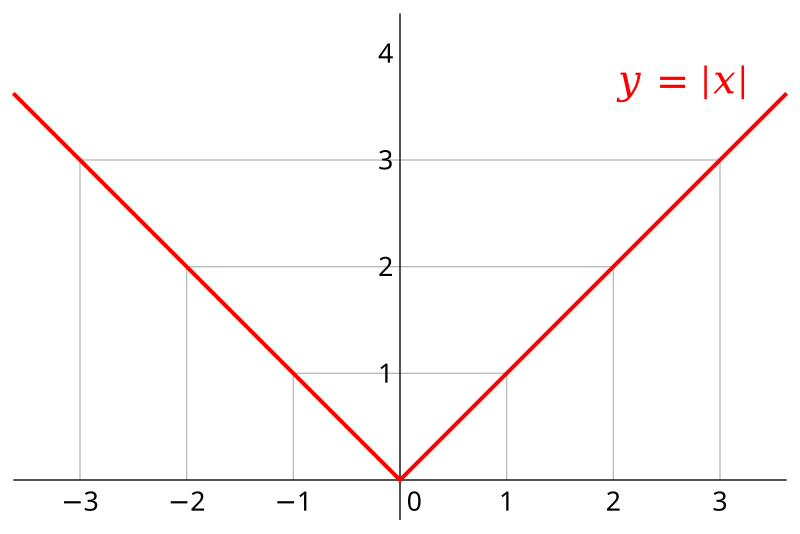
\includegraphics[width=0.5\linewidth, height=5cm, keepaspectratio]{images/basic_math/Absolute_value.svg.png}
            \caption{Absolute Value function/ Modulus Function \cite{wiki/Absolute-value}}
        \end{figure}
    \end{minipage}
\end{table}

\begin{lstlisting}[
    language=Python,
    caption=Absolute value function
]
def get_absolute_value(val):
    if val >= 0:
        return val
    else:
        return -1 * val
\end{lstlisting}

\subsection*{Properties}

\subsubsection*{Fundamental properties} \label{Basic Functions/Absolute Value function or Modulus Function/Fundamental properties}

\begin{customArrayStretch}{1.2}
\begin{tabular}{r l l}
     1. & ${\displaystyle |a|\geq 0}$ & Non-negativity \\

     2. & ${\displaystyle |a|=0\iff a=0}$ & Positive-definiteness \\

     3. & ${\displaystyle |ab|=\left|a\right|\left|b\right|}$ & 	Multiplicativity \\

     4. & ${\displaystyle |a+b|\leq |a|+|b|}$ & 	Subadditivity, specifically the triangle inequality \\
\end{tabular}
\end{customArrayStretch}

\subsubsection*{Additional useful properties \cite{wiki/Absolute-value}} \label{Basic Functions/Absolute Value function or Modulus Function/Additional useful properties}

\begin{customArrayStretch}{1.5}
\begin{tabular}{r l p{13cm}}
     1. & ${\displaystyle {\bigl |}\left|a\right|{\bigr |}=|a|}$ & 	Idempotence (the absolute value of the absolute value is the absolute value) \\

     2. & ${\displaystyle \left|-a\right|=|a|}$ & Evenness (reflection symmetry of the graph) \\

     3. & ${\displaystyle |a-b|=0\iff a=b}$ & 	Identity of indiscernibles (equivalent to positive-definiteness) \\

     4. & ${\displaystyle |a-b|\leq |a-c|+|c-b|}$ & 	Triangle inequality (equivalent to subadditivity) \\

     5. & ${\displaystyle \left|{\dfrac {a}{b}}\right|={\dfrac {|a|}{|b|}}\ }$ (if ${\displaystyle b\neq 0}$) & 	Preservation of division (equivalent to multiplicativity) \\

     6. & ${\displaystyle |a-b|\geq {\bigl |}\left|a\right|-\left|b\right|{\bigr |}}$ & 	Reverse triangle inequality (equivalent to subadditivity) \\
\end{tabular}
\end{customArrayStretch}

\subsection*{Inequalities} \label{Basic Functions/Absolute Value function or Modulus Function/Inequalities}

\begin{enumerate}
    \item ${\displaystyle |a|\leq b\iff -b\leq a\leq b}$
    \hfill \cite{wiki/Absolute-value}

    \item ${\displaystyle |a|\geq b\iff b\leq a\leq -b\ }$
    \hfill \cite{wiki/Absolute-value}
\end{enumerate}

\subsection*{Derivative} \label{Basic Functions/Absolute Value function or Modulus Function/Derivative}

\begin{enumerate}
    \item $
        {\displaystyle {\dfrac {d\left|x\right|}{dx}}={\dfrac {x}{|x|}}={\begin{cases}-1&x<0\\1&x>0\end{cases}}}
    $
    \hfill \cite{wiki/Absolute-value}

    \item $
        {\displaystyle {d \over dx}f(|x|)={x \over |x|}(f'(|x|))}
    $ \hfill (discontinuous at $x=0$)
    \hfill \cite{wiki/Absolute-value}

    \item $
        {\displaystyle {d \over dx}|f(x)|={f(x) \over |f(x)|}f'(x)}
    $ \hfill (discontinuous at $f(x)=0$)
    \hfill \cite{wiki/Absolute-value}
\end{enumerate}


\subsection*{Anti-derivative/ Integral} \label{Basic Functions/Absolute Value function or Modulus Function/Anti-derivative or Integral}

$
    {\displaystyle \dint \left|x\right|dx={\dfrac {x\left|x\right|}{2}}+C}
$
\hfill \cite{wiki/Absolute-value}












\section{Exponential Function ($\exp\dCurlyBrac{x}$, $\exp(x)$)}

$
    \exp\dCurlyBrac{x} = \exp(x) = e^x
$





\section{Sign Function ($\tSgn(x)$)}

$
    \tSgn(x)
    = \begin{cases}
        1 & \text{ if } x>0 \\
        0 & \text{ if } x=0 \\
        -1 & \text{ if } x<0
    \end{cases}
$
\hfill \cite{statistics/book/Statistics-for-Data-Scientists/Maurits-Kaptein}






















\chapter{Advanced Functions}


\section{Gauss error function ($\text{erf}(z)$)}

\[
    {\displaystyle \operatorname {erf} (z)={\dfrac {2}{\sqrt {\pi }}}\int _{0}^{z}e^{-t^{2}}\,\mathrm {d} t.}
    \hfill \text{\cite{wiki/Error_function}}
\]



\section{Gamma Function $\Gamma(x)$}

$
    \Gamma(z) = \begin{cases}
        \dint_{0}^{\infty} x^{z-1} e^{-x} dx & \text{ in general} \\
        (k-1)! & \text{ when $k$ is integer}
    \end{cases}
$
\hfill \cite{statistics/book/Statistics-for-Data-Scientists/Maurits-Kaptein}




















\partition{Data}
\chapter{Data}

\section{Measurement Levels \cite{statistics/book/Statistics-for-Data-Scientists/Maurits-Kaptein}}\label{Data/Measurement-Levels}

\subsection{Nominal, Ordinal, Interval and Ratio \cite{statistics/book/Statistics-for-Data-Scientists/Maurits-Kaptein}}\label{Data/Measurement-Levels/Nominal, Ordinal, Interval and Ratio}

\label{Data/Measurement-Levels/Nominal, Ordinal, Interval and Ratio/Categorical Data}
\label{Data/Measurement-Levels/Nominal, Ordinal, Interval and Ratio/Numerical Data}
\label{Data/Measurement-Levels/Nominal, Ordinal, Interval and Ratio/Nominal}
\label{Data/Measurement-Levels/Nominal, Ordinal, Interval and Ratio/Ordinal}
\label{Data/Measurement-Levels/Nominal, Ordinal, Interval and Ratio/Interval}
\label{Data/Measurement-Levels/Nominal, Ordinal, Interval and Ratio/Ratio}

\begin{table}[H]
    \hfill
    \begin{minipage}[H]{0.25\linewidth}
        \textbf{Levels}: \cite{statistics/book/Statistics-for-Data-Scientists/Maurits-Kaptein}
        \begin{enumerate}
            \item Nominal
            \item Ordinal
            \item Interval
            \item Ratio
        \end{enumerate}
    \end{minipage}
    \hfill
    \begin{minipage}[H]{0.65\linewidth}
        \begin{table}[H]
            \centering
            \begin{tabular}{|p{5cm}|c|c|c|c|}
                \hline
                & \multicolumn{2}{c|}{\textbf{Categorical Data}} & \multicolumn{2}{c|}{\textbf{Numerical Data}} \\ 
                
                \hline
                & \textbf{Nominal} & \textbf{Ordinal} & \textbf{Interval} & \textbf{Ratio} \\ \hline
                
                Distinction between groups / individuals & \checkmark & \checkmark & \checkmark & \checkmark \\ \hline
                
                Imposes logical Order & \xmark & \checkmark & \checkmark & \checkmark \\ \hline
                
                Provides a magnitude of the differences in some unit & \xmark & \xmark & \checkmark & \checkmark \\ \hline
                
                A clear reference point or "0" & \xmark & \xmark & \xmark & \checkmark \\ \hline
            \end{tabular}
            \caption{Data: Measurement Levels: Nominal, Ordinal, Interval and Ratio \cite{statistics/book/Statistics-for-Data-Scientists/Maurits-Kaptein}}
        \end{table}
    \end{minipage}
    \hfill
\end{table}

\vspace{0.3cm}

\textbf{Note}:
\begin{enumerate}
    \item Each consecutive measurement level contains as much "information" - in a fairly loose sense of the word - as the previous one and more. \cite{statistics/book/Statistics-for-Data-Scientists/Maurits-Kaptein}
\end{enumerate}


\subsection{Continuous vs Discrete numerical data \cite{statistics/book/Statistics-for-Data-Scientists/Maurits-Kaptein}}\label{Data/Measurement-Levels/Continuous vs Discrete numerical data}

\label{Data/Measurement-Levels/Continuous vs Discrete numerical data/Continuous numerical data}
\label{Data/Measurement-Levels/Continuous vs Discrete numerical data/Discrete numerical data}

\begin{enumerate}
    \item Continuous variables can assume any value.\\
    This means that the continuous variable can attain any value between two different values, no matter how close the two values are.\\
    \textbf{Example}: temperature, weight, and age

    \item Discrete variables cannot assume any value between 2 values\\
    \textbf{Example}: number of text messages, accidents, microorganisms, students, etc.
\end{enumerate}


\subsection{Outliers \cite{statistics/book/Statistics-for-Data-Scientists/Maurits-Kaptein}}\label{Data/Measurement-Levels/Outliers}

\begin{enumerate}
    \item An outlier is a data point that significantly deviates from other observations in a dataset. \cite{common/online/chatgpt}

    \item Caused by Natural variability in the data or measurement errors. \cite{common/online/chatgpt}

    \item Typically identified using statistical methods like the IQR (Interquartile Range), Z-score, or visualization techniques (e.g., box plots). \cite{common/online/chatgpt}

    \item Outliers are not necessarily incorrect; they may represent rare but valid observations. \cite{common/online/chatgpt}
    
\end{enumerate}


\vspace{0.3cm}

\textbf{Examples}:
\begin{enumerate}
    \item In a dataset of human heights, a person measuring 250 cm might be an outlier but not necessarily unrealistic if it’s a rare case of gigantism. \cite{common/online/chatgpt}
\end{enumerate}


\vspace{0.3cm}
\textbf{Handling/ Dealing with Outliers}:
\begin{enumerate}
    \item Ignore these abnormalities and go ahead with the data. \cite{statistics/book/Statistics-for-Data-Scientists/Maurits-Kaptein}

    \item Delete/ remove the suspected records/ entries. \cite{statistics/book/Statistics-for-Data-Scientists/Maurits-Kaptein}

    \item Substitute them, using statistical methods, with a more plausible alternative. (aka \textbf{imputation}) \cite{statistics/book/Statistics-for-Data-Scientists/Maurits-Kaptein}\label{Data/Outliers/imputation}
\end{enumerate}




\subsection{Unrealistic Values \cite{statistics/book/Statistics-for-Data-Scientists/Maurits-Kaptein}}\label{Data/Measurement-Levels/Unrealistic Values}

\begin{enumerate}
    \item An unrealistic value is a data point that is not plausible within the context of the dataset, often due to data entry errors or faulty sensors. \cite{common/online/chatgpt}

    \item Caused by Human error, sensor malfunction, or corruption during data transmission. \cite{common/online/chatgpt}

    \item Typically identified using domain knowledge or logical constraints. \cite{common/online/chatgpt}

    \item Unlike outliers, unrealistic values are generally not useful and need correction or removal. \cite{common/online/chatgpt}

\end{enumerate}

\vspace{0.3cm}

\textbf{Examples}:
\begin{enumerate}
    \item A recorded body temperature of 200°C for a human is unrealistic, as it’s physically impossible for a person to survive at that temperature. \cite{common/online/chatgpt}

    \item Negative age of a person \cite{common/online/chatgpt}

    \item Missing values \cite{statistics/book/Statistics-for-Data-Scientists/Maurits-Kaptein}

    \item Incorrect datatype of value \cite{statistics/book/Statistics-for-Data-Scientists/Maurits-Kaptein}
\end{enumerate}

\vspace{0.3cm}
\textbf{Handling/ Dealing with Unrealistic values}:
\begin{enumerate}
    \item Delete/ remove the suspected records/ entries. \cite{statistics/book/Statistics-for-Data-Scientists/Maurits-Kaptein}
    
\end{enumerate}





\section{Describing Data \cite{statistics/book/Statistics-for-Data-Scientists/Maurits-Kaptein}} \label{Data/Describing Data}

Some \textbf{descriptive statistics}\label{Data/Describing Data/descriptive statistics} (or just \textbf{descriptives}\label{Data/Describing Data/descriptives}) that we introduce are often used for data of a certain measurement level. \cite{statistics/book/Statistics-for-Data-Scientists/Maurits-Kaptein}

\subsection{Frequency/ Frequency table \cite{statistics/book/Statistics-for-Data-Scientists/Maurits-Kaptein}}\label{Data/Describing Data/Frequency or Frequency table}

\textbf{Measurement levels}: Nominal and ordinal data

\vspace{0.3cm}

\begin{enumerate}
    \item Frequencies are often uninformative for interval or ratio variables. \cite{statistics/book/Statistics-for-Data-Scientists/Maurits-Kaptein}\\
        if there are lots and lots of different possible values, all of them will have a count of just one. \cite{statistics/book/Statistics-for-Data-Scientists/Maurits-Kaptein}\\
        This is often tackled by discretizing (or "\textbf{binning}”\label{Data/Describing Data/Frequency or Frequency table/binning}) the variable (which, note, effectively "throws away” some of the information in the data). \cite{statistics/book/Statistics-for-Data-Scientists/Maurits-Kaptein}

    
\end{enumerate}


\subsubsection{(Absolute) Frequency/ (Absolute) Frequency table \cite{statistics/book/Statistics-for-Data-Scientists/Maurits-Kaptein}}\label{Data/Describing Data/Frequency or Frequency table/Absolute}

\begin{enumerate}
    \item It refers to the count of occurrences of a particular value or category in a dataset. \cite{common/online/chatgpt}

    \item Simple count, no further processing. \cite{common/online/chatgpt}

    \item \textbf{Use Case}: Helpful in creating bar charts or histograms. \cite{common/online/chatgpt}
\end{enumerate}



\subsubsection{Cumulative Frequency/ Cumulative Frequency table \cite{statistics/book/Statistics-for-Data-Scientists/Maurits-Kaptein}}\label{Data/Describing Data/Frequency or Frequency table/Cumulative}

\begin{enumerate}
    \item It is the running total of frequencies up to a certain value or class. \cite{common/online/chatgpt}

    \item Each cumulative frequency includes its own frequency plus all previous frequencies. \cite{common/online/chatgpt}

    \item \textbf{Use Case}: Useful in percentile calculations and ogive graphs. \cite{common/online/chatgpt}

    \item The cumulative frequency makes more sense for ordinal data than for nominal data, since ordinal data can be ordered in size, which is not possible for nominal data. \cite{statistics/book/Statistics-for-Data-Scientists/Maurits-Kaptein}
\end{enumerate}

\begin{table}[H]
    \begin{minipage}[H]{0.3\linewidth}
    $
        \begin{aligned}
            CF_i 
                &= CF_{i-1} + F_{i} \\
                &= \sum_{k=1}^{i} F_{k}
        \end{aligned}
    $
    \end{minipage}
    \begin{minipage}[H]{0.65\linewidth}
        \begin{table}[H]
            \begin{tabular}{l l}
                $CF_i$ & Cumulative Frequency at the current value \\ 
                $CF_{i-1}$ & Cumulative Frequency at the previous value \\ 
                $F_i$ & Frequency at the current value \\ 
            \end{tabular}
            \caption*{Notations}
        \end{table}
    \end{minipage}
\end{table}


\subsubsection{Relative Frequency/ Relative Frequency table \cite{statistics/book/Statistics-for-Data-Scientists/Maurits-Kaptein}}\label{Data/Describing Data/Frequency or Frequency table/Relative}

\begin{enumerate}
    \item It shows the proportion of each category relative to the total number of observations. \cite{common/online/chatgpt}

    \item Expressed as a fraction, decimal, or percentage. \cite{common/online/chatgpt}

    \item \textbf{Use Case}: Ideal for creating pie charts and understanding distribution proportions. \cite{common/online/chatgpt}
\end{enumerate}


\begin{table}[H]
    \begin{minipage}{0.3\linewidth}
        \[
            \begin{aligned}
                RF_i 
                    &= \dfrac{F_{i}}{\dsum_{k=1}^{N} F_{k}}
            \end{aligned}
        \]
    \end{minipage}
    \begin{minipage}{0.65\linewidth}
        \begin{table}[H]
            \begin{tabular}{l l}
                $RF_i$ & Relative Frequency \\
                $F_i$ & Frequency of the value \\ 
                $N$ & Total number of observations \\ 
            \end{tabular}
            \caption*{Notations}
        \end{table}
    \end{minipage}
\end{table}




\subsubsection{Cumulative Relative Frequency/ Cumulative Relative Frequency table \cite{statistics/book/Statistics-for-Data-Scientists/Maurits-Kaptein}}\label{Data/Describing Data/Frequency or Frequency table/Cumulative Relative}

\begin{enumerate}
    \item Cumulative relative frequency is the accumulation of the relative frequencies of data points up to a certain value. \cite{common/online/chatgpt}

    \item It indicates the proportion of data points that are less than or equal to a particular value. \cite{common/online/chatgpt}

    \item \textbf{Use Cases}:
    \begin{enumerate}
        \item Identifying percentiles and median.

        \item Visualizing with a cumulative relative frequency graph (Ogive).

        \item Understanding data distribution by determining the proportion of values below a specific threshold.
    \end{enumerate}
\end{enumerate}



\begin{table}[H]
    \begin{minipage}{0.3\linewidth}
        \[
            \begin{aligned}
                CRF_i 
                    &= \dfrac{\dsum_{k=1}^{i} F_{k}}{\dsum_{k=1}^{N} F_{k}}
            \end{aligned}
        \]
    \end{minipage}
    \begin{minipage}{0.65\linewidth}
        \begin{table}[H]
            \begin{tabular}{l l}
                $CRF_i$ & Cumulative Relative Frequency \\
                $F_i$ & Frequency of the value \\ 
                $N$ & Total number of observations \\ 
            \end{tabular}
            \caption*{Notations}
        \end{table}
    \end{minipage}
\end{table}





\subsection{Central Tendency \cite{statistics/book/Statistics-for-Data-Scientists/Maurits-Kaptein}}\label{Data/Describing Data/Central Tendency}

\begin{enumerate}
     \item When we work with numerical data, we often want to know something about the "central value" or "middle value" of the variable, also referred to as the \textbf{location}\label{Data/Describing Data/Central Tendency/location} of the data. \cite{statistics/book/Statistics-for-Data-Scientists/Maurits-Kaptein}
\end{enumerate}


\subsubsection{(Arithmetic) mean/ average \cite{statistics/book/Statistics-for-Data-Scientists/Maurits-Kaptein}} \label{Data/Describing Data/Central Tendency/(Arithmetic) mean or average}

\begin{table}[H]
    \begin{minipage}{0.3\linewidth}
        $
            \bar{x} = \dfrac{1}{n} \dsum_{i=1}^{n} x_i
        $
    \end{minipage}
    \begin{minipage}{0.65\linewidth}
        \begin{table}[H]
            \begin{tabular}{l l}
                $\bar{x}$ & mean \\
                $x_i$ & item \\
                $n$ & number of items \\
            \end{tabular}
            \caption*{Notations}
        \end{table}
    \end{minipage}
\end{table}



\subsubsection{Mode \cite{statistics/book/Statistics-for-Data-Scientists/Maurits-Kaptein}} \label{Data/Describing Data/Central Tendency/Mode}

\begin{enumerate}
    \item The mode is merely the most frequently occurring value. \cite{statistics/book/Statistics-for-Data-Scientists/Maurits-Kaptein}

    \item There might be multiple modes. \cite{statistics/book/Statistics-for-Data-Scientists/Maurits-Kaptein}
    
\end{enumerate}



\subsubsection{Median \cite{statistics/book/Statistics-for-Data-Scientists/Maurits-Kaptein}} \label{Data/Describing Data/Central Tendency/Median}

\begin{enumerate}
    \item The median is a value that divides the ordered data from small to large (or large to small) into two equal parts: 50\% of the data is below the median and 50\% is above. \cite{statistics/book/Statistics-for-Data-Scientists/Maurits-Kaptein}

    \item The median is not necessarily a value that is present in the data. \cite{statistics/book/Statistics-for-Data-Scientists/Maurits-Kaptein}
\end{enumerate}


\vspace{0.3cm}
\textbf{Steps}:
\begin{enumerate}
    \item sort the data

    \item choose the middle-most value when $n$ is \textbf{odd}\\
        average of the two middle values when $n$ is \textbf{even}
\end{enumerate}



\subsubsection{Quantiles \cite{statistics/book/Statistics-for-Data-Scientists/Maurits-Kaptein}} \label{Data/Describing Data/Central Tendency/Quantiles}

\begin{enumerate}
    \item A quantile $x_q$ is a value that splits the ordered data of a variable $x$ into two parts: \cite{statistics/book/Statistics-for-Data-Scientists/Maurits-Kaptein}
    \begin{enumerate}
        \item $q \cdot 100\%$ of the data is below the value $x_q$

        \item $(1 - q) \cdot 100\%$ of the data is above the value $x_q$
    \end{enumerate}
    
    \item The parameter $q$ can take any value in the interval $[0, 1]$. \cite{statistics/book/Statistics-for-Data-Scientists/Maurits-Kaptein}

    \item Quantiles can be calculated in different ways, depending on the way we "interpolate" between two values. \cite{statistics/book/Statistics-for-Data-Scientists/Maurits-Kaptein} \\
    We could map the ordered values \textit{equally spaced} on the interval $(0, 1)$, where the \textit{i}th ordered value of the data is positioned at the level $q_i = {i}/{(n + 1)}$ in the interval $(0, 1)$, with $n$ being the number of data points. \cite{statistics/book/Statistics-for-Data-Scientists/Maurits-Kaptein} \\
    R uses $q_i = (i - 1)/(n - 1)$ for quantiles. \cite{statistics/book/Statistics-for-Data-Scientists/Maurits-Kaptein} \\
    \textbf{Example}: \cite{statistics/book/Statistics-for-Data-Scientists/Maurits-Kaptein}
    \begin{enumerate}
        \item Data points: $\dCurlyBrac{2, 5, 6, 4}$ ($n=4$)
        \item Sorted Data points: $\dCurlyBrac{2, 4, 5, 6}$ ($n=4$)
        \item Quantiles:\\[0.2cm]
        \begin{tabular}{|l|c|c|c|}
            \hline
            $i$ & $x_i$ & $q_i = i/(n+1) = i/5$ & $q_i = (i-1)/(n-1) = (i-1)/3$ \\ [0.1cm]
            \hline
            $1$ & $2$ & $1/5 = 0.2$ & $0$ \\
            $2$ & $4$ & $2/5 = 0.4$ & $1/3$ \\
            $3$ & $5$ & $3/5 = 0.6$ & $2/3$ \\
            $4$ & $6$ & $4/5 = 0.8$ & $1$ \\
            \hline
        \end{tabular}\\

        \item If $x_i = 3 \Rightarrow q_i = 0.3$
    \end{enumerate}
\end{enumerate}




\subsubsection{Quartiles \cite{statistics/book/Statistics-for-Data-Scientists/Maurits-Kaptein}} \label{Data/Describing Data/Central Tendency/Quartiles}

\begin{enumerate}
    \item When $q = 0.25$, $q = 0.50$, and $q = 0.75$ the quantiles are referred to as the first, second, and third quartiles, respectively. \cite{statistics/book/Statistics-for-Data-Scientists/Maurits-Kaptein}
    \label{Data/Describing Data/Central Tendency/Quartiles/first quartile}
    \label{Data/Describing Data/Central Tendency/Quartiles/second quartile}
    \label{Data/Describing Data/Central Tendency/Quartiles/third quartile}

    \item Splits: \\
    \begin{tabular}{r l l l} % Right-align first column, left-align second column
        1. & $q = 0$ & to & $q = 0.25$ \\
        2. & $q = 0.25$ & to & $q = 0.5$ \\
        3. & $q = 0.5$ & to & $q = 0.75$ \\
        4. & $q = 0.75$ & to & $q = 1$ \\
    \end{tabular}
\end{enumerate}



\subsubsection{Deciles \cite{statistics/book/Statistics-for-Data-Scientists/Maurits-Kaptein}} \label{Data/Describing Data/Central Tendency/Deciles}

\begin{enumerate}
    \item We call quantiles deciles when $q$ is restricted to the set $\dCurlyBrac{0.1, 0.2,\cdots, 0.9}$

    \item Splits: \\
    \begin{tabular}{r l l l} % Right-align first column, left-align second column
        1. & $q = 0$ & to & $q = 0.1$ \\
        2. & $q = 0.1$ & to & $q = 0.2$ \\
        && \vdots & \\
        9. & $q = 0.8$ & to & $q = 0.9$ \\
        10. & $q = 0.9$ & to & $q = 1$ \\
    \end{tabular}
\end{enumerate}



\subsubsection{Percentiles \cite{statistics/book/Statistics-for-Data-Scientists/Maurits-Kaptein}} \label{Data/Describing Data/Central Tendency/Percentiles}

\begin{enumerate}
    \item We call quantiles percentiles when $q$ is restricted to the set $\dCurlyBrac{0.01, 0.02,\cdots, 0.99}$

    \item Splits: \\
    \begin{tabular}{r l l l} % Right-align first column, left-align second column
        1. & $q = 0$ & to & $q = 0.01$ \\
        2. & $q = 0.01$ & to & $q = 0.02$ \\
        & & \vdots & \\
        99. & $q = 0.98$ & to & $q = 0.99$ \\
        100. & $q = 0.99$ & to & $q = 1$ \\
    \end{tabular}
\end{enumerate}









\chapter{Visualizing Data} \label{Visualizing Data}

\begin{enumerate}
    \item Visualization, when done well, can make large and even high-dimensional datasets (relatively) easy to interpret. \hfill \cite{statistics/book/Statistics-for-Data-Scientists/Maurits-Kaptein}

    
\end{enumerate}


\begin{lstlisting}[
    language=Python
]
import random
import faker                    # to generate fake data
import numpy as np
import pandas as pd
from tqdm import tqdm           # progress bar

# plotting libraries
import seaborn as sns           
import matplotlib.pyplot as plt

random.seed(0)
np.random.seed(0)
faker.Faker.seed(0)

fake = faker.Faker()
\end{lstlisting}


\clearpage
\section{Box and Whiskers Plot/ Box Plot \cite{data/online/seaborn.boxplot, data/online/matplotlib.pyplot.boxplot}} \label{Visualizing Data/Box and Whiskers Plot or Box Plot}

\begin{lstlisting}[numbers=none]

                     Q1-1.5IQR   Q1   median  Q3   Q3+1.5IQR
                                  |-----:-----|
                  o      |--------|     :     |--------|    o  o
                                  |-----:-----|
                flier             <----------->            fliers
                                       IQR

\end{lstlisting}

\vspace{0.5cm}

\begin{table}[H]
\begin{minipage}[t]{0.35\linewidth}
\begin{figure}[H]
    \centering
    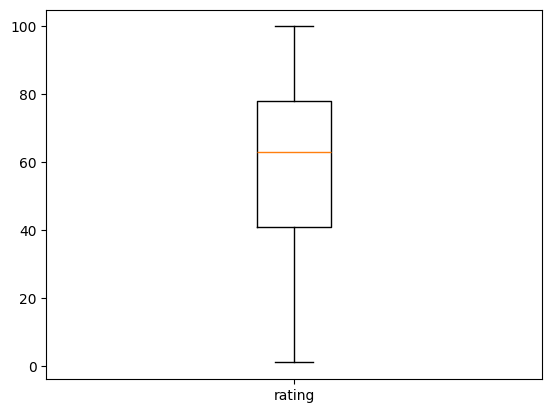
\includegraphics[width=0.9\linewidth, height=10cm, keepaspectratio]{images/data/__visualizations__/plt-box-rating-face-data.png}
    \caption{Box and Whiskers plot (py-plt) output (face\_data.csv)}
\end{figure}
\end{minipage}
\hspace{0.2cm}
\vrule width 1pt
\hspace{0.5cm}
\begin{minipage}[t]{0.57\linewidth}
\begin{lstlisting}[
    language=Python,
    caption=Box and Whiskers Plot: py-plt: face\_data.csv
]
_col = "rating"

plt.boxplot(df[_col])
plt.xticks([1], [_col])
plt.show()
\end{lstlisting}
\end{minipage}
\end{table}



\begin{table}[H]
\begin{minipage}[t]{0.35\linewidth}
\begin{figure}[H]
    \centering
    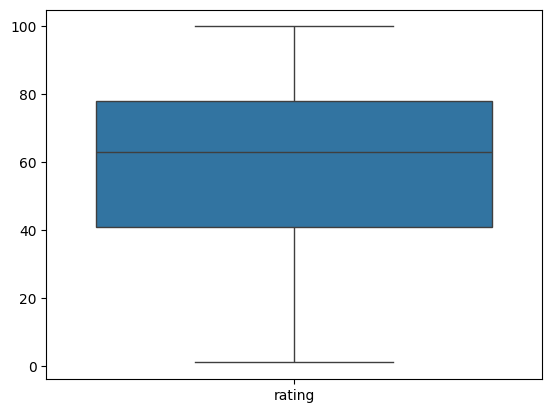
\includegraphics[width=0.9\linewidth, height=10cm, keepaspectratio]{images/data/__visualizations__/sns-box-rating-face-data.png}
    \caption{Box and Whiskers plot (py-sns) output (face\_data.csv)}
\end{figure}
\end{minipage}
\hspace{0.2cm}
\vrule width 1pt
\hspace{0.5cm}
\begin{minipage}[t]{0.57\linewidth}
\begin{lstlisting}[
    language=Python,
    caption=Box and Whiskers Plot: py-sns: face\_data.csv
]
_col = "rating"

sns.boxplot(df[_col])
plt.ylabel("")
plt.xticks([0], [_col])
plt.show()
\end{lstlisting}
\end{minipage}
\end{table}




\begin{enumerate}
    \item A box plot (or box-and-whisker plot) shows the distribution of quantitative data in a way that facilitates comparisons between variables or across levels of a categorical variable.  \hfill \cite{data/online/seaborn.boxplot}
    
    \item The box shows the quartiles of the dataset while the whiskers extend to show the rest of the distribution, except for points that are determined to be “outliers” using a method that is a function of the inter-quartile range. \hfill \cite{data/online/seaborn.boxplot}
\end{enumerate}





\clearpage
\section{Count Plot \cite{data/online/seaborn.countplot}} \label{Visualizing Data/Count Plot}


\begin{table}[H]
\begin{minipage}[t]{0.35\linewidth}
\begin{figure}[H]
    \centering
    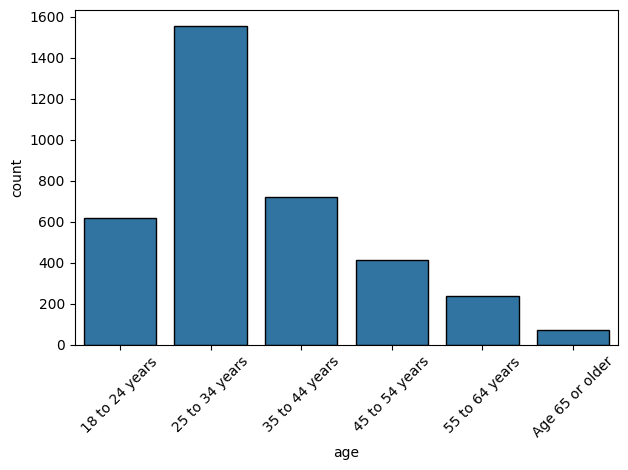
\includegraphics[width=0.9\linewidth, height=10cm, keepaspectratio]{images/data/__visualizations__/sns-countplot-face-data.png}
    \caption{Count plot (py-sns) output (face\_data.csv)}
\end{figure}
\end{minipage}
\hspace{0.2cm}
\vrule width 1pt
\hspace{0.5cm}
\begin{minipage}[t]{0.57\linewidth}
\begin{lstlisting}[
    language=Python,
    caption=Count Plot: py-sns: face\_data.csv
]
vals = df[df["age"] != " "].copy()

sns.countplot(
    x='age', 
    data=vals, 
    order=sorted(vals['age'].unique()), 
    edgecolor='black',
)

plt.xticks(rotation=45)
plt.tight_layout()
plt.show()
\end{lstlisting}
\end{minipage}
\end{table}

\vspace{0.3cm}

\begin{enumerate}
    \item Show the counts of observations in each categorical bin using bars.

    
\end{enumerate}



% \clearpage
\section{Density Plot \cite{data/online/seaborn.displot}} \label{Visualizing Data/Density Plot}

\begin{table}[H]
\begin{minipage}[t]{0.35\linewidth}
\begin{figure}[H]
    \centering
    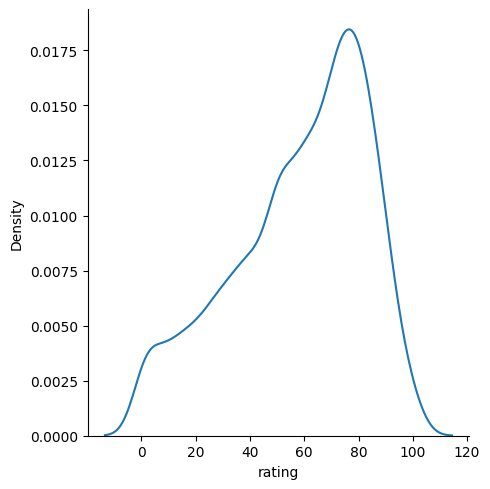
\includegraphics[width=0.9\linewidth, height=10cm, keepaspectratio]{images/data/__visualizations__/sns-density-kde-rating-face-data.png}
    \caption{Density plot (py-sns) output (face\_data.csv)}
\end{figure}
\end{minipage}
\hspace{0.2cm}
\vrule width 1pt
\hspace{0.5cm}
\begin{minipage}[t]{0.57\linewidth}
\begin{lstlisting}[
    language=Python,
    caption=Density Plot: py-sns: face\_data.csv
]
sns.displot(df["rating"], kind="kde")

plt.show()
\end{lstlisting}

\vspace{0.2cm}

\begin{enumerate}
    \item A density plot - at least in this setting - can be considered a “continuous approximation” of a histogram. \hfill \cite{statistics/book/Statistics-for-Data-Scientists/Maurits-Kaptein} \\
    SEE: \fullref{Visualizing Data/Histogram}

    \item It gives per range of values of the continuous variable the probability of observing a value within that range. \hfill \cite{statistics/book/Statistics-for-Data-Scientists/Maurits-Kaptein}


\end{enumerate}

\end{minipage}
\end{table}







\clearpage
\section{Histogram \cite{data/online/seaborn.histplot}} \label{Visualizing Data/Histogram}


\begin{table}[H]
\begin{minipage}[t]{0.35\linewidth}
\begin{figure}[H]
    \centering
    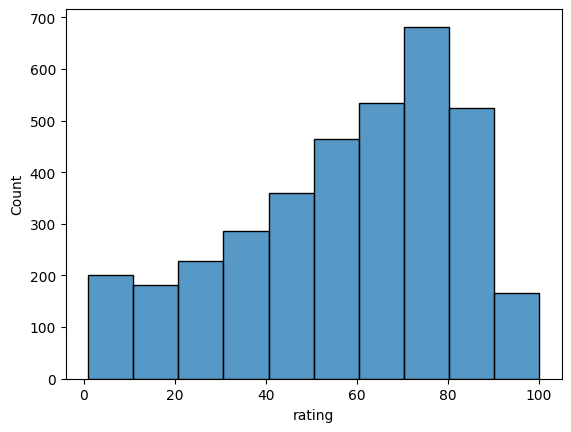
\includegraphics[width=0.9\linewidth, height=10cm, keepaspectratio]{images/data/__visualizations__/sns-hist-rating-face-data.png}
    \caption{Histogram (py-sns) output (face\_data.csv)}
\end{figure}
\end{minipage}
\hspace{0.2cm}
\vrule width 1pt
\hspace{0.5cm}
\begin{minipage}[t]{0.57\linewidth}
\begin{lstlisting}[
    language=Python,
    caption=Histogram: py-sns: face\_data.csv
]
sns.histplot(df["rating"], binwidth=10)
plt.show()
\end{lstlisting}

\vspace{0.2cm}

\begin{enumerate}
    \item A histogram is a classic visualization tool that represents the distribution of one or more variables by counting the number of observations that fall within discrete bins. \hfill \cite{data/online/seaborn.histplot}

    \item A histogram “bins” the data (discretizes it), and subsequently shows the frequency of occurrence in each bin. \hfill \cite{statistics/book/Statistics-for-Data-Scientists/Maurits-Kaptein}
    
    \item It is the continuous variant of the bar chart. \hfill \cite{statistics/book/Statistics-for-Data-Scientists/Maurits-Kaptein}\\
    SEE: \fullref{Visualizing Data/Box and Whiskers Plot or Box Plot}
    
    \item The number of bins selected makes a big difference in the visualization: too few bins obscure the patterns in the data, but too many bins lead to counts of exactly one for each value. \hfill \cite{statistics/book/Statistics-for-Data-Scientists/Maurits-Kaptein}
\end{enumerate}

\end{minipage}
\end{table}


% \clearpage
\section{Pairwise Plot \cite{statistics/book/Statistics-for-Data-Scientists/Maurits-Kaptein, data/online/seaborn.pairplot}} \label{Visualizing Data/Pairwise Plot}


\begin{table}[H]
\begin{minipage}[t]{0.35\linewidth}
\begin{figure}[H]
    \centering
    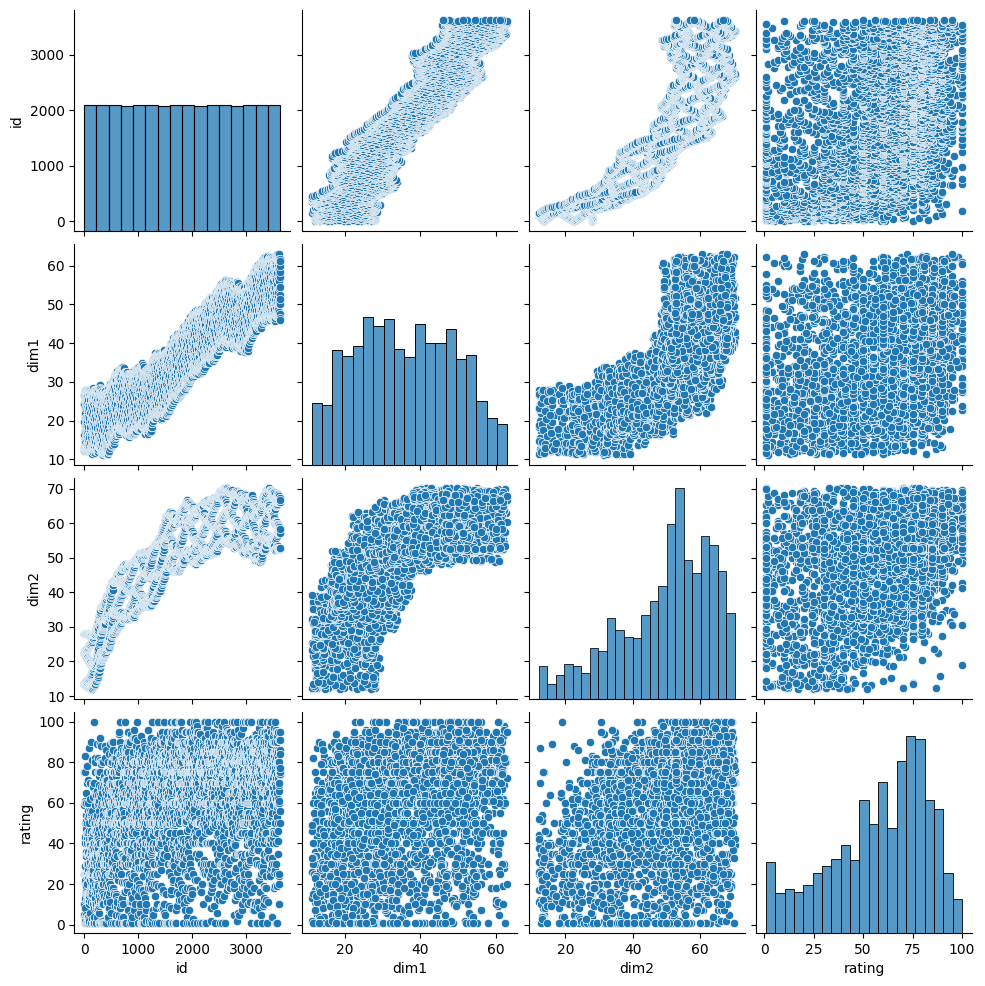
\includegraphics[width=0.9\linewidth, height=10cm, keepaspectratio]{images/data/__visualizations__/sns-pairplot-face-data.png}
    \caption{Pairwise plot (py-sns) output (face\_data.csv)}
\end{figure}
\end{minipage}
\hspace{0.2cm}
\vrule width 1pt
\hspace{0.5cm}
\begin{minipage}[t]{0.57\linewidth}
\begin{lstlisting}[
    language=Python,
    caption=Pairwise Plot: py-sns: face\_data.csv
]
df = pd.read_csv("face_data.csv")
sns.pairplot(df)
\end{lstlisting}

\vspace{0.3cm}

\begin{enumerate}
    \item Plot pairwise relationships in a dataset. \hfill \cite{data/online/seaborn.pairplot}

    \item By default, this is a grid of Axes such that each numeric variable in data will by shared across the y-axes across a single row and the x-axes across a single column. \hfill \cite{data/online/seaborn.pairplot}
    
    \item The diagonal plots are treated differently: a univariate distribution plot is drawn to show the marginal distribution of the data in each column. \hfill \cite{data/online/seaborn.pairplot}
\end{enumerate}
\end{minipage}
\end{table}











\clearpage
\section{Pie Chart \cite{data/online/matplotlib.pyplot.pie}} \label{Visualizing Data/Pie Chart}


\begin{table}[H]
\begin{minipage}[t]{0.35\linewidth}
\begin{figure}[H]
    \centering
    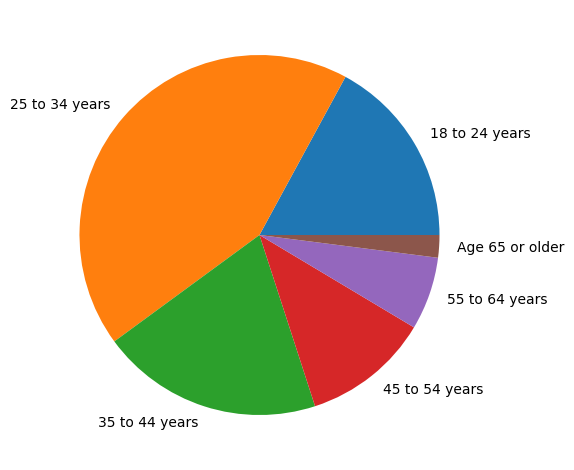
\includegraphics[width=0.9\linewidth, height=10cm, keepaspectratio]{images/data/__visualizations__/plt-pie-age-face-data.png}
    \caption{Pie chart (py-plt) output (face\_data.csv)}
\end{figure}
\end{minipage}
\hspace{0.2cm}
\vrule width 1pt
\hspace{0.5cm}
\begin{minipage}[t]{0.57\linewidth}
\begin{lstlisting}[
    language=Python,
    caption=Pie Chart: py-plt: face\_data.csv
]
vals = df[df["age"] != " "].copy()

labels, counts = np.unique(
    vals['age'],
    return_counts=True
)

plt.pie(counts, labels=labels)

plt.tight_layout()
plt.show()
\end{lstlisting}
\end{minipage}
\end{table}



\clearpage
\section{Scatter Plot \cite{data/online/seaborn.scatterplot, data/online/seaborn.scatterplot, data/online/wiki/Scatter_plot}} \label{Visualizing Data/Scatter Plot}


\begin{table}[H]
\begin{minipage}[t]{0.35\linewidth}
\begin{figure}[H]
    \centering
    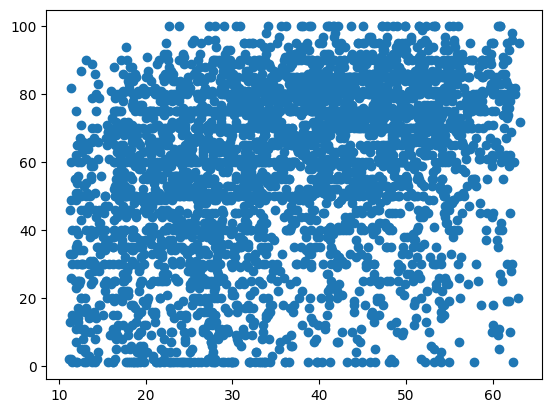
\includegraphics[width=0.9\linewidth, height=10cm, keepaspectratio]{images/data/__visualizations__/plt-scatter-dim1-rating-face-data.png}
    \caption{Scatter Plot (py-plt) output (face\_data.csv)}
\end{figure}
\end{minipage}
\hspace{0.2cm}
\vrule width 1pt
\hspace{0.5cm}
\begin{minipage}[t]{0.57\linewidth}
\begin{lstlisting}[
    language=Python,
    caption=Scatter Plot: py-plt: face\_data.csv
]
plt.scatter(df["dim1"], df["rating"])

plt.show()
\end{lstlisting}
\end{minipage}
\end{table}

\begin{table}[H]
\begin{minipage}[t]{0.35\linewidth}
\begin{figure}[H]
    \centering
    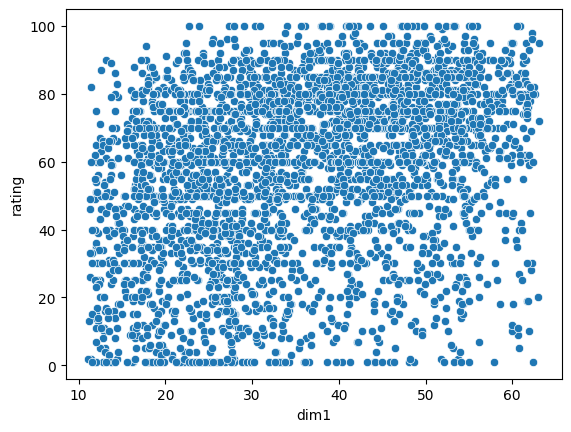
\includegraphics[width=0.9\linewidth, height=10cm, keepaspectratio]{images/data/__visualizations__/sns-scatter-dim1-rating-face-data.png}
    \caption{Scatter Plot (py-sns) output (face\_data.csv)}
\end{figure}
\end{minipage}
\hspace{0.2cm}
\vrule width 1pt
\hspace{0.5cm}
\begin{minipage}[t]{0.57\linewidth}
\begin{lstlisting}[
    language=Python,
    caption=Scatter Plot: py-sns: face\_data.csv
]
sns.scatterplot(df, x="dim1", y="rating")

plt.show()
\end{lstlisting}
\end{minipage}
\end{table}





\begin{enumerate}
    \item A scatter plot, also called a \textbf{scatterplot}, \textbf{scatter graph}\label{Visualizing Data/scatter graph}, \textbf{scatter chart}\label{Visualizing Data/scatter chart}, \textbf{scattergram}\label{Visualizing Data/scattergram}, or \textbf{scatter diagram}\label{Visualizing Data/scatter diagram}, is a type of plot or mathematical diagram using Cartesian coordinates to display values for typically two variables for a set of data. \hfill \cite{data/online/wiki/Scatter_plot}
    
    \item If the points are coded (color/shape/size), one additional variable can be displayed. \hfill \cite{data/online/wiki/Scatter_plot}
    
    \item The data are displayed as a collection of points, each having the value of one variable determining the position on the horizontal axis and the value of the other variable determining the position on the vertical axis. \hfill \cite{data/online/wiki/Scatter_plot}
\end{enumerate}











\partition{Mathematics: Statistics}
\chapter{Sampling Plans}\label{Sampling Plans}


\begin{figure}[H]
    \centering
    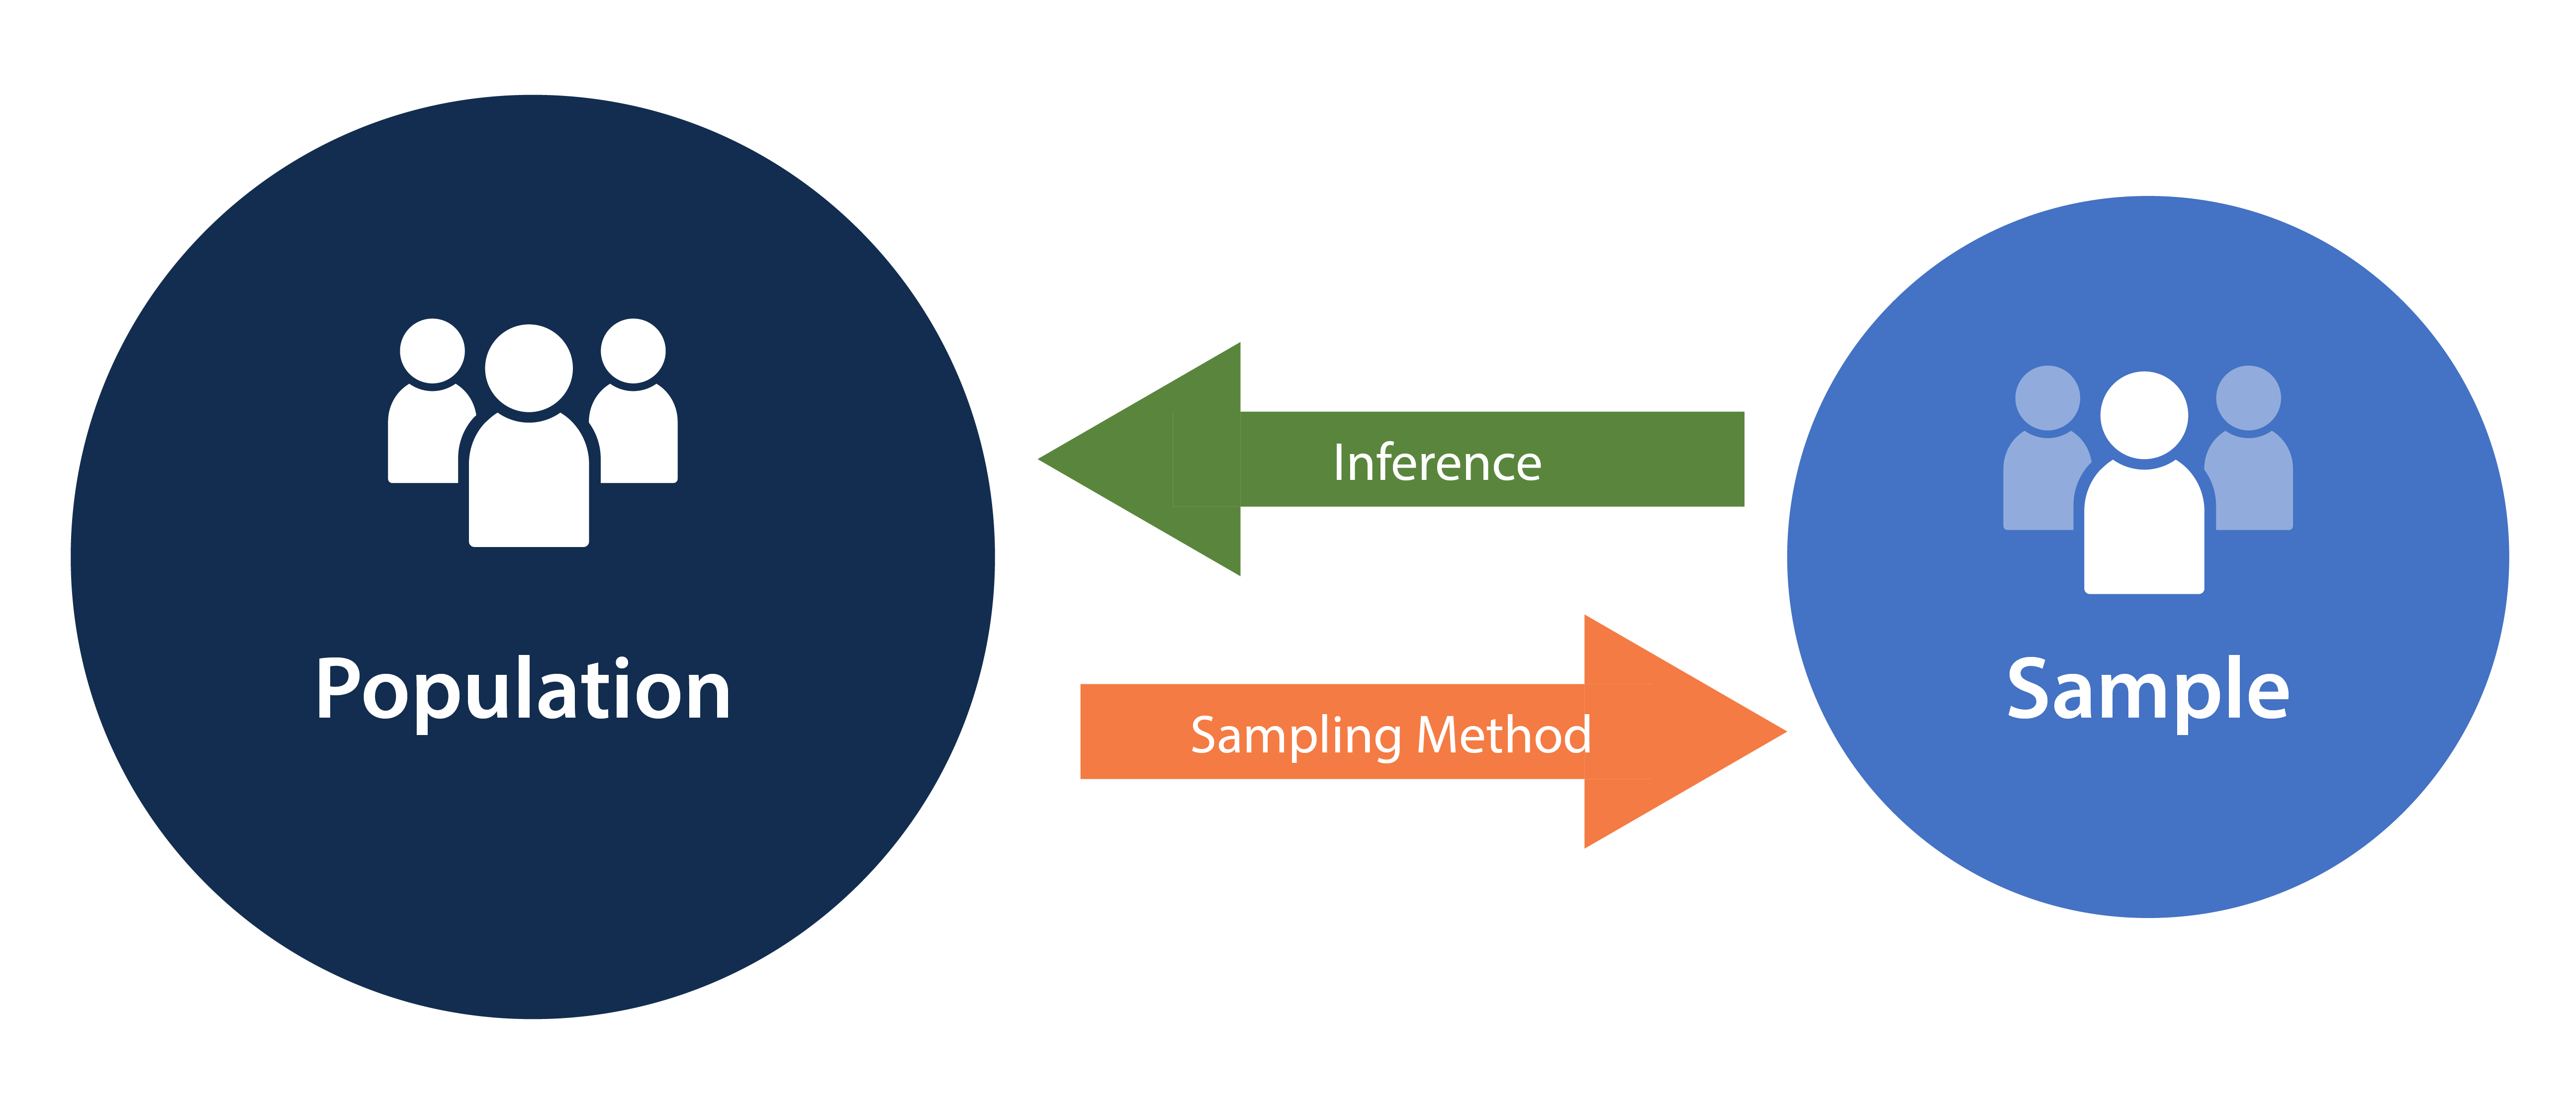
\includegraphics[
        width=0.5\linewidth,
        height=5cm,
        keepaspectratio
    ]{images/statistics/sampling-plan.png}

    \caption{Sampling Plan: Relation between Population and Sample}
\end{figure}


\begin{enumerate}
    \item \textbf{Statistical Inference}\label{Sampling Plans/Statistical Inference}: To extend your conclusions beyond the observed data.
    The field of \textbf{inferential statistics} tries to use the information from a sample to make statements or decisions about the population of interest.
    It takes into account the uncertainty that the information is coming from sampling and does not perfectly represent the population, since another sample would give different outcomes.
    An important aspect of inferential statistics is estimation of the population parameters of interest.
    \hfill \cite{statistics/book/Statistics-for-Data-Scientists/Maurits-Kaptein}

    \item Sampling procedures are formal \textit{probabilistic approaches} to help collect units from the population for the sample.
    \hfill \cite{statistics/book/Statistics-for-Data-Scientists/Maurits-Kaptein}

    \item \textbf{Population}\label{Sampling Plans/Population}: The complete set of units that we would like to say something about is called the (target) population.
    \hfill \cite{statistics/book/Statistics-for-Data-Scientists/Maurits-Kaptein}
    \\
    In principle we would expect that a population is \textbf{always finite}, since an infinite number of units does not exist in real life. However, populations are often treated as infinite. One reason is that populations can be really really large.
    \hfill \cite{statistics/book/Statistics-for-Data-Scientists/Maurits-Kaptein}
    \\
    It is mathematically often more convenient (as we will see later) to assume that such a population is infinite.
    \hfill \cite{statistics/book/Statistics-for-Data-Scientists/Maurits-Kaptein}
    \\
    Properly defining or describing a population can be difficult. Furthermore, even if the population is established, measuring all units is often impossible or too elaborate. This means that information about the population can only be obtained by considering a subset of the population.
    \hfill \cite{statistics/book/Statistics-for-Data-Scientists/Maurits-Kaptein}

    \item \textbf{Sample}\label{Sampling Plans/Sample}: The set of units for which we have obtained data is referred to as the sample.
    \hfill \cite{statistics/book/Statistics-for-Data-Scientists/Maurits-Kaptein}
    \\
    The sample is typically a subset of the population, although in theory the sample can form the whole population or the sample can contain units that are not from the target population.
    \hfill \cite{statistics/book/Statistics-for-Data-Scientists/Maurits-Kaptein}

    \item \textbf{Representative Sample}\label{Sampling Plans/Representative Sample}:  A representative sample can be intuitively defined as a sample of units that has approximately the same distribution of characteristics as the population from which it was drawn.
    \hfill \cite{statistics/book/Statistics-for-Data-Scientists/Maurits-Kaptein}
    \\
    Representative sampling is also referred to as random or probability sampling.
    \hfill \cite{statistics/book/Statistics-for-Data-Scientists/Maurits-Kaptein}

    \item \textbf{Unit}\label{Sampling Plans/Unit}: A unit is usually a concrete or physical thing for which we would like to measure its characteristics.
    \hfill \cite{statistics/book/Statistics-for-Data-Scientists/Maurits-Kaptein}

    \item \textbf{Estimates}\label{Sampling Plans/Estimates}: In terms of statistical inference, the calculations on the sample data are referred to as estimates for the theoretical value in the whole population.
    \hfill \cite{statistics/book/Statistics-for-Data-Scientists/Maurits-Kaptein}

    \item \textbf{Estimators}\label{Sampling Plans/Estimators}: quantities that we compute using the data in our sample to say something about the population.
    \hfill \cite{statistics/book/Statistics-for-Data-Scientists/Maurits-Kaptein}

    \item \textbf{Realization}\label{Sampling Plans/realization}: The values in the sample are referred to as a realization from the population.
    \hfill \cite{statistics/book/Statistics-for-Data-Scientists/Maurits-Kaptein}

    %%%%%%%%%%%%%%%%%%%%%%%%%%%%%%%%%%%%%%%%%%%%%%%%%%%%%%%%%%%%%%%%%%%%%%%%%%%%%%
    \vspace{0.5cm}

    \item Reasons for sample instead of population:
    \begin{enumerate}
        \item In many applications we really can’t measure the complete population. For instance, one of the tests applied to aircraft engines is the “frozen bird test”.
        \hfill \cite{statistics/book/Statistics-for-Data-Scientists/Maurits-Kaptein}

        \item Time, space, or budget restrictions often do not allow us to measure all units from a population.
        \hfill \cite{statistics/book/Statistics-for-Data-Scientists/Maurits-Kaptein}

        \item  Big data itself may be an argument for sampling. If we have a very large sample or we have been able to measure all units from the population, the resulting dataset can be so large that it becomes impossible to analyze the full data at one computer.
        \hfill \cite{statistics/book/Statistics-for-Data-Scientists/Maurits-Kaptein}
    \end{enumerate}

    \item A non-representative sample implies that we do not know the exact process by which units in the population became part of the sample.
    \hfill \cite{statistics/book/Statistics-for-Data-Scientists/Maurits-Kaptein}

    \item If we know which sampling procedure was applied to collect the units for the sample, we would also know how close the calculations or statistics would be to the theoretical value in the whole population.
    \hfill \cite{statistics/book/Statistics-for-Data-Scientists/Maurits-Kaptein}
    \\
    Thus the sampling procedure and the choice of calculation on the sample data (\\
    \nameref{Data/Describing Data/Central Tendency/(Arithmetic) mean or average}, \\
    \nameref{Data/Describing Data/Central Tendency/Median},\\
    \nameref{Data/Describing Data/Central Tendency/Quartiles/first quartile}, \\
    \nameref{Data/Describing Data/Central Tendency/Standard Deviation}\\
    etc.) would make statistical inference mathematically precise and it would therefore help us when making statements beyond the sample data.
    \hfill \cite{statistics/book/Statistics-for-Data-Scientists/Maurits-Kaptein}


\end{enumerate}

\section{Generic Formulation \cite{statistics/book/Statistics-for-Data-Scientists/Maurits-Kaptein}}

\begin{customArrayStretch}{1.3}
\begin{longtable}{>{\RaggedRight\arraybackslash}p{4cm} >{\centering\arraybackslash}p{0.5cm} p{10.5cm}}

\hhline{=:=:=} \endfirsthead
\hhline{=:=:=} \endhead
\hhline{=:=:=} \endfoot
\hhline{=:=:=} \endlastfoot


\textbf{Population Size} &
    $N$ &
    \hfill \cite{statistics/book/Statistics-for-Data-Scientists/Maurits-Kaptein}
    \\ \hline

\textbf{Sample Size} &
    $n$ &
    \begin{minipage}{10.3cm}
        \vspace{0.15cm}
        \begin{enumerate}
            \item $n \leq N$
            \hfill \cite{statistics/book/Statistics-for-Data-Scientists/Maurits-Kaptein}

        \end{enumerate}
        \vspace{0.15cm}
    \end{minipage}
    \\ \hline

\textbf{Number of Possible Samples} &
    $K$ &
    \begin{minipage}{10.3cm}
        \vspace{0.15cm}
        \begin{enumerate}
            \item exact value of $K$ depends on the sampling plan
            \hfill \cite{statistics/book/Statistics-for-Data-Scientists/Maurits-Kaptein}

        \end{enumerate}
        \vspace{0.15cm}
    \end{minipage}
    \\ \hline

\textbf{Population} &
    $\Omega$ &
    \begin{minipage}{10.3cm}
        \vspace{0.15cm}
        \begin{enumerate}
            \item $\Omega = \dCurlyBrac{1,2,\cdots,N}$
            \hfill \cite{statistics/book/Statistics-for-Data-Scientists/Maurits-Kaptein}

            \item $\Omega = \dbigcup_{k=1}^K S_k$
            \hfill \cite{statistics/book/Statistics-for-Data-Scientists/Maurits-Kaptein}
        \end{enumerate}
        \vspace{0.15cm}
    \end{minipage}
    \\ \hline


\textbf{Sample} &
    $S_k$ &
    \begin{minipage}{10.3cm}
        \vspace{0.15cm}
        \begin{enumerate}
            \item Subset of Population
            \hfill \cite{statistics/book/Statistics-for-Data-Scientists/Maurits-Kaptein}

            \item $k \in \dCurlyBrac{1,2,\cdots, K}$
            \hfill \cite{statistics/book/Statistics-for-Data-Scientists/Maurits-Kaptein}

            \item $S_k = \dCurlyBrac{i_1,i_2,\cdots,i_n}$  ($i_h \in \dParenBrac{1,\cdots,N}$)
            \hfill \cite{statistics/book/Statistics-for-Data-Scientists/Maurits-Kaptein}
            \\
            ($n$ unique units, $h \neq l \Rightarrow i_h \neq i_l$)
            \hfill \cite{statistics/book/Statistics-for-Data-Scientists/Maurits-Kaptein}

            \item $S_k \subset \Omega \hspace{2cm} \forall\  k \in \dParenBrac{1,\cdots,K}$
            \hfill \cite{statistics/book/Statistics-for-Data-Scientists/Maurits-Kaptein}


            \item Each subset is unique: $k\neq l \Rightarrow S_k \neq S_l$
            \hfill \cite{statistics/book/Statistics-for-Data-Scientists/Maurits-Kaptein}

            \item Subsets may overlap: $S_k \ \cap\ S_l \neq \phi$
            \hfill \cite{statistics/book/Statistics-for-Data-Scientists/Maurits-Kaptein}
        \end{enumerate}
        \vspace{0.15cm}
    \end{minipage}
    \\ \hline


\textbf{Unit} &
    $i$ &
    \hfill \cite{statistics/book/Statistics-for-Data-Scientists/Maurits-Kaptein}
    \\ \hline

\textbf{Unit's  theoretical value} &
    $x_i$ &
    \hfill \cite{statistics/book/Statistics-for-Data-Scientists/Maurits-Kaptein}
    \\ \hline

\textbf{Sample probability} &
    $\pi_k$ &
    \begin{minipage}{10.3cm}
        \vspace{0.15cm}
        \begin{enumerate}
            \item each subset $S_k$ is attached a probability $\pi_k$
            \hfill \cite{statistics/book/Statistics-for-Data-Scientists/Maurits-Kaptein}

            \item $\pi_k > 0 \hspace{2cm}  k \in \dCurlyBrac{1,\cdots,K}$
            \hfill \cite{statistics/book/Statistics-for-Data-Scientists/Maurits-Kaptein}

            \item $\dsum_{k=1}^K \pi_k = 1$
            \hfill \cite{statistics/book/Statistics-for-Data-Scientists/Maurits-Kaptein}
        \end{enumerate}
        \vspace{0.15cm}
    \end{minipage}
    \\ \hline


\textbf{Unit Probability} &
    $p_i$ &
    \begin{minipage}{10.3cm}
        \vspace{0.15cm}
        \begin{enumerate}
            \item Probability of each unit in population
            \hfill \cite{statistics/book/Statistics-for-Data-Scientists/Maurits-Kaptein}

            \item $p_i > 0 \hspace{2cm} \ i \in \dCurlyBrac{1,\cdots,N}$
            \hfill \cite{statistics/book/Statistics-for-Data-Scientists/Maurits-Kaptein}

            \item $\dsum_{i=1}^N p_i \neq 1$ since samples overlap
            \hfill \cite{statistics/book/Statistics-for-Data-Scientists/Maurits-Kaptein}

            \item the probabilities are \textbf{not} always the same for each unit.
            \hfill \cite{statistics/book/Statistics-for-Data-Scientists/Maurits-Kaptein}

        \end{enumerate}
        \vspace{0.15cm}
    \end{minipage}
    \\ \hline


\textbf{Population Parameter} &
    $\theta$ &
    \begin{minipage}{10.3cm}
        \vspace{0.15cm}
        \begin{enumerate}
            \item $\theta \equiv \theta(\mathbf{x})$ where $\mathbf{x} = \dParenBrac{x_1, x_2, \cdots, x_N}$
            \hfill \cite{statistics/book/Statistics-for-Data-Scientists/Maurits-Kaptein}

        \end{enumerate}
        \vspace{0.15cm}
    \end{minipage}
    \\ \hline


\textbf{Observations} &
    $\mathbf{x}_k^\top$ &
    \begin{minipage}{10.3cm}
        \vspace{0.15cm}
        \begin{enumerate}
            \item $\mathbf{x}_k^\top = \dParenBrac{x_{i_1}, x_{i_2}, \cdots, x_{i_n}}$
            \hfill \cite{statistics/book/Statistics-for-Data-Scientists/Maurits-Kaptein}

            \item Observed with every sample $S_k$
            \hfill \cite{statistics/book/Statistics-for-Data-Scientists/Maurits-Kaptein}
        \end{enumerate}
        \vspace{0.15cm}
    \end{minipage}
    \\ \hline

\textbf{Descriptive Statistic/ Estimate} &
    $\hat{\theta}_k$ &
    \begin{minipage}{10.3cm}
        \vspace{0.15cm}
        \begin{enumerate}
            \item $\hat{\theta}_k = T(\mathbf{x}_k)$
            \hfill \cite{statistics/book/Statistics-for-Data-Scientists/Maurits-Kaptein}

            \item Computed based on the observed data.
            \hfill \cite{statistics/book/Statistics-for-Data-Scientists/Maurits-Kaptein}

            \item used as an \textit{estimate} for the population parameter $\theta$
            \hfill \cite{statistics/book/Statistics-for-Data-Scientists/Maurits-Kaptein}

        \end{enumerate}
        \vspace{0.15cm}
    \end{minipage}
    \\ \hline

\textbf{Estimator} &
    $T(\cdot)$ &
    \begin{minipage}{10.3cm}
        \vspace{0.15cm}
        \begin{enumerate}
            \item It is a function applied to the observed data (i.e., some calculation procedure).
            \hfill \cite{statistics/book/Statistics-for-Data-Scientists/Maurits-Kaptein}

            \item In many cases the function $T$ is identical to the calculation $\theta$ at the population level, but alternative functions may be used depending on the sampling plan.
            \hfill \cite{statistics/book/Statistics-for-Data-Scientists/Maurits-Kaptein}

            \item \textbf{Example}: For estimating population mean, $\bar{x}_k$ can be used as $T$
            \hfill \cite{statistics/book/Statistics-for-Data-Scientists/Maurits-Kaptein}
        \end{enumerate}
        \vspace{0.15cm}
    \end{minipage}
    \\ \hline

\textbf{Expected Population Parameter} &
    $\mathbb{E}(T)$ &
    \begin{minipage}{10.3cm}
        \vspace{0.15cm}
        \begin{enumerate}
            \item $
                \mathbb{E}(T)
                = \dsum_{k=1}^{K} \hat{\theta}_k \pi_k
            $
            \hfill \cite{statistics/book/Statistics-for-Data-Scientists/Maurits-Kaptein}

            \item $
                \mathbb{E}(cT) = c\ \mathbb{E}(T)
                \hspace{1cm} \forall\  c \in \mbbR
            $
            \hfill \cite{statistics/book/Statistics-for-Data-Scientists/Maurits-Kaptein}

        \end{enumerate}
        \vspace{0.15cm}
    \end{minipage}
    \\ \hline


\textbf{Weighted Average} &
    $\bar{x}_{w,k}$ &
    \begin{minipage}{10.3cm}
        \vspace{0.15cm}
        \begin{enumerate}
            \item $
                \bar{x}_{w,k}
                = \dsum_{i \in S_k} w_{ik}x_i
            $
            \hfill \cite{statistics/book/Statistics-for-Data-Scientists/Maurits-Kaptein}

            \item $
                \dsum_{i \in S_k} w_{ik} = 1
            $
            \hfill \cite{statistics/book/Statistics-for-Data-Scientists/Maurits-Kaptein}

            \item If every observation has the same weight, we obtain the arithmetic average $\bar{x}_k = \dfrac{1}{n} \dsum_{i \in S_k} x_i$
            \hfill \cite{statistics/book/Statistics-for-Data-Scientists/Maurits-Kaptein}

        \end{enumerate}
        \vspace{0.15cm}
    \end{minipage}
    \\ \hline


\end{longtable}
\end{customArrayStretch}


\begin{enumerate}
    \item The set of samples $S_1, S_2,\cdots, S_K$ with their probabilities $\pi_1, \pi_2, \pi_3,\cdots,\pi_K$ is referred to as a \textbf{sampling plan}.
    \hfill \cite{statistics/book/Statistics-for-Data-Scientists/Maurits-Kaptein}

    \item The sampling plan contains all the information necessary to analyze the quality of a sampling procedure.
    \hfill \cite{statistics/book/Statistics-for-Data-Scientists/Maurits-Kaptein}

    \item \textbf{Population Mean}: \hspace{2cm} $
        \mu
        = \dfrac{1}{N}\dsum_{i=1}^N x_i
    $
    \hfill \cite{statistics/book/Statistics-for-Data-Scientists/Maurits-Kaptein}

    \item \textbf{Population Variance}: \hspace{2cm} $
        \sigma^2
        = \dfrac{1}{N}\dsum_{i=1}^N (x_i - \mu)^2
    $
    \hfill \cite{statistics/book/Statistics-for-Data-Scientists/Maurits-Kaptein}

    \item In general, the value $\hat{\theta}_k$ can be considered an estimate of the population parameter $\theta$ when sample $S_k$ would be collected.
    \hfill \cite{statistics/book/Statistics-for-Data-Scientists/Maurits-Kaptein}

    \item The estimate $\hat{\theta}_k$ will most likely be different from the population parameter $\theta$, because the sample is just a subset of the population.
    \hfill \cite{statistics/book/Statistics-for-Data-Scientists/Maurits-Kaptein}


\end{enumerate}
















\clearpage
\section{Measures of closeness}\label{Sampling Plans/Measures of closeness}


\begin{figure}[H]
    \centering
    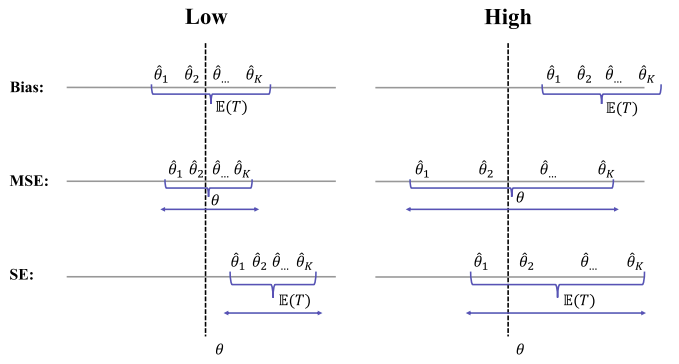
\includegraphics[
        width=0.7\linewidth,
        height=6cm,
        keepaspectratio,
    ]{images/statistics/bias-se-mse-visual.png}
    \caption{Visual Representation of Bias, MSE and SE}
\end{figure}


\subsection{Bias}\label{Sampling Plans/Measures of closeness/Bias}

\hfill
$
    bias
    = \dParenBrac{\dsum_{k=1}^{K} \hat{\theta}_k \pi_k} - \theta
    = \mathbb{E}(T) - \theta
$
\hfill \cite{statistics/book/Statistics-for-Data-Scientists/Maurits-Kaptein}

\vspace{0.5cm}

\begin{enumerate}
    \item The bias is the difference between the weighted average - over all possible $K$ samples - of the sample estimate $\hat{\theta}_k$'s and the true population parameter $\theta$.
    \hfill \cite{statistics/book/Statistics-for-Data-Scientists/Maurits-Kaptein}

    \item The weights in this weighted average are provided by the probabilities $\pi_k$.
    \hfill \cite{statistics/book/Statistics-for-Data-Scientists/Maurits-Kaptein}

    \item  If the bias of an estimator is \textbf{zero}, this means that, if we repeatedly take samples using our sampling plan and repeatedly compute our statistic of interest, the average over all of those statistics is equal to the true population parameter.
    \hfill \cite{statistics/book/Statistics-for-Data-Scientists/Maurits-Kaptein}
    \\
    If the bias is \textbf{zero}, the estimator, under the sampling plan that is being evaluated, is said to be \textbf{unbiased}.
    \hfill \cite{statistics/book/Statistics-for-Data-Scientists/Maurits-Kaptein}

    \item The bias of an estimator is thus the difference between this estimator’s expected value and the true population value.
    \hfill \cite{statistics/book/Statistics-for-Data-Scientists/Maurits-Kaptein}

    \item A small bias of an estimator under a sampling plan does \textbf{not} guarantee that individual sample results $\hat{\theta}_k$ are actually close to the population parameter $\theta$; it just states that they are close on average, if we were to sample over and over again.
    \hfill \cite{statistics/book/Statistics-for-Data-Scientists/Maurits-Kaptein}

    \item If the bias is small, $\mathbb{E}(T)$ is close to the parameter value $\theta$.\\
    If the bias is large, $\mathbb{E}(T)$ is \textbf{not} close to $\theta$
    \hfill \cite{statistics/book/Statistics-for-Data-Scientists/Maurits-Kaptein}

    \item If the sampling plan is unbiased and thus $\mathbb{E}(T) = \theta$, the RMSE and the SE are identical.
    \hfill \cite{statistics/book/Statistics-for-Data-Scientists/Maurits-Kaptein}


\end{enumerate}









\subsection{Mean Square Error (MSE)}\label{Sampling Plans/Measures of closeness/Mean Square Error (MSE)}

\hfill
$
    MSE
    = \dsum_{k=1}^{K} \dParenBrac{\hat{\theta}_k - \theta}^2 \pi_k
$
\hfill \cite{statistics/book/Statistics-for-Data-Scientists/Maurits-Kaptein}


\begin{enumerate}
    \item To capture the variability in the sample results $\hat{\theta}_1, \hat{\theta}_2,..., \hat{\theta}_K$ with respect to the true value $\theta$, we use the so-called mean squared error (MSE).
    \hfill \cite{statistics/book/Statistics-for-Data-Scientists/Maurits-Kaptein}

    \item The MSE measures the weighted average squared distance of the sample results $\hat{\theta}_1, \hat{\theta}_2,..., \hat{\theta}_K$ from the population parameter $\theta$.
    \hfill \cite{statistics/book/Statistics-for-Data-Scientists/Maurits-Kaptein}

    \item The weights are determined by the sampling probabilities.
    \hfill \cite{statistics/book/Statistics-for-Data-Scientists/Maurits-Kaptein}

    \item The smaller the MSE the better the sampling plan.
    \hfill \cite{statistics/book/Statistics-for-Data-Scientists/Maurits-Kaptein}

    \item If the MSE is small, the variability of the $\hat{\theta}_k$'s around $\theta$ is small, \\
    while if the MSE is large, the variability around $\theta$ is large.
    \hfill \cite{statistics/book/Statistics-for-Data-Scientists/Maurits-Kaptein}
\end{enumerate}







\subsection{Root Mean Square Error (RMSE)}\label{Sampling Plans/Measures of closeness/Root Mean Square Error (RMSE)}


\hfill
$
    RMSE
    = \sqrt{MSE}
    = \sqrt{{SE}^2 + \dParenBrac{\mathbb{E}(T) - \theta}^2}
$
\hfill \cite{statistics/book/Statistics-for-Data-Scientists/Maurits-Kaptein}






\subsection{Standard Error (SE)}\label{Sampling Plans/Measures of closeness/Standard Error (SE)}


\hfill
$
    SE = \sqrt{
        \dsum_{k=1}^{K} \dParenBrac{
            \hat{\theta}_k - \mathbb{E}(T)
        }^2
        \pi_k
    }
$
\hfill \cite{statistics/book/Statistics-for-Data-Scientists/Maurits-Kaptein}


\begin{enumerate}
    \item It represents the variability of the sampling plan with respect to the expected population parameter $\mathbb{E}(T)$ instead of using the true population parameter $\theta$.
    \hfill \cite{statistics/book/Statistics-for-Data-Scientists/Maurits-Kaptein}

    \item Standard error of an estimator is used as a measure to represent our uncertainty regarding an estimate.
    \hfill \cite{statistics/book/Statistics-for-Data-Scientists/Maurits-Kaptein}

    \item If the SE is small, the variability of the $\hat{\theta}_k$’s around $\mathbb{E}(T)$ is small.
    \hfill \cite{statistics/book/Statistics-for-Data-Scientists/Maurits-Kaptein}

    \item $SE(cT ) = c\ SE(T) \hspace{2cm} \forall\  c \in \mbbR$
    \hfill \cite{statistics/book/Statistics-for-Data-Scientists/Maurits-Kaptein}
\end{enumerate}








\section{Types of Samplings}

\begin{enumerate}

\item \textbf{Non-representative Sampling} \label{Sampling Plans/Non-representative Sampling}
\hfill \cite{statistics/book/Statistics-for-Data-Scientists/Maurits-Kaptein}

    \begin{enumerate}
        \item Although these sampling methods are frequently in use, it is strongly recommended not to apply these methods, unless knowledge is available on how to adjust or correct the sample for inferential purposes.
        \hfill \cite{statistics/book/Statistics-for-Data-Scientists/Maurits-Kaptein}

        \item These have the risk that some units are much more likely to be included in the sample than others, which can make statistics computed on the sample data bad estimates for the population parameters of interest.
        \hfill \cite{statistics/book/Statistics-for-Data-Scientists/Maurits-Kaptein}

        \item With non-representative sampling some units are not only more likely to be included in the sample, we also do not actually know how likely units were included.
        \hfill \cite{statistics/book/Statistics-for-Data-Scientists/Maurits-Kaptein}

        \item Even if we wanted to, we could not control for these systematic differences between units.
        \hfill \cite{statistics/book/Statistics-for-Data-Scientists/Maurits-Kaptein}
    \end{enumerate}

    \vspace{0.2cm}
    \textbf{SEE}:
    \begin{enumerate}
        \item \fullref{Sampling Plans/Non-representative Sampling/Convenience Sampling}
        \item \fullref{Sampling Plans/Non-representative Sampling/Haphazard Sampling}
        \item \fullref{Sampling Plans/Non-representative Sampling/Purposive Sampling or Judgmental Sampling}
    \end{enumerate}


\item \textbf{Representative Sampling} \label{Sampling Plans/Representative Sampling}
\hfill \cite{statistics/book/Statistics-for-Data-Scientists/Maurits-Kaptein}
    \begin{enumerate}
        \item We sample units in such a way that we do know how likely units are to be included in the sample (even if they will be different from unit to unit).
        \hfill \cite{statistics/book/Statistics-for-Data-Scientists/Maurits-Kaptein}

        \item Random sampling is a sampling method that uses a random mechanism.
        \hfill \cite{statistics/book/Statistics-for-Data-Scientists/Maurits-Kaptein}

        \begin{enumerate}
            \item The probability of each unit in the population of becoming part of the sample is both positive and known.
            \hfill \cite{statistics/book/Statistics-for-Data-Scientists/Maurits-Kaptein}
        \end{enumerate}
    \end{enumerate}

    \vspace{0.2cm}
    \textbf{SEE}:
    \begin{enumerate}
        \item \fullref{Sampling Plans/Representative Sampling/Simple Random Sampling}
        \item \fullref{Sampling Plans/Representative Sampling/Systematic Sampling}
        \item \fullref{Sampling Plans/Representative Sampling/Stratified Sampling}
        \item \fullref{Sampling Plans/Representative Sampling/Cluster Sampling}
    \end{enumerate}
\end{enumerate}

\clearpage
\section{Convenience Sampling \cite{statistics/book/Statistics-for-Data-Scientists/Maurits-Kaptein}}\label{Sampling Plans/Non-representative Sampling/Convenience Sampling}

\begin{enumerate}
    \item Convenience sampling collects only units from the population that can be easily obtained.
    \hfill \cite{statistics/book/Statistics-for-Data-Scientists/Maurits-Kaptein}

    \item This may provide a biased sample, as it represents only one small part or time window of the whole processing window for a batch of products. The term \textbf{bias}\label{Sampling Plans/Non-representative Sampling/Convenience Sampling/bias} indicates that we obtain the value of interest with a systematic mistake.
    \hfill \cite{statistics/book/Statistics-for-Data-Scientists/Maurits-Kaptein}

    \item  Convenience sampling is often justified by using the argument of population homogeneity. This insinuates that either the population units are not truly different or the process produces the population of units in random order. 
    \hfill \cite{statistics/book/Statistics-for-Data-Scientists/Maurits-Kaptein}
\end{enumerate}


\section{Haphazard Sampling \cite{statistics/book/Statistics-for-Data-Scientists/Maurits-Kaptein}}\label{Sampling Plans/Non-representative Sampling/Haphazard Sampling}

\begin{enumerate}
    \item Haphazard sampling is often believed to be an excellent way of collecting samples, because it gives a feeling or the impression that each unit was collected completely at random.
    \hfill \cite{statistics/book/Statistics-for-Data-Scientists/Maurits-Kaptein}

    \item Despite the feeling of randomness when performing haphazard sampling, often the resulting sample is not truly random.
    \hfill \cite{statistics/book/Statistics-for-Data-Scientists/Maurits-Kaptein}
\end{enumerate}

\section{Purposive Sampling/ Judgmental Sampling \cite{statistics/book/Statistics-for-Data-Scientists/Maurits-Kaptein}}\label{Sampling Plans/Non-representative Sampling/Purposive Sampling or Judgmental Sampling}

\begin{enumerate}
    \item Purposive sampling or judgmental sampling tries to sample units for a specific purpose.
    \hfill \cite{statistics/book/Statistics-for-Data-Scientists/Maurits-Kaptein}

    \item This means that the collection of units is focused on one or more particular characteristics and hence it implies that only units that are more alike are sampled.
    \hfill \cite{statistics/book/Statistics-for-Data-Scientists/Maurits-Kaptein}

    \item This way of sampling is strongly related to the definition of the population, since deliberately excluding units from the sample is analogous to limiting the population of interest.
    \hfill \cite{statistics/book/Statistics-for-Data-Scientists/Maurits-Kaptein}

    \item Purposive sampling may be useful, but it is limited since it does not allow us in general to make statements about the whole population, and at best only about a limited part of the population (although we may not be sure either).
    \hfill \cite{statistics/book/Statistics-for-Data-Scientists/Maurits-Kaptein}

    \item It does most likely produce a biased sample with respect to the complete population.
    \hfill \cite{statistics/book/Statistics-for-Data-Scientists/Maurits-Kaptein}
\end{enumerate}


\clearpage
\section{Simple Random Sampling \cite{statistics/book/Statistics-for-Data-Scientists/Maurits-Kaptein}}\label{Sampling Plans/Representative Sampling/Simple Random Sampling}

\begin{table}[H]
    \centering
    \begin{tabular}{l l}
        $N$ & population size \\
        $n$ & sample size \\
        $K$ & number of possible samples \\
        $k$ & sample index ($ k \in \dParenBrac{1,\cdots,K}$) \\
        $S_k$ & sample\\
    \end{tabular}
\end{table}

\begin{enumerate}
    \item Implicitly assume that there is no particular group structure present in the population.
    \hfill \cite{statistics/book/Statistics-for-Data-Scientists/Maurits-Kaptein}

    \item Simple random sampling is a way of collecting samples such that each unit from the population has the exact same probability of becoming part of the sample.
    \hfill \cite{statistics/book/Statistics-for-Data-Scientists/Maurits-Kaptein}


    \item Simple random sampling is a conceptually easy method of forming random samples but it can prove hard in practice.
    \hfill \cite{statistics/book/Statistics-for-Data-Scientists/Maurits-Kaptein}

    \item Simple random sampling is frequently combined with other choices or settings (see stratified and cluster sampling).
    \hfill \cite{statistics/book/Statistics-for-Data-Scientists/Maurits-Kaptein}

    \item Number of unique samples $
        = K
        = \dfrac{N!}{n!(N-n)!}
    $
    \hfill \cite{statistics/book/Statistics-for-Data-Scientists/Maurits-Kaptein}

    \item the probability of collecting sample $S_k$, using sequential sampling $
        = \dfrac{1}{K}
        = \dfrac{n!(N-n)!}{N!}
    $
    \hfill \cite{statistics/book/Statistics-for-Data-Scientists/Maurits-Kaptein}

    \item The probability that a specific unit is part of the sample $
        = \dfrac{n}{N}
    $
    \hfill \cite{statistics/book/Statistics-for-Data-Scientists/Maurits-Kaptein}

    \item The probability that a specific unit is \textbf{not} contained in the sample $
        = 1 - \dfrac{n}{N}
        = \dfrac{N-n}{N}
    $
    \hfill \cite{statistics/book/Statistics-for-Data-Scientists/Maurits-Kaptein}

    \item The number of samples that does \textbf{not} contain a specific unit $
        = \dfrac{(N - 1)!}{n!(N - 1 - n)!}
    $
    \hfill \cite{statistics/book/Statistics-for-Data-Scientists/Maurits-Kaptein}

    \item Number of samples that contain certain unit $i$ = $\dfrac{nK}{N}$
    \hfill \cite{statistics/book/Statistics-for-Data-Scientists/Maurits-Kaptein}
    \\
    $
        \Rightarrow
        \dsum_{k=1}^{K}\ \dsum_{i \in S_k} x_i
        = \dfrac{nK}{N}\dsum_{i=1}^{N} x_i
    $
    \hfill \cite{statistics/book/Statistics-for-Data-Scientists/Maurits-Kaptein}

    \item Population Variance: $
        \sigma^2
        = \dfrac{1}{N} \dsum_{i=1}^N (x_i-\mu)^2
    $
    \hfill \cite{statistics/book/Statistics-for-Data-Scientists/Maurits-Kaptein}

    \item \textbf{Disadvantage}: When the numbers of units across these subpopulations are (substantially) different, simple random may not collect units from each subgroup.
    \hfill \cite{statistics/book/Statistics-for-Data-Scientists/Maurits-Kaptein}

\end{enumerate}

\vspace{0.5cm}
\textbf{Example}:
\begin{enumerate}
    \item[] $N = 20,\ n = 5$

    \item[] $K = \dfrac{20!}{5!\cdot 15!}=15504$


\end{enumerate}


\subsection{Estimation for population mean}
\begin{enumerate}
    \item Estimator: $
        T
        = \bar{x}
        = \dfrac{1}{n} \dsum_{i=1}^n x_i
    $
    \hfill \cite{statistics/book/Statistics-for-Data-Scientists/Maurits-Kaptein}

    \item Bias: $0$
    \hfill \cite{statistics/book/Statistics-for-Data-Scientists/Maurits-Kaptein}

    \item $
        MSE(\bar{x}_k)
        = \dfrac{\sigma^2 }{n}
        \dParenBrac{\dfrac{N}{N-1}}
        \dParenBrac{1-\dfrac{n}{N}}
        = \dfrac{\sigma^2\ (N-n)}{n\ (N-1)}
    $
    \hfill \cite{statistics/book/Statistics-for-Data-Scientists/Maurits-Kaptein}
    \\
    MSE shows that it becomes equal to zero when the sample size $n$ becomes equal to the population size $N$.
    \hfill \cite{statistics/book/Statistics-for-Data-Scientists/Maurits-Kaptein}
    \\
    The MSE will not become zero when the estimator is biased, even if the sample size is equal to the population size.
    \hfill \cite{statistics/book/Statistics-for-Data-Scientists/Maurits-Kaptein}


    \item $
        \mathbb{E}[T]
        = \dfrac{1}{K}\dsum_{k=1}^{K} \bar{x}_k
        = \dfrac{1}{nK}\dsum_{k=1}^{K}\ \dsum_{i \in S_k} x_i
        = \dfrac{1}{N}\dsum_{i=1}^{N} x_i
        = \mu
    $
    \hfill \cite{statistics/book/Statistics-for-Data-Scientists/Maurits-Kaptein}
\end{enumerate}


\subsection{Estimation of the sample MSE}

\begin{enumerate}
    \item unbiased estimator for $\sigma^2$: \\
    $
       \hat{\sigma}^2 = \dfrac{N - 1}{N}\ s^2_k
    $
    \hfill
    $
        \dParenBrac{\
            s^2_k = \dfrac{1}{n - 1} \dsum_{i\ \in\ S_k} (x_i - \bar{x}_k )^2
        \ }
    $
    \hfill \cite{statistics/book/Statistics-for-Data-Scientists/Maurits-Kaptein}

    \item $
        \hat{MSE}(\bar{x}_k)
        = \dfrac{N - n}{N n}\ s^2_k
    $
    \hfill \cite{statistics/book/Statistics-for-Data-Scientists/Maurits-Kaptein}

    \item This is an unbiased estimator of the MSE of the arithmetic average in $MSE(\bar{x}_k)$ and it may also be used when the observations are binary.
    \hfill \cite{statistics/book/Statistics-for-Data-Scientists/Maurits-Kaptein}


\end{enumerate}




\subsection{Sample Statistics ($T_n$)}

\begin{enumerate}
    \item We can view a sample $X_1 , X_2 , \cdots, X _n$ of size $n$ from a population as a set of random variables (and $x_1 , x_2, \cdots , x _n$ as the set of realizations) all coming from the same distribution function $F$.
    Let $X_1 , X_2, \cdots , X _n$ be i.i.d. with $X _i \sim F$
    \hfill \cite{statistics/book/Statistics-for-Data-Scientists/Maurits-Kaptein}

    \item A sample statistic $T_n \in \mbbR$ is now defined as any function $T_n \equiv T (X_1, X_2, \cdots , X _n )$ that is applied to the sample $X_1 , X_2, \cdots , X _n$.
    As $T_n$ is a function of random variables, it is itself a random variable.
    \hfill \cite{statistics/book/Statistics-for-Data-Scientists/Maurits-Kaptein}

    \item realization for the sample statistic $T_n$: $t _n = T (x_1, x_2, \cdots , x _n )$
    \hfill \cite{statistics/book/Statistics-for-Data-Scientists/Maurits-Kaptein}

    \item \textbf{Sample average}: $T_n = \bar{X} = \dfrac{1}{n}\dsum^n _{i=1} X _i$
    \hfill \cite{statistics/book/Statistics-for-Data-Scientists/Maurits-Kaptein}

    \item \textbf{Sample variance}: $T_n = S^2 = \dfrac{1}{n - 1} \dsum^n _{i=1}(X _i - \bar{X})^2$
    \hfill \cite{statistics/book/Statistics-for-Data-Scientists/Maurits-Kaptein}

    \item \textbf{Sample standard deviation}: $T_n = S^2 = \sqrt{\dfrac{1}{n - 1} \dsum^n _{i=1}(X _i - \bar{X})^2}$
    \hfill \cite{statistics/book/Statistics-for-Data-Scientists/Maurits-Kaptein}

    \item \textbf{Sample skewness}: $T_n = b_1 = \dfrac{1}{n S^3} \dsum^n _{i=1} (X _i - \bar{X})^3$
    \hfill \cite{statistics/book/Statistics-for-Data-Scientists/Maurits-Kaptein}

    \item \textbf{Sample excess kurtosis}: $T_n = b_2 = \dParenBrac{\dfrac{1}{n S^4} \dsum^n _{i=1} (X _i - \bar{X})^4} - 3$
    \hfill \cite{statistics/book/Statistics-for-Data-Scientists/Maurits-Kaptein}

    \item \textbf{Sample minimum}: $T_n = X_{(1)} = \min \dCurlyBrac{X_1, X_2, \cdots, X _n }$
    \hfill \cite{statistics/book/Statistics-for-Data-Scientists/Maurits-Kaptein}

    \item \textbf{Sample maximum}: $T_n = X_{(n)} = \max \dCurlyBrac{X_1, X_2, \cdots, X _n }$
    \hfill \cite{statistics/book/Statistics-for-Data-Scientists/Maurits-Kaptein}

    \item \textbf{quantile}:
    \begin{enumerate}
        \item If $np \in \mathbb{N}$ is an integer, the quantile $x _p$ is estimated by the average of two sequential order statistics: $q _p = \dfrac{[X_{(np)} + X_{(1+np)}]}{2}$.
        \hfill \cite{statistics/book/Statistics-for-Data-Scientists/Maurits-Kaptein}

        \item If $np \notin \mathbb{N}$ is not an integer, we take the smallest integer value that is larger than or equal to $np$, which is denoted by $\dceil{np}$.
        \hfill \cite{statistics/book/Statistics-for-Data-Scientists/Maurits-Kaptein}
    \end{enumerate}
\end{enumerate}




\clearpage
\section{Systematic Sampling \cite{statistics/book/Statistics-for-Data-Scientists/Maurits-Kaptein}}\label{Sampling Plans/Representative Sampling/Systematic Sampling}

\begin{table}[H]
    \centering
    \begin{tabular}{l l l}
        $N$ & population size & $N=nm$\\
        $n$ & number of groups & = sample size \\
        $m$ & number of units in each group & = number of possible samples\\
        $k$ & sample index & $k \in \dParenBrac{1,\cdots,m}$ \\
        $S_k$ & sample & \\
    \end{tabular}
\end{table}

\begin{enumerate}
    \item Implicitly assume that there is no particular group structure present in the population.
    \hfill \cite{statistics/book/Statistics-for-Data-Scientists/Maurits-Kaptein}

    \item Steps:
    \hfill \cite{statistics/book/Statistics-for-Data-Scientists/Maurits-Kaptein}
    \begin{enumerate}
        \item First the population should be divided into $n$ groups and the order of the units (if Some order exists) should be maintained (or otherwise fix the order).\\
        Each group consists of $m$ units ordered from $1$ to $m$ in each group.

        \item Collect $p$th unit ($p \in \dParenBrac{1,\cdots,m}$) from all $n$ groups with probability of $\dfrac{1}{m}$\\
        (each unit in the population still has the same probability of being collected)\\
        $S_k = \dCurlyBrac{k, k + m, k + 2m, \cdots , k + (n - 1)m}$ 
        \hfill
        (Total units collected $= n$) 
        \hfill \cite{statistics/book/Statistics-for-Data-Scientists/Maurits-Kaptein} \\
        So, total number of samples $= m$ only

    \end{enumerate}

    \item The possible samples from systematic sampling are quite different from the set of samples that can be obtained with simple random sampling.
    \hfill \cite{statistics/book/Statistics-for-Data-Scientists/Maurits-Kaptein}

    \item population mean: $
        \mu 
        = \dfrac{1}{N}\ \dsum^m_{h=1} \ \dsum^n_{i=1} x_{\ k+m(i-1)}
    $
    \hfill \cite{statistics/book/Statistics-for-Data-Scientists/Maurits-Kaptein}

    \item population variance: $
        \sigma^2 
        = \dfrac{1}{N}\ \dsum^m_{k=1} \ \dsum^n_{i=1} (x_{\ k+m(i-1)} - \mu)^2
    $
    \hfill \cite{statistics/book/Statistics-for-Data-Scientists/Maurits-Kaptein}
    
    \item sample average for sample $S_k$: $
        \bar{x}_k 
        = \dfrac{1}{n}\ \dsum^n_{i=1} x_{\ k+m(i-1)}
    $
    \hfill \cite{statistics/book/Statistics-for-Data-Scientists/Maurits-Kaptein}

    \item Systematic sampling can be more efficient than simple random sampling, in particular when the variance in the systematic samples is larger than the population variance (which is impossible to verify in practice).
    \hfill \cite{statistics/book/Statistics-for-Data-Scientists/Maurits-Kaptein}

    \item The most important \textbf{advantage} of systematic sampling over simple random sampling is the ease with which the sample may be collected.
    \hfill \cite{statistics/book/Statistics-for-Data-Scientists/Maurits-Kaptein}

    \item A clear \textbf{disadvantage} of systematic sampling is that the “period” for systematic sampling may coincide with particular patterns in the process or population.
    \hfill \cite{statistics/book/Statistics-for-Data-Scientists/Maurits-Kaptein}

    \item \textbf{Disadvantage}: When the numbers of units across these subpopulations are (substantially) different, systematic sampling may not collect units from each subgroup.
    \hfill \cite{statistics/book/Statistics-for-Data-Scientists/Maurits-Kaptein}

    \item TODO? Systematic Sampling samples ($S_1,\cdots,S_m$) are subset of Simple Random Sampling samples ($S_1,\cdots,S_K$).
\end{enumerate}

\vspace{0.5cm}
\textbf{Example}:
\begin{enumerate}
    \item[] $N = 20,\ n = 5$

    \item[] $m = \dfrac{20}{5}=4$

    
\end{enumerate}



\subsection{Estimation for population mean}
\begin{enumerate}
    \item Estimator: $
        \dfrac{1}{n} \dsum_{i=1}^n x_i
    $
    \hfill \cite{statistics/book/Statistics-for-Data-Scientists/Maurits-Kaptein}
    \\
    if population can be perfectly split up into $n$ groups of $m$ units:\\
    Unbiased Estimator: $\bar{x}_k$
    
    \item Bias: $0$
    \hfill \cite{statistics/book/Statistics-for-Data-Scientists/Maurits-Kaptein}

    \item MSE: $
        \sigma^2 -
        \dfrac{1}{N}
        \dsum_{h=1}^{n}
        \dsum_{i=1}^{m}
        (x_{h+m(i-1)} - \bar{x}_h)^2
    $
    \hfill \cite{statistics/book/Statistics-for-Data-Scientists/Maurits-Kaptein}

\end{enumerate}



\subsection{Estimation of the MSE}

\begin{enumerate}
    \item In the general setting for systematic sampling, an unbiased estimation of the MSE is \textbf{not possible}.
    \hfill \cite{statistics/book/Statistics-for-Data-Scientists/Maurits-Kaptein}

    \item Given that there is no systematic difference between units based on their position in the groups (and the ratio of sample and population size is an integer), the MSE of the sample average under systematic sampling becomes equal to the MSE of the sample average under simple random sampling.
    \hfill \cite{statistics/book/Statistics-for-Data-Scientists/Maurits-Kaptein}
    
    \item unbiased estimator: $
        \dfrac{N - 1}{N}\ s^2_k
    $
    \hfill
    $
        s^2_k = \dfrac{1}{n - 1} \dsum^n_{i=1} (x_{k+m(i-1)} - \bar{x}_k )^2
    $
    \hfill \cite{statistics/book/Statistics-for-Data-Scientists/Maurits-Kaptein}
\end{enumerate}






\clearpage
\section{Stratified Sampling \cite{statistics/book/Statistics-for-Data-Scientists/Maurits-Kaptein}}\label{Sampling Plans/Representative Sampling/Stratified Sampling}

\begin{customArrayStretch}{1.3}
\begin{longtable}{>{\centering\arraybackslash}p{1.5cm} p{9cm} p{3.5cm}}

\hline\endfirsthead
\hline\endhead
\hline\endfoot
\hline\endlastfoot

$N$ & total population size & \\ \hline

$n$ & total sample size & \\ \hline

$M$ & number of sub-populations & \\ \hline

$N_h$ & $k$th sub-population size & $\tsum_{h=1}^{M} N_h = N$ \\ \hline

$n_h$ & sample size from $k$th sub-population & $\tsum_{h=1}^{M} n_h = n$ \\ \hline

$h$ & Stratum index & $h \in \dCurlyBrac{1, \cdots, M}$ \\ \hline

$k$ & Stratum index & $k \in \dCurlyBrac{1, \cdots, K_S}$ \\ \hline

$K_h$ & The number of possible samples that can be drawn from stratum $h$ \\ \hline

$K_S$ & total number of possible samples \\ \hline

$(h, i)$ & index of unit & \begin{minipage}{3.2cm}
    \vspace{0.1cm}
    $i \in \dCurlyBrac{1, 2,\cdots, N_h }$ \\
    and $h \in \dCurlyBrac{1, 2,..., M}$
    \vspace{0.1cm}
\end{minipage}  \\ \hline

$x_{hi}$ & unit $i$ in stratum $h$ \\ \hline

$w_{h}$ &
    weight of strata $h$ while sampling &
    \begin{minipage}{3.2cm}
        \vspace{0.1cm}
        $w_{h} = \dfrac{N_h}{N}$
        \vspace{0.1cm}
    \end{minipage}
    \\ \hline

$f_{h}$ &
    sample fraction in stratum $h$ &
    \begin{minipage}{3.2cm}
        \vspace{0.1cm}
        $f_{h} = \dfrac{n_h}{N_h}$
        \vspace{0.1cm}
    \end{minipage}
    \\ \hline

$S_{h,k}$ &
\multicolumn{2}{l}{
    \begin{minipage}{11cm}
        \vspace{0.1cm}
        $S_{h,k}$ is the collected sample in stratum $h$ \\
        The $k$-th possible sample from stratum $h$ \\
        (e.g., $S_{2,3}$ is the $3$rd possible sample from stratum $2$) \\
        focuses on one stratum
        \vspace{0.1cm}
    \end{minipage}
} \\ \hline

$S_k$ &
\multicolumn{2}{l}{
    \begin{minipage}{11cm}
        \vspace{0.1cm}
        The $k$-th possible full stratified sample (i.e., across all strata). \\
        Each $S_k$ includes one selected sample from each stratum.\\
        focuses on a complete sample (all strata combined)
        \vspace{0.1cm}
    \end{minipage}
} \\ \hline

\end{longtable}
\end{customArrayStretch}

\begin{enumerate}
    \item Stratified sampling is used to accommodate the issue of missing out on sub-populations during sampling by setting the sample size for each subpopulation (often called \textbf{strata}\label{Sampling Plans/Representative Sampling/Stratified Sampling/strata}) to a fixed percentage of the number of units of the subpopulation.
    \hfill \cite{statistics/book/Statistics-for-Data-Scientists/Maurits-Kaptein}

    \item Steps:
    \hfill \cite{statistics/book/Statistics-for-Data-Scientists/Maurits-Kaptein}
    \begin{enumerate}
        \item The population is then divided into $n$ groups such that the order in units is maintained.

        \item From $k$th group/ strata one unit is randomly collected with probability $\dfrac{n_h}{N_h}$, when each group contains $n_h$ units.\\
        Unlike systematic sampling, random unit is collected instead of $p$th unit.
    \end{enumerate}

    \item This form of stratified sampling is not identical to systematic sampling (although this method of stratified sampling is sometimes referred to as systematic sampling).
    \hfill \cite{statistics/book/Statistics-for-Data-Scientists/Maurits-Kaptein}

    \item Stratified sampling may lead to samples that are not possible with systematic sampling, but it does not produce all possible samples from simple random sampling.
    \hfill \cite{statistics/book/Statistics-for-Data-Scientists/Maurits-Kaptein}

    \item $
        K_h = \binom{N_h}{n_h} = \dfrac{N_h!}{n_h!(N_h-n_h)!}
    $
    \hfill \cite{statistics/book/Statistics-for-Data-Scientists/Maurits-Kaptein}

    \item The number of possible samples: $
        K_S
        = \dprod_{h=1}^{M} \dfrac{N_h!}{n_h!(N_h-n_h)!}
        = \dprod_{h=1}^{M} K_h
    $
    \hfill \cite{statistics/book/Statistics-for-Data-Scientists/Maurits-Kaptein}

    \item The probability of collecting any of the $K_S$ samples $
        = \dfrac{1}{K_S}
    $
    \hfill \cite{statistics/book/Statistics-for-Data-Scientists/Maurits-Kaptein}

    \item The probability of collecting a unit now depends on the stratum the unit is part of.
    \hfill \cite{statistics/book/Statistics-for-Data-Scientists/Maurits-Kaptein}

    \item If $
        \dfrac{n_i}{N_i} = \dfrac{n_j}{N_j}
        \hspace{0.3cm}
        \forall
        \hspace{0.3cm}
        i,j \in \dParenBrac{1,\cdots,M}
    $, then its called \textbf{Proportional Stratified Sampling}.\label{Sampling Plans/Representative Sampling/Stratified Sampling/Proportional Stratified Sampling}
    \hfill \cite{statistics/book/Statistics-for-Data-Scientists/Maurits-Kaptein}

\end{enumerate}


\vspace{0.5cm}\hspace{0cm}
\textbf{Example}: sample $10\%$ from each sub-population


\subsection{population stratum}
\begin{enumerate}
    \item population stratum mean: $
        \mu_h = \dfrac{1}{N_h} \ \dsum_{i=1}^{N_h} \ x_{hi}
    $
    \hfill \cite{statistics/book/Statistics-for-Data-Scientists/Maurits-Kaptein}

    \item population stratum variance: $
        \sigma^2_h = \dfrac{1}{N_h} \ \dsum_{i=1}^{N_h} \ (x_{hi} - \mu_h)^2
    $
    \hfill \cite{statistics/book/Statistics-for-Data-Scientists/Maurits-Kaptein}

\end{enumerate}



\subsection{population}
\begin{enumerate}
    \item population mean: $
        \mu
        = \dfrac{1}{N} \ \dsum_{h=1}^M \ \dsum_{i=1}^n\  x_{hi}
        = \dsum_{h=1}^M \ w_h\mu_h
    $
    \hfill \cite{statistics/book/Statistics-for-Data-Scientists/Maurits-Kaptein}
    \begin{enumerate}
        \item $w_h = \dfrac{N_h}{N}$
        \hfill \cite{statistics/book/Statistics-for-Data-Scientists/Maurits-Kaptein}

        \item $\dsum_{h=1}^M \ w_h = 1$
        \hfill \cite{statistics/book/Statistics-for-Data-Scientists/Maurits-Kaptein}
    \end{enumerate}


    \item population variance: $
        \sigma^2
        \equiv \dfrac{1}{N} \ \dsum_{h=1}^M \ \dsum_{i=1}^{N_h} (x_{hi} - \mu)^2
        = \dsum_{h=1}^M w_h \sigma_h^2 + \dsum_{h=1}^M w_h (\mu_h - \mu)^2
    $
    \hfill \cite{statistics/book/Statistics-for-Data-Scientists/Maurits-Kaptein}
    \vspace{0.15cm}
    \begin{enumerate}
        \item \textbf{within (strata) variances}: the first part represents a weighted mean of the within strata variances

        \item \textbf{between (strata) variances}: the second part represents a weighted mean of the squared distances of the strata means to the population mean
    \end{enumerate}

\end{enumerate}


\subsubsection{Estimation for population mean}
\begin{enumerate}
    \item Estimator: $
        \dsum_{h=1}^{M}
        \dfrac{N_h}{N}
        \dParenBrac{\dfrac{1}{n_h} \dsum_{i=1}^{n_h} x_{hi}}
        =
        \dsum_{h=1}^{M} \ w_h \ \bar{x}_{h,k}
    $
    \hfill \cite{statistics/book/Statistics-for-Data-Scientists/Maurits-Kaptein}

    \item Bias: $0$
    \hfill \cite{statistics/book/Statistics-for-Data-Scientists/Maurits-Kaptein}

    \item MSE: $
        \dsum_{h=1}^{M}
        \dSquareBrac{
            \dParenBrac{
                \dfrac{
                    N_h^2\ (N_h - n_h)
                }{
                    n_h\ (N_h-1)\ N^2
                }
            } \sigma_h^2
        }
    $
    \hfill \cite{statistics/book/Statistics-for-Data-Scientists/Maurits-Kaptein}
\end{enumerate}




\subsection{sample stratum}
\begin{enumerate}
    \item sample stratum mean: $
        \bar{x}_{h,k} = \dfrac{1}{n_h} \ \dsum_{i \ \in \ S_{h,k}} \ x_{hi}
    $
    \hfill \cite{statistics/book/Statistics-for-Data-Scientists/Maurits-Kaptein}

    \item sample stratum variance: $
        s^2_{h,k} = \dfrac{1}{n_h-1} \ \dsum_{i \ \in \ S_{h,k}} \ (x_{hi} - \bar{x}_{h,k})^2
    $
    \hfill \cite{statistics/book/Statistics-for-Data-Scientists/Maurits-Kaptein}

    \item MSE for unbiased estimator:
    $
        MSE(\bar{x}_{h,k}) = \tVar[\bar{x}_{h,k}] = SE^2(\bar{x}_{h,k})
    $
    \hfill \cite{common/online/chatgpt}

    \item The bias and standard error within each stratum $h$ now follow the theory of simple random sampling.
    \hfill \cite{statistics/book/Statistics-for-Data-Scientists/Maurits-Kaptein}

    \item bias of $\bar{x}_{h,k}$ = 0 in stratum $h$ is zero for the stratum mean $\mu_h$

\end{enumerate}


\subsubsection{Estimation for sample stratum SE}
\begin{enumerate}
    \item $
        \hat{SE}(\bar{x}_{h,k})
        = \sqrt{\dfrac{1 - f_h}{n_h}} s_{h,k}
    $
    \hfill
    $f_h = \dfrac{n_h}{N_h}$
    \hfill \cite{statistics/book/Statistics-for-Data-Scientists/Maurits-Kaptein}
\end{enumerate}



\subsection{sample}
\begin{enumerate}
    \item Sample average: $
        \bar{x}_k = \dsum^M_{h=1} w_h\ \bar{x}_{h,k}
    $
    \hfill \cite{statistics/book/Statistics-for-Data-Scientists/Maurits-Kaptein}

    \item the \textit{simple random samples} from the different strata are completely \textbf{unrelated}, which implies that the sum of the squared standard errors of $w_h \ \bar{x}_{h,k}$ form the squared standard error of the sample average $\bar{x}_k$.
    \hfill \cite{statistics/book/Statistics-for-Data-Scientists/Maurits-Kaptein}
    \\
    $
        \tVar[\bar{x}_k] = \dsum_{h=1}^M w_h^2 \cdot \tVar[\bar{x}_{h,k}]
    $
    \hfill \cite{common/online/chatgpt}


    \item squared standard error of $\bar{x}_k$:
    $
        SE^2(\bar{x}_k) = \dsum_{h=1}^M w_h^2 \cdot SE^2(\bar{x}_{h,k})
    $
    \hfill \cite{common/online/chatgpt}

    \item $
        MSE(\bar{x}_k )
        = \dsum^M_{h=1} w^2_h \cdot MSE(\bar{x}_{h,k} )
        = \dsum^M_{h=1} \dfrac{N_h}{(N_h - 1)n_h} \ (1 - f_h)\ w^2_h\ \sigma^2_h$
    \hfill \cite{statistics/book/Statistics-for-Data-Scientists/Maurits-Kaptein}

\end{enumerate}


\subsubsection{Estimation of the sample MSE}

$
    \hat{MSE} (\bar{x}_k )
    = \dsum^M_{h=1} \dfrac{1 - f_h}{n_h} \ w^2_h\ s^2_{h,k}.
$
\hfill \cite{statistics/book/Statistics-for-Data-Scientists/Maurits-Kaptein}

SEE: \url{https://chatgpt.com/share/680251af-c100-800a-a533-c26a0001b651}

\subsubsection{Estimation of the sample SE}

An estimate of the standard error of $\bar{x}_k$ is now obtained by taking the square root of
the estimated MSE:
\hfill \cite{statistics/book/Statistics-for-Data-Scientists/Maurits-Kaptein}
\\
$
    \hat{SE}(\bar{x}_k) = \sqrt{\hat{MSE} (\bar{x}_k )}
$














\clearpage
\section{Cluster Sampling \cite{statistics/book/Statistics-for-Data-Scientists/Maurits-Kaptein}}\label{Sampling Plans/Representative Sampling/Cluster Sampling}

\begin{enumerate}[itemsep=0.2cm]
    \item Cluster sampling involves random sampling of groups or clusters of units in the population.
    \hfill \cite{statistics/book/Statistics-for-Data-Scientists/Maurits-Kaptein}

    \item Cluster sampling can be less representative than sampling units directly.
    \hfill \cite{statistics/book/Statistics-for-Data-Scientists/Maurits-Kaptein}

    \item Cluster sampling introduces a specific structure in the sample which should also be addressed when the data is being analyzed. 
    \hfill \cite{statistics/book/Statistics-for-Data-Scientists/Maurits-Kaptein}
    
    \item The cluster structure introduces two sources of variation in the data being collected. These sources of variation need to be quantified to make proper statements on the population of interest.
    \hfill \cite{statistics/book/Statistics-for-Data-Scientists/Maurits-Kaptein}
    \begin{enumerate}[itemsep=0.1cm]
        \item \textbf{Within-Cluster Variation}:\label{Sampling Plans/Representative Sampling/Cluster Sampling/Within-Cluster Variation}
        \hfill \cite{common/online/chatgpt}
        \begin{enumerate}
            \item This refers to the differences among units within the same cluster.
            \hfill \cite{common/online/chatgpt}

            \item This variation is often smaller compared to between-cluster variation because individuals within a cluster tend to be more similar.
            \hfill \cite{common/online/chatgpt}

        \end{enumerate}

        \item \textbf{Between-Cluster Variation}:\label{Sampling Plans/Representative Sampling/Cluster Sampling/Between-Cluster Variation}
        \hfill \cite{common/online/chatgpt}
        \begin{enumerate}
            \item This refers to the differences between clusters.
            \hfill \cite{common/online/chatgpt}

            \item This variation is often larger in cluster sampling because different clusters may have distinct characteristics.
            \hfill \cite{common/online/chatgpt}

        \end{enumerate}
        
    \end{enumerate}

    \item The sampling units for the \textit{first stage} are referred to as \textbf{primary cluster units}\label{Sampling Plans/Representative Sampling/Cluster Sampling/primary cluster units}.
    \hfill \cite{statistics/book/Statistics-for-Data-Scientists/Maurits-Kaptein}

    \item Sampling these different levels of clusters can be performed using simple random sampling, systematic sampling, or even stratified sampling, if certain cluster are put together on certain criteria.
    \hfill \cite{statistics/book/Statistics-for-Data-Scientists/Maurits-Kaptein}

    \item Cluster sampling is in a way related to stratified sampling (clusters may be viewed as strata).
    \hfill \cite{statistics/book/Statistics-for-Data-Scientists/Maurits-Kaptein}

    \item Since we deal with multiple levels of hierarchical clusters, the calculation of the probability of collecting one unit from the population and the probability of collecting one of the many sample sets are complex.
    \hfill \cite{statistics/book/Statistics-for-Data-Scientists/Maurits-Kaptein}
\end{enumerate}




\subsection{Single-Stage Cluster Sampling}\label{Sampling Plans/Representative Sampling/Cluster Sampling/Single-Stage Cluster Sampling}

A single-stage cluster sample uses a random sample of the clusters and then all units from these clusters are selected. 
\hfill \cite{statistics/book/Statistics-for-Data-Scientists/Maurits-Kaptein}

\subsubsection{cluster sizes are not all equal}
    
Estimator for population mean: $
    \dsum_{h=1}^{m}
    \dParenBrac{
        \dfrac{N_h}{
            \tsum_{h=1}^{m} N_h
        }
    }
    \bar{x}_h
$
\hfill \cite{statistics/book/Statistics-for-Data-Scientists/Maurits-Kaptein}

\begin{enumerate}[itemsep=0.25cm]
    \item Bias: $\geq 0$ (bias is close to zero but positive)
    \hfill \cite{statistics/book/Statistics-for-Data-Scientists/Maurits-Kaptein}

    \item MSE: $
        \sim 
        \dfrac{M^2}{m\ (M-1)\ N^2}
        \dParenBrac{1 - \dfrac{m}{M}}
        \dsum_{h=1}^M N_h^2\ (\mu_h - \mu)^2
    $
    \hfill \cite{statistics/book/Statistics-for-Data-Scientists/Maurits-Kaptein}
\end{enumerate}


\subsubsection{cluster sizes are all equal}

Estimator for population mean: $
    \dfrac{M}{m\ N}
    \dsum_{h=1}^{m}
    N_h \bar{x}_h
$
\hfill \cite{statistics/book/Statistics-for-Data-Scientists/Maurits-Kaptein}

\begin{enumerate}[itemsep=0.25cm]
    \item Bias: $0$
    \hfill \cite{statistics/book/Statistics-for-Data-Scientists/Maurits-Kaptein}

    \item MSE: $
        \dfrac{M^2}{m\ (M-1)\ N^2}
        \dParenBrac{1 - \dfrac{m}{M}}
        \dsum_{h=1}^M \dParenBrac{N_h\mu_h - \dfrac{N\mu}{M}}^2
    $
    \hfill \cite{statistics/book/Statistics-for-Data-Scientists/Maurits-Kaptein}
\end{enumerate}



\subsection{Two-Stage Cluster Sampling}\label{Sampling Plans/Representative Sampling/Cluster Sampling/Two-Stage Cluster Sampling}

In a two-stage cluster sample, the units from the sampled clusters are also randomly sampled instead of taking all units from the cluster.
\hfill \cite{statistics/book/Statistics-for-Data-Scientists/Maurits-Kaptein}

\subsubsection{cluster sizes are not all equal}
Estimator for population mean: $
    \dsum_{h=1}^{m}
    \dParenBrac{
        \dfrac{N_h}{
            \tsum_{h=1}^{m} N_h
        }
    }
    \bar{x}_h
$

\hfill \cite{statistics/book/Statistics-for-Data-Scientists/Maurits-Kaptein}
\begin{enumerate}[itemsep=0.25cm]
    \item Bias: $\geq 0$ (bias is close to zero but positive)
    \hfill \cite{statistics/book/Statistics-for-Data-Scientists/Maurits-Kaptein}

    \item MSE: $
        \sim 
        \dfrac{M}{m\ N^2}
        \dSquareBrac{
            \dParenBrac{1 - \dfrac{m}{M}}
            \dfrac{1}{M-1}
            \dsum_{h=1}^{M} N_h^2\ (\mu_h - \mu)^2
            + \dsum_{h=1}^{M} \dParenBrac{
                \dfrac{N_h^2\ (N_h-n_h)}{n_h\ (N_h-1)}
                \sigma_h^2
            }
        }
    $
    \hfill \cite{statistics/book/Statistics-for-Data-Scientists/Maurits-Kaptein}
\end{enumerate}


\subsubsection{cluster sizes are all equal}
Estimator for population mean: $
    \dfrac{M}{m\ N}
    \dsum_{h=1}^{m}
    N_h \bar{x}_h
$
\hfill \cite{statistics/book/Statistics-for-Data-Scientists/Maurits-Kaptein}

\begin{enumerate}[itemsep=0.25cm]
    \item Bias: $0$
    \hfill \cite{statistics/book/Statistics-for-Data-Scientists/Maurits-Kaptein}

    \item MSE: $
        \dfrac{M}{m\ N^2}
        \dSquareBrac{
            \dParenBrac{1 - \dfrac{m}{M}}
            \dfrac{1}{M-1}
            \dsum_{h=1}^{M} \dParenBrac{N_h\mu_h - \dfrac{N\mu}{M}}^2
            + \dsum_{h=1}^{M} \dParenBrac{
                \dfrac{N_h^2\ (N_h-n_h)}{n_h\ (N_h-1)}
            \sigma_h^2
            }
        }
    $
    \hfill \cite{statistics/book/Statistics-for-Data-Scientists/Maurits-Kaptein}
\end{enumerate}


\subsection{Multi-Stage Cluster Sampling}\label{Sampling Plans/Representative Sampling/Cluster Sampling/Multi-Stage Cluster Sampling}
It is similar to two-stage cluster sampling, but multiple number of stages based on the application.
\hfill \cite{statistics/book/Statistics-for-Data-Scientists/Maurits-Kaptein}








\clearpage
\section{Cross-Sectional Study (population-based)}

SEE: \fullref{statistics/probability-theory/Conditional Probability}

\begin{enumerate}
    \item a \textbf{simple random sample} of size $n$ is taken from the population
    \hfill \cite{statistics/book/Statistics-for-Data-Scientists/Maurits-Kaptein}

    \item For each unit in the sample both the exposure and outcome are being observed and the units are then summarized into the four cells $(E, D)$, $(E, D^c)$, $(E^c, D)$, and $(E^c, D^c)$.
    The $2 \times 2$ contingency table would then contain the number of units in each cell.
    \hfill \cite{statistics/book/Statistics-for-Data-Scientists/Maurits-Kaptein}

    \item This way of sampling implies that the proportions in the last row ($P(D)$ and $P(Dc)$) and the proportions in the last column ($P(E)$ and $P(Ec)$) of contingency table would be unknown before sampling and they are being determined by the probability of outcome and exposure in the population.
    \hfill \cite{statistics/book/Statistics-for-Data-Scientists/Maurits-Kaptein}

    \item the observed probabilities in Table \fullref{statistics/probability-theory/Conditional Probability/Conditional-probabilities-contingency-table} obtained from the sample represent unbiased estimates of the population probabilities.
    \hfill \cite{statistics/book/Statistics-for-Data-Scientists/Maurits-Kaptein}

    \item we apply the theory of simple random sampling for estimation of a population proportion.
    \hfill \cite{statistics/book/Statistics-for-Data-Scientists/Maurits-Kaptein}
    \begin{enumerate}
        \item if we define the binary variable $x_i$ by $1$ if unit $i$ has both events $E$ and $D$ (thus $E \cap D$) and it is zero otherwise, the estimate of the population proportion $P(E \cap D)$ would be the sample average of this binary variable.

        \item This sample average is equal to the number of units in cell $(E, D)$ divided by the total sample size $n$
    \end{enumerate}
    \hfill \cite{statistics/book/Statistics-for-Data-Scientists/Maurits-Kaptein}

    \item calculation of the risk difference, the relative risk, and the odds ratio are all appropriate for cross-sectional studies.
    \hfill \cite{statistics/book/Statistics-for-Data-Scientists/Maurits-Kaptein}
\end{enumerate}
















\section{Cohort Study (exposure-based)}

\begin{enumerate}
    \item a simple random sample is taken from the population of units who are exposed and another simple random sample is taken from the population of units who are unexposed.
    Thus this way of sampling relates directly to \textbf{stratified sampling} with the strata being the group of exposed ($E$) and the group of unexposed ($E^c$).
    \hfill \cite{statistics/book/Statistics-for-Data-Scientists/Maurits-Kaptein}

    \item In each sample or stratum the outcome D is noted and the contingency table in Table \fullref{statistics/probability-theory/Conditional Probability/Conditional-probabilities-contingency-table} is filled.
    \hfill \cite{statistics/book/Statistics-for-Data-Scientists/Maurits-Kaptein}

    \item In this setting, the probabilities $P (E)$ and $P (E^c)$ are preselected before sampling and are fixed in the sample, whatever they are in the population.
    Thus the sample and the population may have very different probabilities.
    \hfill \cite{statistics/book/Statistics-for-Data-Scientists/Maurits-Kaptein}

    \item the probabilities in the cells of the contingency tables are no longer appropriate estimates for the population probabilities, since we have destroyed the ratio in probabilities for $E$ and $E^c$.
    \hfill \cite{statistics/book/Statistics-for-Data-Scientists/Maurits-Kaptein}

    \item Despite the fact that we cannot use the joint probabilities in the contingency table as estimates for the population probabilities, the risk difference, the relative risk, and the odds ratio in the sample are all appropriate estimates for the population when a cohort study is used.
    The reason is that these measures use the conditional probabilities only, where conditioning is done on the exposure. The $P (D|E)$ and $P (D|E^c)$ in the sample do represent the conditional population probabilities.
    \hfill \cite{statistics/book/Statistics-for-Data-Scientists/Maurits-Kaptein}
\end{enumerate}









\section{Case-Control Study (disease-based)}

\begin{enumerate}
    \item  a simple random sample is taken from the population of units having the outcome and from the population of units without the outcome.
    \hfill \cite{statistics/book/Statistics-for-Data-Scientists/Maurits-Kaptein}

    \item this way of sampling relates also directly to stratified sampling with the strata being the group with outcome ($D$) and the group without outcome ($D^c$).
    \hfill \cite{statistics/book/Statistics-for-Data-Scientists/Maurits-Kaptein}

    \item In each sample or stratum the exposure of each unit is noted.
    \hfill \cite{statistics/book/Statistics-for-Data-Scientists/Maurits-Kaptein}

    \item the probabilities $P (D)$ and $P (D^c)$ are known before sampling and are fixed in the sample.
    \hfill \cite{statistics/book/Statistics-for-Data-Scientists/Maurits-Kaptein}

    \item the observed probabilities in the sample are inappropriate as estimates for the same probabilities in the population. 
    \hfill \cite{statistics/book/Statistics-for-Data-Scientists/Maurits-Kaptein}
    \begin{enumerate}
        \item we cannot estimate how many units in the population have the outcome.
        \hfill \cite{statistics/book/Statistics-for-Data-Scientists/Maurits-Kaptein}

        \item we cannot estimate the joint probabilities $P (D \cap E)$, $P (D \cap Ec)$, $P (D \cap E)$, and $P (D \cap E)$ in the population from the sample.
        \hfill \cite{statistics/book/Statistics-for-Data-Scientists/Maurits-Kaptein}
    \end{enumerate}

    \item The problem with case-control studies is that the conditional probabilities $P (D|E)$ and $P (D|E^c)$ cannot be determined either.
    \hfill \cite{statistics/book/Statistics-for-Data-Scientists/Maurits-Kaptein}
\end{enumerate}
























\clearpage
\section{Important Notes}

\subsection{Haphazard Sampling VS Random Sampling \cite{common/online/chatgpt}}\label{Sampling Plans/Important Notes/Haphazard Sampling VS Random Sampling}

\begin{customArrayStretch}{1.3}
\begin{longtable}{|p{3cm}|p{6cm}|p{6cm}|}

\hline
\textbf{Aspect} & \textbf{Haphazard Sampling} & \textbf{Random Sampling} \\ \hline
\endfirsthead

\hline
\textbf{Aspect} & \textbf{Haphazard Sampling} & \textbf{Random Sampling} \\ \hline
\endhead

\hline\endlastfoot
\hline\endfoot



\textbf{Method} &
    Non-systematic, no clear plan &
    Systematic, with equal chances for all \\ \hline

\textbf{Bias} &
    High due to human judgment &
    Low, minimal bias \\ \hline

\textbf{Reproducibility} &
    Difficult to reproduce &
    Easy to reproduce \\ \hline

\textbf{Accuracy} &
    Low accuracy and reliability &
    High accuracy and reliability \\ \hline

\textbf{Use Case} &
    Informal or exploratory research &
    Formal research, clinical trials \\ \hline



\end{longtable}
\end{customArrayStretch}









\chapter{Probability Theory}

\section{Definitions}

\begin{enumerate}
    \item \textbf{Descriptive statistics} summarizes and visualizes the observed data. It is usually not very difficult, but it forms an essential part of reporting(scientific)results.
    \hfill \cite{statistics/book/Statistics-for-Data-Scientists/Maurits-Kaptein}

    \item \textbf{Inferential statistics} tries to draw conclusions from the data that would hold true for part or the whole of the population from which the data is collected.
    \hfill \cite{statistics/book/Statistics-for-Data-Scientists/Maurits-Kaptein}

    \item The \textbf{theory of probability} makes it possible to connect the two disciplines of descriptive and inferential statistics.
    \hfill \cite{statistics/book/Statistics-for-Data-Scientists/Maurits-Kaptein}

    \item
    \begin{definition}[sample space ($\Omega$)]
        The sample space is the set of all possible outcomes of the experiment, usually denoted by $\Omega$.
        \hfill \cite{mfml/book/mml/Deisenroth-Faisal-Ong}
    \end{definition}

    \item
    \begin{definition}[event space ($\mathcal{A}$)]
        The event space is the space of potential results of the experiment.
        A subset $A$ of the sample space $\Omega$ is in the event space $\mathcal{A}$ if at the end of the experiment we can observe whether a particular outcome $\omega \in \Omega$ is in $A$.
        The event space $\mathcal{A}$ is obtained by considering the collection of subsets of $\Omega$, and for discrete probability distributions $\mathcal{A}$ is often the power set of $\Omega$.
        \hfill \cite{mfml/book/mml/Deisenroth-Faisal-Ong}
    \end{definition}

    \item An \textbf{event} is defined as something that happens or it is seen as a result of something.
    \hfill \cite{statistics/book/Statistics-for-Data-Scientists/Maurits-Kaptein}

    \item \textbf{Definition 1}: probability of an event $A$ for a finite population can be given by $P(A) = \dfrac{N_A}{N}$ with $N_A$ the number of units with characteristic $A$ and $N$ the size of the population.
    \hfill \cite{statistics/book/Statistics-for-Data-Scientists/Maurits-Kaptein}
    \begin{enumerate}
        \item This definition is only correct if each opportunity for the event to occur is as likely to produce the event as any other opportunity.
        \hfill \cite{statistics/book/Statistics-for-Data-Scientists/Maurits-Kaptein}

        \item Another limitation of this definition is that it is defined for finite populations only.
        \hfill \cite{statistics/book/Statistics-for-Data-Scientists/Maurits-Kaptein}
    \end{enumerate}

    \item \textbf{Definition 2} (more theoretical): Probability is the proportion of the occurrence of an event obtained from infinitely many repeated and identical trials or experiments under similar conditions.
    \hfill \cite{statistics/book/Statistics-for-Data-Scientists/Maurits-Kaptein}
    \begin{enumerate}
        \item \textbf{Example}: if a die is thrown $n$ times and the event $A$ is the single dot facing up, then the probability $P (A)$ of the event $A$ can be \textbf{approximated} by the ratio of the number of throws $n_A$ with a single dot facing up and the total number of throws $n$, i.e., $P(A) \approx \dfrac{n_A}{n}$.
        \hfill \cite{statistics/book/Statistics-for-Data-Scientists/Maurits-Kaptein}

        \item When the number of repeated trials $n$ is increased it is expected that the proportion $\dfrac{n_A}{n}$ converges to some value $p$ (which would be equal to $1/6$ if the die is \textit{fair}).
        \hfill \cite{statistics/book/Statistics-for-Data-Scientists/Maurits-Kaptein}

        \item $P(A) =\displaystyle \lim_{n\to \infty} \dfrac{n_A}{n} = p$
        \hfill \cite{statistics/book/Statistics-for-Data-Scientists/Maurits-Kaptein}
    \end{enumerate}

    \item \textbf{Definition 3}: With each event $A \in \mathcal{A}$, we associate a number $P (A)$ that measures the probability or degree of belief that the event will occur.
    $P (A)$ is called the probability of $A$.
    \hfill \cite{mfml/book/mml/Deisenroth-Faisal-Ong}

    \item we simply define the probability $P(A)$ of an event $A$ as an (unknown) value between zero and one, $0 \leq P (A) \leq 1$, where both boundaries are allowed, which could either be approximated by collecting appropriate and real data or by the limit of a proportion of repeated and identical trials.
    \hfill \cite{statistics/book/Statistics-for-Data-Scientists/Maurits-Kaptein}

    \item
    \begin{definition}[Observed probabilities]
        Observed probabilities are empirical probabilities — that is, probabilities calculated from the sample data.
    \end{definition}
    \begin{enumerate}
        \item These probabilities are \textbf{not theoretical}, but come directly from real-world observations.
    \end{enumerate}

    \item interpretations of probability:
    \begin{enumerate}
        \item \textbf{Frequentist Interpretation (Classical View)}
        \begin{enumerate}
            \item Probability is the \textbf{long-run frequency} of an event occurring, based on \textbf{repeated trials} under identical conditions.

            \item \textbf{Key Features}:
            \begin{enumerate}
                \item Probability is objective and based on data.

                \item An event's probability is defined by the limit of its relative frequency as the number of trials approaches infinity.

                \item Parameters (like the mean or proportion) are fixed but unknown.

                \item You don’t assign probabilities to hypotheses or parameters.
            \end{enumerate}
        \end{enumerate}

        \item \textbf{Bayesian Interpretation}
        \begin{enumerate}
            \item Probability is a measure of belief or \textbf{degree of certainty} about an event or statement, \textbf{given current knowledge}.

            \item \textbf{Key Features}:
            \begin{enumerate}
                \item Probability is subjective and depends on prior knowledge.
                \item You can assign probabilities to hypotheses, events, and parameters.
                \item Uses Bayes' Theorem to update beliefs based on new evidence.
                \item A parameter can be treated as a random variable with its own probability distribution.
            \end{enumerate}
        \end{enumerate}
    \end{enumerate}
\end{enumerate}


\section{Event Axioms}

\begin{enumerate}
    \item The complement of event $A$ is denoted by $A^c$ and it indicates that event $A$ does not occur.
    The probability that event $A$ occurs is one minus the probability that the event $A$ does not occur; thus $P (A) = 1 - P (A^c)$.
    This rule is based on the assumption that either event $A$ occurs or event $A^c$ occurs.
    This means that $P (A \cup A^c) = 1$, since we will see either $A$ or $A^c$.
    \hfill \cite{statistics/book/Statistics-for-Data-Scientists/Maurits-Kaptein}

    \item
    \begin{definition}[joint event/ mutual event ($A \cap B$)]
        The occurrence of two events $A$ and $B$ at the same time is denoted by $A \cap B$.
        This is often referred to as the joint or mutual event.
        \hfill \cite{statistics/book/Statistics-for-Data-Scientists/Maurits-Kaptein}
    \end{definition}

    \item The event that either $A$ or $B$ (or both) occurs is denoted by $A \cup B$.
    \hfill \cite{statistics/book/Statistics-for-Data-Scientists/Maurits-Kaptein}

    \item The probability of no event must be zero.
    Not having events is indicated by the empty set $\varnothing$ and the probability is $P(\varnothing) = 0$.
    \hfill \cite{statistics/book/Statistics-for-Data-Scientists/Maurits-Kaptein}


    \item
    \begin{definition}[mutually exclusive events ($P (A \cap B) = P (\varnothing) = 0$)]
        if two events $A$ and $B$ can never occur together (mutually exclusive events), then it follows that $A \cap B = \varnothing$ and $P (A \cap B) = P (\varnothing) = 0$.
        \hfill \cite{statistics/book/Statistics-for-Data-Scientists/Maurits-Kaptein}
    \end{definition}

    \item
    \begin{definition}[independent events ($A \perp B$) ($P (A \cap B) = P (A) \cdot P (B)$)]
        We call two events $A$ and $B$ independent if and only if the probability of the mutual event is equal to the product of the probabilities of each event $A$ and $B$ separately.
        Thus the independence of events A and B (denoted by $A \perp B$) is equivalent with $P (A \cap B) = P (A) \cdot P (B)$.
        \hfill \cite{statistics/book/Statistics-for-Data-Scientists/Maurits-Kaptein}
    \end{definition}
    \begin{enumerate}
        \item any event $A$ with the non-event $\varnothing$ is independent: $P(A \cap \varnothing) = P(\varnothing) = 0 = 0 \cdot P(A) = P(\varnothing) P(A)$.
        \hfill \cite{statistics/book/Statistics-for-Data-Scientists/Maurits-Kaptein}

        \item  if two events with a positive probability ($P(A) > 0$ and $P(B) > 0$) that are also mutually exclusive can never be independent: $0 = P(\varnothing) = P(A \cap B) < P(A) P(B)$.
        \hfill \cite{statistics/book/Statistics-for-Data-Scientists/Maurits-Kaptein}
    \end{enumerate}

    \item
    \begin{definition}[associated events/ associated variables]
        Two events or variables are considered associated when they are not independent.
    \end{definition}
\end{enumerate}


\section{Event Rules}

\begin{enumerate}
    \item If the events $A$ and $B$ are independent, then the events $A$ and $B^c$, the events $A^c$ and $B$, and the events $A^c$ and $B^c$ are also independent.
    \hfill \cite{statistics/book/Statistics-for-Data-Scientists/Maurits-Kaptein}

    \item The probability of the occurrence of either event $A$ or $B$ or both is equal to the sum of the probabilities of these events separately minus the probability that both events occur at the same time, i.e., $P (A \cup B) = P (A) + P (B) - P (A \cap B)$.
    \hfill \cite{statistics/book/Statistics-for-Data-Scientists/Maurits-Kaptein}

    \item For mutually exclusive events $A$ and $B$, $P (A \cup B) = P (A) + P (B)$.
    \hfill \cite{statistics/book/Statistics-for-Data-Scientists/Maurits-Kaptein}

    \item
    \begin{definition}[law of total probability ($P (A) = P (A \cap B) + P (A \cap B^c)$)]
        The probability of an event $A$ is the sum of the probability of both events $A$ and $B$ and the probability of both events $A$ and $B^c$, thus $P (A) = P (A \cap B) + P (A \cap B^c)$.
        \hfill \cite{statistics/book/Statistics-for-Data-Scientists/Maurits-Kaptein}
    \end{definition}
\end{enumerate}



\section{Conditional Probability ($P(A|B)$)}\label{statistics/probability-theory/Conditional Probability}


\begin{enumerate}
    \item In some situations probability statements are of interest for a particular subset of outcomes.
    \hfill \cite{statistics/book/Statistics-for-Data-Scientists/Maurits-Kaptein}

    \item If event A represents the occurrence of a specific condition or outcome, and event B represents the occurrence of a related or influencing condition or characteristic, then the probability of interest is the conditional probability of A given B, denoted by $P(A|B)$.
    We refer to this conditional probability as the probability of event A \textit{given} event B.
    \hfill \cite{statistics/book/Statistics-for-Data-Scientists/Maurits-Kaptein}

    \item $P(A|B) = \begin{cases}
        \dfrac{P(A\cap B)}{P(B)} & \text{if } P(B) > 0 \\
        0 & \text{if } P(B) = 0
    \end{cases}
    $
    \hfill \cite{statistics/book/Statistics-for-Data-Scientists/Maurits-Kaptein}

    \item if event $B$ could never occur (i.e., $P (B) = 0$), there is no reason to define the conditional probability
    \hfill \cite{statistics/book/Statistics-for-Data-Scientists/Maurits-Kaptein}

    \item If we deal with two events $A$ and $B$, the relevant probabilities can be summarized in the a $2 \times 2$ contingency table.
    In column $A$ and row $B$, the probability of the occurrence of both events $A$ and $B$ at the same time is given by $P (A \cap B)$.
    Using the conditional relation, it can also be expressed by $P(A|B) P(B)$.
    \hfill \cite{statistics/book/Statistics-for-Data-Scientists/Maurits-Kaptein}
    \\
    \begin{customArrayStretch}{1.2}
        \begin{table}[H]
            \centering
            \begin{tabular}{|l||l|l|l|}
                  \hline
                  & $A$ & $A^c$ &  \\
                  \hline\hline

                  $B$ & $P (A \cap B) = P (A|B) P (B)$ & $P (A^c \cap B) = P (A^c|B) P (B)$ & $P (B)$ \\
                  \hline

                  $B^c$ & $P (A \cap B^c) = P (A|B^c) P (B^c)$ & $P (A^c \cap B^c) = P (A^c|B^c) P (B^c)$ & $P (B^c)$ \\
                  \hline

                  & $P (A)$ & $P (A^c)$ & $1$ \\
                  \hline
            \end{tabular}
            \caption{Conditional probabilities in a $2 \times 2$ contingency table \cite{statistics/book/Statistics-for-Data-Scientists/Maurits-Kaptein}}
            \label{statistics/probability-theory/Conditional Probability/Conditional-probabilities-contingency-table}
        \end{table}
    \end{customArrayStretch}


    \item \textbf{Marginal Probability}: Marginal Probability refers to the probability of a single event occurring, without consideration of any other events.
    It is derived from a joint probability distribution and represents the likelihood of an event happening in isolation.
    \hfill \cite{geeksforgeeks/engineering-mathematics/marginal-probability}
    \begin{enumerate}
        \item
        $
            P(X=x) =
            \begin{cases}
                \dsum_y P(X=x, Y=y) & \text{ discrete} \\[0.2cm]
                \dint_{-\infty}^\infty f_{XY}(x,y)dy & \text{ continuous} \\
            \end{cases}
        $
        \hfill \cite{geeksforgeeks/engineering-mathematics/marginal-probability}

        \item
        $
            P(Y=y) =
            \begin{cases}
                \dsum_x P(X=x, Y=y) & \text{ discrete} \\[0.2cm]
                \dint_{-\infty}^\infty f_{XY}(x,y)dx & \text{ continuous} \\
            \end{cases}
        $
        \hfill \cite{geeksforgeeks/engineering-mathematics/marginal-probability}
    \end{enumerate}

    \item If we consider a change of variables $x = g(y)$, then a function $f (x)$ becomes $\tilde{f} (y) = f (g(y))$.
    Now consider a probability density $P_x(x)$ that corresponds to a density $P_y (y)$ with respect to the new variable $y$, where the suffices denote the fact that $P_x(x)$ and $P_y (y)$ are different densities.
    Observations falling in the range $(x,\ x + \delta x)$ will, for small values of $\delta x$, be transformed into the range $(y,\ y + \delta y)$ where $P_x(x)\delta x \simeq P_y (y)\delta y$, and hence:
    \hfill \cite{ml/book/Pattern-Recognition-And-Machine-Learning/Christopher-M-Bishop}
    \\[0.2cm]
    .\hfill
    $
        P_y(y)
        = P_x(x) \dabs{\dfrac{dx}{dy}}
        = P_x(g(y)) \dabs{g^\prime(y)}
    $
    \hfill \cite{ml/book/Pattern-Recognition-And-Machine-Learning/Christopher-M-Bishop}
\end{enumerate}








\section{Bayesian Probabilities/ Bayesian Statistics}

\begin{enumerate}
    \item
    \begin{theorem}[Bayes Theorem]
        \[
            \underset{posterior}{\underbrace{P(B|A)}}
            = \dfrac{P(A\cap B)}{P(A)}
            = \dfrac{
                \overset{likelihood}{\overbrace{P(A|B)}}
                \overset{prior}{\overbrace{P(B)}}
            }{
                \underset{evidence}{\underbrace{P(A)}}
            }
            \hfill \text{\cite{statistics/book/Statistics-for-Data-Scientists/Maurits-Kaptein,mfml/book/mml/Deisenroth-Faisal-Ong}}
        \]
    \end{theorem}
    \begin{enumerate}
        \item \textbf{Posterior} ($P(B|A)$):
        \begin{enumerate}
            \item \textbf{Meaning}: The probability of $B$ given that you have observed $A$.
            \hfill \cite{common/online/chatgpt}

            \item \textbf{Why it's important}: This is what you’re trying to compute or update — your updated belief about $B$ after seeing evidence $A$.
            \hfill \cite{common/online/chatgpt}

            \item It is the quantity of interest in Bayesian statistics because it expresses exactly what we are interested in, i.e., what we know about $B$ after having observed $A$.
            \hfill\cite{mfml/book/mml/Deisenroth-Faisal-Ong}
        \end{enumerate}

        \item \textbf{Likelihood} ($P(A|B)$):
        \begin{enumerate}
            \item \textbf{Meaning}: The probability of seeing evidence $A$ assuming $B$ is true.
            \hfill \cite{common/online/chatgpt}

            \item \textbf{Why it's important}: It reflects how compatible the data is with different hypotheses.
            \hfill \cite{common/online/chatgpt}

            \item \textbf{Note}: This is not a probability of $B$, but rather of the data $A$ under different conditions of $B$.
            \hfill \cite{common/online/chatgpt}

            \item describes how $B$ and $A$ are related, and in the likelihood case of discrete probability distributions, it is the probability of the data $A$ if we were to know the latent variable $B$.
            \hfill\cite{mfml/book/mml/Deisenroth-Faisal-Ong}

            \item The likelihood is sometimes also called the “\textbf{measurement model}”.
            \hfill\cite{mfml/book/mml/Deisenroth-Faisal-Ong}

            \item Note that the likelihood is not a distribution in $B$, but only in $A$.
            We call $P(A | B)$ either the “likelihood of $B$ (given $A$)” or the “probability of $A$ given $B$” but never the "likelihood of $A$".
            \hfill\cite{mfml/book/mml/Deisenroth-Faisal-Ong}
        \end{enumerate}

        \item \textbf{Prior} ($P(B)$):
        \begin{enumerate}
            \item \textbf{Meaning}: The initial belief or probability of $B$ before seeing any evidence.
            \hfill \cite{common/online/chatgpt}

            \item \textbf{Why it's important}: It encodes your assumptions or background knowledge.
            \hfill \cite{common/online/chatgpt}

            \item Encapsulates our subjective prior prior knowledge of the unobserved (latent) variable $B$ before observing any data.
            \hfill\cite{mfml/book/mml/Deisenroth-Faisal-Ong}

            \item We can choose any prior that makes sense to us, but it is critical to ensure that the prior has a nonzero pdf (or pmf) on all plausible $B$, even if they are very rare.
            \hfill\cite{mfml/book/mml/Deisenroth-Faisal-Ong}
        \end{enumerate}

        \item \textbf{Evidence / Marginal Likelihood} ($P(A)$):
        \begin{enumerate}
            \item
            $
                P(A)
                = \dint P(A|B) P(B) dB
                = \mathbb{E}_B[P(A|B)]
            $
            \hfill \cite{mfml/book/mml/Deisenroth-Faisal-Ong}

            \item \textbf{Meaning}: The total probability of observing the data $A$, considering all possible values of $B$.
            \hfill \cite{common/online/chatgpt}

            \item \textbf{Why it's important}: It acts as a normalizing constant so that the posterior sums (or integrates) to 1.
            \hfill \cite{common/online/chatgpt}

            \item \textbf{Why it's not a prior}: Even though $A$ appears in $P(B|A)$, in the context of Bayes’ theorem, it’s the observed data, and not a belief about a variable.
            That’s why it’s called the evidence.
            \hfill \cite{common/online/chatgpt}

            \item the marginal likelihood is independent of $B$, and it ensures that the posterior $P(B | A)$ is normalized.
            \hfill \cite{mfml/book/mml/Deisenroth-Faisal-Ong}

            \item The marginal likelihood can also be interpreted as the expected likelihood where we take the expectation with respect to the prior $P(B)$.
            \hfill \cite{mfml/book/mml/Deisenroth-Faisal-Ong}
        \end{enumerate}

        \item Bayes’ theorem allows us to invert the relationship between $B$ and $A$ given by the likelihood.
        Bayes’ theorem is also called the “\textbf{probabilistic inverse}.”
        \hfill \cite{mfml/book/mml/Deisenroth-Faisal-Ong}
    \end{enumerate}

    \item  In Bayesian statistics the prominence of Bayes’ rule is much greater than it is in Frequentist statistics. 
    \hfill \cite{statistics/book/Statistics-for-Data-Scientists/Maurits-Kaptein}
    \begin{enumerate}
        \item In Bayesian statistics probabilities are not solely regarded as long-run frequencies, but rather, they are regarded as a tool to quantify the “degree of belief” one holds in relation to a specific event. 
        \hfill \cite{statistics/book/Statistics-for-Data-Scientists/Maurits-Kaptein}
    
        \item In this framework, probabilities can be regarded as an extension to boolean logic (in which statements/events are true or false, 0 or 1), to deal with events that have some probability.
        \hfill \cite{statistics/book/Statistics-for-Data-Scientists/Maurits-Kaptein}

        \item  Bayes rule is subsequently used to update the degree of belief regarding an event in the face of new evidence: i.e., it is used to update $P(A)$ in the formula above to include the evidence provided by $P(B)$, the result of which is expressed as $P(A|B)$.
        \hfill \cite{statistics/book/Statistics-for-Data-Scientists/Maurits-Kaptein}

        \item This approach takes on a very powerful meaning when we replace $P(A)$ by $P(\bm{\theta})$ (i.e., the distribution of the parameters) and $P(B)$ by $P(D)$ where $D$ relates to the data we observe in (e.g.,) a scientific study. 
        
        \item In this interpretation, Bayes’ rule provides us with a means of updating our belief regarding a population parameter ($P(\bm{\theta})$) when we observe sample data ($P(D)$). 
    \end{enumerate}


    \item \textbf{maximum likelihood}: $\bm{w}$ is set to the value that maximizes the likelihood function $P(D|\bm{w})$.
    \begin{enumerate}
        \item This corresponds to choosing the value of $\bm{w}$ for which the probability of the observed data set is maximized.
        \hfill \cite{ml/book/Pattern-Recognition-And-Machine-Learning/Christopher-M-Bishop}

        \item One common criterion for determining the parameters in a probability distribution using an observed data set is to find the parameter values that maximize the likelihood function.
        This might seem like a strange criterion because, from our foregoing discussion of probability theory, it would seem more natural to maximize the probability of the parameters given the data, not the probability of the data given the parameters.
        \hfill \cite{ml/book/Pattern-Recognition-And-Machine-Learning/Christopher-M-Bishop}

        \item The negative log of the likelihood function is called an \textbf{error function}.
        Because the negative logarithm is a monotonically decreasing function, maximizing the likelihood is equivalent to minimizing the error.
        \hfill \cite{ml/book/Pattern-Recognition-And-Machine-Learning/Christopher-M-Bishop}
    \end{enumerate}

    \item These are not events that can be repeated numerous times in order to define a notion of probability.
    \hfill \cite{ml/book/Pattern-Recognition-And-Machine-Learning/Christopher-M-Bishop}

    \item Bayes' theorem is used to convert a prior probability into a posterior probability by incorporating the evidence provided by the observed data.
    \hfill \cite{ml/book/Pattern-Recognition-And-Machine-Learning/Christopher-M-Bishop}

    \item We capture our assumptions about $\bm{w}$, before observing the data, in the form of a prior probability distribution $P(\bm{w})$.
    The effect of the observed data $D = \dCurlyBrac{t_1, \cdots , t_N }$ is expressed through the conditional probability $P(D|\bm{w})$.
    Bayes’ theorem, which takes the form
    $
        P(\bm{w}|D) = \dfrac{P(\bm{w})P(D|\bm{w})}{P(D)}
    $
    then allows us to evaluate the uncertainty in $\bm{w}$ after we have observed $D$ in the form of the posterior probability $P(\bm{w}|D)$.
    \hfill \cite{ml/book/Pattern-Recognition-And-Machine-Learning/Christopher-M-Bishop}
    \begin{enumerate}
        \item The quantity $P(D|\bm{w})$ on the right-hand side of Bayes' theorem is evaluated for the observed data set $D$ and can be viewed as a function of the parameter vector $\bm{w}$, in which case it is called the \textbf{likelihood function}.
        It expresses how probable the observed data set is for different settings of the parameter vector $\bm{w}$.
        \hfill \cite{ml/book/Pattern-Recognition-And-Machine-Learning/Christopher-M-Bishop}

        \item The denominator ($P(D)$) is the normalization constant, which ensures that the posterior distribution on the left-hand side is a valid probability density and integrates to one.
        \hfill \cite{ml/book/Pattern-Recognition-And-Machine-Learning/Christopher-M-Bishop}
        \\
        .\hfill
        $
            P(D) = \dint P(D|\bm{w})P(\bm{w})\ d\bm{w}
        $
        \hfill \cite{ml/book/Pattern-Recognition-And-Machine-Learning/Christopher-M-Bishop}

        \item Likelihood is not a probability distribution over $\bm{w}$, and its integral with respect to $\bm{w}$ does not (necessarily) equal one.
        \hfill \cite{ml/book/Pattern-Recognition-And-Machine-Learning/Christopher-M-Bishop}

        \item We can state Bayes’ theorem in words:
        $
            posterior \propto likelihood \times prior
        $
        where all of these quantities are viewed as functions of $\bm{w}$.
        \hfill \cite{ml/book/Pattern-Recognition-And-Machine-Learning/Christopher-M-Bishop}
    \end{enumerate}

    \item One common criticism of the Bayesian approach is that the prior distribution is often selected on the basis of mathematical convenience rather than as a reflection of any prior beliefs.
    \hfill \cite{ml/book/Pattern-Recognition-And-Machine-Learning/Christopher-M-Bishop}

    \item Reducing the dependence on the prior is one motivation for so-called noninformative priors.
    \hfill \cite{ml/book/Pattern-Recognition-And-Machine-Learning/Christopher-M-Bishop}
\end{enumerate}



\subsection{Bayes’ Law for Statistical Models}

\begin{enumerate}
    \item we are interested in estimating (or otherwise making decisions about) the value of some population parameter $\theta$ by computing $\hat{\theta}$.
    \hfill \cite{statistics/book/Statistics-for-Data-Scientists/Maurits-Kaptein}

    \item One fairly general method of computing $\hat{\theta}$ was choosing the value of $\theta$ that \textbf{maximized the likelihood} $\ell(\theta)$ where, when considering a dataset of $n$ i.i.d. observations, we had
    \hfill \cite{statistics/book/Statistics-for-Data-Scientists/Maurits-Kaptein}
    \\[0.2cm]
    .\hfill
    $
        \ell(\theta) 
        = \ell(\theta|X_1, X_2, X_3, \cdots , X_n )
        = P(X_1|\theta) P(X_2|\theta) \cdots P(X_n |\theta)
        = P(D|\theta)
    $
    \hfill \cite{statistics/book/Statistics-for-Data-Scientists/Maurits-Kaptein}

    \item Bayes theorem in a way provides an alternative to for example Maximum Likelihood Estimation by—opposed to picking the value of $\theta$ that maximizes $P(D|\theta)$—allowing one to quantify the probability of a large number of possible values of $\theta_i$ after observing the data:
    \hfill \cite{statistics/book/Statistics-for-Data-Scientists/Maurits-Kaptein}
    \\[0.2cm]
    .\hfill
    $
        P(\theta_i |D) 
        =\dfrac{Pr(D|\theta_i ) Pr(\theta_i )}{\dsum^k_{i=1} P(D|\theta_i ) P(\theta_i )}
        =\dfrac{\ell(\theta_i |X_1, X_2, X_3, \cdots , X_n ) P(\theta_i )}{\dsum^k_{i=1} \ell(\theta_i |X_1, X_2, X_3, \cdots , X_n ) P(\theta_i )}
    $
    \hfill \cite{statistics/book/Statistics-for-Data-Scientists/Maurits-Kaptein}

    \item It isn’t a large stretch to specify the prior probability $P(\theta_i )$ off each hypothesis $i$ using a Probability Mass Function (PMF). 
    This highlights that Bayes’ Theorem can be used not just for events, but for random variables. 
    The general form of Bayes’ Theorem that is most often encountered in Bayesian statistics generalizes the ideas presented above to random variables as these are described by their distribution functions (i.e., their PMFs or PDFs):
    \hfill \cite{statistics/book/Statistics-for-Data-Scientists/Maurits-Kaptein}
    \\[0.2cm]
    .\hfill
    $
        f (\theta|D) = \dfrac{\ell(\theta)\ f (\theta)}{\dint \ell(\theta)\ f (\theta)\ d\theta}
    $
    \hfill \cite{statistics/book/Statistics-for-Data-Scientists/Maurits-Kaptein}
    \\
    This expression above effectively describes that our posterior beliefs regarding the parameter of interest — i.e., our belief after observing the data — can be quantified using a (potentially continuous) PDF $f (\theta|D)$ which itself is obtained by multiplying the likelihood $\ell(\theta) = P(D|\theta)$ by our prior belief regarding the parameters $f (\theta)$ and dividing by the so-called marginal likelihood $\dint \ell(\theta)\ f (\theta)\ d\theta$. 
    The latter simply acts as a Normalizing constant to make sure that $f (\theta|D)$ is a valid PDF.
    \hfill \cite{statistics/book/Statistics-for-Data-Scientists/Maurits-Kaptein}

    \item when $\mathcal{F}$ is a class of sampling distribution functions, and $\mathcal{P}$ is a class of prior distribution functions, then the class $\mathcal{P}$ is called \textbf{conjugate} for $\mathcal{F}$ if $P(\theta|x) \in \mathcal{P}$ for all $P(\cdot|\theta) \in \mathcal{F}$ and $P(\cdot) \in \mathcal{P}$.
    \hfill \cite{statistics/book/Statistics-for-Data-Scientists/Maurits-Kaptein}
    \begin{enumerate}
        \item This definition is cumbersome, since if we choose $\mathcal{P}$ as the class of all distribution functions, then $\mathcal{P}$ is always conjugate. 
        \hfill \cite{statistics/book/Statistics-for-Data-Scientists/Maurits-Kaptein}
        
        \item However, in practice we are most interested in \textbf{natural conjugate prior} families, which arise by taking $\mathcal{P}$ to be the set of all densities having the same functional form as the sampling distribution (i.e., the likelihood).
        \hfill \cite{statistics/book/Statistics-for-Data-Scientists/Maurits-Kaptein}
    \end{enumerate}
\end{enumerate}


\subsection{The Fundamentals of Bayesian Data Analysis}

\begin{enumerate}
    \item $f (\theta|D) = \dfrac{\ell(\theta)\ f (\theta)}{\dint \ell(\theta)\ f (\theta)\ d\theta}$ 
    is the main work-horse of Bayesian data analysis. 
    \hfill \cite{statistics/book/Statistics-for-Data-Scientists/Maurits-Kaptein}

    \item Contrary to \textbf{Frequentist MLE estimation} where a single point $\hat{\theta}$ is often the end-point of the analysis (i.e., her or his best guess regarding the true population value), 
    to a \textbf{Bayesian}, $f (\theta|D)$ effectively quantifies all that can be learned based on the observed data: it quantifies, using a PDF, our belief regarding the population value after seeing the data.
    \hfill \cite{statistics/book/Statistics-for-Data-Scientists/Maurits-Kaptein}

    \item  Generally, the \textbf{steps} involved in conducting a Bayesian analysis are thus:
    \hfill \cite{statistics/book/Statistics-for-Data-Scientists/Maurits-Kaptein}
    \begin{enumerate}
        \item Create a \textbf{sampling model}, i.e., specify the likelihood of the observed data as a function of the parameters $\theta$.
        \hfill \cite{statistics/book/Statistics-for-Data-Scientists/Maurits-Kaptein}

        \item Specify a \textbf{prior distribution} over the parameters $f (\theta)$. 
        Note that we will often encounter sampling models that involve multiple parameters and hence $\theta$ itself is a vector and $f (\theta)$ is a multivariate distribution (PMF or PDF).
        \hfill \cite{statistics/book/Statistics-for-Data-Scientists/Maurits-Kaptein}

        \item Compute $f (\theta|D)$, i.e., compute the \textbf{posterior distribution} of $\theta$ after seeing the data $D$.
        \hfill \cite{statistics/book/Statistics-for-Data-Scientists/Maurits-Kaptein}
    \end{enumerate}
    To a Bayesian, that’s pretty much it; we have now updated our belief regarding the population parameters of interest based on the data. 
    \hfill \cite{statistics/book/Statistics-for-Data-Scientists/Maurits-Kaptein}

    \item In practice, however, $f (\theta|D)$ is not always the final point of the analysis: often some summary of $f (\theta|D)$ is communicated (akin to the selection of the MLE estimate $\hat{\theta}$ that we have seen for frequentists analysis) such as it’s expected value $\mbbE[\theta|D] = \dint \theta\ f (\theta|D)\ d\theta$. 
    \hfill \cite{statistics/book/Statistics-for-Data-Scientists/Maurits-Kaptein}
\end{enumerate}


\subsection{Bayesian Decision-Making in Uncertainty}

\begin{enumerate}
    \item A Bayesian analysis will, after choosing a prior, allow you to compute (or at least sample from) the posterior $f (\theta|D)$. 
    \hfill \cite{statistics/book/Statistics-for-Data-Scientists/Maurits-Kaptein}

    \item we would like to make probabilistic statements regarding populations values, or we would like to test specific hypotheses and make decisions.
    \hfill \cite{statistics/book/Statistics-for-Data-Scientists/Maurits-Kaptein}
\end{enumerate}


\subsubsection{Providing Point Estimates of Parameters}

\begin{enumerate}
    \item After obtaining either an analytical expression for $f (\theta|D)$, or, as is more often the case in Bayesian analysis in practice, a way to obtain samples from this posterior PDF, we might want to provide a so-called point estimate of the population value in question.
    \hfill \cite{statistics/book/Statistics-for-Data-Scientists/Maurits-Kaptein}

    \item A point estimate is simply a single-number summary of the results obtained regarding a single parameter. 
    \hfill \cite{statistics/book/Statistics-for-Data-Scientists/Maurits-Kaptein}

    \item  The Frequentist analogy in this case would be providing (e.g.) a maximum likelihood estimate of a population value.
    \hfill \cite{statistics/book/Statistics-for-Data-Scientists/Maurits-Kaptein}

    \item In the Bayesian case providing point-estimates is conceptually very simple: we have already seen various ways of summarizing distributions using (e.g.) the expected value, the median, or the mode.
    \hfill \cite{statistics/book/Statistics-for-Data-Scientists/Maurits-Kaptein}

    \item When an analytical expression for $f (\theta|D)$ is available these can often readily be computed.
    \hfill \cite{statistics/book/Statistics-for-Data-Scientists/Maurits-Kaptein}

    \item The expected value is 
    \hfill \cite{statistics/book/Statistics-for-Data-Scientists/Maurits-Kaptein}
    \\[0.2cm]
    .\hfill
    $\mbbE[\theta] = \dint_{\mbbR} \theta\ f(\theta)\ d\theta$
    \hfill \cite{statistics/book/Statistics-for-Data-Scientists/Maurits-Kaptein}
    \\[0.2cm]
    whereas the median is the value of $m$ for which 
    \hfill \cite{statistics/book/Statistics-for-Data-Scientists/Maurits-Kaptein}
    \\[0.2cm]
    .\hfill
    $\mbbE[\theta] = \dint^m_{\infty} f(\theta)\ d\theta = \dfrac{1}{2}$
    \hfill \cite{statistics/book/Statistics-for-Data-Scientists/Maurits-Kaptein}
    \\[0.2cm]
    and the mode is the (potentially local) maximum of the distribution function, i.e., where $f^\prime(\theta) = 0$.
    \hfill \cite{statistics/book/Statistics-for-Data-Scientists/Maurits-Kaptein}

    \item the mode is, in the literature on Bayesian analysis, often referred to as the \textbf{Maximum A Posteriori} (or \textbf{MAP}) estimate.
    \hfill \cite{statistics/book/Statistics-for-Data-Scientists/Maurits-Kaptein}

    
\end{enumerate}





\subsection{Frequentist AND/VS Bayesian}

\begin{enumerate}
    \item In both the Bayesian and frequentist paradigms, the likelihood function $P(D|\bm{w})$ plays a central role.
    \hfill \cite{ml/book/Pattern-Recognition-And-Machine-Learning/Christopher-M-Bishop}

    \item In a frequentist setting, $\bm{w}$ is considered to be a fixed parameter, whose value is determined by some form of ‘estimator’, and error bars on this estimate are obtained by considering the distribution of possible data sets $D$.
    \hfill \cite{ml/book/Pattern-Recognition-And-Machine-Learning/Christopher-M-Bishop}

    \item From the Bayesian viewpoint there is only a single data set $D$ (namely the one that is actually observed), and the uncertainty in the parameters is expressed through a probability distribution over $\bm{w}$.
    \hfill \cite{ml/book/Pattern-Recognition-And-Machine-Learning/Christopher-M-Bishop}

    \item However, bias to prior lead to difficulties when comparing different models, and indeed Bayesian methods based on poor choices of prior can give poor results with high confidence.
    Frequentist evaluation methods offer some protection from such problems, and techniques such as cross-validation remain useful in areas such as model comparison.
    \hfill \cite{ml/book/Pattern-Recognition-And-Machine-Learning/Christopher-M-Bishop}
\end{enumerate}








\section{Expectations and covariances}

\begin{multicols}{2}
\begin{enumerate}[series=rvrules]
    \item
    $
        \mathbb{E}[f] =
        \begin{cases}
            \dsum_x P(x)f(x) & \text{ discrete} \\[0.4cm]
            \dint_{-\infty}^\infty P(x)f(x)dx & \text{ continuous} \\
        \end{cases}
    $
    \hfill \cite{ml/book/Pattern-Recognition-And-Machine-Learning/Christopher-M-Bishop}

    \item
    $
        \mathbb{E}[f] \simeq
        \dfrac{1}{N} \dsum_{n=1}^N f(x_n)
    $
    \hfill \cite{ml/book/Pattern-Recognition-And-Machine-Learning/Christopher-M-Bishop}

    \item
    $
        \mathbb{E}_x[f(x, y)]
        = \dint f(x,y) P(x) dx
    $
    \hfill \cite{ml/book/Pattern-Recognition-And-Machine-Learning/Christopher-M-Bishop}

    \item
    $
        \mathbb{E}_x[f(x, y)|y]
        = \dint f(x,y) P(x|y) dx
    $
    \hfill \cite{ml/book/Pattern-Recognition-And-Machine-Learning/Christopher-M-Bishop}

    \item
    $
        var[f] = \mathbb{E}[(f(x) - \mathbb{E}[f(x)])^2]
    $
    \hfill \cite{ml/book/Pattern-Recognition-And-Machine-Learning/Christopher-M-Bishop}

    \item
    $
        var[f] = \mathbb{E}[f(x)^2] - \mathbb{E}[f(x)]^2
    $
    \hfill \cite{ml/book/Pattern-Recognition-And-Machine-Learning/Christopher-M-Bishop}

    \item
    $
        \begin{aligned}
            \tCov[x,\ y]
                & = \mathbb{E}_{x,y} [(x - \mathbb{E}[x]) (y - \mathbb{E}[y])] \\
                & = \mathbb{E}_{x,y} [xy] - \mathbb{E}[x]\mathbb{E}[y]
        \end{aligned}
    $
    \hfill \cite{ml/book/Pattern-Recognition-And-Machine-Learning/Christopher-M-Bishop}

    \item
    $
        \begin{aligned}
            \tCov[\bm{x},\ \bm{y}]
                & = \mathbb{E}_{\bm{x},\bm{y}} [(\bm{x} - \mathbb{E}[\bm{x}]) (\bm{y}^\top - \mathbb{E}[\bm{y}^\top])] \\
                & = \mathbb{E}_{\bm{x},\bm{y}} [\bm{xy}^\top] - \mathbb{E}[\bm{x}]\mathbb{E}[\bm{y}^\top]
        \end{aligned}
    $
    \hfill \cite{ml/book/Pattern-Recognition-And-Machine-Learning/Christopher-M-Bishop}

    \item $ \tCov[x] \equiv \tCov[x,x] $
    \hfill \cite{ml/book/Pattern-Recognition-And-Machine-Learning/Christopher-M-Bishop}
\end{enumerate}
\end{multicols}






\section{Bootstrap}


\begin{enumerate}
    \item Suppose our original data set consists of N data points $\bm{X} = \dCurlyBrac{x_1, \cdots , x_N }$.
    We can create a new data set $\bm{X}_B$ by drawing $N$ points at random from $\bm{X}$, with replacement, so that some points in $\bm{X}$ may be replicated in $\bm{X}_B$, whereas other points in X may be absent from $\bm{X}_B$.
    This process can be repeated $L$ times to generate $L$ data sets each of size $N$ and each obtained by sampling from the original data set $\bm{X}$.
    \hfill \cite{ml/book/Pattern-Recognition-And-Machine-Learning/Christopher-M-Bishop}

    \item The statistical accuracy of parameter estimates can then be evaluated by looking at the variability of predictions between the different bootstrap data sets.
    \hfill \cite{ml/book/Pattern-Recognition-And-Machine-Learning/Christopher-M-Bishop}

    \item One \textbf{advantage} of the Bayesian viewpoint is that the inclusion of prior knowledge arises naturally.
    \hfill \cite{ml/book/Pattern-Recognition-And-Machine-Learning/Christopher-M-Bishop}

    \item For instance, that a fair-looking coin is tossed three times and lands heads each time.
    A classical maximum likelihood estimate of the probability of landing heads would give 1, implying that all future tosses will land heads!
    By contrast, a Bayesian approach with any reasonable prior will lead to a much less extreme conclusion.
    \hfill \cite{ml/book/Pattern-Recognition-And-Machine-Learning/Christopher-M-Bishop}


\end{enumerate}











\section{Association Measures/ Measures of Risk}

\begin{enumerate}
    \item $D$: the event of interest, such as a disease, failure, or success (also referred to as the outcome or result).
    \hfill \cite{statistics/book/Statistics-for-Data-Scientists/Maurits-Kaptein, common/online/chatgpt}

    \item $E$: the event representing a possible influencing factor, such as exposure, a risk factor, or treatment (also called an explanatory variable).
    \hfill \cite{statistics/book/Statistics-for-Data-Scientists/Maurits-Kaptein, common/online/chatgpt}
\end{enumerate}

\begin{customArrayStretch}{1.2}
\begin{table}[H]
    \centering
    \begin{tabular}{|l|l|l|l|}
        \hline

        \multirow{2}{*}{Exposure} &  \multicolumn{2}{|l|}{Outcome} & \multirow{2}{*}{TOTAL} \\
        \cline{2-3}
        & $D$ & $D^c$ & \\
        \hline

        $E$ & $P(D|E)$ & $P(D^c|E)$ & $P(E)$ \\ \hline

        $E^c$ & $P(D|E^c)$ & $P(D^c|E^c)$ & $P(E^c)$ \\ \hline

        TOTAL & $P(D)$ & $P(D^c)$ & $1$ \\ \hline

    \end{tabular}
    \caption{$2 \times 2$ contingency table for exposure-outcome}
    \label{statistics/probability-theory/Conditional Probability/contingency-table-exposure-outcome}
\end{table}
\end{customArrayStretch}

\subsection{Risk Difference/ Excess Risk ($ER = P(D|E) - P(D|E^c)$)}

\begin{enumerate}
    \item The risk difference or excess risk is an absolute measure of risk, since it is nothing more than the difference in the conditional probabilities, i.e.
    \hfill \cite{statistics/book/Statistics-for-Data-Scientists/Maurits-Kaptein}
    \[
        ER = P(D|E) - P(D|E^c)
        \hfill
        \text{\cite{statistics/book/Statistics-for-Data-Scientists/Maurits-Kaptein}}
    \]

    \item The risk difference is based on an additive model, i.e., $P (D|E) = ER + P (D|E^c)$.
    \hfill \cite{statistics/book/Statistics-for-Data-Scientists/Maurits-Kaptein}

    \item It always lies between $-1$ and $1$.
    \hfill \cite{statistics/book/Statistics-for-Data-Scientists/Maurits-Kaptein}

    \item $
        \begin{aligned}
            ER = 0
            & \Longleftrightarrow
            P (D|E) = P (D|E^c) \\
            & \Longleftrightarrow
            P (E^c) P (D \cap E) = P (E) P (D \cap E^c) \\
            & \Longleftrightarrow
            [1 - P (E)] P (D \cap E) = P (E)[P(D) - P (D \cap E)] \\
            & \Longleftrightarrow
            P (D \cap E) = P (D) P (E)
        \end{aligned}
    $
    \hfill \cite{statistics/book/Statistics-for-Data-Scientists/Maurits-Kaptein}

    \item it can be viewed as the excess number of cases ($D$) as a fraction of the population size.
    \hfill \cite{statistics/book/Statistics-for-Data-Scientists/Maurits-Kaptein}
    \begin{enumerate}
        \item If the complete population (of size $N$) were to be exposed, the number of cases would be equal to $N \cdot P (D) = N \cdot P (D|E)$.
        \hfill \cite{statistics/book/Statistics-for-Data-Scientists/Maurits-Kaptein}

        \item If the complete population were unexposed the number of cases would be equal to $N \cdot P (D) = N \cdot P (D|E^c)$.
        \hfill \cite{statistics/book/Statistics-for-Data-Scientists/Maurits-Kaptein}

        \item Thus the difference in these numbers of cases indicates how the number of cases were to change if a completely exposed population would change to a completely unexposed population.
        \hfill \cite{statistics/book/Statistics-for-Data-Scientists/Maurits-Kaptein}
    \end{enumerate}
\end{enumerate}

\begin{customArrayStretch}{1.2}
    \begin{table}[H]
        \centering
        \begin{tabular}{|c|p{14cm}|}
            \hline

            $ER < 0$ & exposure ($E$) is protective for the outcome
            \cite{statistics/book/Statistics-for-Data-Scientists/Maurits-Kaptein} \\
            \hline

            $ER = 0$ & the outcome ($D$) is independent of the exposure ($E$)
            \cite{statistics/book/Statistics-for-Data-Scientists/Maurits-Kaptein} \\
            \hline

            $ER > 0$ & there is a greater risk of the outcome when exposed ($E$) than when unexposed ($E^c$)
            \cite{statistics/book/Statistics-for-Data-Scientists/Maurits-Kaptein} \\
            \hline
        \end{tabular}
    \end{table}
\end{customArrayStretch}




\subsection{Relative Risk ($RR = {P(D|E)}/{P(D|E^c)}$)}

\begin{enumerate}
    \item The relative risk would compare the two conditional probabilities $P (D|E)$ and $P (D|E^c)$ by taking the ratio, i.e.
    \hfill \cite{statistics/book/Statistics-for-Data-Scientists/Maurits-Kaptein}
    \[
        RR = \dfrac{P(D|E)}{P(D|E^c)}
        \hfill \text{\cite{statistics/book/Statistics-for-Data-Scientists/Maurits-Kaptein}}
    \]

    \item It is common to take as denominator the risk of the outcome D for the unexposed group.
    \hfill \cite{statistics/book/Statistics-for-Data-Scientists/Maurits-Kaptein}

    \item The relative risk is based on a multiplicative model, i.e., $P (D|E) = RR \cdot P (D|E^c)$.
\end{enumerate}



\begin{customArrayStretch}{1.2}
    \begin{table}[H]
        \centering
        \begin{tabular}{|c|p{14cm}|}
            \hline

            $RR < 1$ & unexposed group has a higher probability of the outcome
            \cite{statistics/book/Statistics-for-Data-Scientists/Maurits-Kaptein} \\
            \hline

            $RR = 1$ & outcome and exposure are independent
            \cite{statistics/book/Statistics-for-Data-Scientists/Maurits-Kaptein} \\
            \hline

            $RR > 1$ & exposed group has a higher probability of the outcome ($D$) than the unexposed one
            \cite{statistics/book/Statistics-for-Data-Scientists/Maurits-Kaptein} \\
            \hline
        \end{tabular}
    \end{table}
\end{customArrayStretch}



\subsection{Odds Ratio ($OR = ({P (D^c|E^c)}/{P (D^c|E)}) \times RR$)}

\begin{enumerate}
    \item
    \begin{definition}[Odds]
        The odds is a measure of how likely the outcome occurs with respect to not observing this outcome.
        The odds comes from gambling, where profits of bets are expressed as $1$ to $x$.
        For instance, the odds of $1$ to $n$ means that it is $n$ times more likely to loose than to win.
        The odds can be defined mathematically by $O = \dfrac{p}{(1 - p)}$, with $p$ the probability of winning.
        \hfill \cite{statistics/book/Statistics-for-Data-Scientists/Maurits-Kaptein}
    \end{definition}

    \item The odds ratio compares the odds for the exposed group with the odds for the unexposed group.
    \hfill \cite{statistics/book/Statistics-for-Data-Scientists/Maurits-Kaptein}

    \item The odds of the exposed group is $O_E = \dfrac{P (D|E)}{1 - P (D|E)}$ and the odds for the unexposed group is $O_{E^c} = \dfrac{P (D|E^c)}{1 - P (D|E^c)}$.
    \hfill \cite{statistics/book/Statistics-for-Data-Scientists/Maurits-Kaptein}

    \item The odds ratio is given by:
    \[
        OR
        = \dfrac{O_E}{O_{E^c}}
        = \dfrac{P (D|E)[1 - P (D|E^c)]}{P (D|E^c)[1 - P (D|E)] }
        = \dfrac{P (D^c|E^c)}{P (D^c|E)} \times RR
        \hfill \text{\cite{statistics/book/Statistics-for-Data-Scientists/Maurits-Kaptein}}
    \]

    \item  it is common to use the unexposed group as reference group, which implies that the odds of the unexposed group $O_{E^c}$ is used in the denominator.
\end{enumerate}


\begin{customArrayStretch}{1.2}
    \begin{table}[H]
        \centering
        \begin{tabular}{|c|p{14cm}|}
            \hline

            $OR < 1$ & unexposed group has a higher probability of the outcome
            \cite{statistics/book/Statistics-for-Data-Scientists/Maurits-Kaptein} \\
            \hline

            $OR = 1$ & outcome is independent of the exposure
            \cite{statistics/book/Statistics-for-Data-Scientists/Maurits-Kaptein} \\
            \hline

            $OR > 1$ & exposed group has a higher odds than the unexposed group, which implies that the exposed group has a higher probability of outcome $D$
            \cite{statistics/book/Statistics-for-Data-Scientists/Maurits-Kaptein} \\
            \hline
        \end{tabular}
    \end{table}
\end{customArrayStretch}



\subsection{Relation in ER, RR \& OR}

\begin{enumerate}
    \item the odds ratio and relative risk are always ordered
    \hfill \cite{statistics/book/Statistics-for-Data-Scientists/Maurits-Kaptein}

    \item odds ratio is always further away from 1 than the relative risk
    \hfill \cite{statistics/book/Statistics-for-Data-Scientists/Maurits-Kaptein}
    \\
    .\hfill
    $1 < RR < OR$
    \hfill \textbf{OR} \hfill
    $OR < RR < 1$
    \hfill \cite{statistics/book/Statistics-for-Data-Scientists/Maurits-Kaptein}

    \item Proof:
    \begin{enumerate}
        \item  If $RR > 1$, we have that $P(D|E) > P(D|E^c)$, using its definition.
        \hfill \cite{statistics/book/Statistics-for-Data-Scientists/Maurits-Kaptein}

        \item Since $P(D^c|E) = 1 - P(D|E)$ and $P(D^c|E^c) = 1 - P(D|E^c)$, we obtain that $P(D^c|E) < P(D^c|E^c)$.
        \hfill \cite{statistics/book/Statistics-for-Data-Scientists/Maurits-Kaptein}

        \item Combining this inequality with the relation in Odds Ratio equation, we see that $OR > RR$.
        \hfill \cite{statistics/book/Statistics-for-Data-Scientists/Maurits-Kaptein}

    \end{enumerate}

    \item the odds ratio and relative risk are equal to each other when $RR = 1$ (or $OR = 1$).
    \hfill \cite{statistics/book/Statistics-for-Data-Scientists/Maurits-Kaptein}

    \item The odds ratio is often considered more complex than the relative risk, in particular because of the simplicity of interpretation of the relative risk.
    \hfill \cite{statistics/book/Statistics-for-Data-Scientists/Maurits-Kaptein}

    \item The odds ratio is, however, more frequently used in practice than the relative risk.
    \hfill \cite{statistics/book/Statistics-for-Data-Scientists/Maurits-Kaptein}
    \begin{enumerate}
        \item An important reason for this is that the odds ratio is symmetric in exposure $E$ and outcome $D$.
        If the roles of the exposure and outcome are interchanged the odds ratio does not change, but the relative risk does.
        \hfill \cite{statistics/book/Statistics-for-Data-Scientists/Maurits-Kaptein}

    \end{enumerate}
\end{enumerate}



















\section{Simpson’s Paradox}

\begin{enumerate}
    \item Simpson’s Paradox is when a trend or relationship that appears in separate groups of data reverses or disappears when the groups are combined.
    \hfill \cite{common/online/chatgpt}

    \item In other words:
    \begin{enumerate}
        \item A conclusion that seems true when you look at each group individually
        \hfill \cite{common/online/chatgpt}

        \item Can be completely misleading or even opposite when you combine the data.
        \hfill \cite{common/online/chatgpt}
    \end{enumerate}

    \item Why does it happen? Because of confounding variables — something else (like unequal group sizes) is influencing the results.
    \hfill \cite{common/online/chatgpt}

    \item Simpson demonstrated that the association between $D$ and $E$ in the collapsed contingency table is preserved in the two separate contingency tables for $C$ and $C^c$ whenever one or both of the following restrictions hold true:
    \[
        P (D \cap  E \cap  C) P (D \cap  E^c \cap  C^c) = P (D \cap  E^c \cap  C) P (D \cap  E \cap  C^c)
        \hfill \text{\cite{statistics/book/Statistics-for-Data-Scientists/Maurits-Kaptein}}
    \]
    \[
        P (D \cap  E \cap  C) P(D^c \cap  E \cap  C^c)= P(D^c \cap  E \cap  C)P(D \cap  E \cap  C^c)
        \hfill \text{\cite{statistics/book/Statistics-for-Data-Scientists/Maurits-Kaptein}}
    \]

    \begin{enumerate}
        \item The first equation implies that the odds ratio for having the exposure $E$ for the presence or absence of $C$ in the outcome group $D$ is equal to one, i.e.
        \hfill \text{\cite{statistics/book/Statistics-for-Data-Scientists/Maurits-Kaptein}}
        \[
            OR_{EC|D} = \dfrac{P (E|C, D)[1 - P (E|C^c, D)]}{P (E|C^c, D)[1 - P (E|C, D)]} = 1
            \hfill \text{\cite{statistics/book/Statistics-for-Data-Scientists/Maurits-Kaptein}}
        \]
        Thus $E$ and $C$ must be independent in the outcome group $D$, which means that $P (E \cap C|D) = P (E|D) P (C|D)$.
        \hfill \text{\cite{statistics/book/Statistics-for-Data-Scientists/Maurits-Kaptein}}

        \item The second equation implies that the odds ratio for the outcome $D$ in the presence or absence of $C$ in the exposed group $E$ is equal to one, i.e.
        \hfill \text{\cite{statistics/book/Statistics-for-Data-Scientists/Maurits-Kaptein}}
        \[
            OR_{DC|E} = \dfrac{P (D|C, E)[1 - P (D|C^c, E)]}{P (D|C^c, E)[1 - P (D|C, E)]} = 1
            \hfill \text{\cite{statistics/book/Statistics-for-Data-Scientists/Maurits-Kaptein}}
        \]
        Thus this means that $D$ and $C$ are independent in the exposed group $E$, which means that $P (D \cap C|E) = P (D|E) P (C|E)$.
        \hfill \text{\cite{statistics/book/Statistics-for-Data-Scientists/Maurits-Kaptein}}
    \end{enumerate}

    \item If the two independence requirements are violated, the event C is called a \textbf{confounder}.
    \hfill \cite{statistics/book/Statistics-for-Data-Scientists/Maurits-Kaptein}
    \begin{enumerate}
        \item To say that C is not a confounder, we would want:
        \hfill \cite{common/online/chatgpt}
        \begin{enumerate}
            \item C is independent of E (i.e., the confounder is not related to the exposure): $C\perp E$
            \hfill \cite{common/online/chatgpt}

            \item C is independent of D given E (i.e., once we account for exposure, the confounder does not affect disease): $C \perp D | E$
            \hfill \cite{common/online/chatgpt}
        \end{enumerate}

        \item If C is related to both E and D — i.e.,
        \hfill \cite{common/online/chatgpt}
        \begin{enumerate}
            \item C affects the likelihood of being exposed (E), and
            \hfill \cite{common/online/chatgpt}

            \item C also affects the chance of getting the disease (D) independently of E,
            \hfill \cite{common/online/chatgpt}
        \end{enumerate}
        Then the independence assumptions are violated. Therefore, C is a confounder — because it distorts the observed relationship between E and D.
        \hfill \cite{common/online/chatgpt}
    \end{enumerate}
\end{enumerate}

\textbf{Example}:

\begin{customArrayStretch}{1.2}
\begin{table}[H]
    \centering
    \begin{tabular}{|l|l|l|l|}
        \hline
        \multirow{2}{*}{Exposure} & \multicolumn{2}{c|}{Kidney Stones Outcome $\leq$ 2cm ($C$)} & \multirow{2}{*}{Total}\\
        \cline{2-3}
        & Removal ($D$) & No Removal ($D^c$) & \\
        \hline
        Nephrolithotomy ($E$) & 234 & 36 & 270 \\ \hline
        Open Surgery($E^c$) & 81 & 6 & 87 \\ \hline
        Total & 315 & 42 & 357 \\

        \hline \hline

        \hline
        \multirow{2}{*}{Exposure} & \multicolumn{2}{c|}{Kidney Stones Outcome $>$ 2cm ($C^c$)} & \multirow{2}{*}{Total}\\
        \cline{2-3}
        & Removal ($D$) & No Removal ($D^c$) & \\
        \hline

        Nephrolithotomy ($E$) & 55 & 25 & 80 \\ \hline
        Open Surgery($E^c$) & 192 & 71 & 263 \\ \hline
        Total & 247 & 96 & 343 \\ \hline
    \end{tabular}
    \caption{
        $2 \times 2$ contingency table for removal of kidney stones and two surgical treatments by size of kidney stones.
        \cite{statistics/book/Statistics-for-Data-Scientists/Maurits-Kaptein}
    }
\end{table}

\begin{table}[H]
    \centering
    \begin{tabular}{|l|l|l|l|}
        \hline
        \multirow{2}{*}{Exposure} & \multicolumn{2}{c|}{Kidney Stones Outcome} & \multirow{2}{*}{Total}\\
        \cline{2-3}
        & Removal ($D$) & No Removal ($D^c$) & \\
        \hline

        Nephrolithotomy ($E$) & 289 & 61 & 350 \\ \hline
        Open surgery ($E^c$) & 273 & 77 & 350 \\ \hline
        Total & 562 & 138 & 700 \\ \hline
    \end{tabular}
    \caption{
        $2 \times 2$ contingency table for removal of kidney stones and two surgical treatments
        \cite{statistics/book/Statistics-for-Data-Scientists/Maurits-Kaptein}
    }
\end{table}
\end{customArrayStretch}


\begin{enumerate}
    \item $RR = (289/350)/(273/350) = 1.0586$.  This means that percutaneous nephrolithotomy increases the “risk” of successful removal of the kidney stones with respect to open surgery.
    \hfill \cite{statistics/book/Statistics-for-Data-Scientists/Maurits-Kaptein}

    \item $RR_{\leq 2} = 0.9309$ and $RR_{>2} = 0.9417$. it seems that open surgery has a higher success of kidney stone removal than percutaneous nephrolithotomy for both small and large stones.
    \hfill \cite{statistics/book/Statistics-for-Data-Scientists/Maurits-Kaptein}

    \item This is a contradiction.
    \hfill \cite{statistics/book/Statistics-for-Data-Scientists/Maurits-Kaptein}
\end{enumerate}











\chapter{Random Variables}

\section{Intro}


\begin{enumerate}
    \item A random variable is a numerical outcome of a random process.
    A random variable assigns a number to each possible outcome of a random experiment.
    \hfill \cite{common/online/chatgpt}

    \item An intuitive definition of a random variable or random quantity is a variable for which the value or outcome is unknown and for which the outcome is influenced by some form of random phenomenon. 
    \hfill \cite{statistics/book/Statistics-for-Data-Scientists/Maurits-Kaptein}

    \item Why is it called "random"? 
    Because the value it takes depends on chance.
    You don’t know the outcome in advance, but you know the possible values and can assign probabilities to them.
    \hfill \cite{common/online/chatgpt}

    \item This allows us to extend our theory on probability to other types of data without restricting it to specific events (i.e., binary data).
    \hfill \cite{statistics/book/Statistics-for-Data-Scientists/Maurits-Kaptein}

    \item The probability sampling approach makes the variable of interest a random variable, as the sampling approach is here the random phenomenon.
    \hfill \cite{statistics/book/Statistics-for-Data-Scientists/Maurits-Kaptein}

    \item A realization or an outcome of the random variable is then indicated by the same, but lower case, letter.
    \hfill \cite{statistics/book/Statistics-for-Data-Scientists/Maurits-Kaptein}

    \item a random variable may be seen as a variable that can in principle be equal to any of the values in the population, and after probability sampling the outcome(s) will become known. 
    \hfill \cite{statistics/book/Statistics-for-Data-Scientists/Maurits-Kaptein}

    \item Types of Random Variables:
    \hfill \cite{common/online/chatgpt}
    \begin{enumerate}
        \item Discrete Random Variable:
        \hfill \cite{common/online/chatgpt}
        \begin{enumerate}
            \item Takes countable values (e.g., 0, 1, 2, 3…)
            \hfill \cite{common/online/chatgpt}
            
            \item Examples: number of heads in 10 coin tosses, number of emails received
            \hfill \cite{common/online/chatgpt}
        \end{enumerate}

        \item Continuous Random Variable
        \hfill \cite{common/online/chatgpt}
        \begin{enumerate}
            \item Takes uncountably many values in an interval (e.g., any real number)
            \hfill \cite{common/online/chatgpt}
            
            \item Examples: height of a person, temperature, time taken to run a race
            \hfill \cite{common/online/chatgpt}
        \end{enumerate}
    \end{enumerate}

    \item Notation:
    \begin{enumerate}
        \item Random variables are often written as capital letters like $X, Y, Z$
        \hfill \cite{common/online/chatgpt}

        \item Their values are written in lowercase, e.g., $X=x$
        \hfill \cite{common/online/chatgpt}
    \end{enumerate}

    \item The \textbf{probability function} $P(X \leq x)$ is a general concept and can be used for any random variable. 
    \hfill \cite{statistics/book/Statistics-for-Data-Scientists/Maurits-Kaptein}

    \item The PMF for a discrete random variable is the equivalent of the PDF for a continuous random variable. 
    \hfill \cite{statistics/book/Statistics-for-Data-Scientists/Maurits-Kaptein}
\end{enumerate}





\section{Probability Density Functions (PDF) ($f(x) \neq P(X = x)$)}

\textbf{For Continuous Random Variable}

\begin{enumerate}
    \item The density function may be viewed as a smooth version of the histogram if we standardize the frequencies on the vertical axis to proportions. 
    \hfill \cite{statistics/book/Statistics-for-Data-Scientists/Maurits-Kaptein}

    \item The density function characterizes the occurrence of values for a specific variable (as depicted on the x-axis) on all units from the population. 
    \hfill \cite{statistics/book/Statistics-for-Data-Scientists/Maurits-Kaptein}

    \item Since in practice all populations are finite, the density function is an abstract formulation of, or a “model” for, the “frequencies” of all population values.
    \hfill \cite{statistics/book/Statistics-for-Data-Scientists/Maurits-Kaptein}

    \item PDF must satisfy two important conditions or properties:
    \hfill \cite{statistics/book/Statistics-for-Data-Scientists/Maurits-Kaptein}
    \begin{enumerate}
        \item  it cannot be negative, i.e., $f (x) \geq 0$ for every value $x$ that is present in the population
        For values of $x$ outside this domain, the PDF can then be defined equal to zero: $f (x) = 0$.
        \hfill \cite{statistics/book/Statistics-for-Data-Scientists/Maurits-Kaptein}

        \item  the “area under the curve” (AUC) is equal to one, i.e., $\dint_{\mathbb{R}} f(x) dx = 1$
        \hfill \cite{statistics/book/Statistics-for-Data-Scientists/Maurits-Kaptein}
    \end{enumerate}

    \item Many different PDFs exist and they have been proposed over a period of more than two centuries to be able to describe populations and data in practical settings.
    \hfill \cite{statistics/book/Statistics-for-Data-Scientists/Maurits-Kaptein}
    \begin{enumerate}
        \item These functions are often parametric functions, i.e., the PDF is known up to a set of parameters.
        \hfill \cite{statistics/book/Statistics-for-Data-Scientists/Maurits-Kaptein}

        \item The PDF is then often denoted by $f_{\bm{\theta}}$ , where $\bm{\theta}$ represents the set or \textbf{vector} of $m$ density parameters: 
        $\bm{\theta} = 
        \begin{bmatrix}
            \theta_1 & \theta_2 & \cdots &\theta_m
        \end{bmatrix} 
        ^\top
        $.
        \hfill \cite{statistics/book/Statistics-for-Data-Scientists/Maurits-Kaptein}
    \end{enumerate}

    \item  $f(x)$ is \textbf{not} be equal to $P(X = x)$
    \hfill \cite{statistics/book/Statistics-for-Data-Scientists/Maurits-Kaptein}
    \begin{enumerate}
        \item The probability $P(X = x)$ is equal to zero for continuous random variables, since there is no surface area under $f (x)$.
        \hfill \cite{statistics/book/Statistics-for-Data-Scientists/Maurits-Kaptein}
    \end{enumerate}
\end{enumerate}





\section{Probability Mass Function (PMF) ($f(x_k) = p_k = P(X = x_k)$)}

\textbf{For Discrete Random Variable}

\begin{enumerate}
    \item Discrete does not always mean that we observe values in $\mathbb{N}$. 
    For instance, grades on a data science test may take values in $\dCurlyBrac{1, 1.5, 2.0, 2.5, \cdots , 9.0, 9.5, 10}$. 
    Thus, it would be more rigorous to say that a discrete random variable $X$ takes its values in the set $\dCurlyBrac{x_0, x_1, x_2, \cdots , x _k , \cdots}$, with $x _k$ an element of the real line $(x _k \in \mathbb{R})$ and with an ordering of the values $x_0 < x_1 < x_2 < \cdots$ . 
    However, in many practical settings we can map this set to a subset of $\mathbb{N}$ or to the whole set $\mathbb{N}$.
    \hfill \cite{statistics/book/Statistics-for-Data-Scientists/Maurits-Kaptein}

    \item For discrete random variables we can define $p _k = P(X = k)$ as the probability of observing the outcome $k$.
    \hfill \cite{statistics/book/Statistics-for-Data-Scientists/Maurits-Kaptein}

    \item This is referred to as the probability mass function (PMF) if the probabilities $p _k$ satisfy two conditions. 
    \hfill \cite{statistics/book/Statistics-for-Data-Scientists/Maurits-Kaptein}
    \begin{enumerate}
        \item all probabilities $p _k$ should be nonnegative ( $p _k \geq 0, \forall\ k$)
        \hfill \cite{statistics/book/Statistics-for-Data-Scientists/Maurits-Kaptein}

        \item probabilities need to add up to one, i.e., $\dsum^{\infty}_{k=0} p _k = 1$
        \hfill \cite{statistics/book/Statistics-for-Data-Scientists/Maurits-Kaptein}
    \end{enumerate}
\end{enumerate}







\section{Cumulative Density Functions (CDF) ($F(x) = P(X \leq x)$)}

\subsection{Intro}

\begin{enumerate}
    \item The probability $P(X \leq x)$ is also referred to as the \textbf{distribution function} obtained in $x$ and it is denoted by $F(x) = P(X \leq x)$. 
    Thus every random variable $X$ has a distribution function $F$ through $F(x) = P(X \leq x)$, but also every distribution function $F$ has a random variable $X$, namely the random variable $X$ that makes $P(X \leq x) = F(x)$.
    Thus the two concepts are directly related to each other and we then typically say that $X$ is distributed according to $F$, i.e., \colorbox{yellow}{$X \sim F$}.
    \hfill \cite{statistics/book/Statistics-for-Data-Scientists/Maurits-Kaptein}

    \item Each distribution function $F$ typically satisfies three conditions:
    \begin{enumerate}
        \item When the value $x$ increases to infinity, the distribution function becomes equal to one, i.e., $\lim _{x\to \infty} F(x) = 1$. 
        \hfill \cite{statistics/book/Statistics-for-Data-Scientists/Maurits-Kaptein}

        \item When the value $x$ decreases to minus infinity the distribution function becomes equal to zero, i.e., $\lim _{x\to -\infty} F(x) = 0$. 
        \hfill \cite{statistics/book/Statistics-for-Data-Scientists/Maurits-Kaptein}

        \item The distribution function is a non-decreasing function, i.e., $F(x_1) \leq F(x_2)$ when $x_1 \leq x_2$.
        \hfill \cite{statistics/book/Statistics-for-Data-Scientists/Maurits-Kaptein}
    \end{enumerate}


\end{enumerate}


\subsection{CDF of PDF (Continuous)}


\begin{enumerate}
    \item There is a direct relation between distribution functions and densities. 
    If we start with a PDF, we can define a distribution function in the following way:
    \colorbox{yellow}{$
        F(x) 
        = P(X \leq x)
        = \dint_{-\infty}^{x} f(z) dz
    $}
    \hfill \cite{statistics/book/Statistics-for-Data-Scientists/Maurits-Kaptein}

    \item The full distribution function of $\psi(X)$ can always be established, but it does not always have a simple workable form.
    \hfill \cite{statistics/book/Statistics-for-Data-Scientists/Maurits-Kaptein}
    \\[0.2cm]
    $
        P(\psi^{-1}(X) \leq x)
        = P(X \leq \psi(x)) 
        = F(\psi(x))
        =\dint_{-\infty}^{\psi(x)} f(z) dz
        =\dint_{-\infty}^{x} \psi^{\prime}(z)\ f(\psi(z))\ dz
    $
    \hfill \cite{statistics/book/Statistics-for-Data-Scientists/Maurits-Kaptein}
    \\[0.2cm]
    The calculations now show that the distribution function of random variable $\psi^{-1}(X)$ is equal to $F(\psi(x))$ and the PDF is $\psi^\prime(x)\ f (\psi(x))$.
    \hfill \cite{statistics/book/Statistics-for-Data-Scientists/Maurits-Kaptein}
    \\[0.5cm]
    \textbf{Example}: Let $X$ being normally distributed with parameters $\mu$ and $\sigma$, and consider the function $\psi(x) = \exp\dCurlyBrac{x}$
    \hfill \cite{statistics/book/Statistics-for-Data-Scientists/Maurits-Kaptein}
    \\[0.2cm]
    $
        P(X \leq x)
        = \dint_{-\infty}^{x} \dfrac{1}{\sigma} \phi\dParenBrac{\dfrac{z - \mu}{\sigma}}
        = \dint_{-\infty}^{(x - \mu)/\sigma} \phi(z)\ dz
        = \Phi\dParenBrac{\dfrac{x - \mu}{\sigma}}
    $
    \hfill \cite{statistics/book/Statistics-for-Data-Scientists/Maurits-Kaptein}
    \\[0.2cm]
    $
        \begin{aligned}
            P(\exp\dCurlyBrac{X} \leq x) 
                &= P(X \leq \log(x))
                = \Phi\dParenBrac{\dfrac{\log(x) - \mu}{\sigma}} \\  
                &= \dint_{-\infty}^{\log(x)} \dfrac{1}{\sigma} \phi\dParenBrac{\dfrac{z - \mu}{\sigma}} dz
                = \dint_{0}^{x} \dfrac{1}{z\sigma} \phi\dParenBrac{\dfrac{\log(z) - \mu}{\sigma}} dz
        \end{aligned}
    $
    \hfill \cite{statistics/book/Statistics-for-Data-Scientists/Maurits-Kaptein}






    \item $P(X < x) = P(X \leq x)$ for continuous random variables

    \item $P(X > x) = 1 - P(X \leq x)$
    \hfill \cite{statistics/book/Statistics-for-Data-Scientists/Maurits-Kaptein}

    \item $P( x_1 < X \leq x_2) = P(X \leq x_2) - P(X \leq x_1)$
    \hfill \cite{statistics/book/Statistics-for-Data-Scientists/Maurits-Kaptein}
\end{enumerate}



\subsection{CDF of PMF (Discrete)}

\begin{enumerate}
    \item The distribution function or cumulative density function (CDF) for a discrete random variable $X$ is now given by \colorbox{yellow}{$F(x) = P(X \leq x) = \dsum^{x}_ {k=0} f (k)$}.
    \hfill \cite{statistics/book/Statistics-for-Data-Scientists/Maurits-Kaptein}

    \item If the set is $\dCurlyBrac{x_0, x_1, x_2, \cdots , x _k , \cdots}$, with $x_0 < x_1 < x_2 < \cdots$ , then the CDF is defined as \colorbox{yellow}{$F(x) =\dsum^{m_x} _{k=0} f (x _k )$}, with $m _x$ the largest value for $k$ that satisfies $x_ k \leq x$.
    \hfill \cite{statistics/book/Statistics-for-Data-Scientists/Maurits-Kaptein}
\end{enumerate}




\section{Expected Values ($E(X)$)}

\subsection{For PDF (Continuous)}

\begin{enumerate}
    \item If we consider a (not necessarily continuous or differentiable) function $\psi : \mathbb{R} \to \mathbb{R}$, then the expected value of the random variable $\psi (X)$ is defined by
    \colorbox{yellow}{$
        \mathbb{E}\psi(X) 
        = \mathbb{E}(\psi(X))
        = \dint_{\mathbb{R}} \psi(x)\ f(x)\ dx
    $}
    \hfill \cite{statistics/book/Statistics-for-Data-Scientists/Maurits-Kaptein}
\end{enumerate}

\subsection{For PMF (Discrete)}

\begin{enumerate}
    \item The expectation of a discrete random variable $\psi(X)$ is given by 
    \hfill \cite{statistics/book/Statistics-for-Data-Scientists/Maurits-Kaptein}
    \\[0.2cm]
    \colorbox{yellow}{$
        \mathbb{E} (\psi(X)) \ 
        = \dsum^{\infty}_{k=0}\ \psi(k)\ p _k \
        = \dsum^{\infty}_{k=0}\ \psi(k)\ P(X = k)
    $}
    \hfill \cite{statistics/book/Statistics-for-Data-Scientists/Maurits-Kaptein}

    \item If we would collect many realizations of the discrete random variable $X$, say $N$ realizations, we expect to see value $k$ with frequency $N \cdot p _k$ .
    \hfill \cite{statistics/book/Statistics-for-Data-Scientists/Maurits-Kaptein}
\end{enumerate}

\subsection{Common for PDF \& PMF}

\begin{enumerate}
    \item \textbf{First moment}: mean $\mu$ is obtained by \colorbox{yellow}{$\psi(x)=x$}
    \hfill \cite{statistics/book/Statistics-for-Data-Scientists/Maurits-Kaptein}

    \item \textbf{Second central moment}: The population variance $\sigma^ 2$ is obtained by \colorbox{yellow}{$\psi(x)=(x -\mu)^2$}
    \hfill \cite{statistics/book/Statistics-for-Data-Scientists/Maurits-Kaptein}

    \item \textbf{pth moment} of random variable $X$ is obtained by \colorbox{yellow}{$\psi(x) = x^p$}
    \hfill \cite{statistics/book/Statistics-for-Data-Scientists/Maurits-Kaptein}

    \item \textbf{pth central moment} of random variable $X$ is obtained by choosing \colorbox{yellow}{$\psi(x) = (x - \mu)^p$}
    \hfill \cite{statistics/book/Statistics-for-Data-Scientists/Maurits-Kaptein}

    \item \textbf{skewness}: \colorbox{yellow}{$\gamma_1 = \dfrac{\mu_3}{\sigma^3}$}, where $\mu_3 = \mathbb{E}[(x-\mu)^3]$
    \hfill \cite{statistics/book/Statistics-for-Data-Scientists/Maurits-Kaptein}

    \item \textbf{kurtosis}: \colorbox{yellow}{$\gamma_2 = \dfrac{\mu_4}{\sigma^4} - 3$}, where $\mu_4 = \mathbb{E}[(x-\mu)^4]$
    \hfill \cite{statistics/book/Statistics-for-Data-Scientists/Maurits-Kaptein}
\end{enumerate}

\vspace{0.5cm}
\textbf{Note}:
\begin{enumerate}
    \item the moments of a discrete random variable $X$ may \textbf{not} always exist: this depends on the choice of probabilities $p _k $.
    \hfill \cite{statistics/book/Statistics-for-Data-Scientists/Maurits-Kaptein}
\end{enumerate}


\section{Calculation Rules for Random Variables}

Let we have 2 random variables $X, \ Y$, either discrete or continuous, and a constant $c$.
\\
$F _X$ and $F_Y$ the CDFs for $X$ and $Y$ , respectively. $P(X \leq x, Y \leq y)$ is the joint CDF
of $X$ and $Y$ , denoted by $F _{X Y} (x, y)$
\\
Let events $A = \dCurlyBrac{X \leq x}$ and $B = \dCurlyBrac{Y \leq y}$

\begin{multicols}{2}
\begin{enumerate}[series=calcrulesrv]
    \item $\mathbb{E} (c) = c$
    \hfill \cite{statistics/book/Statistics-for-Data-Scientists/Maurits-Kaptein}

    \item $\mathbb{E} (cX) = c \mathbb{E} (X)$
    \hfill \cite{statistics/book/Statistics-for-Data-Scientists/Maurits-Kaptein}

    \item $\text{Var}(X) \geq 0$
    \hfill \cite{statistics/book/Statistics-for-Data-Scientists/Maurits-Kaptein}

    \item $\text{Var}(X + c) = \text{Var}(X)$
    \hfill \cite{statistics/book/Statistics-for-Data-Scientists/Maurits-Kaptein}

    \item $\text{Var}(cX) = c^2\ \text{Var}(X)$
    \hfill \cite{statistics/book/Statistics-for-Data-Scientists/Maurits-Kaptein}

    \item $\text{Var}(X) = \mathbb{E}(X^2) - [\mathbb{E}(X)]^2$
    \hfill \cite{statistics/book/Statistics-for-Data-Scientists/Maurits-Kaptein}

    \item $\mathbb{E} (X) = \mathbb{E} (Y )$ , when $X = Y$
    \hfill \cite{statistics/book/Statistics-for-Data-Scientists/Maurits-Kaptein}

    \item $\mathbb{E} (X + Y ) = \mathbb{E} (X) + \mathbb{E} (Y )$
    \hfill \cite{statistics/book/Statistics-for-Data-Scientists/Maurits-Kaptein}
\end{enumerate}
\end{multicols}

\textbf{if $X$ and $Y$ are independent:}

\begin{multicols}{2}
\begin{enumerate}[resume*=calcrulesrv]
    \item $\phi(X)$ and $\psi(Y)$ are also independent
    \hfill \cite{statistics/book/Statistics-for-Data-Scientists/Maurits-Kaptein}

    \item $\mathbb{E}(X Y ) = \mathbb{E}(X)\ \mathbb{E}(Y )$
    \hfill \cite{statistics/book/Statistics-for-Data-Scientists/Maurits-Kaptein}

    \item $\text{Var}(X \pm Y ) = \text{Var}(X) + \text{Var}(Y )$
    \hfill \cite{statistics/book/Statistics-for-Data-Scientists/Maurits-Kaptein}

\end{enumerate}
\end{multicols}


\begin{enumerate}[resume*=calcrulesrv]
    \item 
    $
        P(X \leq x, Y \leq y) 
        = P(A \cap B) 
        = P(A) P(B) 
        = P(X \leq x) P(Y \leq y) 
        = F _X (x)\ F_Y (y)
    $ 
    \hfill \cite{statistics/book/Statistics-for-Data-Scientists/Maurits-Kaptein}

    \item 
    $
        \text{Var}(X Y ) 
        = \text{Var}(X) \text{Var}(Y) 
            + \text{Var}(X)(\mathbb{E}(Y))^2 
            + \text{Var}(Y)(\mathbb{E}(X))^2
    $
    \hfill \cite{statistics/book/Statistics-for-Data-Scientists/Maurits-Kaptein}
\end{enumerate}

























\chapter{Discrete Distributions}

\section{Bernoulli distribution ($X \sim B(p)$)}



\subsection{Distribution of the Sample Statistic ($T_n$)}

\subsubsection{Distribution of the Sample Average}

\begin{enumerate}
    \item Let $X_1 , X_2, \cdots , X _n$ are i.i.d. Bernoulli distributed, $X _i \sim \mathcal{B} ( p)$, the sum of the random variables is binomial $\text{Bin} (n, p)$ distributed.
    \hfill \cite{statistics/book/Statistics-for-Data-Scientists/Maurits-Kaptein}

    \item This implies that the distribution function of the sample average $\bar{X}$ of Bernoulli distributed random variables in $x \in [0, 1]$ is given by
    \hfill \cite{statistics/book/Statistics-for-Data-Scientists/Maurits-Kaptein}
    \\
    .\hfill
    $
        F _{\bar{X}} (x) 
        = P ( \bar{X} \leq x) 
        = P (X_1 + X_2 + \cdots + X _n \leq nx) 
        = \dsum ^{\dfloor{nx}} _{k=0} \dbinom{n}{k} p ^k (1 - p)^{n-k}
    $
    \hfill \cite{statistics/book/Statistics-for-Data-Scientists/Maurits-Kaptein}

    
\end{enumerate}




\subsection{Summary}

\begin{enumerate}
    \item \textbf{Notation}:
    $
        \mathcal{B}(p)
    $
    \hfill \cite{wiki/Bernoulli_distribution}

    \item \textbf{Parameters}:
    $  {\displaystyle 0\leq p\leq 1}$
    \hspace{1cm}
    $ {\displaystyle q=1-p} $
    \hfill \cite{wiki/Bernoulli_distribution}

    \item \textbf{Support}:
    $
         {\displaystyle k\in \{0,1\}}
    $
    \hfill \cite{wiki/Bernoulli_distribution}

    \item \textbf{PMF}:
    $
         {\displaystyle {\begin{cases}q=1-p&{\text{if }}k=0\\p&{\text{if }}k=1\end{cases}}}
    $
    \hfill \cite{wiki/Bernoulli_distribution}

    \item \textbf{CDF}:
    $
         {\displaystyle {\begin{cases}0&{\text{if }}k<0\\1-p&{\text{if }}0\leq k<1\\1&{\text{if }}k\geq 1\end{cases}}}
    $
    \hfill \cite{wiki/Bernoulli_distribution}

    \item \textbf{Mean}:
    $
        p
    $
    \hfill \cite{wiki/Bernoulli_distribution}

    \item \textbf{Median}:
    $
         {\displaystyle {\begin{cases}0&{\text{if }}p<1/2\\\left[0,1\right]&{\text{if }}p=1/2\\1&{\text{if }}p>1/2\end{cases}}}
    $
    \hfill \cite{wiki/Bernoulli_distribution}

    \item \textbf{Mode}:
    $
         {\displaystyle {\begin{cases}0&{\text{if }}p<1/2\\0,1&{\text{if }}p=1/2\\1&{\text{if }}p>1/2\end{cases}}}
    $
    \hfill \cite{wiki/Bernoulli_distribution}

    \item \textbf{Variance}:
    $
         {\displaystyle p(1-p)=pq}
    $
    \hfill \cite{wiki/Bernoulli_distribution}

    \item \textbf{Median absolute deviation (MAD)}:
    $
         {\displaystyle 2p(1-p)=2pq}
    $
    \hfill \cite{wiki/Bernoulli_distribution}

    \item \textbf{Skewness}:
    $
         {\displaystyle {\dfrac {q-p}{\sqrt {pq}}}}
    $
    \hfill \cite{wiki/Bernoulli_distribution}

    \item \textbf{Excess kurtosis}:
    $
         {\displaystyle {\dfrac {1-6pq}{pq}}}
    $
    \hfill \cite{wiki/Bernoulli_distribution}

    \item \textbf{Entropy}:
    $
         {\displaystyle -q\ln q-p\ln p}
    $
    \hfill \cite{wiki/Bernoulli_distribution}

    \item \textbf{Moment-generating function (MGF)}:
    $
         {\displaystyle q+pe^{t}}
    $
    \hfill \cite{wiki/Bernoulli_distribution}

    \item \textbf{Characteristic function (CF)}:
    $
         {\displaystyle q+pe^{it}}
    $
    \hfill \cite{wiki/Bernoulli_distribution}

    \item \textbf{Probability-generating function (PGF)}:
    $
         {\displaystyle q+pz}
    $
    \hfill \cite{wiki/Bernoulli_distribution}

    \item \textbf{Fisher information}:
    $
         {\displaystyle {\dfrac {1}{pq}}}
    $
    \hfill \cite{wiki/Bernoulli_distribution}
\end{enumerate}







\section{Binomial distribution ($X \sim  B(n,p)$)}

\begin{table}[H]
    \hfill
    \begin{minipage}{0.45\linewidth}
        \begin{figure}[H]
            \centering
            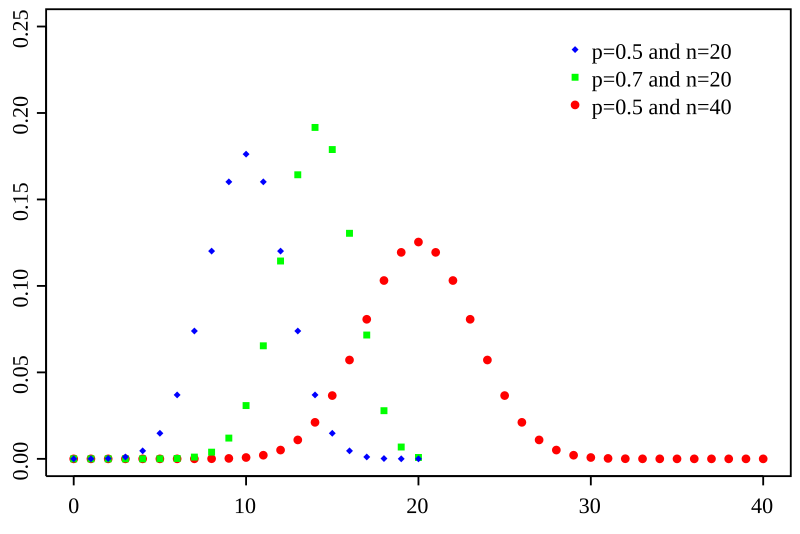
\includegraphics[
                width=\linewidth,
                height=5cm,
                keepaspectratio,
            ]{images/distributions/Binomial_distribution_pmf.svg.png}
            \caption{Binomial Distribution: PDF \cite{wiki/Binomial_distribution}}
        \end{figure}
    \end{minipage}
    \hfill
    \begin{minipage}{0.45\linewidth}
        \begin{figure}[H]
            \centering
            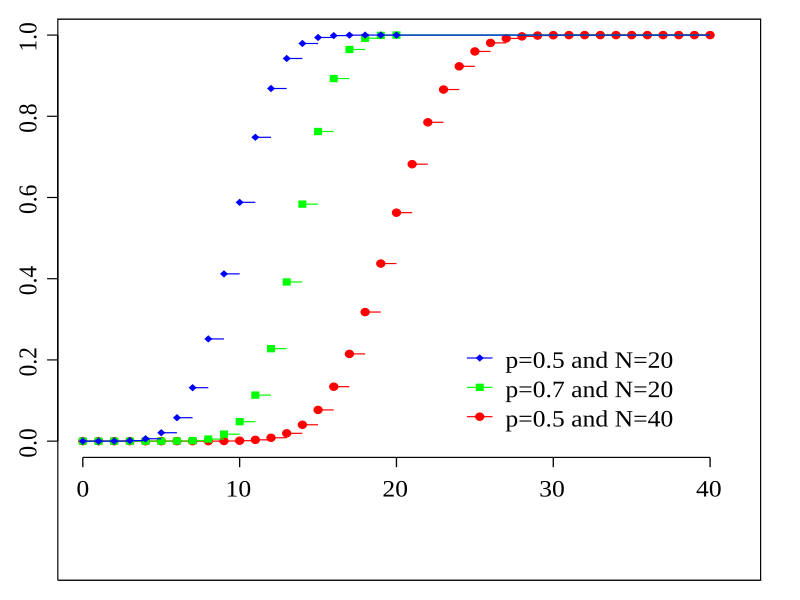
\includegraphics[
                width=\linewidth,
                height=5cm,
                keepaspectratio,
            ]{images/distributions/Binomial_distribution_cdf.svg.png}
            \caption{Binomial Distribution: CDF \cite{wiki/Binomial_distribution}}
        \end{figure}
    \end{minipage}
    \hfill
\end{table}





\begin{enumerate}
    \item A \textbf{disadvantage} of a random variable with a binomial distribution function is that it is bounded by the number of trials $n$.
    \hfill \cite{statistics/book/Statistics-for-Data-Scientists/Maurits-Kaptein}
\end{enumerate}





\subsection{PMF}

\begin{enumerate}
    \item binomial random variable $S_n$ is the sum of $n$ independent Bernoulli variables
    \hfill \cite{statistics/book/Statistics-for-Data-Scientists/Maurits-Kaptein}

    \item The random variable $S_n$ is then given by $S_n = X_1 + X_2 + \cdots + X _n$ , with $X_ k$ the binary random variable for turn $k$
    \hfill \cite{statistics/book/Statistics-for-Data-Scientists/Maurits-Kaptein}

    \item The PMF of the binomial is given by:
    \hfill \cite{statistics/book/Statistics-for-Data-Scientists/Maurits-Kaptein}
    \\
    $
        P(S_n = s)
        = f_{n,p}(s)
        = \displaystyle\binom{n}{s} p^s (1-p)^{n-s}
    $
    \hfill
    $
        \displaystyle\binom{n}{s} = \dfrac{n!}{s!(n-s)!}
    $
    \hfill \cite{statistics/book/Statistics-for-Data-Scientists/Maurits-Kaptein}
\end{enumerate}






\subsection{Summary}

\begin{enumerate}
    \item \textbf{Notation}:
    $
         {\displaystyle \mathcal{B}(n,p)}
    $
    \hfill \cite{wiki/Binomial_distribution}

    \item \textbf{Parameters}:
    \begin{enumerate}
        \item ${\displaystyle n\in \{0,1,2,\ldots \}}$ – number of trials
        \hfill \cite{wiki/Binomial_distribution}

        \item ${\displaystyle p\in [0,1]}$ – success probability for each trial
        \hfill \cite{wiki/Binomial_distribution}

        \item ${\displaystyle q=1-p}$ - failure probability for each trial
        \hfill \cite{wiki/Binomial_distribution}
    \end{enumerate}
    \hfill \cite{wiki/Binomial_distribution}

    \item \textbf{Support}:
     ${\displaystyle k\in \{0,1,\ldots ,n\}}$ – number of successes
    \hfill \cite{wiki/Binomial_distribution}

    \item \textbf{PMF}:
    $
         {\displaystyle {\binom {n}{k}}p^{k}q^{n-k}}
    $
    \hfill \cite{wiki/Binomial_distribution}

    \item \textbf{CDF}:
     ${\displaystyle I_{q}(n-\lfloor k\rfloor ,1+\lfloor k\rfloor )}$ (the regularized incomplete beta function)
    \hfill \cite{wiki/Binomial_distribution}

    \item \textbf{Mean}:
    $
         {\displaystyle np}
    $
    \hfill \cite{wiki/Binomial_distribution}

    \item \textbf{Median}:
    ${\displaystyle \lfloor np\rfloor }$ or ${\displaystyle \lceil np\rceil }$
    \hfill \cite{wiki/Binomial_distribution}

    \item \textbf{Mode}:
     ${\displaystyle \lfloor (n+1)p\rfloor }$ or ${\displaystyle \lceil (n+1)p\rceil -1}$
    \hfill \cite{wiki/Binomial_distribution}

    \item \textbf{Variance}:
    $
         {\displaystyle npq=np(1-p)}
    $
    \hfill \cite{wiki/Binomial_distribution}

    % \item \textbf{Median absolute deviation (MAD)}:
    % $

    % $
    % \hfill \cite{wiki/Binomial_distribution}

    \item \textbf{Skewness}:
    $
         {\displaystyle {\dfrac {q-p}{\sqrt {npq}}}}
    $
    \hfill \cite{wiki/Binomial_distribution}

    \item \textbf{Excess kurtosis}:
    $
         {\displaystyle {\dfrac {1-6pq}{npq}}}
    $
    \hfill \cite{wiki/Binomial_distribution}

    \item \textbf{Entropy}:
     ${\displaystyle {\dfrac {1}{2}}\log _{2}(2\pi enpq)+O\left({\dfrac {1}{n}}\right)}$ in shannons. For nats, use the natural log in the log.
    \hfill \cite{wiki/Binomial_distribution}

    \item \textbf{Moment-generating function (MGF)}:
    $
         {\displaystyle (q+pe^{t})^{n}}
    $
    \hfill \cite{wiki/Binomial_distribution}

    \item \textbf{Characteristic function (CF)}:
    $
         {\displaystyle (q+pe^{it})^{n}}
    $
    \hfill \cite{wiki/Binomial_distribution}

    \item \textbf{Probability-generating function (PGF)}:
    $
         {\displaystyle G(z)=[q+pz]^{n}}
    $
    \hfill \cite{wiki/Binomial_distribution}

    \item \textbf{Fisher information}:
    ${\displaystyle g_{n}(p)={\dfrac {n}{pq}}}$ (for fixed n ${\displaystyle n}$)
    \hfill \cite{wiki/Binomial_distribution}
\end{enumerate}






\section{Negative binomial distribution ($ {\displaystyle  {NB} (r,\,p)}$)}


\subsection{PMF}

\begin{enumerate}
    \item The negative binomial PMF is often considered a Poisson PMF with an extra amount of variation
    \hfill \cite{statistics/book/Statistics-for-Data-Scientists/Maurits-Kaptein}

    \item \textbf{Parameters}:
    \begin{enumerate}
        \item $\lambda$: mean, the same as for the Poisson random variable
        \hfill \cite{statistics/book/Statistics-for-Data-Scientists/Maurits-Kaptein}

        \item $\delta$: overdispersion parameter, indicating the extra amount of variation on top of the Poisson variation.
        \hfill \cite{statistics/book/Statistics-for-Data-Scientists/Maurits-Kaptein}
    \end{enumerate}

    \item A negative binomial random variable $X$ has its outcomes in the set $\dCurlyBrac{0, 1, 2, 3, ....}$, like the Poisson random variable.
    The PMF is defined by:
    \hfill \cite{statistics/book/Statistics-for-Data-Scientists/Maurits-Kaptein}
    \\
    $
        P(X=x)
        = f_{\lambda,\ \delta}(k)
        = \dfrac{\Gamma(k + \delta^{-1})}{\Gamma(k + 1)\ \Gamma(\delta^{-1})}
        \dfrac{(\delta\lambda)^k}{(1+\delta\lambda)^{k+\delta^{-1}}}
    $
    \hfill \cite{statistics/book/Statistics-for-Data-Scientists/Maurits-Kaptein}


    \item $\mu = \mathbb{E}[X] = \lambda$
    \hfill \cite{statistics/book/Statistics-for-Data-Scientists/Maurits-Kaptein}

    \item $\sigma^2 = \mathbb{E}[(X - \lambda)^2] = \lambda + \delta\lambda^2$
    \hfill \cite{statistics/book/Statistics-for-Data-Scientists/Maurits-Kaptein}

    \item In case the parameter $\delta$ converges to zero, the variance converges to the variance of a Poisson random variable.
    This is the reason that the parameter $\delta$ is called the overdispersion.
\end{enumerate}




\subsection{Summary}

\begin{enumerate}
    \item \textbf{Notation}:
    $
         {\displaystyle \mathrm {NB} (r,\,p)}
    $
    \hfill \cite{wiki/Negative_binomial_distribution}

    \item \textbf{Parameters}:
    $r > 0$ — number of successes until the experiment is stopped (integer, but the definition can also be extended to reals) $p \in [0, 1]$ — success probability in each experiment (real)
    \hfill \cite{wiki/Negative_binomial_distribution}

    \item \textbf{Support}:
     $k \in \dCurlyBrac{0, 1, 2, 3, \cdots}$ — number of failures
    \hfill \cite{wiki/Negative_binomial_distribution}

    \item \textbf{PMF}:
    ${\displaystyle k\mapsto {k+r-1 \choose k}\cdot (1-p)^{k}p^{r}}$
    involving a binomial coefficient
    \hfill \cite{wiki/Negative_binomial_distribution}

    \item \textbf{CDF}:
    ${\displaystyle k\mapsto I_{p}(r,\,k+1)}$
    the regularized incomplete beta function
    \hfill \cite{wiki/Negative_binomial_distribution}

    \item \textbf{Mean}:
    $
         {\displaystyle {\dfrac {r(1-p)}{p}}}
    $
    \hfill \cite{wiki/Negative_binomial_distribution}

    % \item \textbf{Median}:
    % $
    % $
    % \hfill \cite{wiki/Negative_binomial_distribution}

    \item \textbf{Mode}:
    $
         {\displaystyle {\begin{cases}\left\lfloor {\dfrac {(r-1)(1-p)}{p}}\right\rfloor &{\text{if }}r>1\\0&{\text{if }}r\leq 1\end{cases}}}
    $
    \hfill \cite{wiki/Negative_binomial_distribution}

    \item \textbf{Variance}:
    $
         {\displaystyle {\dfrac {r(1-p)}{p^{2}}}}
    $
    \hfill \cite{wiki/Negative_binomial_distribution}

    % \item \textbf{Median absolute deviation (MAD)}:
    % $
    % $
    % \hfill \cite{wiki/Negative_binomial_distribution}

    \item \textbf{Skewness}:
    $
         {\displaystyle {\dfrac {2-p}{\sqrt {(1-p)r}}}}
    $
    \hfill \cite{wiki/Negative_binomial_distribution}

    \item \textbf{Excess kurtosis}:
    $
         {\displaystyle {\dfrac {6}{r}}+{\dfrac {p^{2}}{(1-p)r}}}
    $
    \hfill \cite{wiki/Negative_binomial_distribution}

    % \item \textbf{Entropy}:
    % \hfill \cite{wiki/Negative_binomial_distribution}

    \item \textbf{Moment-generating function (MGF)}:
    $
         {\displaystyle {\biggl (}{\dfrac {p}{1-(1-p)e^{t}}}{\biggr )}^{\!r}{\text{ for }}t<-\log(1-p)}
    $
    \hfill \cite{wiki/Negative_binomial_distribution}

    \item \textbf{Characteristic function (CF)}:
    $
         {\displaystyle {\biggl (}{\dfrac {p}{1-(1-p)e^{i\,t}}}{\biggr )}^{\!r}{\text{ with }}t\in \mathbb {R} }
    $
    \hfill \cite{wiki/Negative_binomial_distribution}

    \item \textbf{Probability-generating function (PGF)}:
    $
         {\displaystyle {\biggl (}{\dfrac {p}{1-(1-p)z}}{\biggr )}^{\!r}{\text{ for }}|z|<{\dfrac {1}{p}}}
    $
    \hfill \cite{wiki/Negative_binomial_distribution}

    \item \textbf{Fisher information}:
    $
         {\displaystyle {\dfrac {r}{p^{2}(1-p)}}}
    $
    \hfill \cite{wiki/Negative_binomial_distribution}

    \item \textbf{Method of moments}:
    $ {\displaystyle r={\dfrac {\mbbE[X]^{2}}{\mbbV[X]-\mbbE[X]}}}$
    \hspace{1cm}
    $ {\displaystyle p={\dfrac {\mbbE[X]}{\mbbV[X]}}}$
    \hfill \cite{wiki/Negative_binomial_distribution}
\end{enumerate}









\section{Poisson distribution}

\begin{table}[H]
    \hfill
    \begin{minipage}{0.45\linewidth}
        \begin{figure}[H]
            \centering
            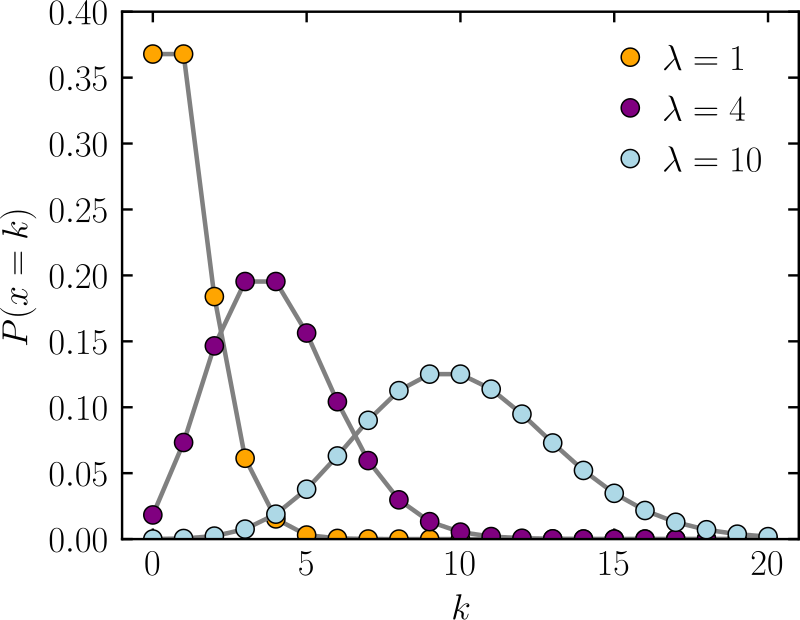
\includegraphics[
                width=\linewidth,
                height=5cm,
                keepaspectratio,
            ]{images/distributions/Poisson_pmf.svg.png}
            \caption{Poisson distribution: PDF \cite{wiki/Poisson_distribution}}
        \end{figure}
    \end{minipage}
    \hfill
    \begin{minipage}{0.45\linewidth}
        \begin{figure}[H]
            \centering
            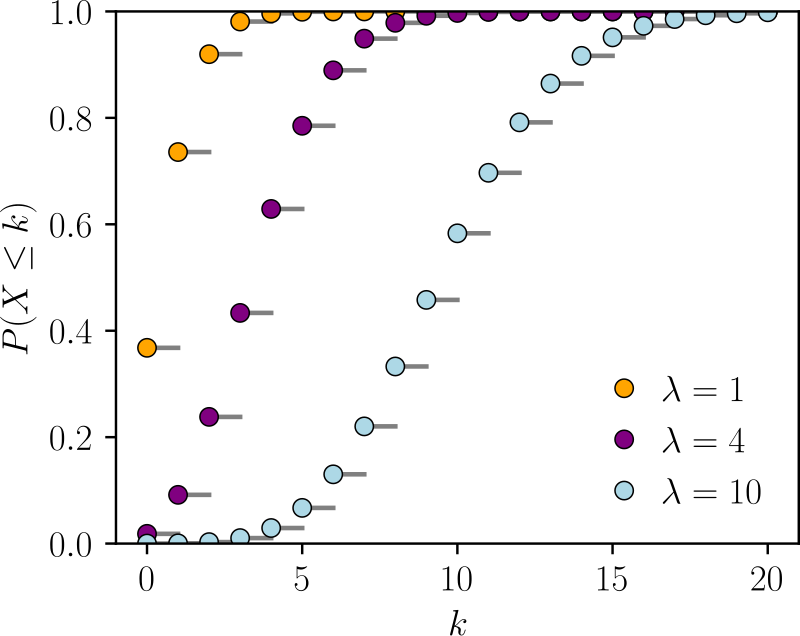
\includegraphics[
                width=\linewidth,
                height=5cm,
                keepaspectratio,
            ]{images/distributions/Poisson_cdf.svg.png}
            \caption{Poisson distribution: CDF \cite{wiki/Poisson_distribution}}
        \end{figure}
    \end{minipage}
    \hfill
\end{table}







\subsection{Summary}

\begin{enumerate}
    \item \textbf{Notation}:
    $
         {\displaystyle \operatorname {Pois} (\lambda )}
    $
    \hfill \cite{wiki/Poisson_distribution}

    \item \textbf{Parameters}:
    ${\displaystyle \lambda \in (0,\infty )}$ (rate)
    \hfill \cite{wiki/Poisson_distribution}

    \item \textbf{Support}:
    ${\displaystyle k\in \mathbb {N} _{0}}$ (Natural numbers starting from $0$)
    \hfill \cite{wiki/Poisson_distribution}

    \item \textbf{PMF}:
    $
         {\displaystyle {\dfrac {\lambda ^{k}e^{-\lambda }}{k!}}}
    $
    \hfill \cite{wiki/Poisson_distribution}

    \item \textbf{CDF}:
    ${\displaystyle {\dfrac {\Gamma (\lfloor k+1\rfloor ,\lambda )}{\lfloor k\rfloor !}},}$ or
    ${\displaystyle e^{-\lambda }\sum _{j=0}^{\lfloor k\rfloor }{\dfrac {\lambda ^{j}}{j!}},}$ or
    ${\displaystyle Q(\lfloor k+1\rfloor ,\lambda )}$
    (for ${\displaystyle k\geq 0,}$ where ${\displaystyle \Gamma (x,y)}$ is the upper incomplete gamma function, ${\displaystyle \lfloor k\rfloor }$ is the floor function, and ${\displaystyle Q}$ is the regularized gamma function)
    \hfill \cite{wiki/Poisson_distribution}

    \item \textbf{Mean}:
    $
         {\displaystyle \lambda }
    $
    \hfill \cite{wiki/Poisson_distribution}

    \item \textbf{Median}:
    $
         {\displaystyle \approx \left\lfloor \lambda +{\dfrac {1}{3}}-{\dfrac {1}{50\lambda }}\right\rfloor }
    $
    \hfill \cite{wiki/Poisson_distribution}

    \item \textbf{Mode}:
    $
         {\displaystyle \left\lceil \lambda \right\rceil -1,\left\lfloor \lambda \right\rfloor }
    $
    \hfill \cite{wiki/Poisson_distribution}

    \item \textbf{Variance}:
    $
         {\displaystyle \lambda }
    $
    \hfill \cite{wiki/Poisson_distribution}

    % \item \textbf{Median absolute deviation (MAD)}:
    % $
    % $
    % \hfill \cite{wiki/Poisson_distribution}

    \item \textbf{Skewness}:
    $
         {\displaystyle {\dfrac {1}{\sqrt {\lambda }}}}
    $
    \hfill \cite{wiki/Poisson_distribution}

    \item \textbf{Excess kurtosis}:
    $
         {\displaystyle {\dfrac {1}{\lambda }}}
    $
    \hfill \cite{wiki/Poisson_distribution}

    \item \textbf{Entropy}:
    ${\displaystyle \lambda {\Bigl [}1-\log(\lambda ){\Bigr ]}+e^{-\lambda }\sum _{k=0}^{\infty }{\dfrac {\lambda ^{k}\log(k!)}{k!}}}$
    or for large ${\displaystyle \lambda }$
    ${\displaystyle {\begin{aligned}\approx {\dfrac {1}{2}}\log \left(2\pi e\lambda \right)-{\dfrac {1}{12\lambda }}-{\dfrac {1}{24\lambda ^{2}}}\\-{\dfrac {19}{360\lambda ^{3}}}+{\mathcal {O}}\left({\dfrac {1}{\lambda ^{4}}}\right)\end{aligned}}}$
    \hfill \cite{wiki/Poisson_distribution}

    \item \textbf{Moment-generating function (MGF)}:
    $
         {\displaystyle \exp \left[\lambda \left(e^{t}-1\right)\right]}
    $
    \hfill \cite{wiki/Poisson_distribution}

    \item \textbf{Characteristic function (CF)}:
    $
         {\displaystyle \exp \left[\lambda \left(e^{it}-1\right)\right]}
    $
    \hfill \cite{wiki/Poisson_distribution}

    \item \textbf{Probability-generating function (PGF)}:
    $
         {\displaystyle \exp \left[\lambda \left(z-1\right)\right]}
    $
    \hfill \cite{wiki/Poisson_distribution}

    \item \textbf{Fisher information}:
    $
         {\displaystyle {\dfrac {1}{\lambda }}}
    $
    \hfill \cite{wiki/Poisson_distribution}
\end{enumerate}




\subsection{Standard Error of MLE}

\begin{enumerate}
    \item let $X_1 , X_2, \cdots , X_n$ be i.i.d. Poisson $\mathcal{P}(\lambda)$ distributed. 
    \hfill \cite{statistics/book/Statistics-for-Data-Scientists/Maurits-Kaptein}

    \item population mean $\mu ( f ) = \lambda $ and the population variance $\sigma 2( f ) = \lambda $. 
    \hfill \cite{statistics/book/Statistics-for-Data-Scientists/Maurits-Kaptein}

    \item The maximum likelihood estimator for $\theta = \lambda$ , which is also the moment estimator, is given by the sample average $\hat{\lambda} = \bar{X}$. 
    \hfill \cite{statistics/book/Statistics-for-Data-Scientists/Maurits-Kaptein}

    \item  the log likelihood is $\ell _\theta = \dsum^n _{i=1}[X_i \log(\lambda ) - \log(X_i !) - \lambda ]$. 
    \hfill \cite{statistics/book/Statistics-for-Data-Scientists/Maurits-Kaptein}

    \item Equating the derivative with respect to $\lambda $ to zero results into $\dsum \dParenBrac{\dfrac{X_i}{\lambda} - 1} = 0$. 
    Solving this for $\lambda $ gives $\hat{\lambda} = \bar{X}$.
    \hfill \cite{statistics/book/Statistics-for-Data-Scientists/Maurits-Kaptein}

    \item As the distribution of $\dfrac{\sqrt{n}( \bar{X} - \mu ( f ))}{\sigma ( f )}$ converges to a standard normal distribution, $\sqrt{n}( \bar{X} - \lambda )$ converges to $\mathcal{N} (0, \lambda )$
    \hfill \cite{statistics/book/Statistics-for-Data-Scientists/Maurits-Kaptein}

    \item he Fisher information for the Poisson distribution is given by $I (\lambda ) = \mbbE\dSquareBrac{\dParenBrac{\dfrac{X}{\lambda} - 1}2}=  \mbbE\dSquareBrac{\dParenBrac{\dfrac{X - \lambda}{\lambda}}^2} = \dfrac{1}{\lambda} $ .
    \hfill \cite{statistics/book/Statistics-for-Data-Scientists/Maurits-Kaptein}

    \item Thus, the asymptotic variance of the MLE is given by $I ^{-1}(\lambda ) = \lambda $ and the standard error of $\bar{X}$ is equal to $\sqrt{\dfrac{\lambda}{n}}$.
    \hfill \cite{statistics/book/Statistics-for-Data-Scientists/Maurits-Kaptein}
\end{enumerate}
























\chapter{Continuous Distributions}


\section{Normal Distribution/ Gaussian Distribution (${N}(\mu, \sigma^2)$)}


\begin{table}[H]
    \hfill
    \begin{minipage}{0.45\linewidth}
        \begin{figure}[H]
            \centering
            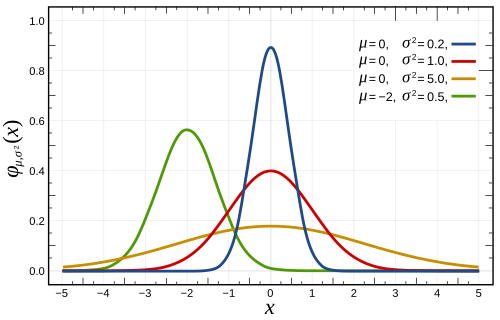
\includegraphics[
                width=\linewidth,
                height=5cm,
                keepaspectratio,
            ]{images/distributions/Normal_Distribution_PDF.svg.png}
            \caption{Normal Distribution: PDF \cite{wiki/Normal_distribution}}
        \end{figure}
    \end{minipage}
    \hfill
    \begin{minipage}{0.45\linewidth}
        \begin{figure}[H]
            \centering
            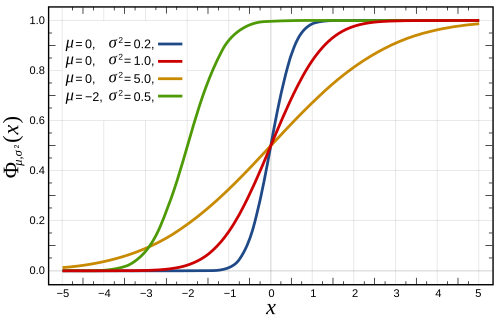
\includegraphics[
                width=\linewidth,
                height=5cm,
                keepaspectratio,
            ]{images/distributions/Normal_Distribution_CDF.svg.png}
            \caption{Normal Distribution: CDF \cite{wiki/Normal_distribution}}
        \end{figure}
    \end{minipage}
    \hfill
\end{table}

\begin{enumerate}
    \item Denoted by: $\mathcal{N}(\mu, \sigma^2)$
\end{enumerate}


\subsection{PDF ($f_{\mu, \sigma}(x)$ or $f(x|\mu, \sigma)$)}

\begin{enumerate}
    \item[]  $
        f_{\mu, \sigma}(x)
        = \dfrac{1}{\sigma\sqrt{2\pi}} \exp\dParenBrac{-\dfrac{(x-\mu)^2}{2\sigma^2}}
    $ 
    \hfill \cite{statistics/book/Statistics-for-Data-Scientists/Maurits-Kaptein}
    \begin{enumerate}
        \item[] $\mu \in \mbbR$: indicates the mean value of the population of the variable of interest
        \hfill \cite{statistics/book/Statistics-for-Data-Scientists/Maurits-Kaptein}

        \item[] $\sigma$: indicates the standard deviation ($\sigma^2 > 0$)
        \hfill \cite{statistics/book/Statistics-for-Data-Scientists/Maurits-Kaptein}
    \end{enumerate}

    \item[] $f_{\mu, \sigma}(x) = \dfrac{1}{\sigma}\phi\dParenBrac{\dfrac{x-\mu}{\sigma}}$
    \hfill \cite{statistics/book/Statistics-for-Data-Scientists/Maurits-Kaptein}

    \item it can be used to approximate other PDFs when the sample size or the size of the data is getting large.
    \hfill \cite{statistics/book/Statistics-for-Data-Scientists/Maurits-Kaptein}

    \item This has the advantage that important features of the normal density function can be transferred to other densities when the approximation is quite close. 
    \hfill \cite{statistics/book/Statistics-for-Data-Scientists/Maurits-Kaptein}

    \item The shape of the normal PDF is equal to the famous “bell-shape” curve 
    \hfill \cite{statistics/book/Statistics-for-Data-Scientists/Maurits-Kaptein}

    \item areas under the curve:
    \begin{enumerate}
        \item $99.73\%$ of all the population values fall within the interval $[\mu - 3\sigma, \mu + 3\sigma]$
        \hfill \cite{statistics/book/Statistics-for-Data-Scientists/Maurits-Kaptein}
    
        \item $95.45\%$ of all the population values fall within the interval $[\mu - 2\sigma, \mu + 2\sigma]$ or 
        \hfill \cite{statistics/book/Statistics-for-Data-Scientists/Maurits-Kaptein}
        \\
        $
            \dint_{\mu - 2\sigma}^{\mu + 2\sigma}
            \phi\dParenBrac{\dfrac{x-\mu}{\sigma}} dx
            = 
            \dint_{-2}^{2}
            \phi(x) dx
            =
            0.9545
        $
        \hfill \cite{statistics/book/Statistics-for-Data-Scientists/Maurits-Kaptein}

        \item $95\%$ of the values fall within $[\mu - 1.96\sigma, \mu + 1.96\sigma]$
        \hfill \cite{statistics/book/Statistics-for-Data-Scientists/Maurits-Kaptein}
    \end{enumerate}

    \item  describes both positive and negative values
    \hfill \cite{statistics/book/Statistics-for-Data-Scientists/Maurits-Kaptein}

    \item a random measurement error that could be described by a normal PDF is more likely to be closer to zero than to be further away from zero (due to the bell shape of the density). 
    \hfill \cite{statistics/book/Statistics-for-Data-Scientists/Maurits-Kaptein}
\end{enumerate}




\subsection{Summary}

\begin{enumerate}

    \item 
    \textbf{Notation}:
    $
        {\displaystyle {\mathcal {N}}(\mu ,\sigma ^{2})}
    $
    \hfill \cite{wiki/Normal_distribution} 

    \item 
    \textbf{Parameters}:
    \begin{enumerate}
        \item ${\displaystyle \mu \in \mathbb {R} }$ = mean (location)
        \hfill \cite{wiki/Normal_distribution}

        \item ${\displaystyle \sigma ^{2}\in \mathbb {R} _{>0}}$ = variance (squared scale)
        \hfill \cite{wiki/Normal_distribution}
    \end{enumerate}

    \item 
    \textbf{Support/ Rand Var}: 
    $x \in \mbbR$ 
    \hfill \cite{wiki/Normal_distribution}

    \item 
    \textbf{PDF}: 
    $ {\displaystyle {\dfrac {1}{\sqrt {2\pi \sigma ^{2}}}}e^{-{\dfrac {(x-\mu )^{2}}{2\sigma ^{2}}}}} $ 
    \hfill\cite{wiki/Normal_distribution}

    \item 
    \textbf{CDF}: 
    $ {\displaystyle \Phi \left({\dfrac {x-\mu }{\sigma }}\right)={\dfrac {1}{2}}\left[1+\operatorname {erf} \left({\dfrac {x-\mu }{\sigma {\sqrt {2}}}}\right)\right]} $ 
    \hfill\cite{wiki/Normal_distribution}

    \item 
    \textbf{Quantile}:
    $ {\displaystyle \mu +\sigma {\sqrt {2}}\operatorname {erf} ^{-1}(2p-1)} $ 
    \hfill\cite{wiki/Normal_distribution}

    \item 
    \textbf{Mean}:
    $ {\displaystyle \mu } $ 
    \hfill\cite{wiki/Normal_distribution}

    \item 
    \textbf{Median}:
    $ {\displaystyle \mu } $ 
    \hfill\cite{wiki/Normal_distribution}

    \item 
    \textbf{Mode}:
    $ {\displaystyle \mu } $ 
    \hfill\cite{wiki/Normal_distribution}

    \item 
    \textbf{Variance}:
    $ {\displaystyle \sigma ^{2}} $
    \hfill\cite{wiki/Normal_distribution}

    \item 
    \textbf{Median absolute deviation (MAD)}:
    $ {\displaystyle \sigma {\sqrt {2}}\,\operatorname {erf} ^{-1}(1/2)} $
    \hfill\cite{wiki/Normal_distribution}

    \item 
    \textbf{Average absolute deviation (AAD)}:
    $ {\textstyle \sigma {\sqrt {2/\pi }}} $
    \hfill\cite{wiki/Normal_distribution}

    \item 
    \textbf{Skewness}: $0$
    \hfill\cite{wiki/Normal_distribution}

    \item 
    \textbf{Excess kurtosis}: $0$
    \hfill\cite{wiki/Normal_distribution}

    \item 
    \textbf{Entropy}: $ {\textstyle {\tfrac {1}{2}}\log(2\pi e\sigma ^{2})} $
    \hfill\cite{wiki/Normal_distribution}

    \item 
    \textbf{Moment-generating function (MGF)}: $ {\displaystyle \exp(\mu t+\sigma ^{2}t^{2}/2)} $ 
    \hfill\cite{wiki/Normal_distribution}

    \item 
    \textbf{Characteristic function (CF)}: $ {\displaystyle \exp(i\mu t-\sigma ^{2}t^{2}/2)} $ 
    \hfill\cite{wiki/Normal_distribution}

    \item 
    \textbf{Fisher information}:
    \begin{enumerate}
        \item ${\displaystyle {\mathcal {I}}(\mu ,\sigma )={\begin{pmatrix}1/\sigma ^{2}&0\\0&2/\sigma ^{2}\end{pmatrix}}}$

        \item ${\displaystyle {\mathcal {I}}(\mu ,\sigma ^{2})={\begin{pmatrix}1/\sigma ^{2}&0\\0&1/(2\sigma ^{4})\end{pmatrix}}}$
    \end{enumerate}
    \hfill\cite{wiki/Normal_distribution}
    
    \item 
    \textbf{Kullback–Leibler divergence}:
    ${\displaystyle D_{KL} = {1 \over 2}\left\{\left({\dfrac {\sigma _{0}}{\sigma _{1}}}\right)^{2}+{\dfrac {(\mu _{1}-\mu _{0})^{2}}{\sigma _{1}^{2}}}-1+\ln {\sigma _{1}^{2} \over \sigma _{0}^{2}}\right\}}$
    \hfill\cite{wiki/Normal_distribution}

    \item 
    \textbf{Expected shortfall}:
    ${\displaystyle \mu +\sigma {\dfrac {{\dfrac {1}{\sqrt {2\pi }}}e^{\dfrac {-\left(q_{p}\left({\dfrac {X-\mu }{\sigma }}\right)\right)^{2}}{2}}}{1-p}}}$
    \hfill\cite{wiki/Normal_distribution}

\end{enumerate}


\section{Standard Normal Distribution (${N}(0, 1)$)}

\begin{enumerate}
    \item When we choose $\mu = 0$ and $\sigma = 1$ in a Normal Distribution, its called Standard Normal Distribution.
    \hfill \cite{statistics/book/Statistics-for-Data-Scientists/Maurits-Kaptein}


\end{enumerate}


\subsection{PDF ($f(x)$ or $f(x)$ or $\phi(x)$)}

\begin{enumerate}
    \item[] $\phi(x) = \dfrac{\exp(-x^2/2)}{\sqrt{2\pi}}$
    \hfill \text{\cite{statistics/book/Statistics-for-Data-Scientists/Maurits-Kaptein}}


\end{enumerate}



\subsection{Bivariate Standard Normal Distribution}

\begin{enumerate}
    \item Consider a bivariate standard Gaussian random variable $X$ and performed a linear transformation $\bm{Ax}$ on it. 
    \hfill \cite{mfml/book/mml/Deisenroth-Faisal-Ong}

    \item The outcome is a Gaussian random variable with mean zero and covariance $\bm{AA}^\top$.
    \hfill \cite{mfml/book/mml/Deisenroth-Faisal-Ong}

    \item Adding a constant vector will change the mean of the distribution, without affecting its variance, that is, the random variable $\bm{x} + \bm{\mu}$ is Gaussian with mean $\bm{\mu}$ and identity covariance.
    Hence, any linear/affine transformation of a Gaussian random variable is Gaussian distributed.
    \hfill \cite{mfml/book/mml/Deisenroth-Faisal-Ong}

\end{enumerate}















\section{Lognormal Distribution ($\text{Lognormal}(\mu ,\sigma ^{2})$)}

\begin{table}[H]
    \hfill
    \begin{minipage}{0.45\linewidth}
        \begin{figure}[H]
            \centering
            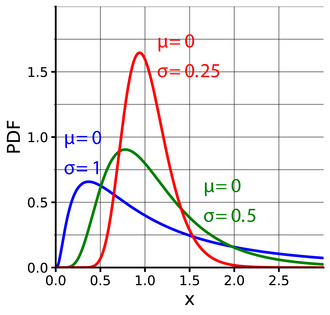
\includegraphics[
                width=\linewidth,
                height=5cm,
                keepaspectratio,
            ]{images/distributions/Log-normal-pdfs.png}
            \caption{Lognormal Distribution: PDF \cite{wiki/Log-normal_distribution}}
        \end{figure}
    \end{minipage}
    \hfill
    \begin{minipage}{0.45\linewidth}
        \begin{figure}[H]
            \centering
            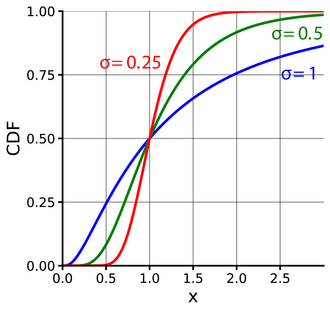
\includegraphics[
                width=\linewidth,
                height=5cm,
                keepaspectratio,
            ]{images/distributions/Log-normal-cdfs.png}
            \caption{Lognormal Distribution: CDF \cite{wiki/Log-normal_distribution}}
        \end{figure}
    \end{minipage}
    \hfill
\end{table}



\subsection{PDF}

\begin{enumerate}
    \item[] $
        f_{\mu, \sigma}(x) = \dfrac{1}{x\sigma \sqrt{2\pi}} \exp\dCurlyBrac{
            -\dfrac{(\log(x) - \mu)^2}{2\sigma^2}
        }
    $
    \hfill \cite{statistics/book/Statistics-for-Data-Scientists/Maurits-Kaptein}
    
    \item the lognormal PDF describes populations with positive values
    \hfill \cite{statistics/book/Statistics-for-Data-Scientists/Maurits-Kaptein}

    \item relative standard deviation  is constant for the lognormal PDF. 
    This means that larger values demonstrate larger variability, but the ratio with variability is constant whether we observe smaller or larger values. 
    \hfill \cite{statistics/book/Statistics-for-Data-Scientists/Maurits-Kaptein}

    \item the lognormal PDF is not symmetric like the normal PDF, which makes sense when values are limited from below, but not from above.
    \hfill \cite{statistics/book/Statistics-for-Data-Scientists/Maurits-Kaptein}

    \item  If the population values can be described by a lognormal PDF, the normal PDF would then describe the logarithmic transformation of the population values (using the natural logarithm).
    \hfill \cite{statistics/book/Statistics-for-Data-Scientists/Maurits-Kaptein}

    \item The parameters $\mu$ and $\sigma$ have a different meaning in the lognormal PDF than in the normal PDF. 
    They do represent the population mean and standard deviation, but only for the logarithmic transformed values of the population. 
    Their meaning in relation to the mean and standard deviation of the population values in the original scale is now more complicated. 
    \hfill \cite{statistics/book/Statistics-for-Data-Scientists/Maurits-Kaptein}
\end{enumerate}



\subsection{Summary}

\begin{enumerate}
    \item \textbf{Notation}: 
    ${\displaystyle \operatorname {Lognormal} \left(\mu ,\,\sigma ^{2}\right)}$
    \hfill \cite{wiki/Log-normal_distribution}

    \item \textbf{Parameters}:
    \begin{enumerate}
        \item ${\displaystyle \mu \in (-\infty ,+\infty )}$: logarithm of location
        \hfill \cite{wiki/Log-normal_distribution, statistics/book/Statistics-for-Data-Scientists/Maurits-Kaptein}

        \item ${\displaystyle \sigma >0}$: logarithm of scale
        \hfill \cite{wiki/Log-normal_distribution, statistics/book/Statistics-for-Data-Scientists/Maurits-Kaptein}
    \end{enumerate}

    \item \textbf{Support}: ${\displaystyle x\in (0,+\infty )}$
    \hfill \cite{wiki/Log-normal_distribution, statistics/book/Statistics-for-Data-Scientists/Maurits-Kaptein}

    \item \textbf{PDF}:
    ${\displaystyle {\dfrac {1}{x\sigma {\sqrt {2\pi }}}}\exp \left(-{\dfrac {\left(\ln x-\mu \right)^{2}}{2\sigma ^{2}}}\right)}$
    \hfill \cite{wiki/Log-normal_distribution, statistics/book/Statistics-for-Data-Scientists/Maurits-Kaptein}

    \item \textbf{CDF}:
    $
        {\displaystyle {{\dfrac {1}{2}}\left[1+\operatorname {erf} \left({\dfrac {\ln x-\mu }{\sigma {\sqrt {2}}}}\right)\right] 
        =\Phi {\left({\dfrac {\ln x-\mu }{\sigma }}\right)}}}
    $
    \hfill \cite{wiki/Log-normal_distribution}

    \item \textbf{Quantile}: 
    $
        {\displaystyle {\exp \left(\mu +{\sqrt {2\sigma ^{2}}}\operatorname {erf} ^{-1}(2p-1)\right)
        =\exp(\mu +\sigma \Phi ^{-1}(p))}}
    $
    \hfill \cite{wiki/Log-normal_distribution}

    \item \textbf{Mean}: ${\displaystyle \exp \left(\mu +{\dfrac {\sigma ^{2}}{2}}\right)}$
    \hfill \cite{wiki/Log-normal_distribution}

    \item \textbf{Median}: ${\displaystyle \exp(\mu )}$
    \hfill \cite{wiki/Log-normal_distribution}

    \item \textbf{Mode}: ${\displaystyle \exp \left(\mu -\sigma ^{2}\right)}$
    \hfill \cite{wiki/Log-normal_distribution}

    \item \textbf{Variance}: 
    ${\displaystyle \left[\exp(\sigma ^{2})-1\right]\exp \left(2\mu +\sigma ^{2}\right)}$
    \hfill \cite{wiki/Log-normal_distribution}

    \item \textbf{Skewness}:
    ${\displaystyle \left[\exp \left(\sigma ^{2}\right)+2\right]{\sqrt {\exp(\sigma ^{2})-1}}}$
    \hfill \cite{wiki/Log-normal_distribution}

    \item \textbf{Excess kurtosis}: 
    ${\displaystyle \exp \left(4\sigma ^{2}\right)+2\exp \left(3\sigma ^{2}\right)+3\exp \left(2\sigma ^{2}\right)-6}$
    \hfill \cite{wiki/Log-normal_distribution}

    \item \textbf{Entropy}: ${\displaystyle \log _{2}\left({\sqrt {2\pi e}}\,\sigma e^{\mu }\right)}$
    \hfill \cite{wiki/Log-normal_distribution}

    \item \textbf{Fisher information}: 
    ${\displaystyle {\dfrac {1}{\sigma ^{2}}}{\begin{pmatrix}1&0\\0&2\end{pmatrix}}}$
    \hfill \cite{wiki/Log-normal_distribution}

    \item \textbf{Method of moments}:
    \begin{enumerate}
        \item ${\displaystyle \mu =\ln \operatorname {E} [X]-{\dfrac {1}{2}}\ln \left({\dfrac {\operatorname {Var} [X]}{\operatorname {E} [X]^{2}}}+1\right),}$
        \hfill \cite{wiki/Log-normal_distribution}

        \item ${\displaystyle \sigma ={\sqrt {\ln \left({\dfrac {\operatorname {Var} [X]}{\operatorname {E} [X]^{2}}}+1\right)}}}$
        \hfill \cite{wiki/Log-normal_distribution}
    \end{enumerate}

    \item \textbf{Expected shortfall}:
    $
        {\displaystyle {{\dfrac {e^{\mu +{\dfrac {\sigma ^{2}}{2}}}}{2p}}\left[1+\text{erf} \left({\dfrac {\sigma }{\sqrt {2}}}+\operatorname {erf} ^{-1}(2p-1)\right)\right]
        ={\dfrac {e^{\mu +{\dfrac {\sigma ^{2}}{2}}}}{1-p}}\left[1-\Phi (\Phi ^{-1}(p)-\sigma )\right]}}
    $
    \hfill \cite{wiki/Log-normal_distribution}

    \item \textbf{Relative Standard Deviation}: $\sqrt{\exp\dCurlyBrac{\sigma^2} - 1}$
    \hfill \cite{statistics/book/Statistics-for-Data-Scientists/Maurits-Kaptein}
    \\
    (RSD = standard deviation divided by the mean)
    \hfill \cite{statistics/book/Statistics-for-Data-Scientists/Maurits-Kaptein}
\end{enumerate}







\section{(Continuous) Uniform Distribution ( $U(a, b)$ )}

\begin{table}[H]
    \hfill
    \begin{minipage}{0.45\linewidth}
        \begin{figure}[H]
            \centering
            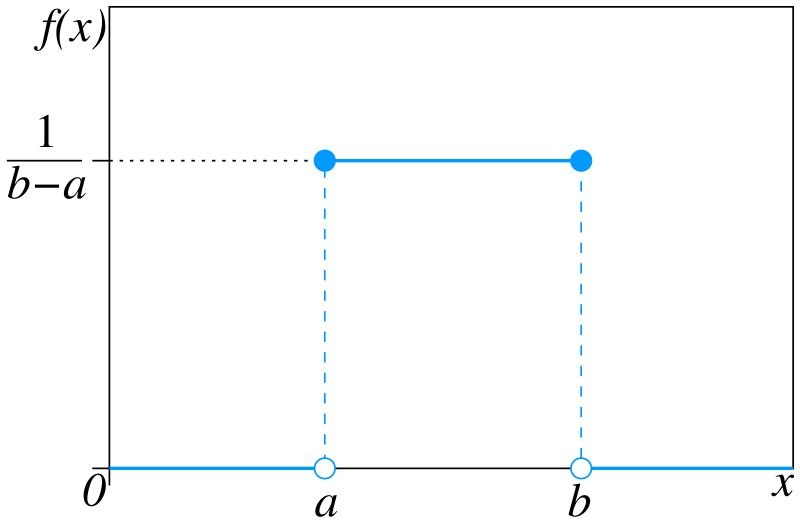
\includegraphics[
                width=\linewidth,
                height=5cm,
                keepaspectratio,
            ]{images/distributions/Uniform_Distribution_PDF_SVG.svg}
            \caption{Uniform Distribution: PDF \cite{wiki/Continuous_uniform_distribution}}
        \end{figure}
    \end{minipage}
    \hfill
    \begin{minipage}{0.45\linewidth}
        \begin{figure}[H]
            \centering
            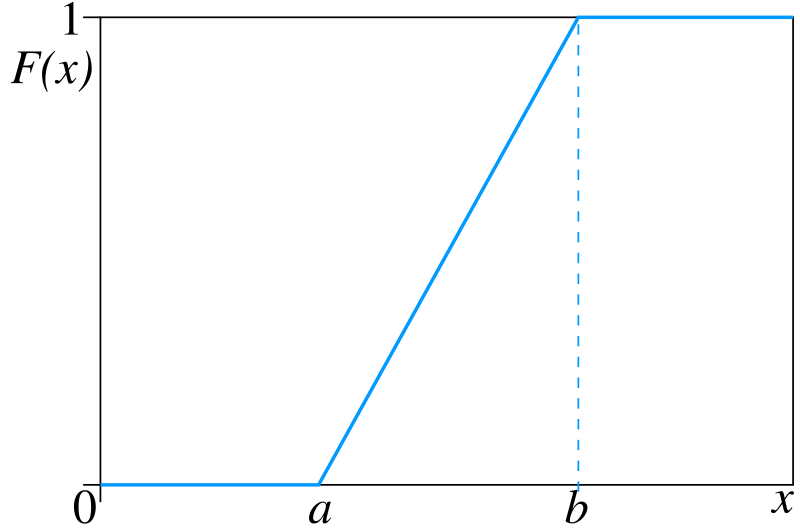
\includegraphics[
                width=\linewidth,
                height=5cm,
                keepaspectratio,
            ]{images/distributions/Uniform_Distribution_CDF_SVG.svg}
            \caption{Uniform Distribution: CDF \cite{wiki/Continuous_uniform_distribution}}
        \end{figure}
    \end{minipage}
    \hfill
\end{table}

\subsection{PDF}

\begin{enumerate}
    \item[] $f_{a,b}(x) = \dfrac {1}{b-a}, \hspace{1cm} x \in [a, b]$
    \hfill \cite{statistics/book/Statistics-for-Data-Scientists/Maurits-Kaptein}

    \item If the random measurement error would be described by a uniform PDF, being close to or far away form zero would be equally likely. 
    However, the uniform PDF has a finite domain, which means that the density is positive on an interval, say $[a, b]$, with $a < b$ and $a, b \in \mbbR$, but zero everywhere else.
    \hfill \cite{statistics/book/Statistics-for-Data-Scientists/Maurits-Kaptein}
\end{enumerate}



\subsection{Summary}

\begin{enumerate}
    \item \textbf{Notation}: 
    ${\displaystyle {\mathcal {U}}_{[a,b]}}$
    \hfill \cite{wiki/Continuous_uniform_distribution}

    \item \textbf{Parameters}:
    ${\displaystyle -\infty <a<b<\infty }$
    \hfill \cite{wiki/Continuous_uniform_distribution}

    \item \textbf{Support}: $[a, b]$
    \hfill \cite{wiki/Continuous_uniform_distribution}

    \item \textbf{PDF}:
    $ 
        {\displaystyle {\begin{cases}{\dfrac {1}{b-a}}&{\text{for }}x\in [a,b]\\0&{\text{otherwise}}\end{cases}}}
    $
    \hfill \cite{wiki/Continuous_uniform_distribution, statistics/book/Statistics-for-Data-Scientists/Maurits-Kaptein}

    \item \textbf{CDF}:
    $
        {\displaystyle {\begin{cases}0&{\text{for }}x<a\\{\dfrac {x-a}{b-a}}&{\text{for }}x\in [a,b]\\1&{\text{for }}x>b\end{cases}}}
    $
    \hfill \cite{wiki/Continuous_uniform_distribution}

    \item \textbf{Mean}: 
    $ 
        {\displaystyle {\dfrac {1}{2}}(a+b)}
    $
    \hfill \cite{wiki/Continuous_uniform_distribution}

    \item \textbf{Median}: 
    $ 
        {\displaystyle {\dfrac {1}{2}}(a+b)}
    $
    \hfill \cite{wiki/Continuous_uniform_distribution}

    \item \textbf{Mode}: 
    any value in $ {\displaystyle (a,b)} $
    \hfill \cite{wiki/Continuous_uniform_distribution}

    \item \textbf{Variance}: 
    $ 
        {\displaystyle {\dfrac {1}{12}}(b-a)^{2}}
    $
    \hfill \cite{wiki/Continuous_uniform_distribution}

    \item \textbf{Median absolute deviation (MAD)}: 
    $
        {\displaystyle {\dfrac {1}{4}}(b-a)}
    $
    \hfill \cite{wiki/Continuous_uniform_distribution}

    \item \textbf{Skewness}:
    $0$
    \hfill \cite{wiki/Continuous_uniform_distribution}

    \item \textbf{Excess kurtosis}: 
    $ -\dfrac{6}{5}$
    \hfill \cite{wiki/Continuous_uniform_distribution}

    \item \textbf{Entropy}: $ {\displaystyle \log(b-a)} $
    \hfill \cite{wiki/Continuous_uniform_distribution}

    \item \textbf{Moment-generating function (MGF)}: 
    $
        {\displaystyle {\begin{cases}{\dfrac {\mathrm {e} ^{tb}-\mathrm {e} ^{ta}}{t(b-a)}}&{\text{for }}t\neq 0\\1&{\text{for }}t=0\end{cases}}}
    $
    \hfill \cite{wiki/Continuous_uniform_distribution}
    
    \item \textbf{Characteristic function (CF)}:
    $
        {\displaystyle {\begin{cases}{\dfrac {\mathrm {e} ^{\mathrm {i} tb}-\mathrm {e} ^{\mathrm {i} ta}}{\mathrm {i} t(b-a)}}&{\text{for }}t\neq 0\\1&{\text{for }}t=0\end{cases}}}
    $
    \hfill \cite{wiki/Continuous_uniform_distribution}

\end{enumerate}








\section{Standard (Continuous) Uniform Distribution ( $U(0, 1)$ )}

\subsection{PDF}

\begin{enumerate}
    \item[] $f_{a,b}(x) = 1, \hspace{1cm} x \in [0, 1]$
    \hfill \cite{statistics/book/Statistics-for-Data-Scientists/Maurits-Kaptein}

    \item If we draw a population using the standard uniform density, we would be able to make a proper transformation of these uniform values such that the transformed values would describe another density. 
    \hfill \cite{statistics/book/Statistics-for-Data-Scientists/Maurits-Kaptein}
\end{enumerate}










\section{Exponential Distribution ( $\text{Exponential}(\lambda)$ )}


\begin{table}[H]
    \hfill
    \begin{minipage}{0.45\linewidth}
        \begin{figure}[H]
            \centering
            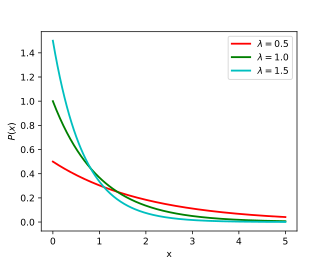
\includegraphics[
                width=\linewidth,
                height=5cm,
                keepaspectratio,
            ]{images/distributions/Exponential_distribution_pdf_-_public_domain.svg.png}
            \caption{Exponential Distribution: PDF \cite{wiki/Exponential_distribution}}
        \end{figure}
    \end{minipage}
    \hfill
    \begin{minipage}{0.45\linewidth}
        \begin{figure}[H]
            \centering
            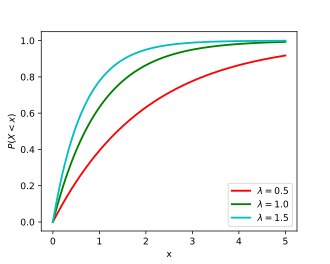
\includegraphics[
                width=\linewidth,
                height=5cm,
                keepaspectratio,
            ]{images/distributions/Exponential_distribution_cdf_-_public_domain.svg.png}
            \caption{Exponential Distribution: CDF \cite{wiki/Exponential_distribution}}
        \end{figure}
    \end{minipage}
    \hfill
\end{table}



\subsection{Distribution of the Sample Statistic ($T_n$)}

\begin{enumerate}
    \item Let $X_1 , X_2, \cdots , X _n$ are i.i.d. exponentially distributed, i.e. $X _i \sim \exp(\lambda )$. 
    \hfill \cite{statistics/book/Statistics-for-Data-Scientists/Maurits-Kaptein}

    \item The exponential distribution function is given by $F (x) = 1 - \exp (-\lambda x)$ for $x > 0$ and zero otherwise. 
    \hfill \cite{statistics/book/Statistics-for-Data-Scientists/Maurits-Kaptein}
\end{enumerate}

\subsubsection{Distribution of the Sample Minimum ($T_n = F _{X_{(1)}}$)}

\begin{enumerate}
    \item $F _{X_{(1)}} (x) = 1 - \exp (-n\lambda x)$ for $x > 0$ and zero otherwise
    \hfill \cite{statistics/book/Statistics-for-Data-Scientists/Maurits-Kaptein}

    \item Thus this implies that the sample distribution of the minimum $X_{(1)}$ is exponentially distributed, $X_{(1)} \sim \exp (n\lambda)$, but now with parameter $n\lambda$, when $X_1 ,X_2, \cdots , X _n$ are i.i.d. $\exp(\lambda)$ distributed.
    \hfill \cite{statistics/book/Statistics-for-Data-Scientists/Maurits-Kaptein}
\end{enumerate}



\subsection{Summary}

\begin{enumerate}
    \item \textbf{Parameters}: ${\displaystyle \lambda >0}$ (rate or inverse scale)
    \hfill \cite{wiki/Exponential_distribution, statistics/book/Statistics-for-Data-Scientists/Maurits-Kaptein}

    \item \textbf{Support}: ${\displaystyle x\in [0,\infty )}$
    \hfill \cite{wiki/Exponential_distribution, statistics/book/Statistics-for-Data-Scientists/Maurits-Kaptein}

    \item \textbf{PDF}:
    ${\displaystyle \lambda e^{-\lambda x}}$
    \hfill \cite{wiki/Exponential_distribution, statistics/book/Statistics-for-Data-Scientists/Maurits-Kaptein}

    \item \textbf{CDF}: ${\displaystyle 1-e^{-\lambda x}}$
    \hfill \cite{wiki/Exponential_distribution}

    \item \textbf{Quantile}: ${\displaystyle -{\dfrac {\ln(1-p)}{\lambda }}}$
    \hfill \cite{wiki/Exponential_distribution}

    \item \textbf{Mean}: $\dfrac{1}{\lambda}$
    \hfill \cite{wiki/Exponential_distribution}

    \item \textbf{Median}: $\dfrac{\ln(2)}{\lambda}$
    \hfill \cite{wiki/Exponential_distribution}

    \item \textbf{Mode}: $0$
    \hfill \cite{wiki/Exponential_distribution}

    \item \textbf{Variance}: $\dfrac{1}{\lambda^2}$
    \hfill \cite{wiki/Exponential_distribution}

    \item \textbf{Skewness}: $2$
    \hfill \cite{wiki/Exponential_distribution}

    \item \textbf{Excess kurtosis}: $6$
    \hfill \cite{wiki/Exponential_distribution}

    \item \textbf{Entropy}: $1-\ln(\lambda)$
    \hfill \cite{wiki/Exponential_distribution}

    \item \textbf{Fisher information}: $\dfrac{1}{\lambda^2}$
    \hfill \cite{wiki/Exponential_distribution}

    \item \textbf{Expected shortfall}:
    $
        {\displaystyle {\dfrac {-\ln(1-p)+1}{\lambda }}}
    $
    \hfill \cite{wiki/Exponential_distribution}

    \item \textbf{Moment-generating function (MGF)}:
    $
        {\displaystyle {\dfrac {\lambda }{\lambda -t}},{\text{ for }}t<\lambda }
    $
    \hfill \cite{wiki/Exponential_distribution}

    \item \textbf{Characteristic function (CF)}:
    $
        {\displaystyle {\dfrac {\lambda }{\lambda -it}}}
    $
    \hfill \cite{wiki/Exponential_distribution}

    \item \textbf{Kullback–Leibler divergence}:
    $
        {\displaystyle \ln {\dfrac {\lambda _{0}}{\lambda }}+{\dfrac {\lambda }{\lambda _{0}}}-1}
    $
    \hfill \cite{wiki/Exponential_distribution}
\end{enumerate}






















\section{Laplace distribution/ Double Exponential Distribution ( $ {\displaystyle \text {Laplace} (\mu ,b)} $ )}


\begin{table}[H]
    \hfill
    \begin{minipage}{0.45\linewidth}
        \begin{figure}[H]
            \centering
            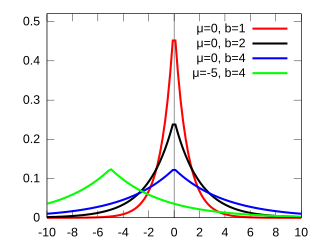
\includegraphics[
                width=\linewidth,
                height=5cm,
                keepaspectratio,
            ]{images/distributions/Laplace_pdf_mod.svg.png}
            \caption{Double Exponential/ Laplace Distribution: PDF \cite{wiki/Laplace_distribution}}
        \end{figure}
    \end{minipage}
    \hfill
    \begin{minipage}{0.45\linewidth}
        \begin{figure}[H]
            \centering
            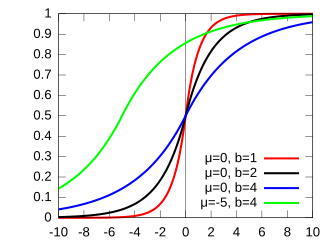
\includegraphics[
                width=\linewidth,
                height=5cm,
                keepaspectratio,
            ]{images/distributions/Laplace_cdf_mod.svg.png}
            \caption{Double Exponential/ Laplace Distribution: CDF \cite{wiki/Laplace_distribution}}
        \end{figure}
    \end{minipage}
    \hfill
\end{table}



\subsection{PDF}

\begin{enumerate}
    \item The double exponential is symmetric, like the normal PDF
    \hfill \cite{statistics/book/Statistics-for-Data-Scientists/Maurits-Kaptein}

    \item The double exponential PDF can easily be determined using the exponential PDF. 
    The double exponential PDF, for any value $x \in \mathbb{R}$, is defined by $0.5 f_\lambda (\dabs{x})$, with $\dabs{\cdot}$ the absolute function.
    \hfill \cite{statistics/book/Statistics-for-Data-Scientists/Maurits-Kaptein}
    \\
    Note: $\mu = 0, b=\dfrac{1}{\lambda}$
    \hfill \cite{common/online/chatgpt}
\end{enumerate}




\subsection{Summary}

\begin{enumerate}
    \item \textbf{Parameters}:
    \hfill \cite{wiki/Laplace_distribution}
    \begin{enumerate}
        \item ${\displaystyle \mu }$ location (real)
        \hfill \cite{wiki/Laplace_distribution}
        
        \item ${\displaystyle b>0}$ scale (real)
        \hfill \cite{wiki/Laplace_distribution}
    \end{enumerate}

    \item \textbf{Support}: $ {\displaystyle \mathbb {R} }$
    \hfill \cite{wiki/Laplace_distribution, statistics/book/Statistics-for-Data-Scientists/Maurits-Kaptein}

    \item \textbf{PDF}:
    $ {\displaystyle {\dfrac {1}{2b}}\exp \left(-{\dfrac {|x-\mu |}{b}}\right)}$
    \hfill \cite{wiki/Laplace_distribution, statistics/book/Statistics-for-Data-Scientists/Maurits-Kaptein}

    \item \textbf{CDF}: $ {\displaystyle {\begin{cases}{\dfrac {1}{2}}\exp \left({\dfrac {x-\mu }{b}}\right)&{\text{if }}x\leq \mu \\[8pt]1-{\dfrac {1}{2}}\exp \left(-{\dfrac {x-\mu }{b}}\right)&{\text{if }}x\geq \mu \end{cases}}}$
    \hfill \cite{wiki/Laplace_distribution}

    \item \textbf{Quantile}: $ {\displaystyle {\begin{cases}\mu +b\ln \left(2F\right)&{\text{if }}F\leq {\dfrac {1}{2}}\\[8pt]\mu -b\ln \left(2-2F\right)&{\text{if }}F\geq {\dfrac {1}{2}}\end{cases}}}$
    \hfill \cite{wiki/Laplace_distribution}

    \item \textbf{Mean}: $ {\displaystyle \mu }$
    \hfill \cite{wiki/Laplace_distribution}

    \item \textbf{Median}: $ {\displaystyle \mu }$
    \hfill \cite{wiki/Laplace_distribution}

    \item \textbf{Mode}: $ {\displaystyle \mu }$
    \hfill \cite{wiki/Laplace_distribution}

    \item \textbf{Variance}: $ {\displaystyle 2b^{2}}$
    \hfill \cite{wiki/Laplace_distribution}

    \item \textbf{Skewness}: $ {\displaystyle 0}$
    \hfill \cite{wiki/Laplace_distribution}

    \item \textbf{Excess kurtosis}: $  {\displaystyle 3} $
    \hfill \cite{wiki/Laplace_distribution}

    \item \textbf{Entropy}: $  {\displaystyle \log(2be)} $
    \hfill \cite{wiki/Laplace_distribution}

    % \item \textbf{Fisher information}: $ $
    % \hfill \cite{wiki/Laplace_distribution}

    \item \textbf{Expected shortfall}:
    $ {\displaystyle {\begin{cases}\mu +b\left({\dfrac {p}{1-p}}\right)(1-\ln(2p))&,p<0.5\\\mu +b\left(1-\ln \left(2(1-p)\right)\right)&,p\geq 0.5\end{cases}}}$
    \hfill \cite{wiki/Laplace_distribution}

    \item \textbf{Moment-generating function (MGF)}: 
    $ {\displaystyle {\dfrac {\exp(\mu t)}{1-b^{2}t^{2}}}{\text{ for }}|t|<1/b}$
    \hfill \cite{wiki/Laplace_distribution}

    \item \textbf{Characteristic function (CF)}:
    $ {\displaystyle {\dfrac {\exp(\mu it)}{1+b^{2}t^{2}}}}$
    \hfill \cite{wiki/Laplace_distribution}

    \item \textbf{Kullback–Leibler divergence}:
    $ $
    \hfill \cite{wiki/Laplace_distribution}

    \item \textbf{Median absolute deviation (MAD)}:
    $ {\displaystyle b\ln 2}$
    \hfill \cite{wiki/Laplace_distribution}
\end{enumerate}























\chapter{Relationships Between Distributions}

\section{Binomial-Poisson}

\begin{enumerate}
    \item The Poisson and binomial distribution functions are quite close whenever $\lambda$ is equal to $np$ and $n$ is relatively large. 
    \hfill \cite{statistics/book/Statistics-for-Data-Scientists/Maurits-Kaptein}

    \item It can be shown that the Poisson probabilities are the limit of the binomial probabilities when $n$ converges to infinity under the condition that $np$ converges to $\lambda$.
    \hfill \cite{statistics/book/Statistics-for-Data-Scientists/Maurits-Kaptein}
\end{enumerate}



\section{Binomial-Normal}

\begin{enumerate}
    \item Probability calculation with the binomial distribution function can be adequately approximated with a normal distribution function when the mean $np$ and the value $n (1 - p)$ are both larger than $5$ and the sample size is at least $20$ ($n \geq 20$).
    \hfill \cite{statistics/book/Statistics-for-Data-Scientists/Maurits-Kaptein}
\end{enumerate}


















\chapter{Decisions in Uncertainty}


\section{Bootstrapping}

\begin{enumerate}
    \item  The bootstrap provides a very general way to obtain a quantification of the uncertainty of an estimator.
    \hfill \cite{statistics/book/Statistics-for-Data-Scientists/Maurits-Kaptein}

    \item a larger sample decreases the variance of an estimator (i.e., the estimator becomes more precise).
    \hfill \cite{statistics/book/Statistics-for-Data-Scientists/Maurits-Kaptein}

    \item when estimating a population mean or difference in population means, we find that a smaller population variance leads to a smaller variance of the estimator.
    \hfill \cite{statistics/book/Statistics-for-Data-Scientists/Maurits-Kaptein}

    \item  The bootstrap has these exact same properties and is easy to carry out for many sample statistics; it provides a first entry into making decisions regarding populations based on sample data.
    \hfill \cite{statistics/book/Statistics-for-Data-Scientists/Maurits-Kaptein}

    \item  informally, it is quite clear that a large random sample and a relatively small variance of the estimator $\hat{\theta}$ should both increase our confidence regarding statements we can make about the population.
    \hfill \cite{statistics/book/Statistics-for-Data-Scientists/Maurits-Kaptein}

\end{enumerate}

\subsection{Basic Idea of Bootstrap}

\begin{enumerate}
    \item Given a (random) sample of size n from some population with distribution function $F_X$ , we frequently set out to obtain an estimate of a population parameter $\theta = T (x)$.
    \hfill \cite{statistics/book/Statistics-for-Data-Scientists/Maurits-Kaptein}

    \item Our point estimate of the parameter of interest is often what is called the “plug-in estimator” for $\theta$: $\hat{\theta} = T (x_1, \cdots , x_n )$; i.e., it is the statistic of interest calculated on the sample data $x_1, \cdots , x_n$ .
    \hfill \cite{statistics/book/Statistics-for-Data-Scientists/Maurits-Kaptein}

    \item we are interested in the distribution function of $\hat{\theta}$ over repeated samples.
    We are interested in $F_{\hat{\theta}}$ as it gives us information about the variability of our estimate over repeated samples.
    Depending on the statistic involved, the sampling plan, and the assumptions one is willing to make about $F_X$ or $f_X$ , we might be able to analytically derive $F_{\hat{\theta}}$.
    However, obtaining $F_{\hat{\theta}}$ in general (or properties thereof) can be challenging.
    \hfill \cite{statistics/book/Statistics-for-Data-Scientists/Maurits-Kaptein}

    \item The bootstrap addresses the problem of deriving $F_{\hat{\theta}}$ using the power of computer simulation.
    \hfill \cite{statistics/book/Statistics-for-Data-Scientists/Maurits-Kaptein}

    \item if we have a good estimate of the population distribution function $F_X$ , i.e., $\hat{F}_X$ , we can simply program a computer to obtain $M$ samples (by \textbf{simulation}) of size $n$ from $\hat{F}_X$ using the same sampling plan that we have used to collect our initial sample.
    If $\hat{F}_X$ is close to $F_X$ it does not really matter if we draw from $\hat{F}_X$ or $F_X$ .
    As long as our estimate of $\hat{F}_X$ is close to the true $F_X$ , our samples of $\hat{F}_{\hat{\theta}}$ can be used to approximate properties of $F_{\hat{\theta}}$
    \hfill \cite{statistics/book/Statistics-for-Data-Scientists/Maurits-Kaptein}

    \item On each sample $m = 1, \cdots , M$ we can subsequently compute the statistic of interest, $\hat{\theta}^{(1)} , \cdots , \hat{\theta}^{(M)}$ which themselves serve as approximate samples from $F_{\hat{\theta}}$ (approximate as we are using $\hat{F}_X $, and thus we obtain samples from $\hat{F}_{\hat{\theta}}$).
    \hfill \cite{statistics/book/Statistics-for-Data-Scientists/Maurits-Kaptein}

    \item standard error of a statistic can simply be computed by computing the standard deviation of the M samples of the statistic of interest
    $
        \hat{SE}(\hat{\theta})
        = \sqrt{\dfrac{\dsum^M_{m=1} \dParenBrac{\hat{\theta}^{(m)}-\bar{\theta}}^2}{M-1}}
    $
    where
    $
        \bar{\theta} = \dfrac{1}{M} \dsum^M_{m=1} \hat{\theta}^{(m)}
    $
    \hfill \cite{statistics/book/Statistics-for-Data-Scientists/Maurits-Kaptein}

    \item we are interested in the variability of our estimator over differently obtained samples, we should adopt our bootstrapping procedure accordingly.
    \hfill \cite{statistics/book/Statistics-for-Data-Scientists/Maurits-Kaptein}

    \item Although the bootstrap is appealing as it allows one to quantify the uncertainty for virtually any statistic—by simply replacing tedious analytical work with simple computer operations—one should always be careful: for complex sampling schemes and complex population distributions, $\hat{F}_X$ , or the resulting $M$ bootstrap samples of the statistic of interest, might not provide a good quantification of the uncertainty associated with $\hat{\theta}$.
    \hfill \cite{statistics/book/Statistics-for-Data-Scientists/Maurits-Kaptein}

    \item We can use $\hat{F}_X$ , in combination with computer simulation, to generate bootstrap samples $m = 1, \cdots , M$ and compute $\hat{\theta}(m)$ for arbitrary statistics $T $.
    \hfill \cite{statistics/book/Statistics-for-Data-Scientists/Maurits-Kaptein}

    \item \textbf{Steps}:
    \begin{enumerate}
        \item we estimate $F_X$ based using our sample $x_1, \cdots , x_n$ . This gives us $\hat{F}_X $.
        \hfill \cite{statistics/book/Statistics-for-Data-Scientists/Maurits-Kaptein}

        \item we obtain $M$ random samples from $\hat{F}_X$ (each of size $n$), on which we computed our bootstrap estimates of the statistic of interest $\hat{\theta}^{(1)} , \cdots, \hat{\theta}^{(M)}$ which we regard as (approximate) samples from $F_{\hat{\theta}}$.
        \hfill \cite{statistics/book/Statistics-for-Data-Scientists/Maurits-Kaptein}
    \end{enumerate}

    \item \textbf{Disadvantages}:
    \begin{enumerate}
        \item it might be the case that $\hat{F}_X$ is a very poor estimate of $F_X$ .
        This is often the case when $n$ is small, but it might also be caused by the fact that the original sample $x_1, \cdots , x_n$ is not obtained through simple random sampling (resampling with replacement).
        If the latter is the case, the sampling scheme that was used should be taken into consideration when computing $\hat{F}_X$.
        \hfill \cite{statistics/book/Statistics-for-Data-Scientists/Maurits-Kaptein}

        \item the sampling scheme implemented in the second step (resampling step) should mimic the sampling scheme that was originally used: if the $M$ bootstrap samples are generated using a different sampling scheme than the sampling scheme of interest, $F_{\hat{\theta}}$ might not be properly approximated by the M bootstrap samples.
        \hfill \cite{statistics/book/Statistics-for-Data-Scientists/Maurits-Kaptein}

        \item While the bootstrap provides an easy way of quantifying uncertainty that we can use to make decisions, it is hard in general to make statements about the \textbf{quality} of these decisions.
        \hfill \cite{statistics/book/Statistics-for-Data-Scientists/Maurits-Kaptein}
    \end{enumerate}

\subsubsection{Non-Parametric Bootstrap}

    \item no parametric assumptions regarding $F_X$ are made in this procedure
    \hfill \cite{statistics/book/Statistics-for-Data-Scientists/Maurits-Kaptein}

    \item  The simplest bootstrap approach for obtaining $\hat{F}_X$ is to simply use the empirical distribution function: the original samples $x_1, \cdots , x_n$ in our sample can be used to construct a discrete approximation of $F_X$ by simply giving each unique value $v_i$ in $x_1, \cdots , x_n$ probability $\dfrac{1}{n}$ .
    \hfill \cite{statistics/book/Statistics-for-Data-Scientists/Maurits-Kaptein}

\subsubsection{Parametric Bootstrap}

    \item in the parametric bootstrap $\hat{F}_X$ is assumed to be of a certain form (e.g., it is assumed to be normal), and plug-in estimates for its parameters (e.g., $\hat{\mu}$ and $\hat{\sigma}^2$ in the normal case) are used to estimate $F_X$ .
    \hfill \cite{statistics/book/Statistics-for-Data-Scientists/Maurits-Kaptein}

    \item If the assumptions are correct, the parametric bootstrap is preferable over the non-parametric bootstrap.
    \hfill \cite{statistics/book/Statistics-for-Data-Scientists/Maurits-Kaptein}

\end{enumerate}






\section{Hypothesis testing}

\begin{enumerate}
    % \item  make binary decisions
    % \hfill \cite{statistics/book/Statistics-for-Data-Scientists/Maurits-Kaptein}

    \item \textbf{Test Statistics} ($t$): A single number that summarizes the sample data used to conduct the test hypothesis.
    \hfill \cite{ctl.unm.edu/assets/docs/resources/hypothesis-testing-sheet.pdf}

    \item $p$-\textbf{value}: Probability of observing a test statistics.
    \hfill \cite{ctl.unm.edu/assets/docs/resources/hypothesis-testing-sheet.pdf}


    \item without making any assumptions regarding the sampling process and/or the population distributions involved, it is practically impossible to say anything about the population based on sample data with full certainty.
    \hfill \cite{statistics/book/Statistics-for-Data-Scientists/Maurits-Kaptein}

    \item Hypothesis testing provides a method for making binary decisions that, in many instances, does give us clear quantitative statements about the quality of the decisions we make.
    \hfill \cite{statistics/book/Statistics-for-Data-Scientists/Maurits-Kaptein}

    \item Within hypothesis testing the general setup is as follows: we state our decision problem as a choice between two competing hypotheses regarding the population, often called the \textbf{null hypothesis} $H_0 $, and the \textbf{alternative hypothesis} $H_a $.
    Given that $H_0$ and $H_a$ are complementary, one of the two \textbf{must} be true in the population.
    \hfill \cite{statistics/book/Statistics-for-Data-Scientists/Maurits-Kaptein}
    \begin{enumerate}
        \item \textbf{Null Hypothesis} ($H_0$): A statement of no change and is 0 assumed true until evidence indicates otherwise.
        \hfill \cite{ctl.unm.edu/assets/docs/resources/hypothesis-testing-sheet.pdf}

        \item \textbf{Alternate Hypothesis} ($H_a$): A statement that the researcher is trying to find evidence to support
        \hfill \cite{ctl.unm.edu/assets/docs/resources/hypothesis-testing-sheet.pdf}
    \end{enumerate}

    \item The subsequent rationale of hypothesis testing is that we assume that the null hypothesis is true and that we gather \textbf{sufficient evidence} to demonstrate that it is not true.
    It defines sufficient evidence such that the probability of making a type 1 error is \textbf{at most} $\alpha$.
    The level $\alpha$ is called the \textbf{significance level} and it is the maximal allowable probability of rejecting the null hypothesis when the null hypothesis is actually true.
     It is often set equal to a value of $\alpha = 0.05$ or $\alpha = 0.01$.
    \hfill \cite{statistics/book/Statistics-for-Data-Scientists/Maurits-Kaptein}

    \item  Thus the \textbf{goal} of hypothesis testing is to \textbf{reject the null hypothesis} on the basis of sufficient and well-collected data.
    We will decide that either $H_0$ is rejected (thus $H_a$ must be true) or is not rejected (thus there is no or not enough evidence to demonstrate that $H_0$ is false).
    \hfill \cite{statistics/book/Statistics-for-Data-Scientists/Maurits-Kaptein}


\begin{figure}[H]
    \centering
    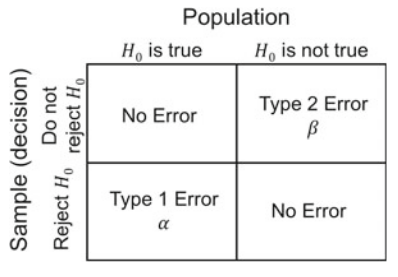
\includegraphics[
        width=\linewidth,
        height=5cm,
        keepaspectratio,
    ]{images/statistics/hypothesis-testing-errors.png}
    \caption{
        Types of errors in hypothesis testing
        \cite{statistics/book/Statistics-for-Data-Scientists/Maurits-Kaptein}
    }
\end{figure}

    \item 4 situations:
    \begin{enumerate}
        \item {[\textbf{true positive}]} we do not reject $H_0$ when $H_0$ is true in the population
        \hfill \cite{statistics/book/Statistics-for-Data-Scientists/Maurits-Kaptein}

        \item {[\textbf{true negative}]} we reject $H_0 $, and subsequently accept $H_a $, when $H_a$ is true in the population
        \hfill \cite{statistics/book/Statistics-for-Data-Scientists/Maurits-Kaptein}

        \item {[\textbf{false positive}]} we reject $H_0$ while in reality it is true, aka false positive or type 1 error.
        The probability of a type 1 error is associated with the level $\alpha$.
        The $\alpha$ is used as a maximal allowable type 1 error for a decision rule.
        \hfill \cite{statistics/book/Statistics-for-Data-Scientists/Maurits-Kaptein}

        \item {[\textbf{false negative}]} we do not reject $H_0$ , while in actuality $H_a$ is true, aka type 2 error.
        The probability of a type 2 error is associated with the level $\beta$.
        The value $\beta$ is used a maximal allowable type 2 error.
        One minus the type 2 error ($1-\beta$) is called the \textbf{power} of the binary decision rule.
        It indicates how likely the null hypothesis is rejected when the alternative hypothesis is true.
        \hfill \cite{statistics/book/Statistics-for-Data-Scientists/Maurits-Kaptein}
    \end{enumerate}

    \item it is easy to create a decision procedure that has a type 1 error probability equal to zero:
    if we simply never reject $H_0$ —in this case basically we state that there is never sufficient evidence to reject $H_0$ —we will never make a type 1 error.
    While this decision procedure does control the type 1 error, it is clearly not very useful, as the power of this decision rule is zero: we never accept the alternative hypothesis when it is true.
    \hfill \cite{statistics/book/Statistics-for-Data-Scientists/Maurits-Kaptein}

    \item the procedure of hypothesis testing aims to be less conservative (e.g., it will reject the null hypothesis sometimes but not too often when it would be true).
    \hfill \cite{statistics/book/Statistics-for-Data-Scientists/Maurits-Kaptein}

    \item \textbf{One tailed test}: Test statistics falls into one specified tail of its sampling distribution
    \hfill \cite{ctl.unm.edu/assets/docs/resources/hypothesis-testing-sheet.pdf}

    \item \textbf{Two tailed test}: Test statistics can falling into either tail of its sampling distribution
    \hfill \cite{ctl.unm.edu/assets/docs/resources/hypothesis-testing-sheet.pdf}

    \item Steps to Significance Testing:
    \hfill \cite{ctl.unm.edu/assets/docs/resources/hypothesis-testing-sheet.pdf}
    \begin{enumerate}
        \item Define $H_0$ and $H_a$
        \hfill \cite{ctl.unm.edu/assets/docs/resources/hypothesis-testing-sheet.pdf}

        \item Identify test, $\alpha$, find critical value, test statistics
        \hfill \cite{ctl.unm.edu/assets/docs/resources/hypothesis-testing-sheet.pdf}

        \item Construct acceptance/rejection regions
        \hfill \cite{ctl.unm.edu/assets/docs/resources/hypothesis-testing-sheet.pdf}

        \item Calculate test statistics
        \hfill \cite{ctl.unm.edu/assets/docs/resources/hypothesis-testing-sheet.pdf}

        \begin{enumerate}
            \item Critical value approach: Determine critical region
            \hfill \cite{ctl.unm.edu/assets/docs/resources/hypothesis-testing-sheet.pdf}

            \item p-value approach: Calculate p-value
            \hfill \cite{ctl.unm.edu/assets/docs/resources/hypothesis-testing-sheet.pdf}
        \end{enumerate}

        \item Retain or reject the hypothesis
        \hfill \cite{ctl.unm.edu/assets/docs/resources/hypothesis-testing-sheet.pdf}
    \end{enumerate}

    \item \textbf{Choosing a Statistical Test}:

\begin{figure}[H]
    \centering
    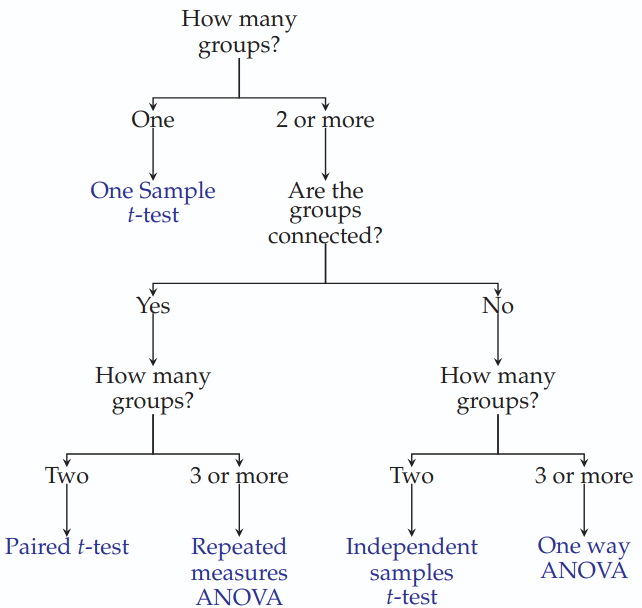
\includegraphics[
        width=\linewidth,
        height=7cm,
        keepaspectratio,
    ]{images/statistics/hypothesis-testing-desicion-tree.png}
    \caption{
        Choosing a Statistical Test: Decision Tree
        \cite{ctl.unm.edu/assets/docs/resources/hypothesis-testing-sheet.pdf}
    }
\end{figure}

    \begin{enumerate}
        \item Categorical Data: Use Chi Square
        \hfill \cite{ctl.unm.edu/assets/docs/resources/hypothesis-testing-sheet.pdf}

        \item Sample size ($n$):
        \begin{enumerate}
            \item $n < 30$ and Population Variance is unknown - t-test
            \hfill \cite{ctl.unm.edu/assets/docs/resources/hypothesis-testing-sheet.pdf}

            \item $n < 30$ and Population Variance is known - z-test
            \hfill \cite{ctl.unm.edu/assets/docs/resources/hypothesis-testing-sheet.pdf}

            \item $n > 30$ - z-test or t-test
            \hfill \cite{ctl.unm.edu/assets/docs/resources/hypothesis-testing-sheet.pdf}
        \end{enumerate}
    \end{enumerate}

    \item The z-test heavily depends on asymptotic theory and therefore requires \textbf{large sample sizes}.
    \hfill \cite{statistics/book/Statistics-for-Data-Scientists/Maurits-Kaptein}

    \item the t-test can be used for small sample sizes but under the strict assumption of having collected data from a \textbf{normal distribution}.
    \hfill \cite{statistics/book/Statistics-for-Data-Scientists/Maurits-Kaptein}

    \item Alternative approaches for the z-test and t-test have been developed that require fewer or no assumptions. These tests are referred to as \textbf{non-parametric tests}.
    \hfill \cite{statistics/book/Statistics-for-Data-Scientists/Maurits-Kaptein}

    \item The term \textbf{heteroskedasticity} refers to differences in variation or variability. 
    In hypothesis testing this is often translated to a hypothesis on the variances or standard deviations from two different populations, as we described for the two samples t-test.
    Under the assumption of normality the most efficient test statistic (F-test) is based on a ratio of the two sample variances, but under non-normal data an alternative approach (Levene’s test) has been suggested. 
    \hfill \cite{statistics/book/Statistics-for-Data-Scientists/Maurits-Kaptein}

    \item The common practice of testing the (two-sided) null hypothesis has a few \textbf{drawbacks}.
    \hfill \cite{statistics/book/Statistics-for-Data-Scientists/Maurits-Kaptein}
    \begin{enumerate}
        \item For (extremely) large samples we will almost always reject the null hypothesis. 
        This might not be desirable, as rejecting the null hypothesis in such cases does not actually imply that the (e.g.,) difference in means of interest is indeed large. 
        \hfill \cite{statistics/book/Statistics-for-Data-Scientists/Maurits-Kaptein}
        
        \item Not rejecting the null hypothesis $H_0 : \mu( f ) = \mu_0$ is no proof that the null hypothesis is true.
        It is very easy not to reject the null hypothesis: you just need to collect as little information as possible. 
        If we would collect only a few observations the confidence interval would be very wide and the value $\mu_0$ is likely to fall inside this wide confidence interval, but this does not guarantee that $\mu( f ) = \mu_0$ or even close to it.
        \hfill \cite{statistics/book/Statistics-for-Data-Scientists/Maurits-Kaptein}
    \end{enumerate}
    One way of dealing with these two issues on hypothesis testing is to reduce the significance level $\alpha$ to a much lower value than the commonly used $\alpha = 0.05$. 
    We may use $\alpha = 0.001$ or even $\alpha = 0.0001$ to make the hypothesis statements more confident than just $95\%$. 
    \hfill \cite{statistics/book/Statistics-for-Data-Scientists/Maurits-Kaptein}
\end{enumerate}


\begin{figure}[H]
    \centering
    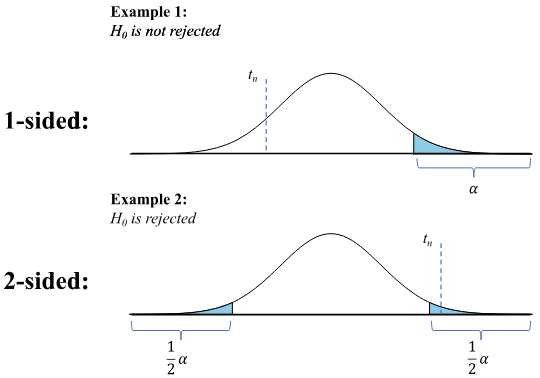
\includegraphics[
        width=\linewidth,
        height=5.5cm,
        keepaspectratio,
    ]{images/statistics/one-sided_two-sided_t-test.png}
\end{figure}

The difference between one-sided and two-sided tests.
In both cases $H_0$ is not rejected if the observed test statistic $t_n$ falls outside of the rejection region $\alpha$.
However, for a one-sided test (top) the rejection region is located on one tail of the distribution (the blue area denoted $\alpha$).
Hence, only if $t_n > z_{1-\alpha}$ (in this case), and sufficiently large to fall within the rejection region, is $H_0$ rejected.
For a two-sided test the rejection region is split over the two tails of the distribution: hence $H_0$ can be rejected if $t_n$ is either sufficiently small or sufficiently large.
Finally, note that if $t_n > z_{1-\alpha}$—if this is the direction of the one-sided test—a one-sided test might reject $H_0 $, whereas the same $t_n$ might not lead to a rejection in the two-sided case, because the critical value for the two-sided test is larger than for the one-sided test
\hfill \cite{statistics/book/Statistics-for-Data-Scientists/Maurits-Kaptein}

















\subsection{The One-Sided $z$-Test for a Single Mean ($H_0:\mu(f) \leq \mu_0$)}

\begin{enumerate}
    \item hypothesis on the population mean: $H_0 : \mu( f ) \leq \mu_0$ versus $H_a : \mu( f ) > \mu_0 $.
    \hfill \cite{statistics/book/Statistics-for-Data-Scientists/Maurits-Kaptein}

    \item we assume that the sample is large enough to be able to use the normal distribution function as an approximation to the distribution function of the statistic that we are using to make a decision about the null hypothesis
    \hfill \cite{statistics/book/Statistics-for-Data-Scientists/Maurits-Kaptein}

    \item Let’s assume that we have collected a random sample $Y_1 , Y_2, \cdots , Y_n$ from the population.
    We may estimate the population mean $\mu ( f )$ with the sample average $\bar{Y}$ .
    \hfill \cite{statistics/book/Statistics-for-Data-Scientists/Maurits-Kaptein}

    \item when $\bar{Y}$ is smaller or equal to $\mu_0$ the random variable $\bar{Y}$ seems to be in line with the null hypothesis $H_0 : \mu( f ) \leq \mu_0$ .
    In other words, there is no evidence that the \textbf{null hypothesis is false}.
    \hfill \cite{statistics/book/Statistics-for-Data-Scientists/Maurits-Kaptein}

    \item Although the random variable does not suggest any conflict with the null hypothesis $H_0 : \mu( f ) \leq \mu_0 $, it \textbf{does not guarantee} that $\mu( f ) \leq \mu_0$ either.
    \hfill \cite{statistics/book/Statistics-for-Data-Scientists/Maurits-Kaptein}

    \item If the population mean $\mu( f )$ were somewhat larger than $\mu_0 $, it might not be completely unlikely to observe a sample average still below $\mu_0$ due to the sampling (a type 2 error).
    \hfill \cite{statistics/book/Statistics-for-Data-Scientists/Maurits-Kaptein}

    \item When $\bar{Y}$ is larger than $\mu_0 $, we might start to believe that the null hypothesis is incorrect.
    However, when $\bar{Y}$ is just a little higher than $\mu_0$ this might not be very unlikely either, even when $\mu( f ) \leq \mu_0$ .
    \hfill \cite{statistics/book/Statistics-for-Data-Scientists/Maurits-Kaptein}

    \item For instance, for any symmetric $f$ at $\mu( f ) = \mu_0 $, the probability that $\bar{Y}$ is larger than $\mu_0$ is equal to $0.5$.
    Only when the sample average $\bar{Y}$ is substantially larger—thus when there is sufficient evidence—than $\bar{Y}$ would we start to indicate that the null hypothesis $H_0 : \mu( f ) \leq \mu_0$ is unlikely to be true (although a type 1 error could be made here).
    \hfill \cite{statistics/book/Statistics-for-Data-Scientists/Maurits-Kaptein}

    \item we want to find a criterion for the average $\bar{Y}$ such that the average can only be larger than this criterion with a probability that is at most equal to $\alpha$ when the null hypothesis is true.
    If we assume that this criterion is equal to $\mu_0 + \delta$, with $\delta > 0$, then the probability that $\bar{Y}$ is larger than $\mu_0 + \delta$ is given by
    \hfill \cite{statistics/book/Statistics-for-Data-Scientists/Maurits-Kaptein}
    \\[0.3cm]
    .\hfill
    $
        P( \bar{Y} > \mu _0 + \delta)
        = P\dParenBrac{\dfrac{ ( \bar{Y} - \mu ( f ))}{\sigma( f )/\sqrt{n}} > \dfrac{\mu _0 - \mu ( f ) + \delta}{\sigma/\sqrt{n}}}
        \approx 1 - \Phi\dParenBrac{\dfrac{\mu _0 - \mu ( f ) + \delta}{\sigma( f )/\sqrt{n}}}
    $
    \hfill \cite{statistics/book/Statistics-for-Data-Scientists/Maurits-Kaptein}
    \\[0.3cm]
    where $\Phi$ is the standard normal PDF.
    \hfill \cite{statistics/book/Statistics-for-Data-Scientists/Maurits-Kaptein}

    \item Under the null hypothesis $H_0 : \mu( f ) \leq \mu_0$ this probability is the type 1 error and it is maximized when $\mu( f ) = \mu_0$ .
    \hfill \cite{statistics/book/Statistics-for-Data-Scientists/Maurits-Kaptein}

    \item if we deliberately set $\mu( f ) = \mu_0$ to maximize the type 1 error, the probability $P ( \bar{Y} > \mu_0 + \delta)$ is given by $1 - \Phi(\delta\sqrt{n}/\sigma)$.
    \hfill \cite{statistics/book/Statistics-for-Data-Scientists/Maurits-Kaptein}

    \item When we choose $\delta$ equal to $\delta = \dfrac{z_{1-\alpha} \sigma( f )}{\sqrt{n}}$, the probability becomes $P ( \bar{Y} > \mu_0 + \delta) \approx \alpha$.
    When $\bar{Y} > \mu_0 + \dfrac{z_{1 - \alpha} \sigma( f )}{\sqrt{n}}$ the probability of rejecting the null hypothesis is at most $\alpha$—and hence we have defined sufficient evidence by the criterion $\mu0 + \dfrac{z_{1 - \alpha} \sigma( f )}{\sqrt{n}}$ for the null hypothesis $H_0 : \mu( f ) \leq \mu_0$ using the statistic $\bar{Y} $.
    \hfill \cite{statistics/book/Statistics-for-Data-Scientists/Maurits-Kaptein}

    \item The null hypothesis could still be true, but that it is just bad luck to have observed such an unlikely large average under the null hypothesis.
    However, we know that this probability of having bad luck is less than or equal to $\alpha$ and therefore we accept making this potential type 1 error.
    \hfill \cite{statistics/book/Statistics-for-Data-Scientists/Maurits-Kaptein}

    \item we cannot use the criterion ¯$Y > \mu_0 + \dfrac{z_{1-\alpha} \sigma( f )}{\sqrt{n}}$ directly, as it depends on the population standard deviation $\sigma( f )$, which is generally not known.
    We could estimate $\sigma( f )$ using sample standard deviation $S = \sqrt{\dfrac{1}{n-1} \dsum^n_{i=1} (Y_i - \bar{Y} )^2}$
    \hfill \cite{statistics/book/Statistics-for-Data-Scientists/Maurits-Kaptein}

    \item If the sample size is large enough, the probability $P\dParenBrac{\bar{Y} > \mu_0 + \dfrac{z_{1-\alpha} S}{\sqrt{n}}}$ would still be close to $\alpha$.
    When the sample size is large enough, we may reject the null hypothesis in practice when $\bar{Y} > \mu_0 + \dfrac{z_{1-\alpha} S}{\sqrt{n}}$ or in other words when the \textbf{asymptotic test statistic} $T_n = \dfrac{\bar{Y} - \mu_0}{S/\sqrt{n}}$ is larger than $z_{1-\alpha}$.
    \hfill \cite{statistics/book/Statistics-for-Data-Scientists/Maurits-Kaptein}

    \item For large sample sizes n, the null hypothesis $H_0 : \mu( f ) \leq \mu_0$ is tested with test statistic $T_n = \dfrac{\bar{Y} - \mu_0}{S/\sqrt{n}}$ and the null hypothesis is rejected with significance level $\alpha$ when the test statistic is larger than the critical value $z_{1-\alpha}$.
    \hfill \cite{statistics/book/Statistics-for-Data-Scientists/Maurits-Kaptein}

    \item The null hypothesis is not rejected when $T_n = \dfrac{\bar{Y} - \mu_0}{S/\sqrt{n}} \leq z_{1-\alpha}$, since there would not be enough evidence to reject the null hypothesis with significance level $\alpha$ (i.e., the observed result is not unlikely enough under $H_0 $).
    This does not mean that the null hypothesis is true.
    \hfill \cite{statistics/book/Statistics-for-Data-Scientists/Maurits-Kaptein}

    \item the asymptotic approach for testing $H_0 : \mu( f ) \leq \mu_0$ will work for most population densities $f_X$ whenever the sample size is large enough.
    \hfill \cite{statistics/book/Statistics-for-Data-Scientists/Maurits-Kaptein}

% \subsubsection{p-value}

    \item The p-value is the probability that the observed test statistic $t_n$ and more extreme observations would occur under the null hypothesis.
    \hfill \cite{statistics/book/Statistics-for-Data-Scientists/Maurits-Kaptein}
    \begin{enumerate}
        \item It measures how surprising the observed data is if the null hypothesis $H_0$ were true.
        \hfill \cite{common/online/chatgpt}

        \item A small p-value means the observed test statistic is very unlikely under $H_0 $, giving evidence against $H_0$
        \hfill \cite{common/online/chatgpt}
    \end{enumerate}

    \item Calculating p-value:
    \begin{enumerate}
        \item test statistic: $T_n = \dfrac{\bar{Y} - \mu_0}{S / \sqrt{n}}$
        \hfill \cite{common/online/chatgpt}

        \item observed test statistic: $t_n = \dfrac{\bar{Y} - \mu_0}{S / \sqrt{n}}$
        \hfill \cite{common/online/chatgpt}

        \item Convert test statistic to a probability under $H_0$
        \hfill \cite{common/online/chatgpt}
        \begin{enumerate}
            \item If $H_0$ is true, then Tn approximately follows a standard normal distribution (for large $n$).
            \hfill \cite{common/online/chatgpt}

            \item The p-value is the tail probability of seeing $t_{obs}$ or something more extreme.
            \hfill \cite{common/online/chatgpt}
        \end{enumerate}

        \item Depending on the test type:
        \hfill \cite{common/online/chatgpt}
        \begin{enumerate}
            \item Right-tailed test ($H_0:\mu\leq\mu_0$): $p=P(Z\geq t_{obs})=1-\Phi(t_{obs})$
            \hfill \cite{common/online/chatgpt}

            \item Left-tailed test ($H_0:\mu\geq\mu_0$): $p=P(Z\leq t_{obs})=\Phi(t_{obs})$
            \hfill \cite{common/online/chatgpt}

            \item Two-tailed test ($H_0:\mu= \mu_0$): $p = 2 \cdot \min(\Phi(t_{obs}), 1 - \Phi(t_{obs}))$
            \hfill \cite{common/online/chatgpt}
        \end{enumerate}
        Here $\Phi$ is the cumulative distribution function (CDF) of the standard normal.
        \hfill \cite{common/online/chatgpt}
    \end{enumerate}

\end{enumerate}




\subsection{The Two-Sided z-Test for a Single Mean ($H_0:\mu(f)=\mu_0$)}

\begin{enumerate}
    \item The null hypothesis is formulated as $H_0 : \mu( f ) = \mu_0$ and the alternative hypothesis is $H_a : \mu( f )  = \mu_0 $.
    \hfill \cite{statistics/book/Statistics-for-Data-Scientists/Maurits-Kaptein}

    \item We would reject the null hypothesis when either $T_n = \dfrac{\bar{Y} - \mu_0}{S/\sqrt{n}}$ is large positive or large negative.
    \hfill \cite{statistics/book/Statistics-for-Data-Scientists/Maurits-Kaptein}

    \item If we still keep our significance level at $\alpha$, we will reject the null hypothesis $H_0 : \mu( f )  = \mu_0$ when $\dfrac{\bar{Y} - \mu0}{S/\sqrt{n}} > z_{1-\alpha/2} $, with $z_{1-\alpha/2}$ the $1 - \alpha/2$ quantile of the standard normal distribution (when using a normal approximation), or when $\dfrac{\bar{Y} - \mu_0}{S/\sqrt{n}} < -z_{1-\alpha/2} $.
    \hfill \cite{statistics/book/Statistics-for-Data-Scientists/Maurits-Kaptein}

    \item we would reject when $\dfrac{\dabs{\bar{Y} - \mu_0}}{S/\sqrt{n}} > z_{1-\alpha/2} $, with $\dabs{x}$ the absolute value of $x$.
    \hfill \cite{statistics/book/Statistics-for-Data-Scientists/Maurits-Kaptein}

    \item we reject this hypothesis when the test statistic is sufficiently small or sufficiently large.
    \hfill \cite{statistics/book/Statistics-for-Data-Scientists/Maurits-Kaptein}

    \item To control type 1 error, we therefore split up our rejection region in two: this is why we work with $z_{1-\alpha/2}$.
    \hfill \cite{statistics/book/Statistics-for-Data-Scientists/Maurits-Kaptein}

    \item  two-sided tests, while used very often in practice, are less useful when sample sizes are very large: with a very large $n$, the standard error of a test statistic will become small, and we eventually will reject the null hypothesis in most cases.
    \hfill \cite{statistics/book/Statistics-for-Data-Scientists/Maurits-Kaptein}

    \item confidence interval contains the statistic we just discussed for hypothesis testing. 
    In the case that $\mu_0$ is not contained in the confidence interval, either $\dfrac{\bar{Y} - \mu_0}{S/\sqrt{n}} > z_{1-\alpha/2}$ or $\dfrac{\bar{Y} - \mu_0}{S/\sqrt{n}} < -z_{1-\alpha/2}$ would have occurred.
    Thus the null hypothesis $H_0 : \mu( f ) = \mu_0$ would be rejected if $\mu_0$ is not contained in $\dSquareBrac{\bar{Y} - \dfrac{z_{1-\alpha/2} S}{\sqrt{n}}, \bar{Y} + \dfrac{z_{1-\alpha/2} S}{\sqrt{n}}}$. Thus confidence intervals relate directly to two-sided hypothesis tests.
    \hfill \cite{statistics/book/Statistics-for-Data-Scientists/Maurits-Kaptein}

    \item If the null hypothesis is included in the confidence interval, we do not have sufficient evidence to reject it.
    If the confidence interval lies fully outside of the null hypothesis, there is sufficient evidence to reject the null hypothesis. 
    Theoretically (and asymptotically) using confidence intervals for testing will lead to the same type 1 error probabilities.
    \hfill \cite{statistics/book/Statistics-for-Data-Scientists/Maurits-Kaptein}

    \item The bootstrap approach is an analytical approach to obtain confidence intervals for certain statistics may be an alternative to generate confidence intervals (instead of using asymptotic theory).
    \hfill \cite{statistics/book/Statistics-for-Data-Scientists/Maurits-Kaptein}
\end{enumerate}



\subsection{Non-Parametric Test: Mann–Whitney U Test for Two Independent Samples ($H_0 : P(Y_1 > Y_2) = P(Y_1 < Y_2)$)}

\begin{enumerate}
    \item  It tests the null hypothesis $H_0 : P(Y_1 > Y_2) = P(Y_1 < Y_2)$, with $Y_1$ a random draw from the first population and $Y_2$ a random draw from the second population.
    The null hypothesis is equivalent to $H_0 : P(Y_1 > Y_2) = 0.5$.
    \hfill \cite{statistics/book/Statistics-for-Data-Scientists/Maurits-Kaptein}

    \item  If the null hypothesis is false, it is more likely to observe larger values in one of the populations with respect to the other population. 
    Thus one population is \textbf{stochastically greater} than the other population.
    \hfill \cite{statistics/book/Statistics-for-Data-Scientists/Maurits-Kaptein}

    \item If we now assume that the distribution function $F_2$ for the second population is given by $F_2(y) = F_1(y + \delta)$, with $F_1$ the distribution function of the first population and $\delta$ a (shift) parameter, the null hypothesis $H_0 : P(Y_1 > Y_2) = P(Y_1 < Y_2)$ implies that the medians of the two populations must be equal (i.e., $\delta = 0$). 
    \hfill \cite{statistics/book/Statistics-for-Data-Scientists/Maurits-Kaptein}

    \item Only in this somewhat restrictive formulation of population distributions, the Mann–Whitney U test investigates whether the two populations have equal medians.
    \hfill \cite{statistics/book/Statistics-for-Data-Scientists/Maurits-Kaptein}

    \item Mann–Whitney U test statistic: 
    \colorbox{yellow}{$
        U = 
        \dsum^{n_1} _{i=1} 
        \dsum^{n_2} _{j=1} 
        [1_{(Y_{2, j} <Y_{1,i} )} + 0.5 \cdot 1_{(Y_{1,i} =Y_{2, j} )}]
    $}
    \hfill \cite{statistics/book/Statistics-for-Data-Scientists/Maurits-Kaptein}
    \\[0.2cm]
    with $1_A$ the indicator function equal to $1$ if $A$ is true and zero otherwise.
    \hfill \cite{statistics/book/Statistics-for-Data-Scientists/Maurits-Kaptein}

    \item  It represents the number of pairs $(Y_{1,i} , Y_{2, j} )$ of observations from the two populations for which the first population provides a larger value than the second population. 
    If there are ties (i.e., $Y_{1,i} = Y_{2, j}$ ), we cannot determine which population provides the larger value; thus this pair only contributes half to the total number of observations for which the first population is larger than the second population.
    \hfill \cite{statistics/book/Statistics-for-Data-Scientists/Maurits-Kaptein}

    \item  If the variable $Y _h$ is continuous, we should not observe any ties if we use enough decimal places in the recording of the values.
    \hfill \cite{statistics/book/Statistics-for-Data-Scientists/Maurits-Kaptein}

    \item The Mann–Whitney U test only makes use of the \textbf{ordering} of the observations. 
    The total number of \textbf{pairs} for which the comparison between the two populations is made is equal to $n_1n_2 $. 
    \hfill \cite{statistics/book/Statistics-for-Data-Scientists/Maurits-Kaptein}

    \item Each observation of the first sample is compared to each observation in the second sample. 
    Thus the statistic $\dfrac{U}{n_1n_2}$ is an estimator of the probability $P(Y_1 > Y_2)$. 
    When $\dfrac{U}{n_1n_2}$ is away from $0.5$ or in other words, when U is away from $0.5n_1n_2$ , the null hypothesis $H_0 : P(Y_1 > Y_2) = 0.5$ is rejected and one population is considered stochastically greater than the other population.
    \hfill \cite{statistics/book/Statistics-for-Data-Scientists/Maurits-Kaptein}

    \item To determine whether the $U$ statistic is away from $0.5n_1n_2 $, we will make use of \textbf{asymptotic theory}, as we did with the $z$-test for means. 
    If the sample sizes $n_1$ and $n_2$ are large enough, the Mann–Whitney U statistic is approximately normally distributed with mean $\mu_U$ and variance $\sigma^2_U$ . 
    \hfill \cite{statistics/book/Statistics-for-Data-Scientists/Maurits-Kaptein}
    \begin{enumerate}
        \item Under the null hypothesis $H_0 : P(Y_1 > Y_2) = 0.5$, mean $\mu_U = 0.5n_1n_2$ .
        \hfill \cite{statistics/book/Statistics-for-Data-Scientists/Maurits-Kaptein}

        \item The variance is then equal to $\sigma^2 _U = \dfrac{n_1n_2(n_1 + n_2 + 1)}{12}$, but only when there are \textbf{no ties}.
        If there are ties, a correction to this variance is required to make the variance smaller. 
        The ties reduce the variability in $U $.
        \hfill \cite{statistics/book/Statistics-for-Data-Scientists/Maurits-Kaptein}
        
        \item To test the null hypothesis $H_0 : P(Y_1 > Y_2) = 0.5$ we calculate the standardized value $Z = \dfrac{U - 0.5n_1n_2}{\sqrt{n_1n_2(n_1 + n_2 + 1)/12}}$ and compare this with the quantiles $z_{\alpha/2}$ and $z_{1-\alpha/2}$ of the standard normal distribution. 
        If $\dabs{Z} > z_{1-\alpha/2}$ we reject the null hypothesis.
        \hfill \cite{statistics/book/Statistics-for-Data-Scientists/Maurits-Kaptein}
    \end{enumerate}
    
\end{enumerate}



\subsection{The Sign Test for Two Related Samples ($H_0 : P(Y_1 > Y_2) = 0.5$)}

\begin{enumerate}
    \item For two related datasets we observe the pairs of data $(Y_{1,i} , Y_{2,i} )$ for the units $i = 1, 2, \cdots , n$. 
    A relevant question for paired data is whether one component is stochastically greater than the other component: $H_0 : P(Y_1 > Y_2) = 0.5$.
    \hfill \cite{statistics/book/Statistics-for-Data-Scientists/Maurits-Kaptein}

    \item The sign test is mathematically given by \colorbox{yellow}{$S = \dsum^n _{i=1} 1_{(Y_{2,i} <Y_{1,i} )}$}, with $1_A$ the indicator variable that is equal to one if $A$ is true and zero otherwise. 
    It represents the number of units for which the first observation is larger than the second observation.
    \hfill \cite{statistics/book/Statistics-for-Data-Scientists/Maurits-Kaptein}

    \item Under the null hypothesis (and when there are no ties $Y_{1,i} = Y_{2,i} $) the statistic follows a binomial distribution with proportion $p = 0.5$ and $n$ trials (i.e., comparisons between $Y_1$ and $Y_2$ ). 
    Thus the binomial distribution function can be used to determine when S becomes too large or too small. 
    \hfill \cite{statistics/book/Statistics-for-Data-Scientists/Maurits-Kaptein}

    \item The sign test needs a small adjustment when \textbf{ties} $(Y_{1,i} = Y_{2,i} )$ are present in the data. 
    In the case of ties we cannot judge which component of the pair is larger than the other component. 
    This means that these \textbf{pairs cannot be used}. 
    These pairs should be \textbf{excluded} from the calculations.  
    The test statistic remains unchanged, but the number of trials $n$ should be reduced by the number of ties.
    \hfill \cite{statistics/book/Statistics-for-Data-Scientists/Maurits-Kaptein}

    \item The \textbf{disadvantage} of the sign test is that it does not consider the size of the distances between the two components.
    \hfill \cite{statistics/book/Statistics-for-Data-Scientists/Maurits-Kaptein}
\end{enumerate}



\subsection{Wilcoxon’s Signed Rank Test for Two Related Samples ($H_0 : m _D = 0$)}

\begin{enumerate}
    \item The \textbf{advantage} of the sign test is that we did not have to assume anything about the distribution function of the pairs $(Y_{1,i} , Y_{2,i} )$. 
    Under the null hypothesis we could determine the distribution function of our test statistic. 
    Therefore, we could determine when the test statistic would result in unlikely results if the null hypothesis is true.
    \hfill \cite{statistics/book/Statistics-for-Data-Scientists/Maurits-Kaptein}

    \item The Wilcoxon signed rank test takes into account these differences for the two groups of pairs with $Y_{1,i} > Y_{2,i}$ and $Y_{1,i} < Y_{2,i} $.
    \hfill \cite{statistics/book/Statistics-for-Data-Scientists/Maurits-Kaptein}
    
    \item steps:
    \begin{enumerate}
        \item Calculate for each pair the difference $D_i = Y_{1,i} - Y_{2,i}$ .
        \hfill \cite{statistics/book/Statistics-for-Data-Scientists/Maurits-Kaptein}

        \item Create for each pair an indicator $1_{(Y_{1,i} >Y_{2,i} )}$.
        \hfill \cite{statistics/book/Statistics-for-Data-Scientists/Maurits-Kaptein}

        \item Calculate for each pair the rank $R_ i$ of the absolute differences $\dabs{D_i}$.
        \hfill \cite{statistics/book/Statistics-for-Data-Scientists/Maurits-Kaptein}
        
        \item Calculate the sum of ranks for the positive differences: $W^+ = \dsum^n _{i=1} 1_{(Y_{1,i} >Y_{2,i} )}$.
        \hfill \cite{statistics/book/Statistics-for-Data-Scientists/Maurits-Kaptein}
    \end{enumerate}

    \item If the distribution function of the positive differences $D_i$ is equivalent to the distribution function of the negative differences Di , we would expect that the \textbf{average} rank for the positive differences is equal to the \textbf{average} rank of the negative differences.
    \hfill \cite{statistics/book/Statistics-for-Data-Scientists/Maurits-Kaptein}

    \item This translates to a null hypothesis on the median of the difference: $H_0 : m_ D = 0$, with $m_ D$ the median of the distribution of all differences $D_i $. 
    If the average rank for the positive differences is really different from the average rank of the negative differences, the median of all differences can no longer be zero.
    \hfill \cite{statistics/book/Statistics-for-Data-Scientists/Maurits-Kaptein}

    \item we use \textbf{asymptotic theory}. 
    If the sample sizes are large enough and the null hypothesis is true, the sum of the ranks for the positive differences $W^+$ is approximately normal with mean $\mu_W$ and variance $\sigma^2_W $. 
    The mean and variance are determined by $\mu_W = \dfrac{n(n + 1)}{4}$ and the variance is $\sigma^2 _W = \dfrac{n(n + 1)(2n + 1)}{24}$, respectively. 
    \hfill \cite{statistics/book/Statistics-for-Data-Scientists/Maurits-Kaptein}

    \item the mean is just half of the sum of all ranks, as the sum of all ranks is equal to $\dfrac{n(n + 1)}{2}$. 
    \hfill \cite{statistics/book/Statistics-for-Data-Scientists/Maurits-Kaptein}

    \item we can standardize the Wilcoxon signed rank test to $Z = \dfrac{W^+ - \mu_W }{\sigma_W}$ and compare this standardized statistic with the quantiles of the standard normal distribution to reject the null hypothesis $H_0 : m_ D = 0$ or not.
    \hfill \cite{statistics/book/Statistics-for-Data-Scientists/Maurits-Kaptein}
\end{enumerate}



\subsection{Levene’s Test for Equal Variation ($H_0: \sigma_1^2 = \sigma_2^2 = ... = \sigma_k^2$)}


\begin{enumerate}
    \item For non-normal data the variability or variation around the mean or median is not fully described by the standard deviation alone, as is the case for normal data.
    \hfill \cite{statistics/book/Statistics-for-Data-Scientists/Maurits-Kaptein}

    \item Here the distance of each observation from its group mean or median is calculated first. 
    Thus for sample $h$ we calculate distances $Z_{ h,i} =\dabs{Y_{ h,i} - m_ h}$, with $i = 1, 2, \cdots , n_ h $. 
    The value $m_ h$ represents some kind of location of the sample $h$, like the average or median.
    \hfill \cite{statistics/book/Statistics-for-Data-Scientists/Maurits-Kaptein}

    \item If the distribution functions $F_1$ and $F_2$ for the two populations ($h = 1, 2$) are the same, except for a difference in the population mean or median, the distances $Z_{1,i}$ and $Z_{2,i}$ may be viewed as two samples from one and the same population of distances, i.e., the distances $Z_{1,i}$ and $Z_{2,i}$ would be drawn from the same distribution of distances. 
    \hfill \cite{statistics/book/Statistics-for-Data-Scientists/Maurits-Kaptein}

    \item To investigate if these samples of distances come from one distribution, we may study a difference in means. 
    If the samples on distances $Z_{1,i}$ and $Z_{2,i}$ suggest that they have different means, they do not come from the same distribution of distances and there must exist differences between the two distribution functions $F_1$ and $F_2$ that are not induced by a shift in mean or median alone. 
    This would imply that a difference in variation in the two populations $h = 1$ and $h = 2$ is warranted, since differences in the means between the two samples of distances $Z_{1,i}$ and $Z_{2,i}$ indicate that one set of distances are on average larger than the other set of distances.
    \hfill \cite{statistics/book/Statistics-for-Data-Scientists/Maurits-Kaptein}

    \item Levene’s test statistic just uses the t-test with equal variances on the two independent samples of distances $Z_{1,i}$ and $Z_{2,i}$ to determine if the means of the population of distances that they may represent are different.
    A \textbf{two-sided} t-test is used, since there is no preference in knowing which variable $X$ or $Y$ has a higher or lower variability.
    \hfill \cite{statistics/book/Statistics-for-Data-Scientists/Maurits-Kaptein}

    \item Brown \& Forsythe demonstrated that the use of the median for $m _h$ gives a somewhat more robust statistic for many different distribution functions $F_1$ and $F_2$ than Levene’s choice of means.
    Brown \& Forsythe version of Levene’s test is often recommended over Levene’s test.
    \hfill \cite{statistics/book/Statistics-for-Data-Scientists/Maurits-Kaptein}

    \item What Levene’s test does
    \hfill \cite{common/online/chatgpt}
    \begin{enumerate}
        \item It tests whether two (or more) populations have equal variances.
        \hfill \cite{common/online/chatgpt}

        \item It works by transforming the data into absolute deviations from the mean (or median, in the Brown–Forsythe version), and then running an ANOVA or t-test on those deviations.
        \hfill \cite{common/online/chatgpt}
    \end{enumerate}

    \item \textbf{Null hypothesis} $H_0: \sigma_1^2 = \sigma_2^2 = \cdots = \sigma_k^2$
    (All group/population variances are equal.)
    \hfill \cite{common/online/chatgpt}

    \item \textbf{Alternative hypothesis}: At least one variance is different.
    \hfill \cite{common/online/chatgpt}

    \item \textbf{Decision Rule}
    \hfill \cite{common/online/chatgpt}
    \begin{enumerate}
        \item Compute the Levene (or Brown–Forsythe) test statistic.
        \hfill \cite{common/online/chatgpt}

        \item Compare its p-value with $\alpha$ (usually $0.05$).
        \hfill \cite{common/online/chatgpt}

        \item If $p\leq\alpha$: Reject $H_0$ → conclude that the variances are not equal.
        \hfill \cite{common/online/chatgpt}

        \item If $p>\alpha$: Fail to reject $H_0$ → no evidence against equal variances.
        \hfill \cite{common/online/chatgpt}
    \end{enumerate}
\end{enumerate}





\subsection{The $\chi^2$ Test for Categorical Variables ($H_0 : P(X = x, Y = y) = P(X = x) P(Y = y)$)}

\begin{enumerate}
    \item the null hypothesis is formulated as $H_0 : P(X = x, Y = y) = P(X = x) P(Y = y)$ against the alternative hypothesis of $H_a : P(X = x, Y = y) \neq P(X = x) P(Y = y)$.
    \hfill \cite{statistics/book/Statistics-for-Data-Scientists/Maurits-Kaptein}

    \item The collected data are typically presented by a contingency table and Pearson’s chi-square statistic is a proper statistic for testing the independence between X and Y . 
    \hfill \cite{statistics/book/Statistics-for-Data-Scientists/Maurits-Kaptein}
    
    \item The statistic was designed to compare the observed cell counts for the contingency table with the expected cell counts for the contingency table under independence.
    \hfill \cite{statistics/book/Statistics-for-Data-Scientists/Maurits-Kaptein}

    \item Using K for the number of rows in the contingency table, M for the number of columns, Pearson’s chi-square statistic is given by:
    \hfill \cite{statistics/book/Statistics-for-Data-Scientists/Maurits-Kaptein}
    \\
    .\hfill
    $
        \chi^2_P = \dsum^K_{x=1} \dsum^M_{y=1} \dfrac{(N_{x y} - (N_{x\cdot } N_{\cdot y} /N ))^2}{N_{x\cdot } N_{\cdot y} /N}
    $
    \hfill (Yate’s “continuity” correction)
    \hfill \cite{statistics/book/Statistics-for-Data-Scientists/Maurits-Kaptein}
    \\
    with $N_{x y}$ the observed count in cell $(x, y)$ of the contingency table, $N_{x\cdot }$ the row total for $X = x$, $N_{\cdot y}$ the column total for $Y = y$, and N the total count in the contingency table. 
    \hfill \cite{statistics/book/Statistics-for-Data-Scientists/Maurits-Kaptein}

    \item The product $\dfrac{N_{x\cdot } N_{\cdot y}}{N}$ is the expected count for cell $(x, y)$ under independence.
    Under the null hypothesis of independence, Pearson’s chi-square statistic follows the $\chi^2$ -distribution with $(K - 1)(M - 1)$ degrees of freedom.
    \hfill \cite{statistics/book/Statistics-for-Data-Scientists/Maurits-Kaptein}

    \item the p-value for testing the null hypothesis is found by calculating $P(\chi^2 > x^2_P )$, the probability that a chi-square distributed random variable $\chi^2$ exceeds the observed value $x^2_P$ for $\chi^2_P$ .
    \hfill \cite{statistics/book/Statistics-for-Data-Scientists/Maurits-Kaptein}

    % \item 
    % \hfill \cite{statistics/book/Statistics-for-Data-Scientists/Maurits-Kaptein}
\end{enumerate}






\subsection{Tests for Outliers}

\begin{enumerate}
    \item An outlier is an observation that seems to deviate from the other observations such that it arouses suspicion that some unintended mechanism has interfered with the random sampling. 
    \hfill \cite{statistics/book/Statistics-for-Data-Scientists/Maurits-Kaptein}
    
    \item This means that the observation is not drawn from the same population distribution as the other observations.
    \hfill \cite{statistics/book/Statistics-for-Data-Scientists/Maurits-Kaptein}

    \item Outliers are a nuisance for many calculations since they may highly affect the estimator or test statistic, and therefore influence the conclusions strongly. 
    To limit their effect, one may be inclined to remove the outliers and continue with the remaining observations. 
    \hfill \cite{statistics/book/Statistics-for-Data-Scientists/Maurits-Kaptein}

    \item Outliers should only be removed when a reason or cause has been established; in all other situations the outlier should not be removed.
    \hfill \cite{statistics/book/Statistics-for-Data-Scientists/Maurits-Kaptein}

    \item Outlier detection is not an easy task. 
    \hfill \cite{statistics/book/Statistics-for-Data-Scientists/Maurits-Kaptein}
    \begin{enumerate}
        \item it is difficult to distinguish whether the outlier observation is truly caused by some kind of unintended mechanism or whether is belongs to a population distribution that is just different than what we anticipated. 
        \hfill \cite{statistics/book/Statistics-for-Data-Scientists/Maurits-Kaptein}

        \item statistical methods that were developed for checking only one outlier observation are diminished in their detection capacity if multiple outliers are present. 
        This is called the \textbf{masking effect} and relates to the type 2 error rate in hypothesis testing, since a real outlier is not being detected. 
        \hfill \cite{statistics/book/Statistics-for-Data-Scientists/Maurits-Kaptein}

        \item outlier detection requires certain assumptions on the underlying population distribution. 
        Without such assumptions we can never make confident statements like we try to do with hypothesis testing. 
        If we are not willing to make such assumption, we all have to agree to the same definition that an observation is called an outlier whenever the observation satisfies some kind of predefined criterion.
        \hfill \cite{statistics/book/Statistics-for-Data-Scientists/Maurits-Kaptein}
    \end{enumerate}

    \item The Grubbs test was developed for normally distributed data and it can be formulated in terms of hypothesis testing.
    \hfill \cite{statistics/book/Statistics-for-Data-Scientists/Maurits-Kaptein}

    \item Tukey’s method has been implemented in many software packages for visualization of the data with a box plot. 
    John Tukey simply provided a definition for outliers, in the sense that an observation is called an outlier when the observation is further away from the median value than a predefined distance. 
    In the box plot they are typically indicated by dots or stars.
    \hfill \cite{statistics/book/Statistics-for-Data-Scientists/Maurits-Kaptein}

    \item Fixing the criteria for an outlier observation does not always imply that the occurrence of such observations in the sample will be unlikely. 
    For normal distribution functions, Tukey’s criteria for outlier observations is unlikely if no outliers are present, but using Tukey’s criteria for other distribution functions should be implemented with care
    \hfill \cite{statistics/book/Statistics-for-Data-Scientists/Maurits-Kaptein}
\end{enumerate}



\subsubsection{Tukey’s Method for Outliers (Using IQR)}

\begin{enumerate}
    \item Tukey suggested that an observation is an outlier whenever the observation $Y_k$ is $1.5$ times the interquartile range below the first quartile or $1.5$ times the interquartile range above the third quartile. 
    \hfill \cite{statistics/book/Statistics-for-Data-Scientists/Maurits-Kaptein}
    
    \item An observation is called a lower-tail outlier when $Y_k < Q_1 - 1.5\cdot\text{IQR}$ and it is called an upper-tail outlier when $Y_k > Q_3 + 1.5\cdot \text{IQR}$, with $\text{IQR} = Q_3 - Q_1$ the interquartile range. 
    \hfill \cite{statistics/book/Statistics-for-Data-Scientists/Maurits-Kaptein}
    
    \item The first observation that may satisfy the lower tail criterion would be the minimum, while for the upper tail it is the maximum value.
    \hfill \cite{statistics/book/Statistics-for-Data-Scientists/Maurits-Kaptein}

    \item Tukey’s method is often referred to as a method that \textbf{does not depend on any assumptions} of the population distribution, since it is only based on quartiles. 
    However, the shape of the population distribution does determine how likely an observation will satisfy the criterion and thus will be declared an outlier
    \hfill \cite{statistics/book/Statistics-for-Data-Scientists/Maurits-Kaptein}

    \item . If we consider the full population, we may substitute the expected or true values for $Q_1$ and $Q_3$ in the criteria and determine the proportion of the population that would satisfy the lower and upper criteria. 
    The lower criterion in the population is given by $F^{-1}(0.25) - 1.5(F^{-1}(0.75) - F^{-1}(0.25))$ and the upper criterion is given by $F^{-1}(0.75) + 1.5(F^{-1}(0.75) - F^{-1}(0.25))$.
    \hfill \cite{statistics/book/Statistics-for-Data-Scientists/Maurits-Kaptein}

    % \item 
    % \hfill \cite{statistics/book/Statistics-for-Data-Scientists/Maurits-Kaptein}
\end{enumerate}






\subsection{Equivalence Testing ($H_0 : \dabs{\mu( f ) - \mu_0} > \Delta$)}


\begin{enumerate}
    \item  Equivalence testing would first formulate a margin $\Delta$ that would be used to form a range of values around the value $\mu_0$ that we would see as equivalent settings. 
    \hfill \cite{statistics/book/Statistics-for-Data-Scientists/Maurits-Kaptein}

    \item  The null hypothesis is then formulated as $H_0 : \dabs{\mu( f ) - \mu_0} > \Delta$ against the alternative hypothesis $H_a : \dabs{\mu( f ) - \mu_0} \leq \Delta$. 
    The null hypothesis specifies non-equivalence: the difference between $\mu( f )$ and $\mu_0$ is larger than $\Delta$.
    \hfill \cite{statistics/book/Statistics-for-Data-Scientists/Maurits-Kaptein}

    \item  If the null hypothesis is rejected, we have demonstrated with sufficient confidence $(1 - \alpha)$ that the true population mean $\mu( f )$ is equivalent to the value $\mu_0$ . 
    The level $\Delta$ is called the \textbf{equivalence margin}.
    \hfill \cite{statistics/book/Statistics-for-Data-Scientists/Maurits-Kaptein}

    \item Using confidence intervals, a test for equivalence is reasonably simple. 
    We just need to calculate a $1 - 2\alpha$ confidence interval on $\mu( f ) - \mu_0$ and then compare it to the interval $[-\Delta, \Delta]$. 
    If the confidence interval falls fully in the interval $[-\Delta, \Delta]$, the null hypothesis $H_0 : \dabs{\mu( f ) - \mu_0} > \Delta$ is rejected at significance level $\alpha$. 
    \hfill \cite{statistics/book/Statistics-for-Data-Scientists/Maurits-Kaptein}

    \item To test at significance level $\alpha$, we need to calculate a $1 - 2\alpha$ confidence interval. 
    The reason is that the equivalence test is actually the application of two one-sided tests: one test for showing that $\mu( f ) < \mu_0 + \Delta$ and another test for showing that $\mu( f ) > \mu_0 - \Delta$.
    \hfill \cite{statistics/book/Statistics-for-Data-Scientists/Maurits-Kaptein}

    \item Each test is done at significance level $\alpha$. 
    This is similar to having the $1 - 2\alpha$ confidence interval on $\mu( f ) - \mu_0$ fall inside $[-\Delta, \Delta]$.
    \hfill \cite{statistics/book/Statistics-for-Data-Scientists/Maurits-Kaptein}

    \item The one-sided equivalence tests are referred to as \textbf{non-inferiority tests}.
    \hfill \cite{statistics/book/Statistics-for-Data-Scientists/Maurits-Kaptein}

    \item In the case of equivalence testing, where the equivalence margin is given by $\Delta > 0$, we can formulate the following hypotheses:
    \hfill \cite{statistics/book/Statistics-for-Data-Scientists/Maurits-Kaptein}

\begin{table}[H]
\centering
\begin{tabular}{ l l l }
    Non-inferiority & $H_0 : \mu_1 - \mu_2 \leq -\Delta$ & $H_a : \mu_1 - \mu_2 > -\Delta$ \\
    Non-inferiority & $H_0 : \mu_1 - \mu_2 \geq \Delta$ & $H_a : \mu_1 - \mu_2 < \Delta$ \\
    Equivalence & $H_0 : \dabs{\mu_1 - \mu_2} \geq \Delta$ & $H_a : \dabs{\mu_1 - \mu_2} < \Delta$ \\
\end{tabular}
\end{table}

\begin{figure}[H]
    \centering
    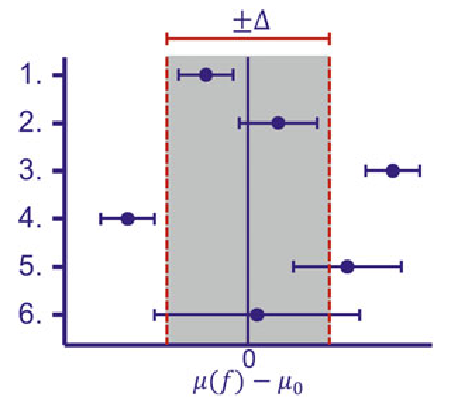
\includegraphics[
        width=\linewidth,
        height=5cm,
        keepaspectratio,
    ]{images/statistics/Equivalence-Testing.png}
    \caption*{
        Comparison between equivalence testing and traditional hypothesis testing.
        The vertical dotted lines represents the interval $[-\Delta, \Delta]$ and the vertical solid line represents the difference $\mu( f ) - \mu_0 = 0$. 
        The horizontal x-axis represents the difference $\mu( f ) - \mu_0$ and each dot in the figure represents an estimate of this difference. 
        The horizontal lines through the dots represent the $1 - 2\alpha$ confidence intervals.
        \cite{statistics/book/Statistics-for-Data-Scientists/Maurits-Kaptein}
    }
\end{figure}

    \item Equivalence testing $H_0 : \dabs{\mu( f ) - \mu_0} > \Delta$ against $H_a : \dabs{\mu( f ) - \mu_0} \leq \Delta$ is really different in concept from traditional hypothesis testing $H_0 : \mu( f ) = \mu_0$ against $H_a : \mu( f ) \neq \mu_0 $.
    \hfill \cite{statistics/book/Statistics-for-Data-Scientists/Maurits-Kaptein}
    \begin{enumerate}
        \item The $1 - 2\alpha$ confidence interval fall completely within $[-\Delta, \Delta]$, which means that the null hypothesis $H_0 : |\mu( f ) - \mu_0| > \Delta$ is being rejected. 
        It is not completely clear whether $H_0 : \mu( f ) = \mu_0$ is being rejected, since this can only be established if the $1 - \alpha$ confidence interval has been applied. 
        If we assume that this $1 - \alpha$ interval would fit within $[-\Delta, 0]$, the null hypothesis $H_0 : \mu( f ) = \mu_0$ would also be rejected. 
        This is a setting that we described earlier for large datasets, where the traditional hypothesis can be rejected for irrelevant differences.
        \hfill \cite{statistics/book/Statistics-for-Data-Scientists/Maurits-Kaptein}

        \item The null hypothesis $H_0 : |\mu( f ) - \mu_0| > \Delta$ for equivalence is being rejected, indicating that the population mean $\mu( f )$ is equivalent to $\mu_0 $. 
        The traditional hypothesis $H_0 : \mu( f ) = \mu_0$ is not being rejected, which implies that there is not enough evidence to believe that the population mean $\mu( f )$ is different from $\mu_0 $. 
        This means that both conclusions seem to coincide, although this does not imply that $\mu( f ) = \mu_0 $.
        \hfill \cite{statistics/book/Statistics-for-Data-Scientists/Maurits-Kaptein}

        \item The traditional null hypothesis is being rejected (assuming that the $95\%$ confidence interval would not contain zero) and equivalence cannot be claimed. 
        Thus both approaches seem to have similar conclusions: $\mu( f )$ is different and not equivalent to $\mu_0 $.
        \hfill \cite{statistics/book/Statistics-for-Data-Scientists/Maurits-Kaptein}

        \item This is the same as in the previous setting, although the results lie on the other side of the vertical line $\mu( f ) = \mu_0 $.
        \hfill \cite{statistics/book/Statistics-for-Data-Scientists/Maurits-Kaptein}

        \item The fact that one side of the confidence interval is contained in the interval $[-\Delta, \Delta]$ does not change the conclusions.
        \hfill \cite{statistics/book/Statistics-for-Data-Scientists/Maurits-Kaptein}

        \item Here we cannot demonstrate equivalence, but we cannot reject the traditional null hypothesis either. 
        Thus on the one hand there is not enough evidence to reject $\mu( f ) = \mu_0 $, but there is not enough evidence either to reject that $\dabs{\mu( f ) - \mu_0} > \Delta$.
        This seems contradictory, but it is probably an issue of a lack of information, since the $90\%$ confidence interval is too wide.
        \hfill \cite{statistics/book/Statistics-for-Data-Scientists/Maurits-Kaptein}
    \end{enumerate}

    \item The non-inferiority hypotheses look somewhat similar to the one-sided hypotheses, but they are not.
    In the traditional hypothesis testing format we would investigate the null hypothesis $H_0 : \mu_{N ew} \leq \mu_{Old}$ against $H_a : \mu_{N ew} > \mu_{Old}$ , assuming that a higher mean is a better clinical outcome.
    \hfill \cite{statistics/book/Statistics-for-Data-Scientists/Maurits-Kaptein}

    \item The collected data (typically through a randomized controlled clinical trial) would then have to demonstrate that the null hypothesis is rejected. 
    Thus the new treatment must demonstrate \textbf{superiority}. 
    \hfill \cite{statistics/book/Statistics-for-Data-Scientists/Maurits-Kaptein}

    \item Often new treatments are not (much) better in their clinical outcome, but they bring a secondary benefit. 
    For instance, the new treatment is much less invasive. 
    Superiority is then difficult to demonstrate. 
    Instead, we would like to show that the new treatment is not inferior to the old treatment. 
    Thus, the data must demonstrate that the new treatment is not too much worse than the old treatment: $H_a : \mu_{N ew} > \mu_{Old} - \Delta$, with $\Delta > 0$ the \textbf{non-inferiority margin}. 
    Thus, the null hypothesis becomes $H_0 : \mu_{N ew} \leq \mu_{Old} - \Delta$. 
    If this null hypothesis cannot be rejected, the new treatment is assumed inferior to the old treatment, since non-inferiority could not be proven.
    \hfill \cite{statistics/book/Statistics-for-Data-Scientists/Maurits-Kaptein}
\end{enumerate}





















\partition{Mathematics: Linear Algebra}
\chapter{Group Theory}




\section{Groups}

\begin{enumerate}
    \item \textbf{Definition}: Consider a set $\mathcal{G}$ and an (inner) operation $\otimes : \mathcal{G} \times \mathcal{G} \to \mathcal{G}$ group defined on $G$. Then $G := (\mathcal{G}, \otimes)$ is called a group if the following hold:
    \hfill \cite{mfml/book/mml/Deisenroth-Faisal-Ong}
    \begin{enumerate}
        \item Closure of $\mathcal{G}$ under $\otimes$: $\forall x, y \in \mathcal{G} : x \otimes y \in \mathcal{G}$
        \hfill \cite{mfml/book/mml/Deisenroth-Faisal-Ong}

        \item Associativity: $\forall x, y, z \in  \mathcal{G} : (x \otimes  y) \otimes  z = x \otimes  (y \otimes  z)$
        \hfill \cite{mfml/book/mml/Deisenroth-Faisal-Ong}

        \item Neutral element: $\exists e \in  \mathcal{G} \forall x \in  \mathcal{G} : x \otimes  e = x and e \otimes  x = x$
        \hfill \cite{mfml/book/mml/Deisenroth-Faisal-Ong}

        \item Inverse element: $\forall x \in  \mathcal{G} \exists y \in  \mathcal{G}$ : $x \otimes  y = e$ and $y \otimes  x = e$, where $e$ is the neutral element. We often write $x^{-1}$ to denote the inverse element of $x$.
        \hfill \cite{mfml/book/mml/Deisenroth-Faisal-Ong}
    \end{enumerate}

    \item The inverse element is defined with respect to the operation $\otimes$ and does not necessarily mean $\dfrac{1}{x}$.
    \hfill \cite{mfml/book/mml/Deisenroth-Faisal-Ong}

    \item Group allows only inner operation $\otimes$, means the operands \textbf{must be} elements from $\mathcal{G}$.

    \item Examples:
    \begin{enumerate}
        \item $(\mathbb{N}_0, +)$ is \textbf{not} a group: Although $(\mathbb{N}_0, +)$ possesses a neutral element ($0$), the inverse elements are missing.
        \hfill $\mathbb{N}_0 := \mathbb{N} \cup \dCurlyBrac{0}$
        \hfill \cite{mfml/book/mml/Deisenroth-Faisal-Ong}

        \item $(\mathbb{Z}, \cdot)$ is not a group: Although $(\mathbb{Z}, \cdot)$ contains a neutral element ($1$), the inverse elements for any $z \in \mathbb{Z}, z \neq \pm1$, are missing.
        \hfill \cite{mfml/book/mml/Deisenroth-Faisal-Ong}

        \item $(\mathbb{R}, \cdot)$ is not a group since $0$ does not possess an inverse element.
        \hfill \cite{mfml/book/mml/Deisenroth-Faisal-Ong}

        
    \end{enumerate}
\end{enumerate}






\section{Abelian Group}

\begin{enumerate}
    \item \textbf{Definition}: A group $G = (\mathcal{G}, \otimes)$ is called Abelian group if $\forall x, y \in \mathcal{G} : x \otimes y = y \otimes x$ (commutative)
    \hfill \cite{mfml/book/mml/Deisenroth-Faisal-Ong}

    \item Examples:
    \begin{enumerate}
        \item $(\mathbb{Z}, +)$ is an Abelian group
        \hfill \cite{mfml/book/mml/Deisenroth-Faisal-Ong}

        \item $( \mathbb{R} \backslash \dCurlyBrac{0}, \cdot)$ is Abelian
        \hfill \cite{mfml/book/mml/Deisenroth-Faisal-Ong}

        \item $(\mathbb{R}^n, +),(\mathbb{Z}^n, +), n \in \mathbb{N}$ are Abelian if + is defined component-wise:
        \\
        $
            (x_1, \cdots , x_n) + (y_1, \cdots , y_n) = (x_1 + y_1, \cdots , x_n + y_n)
        $
        \\
        Then, $(x_1, \cdots , x_n)^{-1} := (-x_1, \cdots , -x_n)$ is the inverse element and $e = (0, \cdots , 0)$ is the neutral element.

        \item $(\mathbb{R}^{m\times n} , +)$, the set of $m \times n$-matrices is Abelian  (with component-wise addition)

        
    \end{enumerate}
\end{enumerate}





\section{General Linear Group}

\begin{enumerate}
    \item \textbf{Definition}: The set of regular (invertible) matrices $A \in \mathbb{R}^{n\times n}$ is a group with respect to matrix multiplication and is called general linear group $GL(n, \mathbb{R})$. 
    
    \item However, since matrix multiplication is not commutative, the group is not Abelian.

    
\end{enumerate}


\chapter{Matrices}

\begin{enumerate}[itemsep=0.3cm]
    \item With $m, n \in \mathbb{N}$ a real-valued $(m, n)$ matrix $A$ is an $m\cdot n$-tuple of elements $a_{ij}$, $i = 1, \cdots , m$, $j = 1, \cdots , n$, which is ordered according to a rectangular scheme consisting of $m$ rows and $n$ columns:
    \\[0.2cm]
    $
        A
        = 
        \begin{bmatrix}
            a_{11} & a_{12} & \cdots & a_{1n} \\
            a_{21} & a_{22} & \cdots & a_{2n} \\
            \vdots & \vdots & \ddots & \vdots \\
            a_{m1} & a_{m2} & \cdots & a_{mn} \\
        \end{bmatrix}
        \hfill
        (\ a_{ij} \in \mathbb{R} \ )
    $
    \hfill \cite{mfml/book/mml/Deisenroth-Faisal-Ong}

    \item $\mathbb{R}^{m\times n}$ is the set of all real-valued $(m, n)$-matrices. $A \in \mathbb{R}^{m\times n}$ can be equivalently represented as $a \in \mathbb{R}^{mn}$ by stacking all $n$ columns of the matrix into a long vector.
    \hfill \cite{mfml/book/mml/Deisenroth-Faisal-Ong}

    \vspace{0.5cm}

    \item They can be used to compactly represent systems of linear equations, but they also represent linear functions (linear mappings).
    \hfill \cite{mfml/book/mml/Deisenroth-Faisal-Ong}
\end{enumerate}


\section{Matrix Operations}
\subsection{Matrix Addition ( $A+B$ ) \cite{mfml/book/mml/Deisenroth-Faisal-Ong}}

The sum of two matrices $A \in \mathbb{R}^{m\times n}$, $B \in \mathbb{R}^{m\times n}$ is defined as the element-wise sum:\\
. \hfill
\begin{customArrayStretch}{2}
$
    A + B
    := \begin{bmatrix}
        a_{11} + b_{11} &   \cdots  &  a_{1n} + b_{1n} \\
        \vdots          &   \ddots  &   \vdots  \\
        a_{m1} + b_{m1} &   \cdots  &  a_{mn} + b_{mn} \\
    \end{bmatrix}
    \in \mathbb{R}^{m\times n}
$
\end{customArrayStretch}
\hfill \cite{mfml/book/mml/Deisenroth-Faisal-Ong}







\begin{lstlisting}[
    language=Python,
    caption=Matrix Addition - numPy
]
import numpy as np

m,n = 4,3

A = np.random.randint(-10, 10, size=(m,n))
B = np.random.randint(-10, 10, size=(m,n))

C = A + B

print("A:\n", A)
print("B:\n", B)
print("C:\n", C)
\end{lstlisting}










\clearpage
\subsection{Matrix Multiplication ( $AB$ OR $@$ OR $\cdot$ ) \cite{mfml/book/mml/Deisenroth-Faisal-Ong}}

For matrices $\matname{A} \in \mathbb{R}^{m\times n}$, $\matname{B} \in \mathbb{R}^{n\times k}$, the elements $c_{ij}$ of the product matrices. $\matname{C} = \matname{AB} \in \mathbb{R}^{m\times k}$ are computed as:

\vspace{0.5cm}
\hfill
$
    c_{ij} = \dsum_{l=1}^n a_{il}\ b_{lj}
$
\hfill
$
    i = 1,\cdots,m
    \hspace{1cm}
    j = 1,\cdots,k
$
\hfill \cite{mfml/book/mml/Deisenroth-Faisal-Ong}





\begin{lstlisting}[
    language=Python,
    caption=Matrix Multiplication - numPy
]
import numpy as np

m,n,k = 4,3,5

A = np.random.randint(-10, 10, size=(m, n))
B = np.random.randint(-10, 10, size=(n, k))

C1 = A @ B
C2 = np.matmul(A, B)
C3 = np.dot(A, B)

print("A:\n", A)
print("B:\n", B)
print("C1:\n", C1)
print("C2:\n", C2)
print("C3:\n", C3)
print(np.all(C1 == C2), np.all(C1 == C3))
\end{lstlisting}




\vspace{0.5cm}

\begin{enumerate}
    \item To compute element $c_{ij}$ we multiply the elements of the $i$th row of $\matname{A}$ with the $j$th column of $\matname{B}$ and sum them up.
    \hfill \cite{mfml/book/mml/Deisenroth-Faisal-Ong}

    \item Matrices can only be multiplied if their “neighboring” dimensions match.
    \hfill \cite{mfml/book/mml/Deisenroth-Faisal-Ong}
    \\
    \hfill
    $
        \underset{n\times k}{\underbrace{\matname{A}}}\
        \underset{k\times m}{\underbrace{\matname{B}}}
        =
        \underset{n\times m}{\underbrace{\matname{C}}}
    $
    \hfill \cite{mfml/book/mml/Deisenroth-Faisal-Ong}
    \\
    The product $\matname{BA}$ is not defined if $m \neq n$ since the neighboring dimensions do not match.

    \item Matrix multiplication is \textbf{not} defined as an element-wise operation on matrix elements, i.e., 
    \\
    $c_{ij} \neq a_{ij}\ b_{ij}$ (even if the size of $\matname{A}$, $\matname{B}$ was chosen appropriately).
    \hfill \cite{mfml/book/mml/Deisenroth-Faisal-Ong}
\end{enumerate}


\subsubsection{Properties}

\begin{enumerate}
    \item matrix multiplication is \textbf{not} commutative: $\matname{AB} \neq \matname{BA}$
    \hfill \cite{mfml/book/mml/Deisenroth-Faisal-Ong}

    \item \textbf{Associativity}: 
    $
        \forall 
        \matname{A} \in \mathbb{R}^{m\times n},\ 
        \matname{B} \in \mathbb{R}^{n\times p},\ 
        \matname{C} \in \mathbb{R}^{p\times q}
    $:
    
        \begin{enumerate}
            \item $\matname{ABC} = (\matname{AB})\ \matname{C} = \matname{A}\ (\matname{BC})$
            \hfill \cite{mfml/book/mml/Deisenroth-Faisal-Ong}
        \end{enumerate}

    \item \textbf{Distributivity}: 
    $
        \forall 
        \matname{A},\ \matname{B}\in \mathbb{R}^{m\times n},\ 
        \matname{C},\ \matname{D}\in \mathbb{R}^{n\times p}
    $:

        \begin{enumerate}
            \item $(\matname{A} + \matname{B})\ \matname{C} = \matname{AC} + \matname{BC}$
            \hfill \cite{mfml/book/mml/Deisenroth-Faisal-Ong}
            
            \item $\matname{A}\ (\matname{C} + \matname{D}) = \matname{AC} + \matname{AD}$
            \hfill \cite{mfml/book/mml/Deisenroth-Faisal-Ong}
        \end{enumerate}

    \item Multiplication with the identity matrix: 
    $
        \forall 
        \matname{A},\ \matname{B}\in \mathbb{R}^{m\times n}
    $:
        \begin{enumerate}
            \item $\matname{I}_m\matname{A} = \matname{AI}_n = \matname{A}$
            \hfill $m\neq n \Rightarrow \matname{I}_m \neq \matname{I}_n$
            \hfill \cite{mfml/book/mml/Deisenroth-Faisal-Ong}
        \end{enumerate}
\end{enumerate}

















\clearpage
\subsection{Hadamard product ( $A \circ B$ OR $A \ast B$ ) \cite{mfml/book/mml/Deisenroth-Faisal-Ong}}

element-wise multiplication: For $A,B \in \mathbb{R}^{m\times n}$
\\
\ 
\hfill
$
    C = A \circ B \in \mathbb{R}^{m\times n}
$
\hfill
$
    c_{ij} = a_{ij}\ b_{ij}
$
\hfill
\ 













\begin{lstlisting}[
    language=Python,
    caption=Hadamard product - numPy
]
import numpy as np

m,n = 4,3

A = np.random.randint(-10, 10, size=(m,n))
B = np.random.randint(-10, 10, size=(m,n))

C = A * B

print("A:\n", A)
print("B:\n", B)
print("C:\n", C)
\end{lstlisting}












\clearpage
% \subsection{Matrix Inverse ( $A^{-1}$ ) \cite{mfml/book/mml/Deisenroth-Faisal-Ong}}
\subsection{Matrix Inverse \cite{mfml/book/mml/Deisenroth-Faisal-Ong}}

Consider a square matrix $\bm{A} \in \mathbb{R}^{n\times n}$. 
Let matrix $\bm{B} \in \mathbb{R}^{n\times n}$ have the property that $\bm{A}\bm{B} = \bm{I}_n = \bm{B}\bm{A}$. 
$\bm{B}$ is called the inverse of $\bm{A}$ and denoted by $\bm{A}^{-1}$.
\hfill \cite{mfml/book/mml/Deisenroth-Faisal-Ong}





\begin{lstlisting}[
    language=Python,
    caption=Matrix Inverse - numPy
]
import numpy as np

n = 4

A = np.random.randint(-10, 10, size=(n,n)).astype(float)
A_inv = np.linalg.inv(A)

print("A:\n", A)
print("A_inv:\n", A_inv)
print(A @ A_inv)
print(np.allclose((A @ A_inv) , np.eye(n, n)))
\end{lstlisting}






\begin{enumerate}
    \item \textbf{Not} every matrix $\bm{A}$ possesses an inverse $\bm{A}^{-1}$.
    \hfill \cite{mfml/book/mml/Deisenroth-Faisal-Ong}

    \item Only square matrices might have inverse. Non-square matrices \textbf{don't} have inverse.

    \item When the matrix inverse exists, it is \textbf{unique}.
    \hfill \cite{mfml/book/mml/Deisenroth-Faisal-Ong}

    \item $
        \bm{A} = \begin{bmatrix}
            a_{11} & a_{12} \\
            a_{21} & a_{22} \\
        \end{bmatrix} 
        \in \mathbb{R}^{2\times 2}
    $
    \hspace{1cm} and \hspace{1cm}
    $a_{11}\ a_{22} - a_{12}\ a_{21} \neq 0$ (determinant of $A$)\\[0.4cm] 
    $\Rightarrow$
    $
        \bm{A}^{-1} = 
        \dfrac{1}{a_{11}\ a_{22} - a_{12}\ a_{21}}
        \begin{bmatrix}
            a_{22} & -a_{12} \\
            -a_{21} & a_{11} \\
        \end{bmatrix}
    $
    \hfill \cite{mfml/book/mml/Deisenroth-Faisal-Ong}

\end{enumerate}



\subsubsection{Matrix Inverse using Gaussian Elimination}

\begin{enumerate}
    \item Given a matrix $\bm{A} \in \mathbb{R}^{n\times n}$, we need to find $\bm{X} = \bm{A}^{-1}$ such that $\bm{A}\bm{X} = \bm{I}_n$
    \hfill \cite{mfml/book/mml/Deisenroth-Faisal-Ong}
    
    \item We can write this down as a set of simultaneous linear equations $\bm{A}\bm{X} = \bm{I}_n$, where we solve for $\bm{X} = [\bm{x}_1| \cdots |\bm{x}_n]$. 
    \hfill \cite{mfml/book/mml/Deisenroth-Faisal-Ong}

    \item augmented matrix notation for a compact representation of this set of systems of linear equations:
    \hfill \cite{mfml/book/mml/Deisenroth-Faisal-Ong}
    \\
    .\hfill
    $
        [\bm{A}|\bm{I}_n] 
        \curlyrightarrow \cdots \curlyrightarrow 
        [\bm{I}_n|\bm{A}^{-1}]
    $
    \hfill \cite{mfml/book/mml/Deisenroth-Faisal-Ong}

    
\end{enumerate}




\subsubsection{Moore-Penrose pseudo-inverse}

$
    \begin{aligned}
                         & \bm{A}\bm{X} = \bm{I} \\
        \Leftrightarrow\ & \bm{A}^\top \bm{A}\bm{X} = \bm{A}^\top \\
        \Leftrightarrow\ & \bm{X} = (\bm{A}^\top \bm{A})^{-1} \bm{A}^\top \\
    \end{aligned}
$
\hfill \cite{mfml/book/mml/Deisenroth-Faisal-Ong}


\vspace{0.2cm}

\begin{enumerate}
    \item Disadvantages:
    \begin{enumerate}
        \item requires many computations for the matrix-matrix product and computing the inverse of $\bm{A}^\top \bm{A}$. 
        \hfill \cite{mfml/book/mml/Deisenroth-Faisal-Ong}

        \item for reasons of numerical precision it is generally not recommended
        \hfill \cite{mfml/book/mml/Deisenroth-Faisal-Ong}
    \end{enumerate}
\end{enumerate}





\subsubsection{Properties}

\begin{multicols}{2}
\begin{enumerate}
    \item $\bm{A}\bm{A}^{-1} = \bm{I} = \bm{A}^{-1}\bm{A}$
    \hfill \cite{mfml/book/mml/Deisenroth-Faisal-Ong}

    \item $(\bm{A}\bm{B})^{-1} = \bm{B}^{-1}\ \bm{A}^{-1}$
    \hfill \cite{mfml/book/mml/Deisenroth-Faisal-Ong}

    \item $(\bm{A} + \bm{B})^{-1} \neq \bm{A}^{-1} + \bm{B}^{-1}$
    \hfill \cite{mfml/book/mml/Deisenroth-Faisal-Ong}

    \item $(\bm{A}^{-1})^\top = (\bm{A}^\top)^{-1} =: \bm{A}^{-\top}$
    \hfill \cite{mfml/book/mml/Deisenroth-Faisal-Ong}

    \item $(\bm{A}^{-1})^{-1} =  \bm{A}$
    
\end{enumerate}
\end{multicols}
















\clearpage
\section{Types of matrices}
\subsection{Identity Matrix ( $I_n$ )}

In $\mbbR^{n\times n}$, we define the identity matrix:\\
\vspace{0.5cm}
\hfill
$
    \bm{I}_n
    := \begin{bmatrix}
        1 & 0 & \cdots & 0 & \cdots & 0 \\
        0 & 1 & \cdots & 0 & \cdots & 0 \\
        \vdots & \vdots & \ddots & \vdots & \ddots & \vdots \\
        0 & 0 & \cdots & 1 & \cdots & 0 \\
        \vdots & \vdots & \ddots & \vdots & \ddots & \vdots \\
        0 & 0 & \cdots & 0 & \cdots & 1 \\
    \end{bmatrix}
    \in \mbbR^{n\times n}
$
\hfill \cite{mfml/book/mml/Deisenroth-Faisal-Ong}
\\
as the $n \times n$-matrix containing $1$ on the diagonal and $0$ everywhere else.







\begin{lstlisting}[
    language=Python,
    caption=Identity Matrix - numPy
]
import numpy as np

n = 4

print(np.eye(n,n))
\end{lstlisting}









\subsection{regular/invertible/non-singular matrix}

A matrix $A$ is called regular/invertible/non-singular if $A^{-1}$ exists.






\subsection{singular/non-invertible matrix}

A matrix $A$ is called singular/non-invertible if $A^{-1}$ \textbf{doesn't} exists.













\chapter{Vector Spaces}


\section{Vector Space}

\begin{enumerate}
    \item \textbf{Definition}: A real-valued vector space $V = (\mathcal{V}, +, \cdot)$ is a set $\mathcal{V}$ with two operations:
    \hfill \cite{mfml/book/mml/Deisenroth-Faisal-Ong}
    \begin{enumerate}
        \item[] $+ :  \mathcal{V} \times \mathcal{V} \to \mathcal{V}$
        \hfill \cite{mfml/book/mml/Deisenroth-Faisal-Ong}

        \item[] $\cdot: \mathbb{R} \times \mathcal{V} \to \mathcal{V}$ 
        \hfill \cite{mfml/book/mml/Deisenroth-Faisal-Ong}
    \end{enumerate}


    \item addition ($+$) is inner operation: both operands must be from $\mathcal{V}$
    \hfill \cite{mfml/book/mml/Deisenroth-Faisal-Ong}

    \item multiplication by scalars ($\cdot$) is outer operation: one operand is from $\mathcal{V}$, another from $\mathbb{R}$
    \hfill \cite{mfml/book/mml/Deisenroth-Faisal-Ong}

    \item The elements $\bm{x} \in \mathcal{V}$ are called \textbf{vectors}.
    \hfill \cite{mfml/book/mml/Deisenroth-Faisal-Ong}
\end{enumerate}


\subsection{Properties of a vector Space}

\begin{enumerate}
    \item $(\mathcal{V}, +)$ is an Abelian group
    \hfill \cite{mfml/book/mml/Deisenroth-Faisal-Ong}

    \item Distributivity:
    \begin{enumerate}
        \item $\forall \lambda  \in  \mathbb{R}, \bm{x}, \bm{y} \in  \mathcal{V} : \lambda  \cdot  (\bm{x} + \bm{y}) = \lambda  \cdot  \bm{x} + \lambda  \cdot  \bm{y}$
        \hfill \cite{mfml/book/mml/Deisenroth-Faisal-Ong}

        \item $\forall \lambda , \psi  \in  \mathbb{R}, \bm{x} \in  \mathcal{V} : (\lambda  + \psi ) \cdot  \bm{x} = \lambda  \cdot  \bm{x} + \psi  \cdot  \bm{x}$
        \hfill \cite{mfml/book/mml/Deisenroth-Faisal-Ong}
    \end{enumerate}

    \item Associativity (outer operation): $\forall \lambda , \psi  \in  \mathbb{R}, \bm{x} \in  \mathcal{V} : \lambda \cdot (\psi \cdot x) = (\lambda \psi )\cdot \bm{x}$
    \hfill \cite{mfml/book/mml/Deisenroth-Faisal-Ong}

    \item Neutral element with respect to the outer operation: $\forall \bm{x} \in  \mathcal{V} : 1\cdot \bm{x} = \bm{x}$
    \hfill \cite{mfml/book/mml/Deisenroth-Faisal-Ong}

    \item The neutral element of $(\mathcal{V}, +)$ is the zero vector $\bm{0} = [0, \cdots , 0]^\top$
    \hfill \cite{mfml/book/mml/Deisenroth-Faisal-Ong}

    \item A “vector multiplication” $\bm{ab}, \bm{a}, \bm{b} \in \mathbb{R}^n$, is \textbf{not defined}.
    \hfill \cite{mfml/book/mml/Deisenroth-Faisal-Ong}
\end{enumerate}


\subsection{Dimension of a vector Space}


\begin{enumerate}
    \item the dimension of $V$ is the number of basis vectors of $V$ , and we write $\dim(V)$.
    \hfill \cite{mfml/book/mml/Deisenroth-Faisal-Ong}

    \item The dimension of a vector space corresponds to the number of its basis vectors.
    \hfill \cite{mfml/book/mml/Deisenroth-Faisal-Ong}

    \item Intuitively, the dimension of a vector space can be thought of as the number of independent directions in this vector space.
    \hfill \cite{mfml/book/mml/Deisenroth-Faisal-Ong}

    \item The dimension of a vector space is not necessarily the number of elements in a vector. 
    For instance, the vector space $V = \text{span}[\begin{bmatrix}0 \\ 1\end{bmatrix}]$ is one-dimensional, although the basis vector possesses two elements.
    \hfill \cite{mfml/book/mml/Deisenroth-Faisal-Ong}
\end{enumerate}


\subsection{Norm}

\begin{enumerate}
    \item \textbf{Definition}: A norm on a vector space $V$ is a function
    \hfill \cite{mfml/book/mml/Deisenroth-Faisal-Ong}
    \\
    .\hfill
    $\dnorm{\cdot}: V \to \mathbb{R}$ such that $\bm{x} \mapsto \dnorm{\bm{x}}$
    \hfill \cite{mfml/book/mml/Deisenroth-Faisal-Ong}
    \\
    which assigns each vector $\bm{x}$ its length $\dnorm{\bm{x}} \in \mathbb{R}$, such that for all $\lambda \in \mathbb{R}$ and $\bm{x}, \bm{y} \in V$ the following hold:
    \hfill \cite{mfml/book/mml/Deisenroth-Faisal-Ong}
    \begin{enumerate}
        \item Absolutely homogeneous: $\dnorm{\lambda \bm{x}} = \dabs{\lambda} \dnorm{\bm{x}}$
        \hfill \cite{mfml/book/mml/Deisenroth-Faisal-Ong}

        \item Triangle inequality: $\dnorm{\bm{x} + \bm{y}} \leq \dnorm{\bm{x}} + \dnorm{\bm{y}}$
        \hfill \cite{mfml/book/mml/Deisenroth-Faisal-Ong}
        \\
        In geometric terms, the triangle inequality states that for any triangle, the sum of the lengths of any two sides must be greater than or equal to the length of the remaining side.
        

        \item Positive definite: $\dnorm{\bm{x}} \geq 0$ and $\dnorm{\bm{x}} = 0 \Leftrightarrow \bm{x} = \bm{0}$
        \hfill \cite{mfml/book/mml/Deisenroth-Faisal-Ong}
    \end{enumerate}
\end{enumerate}




\subsection{Inner Product Space}

\begin{enumerate}
    \item Let $V$ be a vector space and $\Omega  : V \times  V \to  \mathbb{R}$ be a bilinear mapping that takes two vectors and maps them onto a real number. 
    Then the pair $(V, \dAngleBrac{\cdot, \cdot})$ is called an \textbf{inner product space} or \textbf{(real) vector space with inner product}.
\end{enumerate}




\subsection{Euclidean vector space}

\begin{enumerate}
    \item Let $V$ be a vector space and $\Omega : V \times V \to \mathbb{R}$ be a bilinear mapping that takes two vectors and maps them onto a real number. Then if we use the dot product, we call $(V,\dAngleBrac{\cdot, \cdot})$ a Euclidean vector space.
\end{enumerate}



\subsection{Lengths}

\begin{enumerate}
    \item Inner products and norms are closely related in the sense that any inner product induces a norm
    \hfill \cite{mfml/book/mml/Deisenroth-Faisal-Ong}
    \\
    .\hfill
    $\dnorm{\bm{x}} := \sqrt{\dAngleBrac{\bm{x}, \bm{x}}}$
    \hfill \cite{mfml/book/mml/Deisenroth-Faisal-Ong}
    \\
    in a natural way, such that we can compute lengths of vectors using the inner product.
    \hfill \cite{mfml/book/mml/Deisenroth-Faisal-Ong}

    \item length = norm
    \hfill \cite{common/online/chatgpt}
    \\
    different norms lead to different lengths
    \hfill \cite{common/online/chatgpt}

    \item Not every norm is induced by an inner product (eg: Manhattan norm).
    \hfill \cite{mfml/book/mml/Deisenroth-Faisal-Ong}

    \item \textbf{Cauchy-Schwarz Inequality}: For an inner product vector space $(V,\dAngleBrac{\cdot, \cdot})$ the induced norm $\dnorm{\cdot}$ satisfies the Cauchy-Schwarz inequality
    \hfill \cite{mfml/book/mml/Deisenroth-Faisal-Ong}
    \\
    .\hfill
    $\dabs{\dAngleBrac{\bm{x}, \bm{y}}} \leq \dnorm{\bm{x}} \dnorm{\bm{y}}$
    \hfill \cite{mfml/book/mml/Deisenroth-Faisal-Ong}

    \item Transformations by orthogonal matrices are special because the length of a vector $\bm{x}$ is not changed when transforming it using an orthogonal matrix $\bm{A}$. 
    For the dot product, we obtain
    \hfill \cite{mfml/book/mml/Deisenroth-Faisal-Ong}
    \\
    .\hfill
    $
        \dnorm{\bm{Ax}}^2 
        = (\bm{Ax})^\top (\bm{Ax})
        = \bm{x}^\top \bm{A}^\top \bm{Ax}
        = \bm{x}^\top \bm{Ix}
        = \bm{x}^\top \bm{x}
        = \dnorm{\bm{x}}^2
    $
    \hfill \cite{mfml/book/mml/Deisenroth-Faisal-Ong}
\end{enumerate}





\subsection{Distance}

\begin{enumerate}
    \item Consider an inner product space $(V,\dAngleBrac{\cdot, \cdot})$. 
    Then
    \hfill \cite{mfml/book/mml/Deisenroth-Faisal-Ong}
    \\
    .\hfill
    $
        d(\bm{x}, \bm{y})
        := \dnorm{\bm{x} - \bm{y}}
        = \sqrt{\dAngleBrac{\bm{x} - \bm{y}, \bm{x} - \bm{y}}}
    $
    \hfill \cite{mfml/book/mml/Deisenroth-Faisal-Ong}
    \\
    is called the distance between $\bm{x}$ and $\bm{y}$ for $\bm{x}, \bm{y} \in V$ .
    \hfill \cite{mfml/book/mml/Deisenroth-Faisal-Ong}

    \item If we use the dot product as the inner product, then the distance is called \textbf{Euclidean distance}.
    \hfill \cite{mfml/book/mml/Deisenroth-Faisal-Ong}

    \item Similar to the length of a vector, the distance between vectors does not require an inner product: a norm is sufficient.
    If we have a norm induced by an inner product, the distance may vary depending on the choice of the inner product. 
    \hfill \cite{mfml/book/mml/Deisenroth-Faisal-Ong}

    \item Every distance is a metric, but not every metric is necessarily defined as a distance using a norm or inner product.
    \hfill \cite{common/online/chatgpt}

    \item \item Transformations with orthogonal matrices preserve distances.
    \hfill \cite{mfml/book/mml/Deisenroth-Faisal-Ong}
\end{enumerate}




\subsection{Metric}

\begin{enumerate}
    \item \textbf{Definition}: The mapping $d : V \times V \to \mathbb{R}$, $(\bm{x}, \bm{y}) \mapsto d(\bm{x}, \bm{y})$ is called a \textbf{metric}.
    \hfill \cite{mfml/book/mml/Deisenroth-Faisal-Ong}

    \item A metric $d$ satisfies the following:
    \hfill \cite{mfml/book/mml/Deisenroth-Faisal-Ong}
    \begin{enumerate}
        \item $d$ is \textbf{positive definite}, i.e., $d(\bm{x}, \bm{y}) \geq 0$ for all $\bm{x}, \bm{y} \in V$ and $d(\bm{x}, \bm{y}) = 0 \Leftrightarrow \bm{x} = \bm{y}$ .
        \hfill \cite{mfml/book/mml/Deisenroth-Faisal-Ong}

        \item $d$ is \textbf{symmetric}, i.e., $d(\bm{x}, \bm{y}) = d(\bm{y}, \bm{x})$ for all $\bm{x}, \bm{y} \in V$ .
        \hfill \cite{mfml/book/mml/Deisenroth-Faisal-Ong}

        \item \textbf{Triangle inequality}: $d(\bm{x}, \bm{z}) \leq d(\bm{x}, \bm{y}) + d(\bm{y}, \bm{z})$ for all $\bm{x}, \bm{y}, \bm{z} \in V$ .
        \hfill \cite{mfml/book/mml/Deisenroth-Faisal-Ong}
    \end{enumerate}
\end{enumerate}



\subsection{Inner Product VS Metric}

\begin{enumerate}
    \item the lists of properties of inner products and metrics look very similar. 
    \hfill \cite{mfml/book/mml/Deisenroth-Faisal-Ong}

    \item $\dAngleBrac{\bm{x}, \bm{y}}$ and $d(\bm{x}, \bm{y})$ behave in opposite directions.
    \hfill \cite{mfml/book/mml/Deisenroth-Faisal-Ong}

    \item Very similar $\bm{x}$ and $\bm{y}$ will result in a large value for the inner product and a small value for the metric.
    \hfill \cite{mfml/book/mml/Deisenroth-Faisal-Ong}
\end{enumerate}




\subsection{Angles}

\begin{enumerate}
    \item We use the Cauchy-Schwarz inequality to define angles $\omega$ in inner product spaces between two vectors $\bm{x}, \bm{y}$, and this notion coincides with our intuition in $\mathbb{R}^2$ and $\mathbb{R}^3$. 
    Assume that $\bm{x} \neq \bm{0}$, $\bm{y} \neq \bm{0}$. 
    Then
    $
        -1 \leq \dfrac{\dAngleBrac{\bm{x}, \bm{y}}}{\dnorm{\bm{x}} \dnorm{\bm{y}}} \leq 1
    $. 
    Therefore, there exists a unique $\omega \in [0, \pi]$ with 
    $
        \cos(\omega) = \dfrac{\dAngleBrac{\bm{x}, \bm{y}}}{\dnorm{\bm{x}} \dnorm{\bm{y}}}
    $
    \hfill \cite{mfml/book/mml/Deisenroth-Faisal-Ong}

    \item The number $\omega$ is the angle between the vectors $\bm{x}$ and $\bm{y}$.
    \hfill \cite{mfml/book/mml/Deisenroth-Faisal-Ong}

    \item Intuitively, the angle between two vectors tells us how similar their orientations are.
    \hfill \cite{mfml/book/mml/Deisenroth-Faisal-Ong}

    \item Transformations with orthogonal matrices preserve angles.
    \hfill \cite{mfml/book/mml/Deisenroth-Faisal-Ong}
    \\
    The angle between any two vectors $\bm{x}, \bm{y}$, as measured by their inner product, is also unchanged when transforming both of them using an orthogonal matrix $\bm{A}$. 
    Assuming the dot product as the inner product, the angle of the images $\bm{Ax}$ and $\bm{Ay}$ is given as
    \hfill \cite{mfml/book/mml/Deisenroth-Faisal-Ong}
    \\
    .\hfill
    $
        \cos \omega
        = \dfrac{(\bm{Ax})^\top (\bm{Ax})}{\dnorm{\bm{Ax}} \dnorm{\bm{Ax}}}
        = \dfrac{\bm{x}^\top \bm{A}^\top\bm{Ay}}{\sqrt{\bm{x}^\top \bm{A}^\top\bm{Ax} \bm{y}^\top \bm{A}^\top\bm{Ay}}}
        = \dfrac{\bm{x}^\top \bm{y}}{\dnorm{\bm{x}} \dnorm{\bm{y}}}
    $
    \hfill \cite{mfml/book/mml/Deisenroth-Faisal-Ong}
    \\
    which gives exactly the angle between $\bm{x}$ and $\bm{y}$.
\end{enumerate}

\begin{customArrayStretch}{1.3}
\begin{table}[H]
    \centering
    \begin{tabular}{|l|l|l|}
        \hline
        $\omega$ & $\cos(\omega)$ & Interpretation \\
        \hline
        $0$ & $1$ & orientation is same \\
        ${\pi}/{2}$ & $0$ & perpendicular \\
        $\pi$ & $-1$ & opposite direction \\
        \hline
    \end{tabular}
\end{table}
\end{customArrayStretch}




















\section{Vector Subspace/ linear subspace}


\begin{enumerate}
    \item \textbf{Definition}: Let $V = (\mathcal{V}, +, \cdot )$ be a vector space and $\mathcal{U} \subseteq \mathcal{V}, \mathcal{U} \neq \phi$. 
    Then $U = (\mathcal{U}, +, \cdot )$ is called vector subspace of $V$ (or linear subspace) if $U$ is a vector space with the vector space operations $+$ and $\cdot$  restricted to $\mathcal{U} \times \mathcal{U}$ and $\mathbb{R} \times \mathcal{U}$. 
    We write $U \subseteq V$ to denote a subspace $U$ of $V$.
    \hfill \cite{mfml/book/mml/Deisenroth-Faisal-Ong}

    \item Intuitively, they are sets contained in the original vector space with the property that when we perform vector space operations on elements within this subspace, we will never leave it. 
    In this sense, they are “closed”.
    \hfill \cite{mfml/book/mml/Deisenroth-Faisal-Ong}

    \item If $\mathcal{U} \subseteq \mathcal{V}$ and $V$ is a vector space, then $U$ naturally inherits many properties directly from $V$ because they hold for all $\bm{x} \in \mathcal{V}$, and in particular for all $\bm{x} \in \mathcal{U} \subseteq \mathcal{V}$. 
    This includes the Abelian group properties, the distributivity, the associativity and the neutral element.
    \hfill \cite{mfml/book/mml/Deisenroth-Faisal-Ong}

    \item To determine whether $(\mathcal{U}, +, \cdot)$ is a subspace of V we still do need to show:
    \begin{enumerate}
        \item $\mathcal{U} \neq \phi$, in particular: $\bm{0} \in \mathcal{U}$
        \hfill \cite{mfml/book/mml/Deisenroth-Faisal-Ong}

        \item Closure of $U$:
        \begin{enumerate}
            \item With respect to the outer operation: $\forall \lambda  \in  \mathbb{R} \forall \bm{x} \in  \mathcal{U} : \lambda \bm{x} \in  \mathcal{U}$.
            \hfill \cite{mfml/book/mml/Deisenroth-Faisal-Ong}
            
            \item With respect to the inner operation: $\forall \bm{x}, \bm{y} \in  \mathcal{U} : \bm{x} + \bm{y} \in  \mathcal{U}$.
            \hfill \cite{mfml/book/mml/Deisenroth-Faisal-Ong}
        \end{enumerate}
    \end{enumerate}

\end{enumerate}


\subsection{Dimension of a Vector Subspace}

\begin{enumerate}
    \item If $U \subseteq V$ is a subspace of $V$ , then $\dim(U) \leq \dim(V )$ and $\dim(U) = \dim(V )$ if and only if $U = V$ .
    \hfill \cite{mfml/book/mml/Deisenroth-Faisal-Ong}
\end{enumerate}



\subsection{Basis of a Vector Subspace}

\begin{enumerate}
    \item A basis of a subspace $U = \text{span}[\bm{x}_1, \cdots , \bm{x}_m] \subseteq \mathbb{R}^n$ can be found by executing the following steps:
    \hfill \cite{mfml/book/mml/Deisenroth-Faisal-Ong}
    \begin{enumerate}
        \item Write the spanning vectors as columns of a matrix $\bm{A}$
        \hfill \cite{mfml/book/mml/Deisenroth-Faisal-Ong}

        \item Determine the row-echelon form (REF) of $\bm{A}$.
        \hfill \cite{mfml/book/mml/Deisenroth-Faisal-Ong}

        \item The spanning vectors associated with the pivot columns are a basis of $U$.
        \hfill \cite{mfml/book/mml/Deisenroth-Faisal-Ong}
    \end{enumerate}
\end{enumerate}
























\section{Vector}

\begin{enumerate}
    \item In general, vectors are special objects that can be added together and multiplied by scalars to produce another object of the same kind. From an abstract mathematical viewpoint, any object that satisfies these two properties can be considered a vector. 
    \hfill \cite{mfml/book/mml/Deisenroth-Faisal-Ong}

    \item By convention $(1, n)$-matrices are called rows and $(m, 1)$-matrices are called row columns. 
    These special matrices are also called row/ column vectors.
    \hfill \cite{mfml/book/mml/Deisenroth-Faisal-Ong}

    \item Geometric vectors directed line segments that start at the origin, then intuitively the length of a vector is the distance of the “end” of this directed line segment from the origin.
    \hfill \cite{mfml/book/mml/Deisenroth-Faisal-Ong}
\end{enumerate}




\subsection{Types of vectors}

\begin{enumerate}
    \item $\mathbb{R}^n$ or $\mathbb{R}^{n\times 1}$ : column vectors: 
    $
        \bm{x} = 
        \begin{bmatrix}
            x_1\\ \vdots \\ x_n
        \end{bmatrix}
    $
    \hfill \cite{mfml/book/mml/Deisenroth-Faisal-Ong}

    \item $\mathbb{R}^{1\times n}$ : row vectors: 
    $
        \bm{x}^\top = \begin{bmatrix}x_1 & \cdots & x_n\end{bmatrix}
    $
    \hfill \cite{mfml/book/mml/Deisenroth-Faisal-Ong}
\end{enumerate}






\subsection{Manhattan Norm/ $\ell_1$ Norm}

\begin{enumerate}
    \item The Manhattan norm on $\mathbb{R}^n$ is defined for $\bm{x} \in \mathbb{R}^n$ as
    \hfill \cite{mfml/book/mml/Deisenroth-Faisal-Ong}
    \\
    .\hfill
    $
        \dnorm{\bm{x}}_1 := \dsum^n_{i=1} \dabs{x_i}
    $
    \hfill \cite{mfml/book/mml/Deisenroth-Faisal-Ong}
    \\
    where $\dabs{\cdot}$ is the absolute value.
    \hfill \cite{mfml/book/mml/Deisenroth-Faisal-Ong}
\end{enumerate}



\subsection{Euclidean Norm/ $\ell_2$ Norm}

\begin{enumerate}
    \item The Euclidean norm of $\bm{x} \in \mathbb{R}^n$ is defined as
    \hfill \cite{mfml/book/mml/Deisenroth-Faisal-Ong}
    \\
    .\hfill
    $
        \dnorm{\bm{x}}_2 := \sqrt{ \dsum^n_{i=1} x_i^2 } = \sqrt{\bm{x}^\top\bm{x}}
    $
    \hfill \cite{mfml/book/mml/Deisenroth-Faisal-Ong}
    \\
    and computes the Euclidean distance of $\bm{x}$ from the origin.
    \hfill \cite{mfml/book/mml/Deisenroth-Faisal-Ong}

    \item default "norm", if not stated otherwise.
    \hfill \cite{mfml/book/mml/Deisenroth-Faisal-Ong}
\end{enumerate}



\subsection{Outer Product ($ab^\top$) }

\begin{enumerate}
    \item $\forall \bm{a}, \bm{b} \in \mathbb{R}^n, \bm{ab}^\top \in \mathbb{R}^{n\times n}$
    \hfill \cite{mfml/book/mml/Deisenroth-Faisal-Ong}
    
\end{enumerate}



\subsection{General Inner Product ( $\Omega(a, b)$ )}

\begin{enumerate}
    \item A bilinear mapping $\Omega$ is a mapping with two arguments, and it is linear in each argument, i.e., when we look at a vector space $V$ then it holds that for all $\bm{x}, \bm{y}, \bm{z} \in V, \lambda , \psi  \in \mathbb{R}$ that
    \hfill \cite{mfml/book/mml/Deisenroth-Faisal-Ong}
    \\
    .\hfill
    $\Omega(\lambda \bm{x} + \psi \bm{y}, \bm{z}) = \lambda \Omega(\bm{x}, \bm{z}) + \psi \Omega(\bm{y}, \bm{z})$
    \hfill \cite{mfml/book/mml/Deisenroth-Faisal-Ong}
    \\
    .\hfill
    $\Omega(\bm{x}, \lambda \bm{y} + \psi \bm{z}) = \lambda \Omega(\bm{x}, \bm{y}) + \psi \Omega(\bm{x}, \bm{z})$.
    \hfill \cite{mfml/book/mml/Deisenroth-Faisal-Ong}

    \item Let $V$ be a vector space and $\Omega : V \times  V \to \mathbb{R}$ be a bilinear mapping that takes two vectors and maps them onto a real number. Then
    \hfill \cite{mfml/book/mml/Deisenroth-Faisal-Ong}
    \begin{enumerate}
        \item $\Omega$ is called \textbf{symmetric} if $\Omega(\bm{x}, \bm{y}) = \Omega(\bm{y}, \bm{x})$ for all $\bm{x}, \bm{y} \in  V$ , i.e., the order of the arguments does not matter.
        \hfill \cite{mfml/book/mml/Deisenroth-Faisal-Ong}

        \item $\Omega$ is called \textbf{positive definite} if $\forall \bm{x} \in  V \backslash \dCurlyBrac{\bm{0}} : \Omega(\bm{x}, \bm{x}) > 0 , \Omega(\bm{0}, \bm{0}) = 0$.
        \hfill \cite{mfml/book/mml/Deisenroth-Faisal-Ong}
    \end{enumerate}

\end{enumerate}





\subsection{Inner Product ( $<x, y>$ )}

\begin{enumerate}
    \item Let $V$ be a vector space and $\Omega  : V \times  V \to  \mathbb{R}$ be a bilinear mapping that takes two vectors and maps them onto a real number. Then
    \begin{enumerate}
        \item A positive definite, symmetric bilinear mapping $\Omega  : V \times  V \to  \mathbb{R}$ is called an inner product on $V$ . 
        We typically write $\dAngleBrac{x, y}$ instead of $\Omega (x, y)$.        
    \end{enumerate}
\end{enumerate}





\subsection{Scalar/dot product ($a^\top b$)}


\begin{enumerate}
    \item $
        \forall \bm{a}, \bm{b} \in \mathbb{R}^n, 
        \bm{a}^\top \bm{b} = \dsum^n_{i=1} a_i b_i \in \mathbb{R}    
    $
    \hfill \cite{mfml/book/mml/Deisenroth-Faisal-Ong}
    
\end{enumerate}



\subsection{Orthogonal ( $x \perp y$ ) \& orthonormal vectors}

\begin{enumerate}
    \item \textbf{Definition}: Two vectors $\bm{x}$ and $\bm{y}$ are orthogonal if and only if $\dAngleBrac{\bm{x}, \bm{y}} = 0$, and we write $\bm{x} \perp \bm{y}$. 
    \hfill \cite{mfml/book/mml/Deisenroth-Faisal-Ong}
    
    \item If additionally $\dnorm{\bm{x}} = 1 = \dnorm{\bm{y}}$, i.e., the vectors are unit vectors, then $\bm{x}$ and $\bm{y}$ are orthonormal.
    \hfill \cite{mfml/book/mml/Deisenroth-Faisal-Ong}

    \item $\bm{0}$-vector is orthogonal to every vector in the vector space.
    \hfill \cite{mfml/book/mml/Deisenroth-Faisal-Ong}

    \item Orthogonality is the generalization of the concept of perpendicularity to bilinear forms that do not have to be the dot product.
    \hfill \cite{mfml/book/mml/Deisenroth-Faisal-Ong}
\end{enumerate}



























\section{Linear Combination}

\begin{enumerate}
    \item \textbf{Definition}: Consider a vector space $V$ and a finite number of vectors $\bm{x}_1, \cdots , \bm{x}_k \in V$ . 
    Then, every $\bm{v} \in V$ of the form:
    \\
    .\hfill
    $
        \bm{v} 
        = \lambda _1 \bm{x}_1 + \cdots + \lambda _k \bm{x}_k
        = \dsum_{i=1}^k \lambda _i \bm{x}_i
        \in V
    $
    \hfill.
    \\
    with $\lambda _1, \cdots , \lambda _k \in \mathbb{R}$ is a linear combination of the vectors $\bm{x}_1, \cdots , \bm{x}_k$.
    \hfill \cite{mfml/book/mml/Deisenroth-Faisal-Ong}

    \item The $\bm{0}$-vector can always be written as the linear combination of $k$ vectors $\bm{x}_1, \cdots , \bm{x}_k$ because $\bm{0} = \dsum ^k _{i=1} 0 \bm{x}_i$ is always true.
    \hfill \cite{mfml/book/mml/Deisenroth-Faisal-Ong}

    
\end{enumerate}







\section{Affine Subspaces}

\begin{enumerate}
    \item \textbf{Definition}: Let $V$ be a vector space, $\bm{x}_0 \in V$ and $U \subseteq V$ a subspace. 
    Then the subset 
    \hfill \cite{mfml/book/mml/Deisenroth-Faisal-Ong}
    \\
    .\hfill
    $
        L 
        = \bm{x}_0 + U 
        := \dCurlyBrac{\bm{x}_0 + \bm{u} : \bm{u} \in  U}
        = \dCurlyBrac{\bm{v} \in  V | \exists \bm{u} \in  U : \bm{v} = \bm{x}_0 + \bm{u}} \subseteq V
    $
    \hfill \cite{mfml/book/mml/Deisenroth-Faisal-Ong}
    \\
    is called \textbf{affine subspace} or \textbf{linear manifold} of $V$.
    $U$ is called \textbf{direction} or \textbf{direction space}, and $\bm{x}_0$ is called \textbf{support point}.
    $L$ is also known as \textbf{hyperplane}.
    \hfill \cite{mfml/book/mml/Deisenroth-Faisal-Ong}

    \item Note that the definition of an affine subspace excludes $\bm{0}$ if $\bm{x}_0 \notin U$.
    Therefore, an affine subspace is not a (linear) subspace (vector subspace) of $V$ for $\bm{x}_0 \notin U$.
    \hfill \cite{mfml/book/mml/Deisenroth-Faisal-Ong}

    \item Consider two affine subspaces $L = \bm{x}_0 + U$ and $\tilde{L} = \tilde{\bm{x}}_0 + \tilde{U}$ of a vector space $V$ . 
    Then, $L \subseteq \tilde{L}$ if and only if $U \subseteq \tilde{U}$ and $\bm{x}_0 - \tilde{\bm{x}}_0 \in \tilde{U}$.
    \hfill \cite{mfml/book/mml/Deisenroth-Faisal-Ong}

    \item Affine subspaces are often described by parameters: Consider a $k$-dimensional affine space $L = \bm{x}_0 + U$ of $V$ . 
    If $(\bm{b}_1, \cdots , \bm{b}_k)$ is an ordered basis of $U$, then every element $\bm{x} \in L$ can be uniquely described as
    \hfill \cite{mfml/book/mml/Deisenroth-Faisal-Ong}
    \\
    .\hfill
    $
        \bm{x} = \bm{x}_0 + \lambda _1 \bm{b}_1 + \cdots + \lambda _k \bm{b}_k
    $
    \hfill \cite{mfml/book/mml/Deisenroth-Faisal-Ong}
    \\
    where $\lambda _1, \cdots , \lambda _k \in \mathbb{R}$. 
    This representation is called parametric equation of $L$ with directional vectors $\bm{b}_1, \cdots , \bm{b}_k$ and parameters $\lambda _1, \cdots , \lambda _k$.
    \hfill \cite{mfml/book/mml/Deisenroth-Faisal-Ong}

    \item One-dimensional affine subspaces are called \textbf{lines} and can be written as $\bm{y} = \bm{x}_0 + \lambda \bm{b}_1$, where $\lambda  \in \mathbb{R}$ and $U = \text{span}[\bm{b}_1] \subseteq \mathbb{R}^n$ is a one-dimensional subspace of $\mathbb{R}^n$ . 
    This means that a line is defined by a support point $\bm{x}_0$ and a vector $\bm{b}_1$ that defines the direction.
    \hfill \cite{mfml/book/mml/Deisenroth-Faisal-Ong}

    \item Two-dimensional affine subspaces of $\bm{R}^n$ are called \textbf{planes}. 
    The parametric equation for planes is $\bm{y} = \bm{x}_0 + \lambda _1 \bm{b}_1 + \lambda _2 \bm{b}_2$, where $\lambda _1, \lambda _2 \in \mathbb{R}$ and $U = \text{span}[\bm{b}_1, \bm{b}_2] \subseteq \mathbb{R}^n$ . 
    This means that a plane is defined by a support point $\bm{x}_0$ and two linearly independent vectors $\bm{b}_1, \bm{b}_2$ that span the direction space.
    \hfill \cite{mfml/book/mml/Deisenroth-Faisal-Ong}

    \item In $\mathbb{R}^n$, the $(n - 1)$-dimensional affine subspaces are called \textbf{hyperplanes}, and the corresponding parametric equation is $\bm{y} = \bm{x}_0 + \dsum^ {n-1} _{i=1} \lambda_i \bm{b}_i$ , where $\bm{b}_1, \cdots , \bm{b}_{n-1}$ form a basis of an $(n - 1)$-dimensional subspace $U$ of $\mathbb{R}^n$ . 
    This means that a hyperplane is defined by a support point $\bm{x}_0$ and $(n - 1)$ linearly independent vectors $\bm{b}_1, \cdots , \bm{b}_{n-1}$ that span the direction space. 
    In $\mathbb{R}^2$ , a line is also a hyperplane. 
    In $\mathbb{R}^3$ , a plane is also a hyperplane.
    \hfill \cite{mfml/book/mml/Deisenroth-Faisal-Ong}

    
\end{enumerate}

















\section{Linear (In)dependence}

\begin{enumerate}
    \item \textbf{Definition}: Let us consider a vector space $V$ with $k \in \mathbb{N}$ and $\bm{x}_1, \cdots , \bm{x}_k \in V$ . 
    If there is a non-trivial linear combination, such that $\bm{0} = \dsum ^k _{i=1} \lambda_i \bm{x}_i$ with at least one $\lambda _i \neq 0$, the vectors  $\bm{x}_1, \cdots , \bm{x}_k$ are linearly dependent. 
    \hfill \cite{mfml/book/mml/Deisenroth-Faisal-Ong}
    
    \item If only the trivial solution exists, i.e., $\lambda _1 = \cdots = \lambda _k = 0$ the vectors $\bm{x}_1, \cdots , \bm{x}_k$ are linearly independent.
    \hfill \cite{mfml/book/mml/Deisenroth-Faisal-Ong}

    \item Intuitively, a set of linearly independent vectors consists of vectors that have no redundancy, i.e., if we remove any of those vectors from the set, we will lose something.
    \hfill \cite{mfml/book/mml/Deisenroth-Faisal-Ong}
\end{enumerate}


\subsection{Properties of Linear (In)dependence}
\begin{enumerate}
    \item $k$ vectors are either linearly dependent or linearly independent. There is no third option.
    \hfill \cite{mfml/book/mml/Deisenroth-Faisal-Ong}

    \item If at least one of the vectors $\bm{x}_1, \cdots , \bm{x}_k$ is $\bm{0}$ then they are linearly dependent. 
    The same holds if two vectors are identical.
    \hfill \cite{mfml/book/mml/Deisenroth-Faisal-Ong}

    \item The vectors $\dCurlyBrac{\bm{x}_1, \cdots , \bm{x}_k : \bm{x}_i \neq 0, i = 1, \cdots , k}$, $k \geq 2$, are linearly dependent if and only if (at least) one of them is a linear combination of the others. 
    In particular, if one vector is a multiple of another vector, i.e., $\bm{x}_i = \lambda \bm{x}_j , \lambda \in \mathbb{R}$ then the set $\dCurlyBrac{\bm{x}_1, \cdots , \bm{x}_k : \bm{x}_i \neq \bm{0}, i = 1, \cdots , k}$ is linearly dependent.
    \hfill \cite{mfml/book/mml/Deisenroth-Faisal-Ong}

    \item A practical way of checking whether vectors $\bm{x}_1, \cdots , \bm{x}_k \in V$ are linearly independent is to use Gaussian elimination: 
    Write all vectors as columns of a matrix $A$ and perform Gaussian elimination until the matrix is in row echelon form (the reduced row-echelon form is unnecessary here):
    \hfill \cite{mfml/book/mml/Deisenroth-Faisal-Ong}
    \begin{enumerate}
        \item The pivot columns indicate the vectors, which are linearly independent of the vectors on the left. Note that there is an ordering of vectors when the matrix is built.
        \hfill \cite{mfml/book/mml/Deisenroth-Faisal-Ong}

        \item The non-pivot columns can be expressed as linear combinations of the pivot columns on their left.
        \hfill \cite{mfml/book/mml/Deisenroth-Faisal-Ong}
    \end{enumerate}

    All column vectors are linearly independent if and only if all columns are pivot columns. If there is at least one non-pivot column, the columns (and, therefore, the corresponding vectors) are linearly dependent.
    \hfill \cite{mfml/book/mml/Deisenroth-Faisal-Ong}

    \item Consider a vector space $V$ with $k$ linearly independent vectors $\bm{b}_1, \cdots , \bm{b}_k$ and $m$ linear combinations:
    \hfill \cite{mfml/book/mml/Deisenroth-Faisal-Ong}
    \\
    .\hfill
    $
        \bm{x}_1 
        = \dsum_{i=1}^k \lambda_{il} \bm{b}_i,
        \hspace{1cm}
        \cdots,
        \hspace{1cm}
        \bm{x}_m = \dsum_{i=1}^k \lambda_{im} \bm{b}_i
    $
    \hfill.
    \hfill \cite{mfml/book/mml/Deisenroth-Faisal-Ong}
    \\
    \vspace{0.2cm}
    Defining $\bm{B} = [\bm{b}_1, \cdots , \bm{b}_k]$ as the matrix whose columns are the linearly independent vectors $\bm{b}_1, \cdots , \bm{b}_k$, we can write:
    \hfill \cite{mfml/book/mml/Deisenroth-Faisal-Ong}
    \\
    .\hfill
    $
        \bm{x}_j = \bm{B}\lambda_j, 
        \hspace{1cm}
        \lambda_j = \begin{bmatrix}\lambda_{1j} \\ \vdots \\ \lambda_{kj}\end{bmatrix},
        \hspace{1cm}
        j=1,\cdots,m
    $
    \hfill.
    \hfill \cite{mfml/book/mml/Deisenroth-Faisal-Ong}
    \\
    in a more compact form.
    \hfill \cite{mfml/book/mml/Deisenroth-Faisal-Ong}

    \begin{enumerate}
        \item to test whether $\bm{x}_1, \cdots , \bm{x}_m$ are linearly independent:
        \hfill \cite{mfml/book/mml/Deisenroth-Faisal-Ong}
        \begin{enumerate}
            \item general approach of testing: $\dsum^m_{j=1} \psi_j \bm{x}_j = 0$
            \hfill \cite{mfml/book/mml/Deisenroth-Faisal-Ong}

            \item $
                    \dsum^m_{j=1} \psi_j \bm{x}_j = 0
                    \hspace{1cm}
                    \Rightarrow \dsum^m_{j=1} \psi_j \bm{B} \lambda_j = 0
                    \hspace{1cm}
                    \Rightarrow \bm{B} \dsum^m_{j=1} \psi_j \lambda_j = 0
            $
            \hfill \cite{mfml/book/mml/Deisenroth-Faisal-Ong}

            \item This means that $\dCurlyBrac{\bm{x}_1, \cdots , \bm{x}_m}$ are linearly independent if and only if the column vectors $\dCurlyBrac{\lambda_1, . . . , \lambda_m}$ are linearly independent.
            \hfill \cite{mfml/book/mml/Deisenroth-Faisal-Ong}
        \end{enumerate}

        \item In a vector space $V$ , $m$ linear combinations of $k$ vectors $\bm{x}_1, \cdots , \bm{x}_k$ are linearly dependent if $m > k$.
        \hfill \cite{mfml/book/mml/Deisenroth-Faisal-Ong}
    \end{enumerate}
\end{enumerate}





\section{Generating Set}

\begin{enumerate}
    \item \textbf{Definition}: Consider a vector space $V = (\mathcal{V}, +, \cdot)$ and set of vectors $\mathcal{A} = \dCurlyBrac{\bm{x}_1, \cdots , \bm{x}_k} \subseteq \mathcal{V}$. 
    If every vector $\bm{v} \in \mathcal{V}$ can be expressed as a linear combination of $\bm{x}_1, \cdots , \bm{x}_k$, $\mathcal{A}$ is called a generating set generating set of $V$.
    \hfill \cite{mfml/book/mml/Deisenroth-Faisal-Ong}

    \item Generating sets are sets of vectors that span vector (sub)spaces, i.e., every vector can be represented as a linear combination of the vectors in the generating set.
    \hfill \cite{mfml/book/mml/Deisenroth-Faisal-Ong}
\end{enumerate}








\section{Span}

\begin{enumerate}
    \item \textbf{Definition}: Consider a vector space $V = (\mathcal{V}, +, \cdot)$ and set of vectors $\mathcal{A} = \dCurlyBrac{\bm{x}_1, \cdots , \bm{x}_k} \subseteq \mathcal{V}$. 
    The set of all linear combinations of vectors in $\mathcal{A}$ is span called the span of $\mathcal{A}$.
    \hfill \cite{mfml/book/mml/Deisenroth-Faisal-Ong}

    \item If $\mathcal{A}$ spans the vector space $V$ , we write $V = \text{span}[\mathcal{A}]$ or $V = \text{span}[\bm{x}_1, \cdots , \bm{x}_k]$.
    \hfill \cite{mfml/book/mml/Deisenroth-Faisal-Ong}
\end{enumerate}





\section{Basis}

\begin{enumerate}
    \item \textbf{Definition}: Consider a vector space $V = (\mathcal{V}, +, \cdot)$ and $\mathcal{A} \subseteq  \mathcal{V}$. 
    A generating set $\mathcal{A}$ of $V$ is called minimal if there exists no smaller set $\tilde{\mathcal{A}} \subsetneq \mathcal{A} \subseteq \mathcal{V}$ that spans $V$ . 
    Every linearly independent generating set of $V$ is minimal and is called a basis of $V$ .
    \hfill \cite{mfml/book/mml/Deisenroth-Faisal-Ong}

    \item Let $V = (\mathcal{V}, +, \cdot)$ be a vector space and $\mathcal{B} \subseteq \mathcal{V}, \mathcal{B} \neq \phi$. Then, the following statements are equivalent:
    \hfill \cite{mfml/book/mml/Deisenroth-Faisal-Ong}
    \begin{enumerate}
        \item $\mathcal{B}$ is a basis of $V$ .
        \hfill \cite{mfml/book/mml/Deisenroth-Faisal-Ong}

        \item $\mathcal{B}$ is a minimal generating set.
        \hfill \cite{mfml/book/mml/Deisenroth-Faisal-Ong}

        \item $\mathcal{B}$ is a maximal linearly independent set of vectors in $V$ , i.e., adding any other vector to this set will make it linearly dependent.
        \hfill \cite{mfml/book/mml/Deisenroth-Faisal-Ong}

        \item Every vector $\bm{x} \in V$ is a linear combination of vectors from $\mathcal{B}$, and every linear combination is unique, i.e., with
        \\
        $
            \bm{x} 
            = \dsum_{i=1}^k \lambda_i \bm{b}_i
            = \dsum_{i=1}^k \psi_i \bm{b}_i
        $
        \\
        and $\lambda_i , \psi_i \in \mathbb{R}, \bm{b}_i \in \mathcal{B}$ it follows that $\lambda_i = \psi_i , i = 1, \cdots , k$.
        \hfill \cite{mfml/book/mml/Deisenroth-Faisal-Ong}
    \end{enumerate}

    \item Every vector space $V$ possesses a basis $\mathcal{B}$.
    \hfill \cite{mfml/book/mml/Deisenroth-Faisal-Ong}

    \item There can be many bases of a vector space $V$ , i.e., there is \textbf{no unique basis}. 
    However, all bases possess the same number of elements, the \textbf{basis vectors}. 
    \hfill \cite{mfml/book/mml/Deisenroth-Faisal-Ong}

    \item Unordered basis: $\mathcal{B} = \dCurlyBrac{\bm{b}_1, \cdots, \bm{b}_n}$
    \hfill \cite{mfml/book/mml/Deisenroth-Faisal-Ong}

    \item Ordered basis: $B = (\bm{b}_1, \cdots, \bm{b}_n)$
    \hfill \cite{mfml/book/mml/Deisenroth-Faisal-Ong}

    \item matrix whose columns are the vectors $\bm{b}_1, \cdots, \bm{b}_n$: $\bm{B} = [\bm{b}_1, \cdots, \bm{b}_n]$
    \hfill \cite{mfml/book/mml/Deisenroth-Faisal-Ong}
\end{enumerate}




\subsection{Basis Change}

\begin{figure}[H]
    \centering
    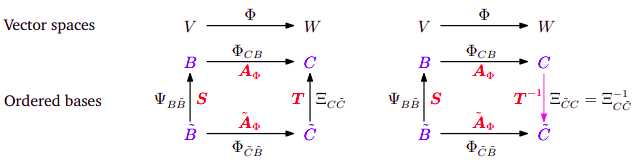
\includegraphics[
        width=\linewidth, 
        height=4cm,
        keepaspectratio,
    ]{images/maths-for-ml/basis-change.png}
    \caption*{
        For a homomorphism $\Phi  : V \to  W$ and ordered bases $B, \tilde{B}$ of $V$ and $C, \tilde{C}$ of $W$ (marked in \textcolor{blue}{blue}), we can express the mapping $\Phi _{\tilde{C} \tilde{B}}$ with respect to the bases $\tilde{B}, \tilde{C}$ equivalently as a composition of the homomorphisms $\Phi _{\tilde{C} \tilde{B}} = \Xi _{\tilde{C}C} \circ \Phi _{CB} \circ \Psi _{B\tilde{B}}$ with respect to the bases in the subscripts. 
        \\
        The corresponding transformation matrices are in \textcolor{red}{red}.
        \\
        We use $\Psi_{B\tilde{B}} = \text{id}_V$ and $\Xi _{C\tilde{C}} = \text{id}_W$ , i.e., the identity mappings that map vectors onto themselves, but with respect to a different basis.
        \hfill \cite{mfml/book/mml/Deisenroth-Faisal-Ong}
    }
\end{figure}


\begin{enumerate}
    \item \textbf{Theorem}: For a linear mapping $\Phi : V \to W$, ordered bases
    \hfill \cite{mfml/book/mml/Deisenroth-Faisal-Ong}
    \\
    .\hfill
    $
        B = (\bm{b}_1, \cdots , \bm{b}_n), \ 
        \tilde{B} = (\tilde{\bm{b}}_1, \cdots , \tilde{\bm{b}}_n)
    $
    \hfill \cite{mfml/book/mml/Deisenroth-Faisal-Ong}
    \\
    of $V$ and
    \hfill \cite{mfml/book/mml/Deisenroth-Faisal-Ong}
    \\
    .\hfill
    $
        C = (\bm{c}_1, \cdots , \bm{c}_n), \ 
        \tilde{C} = (\tilde{\bm{c}}_1, \cdots , \tilde{\bm{c}}_n)
    $
    \hfill \cite{mfml/book/mml/Deisenroth-Faisal-Ong}
    \\
    of $W$, and a transformation matrix $\bm{A}_\Phi$ of $\Phi$ with respect to $B$ and $C$, the corresponding transformation matrix $\tilde{\bm{A}} _\Phi$ with respect to the bases $\tilde{B}$ and $\tilde{C}$ is given as
    $
        \tilde{\bm{A}} \Phi = \bm{T}^{-1}\bm{A}_\Phi \bm{S}
    $.
    \hfill \cite{mfml/book/mml/Deisenroth-Faisal-Ong}
    \\
    Here, $\bm{S} \in \mathbb{R}^{n\times n}$ is the transformation matrix of $\text{id}_V$ that maps coordinates with respect to $\tilde{B}$ onto coordinates with respect to $B$, \ 
    and $\bm{T} \in \mathbb{R}^{m\times m}$ is the transformation matrix of $\text{id}_W$ that maps coordinates with respect to $\tilde{C}$ onto coordinates with respect to $C$.
    \hfill \cite{mfml/book/mml/Deisenroth-Faisal-Ong}

    \item \textbf{Proof}: we can write the vectors of the new basis $\tilde{B}$ of $V$ as a linear combination of the basis vectors of $B$, such that:
    \hfill \cite{mfml/book/mml/Deisenroth-Faisal-Ong}
    \\
    .\hfill
    $
        \tilde{\bm{b}}_j 
        = s_{1j} \bm{b}_1 + \cdots + s_{nj} \bm{b}_n 
        = \dsum^n _{i=1} s_{ij} \bm{b}_i 
        , j = 1, \cdots , n
    $
    \hfill \cite{mfml/book/mml/Deisenroth-Faisal-Ong}
    \\
    Similarly, we write the new basis vectors $\tilde{C}$ of $W$ as a linear combination of the basis vectors of $C$, which yields
    \hfill \cite{mfml/book/mml/Deisenroth-Faisal-Ong}
    \\
    .\hfill
    $
        \tilde{\bm{c}}_k 
        = t_{1k} \bm{c}_1 + \cdots + t_{mk} \bm{c}_m 
        = \dsum^m _{l=1} t_{lk} \bm{c}_l 
        , k = 1, \cdots , m
    $
    \hfill \cite{mfml/book/mml/Deisenroth-Faisal-Ong}
    \\
    We define $\bm{S} = ((s_{ij} )) \in \mathbb{R}^{n\times n}$ as the transformation matrix that maps coordinates with respect to $\tilde{B}$ onto coordinates with respect to $B$ and $\bm{T} = ((t_{lk})) \in R^{m\times m}$ as the transformation matrix that maps coordinates with respect to $\tilde{C}$ onto coordinates with respect to $C$. 
    In particular, the $j$-th column of $\bm{S}$ is the coordinate representation of $\tilde{\bm{b}}_j$ with respect to $B$ and the $k$-th column of $\bm{T}$ is the coordinate representation of $\tilde{\bm{c}}_k$ with respect to $C$. 
    Note that both $\bm{S}$ and $\bm{T}$ are regular.
    \hfill \cite{mfml/book/mml/Deisenroth-Faisal-Ong}
    \\
    We are going to look at $\Phi(\tilde{\bm{b}}_j )$ from two perspectives.
    \hfill \cite{mfml/book/mml/Deisenroth-Faisal-Ong}
    \begin{enumerate}
        \item Applying the mapping $\Phi$, we get that for all $j = 1, \cdots , n$
        \hfill \cite{mfml/book/mml/Deisenroth-Faisal-Ong}
        \\
        .\hfill
        $
            \Phi(\tilde{\bm{b}}_j )
            = \dsum^m_{k=1} \underset{\displaystyle \in W}{
                \underbrace{\tilde{a}_{kj} \textcolor{blue}{\tilde{\bm{c}}_k}}
            }
            = \dsum^m_{k=1} \tilde{a}_{kj} \textcolor{blue}{
                \dsum^m_{l=1} t_{lk} \bm{c}_l
            }
            = \dsum^m_{l=1} \dParenBrac{
                \textcolor{PineGreen}{\dsum^m_{k=1} t_{lk} \tilde{a}_{kj}} 
            }  \bm{c}_l
        $
        \hfill \cite{mfml/book/mml/Deisenroth-Faisal-Ong}
        \\
        where we first expressed the new basis vectors $\tilde{\bm{c}}_k \in W$ as linear combinations of the basis vectors $\bm{c}_l \in W$ and then swapped the order of summation.
        \hfill \cite{mfml/book/mml/Deisenroth-Faisal-Ong}


        \item when we express the $\tilde{\bm{b}}_j \in V$ as linear combinations of $\bm{b}_j \in V$ , we arrive at ($j = 1,\cdots, n$) :
        \hfill \cite{mfml/book/mml/Deisenroth-Faisal-Ong}
        \\
        .\hfill
        $
            \Phi (\tilde{\bm{b}}_j ) 
            = \Phi  \dParenBrac{ \textcolor{blue}{\dsum ^n _{i=1} s_{ij} \bm{b}_i}}
            = \dsum ^n _{i=1} s_{ij} \textcolor{red}{\Phi (\bm{b}_i)} 
            = \dsum^n _{i=1} s_{ij} \textcolor{red}{\dsum ^m _{l=1} a_{li} \bm{c}_l}
            = \dsum ^m _{l=1} \dParenBrac{ \textcolor{PineGreen}{\dsum^n _{i=1} s_{ij} a_{li}} } \bm{c}_l
        $
        \hfill \cite{mfml/book/mml/Deisenroth-Faisal-Ong}

        \item $
            \begin{aligned}
                \dsum^m_{k=1} t_{lk} \tilde{a}_{kj} = \dsum^n _{i=1} s_{ij} a_{li}
                \hspace{1cm}
                \Rightarrow 
                \bm{T} \tilde{\bm{A}}_\Phi = \bm{A}_\Phi \bm{S} 
                \in \mathbb{R}^{m\times n}
                \hspace{1cm}
                \Rightarrow 
                \tilde{\bm{A}}_\Phi = \bm{T}^{-1} \bm{A}_\Phi \bm{S}
            \end{aligned}
        $
        \hfill \cite{mfml/book/mml/Deisenroth-Faisal-Ong}        
    \end{enumerate}

    
\end{enumerate}






\subsection{Orthonormal Basis}


\begin{enumerate}
    \item 
\end{enumerate}




























\section{Linear Mappings}


\begin{figure}[H]
    \centering
    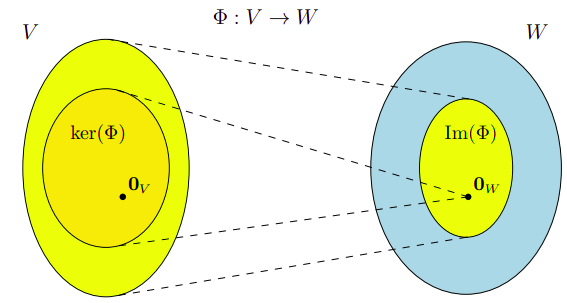
\includegraphics[
        width=\linewidth,
        height=4cm,
        keepaspectratio,
    ]{images/maths-for-ml/image-kernel-linear-mapping.png}
\end{figure}

\begin{enumerate}
    \item \textbf{Definition}: For vector spaces $V, W$, a mapping $\Phi : V \to W$ is called a linear mapping (or vector space homomorphism/ linear transformation) if
    \hfill \cite{mfml/book/mml/Deisenroth-Faisal-Ong}
    \\
    .\hfill
    $
        \forall \bm{x}, \bm{y} \in V \forall \lambda , \psi  \in \mathbb{R} : 
        \Phi(\lambda \bm{x} + \psi \bm{y}) = \lambda \Phi(\bm{x}) + \psi \Phi(\bm{y})
    $
    \hfill \cite{mfml/book/mml/Deisenroth-Faisal-Ong}

    \item we can represent linear mappings as matrices
    \hfill \cite{mfml/book/mml/Deisenroth-Faisal-Ong}

    \item For linear mappings $\Phi : V \to W$ and $\Psi : W \to X$, the mapping $\Psi \circ \Phi : V \to X$ is also linear.
    \hfill \cite{mfml/book/mml/Deisenroth-Faisal-Ong}

    \item If $\Phi : V \to W, \Psi : V \to W$ are linear, then $\Phi + \Psi$ and $\lambda\Phi, \lambda \in \mathbb{R}$, are linear, too.
    \hfill \cite{mfml/book/mml/Deisenroth-Faisal-Ong}
\end{enumerate}



\subsection{Matrix Representation of Linear Mappings}

\begin{enumerate}
    \item Any $n$-dimensional vector space is isomorphic to $\mathbb{R}^n$.
    \hfill \cite{mfml/book/mml/Deisenroth-Faisal-Ong}

    \item We consider a basis $\dCurlyBrac{\bm{b}_1, \cdots , \bm{b}_n}$ of an $n$-dimensional vector space $V$ .
    \hfill \cite{mfml/book/mml/Deisenroth-Faisal-Ong}
\end{enumerate}




\subsection{Image/Range \& Kernel/Null space}

\begin{enumerate}
    \item \textbf{Definition}: For $\Phi  : V \to W$, we define the image/range
    \hfill \cite{mfml/book/mml/Deisenroth-Faisal-Ong}
    \\
    .\hfill
    $
        \text{Im}(\Phi ) 
        := \Phi (V ) 
        = \dCurlyBrac{\bm{w} \in W|\exists \bm{v} \in V : \Phi (\bm{v}) = \bm{w}}
    $
    \hfill \cite{mfml/book/mml/Deisenroth-Faisal-Ong}

    \item \textbf{Definition}: For $\Phi  : V \to W$, we define the kernel/null space
    \hfill \cite{mfml/book/mml/Deisenroth-Faisal-Ong}
    \\
    .\hfill
    $
        \ker(\Phi ) 
        := \Phi ^{-1} (\bm{0}_W ) 
        = \dCurlyBrac{\bm{v} \in V : \Phi (\bm{v}) = \bm{0}_W }
    $
    \hfill \cite{mfml/book/mml/Deisenroth-Faisal-Ong}


    \item We also call $V$ and $W$ also the \textbf{domain} and \textbf{codomain} of $\Phi$, respectively.
    \hfill \cite{mfml/book/mml/Deisenroth-Faisal-Ong}

    \item The image is the set of vectors $\bm{w} \in W$ that can be “reached” by $\Phi$ from any vector in $V$ .
    \hfill \cite{mfml/book/mml/Deisenroth-Faisal-Ong}

    \item Intuitively, the kernel is the set of vectors $\bm{v} \in V$ that $\Phi$ maps onto the neutral element $\bm{0}_W \in W$.
    \hfill \cite{mfml/book/mml/Deisenroth-Faisal-Ong}

    \item It always holds that $\Phi(\bm{0}_V ) = \bm{0}_W$ and, therefore, $\bm{0}_V \in \ker(\Phi)$. 
    In particular, the null space is never empty.
    \hfill \cite{mfml/book/mml/Deisenroth-Faisal-Ong}

    \item $Im(\Phi) \subseteq W$ is a subspace of $W$, and $\ker(\Phi) \subseteq V$ is a subspace of $V$ .
    \hfill \cite{mfml/book/mml/Deisenroth-Faisal-Ong}

    \item $\Phi$ is injective (one-to-one) if and only if $\ker(\Phi) = \dCurlyBrac{\bm{0}}$.
    \hfill \cite{mfml/book/mml/Deisenroth-Faisal-Ong}

    \item \textbf{Rank-Nullity Theorem}: For vector spaces $V, W$ and a linear mapping $\Phi : V \to W$ it holds that $\dim(\ker(\Phi)) + \dim(\text{Im}(\Phi)) = \dim(V )$.
    \hfill \cite{mfml/book/mml/Deisenroth-Faisal-Ong}
    \begin{enumerate}
        \item The rank-nullity theorem is also referred to as the \textbf{fundamental theorem of linear mappings}
        \hfill \cite{mfml/book/mml/Deisenroth-Faisal-Ong}

        \item If $\dim(\text{Im}(\Phi )) < \dim(V )$, then $\ker(\Phi)$ is non-trivial, i.e., the kernel contains more than $\bm{0}_V$ and $\dim(\ker(\Phi)) \geq 1$.
        \hfill \cite{mfml/book/mml/Deisenroth-Faisal-Ong}

        \item If $\bm{A}_\Phi $ is the transformation matrix of $\Phi$  with respect to an ordered basis and $\dim(\text{Im}(\Phi )) < \dim(V )$, then the system of linear equations $\bm{A}_\Phi \bm{x} = \bm{0}$ has infinitely many solutions.
        \hfill \cite{mfml/book/mml/Deisenroth-Faisal-Ong}

        \item If $\dim(V ) = \dim(W)$, then the following three-way equivalence holds:
        \begin{enumerate}
            \item $\Phi$ is injective
            \item $\Phi$ is surjective
            \item $\Phi$ is bijective
        \end{enumerate}
        since $\text{Im}(\Phi) \subseteq W$.
    \end{enumerate}
\end{enumerate}













\section{Affine Mapping}

\begin{enumerate}
    \item \textbf{Definition}: For two vector spaces $V, W$, a linear mapping $\Phi : V \to W$, and $\bm{a} \in W$, the mapping:
    \hfill \cite{mfml/book/mml/Deisenroth-Faisal-Ong}
    \\
    .\hfill
    $ \phi : V \to W $ such that $ \bm{x} \mapsto \bm{a} + \Phi(\bm{x}) $
    \hfill \cite{mfml/book/mml/Deisenroth-Faisal-Ong}
    \\
    is an affine mapping from $V$ to $W$. 
    The vector a is called the \textbf{translation vector} of $\phi$.
    \hfill \cite{mfml/book/mml/Deisenroth-Faisal-Ong}

    \item Every affine mapping $\phi  : V \to W$ is also the composition of a linear mapping $\phi  : V \to W$ and a translation $\tau : W \to W$ in $W$, such that $\phi  = \tau \circ \phi $. 
    The mappings $\phi $ and $\tau$ are uniquely determined.
    \hfill \cite{mfml/book/mml/Deisenroth-Faisal-Ong}

    \item The composition $\phi ^\prime \circ \phi $ of affine mappings $\phi  : V \to W, \phi ^\prime: W \to X$ is affine.
    \hfill \cite{mfml/book/mml/Deisenroth-Faisal-Ong}

    \item Affine mappings keep the geometric structure invariant. 
    They also preserve the dimension and parallelism.
    \hfill \cite{mfml/book/mml/Deisenroth-Faisal-Ong}
\end{enumerate}



























\section{Injective, Surjective, Bijective Mappings}

\textbf{Definition}: Consider a mapping $\Phi : \mathcal{V} \to \mathcal{W}$, where $\mathcal{V}, \mathcal{W}$ can be arbitrary sets. 
Then $\Phi$ is called:
\hfill \cite{mfml/book/mml/Deisenroth-Faisal-Ong}

\begin{enumerate}
    \item \textbf{Injective} if $\forall \bm{x}, \bm{y} \in \mathcal{V} : \Phi(\bm{x}) = \Phi(\bm{y}) \Rightarrow \bm{x} = \bm{y}$
    \hfill \cite{mfml/book/mml/Deisenroth-Faisal-Ong}

    \item \textbf{Surjective} if $\Phi(\mathcal{V}) = \mathcal{W}$
    \hfill \cite{mfml/book/mml/Deisenroth-Faisal-Ong}
    \begin{enumerate}
        \item If $\Phi$ is surjective, then every element in $\mathcal{W}$ can be “reached” from $\mathcal{V}$ using $\Phi$.
        \hfill \cite{mfml/book/mml/Deisenroth-Faisal-Ong}
    \end{enumerate}
    
    \item \textbf{Bijective} if it is injective and surjective
    \hfill \cite{mfml/book/mml/Deisenroth-Faisal-Ong}
    \begin{enumerate}
        \item A bijective $\Phi$ can be “undone”, i.e., there exists a mapping $\Psi : W \to V$ so that $\Psi \circ \Phi(\bm{x}) = \bm{x}$.
        \hfill \cite{mfml/book/mml/Deisenroth-Faisal-Ong}

        \item This mapping $\Psi$ is then called the inverse of $\Phi$ and normally denoted by $\Phi^{-1}$.
        \hfill \cite{mfml/book/mml/Deisenroth-Faisal-Ong}
    \end{enumerate}    

\end{enumerate}


















\section{Special cases of Linear mappings}

\textbf{Definition}: Consider a mapping $\Phi : V \to W$, where $V, W$ can be arbitrary vector spaces. 
Then:
\hfill \cite{mfml/book/mml/Deisenroth-Faisal-Ong}

\begin{enumerate}
    \item \textbf{Isomorphism}: $\Phi : V \to W$ linear and bijective
    \hfill \cite{mfml/book/mml/Deisenroth-Faisal-Ong}
    \begin{enumerate}
        \item \textbf{Theorem}: Finite-dimensional vector spaces $V$ and $W$ are isomorphic if and only if $\dim(V ) = \dim(W)$.
        \hfill \cite{mfml/book/mml/Deisenroth-Faisal-Ong}

        \item there exists a linear, bijective mapping between two vector spaces of the same dimension.
        Intuitively, this means that vector spaces of the same dimension are kind of the same thing, as they can be transformed into each other without incurring any loss.
        \hfill \cite{mfml/book/mml/Deisenroth-Faisal-Ong}

        \item It gives the justification to treat $\mathbb{R}^{m\times n}$ (the vector space of $m \times n$-matrices) and $\mathbb{R}^{mn}$ (the vector space of vectors of length $mn$) the same, as their dimensions are $mn$, and there exists a linear, bijective mapping that transforms one into the other.
        \hfill \cite{mfml/book/mml/Deisenroth-Faisal-Ong}

        \item If $\Phi : V \to W$ is an isomorphism, then $\Phi ^{-1} : W \to V$ is an isomorphism, too.
        \hfill \cite{mfml/book/mml/Deisenroth-Faisal-Ong}
    \end{enumerate}

    \item \textbf{Endomorphism}: $\Phi : V \to V$ linear
    \hfill \cite{mfml/book/mml/Deisenroth-Faisal-Ong}

    \item \textbf{Automorphism}: $\Phi : V \to V$ linear and bijective
    \hfill \cite{mfml/book/mml/Deisenroth-Faisal-Ong}

    \item \textbf{identity mapping} or \textbf{identity automorphism}: $id_V : V \to V , \bm{x} \mapsto \bm{x}$
    \hfill \cite{mfml/book/mml/Deisenroth-Faisal-Ong}
\end{enumerate}



















\section{Transformation Matrix ( $A_\Phi$ )}

\begin{enumerate}
    \item \textbf{Definition}: Consider vector spaces $V$, $W$ with corresponding (ordered) bases $B = (\bm{b}_1, \cdots , \bm{b}_n)$ and $C = (\bm{c}_1, \cdots , \bm{c}_m)$. 
    Moreover, we consider a linear mapping $\Phi : V \to W$. 
    For $j \in \dCurlyBrac{1, \cdots , n}$,
    \hfill \cite{mfml/book/mml/Deisenroth-Faisal-Ong}
    \\
    .\hfill
    $
        \Phi(\bm{b}_j ) = \alpha _{1j} \bm{c}_1 + \cdots + \alpha _{mj} \bm{c}_m 
        = \dsum^m_{i=1} \alpha _{ij} \bm{c}_i
    $
    \hfill \cite{mfml/book/mml/Deisenroth-Faisal-Ong}
    \\
    is the unique representation of $\Phi(\bm{b}_j )$ with respect to $C$. 
    Then, we call the $m \times n$-matrix $\bm{A}_\Phi$, whose elements are given by $\bm{A}_\Phi(i, j) = \alpha_{ij}$ the transformation matrix of $\Phi$ (with respect to the ordered bases $B$ of $V$ and $C$ of $W$  ).
    \hfill \cite{mfml/book/mml/Deisenroth-Faisal-Ong}

    \item The transformation matrix can be used to map coordinates with respect to an ordered basis in $V$ to coordinates with respect to an ordered basis in $W$.
    \hfill \cite{mfml/book/mml/Deisenroth-Faisal-Ong}

    \item Consider vector spaces $V, W, X$. 
    We already know that for linear mappings $\Phi  : V \to  W$ and $\Psi : W \to  X$ the mapping $\Psi \circ \Phi  : V \to  X$ is also linear. 
    With transformation matrices $\bm{A}_\Phi$  and $\bm{A}_\Psi$ of the corresponding mappings, the overall transformation matrix is $\bm{A}_{\Psi\circ\Phi}  = \bm{A}_\Psi \bm{A}_\Phi$ .
    \hfill \cite{mfml/book/mml/Deisenroth-Faisal-Ong}

    \item 
    $\bm{A}_\Phi$  is the transformation matrix of a linear mapping $\Phi _{CB} : V \to  W$ with respect to the bases $B, C$.
    \hfill \cite{mfml/book/mml/Deisenroth-Faisal-Ong}
    \\[0.2cm]
    $\tilde{\bm{A}}_\Phi$  is the transformation matrix of the linear mapping $\Phi_ {\tilde{C}\tilde{B}} : V \to  W$ with respect to the bases $\tilde{B}, \tilde{C}$.
    \hfill \cite{mfml/book/mml/Deisenroth-Faisal-Ong}
    \\[0.2cm]
    $\bm{S}$ is the transformation matrix of a linear mapping $\Psi _{B\tilde{B}} : V \to  V$ (automorphism) that represents $\tilde{B}$ in terms of $B$. Normally, $\Psi  = \text{id}_V$ is the identity mapping in $V$ .
    \hfill \cite{mfml/book/mml/Deisenroth-Faisal-Ong}
    \\[0.2cm]
    $\bm{T}$ is the transformation matrix of a linear mapping $\Xi _{C\tilde{C}} : W \to  W$ (automorphism) that represents $\tilde{C}$ in terms of $C$. Normally, $\Xi  = \text{id}_W$ is the identity mapping in $W$.
    \hfill \cite{mfml/book/mml/Deisenroth-Faisal-Ong}
    \\[0.2cm]
    If we (informally) write down the transformations just in terms of bases, then $\bm{A}_\Phi  : B \to  C$, $\tilde{\bm{A}}_\Phi  : \tilde{B} \to  \tilde{C}$, $\bm{S} : \tilde{B} \to  B$, $\bm{T} : \tilde{C} \to  C$ and $\bm{T}^{-1} : C \to  \bm{C}$, and
    \hfill \cite{mfml/book/mml/Deisenroth-Faisal-Ong}
    \\[0.2cm]
    .\hfill
    $
        \tilde{B} \to  \tilde{C} = \textcolor{blue}{\tilde{B} \to  B} \textcolor{red}{\to  C} \to  \tilde{C} 
        \Rightarrow
        \tilde{\bm{A}}_\Phi  = \bm{T}^{-1} \textcolor{red}{\bm{A}_\Phi} \textcolor{blue}{\bm{S}}
    $
    \hfill \cite{mfml/book/mml/Deisenroth-Faisal-Ong}
    \\[0.2cm]
    Note that the execution order is from \textbf{right to left} because vectors are multiplied at the right-hand side so that 
    \hfill \cite{mfml/book/mml/Deisenroth-Faisal-Ong}
    \\[0.2cm]
    .\hfill
    $\bm{x} \mapsto  \bm{Sx} \mapsto  \bm{A}_\Phi (\bm{Sx}) \mapsto \bm{T}^{-1}(\bm{A}_\Phi (\bm{Sx})) = \tilde{\bm{A}}_\Phi \bm{x}$.
    \hfill \cite{mfml/book/mml/Deisenroth-Faisal-Ong}

    \item  Orthogonal matrices define transformations that are rotations (with the possibility of flips).
    \hfill \cite{mfml/book/mml/Deisenroth-Faisal-Ong}
\end{enumerate}






\section{Coordinates}

\begin{enumerate}
    \item Consider a vector space $V$ and an ordered basis $B = (\bm{b}_1, \cdots , \bm{b}_n)$ of $V$ . 
    For any $\bm{x} \in V$ we obtain a unique representation (linear combination):
    \hfill \cite{mfml/book/mml/Deisenroth-Faisal-Ong}
    \\
    .\hfill
    $
        \bm{x} = \alpha_1 \bm{b}_1 + \cdots + \alpha_n \bm{b}_n
    $
    \hfill \cite{mfml/book/mml/Deisenroth-Faisal-Ong}
    \\
    of $\bm{x}$ with respect to $B$. 
    Then $\alpha_1, \cdots , \alpha_n$ are the coordinates of $\bm{x}$ with respect to $B$, and the vector:
    \hfill \cite{mfml/book/mml/Deisenroth-Faisal-Ong}
    \\
    .\hfill
    $
        \bm{\alpha} = \begin{bmatrix}
            \alpha_1 \\
            \vdots \\
            \alpha_n
        \end{bmatrix}
        \in \mathbb{R}^n
    $
    \hfill \cite{mfml/book/mml/Deisenroth-Faisal-Ong}
    \\
    is the \textbf{coordinate vector/ coordinate} representation of $\bm{x}$ with respect to the ordered basis $B$.
    \hfill \cite{mfml/book/mml/Deisenroth-Faisal-Ong}

    \item A basis effectively defines a coordinate system.
    \hfill \cite{mfml/book/mml/Deisenroth-Faisal-Ong}

    \item For an $n$-dimensional vector space $V$ and an ordered basis $B$ of $V$ , the mapping $\Phi : \mathbb{R}^n \to V , \Phi(\bm{e}_i) = \bm{b}_i , i = 1, \cdots , n$, is linear, where $(\bm{e}_1, \cdots , \bm{e}_n)$ is the standard basis of $\mathbb{R}^n$.
    \hfill \cite{mfml/book/mml/Deisenroth-Faisal-Ong}

    \item The coordinates of $\Phi(\bm{b}_j )$ with respect to the ordered basis $C$ of $W$ are the $j$-th column of $\bm{A}_\Phi$.
    \hfill \cite{mfml/book/mml/Deisenroth-Faisal-Ong}
    \hfill \cite{mfml/book/mml/Deisenroth-Faisal-Ong}
    \begin{enumerate}
        \item Consider (finite-dimensional) vector spaces $V$, $W$ with ordered bases $B$, $C$ and a linear mapping $\Phi : V \to W$ with transformation matrix $\bm{A}_\Phi$.
        \hfill \cite{mfml/book/mml/Deisenroth-Faisal-Ong}

        \item If $\hat{\bm{x}}$ is the coordinate vector of $\bm{x} \in V$ with respect to $B$ and $\hat{\bm{y}}$ the coordinate vector of $\bm{y} = \Phi(\bm{x}) \in W$ with respect to $C$, then $\hat{\bm{y}} = \bm{A}_\Phi \hat{\bm{x}}$.
        \hfill \cite{mfml/book/mml/Deisenroth-Faisal-Ong}
    \end{enumerate}    
\end{enumerate}




























\chapter{Vector Calculus}

\section{Function ($f(x)$)}

\begin{enumerate}
    \item A function $f$ is a quantity that relates two quantities to each other. 
    \hfill \cite{mfml/book/mml/Deisenroth-Faisal-Ong}

    \item These quantities are typically inputs $\bm{x} \in \mbbR^D$ and targets (function values) $f (\bm{x})$, which we assume are real-valued if not stated otherwise. 
    \hfill \cite{mfml/book/mml/Deisenroth-Faisal-Ong}
    
    \item $\mbbR^D$ is the domain of $f$ , and the function values $f (\bm{x})$ are the image/codomain of $f$ .
    \hfill \cite{mfml/book/mml/Deisenroth-Faisal-Ong}

    \item We often write 
    \hfill \cite{mfml/book/mml/Deisenroth-Faisal-Ong}
    \begin{enumerate}
        \item $f: \mbbR^D \to \mbbR$ 
        (specifies that $f$ is a mapping from $\mbbR^D$ to $\mbbR$ )
        \hfill \cite{mfml/book/mml/Deisenroth-Faisal-Ong}
        
        \item $\bm{x} \mapsto f(\bm{x})$ 
        (specifies the explicit assignment of an input $\bm{x}$ to a function value $f(\bm{x})$)
        \hfill \cite{mfml/book/mml/Deisenroth-Faisal-Ong}
    \end{enumerate}
    to specify a function.
    \hfill \cite{mfml/book/mml/Deisenroth-Faisal-Ong}

    \item A function $f$ assigns every input x exactly one function value $f (\bm{x})$.
    \hfill \cite{mfml/book/mml/Deisenroth-Faisal-Ong}
\end{enumerate}

\vspace{0.5cm}
\textbf{ALSO SEE/ RELATED}:
\begin{enumerate}
    \item \fullref{vector space/Linear Mappings}
\end{enumerate}



\subsection{Differentiation of Uni-variate Functions}

\begin{enumerate}
    \item 
    \begin{definition}[Univariate function ($f : \mbbR \to \mbbR$)]
        Univariate function: $y = f(x),\ x, y \in \mbbR$
        \hfill \cite{mfml/book/mml/Deisenroth-Faisal-Ong}
    \end{definition}

    \item 
    \begin{definition}[Difference Quotient]
        The difference quotient
        $
            \dfrac{\delta y}{\delta x} 
            := \dfrac{f(x + \delta x) - f(x)}{\delta x}
        $
        computes the slope of the secant line through two points on the graph of $f$ .
        \hfill \cite{mfml/book/mml/Deisenroth-Faisal-Ong}
    \end{definition}

    \item The derivative of $f$ points in the direction of steepest ascent of $f$. 
    \hfill \cite{mfml/book/mml/Deisenroth-Faisal-Ong}

    \item 
    \begin{definition}[Taylor Polynomial ( $T_n(x)$ )]
        The Taylor polynomial of degree $n$ of $f : \mbbR \to \mbbR$ at $x_0$ is defined as
        $
            T_n(x)
            := \dsum_{k=0}^n \dfrac{f^{(k)}(x_0)}{k!} (x - x_0)^k
        $
        \hfill \cite{mfml/book/mml/Deisenroth-Faisal-Ong}
        \\
        where $f ^{(k)}(x_0)$ is the $k$-th derivative of $f$ at $x_0$ (which we assume exists) and $\dfrac{f ^{(k)}(x_0)}{ k!}$ are the coefficients of the polynomial.
        \hfill \cite{mfml/book/mml/Deisenroth-Faisal-Ong}
        \\
        We define $t^0 := 1$ for all $t \in \mbbR$.
        \hfill \cite{mfml/book/mml/Deisenroth-Faisal-Ong}
    \end{definition}
    \begin{enumerate}
        \item In general, a Taylor polynomial of degree $n$ is an \textbf{approximation} of a function, which does not need to be a polynomial. 
        The Taylor polynomial is similar to $f$ in a neighborhood around $x_0$. 
        Higher-order Taylor polynomials approximate the function $f$ better and more globally.
        \hfill \cite{mfml/book/mml/Deisenroth-Faisal-Ong}
        
        \item A Taylor polynomial of degree $n$ is an \textbf{exact} representation of a polynomial $f$ of degree $k \leq n$ since all derivatives $f (i)$, $i > k$ vanish. 
        \hfill \cite{mfml/book/mml/Deisenroth-Faisal-Ong}
    \end{enumerate}


    \item 
    \begin{definition}[Power Series]
        $
            f(x) = \dsum_{k=0}^{\infty} a_k (x-c)^k
        $
        \\
        where $a_k$ are coefficients and $c$ is a constant
    \end{definition}


    \item 
    \begin{definition}[Taylor Series ($T_{\infty}(x)$)]
        For a smooth function $f \in C^{\infty}$, $f : \mbbR \to \mbbR$, the Taylor series of $f$ at $x_0$ is defined as
        $
            T_{\infty}(x)
            = \dsum_{k=0}^{\infty} \dfrac{f^{(k)}(x_0)}{k!} (x - x_0)^k
        $
        \hfill \cite{mfml/book/mml/Deisenroth-Faisal-Ong}
        \\
         $f \in C^{\infty}$ means that $f$ is continuously differentiable infinitely many times
         \hfill \cite{mfml/book/mml/Deisenroth-Faisal-Ong}
    \end{definition}
    \begin{enumerate}
        \item 
        \begin{definition}[Maclaurin series]        
            For $x_0 = 0$, we obtain the \textbf{Maclaurin series} as a special instance of the Taylor series. 
            \hfill \cite{mfml/book/mml/Deisenroth-Faisal-Ong}
        \end{definition}

        \item 
        \begin{definition}[Analytic]        
            If $f (x) = T_{\infty}(x)$, then $f$ is called \textbf{analytic}.
            \hfill \cite{mfml/book/mml/Deisenroth-Faisal-Ong}
        \end{definition}
    \end{enumerate}
\end{enumerate}




\subsection{Differentiation of multi-variate Functions}

\begin{enumerate}
    \item 
    \begin{definition}[multi-variate Functions ($f : \mbbR^n \to \mbbR$)]
        The general case where the function $f$ depends on one or more variables $\bm{x} \in \mbbR^n$
        \hfill \cite{mfml/book/mml/Deisenroth-Faisal-Ong}
    \end{definition}

    \item 
    \begin{definition}[Partial Derivative ($\dfrac{\partial f}{\partial x_i}$)]
        For a function $f : \mbbR^n \to \mbbR$, $\bm{x} \mapsto f (\bm{x})$, $\bm{x} \in \mbbR^n$ of $n$ variables $x_1, \cdots , x_n$ we define the partial derivatives as
        \hfill \cite{mfml/book/mml/Deisenroth-Faisal-Ong}
        \\
        .\hfill
        ${
            \displaystyle
            \begin{matrix}
                \dfrac{\partial f}{\partial x_1} 
                & 
                = 
                & 
                \lim_{h\to 0} \dfrac{f (x_1 + h, x_2, \cdots , x_n) - f (\bm{x})}{h}
                \\
                & \vdots &
                \\
                \dfrac{\partial f}{\partial x_n} 
                & 
                = 
                & 
                \lim_{h\to 0} \dfrac{f (x_1 , x_2, \cdots , x_n+ h) - f (\bm{x})}{h}
            \end{matrix}
        }$
        \hfill \cite{mfml/book/mml/Deisenroth-Faisal-Ong}
    \end{definition}
\end{enumerate}

\subsubsection{Gradient}

\begin{enumerate}
    \item The generalization of the derivative to functions of several variables is the \textbf{gradient}.
    \hfill \cite{mfml/book/mml/Deisenroth-Faisal-Ong}

    \item We find the gradient of the function $f$ with respect to $\bm{x}$ by varying one variable at a time and keeping the others constant. 
    \hfill \cite{mfml/book/mml/Deisenroth-Faisal-Ong}
    
    \item The gradient is then the \textbf{collection} of these partial derivatives.
    \hfill \cite{mfml/book/mml/Deisenroth-Faisal-Ong}

    \item 
    \begin{definition}[Gradient ($\nabla_x f \in \mbbR^{1 \times n}$)]
        For a function $f : \mbbR^n \to \mbbR$, $\bm{x} \mapsto f (\bm{x})$, $\bm{x} \in \mbbR^n$ of $n$ variables $x_1, \cdots , x_n$:
        \\
        .\hfill
        $
            \nabla_x f
            = \text{grad} f
            = \dfrac{df}{d\bm{x}}
            = \begin{bmatrix}
                \dfrac{\partial f(\bm{x})}{\partial x_1} &
                \dfrac{\partial f(\bm{x})}{\partial x_2} &
                \cdots
                \dfrac{\partial f(\bm{x})}{\partial x_n}
            \end{bmatrix}
            \in \mbbR^{1 \times n}
        $
        \hfill \cite{mfml/book/mml/Deisenroth-Faisal-Ong}
        \\
        where $n$ is the number of variables and $1$ is the dimension of the image/range/codomain of $f$ .
        The row vector is called the gradient of $f$ or the Jacobian.
        \hfill \cite{mfml/book/mml/Deisenroth-Faisal-Ong}
    \end{definition}

    \item This definition of Jacobian is a special case of the general definition of the Jacobian for vector-valued functions as the collection of partial derivatives.
    \hfill \cite{mfml/book/mml/Deisenroth-Faisal-Ong}

    \item The reason why we define the gradient vector as a row vector:
    \hfill \cite{mfml/book/mml/Deisenroth-Faisal-Ong}
    \begin{enumerate}
        \item we can consistently generalize the gradient to vector-valued functions $f : \mbbR^n \to \mbbR^m$ (then the gradient becomes a matrix)
        \hfill \cite{mfml/book/mml/Deisenroth-Faisal-Ong}

        \item we can immediately apply the multi-variate chain rule without paying attention to the dimension of the gradient.
        \hfill \cite{mfml/book/mml/Deisenroth-Faisal-Ong}
    \end{enumerate}
\end{enumerate}






\section{Gradients of Vector-Valued Functions ($J = \nabla_x f$)}

\begin{enumerate}
    \item 
    \begin{definition}[vector-valued functions/ vector fields ($\bm{f} : \mbbR^n \to \mbbR^m$)]
        vector-valued functions (vector fields) are defined as $\bm{f} : \mbbR^n \to \mbbR^m$, where $n \geq 1$ and $m > 1$.
        For a function $\bm{f} : \mbbR^n \to \mbbR^m$ and a vector $\bm{x} = [x_1, \cdots , x_n]^\top \in \mbbR^n$, the corresponding vector of function values is given as
        $
            \bm{f}(\bm{x})
            = \begin{bmatrix}
                f_1(\bm{x}) \\
                \vdots \\
                f_m(\bm{x})
            \end{bmatrix}
            \in \mbbR^m
        $
        \hfill \cite{mfml/book/mml/Deisenroth-Faisal-Ong}
    \end{definition}

    \item Writing the vector-valued function in this way allows us to view a vector-valued function $\bm{f} : \mbbR^n \to \mbbR^m$ as a vector of functions $[f_1, \cdots , f_m]^\top$, $f_i : \mbbR^n \to \mbbR$ that map onto $\mbbR$. 
    \hfill \cite{mfml/book/mml/Deisenroth-Faisal-Ong}

    \item 
    .\hfill
    ${
        \displaystyle
        \dfrac{\partial\bm{f}}{\partial x_i}
        = \begin{bmatrix}
            \dfrac{\partial f_1}{\partial x_i} \\
            \vdots \\
            \dfrac{\partial f_m}{\partial x_i}
        \end{bmatrix}
        = \begin{bmatrix}
            \lim_{h \to 0} \dfrac{f_1(x_1,\cdots,x_{i-1},x_i+h,x_{i+1},\cdots x_n)-f_1(\bm{x})}{h} \\
            \vdots \\
            \lim_{h \to 0} \dfrac{f_m(x_1,\cdots,x_{i-1},x_i+h,x_{i+1},\cdots x_n)-f_m(\bm{x})}{h}
        \end{bmatrix}
        \in \mbbR^m
    }$
    \hfill \cite{mfml/book/mml/Deisenroth-Faisal-Ong}

    \item 
    \begin{definition}[Jacobian ($\bm{J} = \nabla_{\bm{x}}\bm{f} = \dfrac{d \bm{f}(\bm{x})}{d \bm{x}}$)]
        The collection of all first-order partial derivatives of a vector-valued function $\bm{f} : \mbbR^n \to \mbbR^m$ is called the Jacobian. 
        The Jacobian $\bm{J}$ is an $m \times n$ matrix, which we define and arrange as follows:
        \hfill \cite{mfml/book/mml/Deisenroth-Faisal-Ong}
        \\
        .\hfill
        $
            \bm{J} 
            = \nabla_{\bm{x}}\bm{f}
            = \dfrac{d \bm{f}(\bm{x})}{d \bm{x}}
            = \begin{bmatrix}
                \dfrac{\partial \bm{f}(\bm{x})}{\partial x_1} &
                \cdots &
                \dfrac{\partial \bm{f}(\bm{x})}{\partial x_n}
            \end{bmatrix}
            = \begin{bmatrix}
                \dfrac{\partial f_1(\bm{x})}{\partial x_1} &
                \cdots &
                \dfrac{\partial f_1(\bm{x})}{\partial x_n} \\
                \vdots & \ddots & \vdots \\
                \dfrac{\partial f_m(\bm{x})}{\partial x_1} &
                \cdots &
                \dfrac{\partial f_m(\bm{x})}{\partial x_n} \\
            \end{bmatrix}
            \in \mbbR^{m\times n}
        $
        \hfill \cite{mfml/book/mml/Deisenroth-Faisal-Ong}
        \\
        .\hfill
        $
            \bm{x} = \begin{bmatrix}
                x_1 \\ \cdots \\ x_n
            \end{bmatrix},
            \hspace{1cm}
            J(i,j) = \dfrac{\partial f_i}{\partial x_j}
        $
        \hfill \cite{mfml/book/mml/Deisenroth-Faisal-Ong}
    \end{definition}
    \begin{enumerate}
        \item As a special case, a function $f : \mbbR^n \to \mbbR^1$, which maps a vector $\bm{x} \in \mbbR^n$ onto a scalar (e.g., $f (x) = \dsum^n _{i=1} x_i$), possesses a Jacobian that is a row vector (matrix of dimension $1 \times n$)
        \hfill \cite{mfml/book/mml/Deisenroth-Faisal-Ong}

        \item Jacobian is used in the change-of-variable method for probability distributions. 
        The amount of scaling due to the transformation of a variable is provided by the determinant.
        \hfill \cite{mfml/book/mml/Deisenroth-Faisal-Ong}

        \item The absolute value of the Jacobian determinant $\dabs{det(\bm{J})}$ is the factor by which areas or volumes are scaled when coordinates are transformed.
        \hfill \cite{mfml/book/mml/Deisenroth-Faisal-Ong}

        \item Geometrically, the Jacobian determinant gives the magnification/ scaling factor when we transform an area or volume.
        \hfill \cite{mfml/book/mml/Deisenroth-Faisal-Ong}
    \end{enumerate}

\end{enumerate}







\section{Higher-Order Derivatives}

.\hfill
$
    \dfrac{\partial^2 f}{\partial x^2} = \dfrac{\partial}{\partial x} \dParenBrac{\dfrac{\partial f}{\partial x}}
$
\hfill \vrule \hfill
$
    \dfrac{\partial^2 f}{\partial y \partial x} = \dfrac{\partial}{\partial y} \dParenBrac{\dfrac{\partial f}{\partial x}}
$
\hfill \vrule \hfill
$
    \dfrac{\partial^2 f}{\partial x \partial y} = \dfrac{\partial}{\partial x} \dParenBrac{\dfrac{\partial f}{\partial y}}
$
\hfill \cite{mfml/book/mml/Deisenroth-Faisal-Ong}
\\[0.2cm]
.\hfill
$
    \dfrac{\partial^n f}{\partial x^n} = 
    \dfrac{\partial}{\partial x} \dParenBrac{
        \overset{n \text{ times}}{\cdots} 
        \dParenBrac{\dfrac{\partial}{\partial x} \dParenBrac{\dfrac{\partial f}{\partial x}}}
        \cdots
    }
$
\hfill \cite{mfml/book/mml/Deisenroth-Faisal-Ong}

\begin{enumerate}
    \item 
    \begin{definition}[Hessian ($\bm{H} = \nabla^2_{x,y}f(x,y)$)]    
        The Hessian is the collection of all second-order partial derivatives.
        \hfill \cite{mfml/book/mml/Deisenroth-Faisal-Ong}
    \end{definition}

    \item If $f (x, y)$ is a twice (continuously) differentiable function, then 
    $
        \dfrac{\partial^2 f}{\partial y \partial x}
        = \dfrac{\partial^2 f}{\partial x \partial y}
    $
    \hfill \cite{mfml/book/mml/Deisenroth-Faisal-Ong}

    \item 
    $
        \bm{H}
        = \nabla^2_{x,y}f(x,y)
        = \begin{bmatrix}
            \dfrac{\partial^2 f}{\partial x^2} & \dfrac{\partial^2 f}{\partial x \partial y} \\
            \dfrac{\partial^2 f}{\partial x \partial y} & \dfrac{\partial^2 f}{\partial y^2}
        \end{bmatrix}
    $
    \hfill \cite{mfml/book/mml/Deisenroth-Faisal-Ong}

    \item Generally, for $\bm{x} \in \mbbR^n$ and $f : \mbbR^n \to \mbbR$, the Hessian is an $n \times n$ matrix. 
    The Hessian measures the curvature of the function locally around $(x, y)$.
    \hfill \cite{mfml/book/mml/Deisenroth-Faisal-Ong}

    \item (Hessian of a Vector Field) If $\bm{f} : \mbbR^n \to \mbbR^m$ is a vector field, the Hessian is an $(m \times n \times n)$-tensor. 
    \hfill \cite{mfml/book/mml/Deisenroth-Faisal-Ong}
\end{enumerate}














\section{Gradients of Matrices}


\begin{table}[H]
\hfill
\begin{minipage}{0.45\linewidth}
\begin{figure}[H]
    \centering
    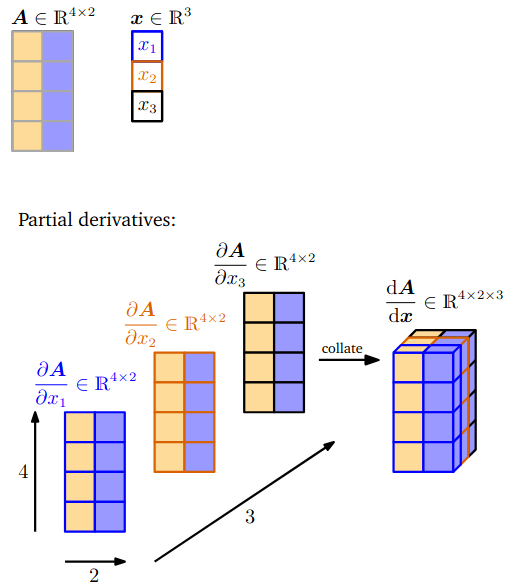
\includegraphics[
        width=\linewidth,
        height=5cm,
        keepaspectratio,
    ]{images/Vector-Calculus/Gradients-of-Matrices-approach1.png}
    \caption*{
        \textbf{Approach 1}: 
        We compute the partial derivative 
        $\dfrac{\partial \bm{A}}{\partial x_1}$ , 
        $\dfrac{\partial \bm{A}}{\partial x_2}$ , 
        $\dfrac{\partial \bm{A}}{\partial x_3}$ , each of which is a $4 \times 2$ matrix, 
        and collate them in a $4 \times 2 \times 3$ tensor.
        \cite{mfml/book/mml/Deisenroth-Faisal-Ong}
    }
\end{figure}
\end{minipage}
\hfill
\begin{minipage}{0.45\linewidth}
\begin{figure}[H]
    \centering
    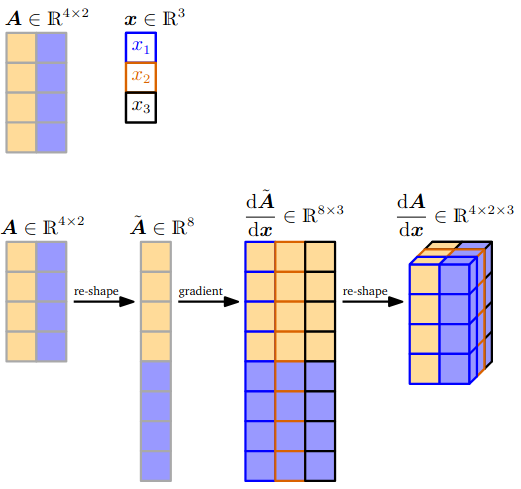
\includegraphics[
        width=\linewidth,
        height=5cm,
        keepaspectratio,
    ]{images/Vector-Calculus/Gradients-of-Matrices-approach2.png}
    \caption*{
        \textbf{Approach 2}: We re-shape (flatten) $\bm{A} \in \mbbR^{4\times 2}$ into a vector $\tilde{\bm{A}} \in \mbbR^8$. 
        Then, we compute the gradient $\dfrac{d\tilde{\bm{A}}}{d\bm{x}} \in \mbbR^{8\times 3}$. 
        We obtain the gradient tensor by re-shaping this gradient as illustrated above.
        \cite{mfml/book/mml/Deisenroth-Faisal-Ong}
    }
\end{figure}
\end{minipage}
\hfill
\end{table}


\begin{enumerate}
    \item 
    \begin{definition}[Tensor]
        Tensor is a multidimensional array
        \hfill \cite{mfml/book/mml/Deisenroth-Faisal-Ong}
    \end{definition}

    \item 
    \begin{definition}[Flattening (matrix $\to$ vector)]
        Matrices can be transformed into vectors by stacking the columns of the matrix
        \hfill \cite{mfml/book/mml/Deisenroth-Faisal-Ong}
    \end{definition}

    \item if we compute the gradient of an $m \times  n$ matrix $\bm{A}$ with respect to a $p \times  q$ matrix $\bm{B}$, the resulting Jacobian would be $(m\times n)\times (p\times q)$, i.e., a four-dimensional tensor $\bm{J}$, whose entries are given as $J_{ijkl} = \dfrac{\partial A_{ij}}{\partial B_{kl}}$.
    \hfill \cite{mfml/book/mml/Deisenroth-Faisal-Ong}
\end{enumerate}










\section{Differentiation Rules}

\begin{enumerate}[series=vcalrules]
    \item \textbf{Product rule}: 
    \begin{enumerate}
        \item $
            (f(x)g(x))^\prime
            = \dfrac{d}{dx}(f(x)g(x))
            = g(x)\dfrac{d}{dx}f(x) + f(x)\dfrac{d}{dx}g(x)
            = f^\prime(x)g(x) + f(x)g^\prime(x)
        $
        \hfill \cite{mfml/book/mml/Deisenroth-Faisal-Ong}

        \item $
            \dfrac{\partial}{\partial \bm{x}}(f(\bm{x})g(\bm{x}))
            = g(\bm{x})\dfrac{\partial}{\partial \bm{x}}f(\bm{x}) 
                + f(\bm{x})\dfrac{\partial}{\partial \bm{x}}g(\bm{x})
        $ \hfill \cite{mfml/book/mml/Deisenroth-Faisal-Ong}
    \end{enumerate}

    \item \textbf{Quotient rule}:
    $
        \dParenBrac{\dfrac{f(x)}{g(x)}}^\prime
        = \dfrac{d}{dx}\dParenBrac{\dfrac{f(x)}{g(x)}}
        = \dfrac{f^\prime(x)g(x) - f(x)g^\prime(x)}{(g(x))^2}
    $
    \hfill \cite{mfml/book/mml/Deisenroth-Faisal-Ong}

    \item \textbf{Sum Rule}:
    \begin{enumerate}
        \item $
            (f(x) + g(x))^\prime
            = f^\prime(x) + g^\prime(x)
        $
        \hfill \cite{mfml/book/mml/Deisenroth-Faisal-Ong}

        \item $
            \dfrac{\partial}{\partial \bm{x}}(f(\bm{x}) + g(\bm{x}))
            = \dfrac{\partial}{\partial \bm{x}}f(\bm{x}) 
                + \dfrac{\partial}{\partial \bm{x}}g(\bm{x})
        $
        \hfill \cite{mfml/book/mml/Deisenroth-Faisal-Ong}
    \end{enumerate}

    \item \textbf{Chain Rule}: 
    \begin{enumerate}
        \item $
            (g(f(x)))^\prime
            = (g \circ f)^\prime(x)
            = g^\prime(f(x)) f^\prime(x)
        $
        \hfill \cite{mfml/book/mml/Deisenroth-Faisal-Ong}

        \item $
            \dfrac{\partial}{\partial \bm{x}}(g(f(\bm{x})))
            = \dfrac{\partial}{\partial \bm{x}}(g \circ f)(\bm{x})
            = \dfrac{\partial g(\bm{x})}{\partial f(\bm{x})}
                \dfrac{\partial f(\bm{x})}{\partial \bm{x}}
        $
        \hfill \cite{mfml/book/mml/Deisenroth-Faisal-Ong}
    \end{enumerate}
    $g \circ f$ denotes function composition $x \mapsto f (x) \mapsto g(f (x))$.
    \hfill \cite{mfml/book/mml/Deisenroth-Faisal-Ong}
\end{enumerate}

\vspace{0.5cm}
\textbf{Gradients of Matrices \& Vectors}:

\begin{multicols}{2}
\begin{enumerate}[resume*=vcalrules]
    \item $
        \dfrac{\partial \bm{f}(\bm{A})^\top}{\partial \bm{A}}
        = \dParenBrac{\dfrac{\partial \bm{f}(\bm{A})}{\partial \bm{A}}}^\top
    $
    \hfill \cite{mfml/book/mml/Deisenroth-Faisal-Ong}

    \item $
        \dfrac{\partial\ \tr(\bm{f}(\bm{A}))}{\partial \bm{A}}
        = \tr\dParenBrac{\dfrac{\partial \bm{f}(\bm{A})}{\partial \bm{A}}}
    $
    \hfill \cite{mfml/book/mml/Deisenroth-Faisal-Ong}

    \item 
    $
        \dfrac{\partial \bm{f}(\bm{A})^{-1}}{\partial \bm{A}}
        = -\bm{f}(\bm{A})^{-1}\ \dfrac{\partial \bm{f}(\bm{A})}{\partial \bm{A}} \ \bm{f}(\bm{A})^{-1}
    $ 
    \hfill \cite{mfml/book/mml/Deisenroth-Faisal-Ong}

    \item 
    $
        \dfrac{\partial\ \bm{x}^\top \bm{A}^{-1}\bm{y}}{\partial \bm{A}}
        = -(\bm{A}^{-1})^\top \bm{xy}^\top (\bm{A}^{-1})^\top
    $
    \hfill \cite{mfml/book/mml/Deisenroth-Faisal-Ong}

    \item 
    $
        \dfrac{\partial\ \bm{x}^\top \bm{A}\bm{y}}{\partial \bm{A}}
        = \bm{xy}^\top 
    $
    \hfill \cite{mfml/book/mml/Deisenroth-Faisal-Ong}

    \item 
    $
        \dfrac{\partial\ \bm{x}^\top \bm{A}\bm{x}}{\partial \bm{x}}
        = \bm{x}^\top(\bm{A} + \bm{A}^\top) 
    $
    \hfill \cite{mfml/book/mml/Deisenroth-Faisal-Ong}

    \item 
    $
        \dfrac{\partial\ \bm{x}^\top \bm{y}}{\partial\ \bm{x}} = \bm{y}^\top
    $
    \hfill \cite{mfml/book/mml/Deisenroth-Faisal-Ong}

    \item 
    $
        \dfrac{\partial\ \bm{y}^\top \bm{x}}{\partial\ \bm{x}} = \bm{y}^\top
    $
    \hfill \cite{mfml/book/mml/Deisenroth-Faisal-Ong}
\end{enumerate}
\end{multicols}

\vspace{0.5cm}
\begin{enumerate}[resume*=vcalrules]
    \item $
        \dfrac{\partial \det(\bm{f}(\bm{A}))}{\partial \bm{A}}
        = \det(\bm{f}(\bm{A}))\ \tr\dParenBrac{\bm{f}(\bm{A})^{-1}\ \dfrac{\partial \bm{f}(\bm{A})}{\partial \bm{A}}}
    $
    \hfill \cite{mfml/book/mml/Deisenroth-Faisal-Ong}

    \item 
    $
        \dfrac{\partial\ (\bm{x} - \bm{As})^\top \bm{W} (\bm{x} - \bm{As})}{\partial\bm{s}}
        = -2(\bm{x} - \bm{As})^\top \bm{WA}
    $
    \hfill
    (for symmetric $\bm{W}$)
    \hfill \cite{mfml/book/mml/Deisenroth-Faisal-Ong}
\end{enumerate}


\vspace{0.5cm}
\textbf{Examples}
\begin{enumerate}
    \item Consider a function $f : \mbbR^2 \to \mbbR$ of two variables $x_1, x_2$. 
    Furthermore, $x_1(t)$ and $x_2(t)$ are themselves functions of $t$. 
    \\
    $
        \nabla_t f(x_1, x_2)
        = \dfrac{df}{dt}
        = \begin{bmatrix}
            \dfrac{\partial f(x_1, x_2)}{\partial x_1(t)} &
            \dfrac{\partial f(x_1, x_2)}{\partial x_2(t)}
        \end{bmatrix}
        \begin{bmatrix}
            \dfrac{\partial x_1(t)}{\partial t} \\
            \dfrac{\partial x_2(t)}{\partial t}
        \end{bmatrix}
        = \dfrac{\partial f(x_1, x_2)}{\partial x_1(t)} \dfrac{\partial x_1(t)}{\partial t}
        + \dfrac{\partial f(x_1, x_2)}{\partial x_2(t)} \dfrac{\partial x_2(t)}{\partial t}
    $
    \hfill \cite{mfml/book/mml/Deisenroth-Faisal-Ong}

    \item If $f (x_1, x_2)$ is a function of $x_1$ and $x_2$, where $x_1(s, t)$ and $x_2(s, t)$ are themselves functions of two variables $s$ and $t$:
    \\
    $
        \begin{aligned}
        \nabla_{(s,t)} f(x_1, x_2)
        &= \dfrac{df(x_1, x_2)}{d(s,t)}
        = \dfrac{\partial f}{\partial \bm{x}} \dfrac{\partial \bm{x}}{\partial (s,t)}
        = \begin{bmatrix}
            \dfrac{\partial f(x_1, x_2)}{\textcolor{blue}{\partial x_1(s,t)}} &
            \dfrac{\partial f(x_1, x_2)}{\textcolor{green}{\partial x_2(s,t)}}
        \end{bmatrix}
        \begin{bmatrix}
            \textcolor{blue}{\dfrac{\partial x_1(s,t)}{\partial s}} & \textcolor{blue}{\dfrac{\partial x_1(s,t)}{\partial t}} \\
            \textcolor{green}{\dfrac{\partial x_2(s,t)}{\partial s}} & \textcolor{green}{\dfrac{\partial x_2(s,t)}{\partial t}}
        \end{bmatrix}
        \\
        &= 
        \begin{bmatrix}
            \dfrac{\partial f(x_1, x_2)}{\textcolor{blue}{\partial x_1(s,t)}}
            \textcolor{blue}{\dfrac{\partial x_1(s,t)}{\partial s}} +
            \dfrac{\partial f(x_1, x_2)}{\textcolor{green}{\partial x_2(s,t)}}
            \textcolor{green}{\dfrac{\partial x_2(s,t)}{\partial s}} \\ 
            \dfrac{\partial f(x_1, x_2)}{\textcolor{blue}{\partial x_1(s,t)}}
            \textcolor{blue}{\dfrac{\partial x_1(s,t)}{\partial t}} +
            \dfrac{\partial f(x_1, x_2)}{\textcolor{green}{\partial x_2(s,t)}}
            \textcolor{green}{\dfrac{\partial x_2(s,t)}{\partial t}}
        \end{bmatrix}
        \end{aligned}
    $
    \hfill \cite{mfml/book/mml/Deisenroth-Faisal-Ong}
    
\end{enumerate}




















\section{Backpropagation: Gradients in DNN}

\begin{table}[H]
\begin{minipage}{0.48\linewidth}
    \begin{figure}[H]
        \centering
        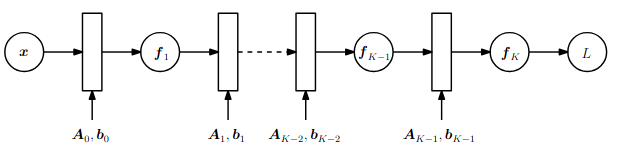
\includegraphics[
            width=\linewidth,
            height=3cm,
            keepaspectratio,
        ]{images/Vector-Calculus/sample-dnn-bp-ad.png}
        \caption*{
            Forward pass in a multi-layer neural network to compute the loss $L$ as a function of the inputs $\bm{x}$ and the parameters $\bm{A}_i, \bm{b}_i$.
            \cite{mfml/book/mml/Deisenroth-Faisal-Ong}
        }
    \end{figure}
\end{minipage}
\hfill
\vline
\hfill
\begin{minipage}{0.48\linewidth}
    \begin{figure}[H]
        \centering
        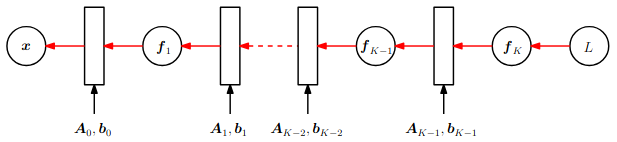
\includegraphics[
            width=\linewidth,
            height=3cm,
            keepaspectratio,
        ]{images/Vector-Calculus/sample-dnn-bp-ad2.png}
        \caption*{
            Backward pass in a multi-layer neural network to compute the gradients of the loss function.
            \cite{mfml/book/mml/Deisenroth-Faisal-Ong}
        }
    \end{figure}
\end{minipage}
\end{table}

\begin{enumerate}
    \item An area where the chain rule is used to an extreme is deep learning, where the function value $\bm{y}$ is computed as a many-level function composition 
    \hfill \cite{mfml/book/mml/Deisenroth-Faisal-Ong}
    \\
    .\hfill
    $
        \bm{y}
        = (f_K \circ f_{K-1} \circ \cdots \circ f_1)(\bm{x})
        = f_K (f_{K-1}(\cdots (f_1(\bm{x}))\cdots))
    $
    \hfill \cite{mfml/book/mml/Deisenroth-Faisal-Ong}
    \\
    where $\bm{x}$ are the inputs (e.g., images), $\bm{y}$ are the observations (e.g., class labels), and every function $f_i, i = 1, \cdots , K$, possesses its own parameters.
    \hfill \cite{mfml/book/mml/Deisenroth-Faisal-Ong}
    \\
    \begin{multicols}{2}
    \begin{enumerate}[series=grad-dnn]
        \item $\bm{f}_0 := \bm{x}$
        \hfill \cite{mfml/book/mml/Deisenroth-Faisal-Ong}

        \item $\bm{f}_i := \sigma_i(\bm{A}_{i-1}\bm{f}_{i-1} + \bm{b}_{i-1})$
        \hfill \cite{mfml/book/mml/Deisenroth-Faisal-Ong}

        \item $\bm{f}_i(\bm{x}_{i-1}) = \sigma_i(\bm{A}_{i-1}\bm{x}_{i-1} + \bm{b}_{i-1})$
        \hfill \cite{mfml/book/mml/Deisenroth-Faisal-Ong}

        \item $\bm{y} = \bm{f}_K(\bm{x}_{K-1})$
        \hfill \cite{mfml/book/mml/Deisenroth-Faisal-Ong}
    \end{enumerate}
    \end{multicols}
    \begin{multicols}{2}
    \begin{enumerate}[resume*=grad-dnn]
        \item $L(\bm{\theta}) = \dnorm{\bm{y} - \bm{f}_K(\bm{\theta},\ \bm{x})}^2$
        \hfill \cite{mfml/book/mml/Deisenroth-Faisal-Ong}
        
        \item 
        $
            \dfrac{\partial L}{\partial \bm{\theta}_{K-1}}
            = \dfrac{\partial L}{\partial \bm{f}_K} \textcolor{blue}{\dfrac{\partial \bm{f}_K}{\partial \bm{\theta}_{K-1}}}
        $
        \hfill \cite{mfml/book/mml/Deisenroth-Faisal-Ong}

        \item 
        $
            \dfrac{\partial L}{\partial \bm{\theta}_{K-2}}
            = \dfrac{\partial L}{\partial \bm{f}_K} 
            \textcolor{orange}{\dfrac{\partial \bm{f}_K}{\partial \bm{\theta}_{K-1}}}
            \textcolor{blue}{\dfrac{\partial \bm{f}_{K-1}}{\partial \bm{\theta}_{K-2}}}
        $
        \hfill \cite{mfml/book/mml/Deisenroth-Faisal-Ong}

        \item 
        $
            \dfrac{\partial L}{\partial \bm{\theta}_{K-2}}
            = \dfrac{\partial L}{\partial \bm{f}_K} 
            \textcolor{orange}{
                \dfrac{\partial \bm{f}_K}{\partial \bm{\theta}_{K-1}} 
                \cdots
                \dfrac{\partial \bm{f}_{i+2}}{\partial \bm{\theta}_{i+1}} 
            }
            \textcolor{blue}{\dfrac{\partial \bm{f}_{i+1}}{\partial \bm{\theta}_{i}}}
        $
        \hfill \cite{mfml/book/mml/Deisenroth-Faisal-Ong}
    \end{enumerate}
    \end{multicols}
    \begin{enumerate}
        \item [\textcolor{orange}{orange}] partial derivatives of the output of a layer with respect to its inputs

        \item [\textcolor{blue}{blue}] partial derivatives of the output of a layer with respect to its parameters
    \end{enumerate}
    \vspace{0.5cm}
    \textbf{where}:
    \begin{multicols}{2}
    \begin{enumerate}
        \item $i$: layer ($i = 1,\cdots,K$)
        \hfill \cite{mfml/book/mml/Deisenroth-Faisal-Ong}
        
        \item $\bm{x}_{i-1}$: output of layer $i - 1$
        \hfill \cite{mfml/book/mml/Deisenroth-Faisal-Ong}
        
        \item $\sigma_i$: activation function of layer $i$
        \hfill \cite{mfml/book/mml/Deisenroth-Faisal-Ong}

        \item $L$: loss function
        \hfill \cite{mfml/book/mml/Deisenroth-Faisal-Ong}

        \item $\bm{A}_{j},\ \bm{b}_{j}$: parameters ($j = 0,\cdots,K-1$)
        \hfill \cite{mfml/book/mml/Deisenroth-Faisal-Ong}

        \item $\bm{\theta} = \dCurlyBrac{\bm{A}_{0},\ \bm{b}_{0}, \cdots, \bm{A}_{K-1},\ \bm{b}_{K-1}}$
        \hfill \cite{mfml/book/mml/Deisenroth-Faisal-Ong}
    \end{enumerate}
    \end{multicols}

\end{enumerate}








\section{Computational Graph}

\begin{enumerate}
    \item 
    \begin{definition}[Computational Graph]
        Computational graphs are a type of graph that can be used to represent mathematical expressions. 
        This is similar to descriptive language in the case of deep learning models, providing a functional description of the required computation.
        \hfill \cite{geeksforgeeks/deep-learning/computational-graphs-in-deep-learning}
    \end{definition}

    \item In general, the computational graph is a \textbf{directed graph} that is used for expressing and evaluating mathematical expressions. 
    \hfill \cite{geeksforgeeks/deep-learning/computational-graphs-in-deep-learning}

    \item These can be used for two different types of calculations:
    \hfill \cite{geeksforgeeks/deep-learning/computational-graphs-in-deep-learning}
    \begin{enumerate}
        \item Forward computation
        \hfill \cite{geeksforgeeks/deep-learning/computational-graphs-in-deep-learning}
        
        \item Backward computation
        \hfill \cite{geeksforgeeks/deep-learning/computational-graphs-in-deep-learning}
    \end{enumerate}

    \item Structure of a computational graph:
    \begin{enumerate}
        \item A variable is represented by a \textbf{node} in a graph. 
        It could be a scalar, vector, matrix, tensor, or even another type of variable.
        \hfill \cite{geeksforgeeks/deep-learning/computational-graphs-in-deep-learning}
    
        \item A function argument and data dependency are both represented by an \textbf{edge}. 
        These are similar to node pointers.
        \hfill \cite{geeksforgeeks/deep-learning/computational-graphs-in-deep-learning}
    
        \item A simple function of one or more variables is called an operation. 
        There is a set of operations that are permitted. 
        Functions that are more complex than these operations in this set can be represented by combining multiple operations.
        \hfill \cite{geeksforgeeks/deep-learning/computational-graphs-in-deep-learning}
    \end{enumerate}

    \item Types of computational graphs:
    \begin{enumerate}
        \item Static Computational Graphs
        \hfill \cite{geeksforgeeks/deep-learning/computational-graphs-in-deep-learning}

        \item Dynamic Computational Graphs
        \hfill \cite{geeksforgeeks/deep-learning/computational-graphs-in-deep-learning}
    \end{enumerate}
\end{enumerate}


\subsection{Static Computational Graphs}
\begin{enumerate}
    \item Involves two phases
    \begin{enumerate}
        \item Phase 1:- Make a plan for your architecture
        \hfill \cite{geeksforgeeks/deep-learning/computational-graphs-in-deep-learning}

        \item Phase 2:- To train the model and generate predictions, feed it a lot of data.
        \hfill \cite{geeksforgeeks/deep-learning/computational-graphs-in-deep-learning}
    \end{enumerate}

    \item The benefit of utilizing this graph is that it enables powerful offline graph optimization and scheduling. As a result, they should be faster than dynamic graphs in general.
    \hfill \cite{geeksforgeeks/deep-learning/computational-graphs-in-deep-learning}

    \item The drawback is that dealing with structured and even variable-sized data is unsightly.
    \hfill \cite{geeksforgeeks/deep-learning/computational-graphs-in-deep-learning}
\end{enumerate}



\subsection{Dynamic Computational Graphs}

\begin{enumerate}
    \item As the forward computation is performed, the graph is implicitly defined.
    
    \item This graph has the advantage of being more adaptable. 
    The library is less intrusive and enables interleaved graph generation and evaluation. 
    The forward computation is implemented in your preferred programming language, complete with all of its features and algorithms. 
    Debugging dynamic graphs is simple because it permits line-by-line execution of the code and access to all variables, finding bugs in your code is considerably easier. 
    
    \item The disadvantage of employing this graph is that there is limited time for graph optimization, and the effort may be wasted if the graph does not change.
\end{enumerate}






\section{Automatic Differentiation}

\begin{enumerate}
    \item[] \textbf{Example}: $x \mapsto a \mapsto b \mapsto y$
    \hspace{1cm}
    $
        \dfrac{dy}{dx} = \dfrac{dy}{db}\ \dfrac{db}{da}\ \dfrac{da}{dx}
    $
    \hfill \cite{mfml/book/mml/Deisenroth-Faisal-Ong}

    \item 
    \begin{definition}[Automatic differentiation]
        Automatic differentiation is different from symbolic differentiation and numerical approximations of the gradient, e.g., by using finite differences.
        We can think of automatic differentiation as a set of techniques to numerically (in contrast to symbolically) evaluate the exact (up to machine precision) gradient of a function by working with intermediate variables and applying the chain rule.
        \hfill \cite{mfml/book/mml/Deisenroth-Faisal-Ong}
    \end{definition}


    \item Automatic differentiation applies a series of elementary arithmetic operations, e.g., addition and multiplication and elementary functions, e.g., sin, cos, exp, log. 
    \hfill \cite{mfml/book/mml/Deisenroth-Faisal-Ong}
    
    \item By applying the chain rule to these operations, the gradient of quite complicated functions can be computed automatically.
    \hfill \cite{mfml/book/mml/Deisenroth-Faisal-Ong}

    \item Automatic differentiation applies to general computer programs and has forward and reverse modes.
    Intuitively, the forward and reverse mode differ in the order of multiplication.
    \\
    $\dfrac{dy}{dx} = \dParenBrac{\dfrac{dy}{db}\ \dfrac{db}{da}}\ \dfrac{da}{dx}$ would be the reverse mode because gradients are propagated backward through the graph, i.e., reverse to the data flow.
    $\dfrac{dy}{dx} = \dfrac{dy}{db}\ \dParenBrac{\dfrac{db}{da}\ \dfrac{da}{dx}}$ would be the forward mode, where the gradients flow with the data from left to right through the graph.
    
    \item In the context of neural networks, where the input dimensionality is often much higher than the dimensionality of the labels, the reverse mode is computationally significantly cheaper than the forward mode.
    \hfill \cite{mfml/book/mml/Deisenroth-Faisal-Ong}

    \item Let $x_1, \cdots , x_d$ be the input variables to the function, $x_{d+1}, \cdots , x_{D-1}$ be the intermediate variables, and $x_D$ the output variable. Then the computation graph can be expressed as follows:
    \hfill \cite{mfml/book/mml/Deisenroth-Faisal-Ong}
    \\
    \textbf{Forward propagation}:\hfill
    $x_i = g_i(x_{Pa(x_i)})$ 
    \hspace{1cm} 
    $i = d+1, \cdots, D$
    \hspace{1cm} 
    $f = x_D$
    \hfill \cite{mfml/book/mml/Deisenroth-Faisal-Ong}
    \\
    where 
    $g_i(\cdot)$ are elementary functions 
    $Pa(x_i)$ are indices (ex: $Pa(x_0) = \dCurlyBrac{1, 2}$) of parent nodes of the variable $x_i$ in the graph
    and 
    $x_{Pa(x_i)}$ are the parent nodes (ex: $x_{Pa(x_0)} = \dCurlyBrac{x_1, x_2}$) of the variable $x_i$ in the graph.
    \hfill \cite{mfml/book/mml/Deisenroth-Faisal-Ong}
    \\
    \textbf{Backward propagation}:\hfill
    $\dfrac{\partial f}{\partial x_D} = 1$
    \hspace{1cm}
    $
        \dfrac{\partial f}{\partial x_i}
        = \dsum_{j; i \in Pa(x_j)} \dfrac{\partial f}{\partial x_j} \dfrac{\partial x_j}{\partial x_i}
        = \dsum_{j; i \in Pa(x_j)} \dfrac{\partial f}{\partial x_j} \dfrac{\partial g_j}{\partial x_i}
    $
    \hfill \cite{mfml/book/mml/Deisenroth-Faisal-Ong}


    \item The automatic differentiation approach above works whenever we have a function that can be expressed as a computation graph, where the elementary functions are differentiable. 
    In fact, the function may not even be a mathematical function but a computer program. 
    However, not all computer programs can be automatically differentiated, e.g., if we cannot find differential elementary functions. 
    Programming structures, such as \verb|for| loops and \verb|if| statements, require more care as well.
    \hfill \cite{mfml/book/mml/Deisenroth-Faisal-Ong}







    \item \textbf{Example}: $f(x) = \sqrt{x^2 + \exp(x^2)} + \cos\dParenBrac{x^2 + \exp(x^2)}$
    \begin{figure}[H]
        \centering
        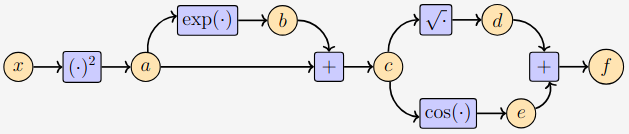
\includegraphics[
            width=\linewidth,
            height=2cm,
            keepaspectratio,
        ]{images/Vector-Calculus/example-auto-diff-comp-graph.png}
        \caption*{
            Computation graph with inputs $x$, function values $f$, and intermediate variables $a, b, c, d, e$.
            \cite{mfml/book/mml/Deisenroth-Faisal-Ong}
        }
    \end{figure}
    \begin{multicols}{6}
    \begin{enumerate}[leftmargin=0.1cm, label={}]
        \item[] $a = x^2$
        \item[] $b = \exp(a)$
        \item[] $c = a+b$
        \item[] $d = \sqrt{c}$
        \item[] $e = \cos(c)$
        \item[] $f = d+e$
    \end{enumerate}
    \end{multicols}
    \begin{multicols}{6}
    \begin{enumerate}[leftmargin=0.1cm, label={}]
        \item[] $\dfrac{\partial a}{\partial x} = 2x$
        \item[] $\dfrac{\partial b}{\partial a} = \exp(a)$
        \item[] $\dfrac{\partial c}{\partial a} = \dfrac{\partial c}{\partial b} = 1$
        \item[] $\dfrac{\partial d}{\partial c} = \dfrac{1}{2\sqrt{c}}$
        \item[] $\dfrac{\partial e}{\partial c} = -\sin(c)$
        \item[] $\dfrac{\partial f}{\partial d} = \dfrac{\partial f}{\partial e} = 1$
    \end{enumerate}
    \end{multicols}
    \begin{multicols}{3}
    \begin{enumerate}[leftmargin=0.1cm, label={}]
        \item[] $
            \dfrac{\partial f}{\partial c}
            = \dfrac{\partial f}{\partial d} \dfrac{\partial d}{\partial c}
            + \dfrac{\partial f}{\partial e} \dfrac{\partial e}{\partial c}
        $
        \item[] $
            \dfrac{\partial f}{\partial a}
            = \dfrac{\partial f}{\partial b} \dfrac{\partial b}{\partial a}
            + \dfrac{\partial f}{\partial c} \dfrac{\partial c}{\partial a}
        $
        \item[] 
        $
            \dfrac{\partial f}{\partial b}
            = \dfrac{\partial f}{\partial c} \dfrac{\partial c}{\partial b}
        $
            \hspace{0.2cm}
            \vline
            \hspace{0.2cm}
        $
            \dfrac{\partial f}{\partial x}
            = \dfrac{\partial f}{\partial a} \dfrac{\partial a}{\partial x}
        $
    \end{enumerate}
    \end{multicols}
\end{enumerate}


























\chapter{Systems of Linear Equations}

% \begin{enumerate}
%     \item \textbf{Algebra} is constructing a set of objects (symbols) and a set of rules to manipulate these objects.
%     \hfill \cite{mfml/book/mml/Deisenroth-Faisal-Ong}

%     \item \textbf{Linear algebra} is the study of vectors and certain rules to manipulate vectors.
%     \hfill \cite{mfml/book/mml/Deisenroth-Faisal-Ong}
% \end{enumerate}


\begin{customArrayStretch}{1.3}
\begin{table}[H]
    \centering
    \begin{tabular}{| l | l  l |}
        \hline

        coefficients & $a_{ij}$    & $\in \mbbR$ \\ \hline

        constants & $b_{i}$     & $\in \mbbR$ \\ \hline

        unknowns & $x_{i}$     & $\in \mbbR$ \\ \hline

    \end{tabular}
    \caption*{Notations}
\end{table}
\end{customArrayStretch}


\vspace{0.5cm}


\begin{enumerate}
    \item \textbf{general form} of a system of linear equations:
    \\
    .\hfill
    $
        \begin{aligned}
            a_{11}x_1\  & +\ & \cdots\ & +\ & a_{1n}x_n\ & =\ & b_1 \\
            & & & \vdots \\
            a_{m1}x_1\  & +\ & \cdots\ & +\ & a_{mn}x_n\ & =\ & b_m
        \end{aligned}
    $
    \hfill \cite{mfml/book/mml/Deisenroth-Faisal-Ong}
    \vspace{0.2cm}
    \begin{enumerate}
        \item $x_1, \cdots , x_n$ are the \textbf{unknowns} of this system.

        \item Every $n$-tuple $(x_1, \cdots , x_n) \in \mbbR^n$ that satisfies this system is a \textbf{solution} of the linear equation system.
    \end{enumerate}


    \item \textbf{compact notation}:
    \\[0.2cm]
    $
        \begin{bmatrix}a_{11}\\ \vdots\\ a_{m1}\end{bmatrix} \bm{x}_1 +
        \begin{bmatrix}a_{12}\\ \vdots\\ a_{m2}\end{bmatrix} \bm{x}_2 +
        \cdots +
        \begin{bmatrix}a_{1n}\\ \vdots\\ a_{mn}\end{bmatrix} \bm{x}_n =
        \begin{bmatrix}b_{1}\\ \vdots\\ b_{m}\end{bmatrix}
    \Longleftrightarrow
        \underset{\displaystyle\bm{A}}{\underbrace{\begin{bmatrix}
            a_{11} & \cdots & a_{1n} \\
            \vdots & \ddots & \vdots \\
            a_{m1} & \cdots & a_{mn}
        \end{bmatrix}}} \
        \underset{\displaystyle\bm{x}}{\underbrace{\begin{bmatrix} x_{1} \\ \vdots \\ x_{n} \end{bmatrix}}}
        =
        \underset{\displaystyle\bm{b}}{\underbrace{\begin{bmatrix} b_{1} \\ \vdots \\ b_{m} \end{bmatrix}}}
    $
    \hfill \cite{mfml/book/mml/Deisenroth-Faisal-Ong}



\end{enumerate}


\vspace{0.5cm}
\textbf{Note}:
\begin{enumerate}
    \item In general, for a real-valued system of linear equations we obtain either no, exactly one, or infinitely many solutions.
    \hfill \cite{mfml/book/mml/Deisenroth-Faisal-Ong}

    \item \textbf{Geometric Interpretation of Systems of Linear Equations}:
    In a system of linear equations with two variables $x_1$, $x_2$, each linear equation defines a line on the $x_1x_2$-plane. Since a solution to a system of linear equations must satisfy all equations simultaneously, the solution set is the intersection of these lines. This intersection set can be a line (if the linear equations describe the same line), a point, or empty (when the lines are parallel).
    \hfill \cite{mfml/book/mml/Deisenroth-Faisal-Ong}
    \\
    Similarly, for three variables, each linear equation determines a plane in three-dimensional space. When we intersect these planes, i.e., satisfy all linear equations at the same time, we can obtain a solution set that is a plane, a line, a point or empty (when the planes have no common intersection).
    \hfill \cite{mfml/book/mml/Deisenroth-Faisal-Ong}

    \item the product $Ax$ is a (linear) combination of the columns of $A$
    \hfill \cite{mfml/book/mml/Deisenroth-Faisal-Ong}

    \item \textbf{Augmented Matrix} ( $\dSquareBrac{\bm{A}|\bm{b}}$ ):
    \\[0.2cm]
    $
        \left[
        \begin{array}{ccc|c}
            a_{11} & \cdots & a_{1n} & b_{1}\\
            \vdots & \ddots & \vdots & \vdots \\
            a_{m1} & \cdots & a_{mn} & b_{m}
        \end{array}
        \right]
    $

    \item The solution set of a homogeneous system of linear equations $\bm{Ax} = \bm{0}$ with $n$ unknowns $\bm{x} = [x_1, \cdots , x_n]^\top$ is a subspace of $\mbbR^n$.
    \hfill \cite{mfml/book/mml/Deisenroth-Faisal-Ong}

    \item Every subspace $U \subseteq (\mbbR^n , +, \cdot)$ is the solution space of a homogeneous system of linear equations $\bm{Ax} = \bm{0}$ for $\bm{x} \in \mbbR^n$.
    \hfill \cite{mfml/book/mml/Deisenroth-Faisal-Ong}

    \item The solution of an inhomogeneous system of linear equations $\bm{Ax} = \bm{b}, \bm{b} \neq \bm{0}$ is not a subspace of $\mbbR^n$.
    \hfill \cite{mfml/book/mml/Deisenroth-Faisal-Ong}


\end{enumerate}








\section{Types of Solutions}

\begin{enumerate}

\item \textbf{Unique Solution}:
\begin{enumerate}
    \item The system has exactly one solution.
    \hfill \cite{common/online/chatgpt}

    \item \textbf{Graphically}: The lines (or planes) intersect at a single point.
    \hfill \cite{common/online/chatgpt}

    \item \textbf{Algebraically}: The equations are independent and consistent.
    \hfill \cite{common/online/chatgpt}
\end{enumerate}

\item \textbf{Infinite Solutions}:
\begin{enumerate}
    \item The system has infinitely many solutions.
    \hfill \cite{common/online/chatgpt}

    \item \textbf{Graphically}: The lines (or planes) are exactly the same (i.e., they overlap).
    \hfill \cite{common/online/chatgpt}

    \item \textbf{Algebraically}: The equations are dependent and consistent.
    \hfill \cite{common/online/chatgpt}
\end{enumerate}

\item \textbf{No Solution}:
\begin{enumerate}
    \item The system has no common solution.
    \hfill \cite{common/online/chatgpt}

    \item \textbf{Graphically}: The lines are parallel (in 2D) and never meet.
    \hfill \cite{common/online/chatgpt}

    \item \textbf{Algebraically}: The system is inconsistent.
    \hfill \cite{common/online/chatgpt}
\end{enumerate}

\end{enumerate}


\section{Finding Solutions using Matrix Inverse}

\begin{enumerate}
    \item if $\bm{A}$ is a square matrix and invertible (strict conditions): $\bm{x} = \bm{A}^{-1}\bm{b}$
    \hfill \cite{mfml/book/mml/Deisenroth-Faisal-Ong}

    \item if $\bm{A}$ has linearly independent columns (mild assumptions): $\bm{x} = (\bm{A}^\top  \bm{A})^{-1}\bm{A}^\top \bm{b}$
    \hfill \cite{mfml/book/mml/Deisenroth-Faisal-Ong}

    \item for reasons of numerical precision it is generally not recommended to compute the inverse or pseudo-inverse
    \hfill \cite{mfml/book/mml/Deisenroth-Faisal-Ong}
\end{enumerate}


\section{Finding Solutions using Elementary Transformations}

\begin{enumerate}
    \item keep the solution set the same, but that transform the equation system into a simpler form
    \hfill \cite{mfml/book/mml/Deisenroth-Faisal-Ong}

    \item Operations:
    \begin{enumerate}
        \item Exchange of two equations (rows in the matrix representing the system of equations)
        \hfill \cite{mfml/book/mml/Deisenroth-Faisal-Ong}

        \item Multiplication of an equation (row) with a constant $\lambda \in \mbbR \backslash \dCurlyBrac{0}$
        \hfill \cite{mfml/book/mml/Deisenroth-Faisal-Ong}

        \item Addition of two equations (rows)
        \hfill \cite{mfml/book/mml/Deisenroth-Faisal-Ong}
    \end{enumerate}

    \item Disadvantages:
    \begin{enumerate}
        \item for systems with millions of variables, it is impractical as the required number of arithmetic operations scales cubically in the number of simultaneous equations.
        \hfill \cite{mfml/book/mml/Deisenroth-Faisal-Ong}
    \end{enumerate}
\end{enumerate}



\subsection{Row-Echelon Form (REF)}

\begin{enumerate}
    \item
    \begin{definition}[REF: pivot]
        The leading coefficient of a row (first nonzero number from the left) is called the pivot and is always strictly to the right of the pivot of the row above it.
        \hfill \cite{mfml/book/mml/Deisenroth-Faisal-Ong}
    \end{definition}

    \item any equation system in row-echelon form always has a “staircase” structure
    \hfill \cite{mfml/book/mml/Deisenroth-Faisal-Ong}

    \item A matrix is in row-echelon form if
    \begin{enumerate}
        \item All rows that contain only zeros are at the bottom of the matrix; correspondingly, all rows that contain at least one nonzero element are on top of rows that contain only zeros.
        \hfill \cite{mfml/book/mml/Deisenroth-Faisal-Ong}

        \item Looking at nonzero rows only, the first nonzero number from the left (also called the \textbf{pivot} or the \textbf{leading coefficient}) is always strictly to the right of the pivot of the row above it.
        \hfill \cite{mfml/book/mml/Deisenroth-Faisal-Ong}
    \end{enumerate}

    \item The variables corresponding to the pivots in the row-echelon form are called basic variables and the other variables are free variables.
    \hfill \cite{mfml/book/mml/Deisenroth-Faisal-Ong}

    \item we express the right-hand side of the equation system using the pivot columns, such that $\bm{b} = \dsum^P_{i=1} \lambda_i\ \bm{p}_i$, where $\bm{p}_i$ , $i = 1, \cdots , P$, are the pivot columns.
    \\
    The $\lambda_i$ are determined easiest if we start with the rightmost pivot column and work our way to the left.
    \hfill \cite{mfml/book/mml/Deisenroth-Faisal-Ong}


\end{enumerate}



\subsection{Reduced Row-Echelon Form (RREF)/ row-reduced echelon form/ row canonical form \cite{mfml/book/mml/Deisenroth-Faisal-Ong}}

\begin{enumerate}
    \item An equation system is in reduced reduced row-echelon form if:
    \begin{enumerate}
        \item It is in row-echelon form.
        \hfill \cite{mfml/book/mml/Deisenroth-Faisal-Ong}

        \item Every pivot is $1$.
        \hfill \cite{mfml/book/mml/Deisenroth-Faisal-Ong}

        \item The pivot is the only non-zero entry in its column.
        \hfill \cite{mfml/book/mml/Deisenroth-Faisal-Ong}
    \end{enumerate}

    \item Gaussian elimination is an algorithm that performs elementary transformations to bring a system of linear equations into reduced row-echelon form.
    \hfill \cite{mfml/book/mml/Deisenroth-Faisal-Ong}
\end{enumerate}



\subsection{Particular Solution/ Special solution}

\begin{customArrayStretch}{1.3}
\begin{table}[H]
    \centering
    \begin{tabular}{|l|l|l|}
        \hline
        \textbf{Term} &
            \textbf{Scope} &
            \textbf{Context} \\ \hline \hline

        \textbf{Unique Solution} &
            One and only one solution &
            Systems of equations \\ \hline

        \textbf{Particular Solution} &
            One of possibly many solutions &
            Differential equations, infinite solution systems \\ \hline

    \end{tabular}
    \caption*{Unique Solution VS Particular Solution \cite{common/online/chatgpt}}
\end{table}
\end{customArrayStretch}


\begin{enumerate}
    \item this is not the only solution of this system of linear equations.
    \hfill \cite{mfml/book/mml/Deisenroth-Faisal-Ong}

    \item To capture all the other solutions, we need to be creative in generating $0$ in a non-trivial way using the columns of the matrix: Adding $0$ to our special solution \textbf{does not} change the special solution.
    \hfill \cite{mfml/book/mml/Deisenroth-Faisal-Ong}


\end{enumerate}




\subsection{Finding Solutions to $Ax=0$: Minus-$1$ Trick \cite{mfml/book/mml/Deisenroth-Faisal-Ong}}

Let $\bm{A}$ is in reduced row-echelon form without any rows that just contain zeros:\\
.\hfill
$
    \bm{A}
    =
    \begin{bmatrix}
        0 & \cdots & 0 & \mathbf{1} & * & \cdots & * & 0 & * & \cdots & * & 0 & * & \cdots & * \\
        \vdots & & \vdots & 0 & 0 & \cdots & 0 & \mathbf{1} & * & \cdots & * & \vdots & \vdots & & \vdots\\
        \vdots & & \vdots & \vdots & \vdots &  & \vdots & 0 & \vdots & & \vdots & \vdots & \vdots & & \vdots\\
        \vdots & & \vdots & \vdots & \vdots &  & \vdots & \vdots & \vdots & & \vdots & 0 & \vdots & & \vdots\\
        0 & \cdots & 0 & 0 & 0 & \cdots & 0 & 0 & 0 & \cdots & 0 & \mathbf{1} & * & \cdots & *
    \end{bmatrix}
    \in \mbbR^{k\times n}
$
\hfill \cite{mfml/book/mml/Deisenroth-Faisal-Ong}

\vspace{0.2cm}

\begin{enumerate}
    \item $*$ can be an arbitrary real number
    \hfill \cite{mfml/book/mml/Deisenroth-Faisal-Ong}

    \item constraints:
    \begin{enumerate}
        \item first nonzero entry per row must be $1$
        \hfill \cite{mfml/book/mml/Deisenroth-Faisal-Ong}

        \item all other entries in the corresponding column must be $0$
        \hfill \cite{mfml/book/mml/Deisenroth-Faisal-Ong}
    \end{enumerate}

    \item The columns $j_1, \cdots , j_k$ with the pivots (marked in \textbf{bold}) are the standard unit vectors $e_1, \cdots , e_k \in \mbbR^k$.
    \hfill \cite{mfml/book/mml/Deisenroth-Faisal-Ong}

    \item We extend this matrix to an $n \times n$-matrix $\tilde{\bm{A}}$ by adding $n - k$ rows of the form
    $
        \begin{bmatrix}
            0 & \cdots & 0 & -1 & 0 & \cdots & 0
        \end{bmatrix}
    $
    so that the diagonal of the augmented matrix $\tilde{\bm{A}}$ contains either $1$ or $-1$.
    \hfill \cite{mfml/book/mml/Deisenroth-Faisal-Ong}

    \item columns of $\tilde{\bm{A}}$ that contain the $-1$ as pivots are solutions of the homogeneous equation system $Ax = 0$.
    \hfill \cite{mfml/book/mml/Deisenroth-Faisal-Ong}

    \item To be more precise, these columns form a basis of the solution space of $\bm{Ax} = \bm{0}$, called the kernel or null space.
    \hfill \cite{mfml/book/mml/Deisenroth-Faisal-Ong}
\end{enumerate}





\subsection{General Solution (= Particular Solution + Solutions to $Ax=0$)}

\begin{customArrayStretch}{1.3}
\begin{table}[H]
    \centering
    \begin{tabular}{|l|l|l|}
        \hline
        \textbf{Term} &
            \textbf{What it tells you} &
            \textbf{Context} \\ \hline

        \textbf{Infinite Solutions} &
            The quantity of solutions &
            Systems of equations \\ \hline

        \textbf{General Solution} &
            A formula for all solutions &
            Differential equations, algebra \\ \hline

    \end{tabular}
    \caption*{Infinite Solutions VS General Solution \cite{common/online/chatgpt}}
\end{table}
\end{customArrayStretch}


\begin{enumerate}
    \item The general approach we followed consisted of the following three steps:
    \begin{enumerate}
        \item Find a particular solution to $\bm{Ax} = \bm{b}$
        \hfill \cite{mfml/book/mml/Deisenroth-Faisal-Ong}

        \item Find all solutions to $\bm{Ax} = \bm{0}$
        \hfill \cite{mfml/book/mml/Deisenroth-Faisal-Ong}

        \item Combine the solutions from steps 1. and 2. to the general solution.
        \hfill \cite{mfml/book/mml/Deisenroth-Faisal-Ong}
    \end{enumerate}


\end{enumerate}









\section{Approximate Solution}

\begin{enumerate}
    \item Projections allow us to look at situations where we have a linear system $\bm{Ax} = \bm{b}$ without a solution.
    This means that b does not lie in the span of $\bm{A}$, i.e., the vector $\bm{b}$ does not lie in the subspace spanned by the columns of $\bm{A}$.
    \hfill \cite{mfml/book/mml/Deisenroth-Faisal-Ong}

    \item The idea is to find the vector in the subspace spanned by the columns of $\bm{A}$ that is closest to $\bm{b}$, i.e., we compute the orthogonal projection of $\bm{b}$ onto the subspace spanned by the columns of $\bm{A}$.
    This problem arises often in practice, and the solution is called the \textbf{least-squares solution} (assuming the dot product as the inner product) of an overdetermined system.
    \hfill \cite{mfml/book/mml/Deisenroth-Faisal-Ong}
\end{enumerate}











\section{Finding Solutions using stationary iterative methods - TODO}

\begin{enumerate}
    \item Let $\bm{x}_\ast$ be a solution of $\bm{Ax} = \bm{b}$.
    \hfill \cite{mfml/book/mml/Deisenroth-Faisal-Ong}

    \item The key idea of these iterative methods is to set up an iteration of the form
    $
        \bm{x}^{(k+1)} = C\bm{x}^{(k)} + d
    $
    for suitable $C$ and $d$ that reduces the residual error $\dnorm{\bm{x}^{(k+1)} - \bm{x}_\ast}$ in every iteration and converges to $\bm{x}_\ast$.
    \hfill \cite{mfml/book/mml/Deisenroth-Faisal-Ong}

\end{enumerate}


\subsection{Richardson method - TODO}


\subsection{Jacobi method - TODO}


\subsection{Gauß-Seidel method - TODO}


\subsection{successive over-relaxation method - TODO}


\section{Finding Solutions using Krylov subspace methods - TODO}


\subsection{conjugate gradients - TODO}


\subsection{generalized minimal residual - TODO}


\subsection{biconjugate gradients - TODO}





































\partition{Artificial Intelligence (AI)}
\chapter{AI: Introduction}\label{Artificial Intelligence: Introduction}

\begin{enumerate}
    \item The field of artificial intelligence, or AI, attempts not just to \textbf{understand} but also to \textbf{build} intelligent entities.
    \hfill \cite{ai/book/Artificial-Intelligence-A-Modern-Approach/Russell-Norvig}

    \item AI currently encompasses a huge variety of subfields, ranging from the general (learning and perception) to the specific, such as playing chess, proving mathematical theorems, writing poetry, driving a car on a crowded street, and diagnosing diseases.
    \hfill \cite{ai/book/Artificial-Intelligence-A-Modern-Approach/Russell-Norvig}

    \item AI is relevant to any intellectual task; it is truly a universal field.
    \hfill \cite{ai/book/Artificial-Intelligence-A-Modern-Approach/Russell-Norvig}

    \item A system is \textbf{rational} if it does the “right thing,” given what it knows.
    \hfill \cite{ai/book/Artificial-Intelligence-A-Modern-Approach/Russell-Norvig}
\end{enumerate}






\section{Approaches to AI}\label{Artificial Intelligence: Introduction/Approaches to AI}

\subsection{Acting humanly: The Turing Test approach}\label{Artificial Intelligence: Introduction/Approaches to AI/Acting humanly: The Turing Test approach}


\begin{enumerate}
    \item The \textbf{Turing Test}\label{Artificial Intelligence: Introduction/Approaches to AI/Acting humanly: The Turing Test approach/Turing Test}, proposed by \textbf{Alan Turing} (1950), was designed to provide a satisfactory operational definition of intelligence.
    \hfill \cite{ai/book/Artificial-Intelligence-A-Modern-Approach/Russell-Norvig}

    \item A computer passes the test if a human interrogator, after posing some written questions, cannot tell whether the written responses come from a person or from a computer.
    \hfill \cite{ai/book/Artificial-Intelligence-A-Modern-Approach/Russell-Norvig}

    \item The computer would need to possess the following capabilities:
    \hfill \cite{ai/book/Artificial-Intelligence-A-Modern-Approach/Russell-Norvig}
    \begin{enumerate}
        \item \textbf{Natural Language Processing} to enable it to communicate successfully in English

        \item \textbf{Knowledge Representation} to store what it knows or hears

        \item \textbf{Automated Reasoning} to use the stored information to answer questions and to draw new conclusions

        \item \textbf{Machine Learning} to adapt to new circumstances and to detect and extrapolate patterns

    \end{enumerate}

    \item Turing’s test deliberately \textit{avoided direct physical} interaction between the interrogator and the computer, because physical simulation of a person is unnecessary for intelligence.
    \hfill \cite{ai/book/Artificial-Intelligence-A-Modern-Approach/Russell-Norvig}

    \item \textbf{Total Turing Test}\label{Artificial Intelligence: Introduction/Approaches to AI/Acting humanly: The Turing Test approach/Total Turing Test} includes a video signal so that the interrogator can test the subject’s perceptual abilities, as well as the opportunity for the interrogator to pass physical objects “through the hatch”. To pass the total Turing Test, the computer will additionally need:
    \hfill \cite{ai/book/Artificial-Intelligence-A-Modern-Approach/Russell-Norvig}
    \begin{enumerate}
        \item \textbf{computer vision} to perceive objects

        \item \textbf{robotics} to manipulate objects and move about
    \end{enumerate}
\end{enumerate}









\subsection{Thinking humanly: The cognitive modeling approach}\label{Artificial Intelligence: Introduction/Approaches to AI/Thinking humanly: The cognitive modeling approach}

\begin{enumerate}
    \item Knowing the actual workings of human minds:
    \begin{enumerate}
        \item \textbf{through introspection}: trying to catch our own thoughts as they go by
        \hfill \cite{ai/book/Artificial-Intelligence-A-Modern-Approach/Russell-Norvig}

        \item \textbf{through psychological experiments}: observing a person in action
        \hfill \cite{ai/book/Artificial-Intelligence-A-Modern-Approach/Russell-Norvig}

        \item \textbf{through brain imaging}: observing the brain in action
        \hfill \cite{ai/book/Artificial-Intelligence-A-Modern-Approach/Russell-Norvig}
    \end{enumerate}

    \item  If the program’s input–output behavior matches corresponding human behavior, that is evidence that some of the program’s mechanisms could also be operating in humans.
    \hfill \cite{ai/book/Artificial-Intelligence-A-Modern-Approach/Russell-Norvig}

    \item The interdisciplinary field of \textbf{cognitive science}\label{Artificial Intelligence: Introduction/Approaches to AI/Thinking humanly: The cognitive modeling approach/cognitive science} brings together computer models from AI and experimental techniques from psychology to construct precise and testable theories of the human mind.
    \hfill \cite{ai/book/Artificial-Intelligence-A-Modern-Approach/Russell-Norvig}
\end{enumerate}







\subsection{Thinking rationally: The “laws of thought” approach}\label{Artificial Intelligence Introduction/Approaches to AI/Thinking rationally The laws of thought approach}

\begin{enumerate}
    \item \textbf{Syllogisms}\label{Artificial Intelligence Introduction/Approaches to AI/Thinking rationally The laws of thought approach/Syllogisms}: It is a kind of logical argument that applies deductive reasoning to arrive at a conclusion based on two propositions that are asserted or assumed to be true.
    \hfill \cite{wiki/Syllogism}
    \\
    \textbf{Example}: All men are mortal; Socrates is a man; Therefore, Socrates is mortal.
    \hfill \cite{wiki/Syllogism}

    \item \textbf{Logic}\label{Artificial Intelligence: Introduction/Approaches to AI/Thinking rationally: The laws of thought approach/Logic}: Logic is the study of correct reasoning.
    \hfill \cite{wiki/Logic}

    \item Emphasis is on correct inferences.
    \hfill \cite{ai/book/Artificial-Intelligence-A-Modern-Approach/Russell-Norvig}

    \item \textbf{Challenges} with logicist approach:
    \begin{enumerate}
        \item it is not easy to take informal knowledge and state it in the formal terms required by logical notation, particularly when the knowledge is less than $100\%$ certain.
        \hfill\cite{ai/book/Artificial-Intelligence-A-Modern-Approach/Russell-Norvig}

        \item there is a big difference between solving a problem “in principle” and solving it in practice. Even problems with just a few hundred facts can exhaust the computational resources of any computer unless it has some guidance as to which reasoning steps to try first.
        \hfill\cite{ai/book/Artificial-Intelligence-A-Modern-Approach/Russell-Norvig}
    \end{enumerate}
\end{enumerate}







\subsection{Acting rationally: The rational agent approach}\label{Artificial Intelligence Introduction/Approaches to AI/Acting rationally: The rational agent approach}

\begin{enumerate}
    \item \textbf{Agent}\label{Artificial Intelligence Introduction/Approaches to AI/Acting rationally: The rational agent approach/Agent}: An agent is just something that acts: operate autonomously, perceive their environment, persist over a prolonged time period, adapt to change, and create and pursue goals.
    \hfill \cite{ai/book/Artificial-Intelligence-A-Modern-Approach/Russell-Norvig}

    \item \textbf{Rational Agent}\label{Artificial Intelligence Introduction/Approaches to AI/Acting rationally: The rational agent approach/Rational Agent}: A rational agent is one that acts so as to achieve the best outcome or, when there is uncertainty, the best expected outcome.

    \item \textbf{Limited Rationality}\label{Artificial Intelligence Introduction/Approaches to AI/Acting rationally: The rational agent approach/Limited Rationality}: acting appropriately when there is not enough time to do all the computations one might like.
    \hfill \cite{ai/book/Artificial-Intelligence-A-Modern-Approach/Russell-Norvig}

    \item Making correct inferences is sometimes part of being a rational agent, because one way to act rationally is to reason logically to the conclusion that a given action will achieve one’s goals and then to act on that conclusion.
    \hfill \cite{ai/book/Artificial-Intelligence-A-Modern-Approach/Russell-Norvig}

    \item Correct inference is \textbf{not all} of rationality; in some situations, there is no provably correct thing to do, but something must still be done.
    \hfill \cite{ai/book/Artificial-Intelligence-A-Modern-Approach/Russell-Norvig}

    \item There are also ways of acting rationally that cannot be said to involve inference.
    \hfill \cite{ai/book/Artificial-Intelligence-A-Modern-Approach/Russell-Norvig}
    \\
    \textbf{Example}: recoiling from a hot stove is a \textbf{reflex action} that is usually more successful than a slower action taken after careful deliberation.
    \hfill \cite{ai/book/Artificial-Intelligence-A-Modern-Approach/Russell-Norvig}

    \item All the skills needed for the Turing Test also allow an agent to act rationally.
    \hfill \cite{ai/book/Artificial-Intelligence-A-Modern-Approach/Russell-Norvig}

    \item \textbf{Knowledge representation} and \textbf{reasoning} enable agents to reach good decisions.
    \hfill \cite{ai/book/Artificial-Intelligence-A-Modern-Approach/Russell-Norvig}

    \item We need learning not only for erudition, but also because it improves our ability to generate effective behavior.
    \hfill \cite{ai/book/Artificial-Intelligence-A-Modern-Approach/Russell-Norvig}

    \item The standard of rationality is mathematically well defined and completely general, and can be “unpacked” to generate agent designs that provably achieve it.
    \hfill \cite{ai/book/Artificial-Intelligence-A-Modern-Approach/Russell-Norvig}
    \\
    Human behavior, on the other hand, is well adapted for one specific environment and is defined by, well, the sum total of all the things that humans do.
    \hfill \cite{ai/book/Artificial-Intelligence-A-Modern-Approach/Russell-Norvig}

    \item The rational-agent approach has two \textbf{advantages} over the other approaches:
    \begin{enumerate}
        \item it is more general than the “laws of thought” approach because correct inference is just one of several possible mechanisms for achieving rationality
        \hfill \cite{ai/book/Artificial-Intelligence-A-Modern-Approach/Russell-Norvig}

        \item it is more amenable to scientific development than are approaches based on human behavior or human thought.
        \hfill \cite{ai/book/Artificial-Intelligence-A-Modern-Approach/Russell-Norvig}
    \end{enumerate}

    \item Achieving \textit{perfect rationality} - always doing the right thing - is \textbf{not feasible} in complicated environments.
    \hfill \cite{ai/book/Artificial-Intelligence-A-Modern-Approach/Russell-Norvig}
\end{enumerate}













\section{AI: Disciplines}\label{Artificial Intelligence: Introduction/AI: Disciplines}

\subsection{Philosophy}

\textbf{Questions}
\begin{enumerate}
    \item Can formal rules be used to draw valid conclusions?
    \hfill \cite{ai/book/Artificial-Intelligence-A-Modern-Approach/Russell-Norvig}

    \item How does the mind arise from a physical brain?
    \hfill \cite{ai/book/Artificial-Intelligence-A-Modern-Approach/Russell-Norvig}

    \item Where does knowledge come from?
    \hfill \cite{ai/book/Artificial-Intelligence-A-Modern-Approach/Russell-Norvig}

    \item How does knowledge lead to action?
    \hfill \cite{ai/book/Artificial-Intelligence-A-Modern-Approach/Russell-Norvig}

\end{enumerate}

\vspace{1cm}

\textbf{Notes}
\begin{enumerate}

    \item It’s one thing to say that the mind operates, at least in part, according to logical rules, and to build physical systems that emulate some of those rules; it’s another to say that the mind itself is such a physical system.
    \hfill \cite{ai/book/Artificial-Intelligence-A-Modern-Approach/Russell-Norvig}

    \item One problem with a purely physical conception of the mind is that it seems to leave little room for free will: if the mind is governed entirely by physical laws, then it has no more free will than a rock “deciding” to fall toward the center of the earth.
    \hfill \cite{ai/book/Artificial-Intelligence-A-Modern-Approach/Russell-Norvig}

    \item \textbf{Rationalism}\label{Artificial Intelligence: Introduction/AI: Disciplines/Rationalism}:
    \textit{Descartes} was a strong advocate of the power of reasoning in understanding the world
    \hfill \cite{ai/book/Artificial-Intelligence-A-Modern-Approach/Russell-Norvig}

    \item \textbf{Dualism}\label{Artificial Intelligence: Introduction/AI: Disciplines/Dualism}:
    There is a part of the human mind (or soul or spirit) that is outside of nature, exempt from physical laws. Animals, on the other hand, did not possess this dual quality; they could be treated as machines.
    \hfill \cite{ai/book/Artificial-Intelligence-A-Modern-Approach/Russell-Norvig}


    \item \textbf{Materialism}\label{Artificial Intelligence: Introduction/AI: Disciplines/materialism}:
    It holds that the brain’s operation according to the laws of physics constitutes the mind. Free will is simply the way that the perception of available choices appears to the choosing entity.
    \hfill \cite{ai/book/Artificial-Intelligence-A-Modern-Approach/Russell-Norvig}

    \item \textbf{Empiricism Movement}: The empiricism movement, starting with \textbf{Francis Bacon}’s (1561–1626) \textit{Novum Organum}, is characterized by a dictum of \textbf{John Locke} (1632–1704): “\textit{Nothing is in the understanding, which was not first in the senses.}”
    \hfill \cite{ai/book/Artificial-Intelligence-A-Modern-Approach/Russell-Norvig}

    \item  \textbf{Principle of Induction}: general rules are acquired by exposure to repeated associations between their elements.
    \hfill \cite{ai/book/Artificial-Intelligence-A-Modern-Approach/Russell-Norvig}

    \item \textbf{Logical Positivism}: This doctrine holds that all knowledge can be characterized by logical theories connected, ultimately, to observation sentences that correspond to sensory inputs; thus logical positivism combines rationalism and empiricism.
    \hfill \cite{ai/book/Artificial-Intelligence-A-Modern-Approach/Russell-Norvig}


    \item \textbf{Confirmation Theory}: The confirmation theory of Carnap and Carl Hempel (1905–1997) attempted to analyze the acquisition of knowledge from experience.
    \hfill \cite{ai/book/Artificial-Intelligence-A-Modern-Approach/Russell-Norvig}
\end{enumerate}


\subsection{Mathematics}

\textbf{Questions}
\begin{enumerate}
    \item What are the formal rules to draw valid conclusions?
    \hfill \cite{ai/book/Artificial-Intelligence-A-Modern-Approach/Russell-Norvig}

    \item What can be computed?
    \hfill \cite{ai/book/Artificial-Intelligence-A-Modern-Approach/Russell-Norvig}

    \item How do we reason with uncertain information?
    \hfill \cite{ai/book/Artificial-Intelligence-A-Modern-Approach/Russell-Norvig}

\end{enumerate}

\vspace{0.5cm}

\textbf{Parts}: Logic, Computation, Probability
\hfill \cite{ai/book/Artificial-Intelligence-A-Modern-Approach/Russell-Norvig}

\vspace{0.5cm}

\textbf{Notes}
\begin{enumerate}
    \item The idea of formal logic can be traced back to the philosophers of ancient Greece, but its mathematical development really began with the work of \textbf{George Boole} (1815–1864), who worked out the details of propositional, or Boolean, logic (Boole, 1847).
    \hfill \cite{ai/book/Artificial-Intelligence-A-Modern-Approach/Russell-Norvig}

    \item In 1879, \textbf{Gottlob Frege} (1848–1925) extended Boole’s logic to include objects and relations, creating the first-order logic that is used today.
    \hfill \cite{ai/book/Artificial-Intelligence-A-Modern-Approach/Russell-Norvig}

    \item \textbf{Alfred Tarski} (1902–1983) introduced a theory of reference that shows how to relate the objects in a logic to objects in the real world.
    \hfill \cite{ai/book/Artificial-Intelligence-A-Modern-Approach/Russell-Norvig}


\end{enumerate}




\subsection{Economics}

\textbf{Questions}
\begin{enumerate}
    \item How should we make decisions so as to maximize payoff?
    \hfill \cite{ai/book/Artificial-Intelligence-A-Modern-Approach/Russell-Norvig}

    \item How should we do this when others may not go along?
    \hfill \cite{ai/book/Artificial-Intelligence-A-Modern-Approach/Russell-Norvig}

    \item How should we do this when the payoff may be far in the future?
    \hfill \cite{ai/book/Artificial-Intelligence-A-Modern-Approach/Russell-Norvig}

\end{enumerate}




\subsection{Neuroscience}

\textbf{Questions}
\begin{enumerate}
    \item How do brains process information?
    \hfill \cite{ai/book/Artificial-Intelligence-A-Modern-Approach/Russell-Norvig}

\end{enumerate}



\subsection{Psychology}

\textbf{Questions}
\begin{enumerate}
    \item How do humans and animals think and act?
    \hfill \cite{ai/book/Artificial-Intelligence-A-Modern-Approach/Russell-Norvig}

\end{enumerate}




\subsection{Computer engineering}

\textbf{Questions}
\begin{enumerate}
    \item How can we build an efficient computer?
    \hfill \cite{ai/book/Artificial-Intelligence-A-Modern-Approach/Russell-Norvig}

\end{enumerate}




\subsection{Control theory and cybernetics}

\textbf{Questions}
\begin{enumerate}
    \item How can artifacts operate under their own control?
    \hfill \cite{ai/book/Artificial-Intelligence-A-Modern-Approach/Russell-Norvig}

\end{enumerate}




\subsection{Linguistics}

\textbf{Questions}
\begin{enumerate}
    \item How does language relate to thought?
    \hfill \cite{ai/book/Artificial-Intelligence-A-Modern-Approach/Russell-Norvig}

\end{enumerate}




















\clearpage
\section{AI: History}\label{Artificial Intelligence: Introduction/AI: History}

\begin{enumerate}
    \item Minsky supervised a series of students who chose limited problems that appeared to require intelligence to solve. These limited domains became known as \textbf{microworlds}.
\end{enumerate}


\newcommand{\customTimeline}[1]{
    {
        \fontsize{10}{10}\selectfont
        \bfseries
        \textsc{#1}
    }
}

\begin{customArrayStretch}{1.3}
\begin{longtable}{
    p{2.5cm}
    p{11.5cm}
    >{\RaggedLeft\arraybackslash}p{1.3cm}
}

\hhline{=:=:=}
\textbf{Date/ Time} $\uparrow$ & \textbf{Events} & \textbf{Ref(s)} \\ \hhline{=:=:=}
\endfirsthead

\hhline{=:=:=}
\textbf{Date/ Time} $\uparrow$ & \textbf{Events} & \textbf{Ref(s)} \\ \hhline{=:=:=}
\endhead

\hhline{=:=:=} \endfoot
\hhline{=:=:=} \endlastfoot

%%%%%%%%%%%%%%%%%%%%%%%%%%%%%%%%%%%%%%%%%%%%%%%%%%%%%%%%%%%%%%%%%%%%%%%%%%%%%%%%%%%%%%%%%%%



%%%%%%%%%%%%%%%%%%%%%%%%%%%%%%%%%%%%%%%%%%%%%%%%%%%%%%%%%%%%%%%%%%%%%%%%%%%%%%%%%%%%%%%%%%%
%                                  400-300 BC
%%%%%%%%%%%%%%%%%%%%%%%%%%%%%%%%%%%%%%%%%%%%%%%%%%%%%%%%%%%%%%%%%%%%%%%%%%%%%%%%%%%%%%%%%%%


\customTimeline{384–322 B.C.} &
    \textbf{Aristotle} formulate a precise set of laws governing the rational part of the mind. He developed an informal system of syllogisms for proper reasoning, which in principle allowed one to generate conclusions mechanically, given initial premises.  &
    \cite{ai/book/Artificial-Intelligence-A-Modern-Approach/Russell-Norvig} \\ \hline


\customTimeline{350 BC} &
    The Greek philosopher \textbf{Aristotle} was one of the first to attempt to codify “right thinking,” that is, irrefutable reasoning processes. &
    \cite{ai/book/Artificial-Intelligence-A-Modern-Approach/Russell-Norvig} \\ \hline


%%%%%%%%%%%%%%%%%%%%%%%%%%%%%%%%%%%%%%%%%%%%%%%%%%%%%%%%%%%%%%%%%%%%%%%%%%%%%%%%%%%%%%%%%%%
%                                  1300-1900
%%%%%%%%%%%%%%%%%%%%%%%%%%%%%%%%%%%%%%%%%%%%%%%%%%%%%%%%%%%%%%%%%%%%%%%%%%%%%%%%%%%%%%%%%%%


\customTimeline{1315} &
    \textbf{Ramon Lull} (d. 1315) had the idea that useful reasoning could actually be carried out by a mechanical artifact. &
    \cite{ai/book/Artificial-Intelligence-A-Modern-Approach/Russell-Norvig} \\ \hline

\customTimeline{1452-1519} &
    \textbf{Leonardo da Vinci} (1452–1519) designed but did not build a mechanical calculator; recent reconstructions have shown the design to be functional. &
    \cite{ai/book/Artificial-Intelligence-A-Modern-Approach/Russell-Norvig} \\ \hline


\customTimeline{1588-1679} &
    \textbf{Thomas Hobbes} (1588–1679) proposed that reasoning was like numerical computation, that “we add and subtract in our silent thoughts.” &
    \cite{ai/book/Artificial-Intelligence-A-Modern-Approach/Russell-Norvig} \\ \hline


\customTimeline{1596–1650} &
    \textbf{Rene Descartes} (1596–1650) gave the first clear discussion of the distinction between mind and matter and of the problems that arise. &
    \cite{ai/book/Artificial-Intelligence-A-Modern-Approach/Russell-Norvig} \\ \hline


\customTimeline{1623} &
    The first known calculating machine was constructed around 1623 by the German scientist \textbf{Wilhelm Schickard} (1592–1635) &
    \cite{ai/book/Artificial-Intelligence-A-Modern-Approach/Russell-Norvig} \\ \hline


\customTimeline{1642} &
    \textit{Pascaline}, built in 1642 by \textbf{Blaise Pascal} (1623–1662), is more famous. Pascal wrote that “the arithmetical machine produces effects which appear nearer to thought than all the actions of animals.” Pascaline could only add and subtract.  &
    \cite{ai/book/Artificial-Intelligence-A-Modern-Approach/Russell-Norvig} \\ \hline


\customTimeline{1646–1716} &
    \textbf{Gottfried Wilhelm Leibniz} (1646–1716) built a mechanical device intended to carry out operations on concepts rather than numbers, but its scope was rather limited. Leibniz did surpass Pascal by building a calculator that could add, subtract, multiply, and take roots. &
    \cite{ai/book/Artificial-Intelligence-A-Modern-Approach/Russell-Norvig} \\ \hline


%%%%%%%%%%%%%%%%%%%%%%%%%%%%%%%%%%%%%%%%%%%%%%%%%%%%%%%%%%%%%%%%%%%%%%%%%%%%%%%%%%%%%%%%%%%
%                                  1900-2000
%%%%%%%%%%%%%%%%%%%%%%%%%%%%%%%%%%%%%%%%%%%%%%%%%%%%%%%%%%%%%%%%%%%%%%%%%%%%%%%%%%%%%%%%%%%

\customTimeline{1939-1945} &
    Work in AI started after World War II &
    \cite{ai/book/Artificial-Intelligence-A-Modern-Approach/Russell-Norvig} \\ \hline

\customTimeline{1943} &
    The first work that is now generally recognized as AI was done by \textbf{Warren McCulloch} and \textbf{Walter Pitts} (1943). &
    \cite{ai/book/Artificial-Intelligence-A-Modern-Approach/Russell-Norvig} \\ \hline

\customTimeline{1950} &
    Two undergraduate students at Harvard, \textbf{Marvin Minsky} and \textbf{Dean Edmonds}, built the first neural network computer in 1950. The \textit{SNARC}, as it was called, used 3000 vacuum tubes and a surplus automatic pilot mechanism from a B-24 bomber to simulate a network of 40 neurons. &
    \cite{ai/book/Artificial-Intelligence-A-Modern-Approach/Russell-Norvig} \\ \hline

\customTimeline{1952} &
    \textbf{Arthur Samuel} wrote a series of programs for checkers (draughts) that eventually learned to play at a strong amateur level. He disproved the idea that computers can do only what they are told to: his program quickly learned to play a better game than its creator.  &
    \cite{ai/book/Artificial-Intelligence-A-Modern-Approach/Russell-Norvig} \\ \hline

\customTimeline{1956} &
    AI name was coined &
    \cite{ai/book/Artificial-Intelligence-A-Modern-Approach/Russell-Norvig} \\ \hline

\customTimeline{1958} &
    In MIT AI Lab Memo No. 1, \textbf{McCarthy} defined the high-level language \textbf{Lisp}, which was to become the dominant AI programming language for the next 30 years. &
    \cite{ai/book/Artificial-Intelligence-A-Modern-Approach/Russell-Norvig} \\ \hline

\customTimeline{1959} &
    \textbf{Herbert Gelernter} (1959) constructed the \textbf{Geometry Theorem Prover}, which was able to prove theorems that many students of mathematics would find quite tricky. &
    \cite{ai/book/Artificial-Intelligence-A-Modern-Approach/Russell-Norvig} \\ \hline

\customTimeline{1961} &
    \textbf{General Problem Solver (GPS)}: \textit{Allen Newell and Herbert Simon}:
    \label{Artificial Intelligence: Introduction/AI: History/1961 - General Problem Solver (GPS): Allen Newell and Herbert Simon}
    They were not content merely to have their program solve problems correctly. They were more concerned with comparing the trace of its reasoning steps to traces of human subjects solving the same problems. &
    \cite{ai/book/Artificial-Intelligence-A-Modern-Approach/Russell-Norvig} \\ \hline

\customTimeline{1963} &
    \begin{minipage}{11.5cm}
        \vspace{0.15cm}
        \begin{enumerate}
            \item \textbf{McCarthy} started the AI lab at Stanford.
            \item \textbf{James Slagle}’s \textit{Saint program} (1963) was able to solve closed-form calculus integration problems typical of first-year college courses.
        \end{enumerate}
        \vspace{0.15cm}
    \end{minipage}
    &
    \cite{ai/book/Artificial-Intelligence-A-Modern-Approach/Russell-Norvig} \\ \hline



\customTimeline{1965} &
    McCarthy's plan to use logic to build the ultimate Advice Taker was advanced by \textbf{J. A. Robinson}’s discovery in 1965 of the resolution method (a complete theorem-proving algorithm for first-order logic). &
    \cite{ai/book/Artificial-Intelligence-A-Modern-Approach/Russell-Norvig} \\ \hline


\customTimeline{1967} &
    \textbf{Daniel Bobrow}’s \textit{Student program} (1967) solved algebra story problems. &
    \cite{ai/book/Artificial-Intelligence-A-Modern-Approach/Russell-Norvig} \\ \hline


\customTimeline{1968} &
    \textbf{Tom Evans}’s \textit{Analogy program} (1968) solved geometric analogy problems that appear in IQ tests. &
    \cite{ai/book/Artificial-Intelligence-A-Modern-Approach/Russell-Norvig} \\ \hline



























%%%%%%%%%%%%%%%%%%%%%%%%%%%%%%%%%%%%%%%%%%%%%%%%%%%%%%%%%%%%%%%%%%%%%%%%%%%%%%%%%%%%%%%%%%%

\end{longtable}
\end{customArrayStretch}




\chapter{AI: Agents}\label{AI: Agents}

\begin{figure}[H]
    \centering
    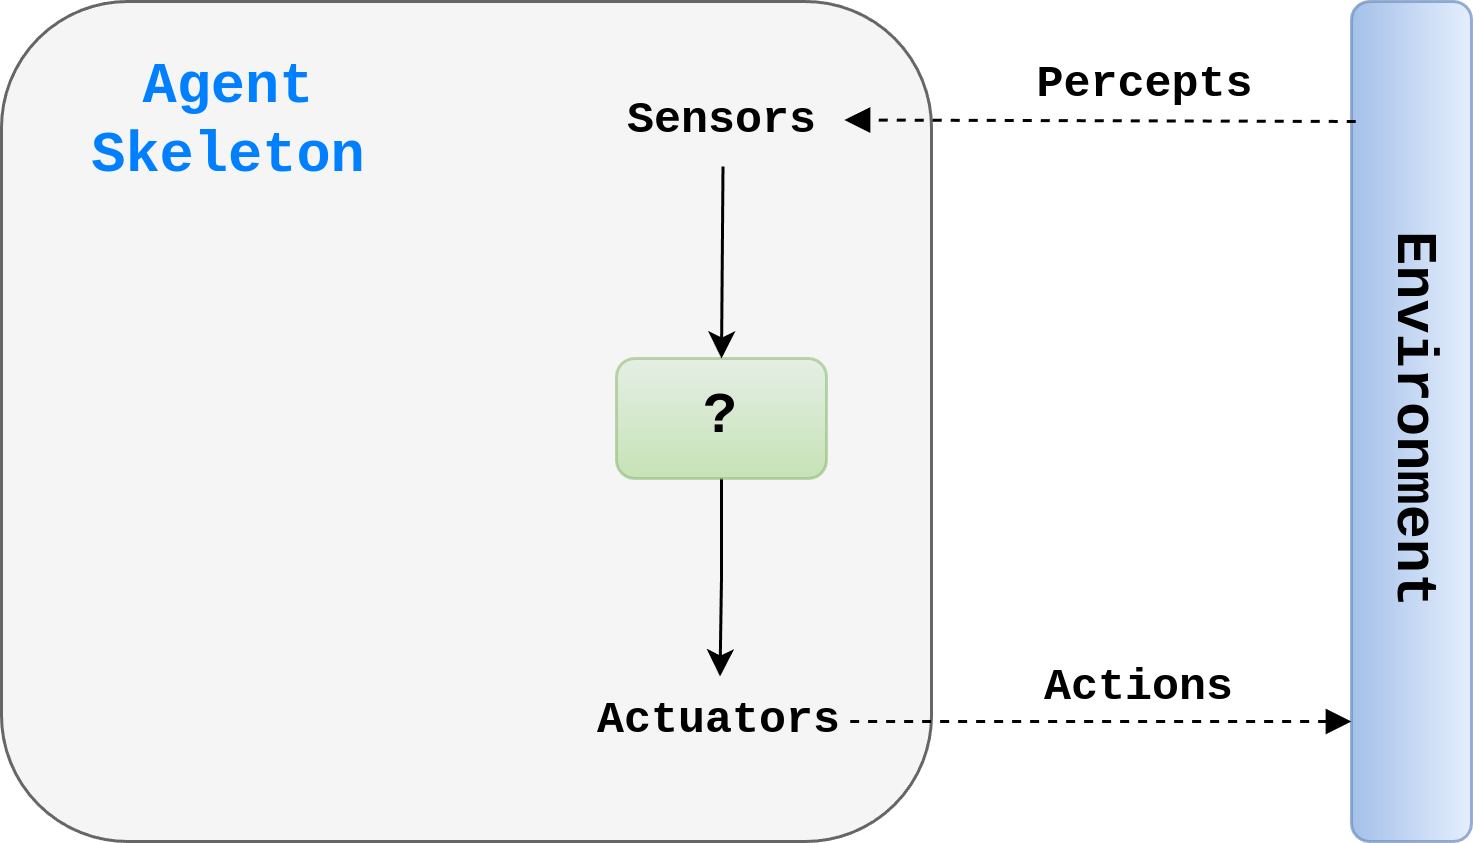
\includegraphics[
        width=0.5\linewidth,
        height=4cm,
        keepaspectratio
    ]{images/artificial-intelligence/ai-agents/agents-skeleton.png}
    \caption*{Agents interact with environments through sensors and actuators. \cite{common/online/tools/draw.io}}
\end{figure}


\begin{enumerate}
    \item \textbf{Agent}: An agent is anything that can be viewed as perceiving its environment through sensors and acting upon that environment through actuators.
    \hfill \cite{ai/book/Artificial-Intelligence-A-Modern-Approach/Russell-Norvig}
    \\
    \verb|agent = architecture + (agent) program|
    \hfill \cite{ai/book/Artificial-Intelligence-A-Modern-Approach/Russell-Norvig}

    \item \textbf{Environment}: environment refers to everything outside the agent that it interacts with.
    \hfill \cite{common/online/chatgpt}
    \\
    The “geography” of the environment is known \textbf{a priori}.
    \hfill \cite{ai/book/Artificial-Intelligence-A-Modern-Approach/Russell-Norvig}
    \\
    "A priori" : Knowledge or assumptions made before data is observed (e.g., predefined rules, constraints).
    \hfill \cite{common/online/chatgpt}

    \item \textbf{Sensors}: A sensor is any mechanism that allows an AI agent to perceive its environment by gathering information. This can be physical (hardware) or virtual (software).
    \hfill \cite{common/online/chatgpt}

    \item \textbf{Actuators}: An actuator is any mechanism that allows an AI agent to affect or change its environment by performing actions.
    \hfill \cite{common/online/chatgpt}

    \item \textbf{Percept}: agent’s perceptual inputs at any given instant
    \hfill \cite{ai/book/Artificial-Intelligence-A-Modern-Approach/Russell-Norvig}

    \item \textbf{Percept Sequence}: it is the complete history of everything the agent has ever perceived. In general, an agent’s choice of action at any given instant can depend on the entire percept sequence observed to date, but \textbf{not} on anything it hasn’t perceived.
    \hfill \cite{ai/book/Artificial-Intelligence-A-Modern-Approach/Russell-Norvig}

    \item \textbf{Agent Function}: maps any given percept sequence to an action; describes agent’s behavior; an external characterization of the agent; The agent function is an abstract mathematical description; takes the entire percept history
    \hfill \cite{ai/book/Artificial-Intelligence-A-Modern-Approach/Russell-Norvig}

    \item \textbf{Agent Program}: internal implementation of the agent function for an artificial agent; the agent program is a concrete implementation, running within some physical system. The agent program takes just the current percept as input because nothing more is available from the environment; if the agent’s actions need to depend on the entire percept sequence, the agent will have to remember the percepts.
    \hfill \cite{ai/book/Artificial-Intelligence-A-Modern-Approach/Russell-Norvig}

    \item \textbf{Architecture}: computing device with physical sensors and actuators on which the agent program is running.
    \hfill \cite{ai/book/Artificial-Intelligence-A-Modern-Approach/Russell-Norvig}

    \item \textbf{Performance Measure}: It evaluates any given sequence of environment states.
    \hfill \cite{ai/book/Artificial-Intelligence-A-Modern-Approach/Russell-Norvig}

    \item \textbf{Rational Agent}: A rational agent is one that does the right thing
    \hfill \cite{ai/book/Artificial-Intelligence-A-Modern-Approach/Russell-Norvig}
    \\
    For each possible percept sequence, a rational agent should select an action that is expected to maximize its performance measure, given the evidence provided by the percept sequence and whatever built-in knowledge the agent has.
    \hfill \cite{ai/book/Artificial-Intelligence-A-Modern-Approach/Russell-Norvig}
    \\
    Rationality is not the same as perfection.
    \hfill \cite{ai/book/Artificial-Intelligence-A-Modern-Approach/Russell-Norvig}
    \\
    Rationality maximizes \textbf{expected} performance, while perfection maximizes \textbf{actual} performance.
    \hfill \cite{ai/book/Artificial-Intelligence-A-Modern-Approach/Russell-Norvig}
    \\
    Our definition of rationality does not require omniscience, then, because the rational choice depends only on the percept sequence to date
    \hfill \cite{ai/book/Artificial-Intelligence-A-Modern-Approach/Russell-Norvig}


    \item \textbf{Omniscient Agent}: An omniscient agent knows the actual outcome of its actions and can act accordingly; but omniscience is impossible in reality.
    \hfill \cite{ai/book/Artificial-Intelligence-A-Modern-Approach/Russell-Norvig}


    \item \textbf{Information Gathering}: It is doing actions in order to modify future percepts.
    \hfill \cite{ai/book/Artificial-Intelligence-A-Modern-Approach/Russell-Norvig}



    \item When an agent is plunked down in an environment, it generates a sequence of actions according to the percepts it receives. This sequence of actions causes the environment to go through a sequence of states. If the sequence is desirable, then the agent has performed well.
    \hfill \cite{ai/book/Artificial-Intelligence-A-Modern-Approach/Russell-Norvig}

    \item  If we define success in terms of agent’s opinion of its own performance, an agent could achieve perfect rationality simply by deluding itself that its performance was perfect.
    \hfill \cite{ai/book/Artificial-Intelligence-A-Modern-Approach/Russell-Norvig}

    \item Human agents in particular are notorious for “sour grapes” - believing they did not really want something (e.g., a Nobel Prize) after not getting it.
    \hfill \cite{ai/book/Artificial-Intelligence-A-Modern-Approach/Russell-Norvig}

    \item As a general rule, it is better to design performance measures according to what one actually wants in the environment, rather than according to how one thinks the agent should behave.
    \hfill \cite{ai/book/Artificial-Intelligence-A-Modern-Approach/Russell-Norvig}

    \item The agent’s initial configuration could reflect some prior knowledge of the environment, but as the agent gains experience this may be modified and augmented. There are extreme cases in which the environment is completely known \textbf{a priori}. In such cases, the agent need not perceive or learn; it simply acts correctly. Such agents are fragile.
    \hfill \cite{ai/book/Artificial-Intelligence-A-Modern-Approach/Russell-Norvig}

    \item To the extent that an agent relies on the prior knowledge of its designer rather than on its own percepts, we say that the agent \textbf{lacks autonomy}.
    \hfill \cite{ai/book/Artificial-Intelligence-A-Modern-Approach/Russell-Norvig}
    \\
    A rational agent should be \textbf{autonomous} - it should learn what it can to compensate for partial or incorrect prior knowledge.
    \hfill \cite{ai/book/Artificial-Intelligence-A-Modern-Approach/Russell-Norvig}

    \item After sufficient experience of its environment, the behavior of a rational agent can become effectively \textbf{independent} of its prior knowledge. Hence, the incorporation of learning allows one to design a single rational agent that will succeed in a vast variety of environments.
    \hfill \cite{ai/book/Artificial-Intelligence-A-Modern-Approach/Russell-Norvig}


\end{enumerate}




\section{Task Environment/ Problem \cite{ai/book/Artificial-Intelligence-A-Modern-Approach/Russell-Norvig}}\label{AI: Agents/Task Environment or Problem}


\begin{enumerate}
    \item Task environments are essentially the “problems” to which rational agents are the “solutions.”
    \hfill \cite{ai/book/Artificial-Intelligence-A-Modern-Approach/Russell-Norvig}


\end{enumerate}

\subsection{PEAS: Defining Problem}

\begin{enumerate}
    \item \textbf{Performance}:
    \begin{enumerate}
        \item Desirable qualities
        \hfill \cite{ai/book/Artificial-Intelligence-A-Modern-Approach/Russell-Norvig}

        \item Defines how the success of the agent is evaluated.
        \hfill \cite{common/online/chatgpt}

        \item[] \textbf{Example}: In a self-driving car, performance can be measured by safety, fuel efficiency, and reaching the destination on time.
        \hfill \cite{common/online/chatgpt}
    \end{enumerate}

    \item \textbf{Environment}:
    \begin{enumerate}
        \item The surroundings in which the agent operates.
        \hfill \cite{common/online/chatgpt}

        \item[] \textbf{Example}: For a self-driving car, the environment includes roads, traffic, pedestrians, and weather conditions.
        \hfill \cite{common/online/chatgpt}
    \end{enumerate}

    \item \textbf{Actuators}:
    \begin{enumerate}
        \item The mechanisms that allow the agent to take action.
        \hfill \cite{common/online/chatgpt}

        \hfill Can be hardware or software.

        \item[] \textbf{Example}: A self-driving car uses its steering wheel, accelerator, and brakes as actuators.
        \hfill \cite{common/online/chatgpt}
    \end{enumerate}

    \item \textbf{Sensors}:
    \begin{enumerate}
        \item The components that allow the agent to perceive its environment.
        \hfill \cite{common/online/chatgpt}

        \hfill Can be hardware or software.

        \item[] \textbf{Example}: A self-driving car has cameras, LiDAR, GPS, and speed sensors.
        \hfill \cite{common/online/chatgpt}
    \end{enumerate}

\end{enumerate}


\vspace{0.3cm}

\textbf{Note}:
\begin{enumerate}
    \item some \textbf{software agents} (or \textbf{software robots} or \textbf{softbots}) exist in rich, unlimited domains.
    \hfill \cite{ai/book/Artificial-Intelligence-A-Modern-Approach/Russell-Norvig}


\end{enumerate}


\clearpage
\subsection{Properties of Task Environments \cite{ai/book/Artificial-Intelligence-A-Modern-Approach/Russell-Norvig}}

\subsubsection{Fully observable, partially observable, unobservable}
\begin{enumerate}
    \item \textbf{fully observable}: If an agent’s sensors give it access to the complete state of the environment at each point in time, then we say that the task environment is fully observable.
    A task environment is effectively fully observable if the sensors detect all aspects that are \textbf{relevant} to the choice of action; relevance, in turn, depends on the performance measure.
    Fully observable environments are convenient because the agent need not maintain any internal state to keep track of the world.
    \hfill \cite{ai/book/Artificial-Intelligence-A-Modern-Approach/Russell-Norvig}

    \vspace{0.2cm}

    \item \textbf{partially observable}: An environment might be partially observable because of noisy and inaccurate sensors or because parts of the state are simply missing from the sensor data.
    \hfill \cite{ai/book/Artificial-Intelligence-A-Modern-Approach/Russell-Norvig}

    \vspace{0.2cm}

    \item \textbf{unobservable}: If the agent has no sensors at all then the environment is unobservable.
    The agent’s goals may still be achievable, sometimes with certainty.
    \hfill \cite{ai/book/Artificial-Intelligence-A-Modern-Approach/Russell-Norvig}
\end{enumerate}

\subsubsection{Single agent, multi-agent}
\begin{enumerate}
    \item \textbf{Single agent}:  Only 1 agent is interacting in the given environment.

    \item \textbf{Multi-agent}: More than 1 agent (of same type or different types) interact in the given environment.
    \begin{enumerate}
        \item \textbf{Competitive Multi-agent}: Agents maximize their own performance at cost of other agents' performance.
        \\
        Examples: 2 agents playing Chess against each other; taxi-driving (competing for parking space)

        \item \textbf{Cooperative Multi-agent}: Agents take actions to maximize collective performance.
        \\
        Example: taxi-driving (avoiding collisions)

        \vspace{0.3cm}

        \item \textbf{communication} often emerges as a rational behavior in multiagent environments; in some competitive environments, \textbf{randomized behavior} is rational because it avoids the pitfalls of predictability.
        \hfill \cite{ai/book/Artificial-Intelligence-A-Modern-Approach/Russell-Norvig}
    \end{enumerate}

\end{enumerate}


\subsubsection{Deterministic, stochastic, uncertain, nondeterministic}
\begin{enumerate}
    \item If the next state of the environment is completely determined by the current state and the action executed by the agent, then we say the environment is \textbf{deterministic}; otherwise, it is \textbf{stochastic}.
    \hfill \cite{ai/book/Artificial-Intelligence-A-Modern-Approach/Russell-Norvig}

    \item In principle, an agent need not worry about uncertainty in a fully observable, deterministic environment.
    \hfill \cite{ai/book/Artificial-Intelligence-A-Modern-Approach/Russell-Norvig}

    \item  If the environment is partially observable, however, then it could appear to be stochastic. Most real situations are so complex that it is impossible to keep track of all the unobserved aspects; for practical purposes, they must be treated as \textbf{stochastic}.
    \hfill \cite{ai/book/Artificial-Intelligence-A-Modern-Approach/Russell-Norvig}
    \\
    It implies that uncertainty about outcomes is quantified in terms of \textit{probabilities}.
    \hfill \cite{ai/book/Artificial-Intelligence-A-Modern-Approach/Russell-Norvig}

    \item  We say an environment is \textbf{uncertain} if it is not fully observable or not deterministic.
    \hfill \cite{ai/book/Artificial-Intelligence-A-Modern-Approach/Russell-Norvig}

    \item A \textbf{nondeterministic} environment is one in which actions are characterized by their possible outcomes, but no probabilities are attached to them. Non-deterministic environment descriptions are usually associated with performance measures that require the agent to succeed for all possible outcomes of its actions.
    \hfill \cite{ai/book/Artificial-Intelligence-A-Modern-Approach/Russell-Norvig}
\end{enumerate}


\subsubsection{Episodic, sequential}
\begin{enumerate}
    \item In an \textbf{episodic} task environment, the agent’s experience is divided into atomic episodes. In each episode the agent receives a percept and then performs a single action. Crucially, the next episode does not depend on the actions taken in previous episodes. Episodic environments are much simpler than sequential environments because the agent does not need to think ahead.
    \hfill \cite{ai/book/Artificial-Intelligence-A-Modern-Approach/Russell-Norvig}

    \item In \textbf{sequential} environments, on the other hand, the current decision could affect all future decisions.
    \hfill \cite{ai/book/Artificial-Intelligence-A-Modern-Approach/Russell-Norvig}
\end{enumerate}


\subsubsection{Static, dynamic, semidynamic}
\begin{enumerate}
    \item If the environment can change while an agent is deliberating, then we say the environment is \textbf{dynamic} for that agent; otherwise, it is \textbf{static}.
    \hfill \cite{ai/book/Artificial-Intelligence-A-Modern-Approach/Russell-Norvig}

    \item Static environments are easy to deal with because the agent need not keep looking at the world while it is deciding on an action, nor need it worry about the passage of time.
    \hfill \cite{ai/book/Artificial-Intelligence-A-Modern-Approach/Russell-Norvig}

    \item  Dynamic environments, on the other hand, are continuously asking the agent what it wants to do; if it hasn’t decided yet, that counts as deciding to do nothing.
    \hfill \cite{ai/book/Artificial-Intelligence-A-Modern-Approach/Russell-Norvig}

    \item If the environment itself does not change with the passage of time but the agent’s performance score does, then we say the environment is \textbf{semidynamic}.
    \hfill \cite{ai/book/Artificial-Intelligence-A-Modern-Approach/Russell-Norvig}
\end{enumerate}


\subsubsection{Discrete, continuous}
\begin{enumerate}
    \item The discrete/continuous distinction applies to the state of the environment, to the way \textit{time} is handled, and to the percepts and actions of the agent.
    \hfill \cite{ai/book/Artificial-Intelligence-A-Modern-Approach/Russell-Norvig}


\end{enumerate}



\subsubsection{Known, unknown}
\begin{enumerate}
    \item Strictly speaking, this distinction refers not to the environment itself but to the agent’s (or designer’s) state of knowledge about the “laws of physics” of the environment.
    \hfill \cite{ai/book/Artificial-Intelligence-A-Modern-Approach/Russell-Norvig}

    \item In a \textbf{known} environment, the outcomes (or outcome probabilities if the environment is stochastic) for all actions are given.
    \hfill \cite{ai/book/Artificial-Intelligence-A-Modern-Approach/Russell-Norvig}

    \item  if the environment is \textbf{unknown}, the agent will have to learn how it works in order to make good decisions.
    \hfill \cite{ai/book/Artificial-Intelligence-A-Modern-Approach/Russell-Norvig}


\end{enumerate}



\subsubsection*{Examples \cite{ai/book/Artificial-Intelligence-A-Modern-Approach/Russell-Norvig}}

\begin{customArrayStretch}{1.3}
\begin{tabular}{ | >{\fontsize{10}{10}\arraybackslash}l | l l l l l l | }
    \hline

    \textbf{Task Environment} & \textbf{Observable} & \textbf{Agents} &
        \textbf{Deterministic} & \textbf{Episodic} &
        \textbf{Static} & \textbf{Discrete} \\

    \hline\hline

    \textbf{Crossword puzzle} & Fully & Single & Deterministic & Sequential & Static & Discrete \\

    \textbf{Chess with a clock} & Fully & Multi & Deterministic & Sequential & Semi & Discrete \\

    \hline

    \textbf{Poker} & Partially & Multi & Stochastic & Sequential & Static & Discrete \\

    \textbf{Backgammon} & Fully & Multi & Stochastic & Sequential & Static & Discrete \\

    \hline

    \textbf{Taxi driving} & Partially & Multi & Stochastic & Sequential & Dynamic & Continuous \\

    \textbf{Medical diagnosis} & Partially & Single & Stochastic & Sequential & Dynamic & Continuous \\

    \hline

    \textbf{Image analysis} & Fully & Single & Deterministic & Episodic & Semi & Continuous \\

    \textbf{Part-picking robot} & Partially & Single & Stochastic & Episodic & Dynamic & Continuous \\

    \hline

    \textbf{Refinery controller} & Partially & Single & Stochastic & Sequential & Dynamic & Continuous \\

    \textbf{Interactive English tutor} & Partially & Multi & Stochastic & Sequential & Dynamic & Discrete \\

    \hline
\end{tabular}
\end{customArrayStretch}



\subsubsection*{Note}
\begin{enumerate}
    \item  the distinction between known and unknown environments is not the same as the one between fully and partially observable environments.
    \hfill \cite{ai/book/Artificial-Intelligence-A-Modern-Approach/Russell-Norvig}

    \item It is quite possible for a \textbf{known} environment to be \textbf{partially observable}—for example, in solitaire card games, I know the rules but am still unable to see the cards that have not yet been turned over.
    \hfill \cite{ai/book/Artificial-Intelligence-A-Modern-Approach/Russell-Norvig}

    \item an \textbf{unknown} environment can be \textbf{fully observable}—in a new video game, the screen may show the entire game state but I still don’t know what the buttons do until I try them.
    \hfill \cite{ai/book/Artificial-Intelligence-A-Modern-Approach/Russell-Norvig}

    \item \textbf{environment class}: A category or set of related environments from which specific environments are drawn for testing or training agents.
    \hfill \cite{ai/book/Artificial-Intelligence-A-Modern-Approach/Russell-Norvig, common/online/chatgpt}

    \item \textbf{environment generator}: An environment generator is a tool or function that creates individual environments sampled from an environment class. It automates the creation of diverse scenarios for training or evaluating agents.
    \hfill \cite{ai/book/Artificial-Intelligence-A-Modern-Approach/Russell-Norvig, common/online/chatgpt}


\end{enumerate}



\section{Agent State Representations}\label{AI: Agents/Agent State Representations}

\begin{figure}[H]
    \centering
    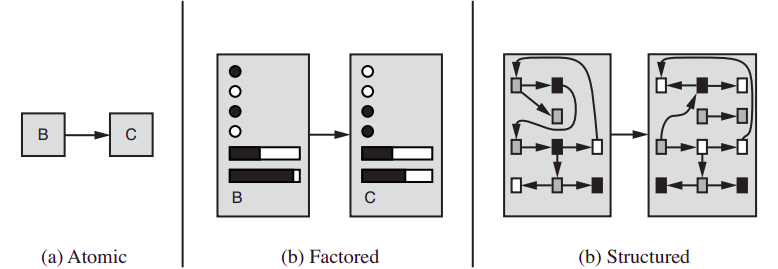
\includegraphics[
        width=\linewidth,
        height=6cm,
        keepaspectratio,
    ]{images/artificial-intelligence/ai-agents/state-representations.png}
    \caption*{
    Three ways to represent states and the transitions between them.
    \\
    \textbf{(a)} Atomic representation: a state (such as B or C) is a black box with no internal structure;  
    \hfill \cite{ai/book/Artificial-Intelligence-A-Modern-Approach/Russell-Norvig}
    \\
    \textbf{(b)} Factored representation: a state consists of a vector of attribute values; values can be Boolean, realvalued, or one of a fixed set of symbols.
    \hfill \cite{ai/book/Artificial-Intelligence-A-Modern-Approach/Russell-Norvig}
    \\
    \textbf{(c)} Structured representation: a state includes objects, each of which may have attributes of its own as well as relationships to other objects.
    \hfill \cite{ai/book/Artificial-Intelligence-A-Modern-Approach/Russell-Norvig}
}
\end{figure}



\begin{enumerate}[itemsep=0.2cm]
    \item Roughly speaking, a more expressive representation can capture, at least as concisely, everything a less expressive one can capture, plus some more. 
    \hfill \cite{ai/book/Artificial-Intelligence-A-Modern-Approach/Russell-Norvig}

    \item Often, the more expressive language is much more concise; for example, the rules of chess can be written in a page or two of a structured-representation language such as first-order logic but require thousands of pages when written in a factored-representation language such as propositional logic.
    \hfill \cite{ai/book/Artificial-Intelligence-A-Modern-Approach/Russell-Norvig}

    \item reasoning and learning become more complex as the expressive power of the representation increases.
    \hfill \cite{ai/book/Artificial-Intelligence-A-Modern-Approach/Russell-Norvig}

    \item To gain the benefits of expressive representations while avoiding their drawbacks, intelligent systems for the real world may need to operate at all points along the axis simultaneously.
    \hfill \cite{ai/book/Artificial-Intelligence-A-Modern-Approach/Russell-Norvig}
\end{enumerate}






\subsection{Atomic representation}

\begin{enumerate}[itemsep=0.2cm]
    \item each state of the world is indivisible - it has no internal structure. 
    \hfill \cite{ai/book/Artificial-Intelligence-A-Modern-Approach/Russell-Norvig}

    \item two different atomic states have nothing in common—they are just different black boxes
    \hfill \cite{ai/book/Artificial-Intelligence-A-Modern-Approach/Russell-Norvig}

    \item Algorithms/ areas that work with atomic representations - or, at least, they treat representations as if they were atomic:
    \begin{enumerate}
        \item Search and game-playing
        \hfill \cite{ai/book/Artificial-Intelligence-A-Modern-Approach/Russell-Norvig}

        \item Hidden Markov models
        \hfill \cite{ai/book/Artificial-Intelligence-A-Modern-Approach/Russell-Norvig}

        \item Markov decision processes
        \hfill \cite{ai/book/Artificial-Intelligence-A-Modern-Approach/Russell-Norvig}
    \end{enumerate}
\end{enumerate}



\subsection{Factored representation}

\begin{enumerate}[itemsep=0.2cm]
    \item A factored representation splits up each state into a fixed set of \textbf{variables} or \textbf{attributes}, each of which can have a \textbf{value}.
    \hfill \cite{ai/book/Artificial-Intelligence-A-Modern-Approach/Russell-Norvig}

    \item two different factored states can \textbf{share} some attributes (such as being at some particular GPS location) and not others (such as having lots of gas or having no gas)
    \\
    this makes it much easier to work out how to turn one state into another
    \hfill \cite{ai/book/Artificial-Intelligence-A-Modern-Approach/Russell-Norvig}

    \item With factored representations, we can also represent uncertainty - for example, ignorance about the amount of gas in the tank can be represented by leaving that attribute blank.
    \hfill \cite{ai/book/Artificial-Intelligence-A-Modern-Approach/Russell-Norvig}

    \item Algorithms/ areas based on factored representations:
    \begin{enumerate}
        \item constraint satisfaction algorithms
        \hfill \cite{ai/book/Artificial-Intelligence-A-Modern-Approach/Russell-Norvig}

        \item propositional logic
        \hfill \cite{ai/book/Artificial-Intelligence-A-Modern-Approach/Russell-Norvig}

        \item planning
        \hfill \cite{ai/book/Artificial-Intelligence-A-Modern-Approach/Russell-Norvig}

        \item Bayesian networks
        \hfill \cite{ai/book/Artificial-Intelligence-A-Modern-Approach/Russell-Norvig}

    \end{enumerate}
\end{enumerate}








\subsection{Structured representation}


\begin{enumerate}[itemsep=0.2cm]
    \item the world as having things in it that are related to each other, not just variables with values.
    \hfill \cite{ai/book/Artificial-Intelligence-A-Modern-Approach/Russell-Norvig}

    \item almost everything that humans express in natural language concerns objects and their relationships
    \hfill \cite{ai/book/Artificial-Intelligence-A-Modern-Approach/Russell-Norvig}

    \item Algorithms/ areas based on factored representations:
    \begin{enumerate}
        \item relational databases
        \hfill \cite{ai/book/Artificial-Intelligence-A-Modern-Approach/Russell-Norvig}

        \item first-order logic
        \hfill \cite{ai/book/Artificial-Intelligence-A-Modern-Approach/Russell-Norvig}

        \item first-order probability models 
        \hfill \cite{ai/book/Artificial-Intelligence-A-Modern-Approach/Russell-Norvig}

        \item knowledge-based learning
        \hfill \cite{ai/book/Artificial-Intelligence-A-Modern-Approach/Russell-Norvig}

        \item natural language understanding
        \hfill \cite{ai/book/Artificial-Intelligence-A-Modern-Approach/Russell-Norvig}
    \end{enumerate}
\end{enumerate}






\chapter{AI: Agent Programs}


\section{Table Driven Agent}\label{AI: Agent Programs/Table Driven Agent}


\begin{figure}[H]
    \centering
    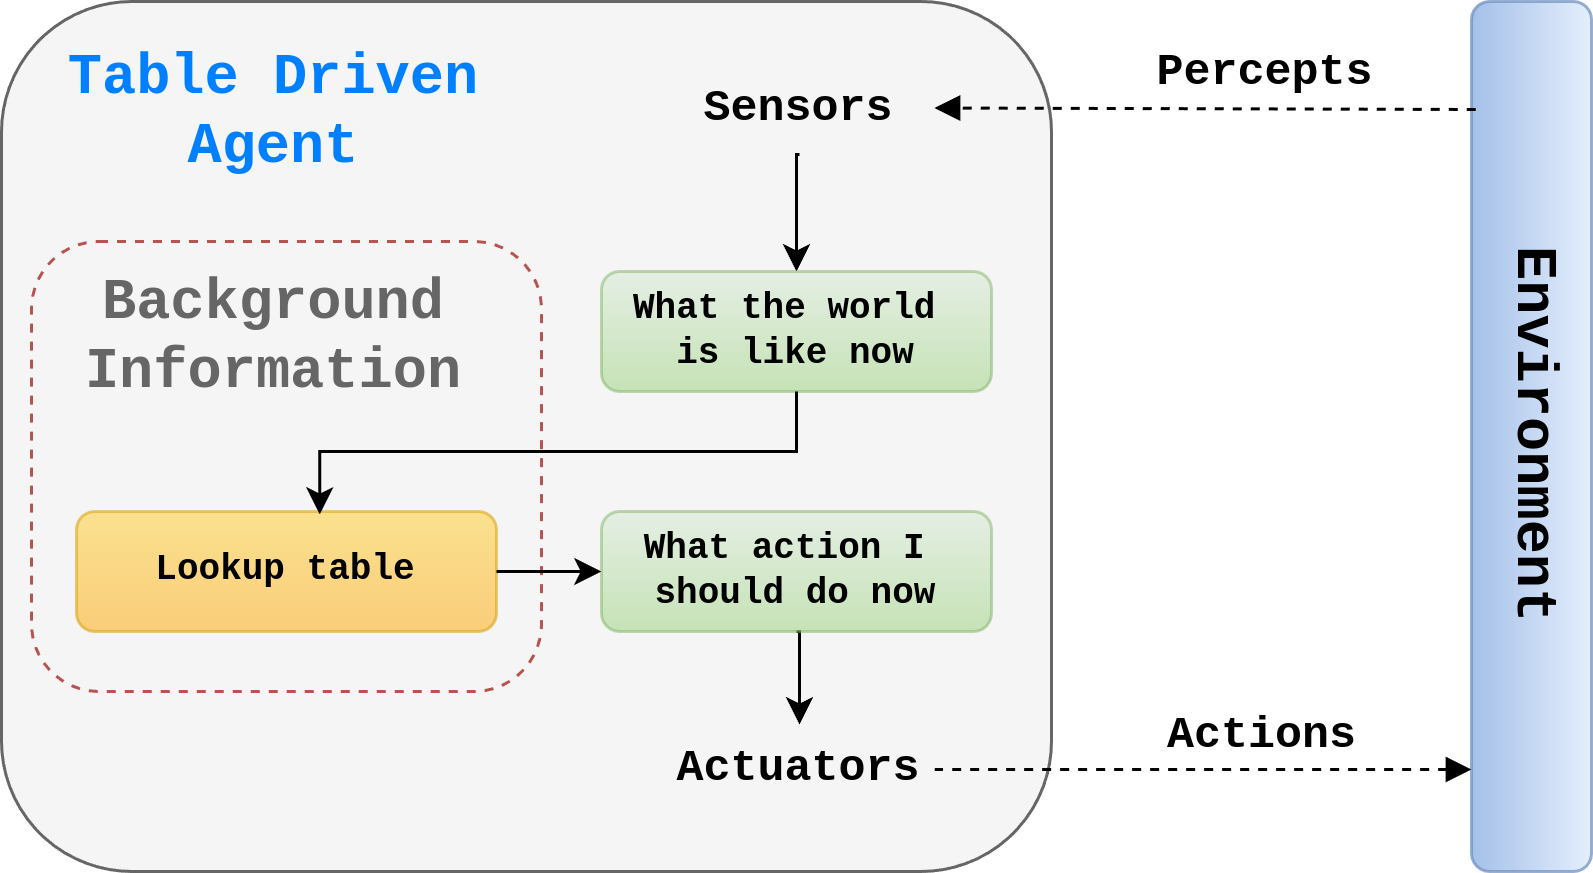
\includegraphics[
        width=0.5\linewidth,
        height=4cm,
        keepaspectratio
    ]{images/artificial-intelligence/ai-agents/agents-table-driven-agent.png}
    \caption*{Schematic diagram of a table driven agent. \cite{common/online/tools/draw.io}}
\end{figure}

\begin{longtable}{l l}

$\mathcal{P}$ & set of possible percepts \\

$T$ & lifetime of agent (total number of percepts) \\

\end{longtable}


\vspace{0.5cm}

\begin{enumerate}
    \item Number of entries in table: $
        \dsum_{t=1}^T \dabs{\mathcal{P}}^t
    $
    \hfill \cite{ai/book/Artificial-Intelligence-A-Modern-Approach/Russell-Norvig}

    \item Sometimes the number of entries can be ridiculously large number due to the combinations of percepts and length of percept sequence.\\
    \textbf{Example}: Consider the \textit{automated taxi}: the visual input from a single camera comes in at the rate of roughly $27$ megabytes per second ($30$ frames per second, $640 \times 480$ pixels with $24$ bits of color information). This gives a lookup table with over $10^{250,000,000,000}$ entries for an hour’s driving.
    \hfill \cite{ai/book/Artificial-Intelligence-A-Modern-Approach/Russell-Norvig}
    \\
    It means:
    \begin{enumerate}
        \item no physical agent in this universe will have the space to store the table
        \hfill \cite{ai/book/Artificial-Intelligence-A-Modern-Approach/Russell-Norvig}

        \item the designer would not have time to create the table
        \hfill \cite{ai/book/Artificial-Intelligence-A-Modern-Approach/Russell-Norvig}

        \item no agent could ever learn all the right table entries from its experience
        \hfill \cite{ai/book/Artificial-Intelligence-A-Modern-Approach/Russell-Norvig}

        \item even if the environment is simple enough to yield a feasible table size, the designer still has no guidance about how to fill in the table entries
        \hfill \cite{ai/book/Artificial-Intelligence-A-Modern-Approach/Russell-Norvig}

    \end{enumerate}
\end{enumerate}

\vspace{0.5cm}

\begin{algorithm}[H]
    \caption{The \textsc{Table-Driven-Agent} program is invoked for each new percept and returns an action each time. It retains the complete percept sequence in memory. \cite{ai/book/Artificial-Intelligence-A-Modern-Approach/Russell-Norvig}}

    \SetKwFunction{FUNCTION}{\textsc{Table-Driven-Agent}}
    \SetKwProg{Fn}{function}{ returns \normalfont an action}{end}
    \Fn{\FUNCTION{ percept }}{
        \textbf{persistent}:\\

        \hspace{0.4cm} $percepts$, a sequence, initially empty\\

        \hspace{0.4cm} $table$, a table of actions, indexed by percept sequences, initially fully specified \\

        \ \\

        append $percept$ to the end of $percepts$ \\

        $action$ $\gets$ \textsc{Lookup}($\ percepts,\ table\ $) \\

        \Return $action$
    }
\end{algorithm}





\section{Simple Reflex Agent}\label{AI: Agent Programs/Simple Reflex Agent}


\begin{figure}[H]
    \centering
    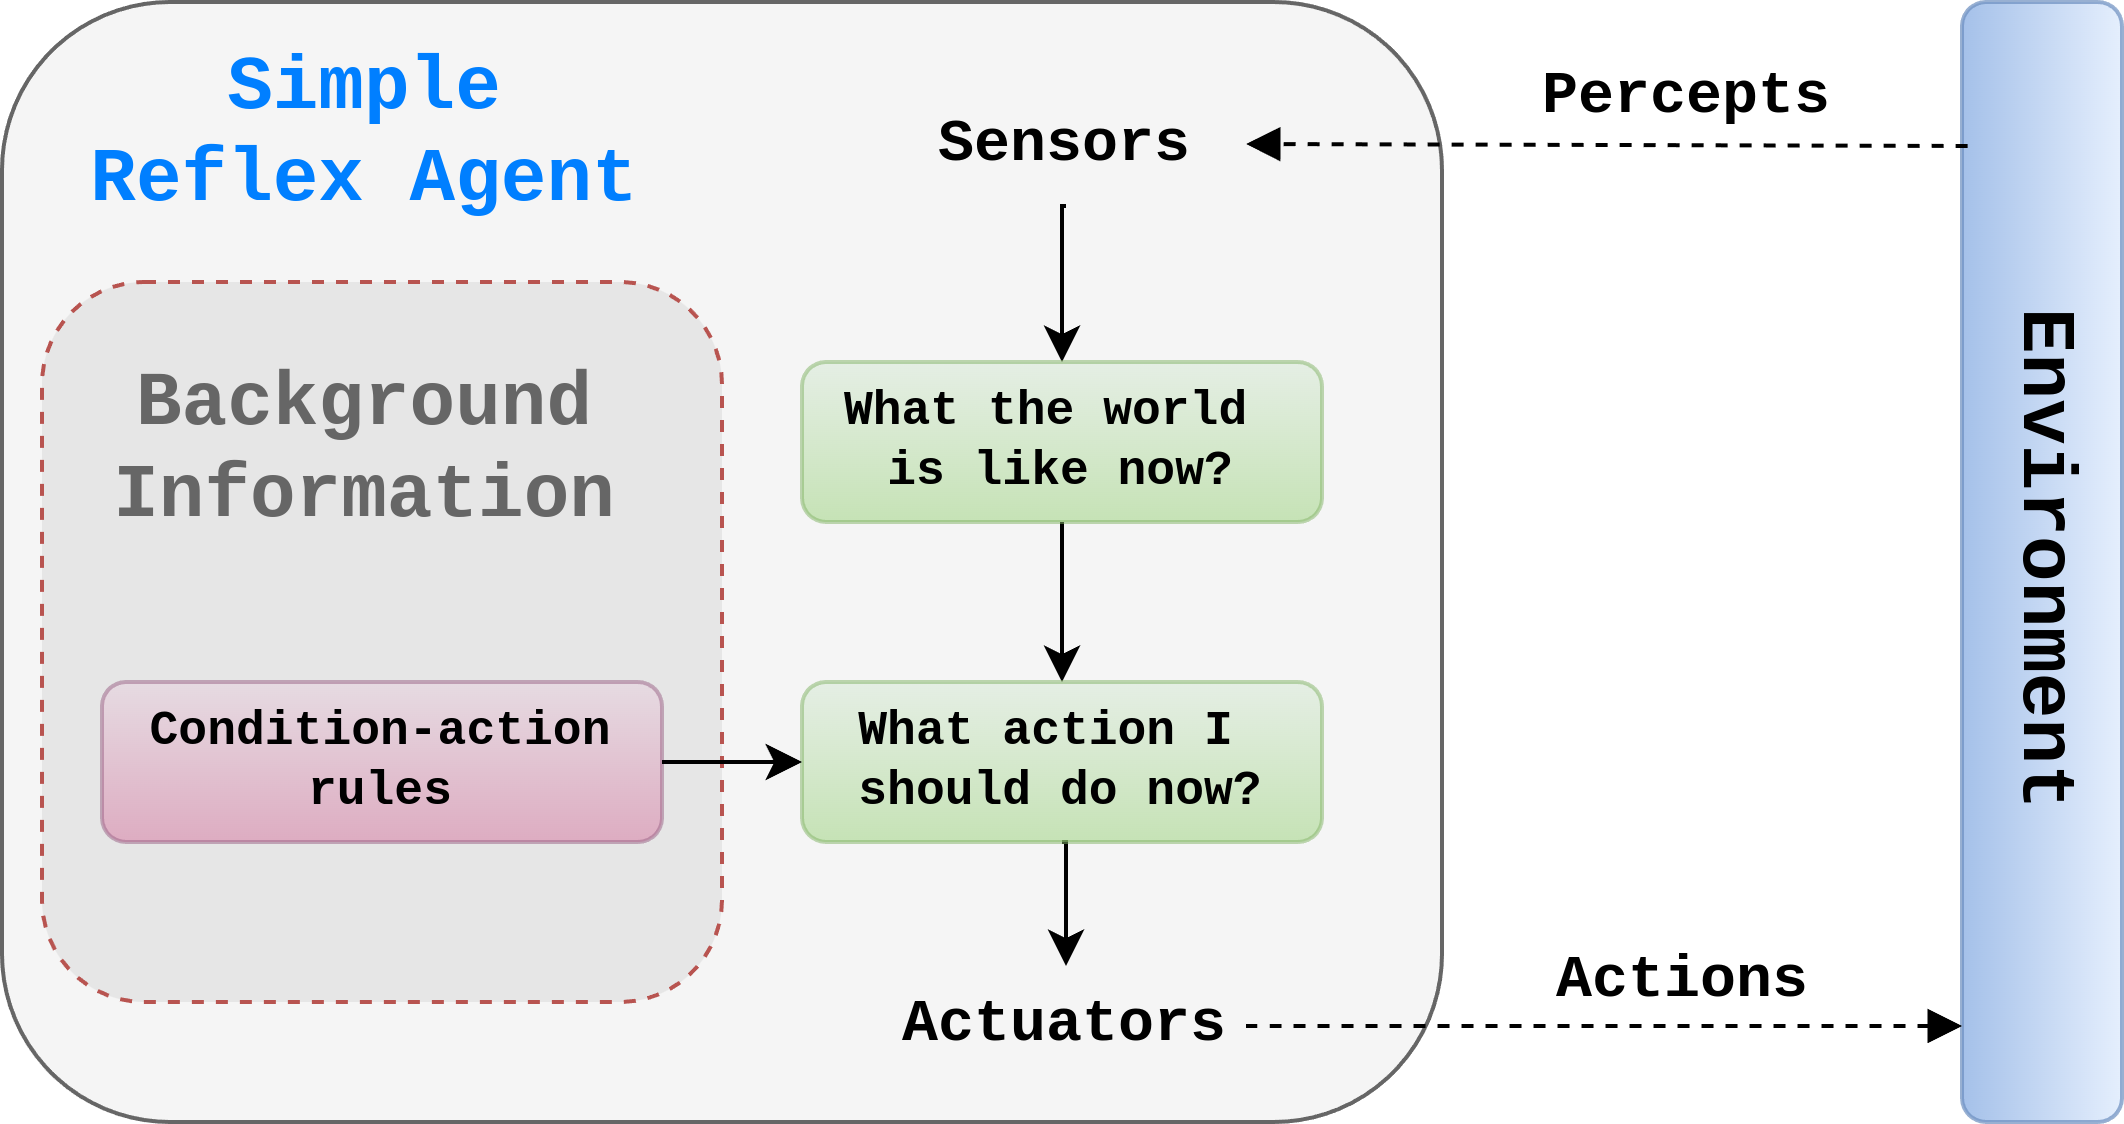
\includegraphics[
        width=0.5\linewidth, 
        height=4cm, 
        keepaspectratio
    ]{images/artificial-intelligence/ai-agents/agents-Simple-reflex-agent.png}
    \caption*{Schematic diagram of a simple reflex agent. \cite{common/online/tools/draw.io}}
\end{figure}

\begin{enumerate}
    \item simplest kind of agent
    \hfill \cite{ai/book/Artificial-Intelligence-A-Modern-Approach/Russell-Norvig}

    \item These agents select actions on the basis of the \textit{current} percept, ignoring the rest of the percept history.
    \hfill \cite{ai/book/Artificial-Intelligence-A-Modern-Approach/Russell-Norvig}

    \item \textbf{condition-action rule/ situation-action rules/ productions/ if-then rules}:\\
    A condition-action rule is a basic decision-making structure used in reflex agents and rule-based systems.
    \hfill \cite{ai/book/Artificial-Intelligence-A-Modern-Approach/Russell-Norvig, common/online/chatgpt}

    \item the description in terms of “rules” and “matching” is purely conceptual; actual implementations can be as simple as a collection of logic gates implementing a Boolean circuit.
    \hfill \cite{ai/book/Artificial-Intelligence-A-Modern-Approach/Russell-Norvig}

    \item Escape from infinite loops is possible if the agent can \textbf{randomize} its actions.  
    A randomized simple reflex agent \textit{might outperform} a deterministic simple reflex agent.
    Randomized behavior of the right kind can be rational in some multi-agent environments. 
    In single-agent environments, randomization is usually \textbf{not} rational. 
    \hfill \cite{ai/book/Artificial-Intelligence-A-Modern-Approach/Russell-Norvig}
    

    \item \textbf{Disadvantage}: limited intelligence
    \hfill \cite{ai/book/Artificial-Intelligence-A-Modern-Approach/Russell-Norvig}

    \item \textbf{Disadvantage}: will work only if the correct decision can be made on the basis of only the current percept—that is, only if the environment is fully observable. Even a little bit of un-observability can cause serious trouble.
    \hfill \cite{ai/book/Artificial-Intelligence-A-Modern-Approach/Russell-Norvig}

    \item \textbf{Disadvantage}: we would have to rewrite many condition–action rules for supporting more situations/ scenarios. 

\end{enumerate}


\vspace{0.5cm}


\begin{algorithm}[H]
    \caption{\textsc{Simple-Reflex-Agent}: It acts according to a rule whose condition matches the current state, as defined by the percept. \cite{ai/book/Artificial-Intelligence-A-Modern-Approach/Russell-Norvig}}

    \SetKwFunction{FUNCTION}{\textsc{Simple-Reflex-Agent}}
    \SetKwProg{Fn}{function}{ returns \normalfont an action}{end}
    \Fn{\FUNCTION{ percept }}{
        \textbf{persistent}: $rules$, a set of condition-action rules \\
        \ \\
        $state$ $\gets$ \textsc{Interpret-Input}( $percept$ )\\
        $rule$ $\gets$ \textsc{Rule-Match}( $state,\ rules$ ) \\
        $action$ $\gets$ $rule$.\textsc{Action} \\
        \Return $action$
    }
\end{algorithm}

\vspace{0.3cm}

\begin{customArrayStretch}{1.2}
\begin{longtable}{l p{12cm} l}

\textsc{Interpret-Input} & 
    generates an abstracted description of the current state from the percept &
    \cite{ai/book/Artificial-Intelligence-A-Modern-Approach/Russell-Norvig} \\

\textsc{Rule-Match} & 
    returns the first rule in the set of rules that matches the given state description &
    \cite{ai/book/Artificial-Intelligence-A-Modern-Approach/Russell-Norvig} \\

\end{longtable}
\end{customArrayStretch}










\section{Model-based reflex agents}\label{AI: Agent Programs/Model-based reflex agents}


\begin{figure}[H]
    \centering
    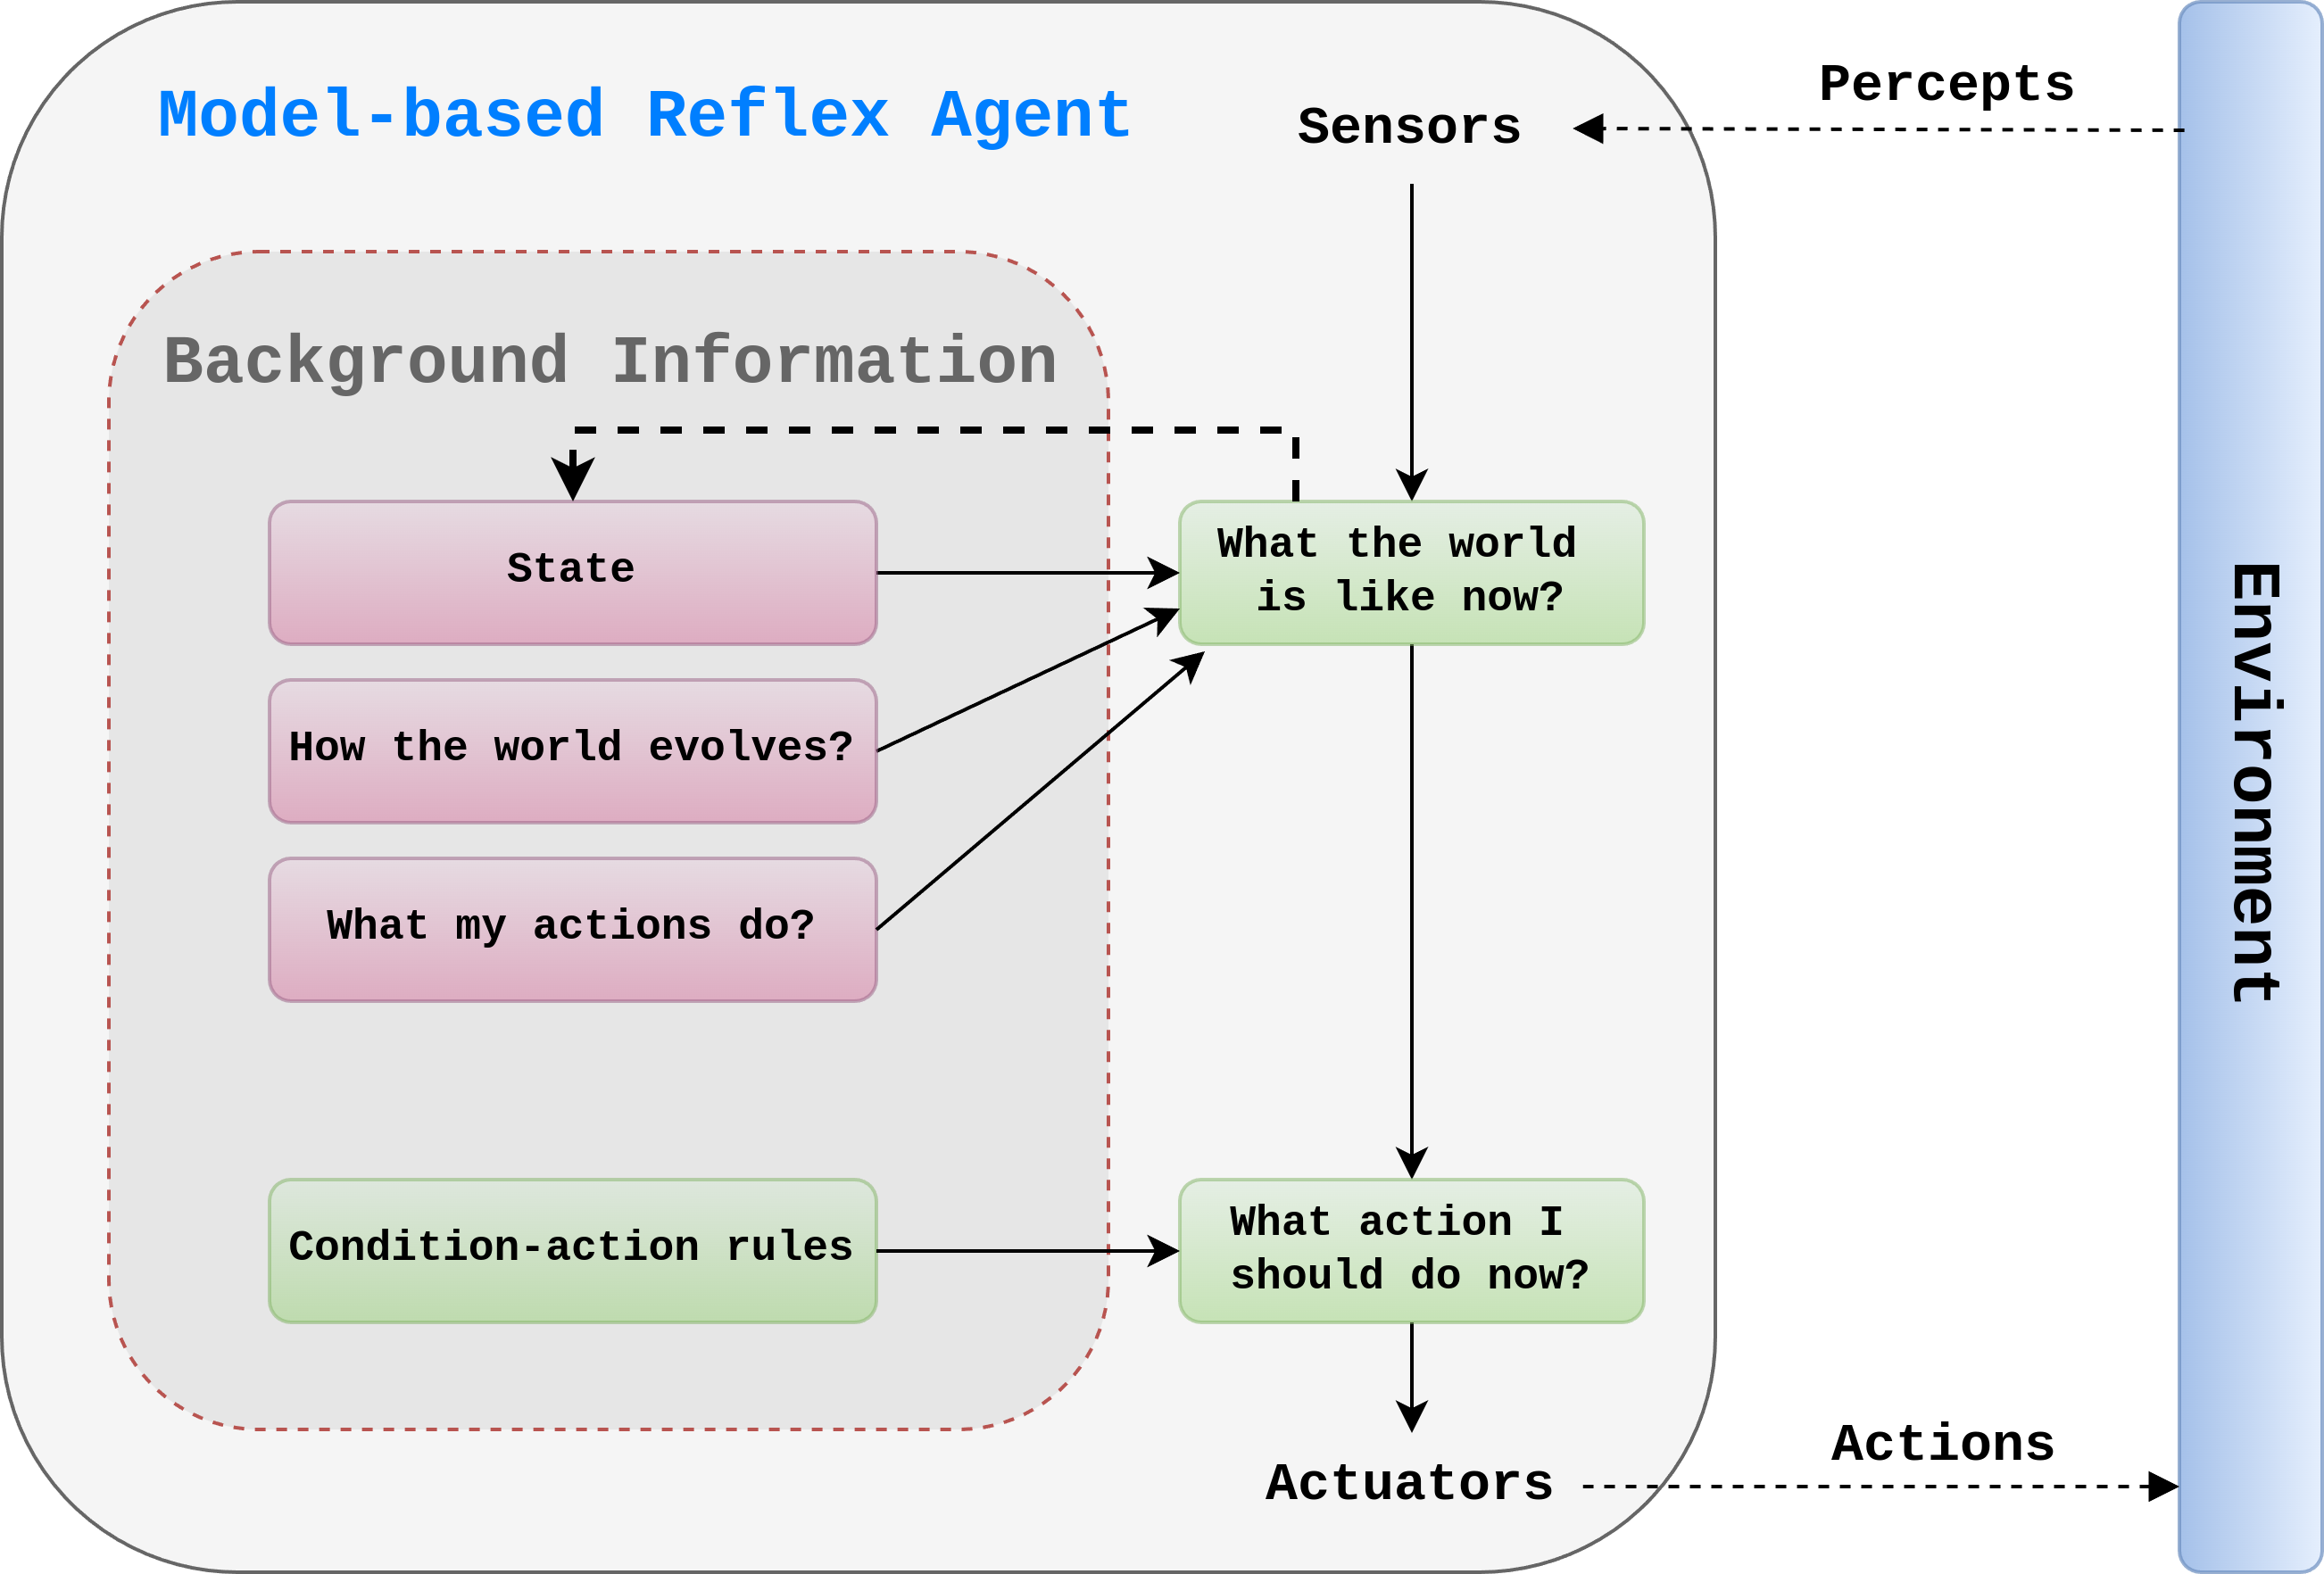
\includegraphics[
        width=0.5\linewidth, 
        height=6cm, 
        keepaspectratio
    ]{images/artificial-intelligence/ai-agents/agents-Model-based-reflex-agent.png}
    \caption*{A model-based reflex agent. \cite{common/online/tools/draw.io}}
\end{figure}


\vspace{0.2cm}

\begin{enumerate}
    \item The most effective way to handle partial observability is for the agent to keep track of the part of the world it can’t see now.
    \hfill \cite{ai/book/Artificial-Intelligence-A-Modern-Approach/Russell-Norvig}

    \item the agent should maintain some sort of internal state that depends on the percept history and thereby reflects at least some of the unobserved aspects of the current state. 
    \hfill \cite{ai/book/Artificial-Intelligence-A-Modern-Approach/Russell-Norvig}

    \item Updating this internal state information as time goes by requires two kinds of knowledge to be encoded in the agent program.
    \begin{enumerate}
        \item we need some information about how the world evolves independently of the agent
        \hfill \cite{ai/book/Artificial-Intelligence-A-Modern-Approach/Russell-Norvig}

        \item we need some information about how the agent’s own actions affect the world
        \hfill \cite{ai/book/Artificial-Intelligence-A-Modern-Approach/Russell-Norvig}
    \end{enumerate}

    \item knowledge about “how the world works” - whether implemented in simple Boolean circuits or in complete scientific theories - is called a model of the world. 
    \hfill \cite{ai/book/Artificial-Intelligence-A-Modern-Approach/Russell-Norvig}

    \item An agent that uses such a model is called a model-based agent.
    \hfill \cite{ai/book/Artificial-Intelligence-A-Modern-Approach/Russell-Norvig}

    \item Regardless of the kind of representation used, it is \textbf{seldom} possible for the agent to determine the current state of a partially observable environment \textit{exactly}.
    \hfill \cite{ai/book/Artificial-Intelligence-A-Modern-Approach/Russell-Norvig}

    \item internal “state” maintained by a model-based agent \textbf{does not} have to describe “what the world is like now” in a literal sense.
    \hfill \cite{ai/book/Artificial-Intelligence-A-Modern-Approach/Russell-Norvig}

    \item \textbf{Disadvantage}: Knowing something about the current state of the environment is \textbf{not always enough} to decide what to do.
    \hfill \cite{ai/book/Artificial-Intelligence-A-Modern-Approach/Russell-Norvig}

    \item \textbf{Disadvantage}: we would have to rewrite many condition–action rules for supporting more situations/ scenarios.     
\end{enumerate}


\vspace{0.2cm}

\begin{algorithm}[H]
    \caption{\textsc{Model-Based-Reflex-Agent}: A model-based reflex agent. It keeps track of the current state of the world, using an internal model. It then chooses an action in the same way as the reflex agent. \cite{ai/book/Artificial-Intelligence-A-Modern-Approach/Russell-Norvig}}

    \SetKwFunction{FUNCTION}{\textsc{Model-Based-Reflex-Agent}}
    \SetKwProg{Fn}{function}{ returns \normalfont an action}{end}
    \Fn{\FUNCTION{ percept }}{
        \textbf{persistent}:\\ 
            \hspace{1cm} $state$, the agent’s current conception of the world state \\
            \hspace{1cm} $model$, a description of how the next state depends on current state and action \\
            \hspace{1cm} $rules$, a set of condition-action rules \\
            \hspace{1cm} $action$, the most recent action, initially none\\
        \ \\
        $state$ $\gets$ \textsc{Update-State}( $state,\ action,\ percept,\ model$ )\\
        $rule$ $\gets$ \textsc{Rule-Match}( $state,\ rules$ ) \\
        $action$ $\gets$ $rule$.\textsc{Action} \\
        \Return $action$
    }
\end{algorithm}

\vspace{0.2cm}

\begin{enumerate}
    \item \textsc{Update-State}: responsible for creating the new internal state description. The details of how models and states are represented vary widely depending on the type of environment and the particular technology used in the agent design.
    \hfill \cite{ai/book/Artificial-Intelligence-A-Modern-Approach/Russell-Norvig}
    
\end{enumerate}














\section{(Model-based) Goal-based Agents}


\begin{figure}[H]
    \centering
    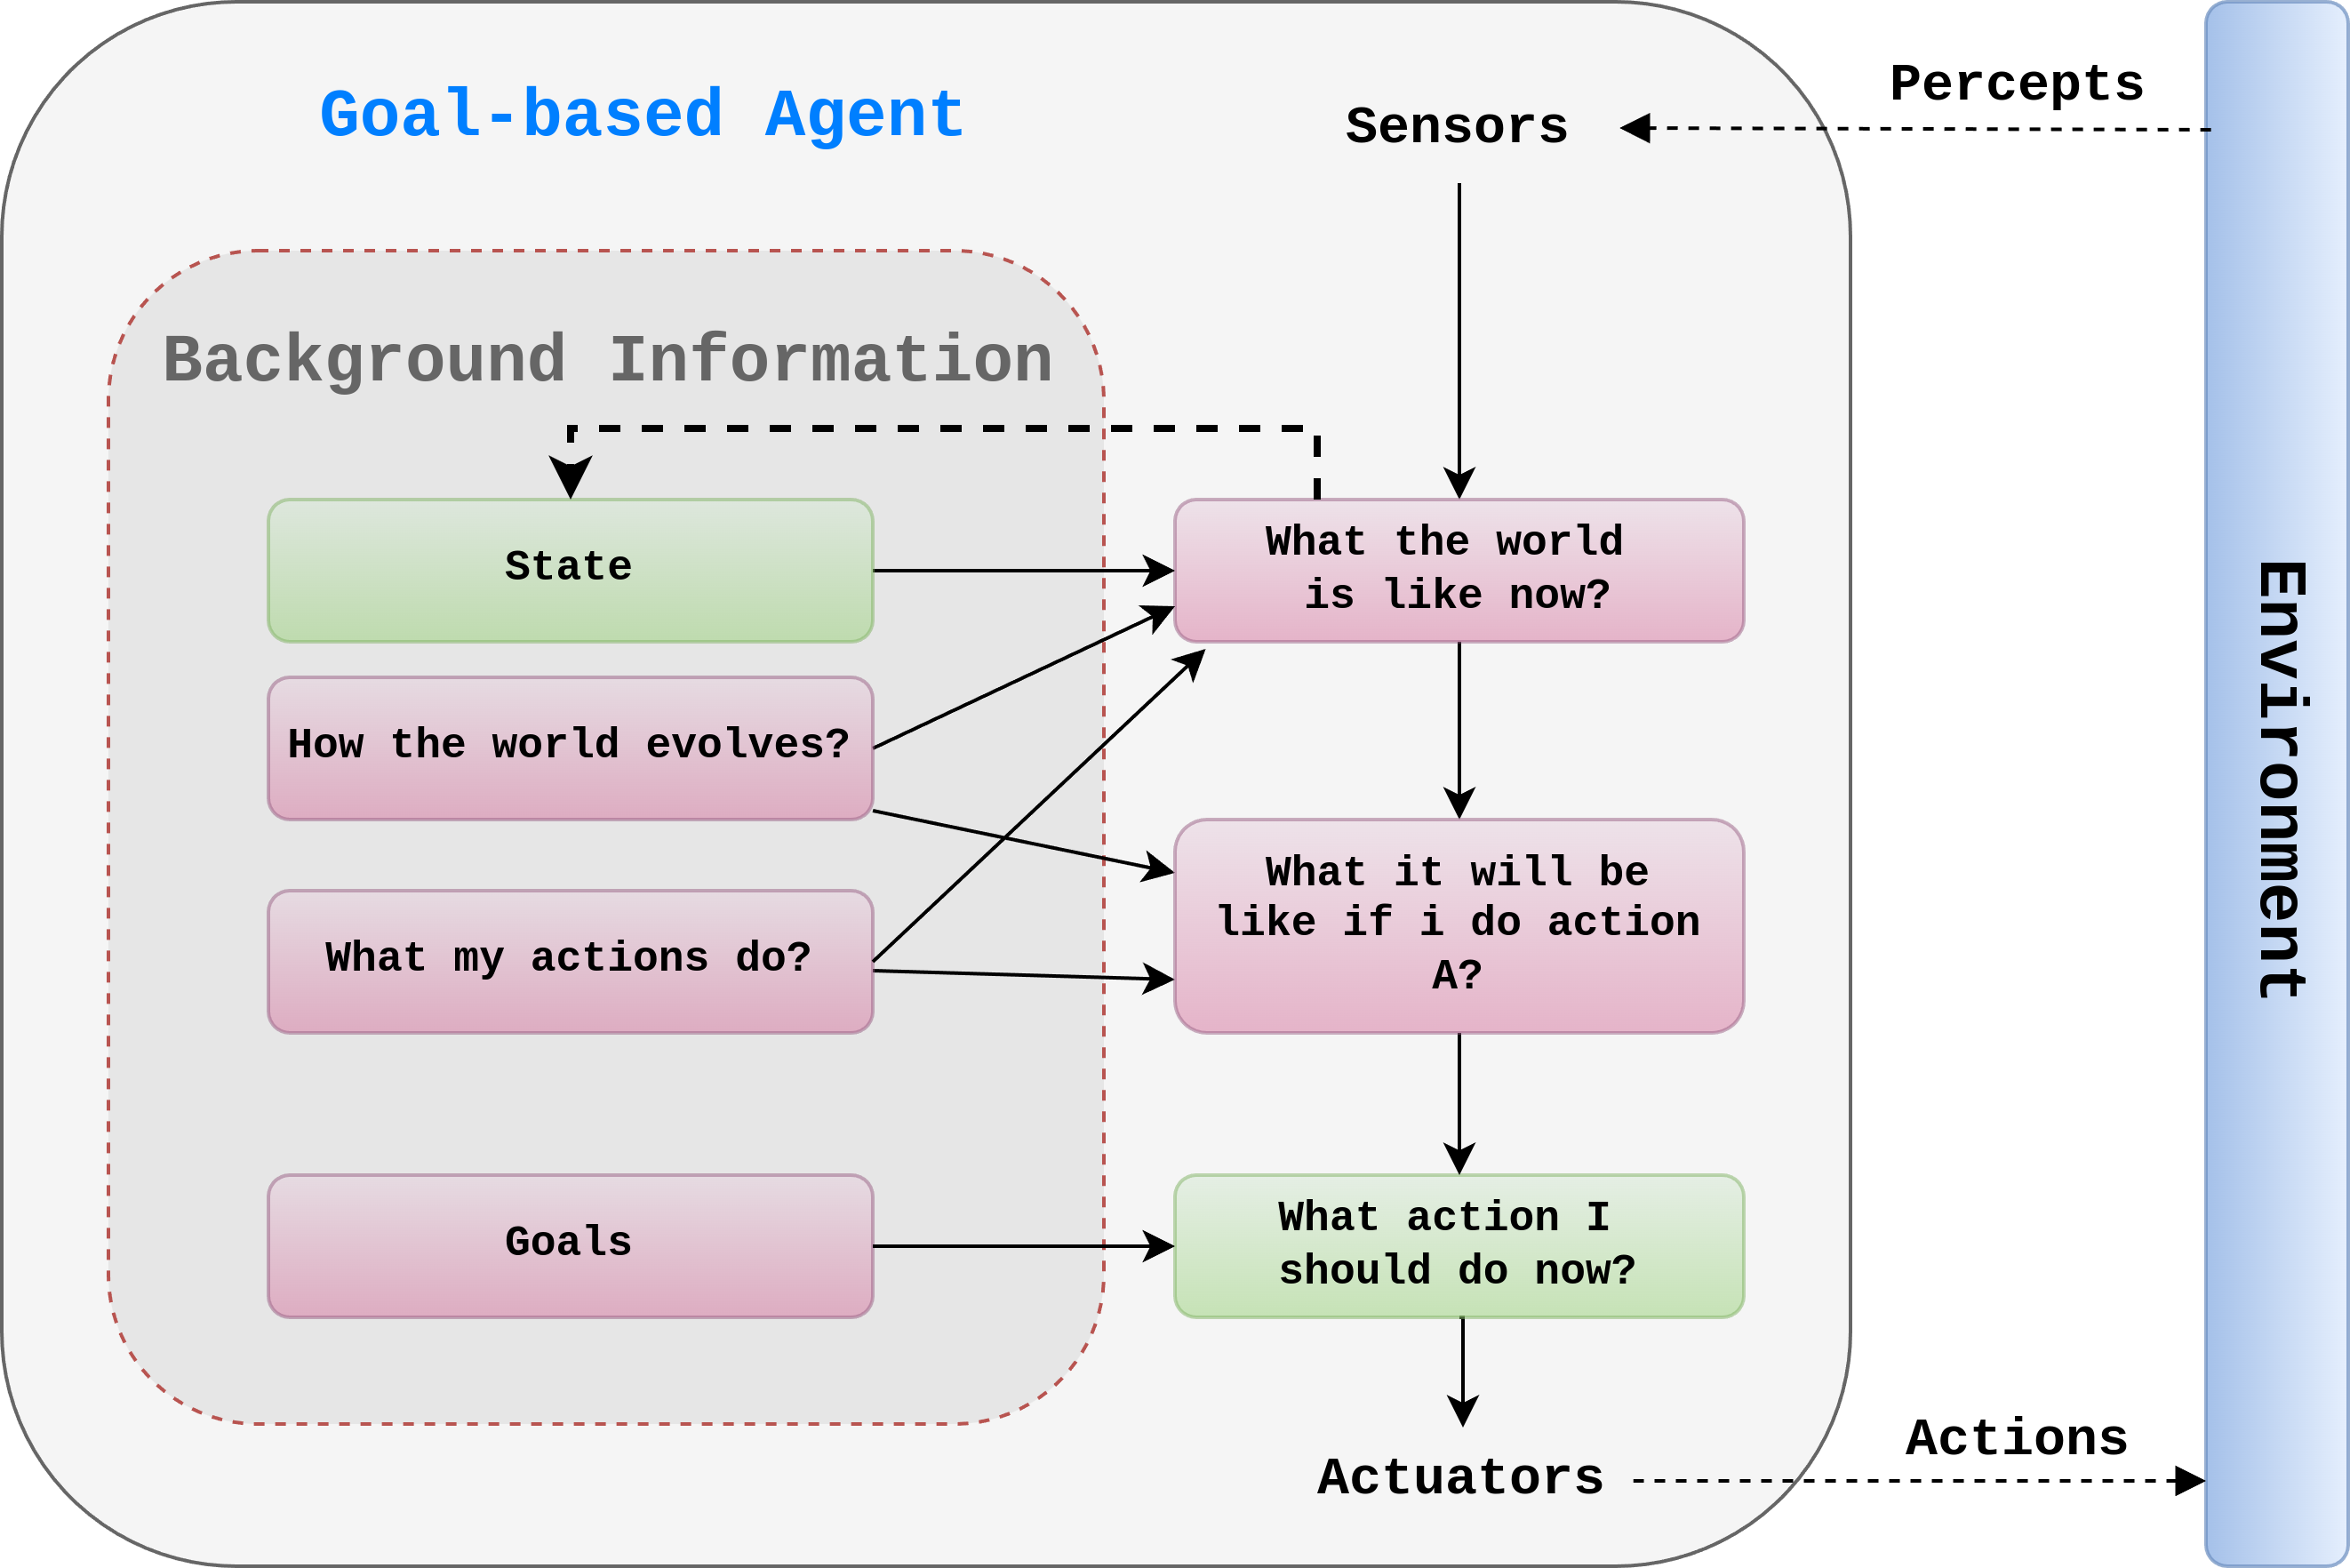
\includegraphics[
        width=0.5\linewidth, 
        height=6cm, 
        keepaspectratio
    ]{images/artificial-intelligence/ai-agents/agents-Goal-based-agent.png}
    \caption*{A model-based, goal-based agent. \cite{common/online/tools/draw.io}}
\end{figure}



\begin{enumerate}[itemsep=0.2cm]
    \item As well as a current state description, the agent needs some sort of \textbf{goal} information that describes situations that are desirable.
    \hfill \cite{ai/book/Artificial-Intelligence-A-Modern-Approach/Russell-Norvig}

    \item  The agent program can combine this with the model (the same information as was used in the modelbased reflex agent) to choose actions that achieve the goal.
    \hfill \cite{ai/book/Artificial-Intelligence-A-Modern-Approach/Russell-Norvig}

    \item Sometimes goal-based action selection is straightforward - for example, when goal satisfaction results immediately from a single action. Sometimes it will be more tricky - for example, when the agent has to consider long sequences of twists and turns in order to find a way to achieve the goal.
    \hfill \cite{ai/book/Artificial-Intelligence-A-Modern-Approach/Russell-Norvig}

    \item decision making of this kind is fundamentally different from the condition–action rules \\
    decision making involves consideration of the future - both \textit{“What will happen if I do such-and-such?”} and \textit{“Will that make me happy?”}.
    \hfill \cite{ai/book/Artificial-Intelligence-A-Modern-Approach/Russell-Norvig}

    \item It is \textbf{not reflexive}. It takes calculated decisions.

    \item Although the goal-based agent appears less efficient, it is more flexible because the knowledge that supports its decisions is represented explicitly and can be modified.
    \hfill \cite{ai/book/Artificial-Intelligence-A-Modern-Approach/Russell-Norvig}

    \item Goals just provide a crude binary distinction between “happy” and “unhappy” states.
    \hfill \cite{ai/book/Artificial-Intelligence-A-Modern-Approach/Russell-Norvig}

    \item SEE: subfields of AI devoted to finding action sequences that achieve the agent’s goals: (TODO)
    \begin{enumerate}
        \item Search
        \item Planning
    \end{enumerate}
\end{enumerate}


\section{(Model-based Goal-based) Utility-based Agents}\label{AI: Agent Programs/(Model-based Goal-based) Utility-based Agents}


\begin{figure}[H]
    \centering
    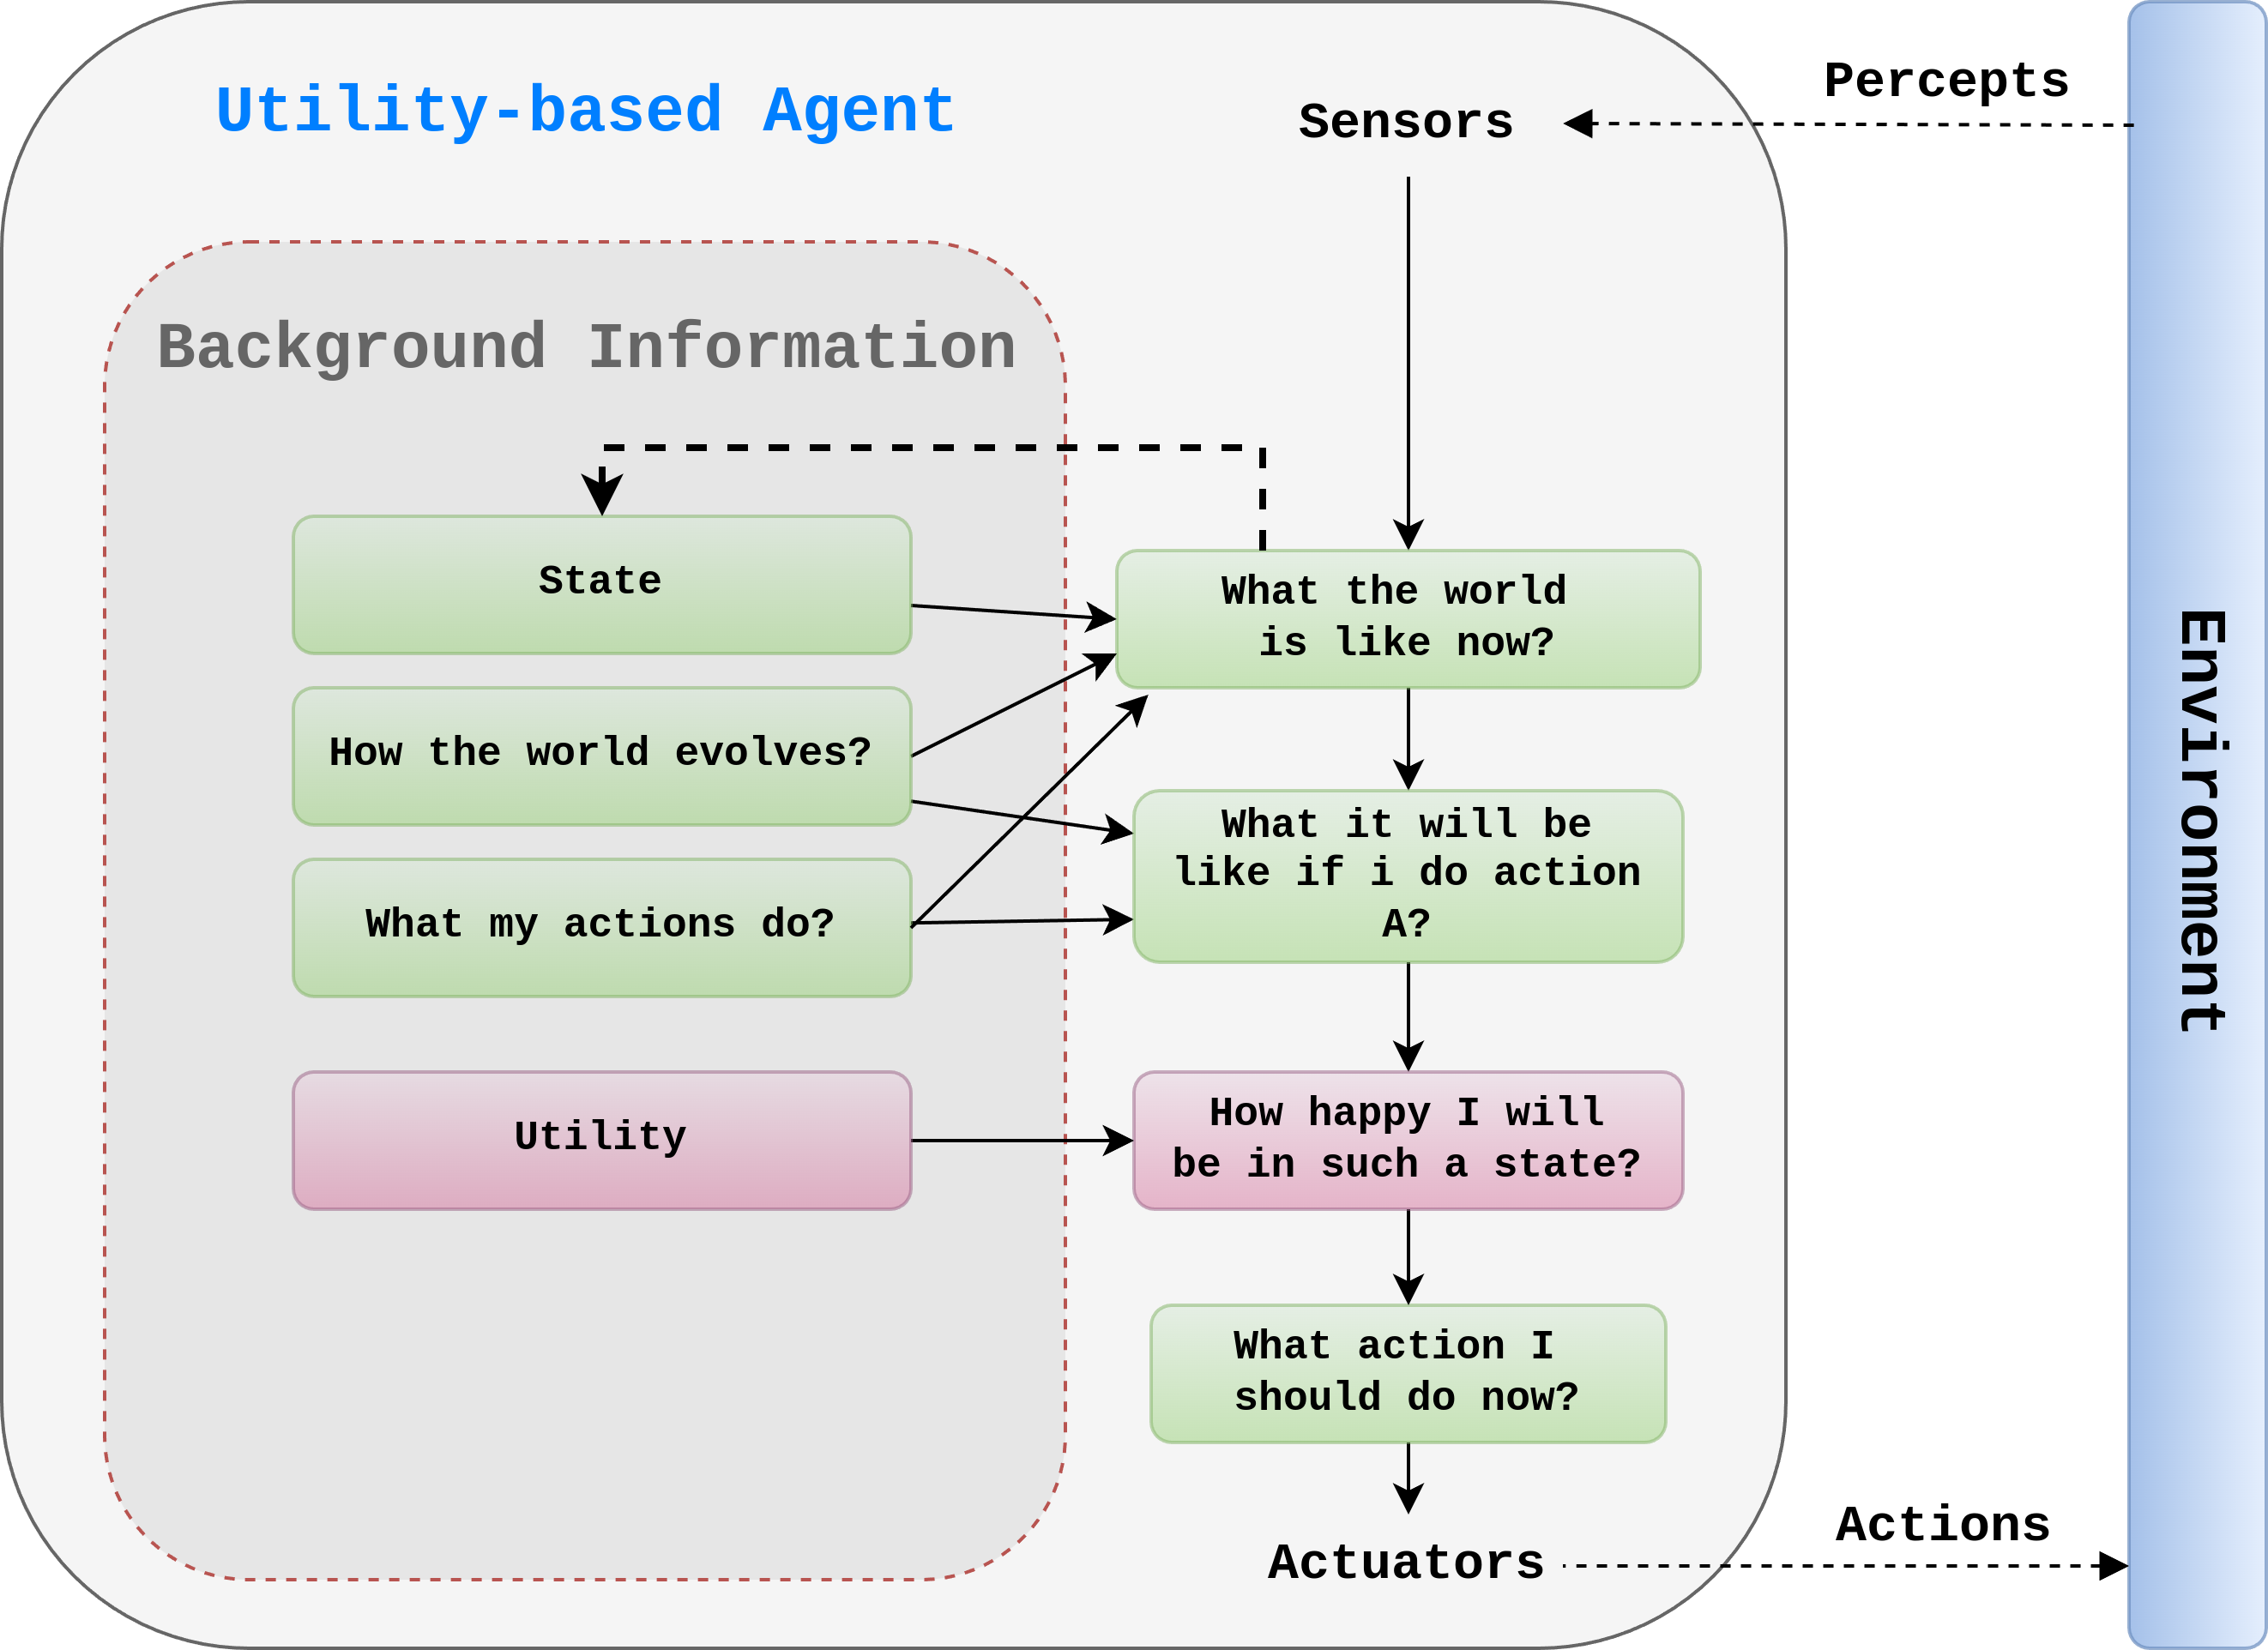
\includegraphics[
        width=0.5\linewidth,
        height=6cm,
        keepaspectratio
    ]{images/artificial-intelligence/ai-agents/agents-utility-based-agent.png}
    \caption*{A model-based, goal-based, utility-based agent. \cite{common/online/tools/draw.io}}
\end{figure}

\hspace{0.5cm}

\begin{enumerate}
    \item A more general performance measure than Goal (happy/ unhappy) should allow a comparison of different world states according to exactly how happy they would make the agent.
    \hfill \cite{ai/book/Artificial-Intelligence-A-Modern-Approach/Russell-Norvig}

    \item An agent’s \textbf{utility function} is essentially an internalization of the performance measure.
    \hfill \cite{ai/book/Artificial-Intelligence-A-Modern-Approach/Russell-Norvig}
    \\
    (The word “utility” here refers to “\textit{the quality of being useful}”)

    \item  If the internal utility function and the external performance measure are in agreement, then an agent that chooses actions to maximize its utility will be rational according to the external performance measure.
    \hfill \cite{ai/book/Artificial-Intelligence-A-Modern-Approach/Russell-Norvig}

    \item this is \textbf{not the only} way to be rational but, like goal-based agents, a utility-based agent has many advantages in terms of flexibility and learning
    \hfill \cite{ai/book/Artificial-Intelligence-A-Modern-Approach/Russell-Norvig}

    \item (\textbf{Advantage}) in two kinds of cases, goals are inadequate but a utility-based agent can still make rational decisions:
    \begin{enumerate}
        \item when there are conflicting goals, only some of which can be achieved (for example, speed and safety), the utility function specifies the appropriate tradeoff
        \hfill \cite{ai/book/Artificial-Intelligence-A-Modern-Approach/Russell-Norvig}

        \item when there are several goals that the agent can aim for, none of which can be achieved with certainty, utility provides a way in which the likelihood of success can be weighed against the importance of the goals.
        \hfill \cite{ai/book/Artificial-Intelligence-A-Modern-Approach/Russell-Norvig}
    \end{enumerate}

    \item Partial observability and stochasticity are ubiquitous in the real world, and so, therefore, is decision making under uncertainty.
    \hfill \cite{ai/book/Artificial-Intelligence-A-Modern-Approach/Russell-Norvig}

    \item a rational utility-based agent chooses the action that maximizes the expected utility of the action outcomes - that is, the utility the agent expects to derive, on average, given the probabilities and utilities of each outcome.
    \hfill \cite{ai/book/Artificial-Intelligence-A-Modern-Approach/Russell-Norvig}

    \item An agent that possesses an explicit utility function can make rational decisions with a general-purpose algorithm that does not depend on the specific utility function being maximized. In this way, the “global” definition of rationality - designating as rational those agent functions that have the highest performance - is turned into a “local” constraint on rational-agent designs that can be expressed in a simple program.
    \hfill \cite{ai/book/Artificial-Intelligence-A-Modern-Approach/Russell-Norvig}

    \item A utility-based agent has to model and keep track of its environment, tasks that have involved a great deal of research on perception, representation, reasoning, and learning.
    \hfill \cite{ai/book/Artificial-Intelligence-A-Modern-Approach/Russell-Norvig}

    \item Choosing the utility-maximizing course of action is also a difficult task, requiring ingenious algorithms.
    \hfill \cite{ai/book/Artificial-Intelligence-A-Modern-Approach/Russell-Norvig}
\end{enumerate}



\vspace{0.5cm}


\begin{customArrayStretch}{1.3}
\begin{table}[H]
\centering

\begin{tabular}{| l | l | l |}

\hline

\textbf{Aspect} &
    \textbf{Utility Function} &
    \textbf{Performance Measure} \\ \hline

\textbf{Perspective} &
    From the agent’s point of view &
    From the external evaluator’s point of view \\ \hline

\textbf{Goal} &
    Maximize expected utility &
    Maximize measurable performance \\ \hline

\textbf{Usage} &
    Guides decision-making &
    Evaluates overall system success \\ \hline

\end{tabular}

\caption*{Utility Function VS Performance Measure}
\end{table}
\end{customArrayStretch}















\section{Learning agents}\label{AI: Agent Programs/Learning agents}

\begin{figure}[H]
    \centering
    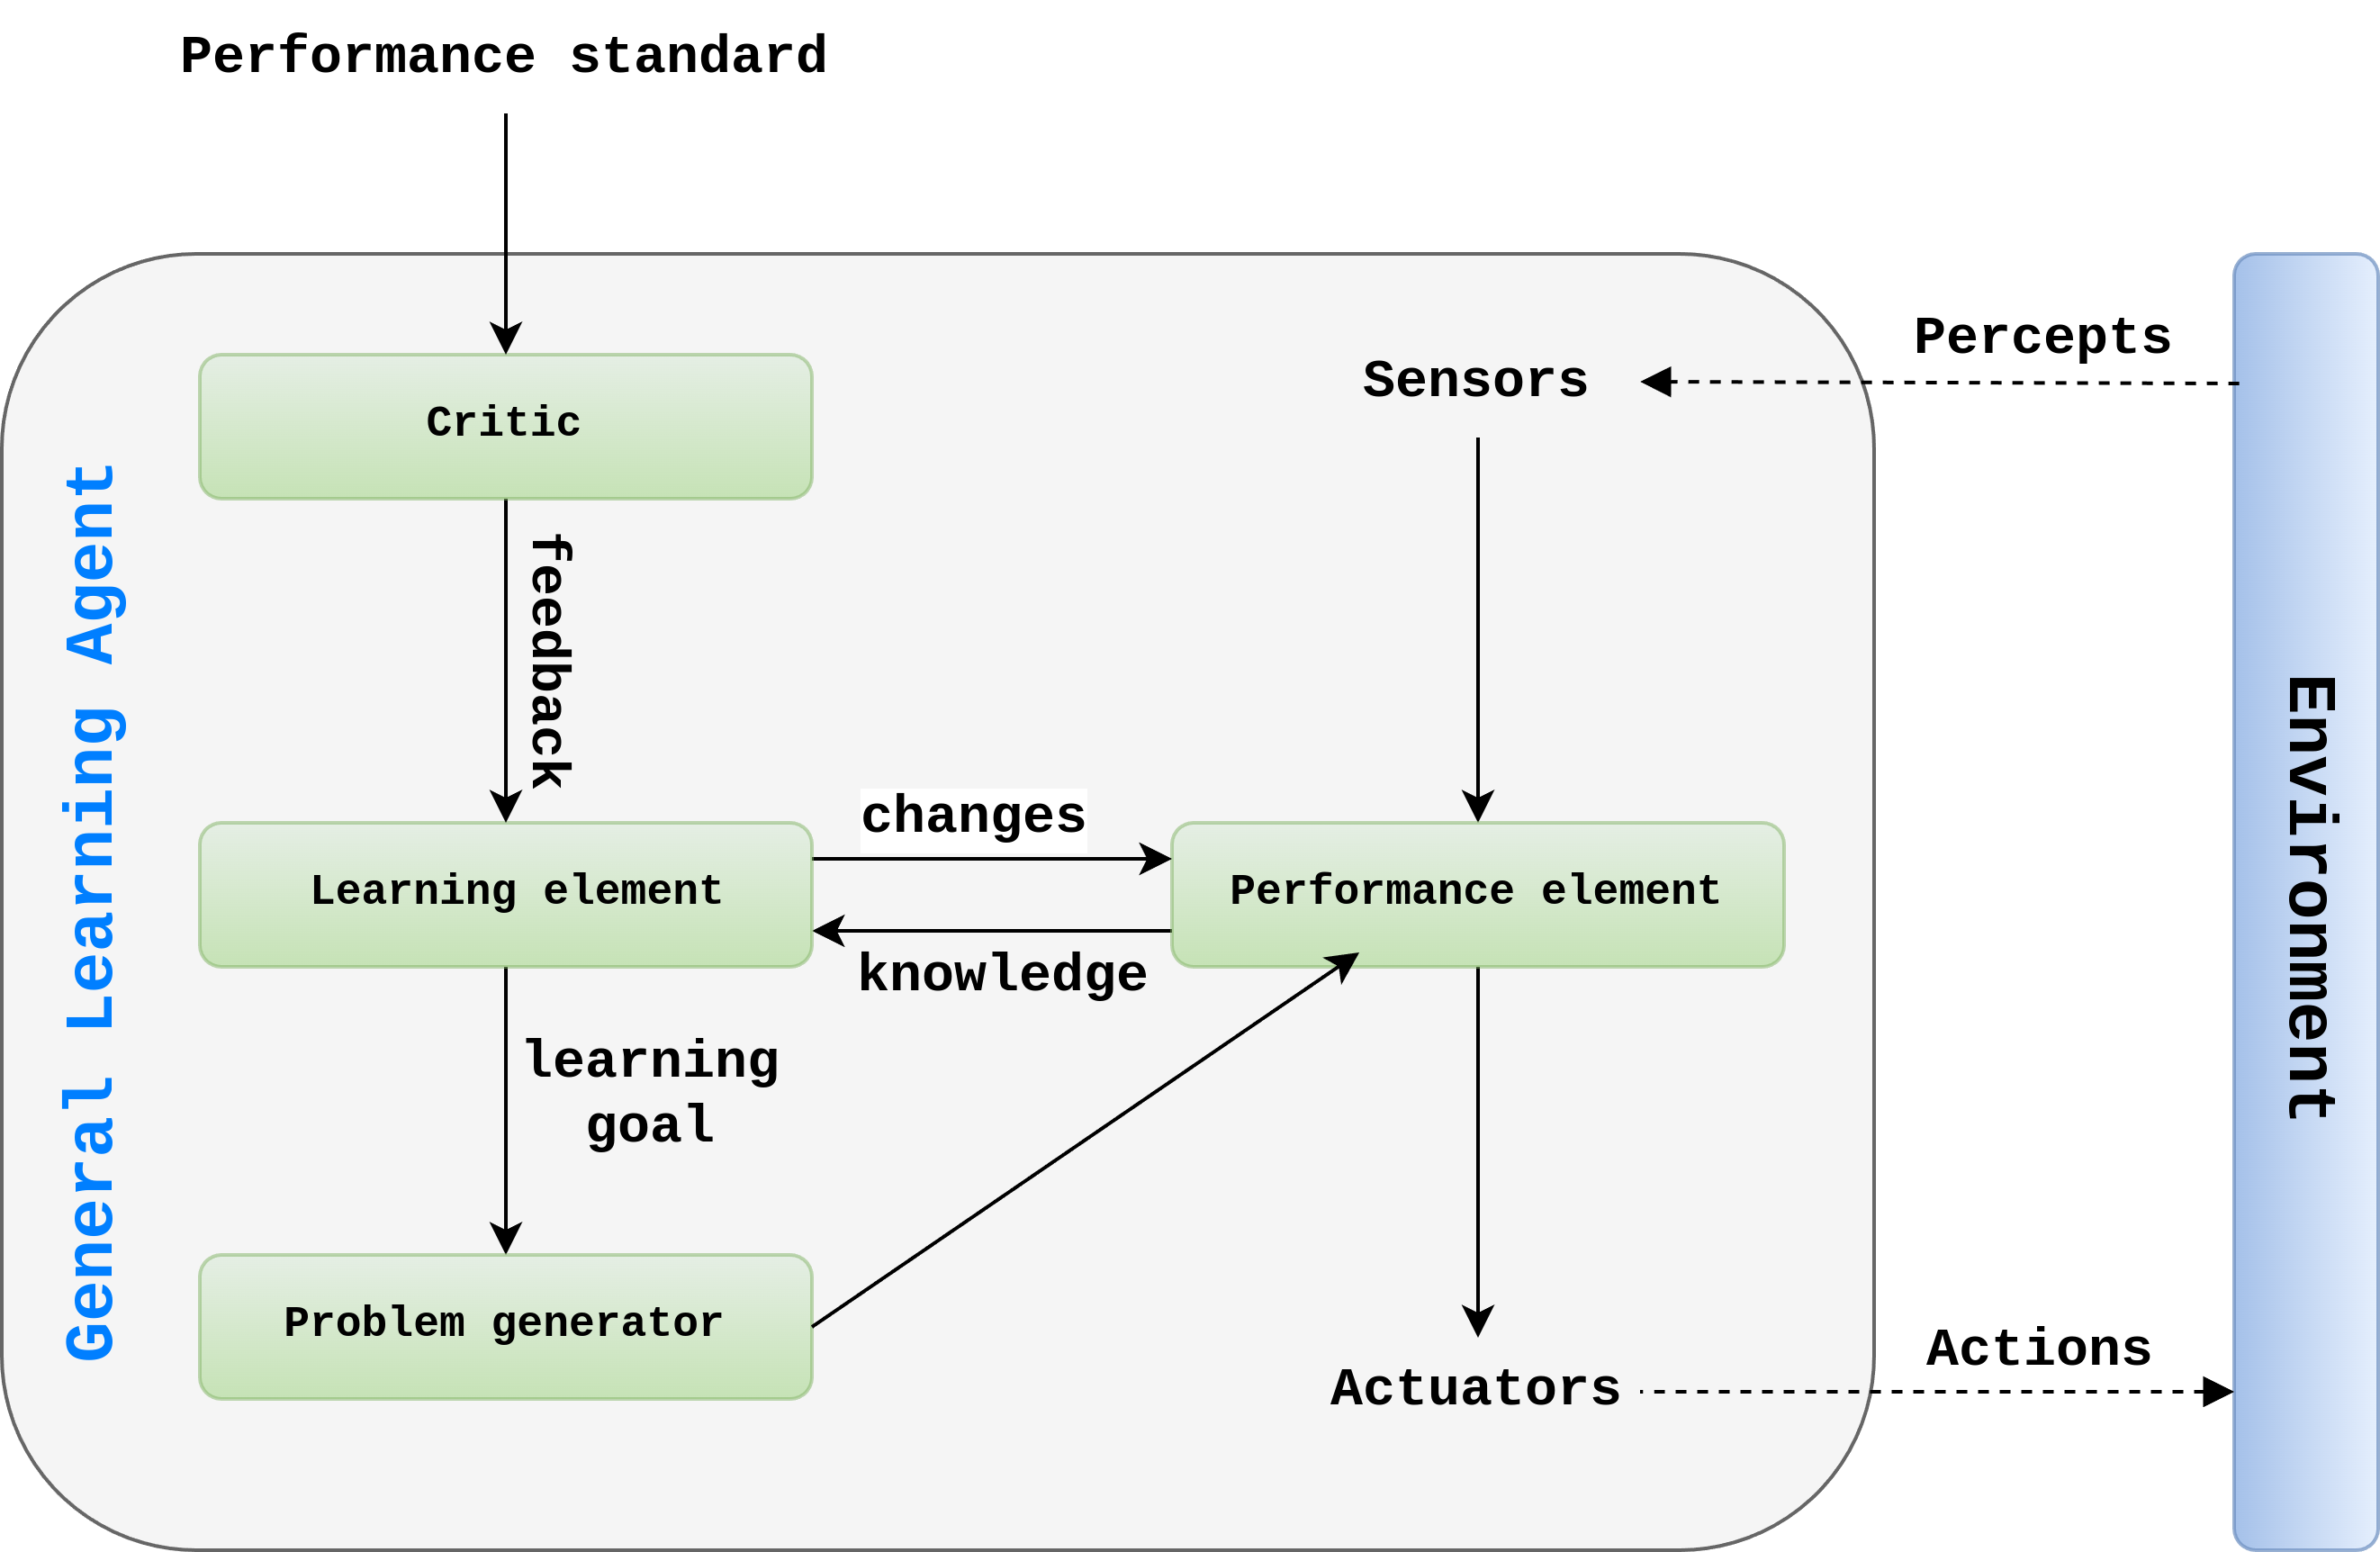
\includegraphics[
        width=0.5\linewidth, 
        height=6cm, 
        keepaspectratio
    ]{images/artificial-intelligence/ai-agents/agents-general-learning-agent.png}
    \caption*{A general learning agent. \cite{common/online/tools/draw.io}}
\end{figure}


\vspace{0.5cm}


\begin{enumerate}[itemsep=0.2cm]
    \item In his famous early paper, \textbf{Turing} (1950) considers the idea of actually programming his intelligent machines by hand.
    \hfill \cite{ai/book/Artificial-Intelligence-A-Modern-Approach/Russell-Norvig}

    \item  \textbf{advantage}: it allows the agent to operate in initially unknown environments and to become more competent than its initial knowledge alone might allow.
    \hfill \cite{ai/book/Artificial-Intelligence-A-Modern-Approach/Russell-Norvig}

    \item \textbf{conceptual components}:
    \begin{enumerate}[itemsep=0.1cm]
        \item \textbf{learning element}: responsible for making improvements
        \hfill \cite{ai/book/Artificial-Intelligence-A-Modern-Approach/Russell-Norvig}

        \item \textbf{performance element}: responsible for selecting external actions. it takes in percepts and decides on actions.
        \hfill \cite{ai/book/Artificial-Intelligence-A-Modern-Approach/Russell-Norvig}
        \\
        The design of the learning element depends very much on the design of the performance element. When trying to design an agent that learns a certain capability, the first question is \textbf{not} “\textit{How am I going to get it to learn this?}” \textbf{but} “\textit{What kind of performance element will my agent need to do this once it has learned how?}”
        \hfill \cite{ai/book/Artificial-Intelligence-A-Modern-Approach/Russell-Norvig}
        \\
        It is important that the performance standard be fixed. Conceptually, one should think of it as being outside the agent altogether because the agent \textbf{must not} modify it to fit its own behavior.
        \hfill \cite{ai/book/Artificial-Intelligence-A-Modern-Approach/Russell-Norvig}

        \item \textbf{critic}: The learning element uses feedback from the critic on how the agent is doing and determines how the performance element should be modified to do better in the future. 
        \hfill \cite{ai/book/Artificial-Intelligence-A-Modern-Approach/Russell-Norvig}
        \\
        The critic tells the learning element how well the agent is doing with respect to a fixed performance standard. The critic is necessary because the percepts themselves provide \textbf{no} indication of the agent’s success.
        \hfill \cite{ai/book/Artificial-Intelligence-A-Modern-Approach/Russell-Norvig}

        \item \textbf{problem generator}: It is responsible for suggesting actions that will lead to new and informative experiences. The point is that if the performance element had its way, it would keep doing the actions that are best, given what it knows. But if the agent is willing to explore a little and do some perhaps suboptimal actions in the short run, it might discover much better actions for the long run. 
        \hfill \cite{ai/book/Artificial-Intelligence-A-Modern-Approach/Russell-Norvig}
        \\
        The problem generator might identify certain areas of behavior in need of improvement and suggest experiments.
        \hfill \cite{ai/book/Artificial-Intelligence-A-Modern-Approach/Russell-Norvig}
         
    \end{enumerate}

    \item The learning element can make changes to any of the “\textit{knowledge}” components in the previous agents(simple reflex, model based, goal based, utility based). The simplest cases involve learning directly from the percept sequence. Observation of pairs of successive states of the environment can allow the agent to learn “How the world evolves,” and observation of the results of its actions can allow the agent to learn “What my actions do.”.
    The forms of learning do not need to access the external performance standard.
    \hfill \cite{ai/book/Artificial-Intelligence-A-Modern-Approach/Russell-Norvig}


    \item In a sense, the \textbf{external performance standard} is the \textit{universal} one of making predictions that agree with experiment.
    \hfill \cite{ai/book/Artificial-Intelligence-A-Modern-Approach/Russell-Norvig}

    \item  In a sense, the performance standard distinguishes part of the incoming percept as a \textbf{reward} (or \textbf{penalty}) that provides direct feedback on the quality of the agent’s behavior. Hard-wired performance standards such as pain and hunger in animals can be understood in this way.
    \hfill \cite{ai/book/Artificial-Intelligence-A-Modern-Approach/Russell-Norvig}

    \item Learning in intelligent agents can be summarized as a process of modification of each component of the agent to bring the components into closer agreement with the available feedback information, thereby improving the overall performance of the agent.
    \hfill \cite{ai/book/Artificial-Intelligence-A-Modern-Approach/Russell-Norvig}

    \item Intelligent agents are supposed to maximize their performance measure.
    \hfill \cite{ai/book/Artificial-Intelligence-A-Modern-Approach/Russell-Norvig}
\end{enumerate}



\section{Problem-Solving Agent}\label{AI: Agent Programs/Problem-Solving Agent}



\begin{enumerate}
    \item one kind of \textit{goal-based agent} that use \textbf{atomic} representations
    \hfill \cite{ai/book/Artificial-Intelligence-A-Modern-Approach/Russell-Norvig}

    \item \textbf{uninformed search algorithms}: algorithms that are given \textbf{no information} about the problem other than its definition
    \hfill \cite{ai/book/Artificial-Intelligence-A-Modern-Approach/Russell-Norvig}
    \\
    some of these algorithms can solve any solvable problem, none of them can do so efficiently
    \hfill \cite{ai/book/Artificial-Intelligence-A-Modern-Approach/Russell-Norvig}

    \item \textbf{Informed search algorithms}: can do quite well given some guidance on where to look for solutions.
    \hfill \cite{ai/book/Artificial-Intelligence-A-Modern-Approach/Russell-Norvig}

    \item \textbf{Goal formulation}, based on the current situation and the agent’s performance measure, is the first step in problem solving.
    \hfill \cite{ai/book/Artificial-Intelligence-A-Modern-Approach/Russell-Norvig}

    \item We consider a goal to be a set of world states—exactly those states in which the goal is satisfied.
    The agent’s task is to find out how to act, now and in the future, so that it reaches a goal state.
    \hfill \cite{ai/book/Artificial-Intelligence-A-Modern-Approach/Russell-Norvig}

\subsection*{Simple “formulate, search, execute” design}

    \item \textbf{Problem formulation} is the process of deciding what actions and states to consider, given a goal.
    \hfill \cite{ai/book/Artificial-Intelligence-A-Modern-Approach/Russell-Norvig}

    \item An agent with several immediate options of unknown value can decide what to do by first examining future actions that eventually lead to states of known value.
    \hfill \cite{ai/book/Artificial-Intelligence-A-Modern-Approach/Russell-Norvig}

    \item The process of looking for a sequence of actions that reaches the goal is called \textbf{search}.
    \hfill \cite{ai/book/Artificial-Intelligence-A-Modern-Approach/Russell-Norvig}

    \item A \textit{search algorithm} takes a problem as input and returns a \textbf{solution} in the form of an action sequence.
    \hfill \cite{ai/book/Artificial-Intelligence-A-Modern-Approach/Russell-Norvig}

    \item Once a solution is found, the actions it recommends can be carried out. This is called the \textbf{execution} phase.
    While the agent is executing the solution sequence it \textit{ignores} its percepts when choosing an action because it knows in advance what they will be.
    \hfill \cite{ai/book/Artificial-Intelligence-A-Modern-Approach/Russell-Norvig}

    \item Once the solution has been executed, the agent will formulate a new goal.
    \hfill \cite{ai/book/Artificial-Intelligence-A-Modern-Approach/Russell-Norvig}

    \item An agent that carries out its plans with its eyes closed, so to speak, must be quite certain of what is going on. Control theorists call this an \textbf{open-loop system}, because ignoring the percepts breaks the loop between agent and environment.
    \hfill \cite{ai/book/Artificial-Intelligence-A-Modern-Approach/Russell-Norvig}
\end{enumerate}








\vspace{0.5cm}


\begin{algorithm}[H]
    \caption{A simple problem-solving agent. It first formulates a goal and a problem, searches for a sequence of actions that would solve the problem, and then executes the actions one at a time. When this is complete, it formulates another goal and starts over \cite{ai/book/Artificial-Intelligence-A-Modern-Approach/Russell-Norvig}}

    \SetKwFunction{FUNCTION}{\textsc{Simple-Problem-Solving-Agent}}
    \SetKwProg{Fn}{function}{ returns \normalfont an action}{end}
    \Fn{\FUNCTION{ percept }}{
        \textbf{persistent}:\\
            \hspace{1cm} $seq$, an action sequence, initially empty \\
            \hspace{1cm} $state$, some description of the current world state \\
            \hspace{1cm} $goal$, a goal, initially null \\
            \hspace{1cm} $problem$, a problem formulation \\
        \ \\
        $state$ $\gets$ \textsc{Update-State}( $state,\ percept$ )

        \If{$seq$ \normalfont is empty}{
            $goal$ $\gets$ \textsc{Formulate-Goal}( $state$ ) \\
            $problem$ $\gets$ \textsc{Formulate-Problem}( $state,\ goal$ )\\
            $seq$ $\gets$ \textsc{Search}( $prolem$ ) \\

            \If{$seq\ = \ failure$ }{
                \Return a null action
            }
        }

        $action$ $\gets$ \textsc{First}( $seq$ )\\
        $seq$ $\gets$ \textsc{Rest}( $seq$ )

        \Return $action$
    }
\end{algorithm}



\subsection{Defining \& Formulating Problem}

\begin{enumerate}
    \item The \textbf{initial state} that the agent starts in.
    \hfill \cite{ai/book/Artificial-Intelligence-A-Modern-Approach/Russell-Norvig}

    \item A description of the possible \textbf{actions} available to the agent. Given a particular state $s$, \textsc{Actions}($s$) returns the set of actions that can be executed in $s$. We say that each of these actions is \textit{applicable} in $s$.
    \hfill \cite{ai/book/Artificial-Intelligence-A-Modern-Approach/Russell-Norvig}

    \item A description of what each action does; the formal name for this is the \textbf{transition model}, specified by a function \textsc{Result}($s,\ a$) that returns the state that results from  doing action $a$ in state $s$.
    We also use the term \textbf{successor} to refer to any state reachable from a given state by a single action.
    \hfill \cite{ai/book/Artificial-Intelligence-A-Modern-Approach/Russell-Norvig}

    \item The \textbf{goal test}, which determines whether a given state is a goal state.
    Sometimes there is an \textit{explicit} set of possible goal states, and the test simply checks whether the given state is one of them.
    Sometimes the goal is specified by an \textit{abstract property} rather than an explicitly enumerated set of states.
    \hfill \cite{ai/book/Artificial-Intelligence-A-Modern-Approach/Russell-Norvig}

    \item A \textbf{path cost} function that assigns a numeric cost to each path. The problem-solving agent chooses a cost function that reflects its own performance measure.
    We assume that the cost of a path can be described as the \textit{sum} of the costs of the individual actions along the path.
    \hfill \cite{ai/book/Artificial-Intelligence-A-Modern-Approach/Russell-Norvig}
\end{enumerate}

\vspace{0.5cm}

\textbf{Note}:

\begin{enumerate}
    \item Together, the initial state, actions, and transition model implicitly define the \textbf{state space} of the problem—the set of all states reachable from the initial state by any sequence of actions. The state space forms a directed network or \textbf{graph} in which the nodes are states and the links between nodes are actions.
    \hfill \cite{ai/book/Artificial-Intelligence-A-Modern-Approach/Russell-Norvig}

    \item \textbf{diameter of the state space}: The maximum number of steps (or actions) required to go from any one state to any other reachable state in the state space.
    \hfill \cite{ai/book/Artificial-Intelligence-A-Modern-Approach/Russell-Norvig}

    \item A \textbf{path} in the state space is a sequence of states connected by a sequence of actions.
    \hfill \cite{ai/book/Artificial-Intelligence-A-Modern-Approach/Russell-Norvig}

    \item The \textbf{step cost} of taking action $a$ in state $s$ to reach state $s^\prime$ is denoted by $c(s,\ a,\ s^\prime)$.
    \hfill \cite{ai/book/Artificial-Intelligence-A-Modern-Approach/Russell-Norvig}

    \item A \textbf{solution} to a problem is an \textit{action sequence} that leads from the initial state to a goal state.
    \hfill \cite{ai/book/Artificial-Intelligence-A-Modern-Approach/Russell-Norvig}

    \item Solution quality is measured by the path cost function, and an \textbf{optimal solution} has the lowest path cost among all solutions.
    \hfill \cite{ai/book/Artificial-Intelligence-A-Modern-Approach/Russell-Norvig}

    \item In addition to abstracting the state description, we must abstract the actions themselves.
    \hfill \cite{ai/book/Artificial-Intelligence-A-Modern-Approach/Russell-Norvig}

    \item The abstraction is \textbf{valid} if we can expand any abstract solution into a solution in the more detailed world
    \hfill \cite{ai/book/Artificial-Intelligence-A-Modern-Approach/Russell-Norvig}

    \item The abstraction is \textbf{useful} if carrying out each of the actions in the solution is easier than the original problem
    \hfill \cite{ai/book/Artificial-Intelligence-A-Modern-Approach/Russell-Norvig}

    \item \textbf{meta-level state space}: Each \textbfit{state} in a meta-level state space captures the internal (computational) state of a program that is searching in an \textbf{object-level state space}.
    Each \textbfit{action} in the meta-level state space is a computation step that alters the internal state.
    A sequence of larger and larger search trees, can be seen as depicting a path in the meta-level state space where each state on the path is an object-level search tree
    \hfill \cite{ai/book/Artificial-Intelligence-A-Modern-Approach/Russell-Norvig}
    \\
    \textbf{Example}: the internal state of the A$^\ast$ algorithm consists of the current search tree.
    each computation step in A$^\ast$ expands a leaf node and adds its successors to the tree
    \hfill \cite{ai/book/Artificial-Intelligence-A-Modern-Approach/Russell-Norvig}

    \item \textbf{meta-level learning algorithm} can learn from experiences (missteps in harder problems) to avoid exploring unpromising sub-trees.
    The goal of learning is to \textit{minimize} the \textbf{total cost} of problem solving, trading off computational expense and path cost.
    \hfill \cite{ai/book/Artificial-Intelligence-A-Modern-Approach/Russell-Norvig}

    \item \textbf{relaxed problem}: A problem with \textit{fewer restrictions} on the actions
    \hfill \cite{ai/book/Artificial-Intelligence-A-Modern-Approach/Russell-Norvig}
    \\
    The state-space graph of the relaxed problem is a \textbf{super-graph} of the original state space because the removal of restrictions creates added edges in the graph.
    \hfill \cite{ai/book/Artificial-Intelligence-A-Modern-Approach/Russell-Norvig}
    \\
    Because the relaxed problem adds edges to the state space, any optimal solution in the original problem is, by definition, also a solution in the relaxed problem; but the relaxed problem may have \textbf{better solutions} if the added edges provide \textbf{short cuts}. Hence, \textbfit{the cost of an optimal solution to a relaxed problem is an admissible heuristic for the original problem}.
    \hfill \cite{ai/book/Artificial-Intelligence-A-Modern-Approach/Russell-Norvig}
    \\
    because the derived heuristic is an exact cost for the relaxed problem, it must obey the triangle inequality and is therefore \textbf{consistent}
    \hfill \cite{ai/book/Artificial-Intelligence-A-Modern-Approach/Russell-Norvig}

    \item  it is crucial that the relaxed problems generated by this technique can be solved essentially \textbf{without search}, because the relaxed rules allow the problem to be decomposed into some independent subproblems.
    If the relaxed problem is hard to solve, then the values of the corresponding heuristic will be \textbf{expensive} to obtain.
    \hfill \cite{ai/book/Artificial-Intelligence-A-Modern-Approach/Russell-Norvig}
\end{enumerate}

\vspace{0.2cm}

\begin{lstlisting}[
    language=Python,
    caption=Problem Solving Agent - Problem Skeleton
]
class Problem:
    def __init__(self, initial_state: State):
        self.initial_state = initial_state
        # 1. initial_state: The initial state that the agent starts in.

    def actions(self, state: State):
        """
            2. A description of the possible actions available to the agent.
            Given a particular state s, ACTIONS(s) returns the set of actions
            that can be executed in s.
        """
        raise NotImplementedError()

    def result(self, state: State, action):
        """
            3. A description of what each action does; the formal name for this
            is the transition model, specified by a function RESULT(s, a) that
            returns the state that results from doing action a in state s.
        """
        raise NotImplementedError()

    def goal_test(self, state: State):
        # 4. The goal test, which determines whether a given state is a goal state.
        raise NotImplementedError()

    def step_cost(self, state: State, action, new_state: State):
        """
            5. The step cost of taking action
            a in state s to reach state s' is denoted by c(s, a, s').
        """
        raise NotImplementedError()

    def heuristic(self, state: State):
        """
            Returns estimated cost from state to goal.
        """
        raise NotImplementedError()
\end{lstlisting}



\subsection{Measuring problem-solving performance}

\begin{enumerate}
    \item \textbf{Completeness}: Is the algorithm guaranteed to find a solution when there is one?
    \hfill \cite{ai/book/Artificial-Intelligence-A-Modern-Approach/Russell-Norvig}

    \item \textbf{Optimality}: Does the strategy find the optimal solution?
    \hfill \cite{ai/book/Artificial-Intelligence-A-Modern-Approach/Russell-Norvig}

    \item \textbf{Time complexity}: How long does it take to find a solution?
    \hfill \cite{ai/book/Artificial-Intelligence-A-Modern-Approach/Russell-Norvig}

    \item \textbf{Space complexity}: How much memory is needed to perform the search?
    \hfill \cite{ai/book/Artificial-Intelligence-A-Modern-Approach/Russell-Norvig}
\end{enumerate}


\vspace{0.5cm}

\begin{customArrayStretch}{1.3}
\begin{table}[H]
\centering
\begin{tabular}{l l p{12cm}}

$V$ & set & set of vertices (nodes) of the graph \\

$E$ & set & set of edges (links) of the graph \\

$b$ & $\in \mbbR$ & \textbf{branching factor} or maximum number of successors of any node \\

$d$ & $\in \mbbR$ & \textbf{depth} of the \textbf{shallowest goal} node (i.e., the number of steps along the path from the root) \\

$m$ & $\in \mbbR$ & maximum length of any path in the state space \\

\end{tabular}
\caption*{Notations}
\end{table}
\end{customArrayStretch}


\textbf{Note}:
\begin{enumerate}
    \item the typical measure is the \textbf{size} of the \textbf{state space graph}: $|V| + |E|$
    \hfill \cite{ai/book/Artificial-Intelligence-A-Modern-Approach/Russell-Norvig}

    \item Time is often measured in terms of the number of nodes generated during the search, and space in terms of the maximum number of nodes stored in memory.
    \hfill \cite{ai/book/Artificial-Intelligence-A-Modern-Approach/Russell-Norvig}

    \item \textbf{effectiveness of a search algorithm}:
    \begin{enumerate}
        \item \textbf{search cost}: depends on the time complexity but can also include a term for memory usage
        \hfill \cite{ai/book/Artificial-Intelligence-A-Modern-Approach/Russell-Norvig}

        \item \textbf{total cost}: combines the search cost and the path cost of the solution found
        \hfill \cite{ai/book/Artificial-Intelligence-A-Modern-Approach/Russell-Norvig}
    \end{enumerate}

    \item In general, exponential-complexity search problems \textbf{cannot be solved} by uninformed methods for any but the smallest instances.
\end{enumerate}







\section{Planning Agents}\label{AI: Agent Programs/Planning Agents}


\begin{enumerate}[itemsep=0.2cm]
    \item One kind of \textit{goal-based agents} that use more advanced \textbf{factored} or \textbf{structured} representations
    \hfill \cite{ai/book/Artificial-Intelligence-A-Modern-Approach/Russell-Norvig}



\end{enumerate}

















\section{Examples}
\subsection{Vacuum Cleaner \cite{ai/book/Artificial-Intelligence-A-Modern-Approach/Russell-Norvig}}


\begin{figure}[H]
    \centering
    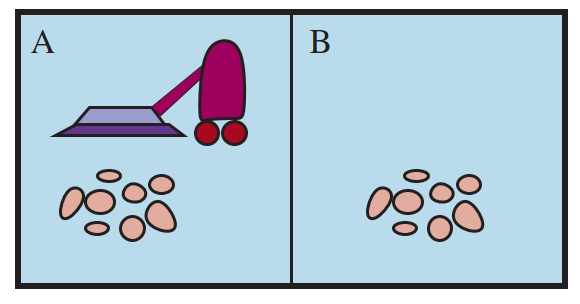
\includegraphics[
        width=0.5\linewidth
    ]{images/artificial-intelligence/examples/example-vacuum-cleaner-world.png}
    \caption*{A vacuum-cleaner world with just two locations}
\end{figure}


\vspace{0.5cm}

\begin{enumerate}[itemsep=0.2cm]
    \item it’s a made-up world

    \item This particular world has just two locations: squares A and B. 
    
    \item The vacuum agent perceives which square it is in and whether there is dirt in the square. 
    
    \item It can choose to \textbf{move left}, \textbf{move right}, \textbf{suck up the dirt}, or \textbf{do nothing}.

    \item One very simple agent function is the following: if the current square is dirty, then suck; otherwise, move to the other square.

    
\end{enumerate}



\subsubsection{As a table driven agent}

\begin{customArrayStretch}{1.3}
\begin{longtable}{|l|l|}

\hline
\textbf{Percept sequence} & \textbf{Action} \\ \hline
\endhead

\hline
\textbf{Percept sequence} & \textbf{Action} \\ \hline
\endfirsthead

\hline\endfoot
\hline\endlastfoot


$[A, \ Clean]$ & $Right$ \\ 
$[A, \ Dirty]$ & $Suck$ \\ 
$[B, \ Clean]$ & $Left$ \\ 
$[B, \ Dirty]$ & $Suck$ \\ 

\vdots & \vdots \\

$[A, \ Clean],\ [A, \ Clean]$ & $Right$ \\ 
$[A, \ Clean],\ [A, \ Dirty]$ & $Suck$ \\ 

\vdots & \vdots \\

$[A, \ Clean],\ [A, \ Clean],\ [A, \ Clean]$ & $Right$ \\ 
$[A, \ Clean],\ [A, \ Clean],\ [A, \ Dirty]$ & $Suck$ \\ 

\vdots & \vdots \\

\end{longtable}
\end{customArrayStretch}





\subsubsection{As a simple reflex agent}

\begin{algorithm}[H]
    \caption{The agent program for a simple reflex agent in the two-state vacuum environment.  \cite{ai/book/Artificial-Intelligence-A-Modern-Approach/Russell-Norvig}}

    \SetKwFunction{FUNCTION}{\textsc{Reflex-Vacuum-Agent}}
    \SetKwProg{Fn}{function}{ returns \normalfont{an action}}{end}
    \Fn{\FUNCTION{[location, status]}}{
        \textbf{if} $status \ = \ Dirty$ \textbf{then return} $Suck$ \\

        \textbf{else if} $location \ = \ A$ \textbf{then return} $Right$ \\

        \textbf{else if} $location \ = \ B$ \textbf{then return} $Left$ \\
    }
\end{algorithm}
















\subsection{Automated Taxi Driver \cite{ai/book/Artificial-Intelligence-A-Modern-Approach/Russell-Norvig}}

\begin{enumerate}[itemsep=0.2cm]
    \item \textbf{Performance Measure}: Safe, fast, legal, comfortable trip, maximize profits
    \hfill \cite{ai/book/Artificial-Intelligence-A-Modern-Approach/Russell-Norvig}

    \item \textbf{Environment}: Roads, other traffic, pedestrians, customers
    \hfill \cite{ai/book/Artificial-Intelligence-A-Modern-Approach/Russell-Norvig}

    \item \textbf{Actuators}: Steering, accelerator, brake, signal, horn, display
    \hfill \cite{ai/book/Artificial-Intelligence-A-Modern-Approach/Russell-Norvig}

    \item \textbf{Sensors}: Cameras, sonar, speedometer, GPS, odometer, accelerometer, engine sensors, keyboard
    \hfill \cite{ai/book/Artificial-Intelligence-A-Modern-Approach/Russell-Norvig}

    \item an automated taxi cannot see what other drivers are thinking.
    \hfill \cite{ai/book/Artificial-Intelligence-A-Modern-Approach/Russell-Norvig}

    \item partially cooperative multiagent environment: avoiding collisions maximizes the performance measure of all agents
    \hfill \cite{ai/book/Artificial-Intelligence-A-Modern-Approach/Russell-Norvig}

    \item \textbf{Task Environment}: partially observable, multiagent, stochastic, sequential, dynamic, continuous, and unknown
    \hfill \cite{ai/book/Artificial-Intelligence-A-Modern-Approach/Russell-Norvig}
    
\end{enumerate}



\subsubsection{As a table driven reflex agent}

\begin{enumerate}[itemsep=0.2cm]
    \item the visual input from a single camera comes in at the rate of roughly $27$ megabytes per second ($30$ frames per second, $640 \times 480$ pixels with $24$-bits of color information). 
    \hfill \cite{ai/book/Artificial-Intelligence-A-Modern-Approach/Russell-Norvig}
    
    \item This gives a lookup table with over $10^{250,000,000,000}$ entries for \textbf{an hour}’s driving.
    \hfill \cite{ai/book/Artificial-Intelligence-A-Modern-Approach/Russell-Norvig}

    \item \textbf{Not possible} to construct the table
    \hfill \cite{ai/book/Artificial-Intelligence-A-Modern-Approach/Russell-Norvig}
\end{enumerate}



\subsubsection{As model-based reflex agents}

\begin{enumerate}[itemsep=0.2cm]
    \item the taxi may be driving back home, and it may have a rule telling it to fill up with gas on the way home unless it has at least half a tank. 
    \hfill \cite{ai/book/Artificial-Intelligence-A-Modern-Approach/Russell-Norvig}
    
    \item Although “driving back home” may seem to an aspect of the world state, the fact of the taxi’s destination is actually an aspect of the agent’s internal state. 
    \hfill \cite{ai/book/Artificial-Intelligence-A-Modern-Approach/Russell-Norvig}
    
    \item If you find this puzzling, consider that the taxi could be in exactly the same place at the same time, but intending to reach a different destination.
    \hfill \cite{ai/book/Artificial-Intelligence-A-Modern-Approach/Russell-Norvig}
    
\end{enumerate}


\subsubsection{As utility-based agents}

\begin{enumerate}[itemsep=0.2cm]
    \item \textbf{utility measures}: quicker, safer, more reliable, or cheaper 
    \hfill \cite{ai/book/Artificial-Intelligence-A-Modern-Approach/Russell-Norvig}
\end{enumerate}


\subsubsection{As Learning Agent}

\begin{enumerate}[itemsep=0.2cm]
    \item The performance element consists of whatever collection of knowledge and procedures the taxi has for selecting its driving actions.
    \hfill \cite{ai/book/Artificial-Intelligence-A-Modern-Approach/Russell-Norvig}

    \item  after the taxi makes a quick left turn across three lanes of traffic, the critic observes the shocking language used by other drivers.
    \hfill \cite{ai/book/Artificial-Intelligence-A-Modern-Approach/Russell-Norvig}

    \item From this experience, the learning element is able to formulate a rule saying this was a bad action, and the performance element is modified by installation of the new rule. 
    \hfill \cite{ai/book/Artificial-Intelligence-A-Modern-Approach/Russell-Norvig}

    
\end{enumerate}










\subsection{Road trip in Romania \cite{ai/book/Artificial-Intelligence-A-Modern-Approach/Russell-Norvig}}


\begin{figure}[H]
    \centering
    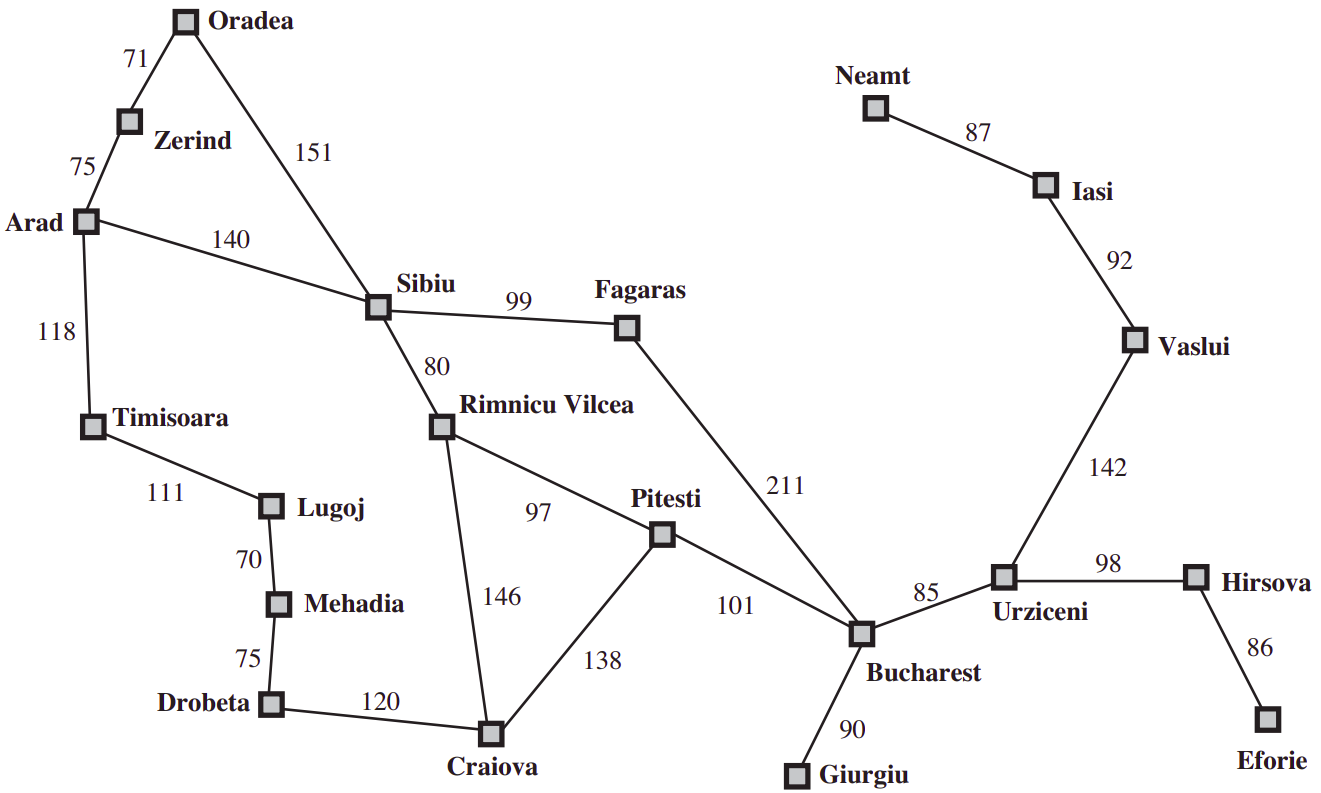
\includegraphics[
        width=\linewidth,
        height=6cm,
        keepaspectratio,
    ]{images/artificial-intelligence/examples/example-romania.png}
    \caption*{A simplified road map of part of Romania. \cite{ai/book/Artificial-Intelligence-A-Modern-Approach/Russell-Norvig}}
\end{figure}



































\chapter{AI: Searching Solutions}


\begin{enumerate}
    \item A solution is an action sequence, so search algorithms work by considering various possible action sequences.
    \hfill \cite{ai/book/Artificial-Intelligence-A-Modern-Approach/Russell-Norvig}

    \item The possible action sequences starting at the initial state form a \textbf{search tree} with the initial state at the root; the branches are actions and the \textbf{nodes} correspond to states in the state space of the problem.
    \hfill \cite{ai/book/Artificial-Intelligence-A-Modern-Approach/Russell-Norvig}

    \item We consider taking various actions by \textbf{expanding} the current state; that is, applying each legal action to the current state, thereby \textbf{generating} a new set of states.
    The process of expanding nodes on the frontier continues until either a solution is found or there are no more states to expand.
    \hfill \cite{ai/book/Artificial-Intelligence-A-Modern-Approach/Russell-Norvig}

    \item \textbf{leaf node}: a node with \textbf{no} children in the tree.
    \hfill \cite{ai/book/Artificial-Intelligence-A-Modern-Approach/Russell-Norvig}

    \item \textbf{frontier/ open list}: set of all leaf nodes available for expansion at any given point
    \hfill \cite{ai/book/Artificial-Intelligence-A-Modern-Approach/Russell-Norvig}

    \item Search algorithms all share this basic structure; they vary primarily according to how they choose which state to expand next - the so-called \textbf{search strategy}.
    \hfill \cite{ai/book/Artificial-Intelligence-A-Modern-Approach/Russell-Norvig}

    \item Considering \textbf{loopy paths} means that the complete search tree is \textbf{infinite} because there is no limit to how often one can traverse a loop.
    loops can cause certain algorithms to fail, making otherwise solvable problems \textbf{unsolvable}.
    \hfill \cite{ai/book/Artificial-Intelligence-A-Modern-Approach/Russell-Norvig}

    \item In some cases, \textbf{redundant paths} are \textit{unavoidable}. This includes all problems where the actions are reversible, such as route-finding problems and sliding-block puzzles.
    Following redundant paths can cause a tractable problem to become \textbf{intractable}. This is true even for algorithms that know how to avoid infinite loops.
    \hfill \cite{ai/book/Artificial-Intelligence-A-Modern-Approach/Russell-Norvig}
\end{enumerate}



\section{Designing Search Node}

\begin{figure}[H]
    \centering
    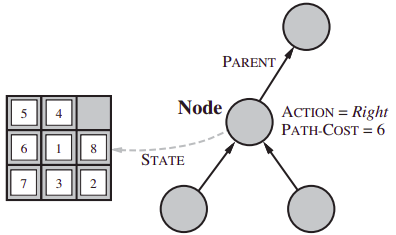
\includegraphics[
        width=0.5\linewidth,
        height=4cm,
        keepaspectratio,
    ]{images/artificial-intelligence/searching/search-node-sample.png}
    \caption*{Nodes are the data structures from which the search tree is constructed. Each has a parent, a state, and various bookkeeping fields. Arrows point from child to parent. \cite{ai/book/Artificial-Intelligence-A-Modern-Approach/Russell-Norvig}}
\end{figure}


\noindent
For each \textsc{Node} $n$ of the tree, we have a structure that contains four components:
\begin{enumerate}
    \item $n$.\textsc{State}: the state in the state space to which the node corresponds
    \hfill \cite{ai/book/Artificial-Intelligence-A-Modern-Approach/Russell-Norvig}

    \item $n$.\textsc{Parent}: the node in the search tree that generated this node
    \hfill \cite{ai/book/Artificial-Intelligence-A-Modern-Approach/Russell-Norvig}

    \item $n$.\textsc{Action}: the action that was applied to the parent to generate the node
    \hfill \cite{ai/book/Artificial-Intelligence-A-Modern-Approach/Russell-Norvig}

    \item $n$.\textsc{Path-Cost}: the cost, traditionally denoted by $g(n)$, of the path from the initial state to the node, as indicated by the parent pointers
    \hfill \cite{ai/book/Artificial-Intelligence-A-Modern-Approach/Russell-Norvig}
\end{enumerate}


\vspace{0.3cm}


\textbf{Note}:
\begin{enumerate}
    \item A node is a bookkeeping data structure used to represent the search tree.
    A state corresponds to a configuration of the world.
    Thus, nodes are on particular paths, as defined by \textsc{Parent} pointers, whereas states are not.
    Furthermore, two different nodes can contain the same world state if that state is generated via two different search paths.
    \hfill \cite{ai/book/Artificial-Intelligence-A-Modern-Approach/Russell-Norvig}

    \item The \textsc{Parent} pointers string the nodes together into a tree structure. These pointers also allow the solution path to be extracted when a goal node is found.
    \hfill \cite{ai/book/Artificial-Intelligence-A-Modern-Approach/Russell-Norvig}

    \item \textsc{Solution} function is used to return the sequence of actions obtained by following parent pointers back to the root.
    \hfill \cite{ai/book/Artificial-Intelligence-A-Modern-Approach/Russell-Norvig}
\end{enumerate}

\vspace{0.5cm}

\begin{lstlisting}[
    language=Python,
    caption=Problem Solving Agent - Search Node
]
class Node:
    def __init__(self, state, parent, action, path_cost):
        # the state in the state space to which the node corresponds
        self.state = state

        # the node in the search tree that generated this node
        self.parent = parent

        # the action that was applied to the parent to generate the node
        self.action = action

        """
            the cost, traditionally denoted by g(n), of the path
            from the initial state to the node, as indicated
            by the parent pointers
        """
        self.path_cost = path_cost

    def __lt__(self, __o):
        return self.path_cost < __o.path_cost

    def __str__(self):
        return (
            "<Node "
            + f"state: {self.state} "
            + f"parent: {self.parent} "
            + f"action: {self.action} "
            + f"path_cost: {self.path_cost} "
            + ">"
        )

    def __repr__(self) -> str:
        return str(self)
\end{lstlisting}



\begin{lstlisting}[
    language=Python,
    caption=Problem Solving Agent - solution
]
def solution(node: Node):
    path = []

    while node.parent is not None:
        path.insert(0, node.action)
        node = node.parent

    return path
\end{lstlisting}






\section{General Algorithms \& Implementations}

\subsection{Child-node}

\vspace{0.2cm}

\begin{algorithm}[H]
    \caption{The function \textsc{Child-Node} takes a parent node and an action and returns the resulting child node \cite{ai/book/Artificial-Intelligence-A-Modern-Approach/Russell-Norvig}}

    \SetKwFunction{FUNCTION}{\textsc{Child-Node}}
    \SetKwProg{Fn}{function}{ returns \normalfont{a \textsc{Node}}}{end}
    \Fn{\FUNCTION{problem}}{
        \Return a node with\\
            \hspace{1cm} \textsc{State} = $problem$.\textsc{Result}($parent$.\textsc{State}, $action$),\\
            \hspace{1cm} \textsc{Parent} = $parent$,\\
            \hspace{1cm} \textsc{Action} = $action$, \\
            \hspace{1cm} \textsc{Path-Cost} = $parent$.\textsc{Path-Cost} +
                $problem$.\textsc{Step-Cost}($parent$.\textsc{State}, $action$)
    }
\end{algorithm}


\begin{lstlisting}[
    language=Python,
    caption=Problem Solving Agents - child\_node
]
def child_node(problem: Problem, parent: Node, action):
    new_state = problem.result(parent.state, action)

    return Node(
        state=new_state,
        parent=parent,
        action=action,
        path_cost=(parent.path_cost
            + problem.step_cost(parent.state, action, new_state))
    )
\end{lstlisting}



\subsection{Tree Search}
\vspace{0.2cm}

\begin{algorithm}[H]
    \caption{An informal description of the general tree-search algorithm. \cite{ai/book/Artificial-Intelligence-A-Modern-Approach/Russell-Norvig}}

    \SetKwFunction{FUNCTION}{\textsc{Tree-Search}}
    \SetKwProg{Fn}{function}{ returns \normalfont{a solution, or failure}}{end}
    \Fn{\FUNCTION{problem}}{
        initialize the frontier using the initial state of problem\\
        \ \\
        \While{}{
            \If{the frontier is empty}{
                \Return failure
            }
            choose a leaf node and remove it from the frontier\\
            \If{the node contains a goal state}{
                \Return the corresponding solution
            }
            expand the chosen node, adding the resulting nodes to the frontier
        }
    }
\end{algorithm}


\begin{lstlisting}[
    language=Python,
    caption=Problem Solving Agents - tree\_search
]
def tree_search(problem: Problem):
    frontier = [Node(problem.initial_state, None, None, 0)]

    while True:
        if len(frontier) == 0:
            return None

        node: Node = frontier.pop()

        if problem.goal_test(node.state):
            return solution(node)

        for action in problem.actions(node.state):
            new_state = problem.result(node.state, action)
            path_cost = (node.path_cost
                + problem.step_cost(node.state, action, new_state))
            new_node = Node(new_state, node, action, path_cost)
            frontier.append(new_node)
\end{lstlisting}




\subsection{Graph search}
\vspace{0.2cm}

\begin{algorithm}[H]
    \caption{An informal description of the general graph-search algorithm. The parts of \textsc{Graph-Search} marked in bold italic are the additions needed to handle repeated states. \cite{ai/book/Artificial-Intelligence-A-Modern-Approach/Russell-Norvig}}

    \SetKwFunction{FUNCTION}{\textsc{Graph-Search}}
    \SetKwProg{Fn}{function}{ returns \normalfont{a solution, or failure}}{end}
    \Fn{\FUNCTION{problem}}{
        initialize the frontier using the initial state of problem \\
        \textbfit{initialize the explored set to be empty} \\
        \ \\
        \While{}{
            \If{the frontier is empty}{
                \Return failure
            }
            choose a leaf node and remove it from the frontier\\
            \If{the node contains a goal state}{
                \Return the corresponding solution
            }
            \textbfit{add the node to the explored set} \\
            \If{\bfseries chosen node not in the frontier or explored set}{
                expand the chosen node, adding the resulting nodes to the frontier
            }
        }
    }
\end{algorithm}

\begin{lstlisting}[
    language=Python,
    caption=Problem Solving Agents - graph\_search
]
def graph_search(problem: Problem):
    frontier = [Node(problem.initial_state, None, None, 0)]
    explored = set()

    while True:
        if len(frontier) == 0:
            return None

        node: Node = frontier.pop()

        if problem.goal_test(node.state):
            return solution(node)

        explored.add(node)

        for action in problem.actions(node.state):
            new_state = problem.result(node.state, action)
            path_cost = (node.path_cost
                + problem.step_cost(node.state, action, new_state))
            new_node = Node(new_state, node, action, path_cost)

            if new_node not in frontier and new_node not in explored:
                frontier.append(new_node)
\end{lstlisting}


\begin{enumerate}
    \item \textbf{explored set/ closed list}: remembers every expanded node
    \hfill \cite{ai/book/Artificial-Intelligence-A-Modern-Approach/Russell-Norvig}

    \item Newly generated nodes that match previously generated nodes - ones in the explored set or the frontier - can be discarded instead of being added to the frontier.
    \hfill \cite{ai/book/Artificial-Intelligence-A-Modern-Approach/Russell-Norvig}

    \item the search tree constructed by the \textsc{Graph-Search} algorithm contains \textbf{at most one copy} of each state, so we can think of it as growing a tree directly on the state-space graph.
    \hfill \cite{ai/book/Artificial-Intelligence-A-Modern-Approach/Russell-Norvig}

    \item The explored set can be implemented with a \textbf{hash table} to allow efficient checking for repeated states.
    \hfill \cite{ai/book/Artificial-Intelligence-A-Modern-Approach/Russell-Norvig}


\end{enumerate}



\section{Search Strategies/ Search Algorithms}

\subsection{Uninformed Search/ Blind Search}

\begin{enumerate}
    \item strategies have \textbf{no} additional information about states beyond that provided in the problem definition.
    \hfill \cite{ai/book/Artificial-Intelligence-A-Modern-Approach/Russell-Norvig}

    \item All they can do is generate successors and distinguish a goal state from a non-goal state. All search strategies are distinguished by the order in which nodes are expanded.
    \hfill \cite{ai/book/Artificial-Intelligence-A-Modern-Approach/Russell-Norvig}
\end{enumerate}


\vspace{0.3cm}
\textbf{SEE}:
\begin{enumerate}
    \item[] \fullref{AI: Algorithms/Breadth-first search (BFS)}
    \item[] \fullref{AI: Algorithms/Uniform-cost search (UCS)}
    \item[] \fullref{AI: Algorithms/Depth-first search (DFS)}
    \item[] \fullref{AI: Algorithms/Backtracking Search}
    \item[] \fullref{AI: Algorithms/Depth-limited search (DLS)}
    \item[] \fullref{AI: Algorithms/Iterative Deepening Search (IDS)}
    \item[] \fullref{AI: Algorithms/Iterative Lengthening Search (ILS)}
    \item[] \fullref{AI: Algorithms/Bidirectional search}
\end{enumerate}




\subsection{Informed Search/ Heuristic Search}

\begin{enumerate}
    \item Strategies that know whether one non-goal state is “\textit{more promising}” than another
    \hfill \cite{ai/book/Artificial-Intelligence-A-Modern-Approach/Russell-Norvig}

    \item uses problem-specific knowledge beyond the definition of the problem itself - can find solutions more efficiently than can an uninformed strategy.
    \hfill \cite{ai/book/Artificial-Intelligence-A-Modern-Approach/Russell-Norvig}


\end{enumerate}


\vspace{0.3cm}
\textbf{SEE}:
\begin{enumerate}
    \item[] \fullref{AI: Algorithms/Best-first search (BestFS)}
    \item[] \fullref{AI: Algorithms/Greedy best-first search (GBFS)}
    \item[] \fullref{AI: Algorithms/A* Search}
    \item[] \fullref{AI: Algorithms/Iterative-Deepening A* search}
    \item[] \fullref{AI: Algorithms/Recursive best-first search (RBFS)}
    \item[] \fullref{AI: Algorithms/Memory-Bounded A* (MA*) Search}
    \item[] \fullref{AI: Algorithms/Simplified Memory-Bounded A* (SMA*) Search}
\end{enumerate}


\subsection{Local Search}


\begin{table}[H]

\begin{minipage}[t]{0.55\linewidth}
\begin{figure}[H]
    \centering
    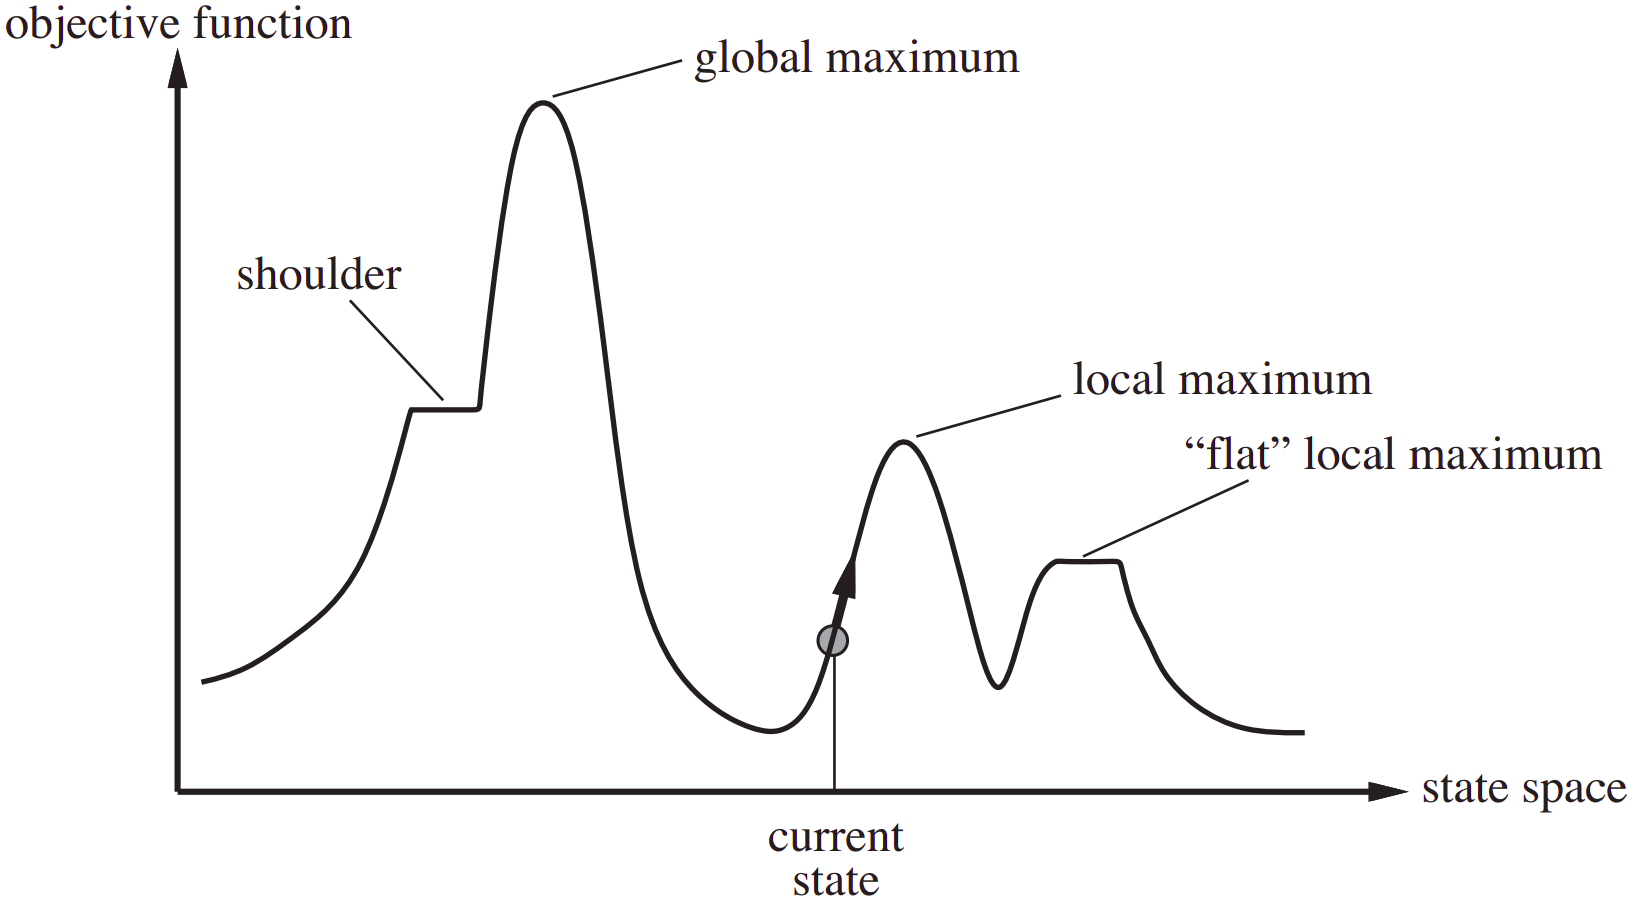
\includegraphics[
        width=\linewidth,
        height=6cm,
        keepaspectratio,
    ]{images/artificial-intelligence/searching/state-space-landscape--objective-function.png}
    \caption*{
        A one-dimensional \textbf{state-space landscape} in which elevation corresponds to the objective function. The aim is to find the global maximum.
        \cite{ai/book/Artificial-Intelligence-A-Modern-Approach/Russell-Norvig}
    }
\end{figure}
\end{minipage}
\hfill
\vrule
\hfill
\begin{minipage}[t]{0.40\linewidth}
\begin{figure}[H]
    \centering
    \includegraphics[
        width=\linewidth,
        height=5cm,
        keepaspectratio,
    ]{images/artificial-intelligence/searching/local-search-ridges.png}
    \caption*{
        The grid of states (dark circles) is superimposed on a ridge rising from left to right, creating a sequence of local maxima that are not directly connected to each other. From each local maximum, all the available actions point downhill.
        \cite{ai/book/Artificial-Intelligence-A-Modern-Approach/Russell-Norvig}
    }
\end{figure}
\end{minipage}


\end{table}




\begin{enumerate}
    \item[] {\fontsize{18}{18} \textbf{State-space landscape}}:

    \item A landscape has both “location” (defined by the state) and “elevation” (defined by the value of the heuristic cost function or objective function).
    \hfill \cite{ai/book/Artificial-Intelligence-A-Modern-Approach/Russell-Norvig}

    \item if elevation corresponds to cost, then the aim is to find the lowest valley (\textbf{global minimum})
    \hfill \cite{ai/book/Artificial-Intelligence-A-Modern-Approach/Russell-Norvig}

    \item if elevation corresponds to an objective function, then the aim is to find the highest peak (\textbf{global maximum})
    \hfill \cite{ai/book/Artificial-Intelligence-A-Modern-Approach/Russell-Norvig}

    \item These can convert from one to the other just by inserting a minus sign.
    \hfill \cite{ai/book/Artificial-Intelligence-A-Modern-Approach/Russell-Norvig}


    \item \textbf{Local maxima}: a local maximum is a peak that is higher than each of its neighboring states but lower than the global maximum.
    \hfill \cite{ai/book/Artificial-Intelligence-A-Modern-Approach/Russell-Norvig}

    \item \textbf{Ridges}:  Ridges result in a sequence of local maxima
    \hfill \cite{ai/book/Artificial-Intelligence-A-Modern-Approach/Russell-Norvig}

    \item \textbf{Plateaux}: a plateau is a flat area of the state-space landscape. It can be a \textbf{flat local maximum}, from which no uphill exit exists, or a \textbf{shoulder}, from which progress is possible.
    \hfill \cite{ai/book/Artificial-Intelligence-A-Modern-Approach/Russell-Norvig}







    \vspace{1cm}
    \item[] {\fontsize{18}{18} \textbf{Local Search}}:

    \item evaluates and modifies one or more current states rather than systematically exploring paths from an initial state.
    \hfill \cite{ai/book/Artificial-Intelligence-A-Modern-Approach/Russell-Norvig}

    \item These algorithms are suitable for problems in which all that matters is the solution state, not the path cost to reach it.
    these do not worry about paths at all.
    \hfill \cite{ai/book/Artificial-Intelligence-A-Modern-Approach/Russell-Norvig}

    \item The family of local search algorithms includes methods inspired by statistical physics (simulated annealing) and evolutionary biology (genetic algorithms).
    \hfill \cite{ai/book/Artificial-Intelligence-A-Modern-Approach/Russell-Norvig}

    \item Local search algorithms operate using a \textbf{single current node} (rather than multiple paths) and generally move only to neighbors of that node.
    Typically, the paths followed by the search are \textbf{not retained}.
    \hfill \cite{ai/book/Artificial-Intelligence-A-Modern-Approach/Russell-Norvig}

    \item local search algorithms are useful for solving \textbf{pure optimization problems}, in which the aim is to find the best state according to an \textbf{objective function}.
    \hfill \cite{ai/book/Artificial-Intelligence-A-Modern-Approach/Russell-Norvig}

    \item Many optimization problems do not fit the “standard” search models.
    \textbf{For example}: nature provides an objective function—reproductive fitness—that Darwinian evolution could be seen as attempting to optimize, but there is no “goal test” and no “path cost” for this problem.
    \hfill \cite{ai/book/Artificial-Intelligence-A-Modern-Approach/Russell-Norvig}

    \item  Local search algorithms explore this state-space landscape.
    \hfill \cite{ai/book/Artificial-Intelligence-A-Modern-Approach/Russell-Norvig}

    \item A complete local search algorithm always finds a goal if one exists.
    \hfill \cite{ai/book/Artificial-Intelligence-A-Modern-Approach/Russell-Norvig}

    \item An optimal algorithm always finds a global minimum/ maximum.
    \hfill \cite{ai/book/Artificial-Intelligence-A-Modern-Approach/Russell-Norvig}

    \item Local search algorithms typically use a \textbf{complete-state formulation}.
    \hfill  \cite{ai/book/Artificial-Intelligence-A-Modern-Approach/Russell-Norvig}

    \item \textbf{Advantages}:
    \begin{enumerate}
        \item they use very little memory—usually a constant amount
        \hfill \cite{ai/book/Artificial-Intelligence-A-Modern-Approach/Russell-Norvig}

        \item they can often find reasonable solutions in large or infinite (continuous) state spaces for which systematic algorithms are unsuitable
        \hfill \cite{ai/book/Artificial-Intelligence-A-Modern-Approach/Russell-Norvig}
    \end{enumerate}
\end{enumerate}





\subsection{Online Search}

\begin{enumerate}
    \item agent is faced with a state space that is initially unknown and must be explored.
    \hfill \cite{ai/book/Artificial-Intelligence-A-Modern-Approach/Russell-Norvig}



\end{enumerate}















\chapter{AI: Algorithms}\label{AI: Algorithms}

\begin{customArrayStretch}{1.3}
\begin{table}[H]
\centering
\begin{tabular}{r c p{12cm}}

$V$ & set & set of vertices (nodes) of the graph \\

$E$ & set  & set of edges (links) of the graph \\

$b$ & $\in \mathbb{R}$ & \textbf{branching factor} or maximum number of successors of any node \\

$d$ & $\in \mathbb{R}$ & \textbf{depth} of the \textbf{shallowest goal} node (i.e., the number of steps along the path from the root) \\

$m$ & $\in \mathbb{R}$ & maximum length of any path in the state space \\

$\varepsilon$ & $\in \mathbb{R}$ & minimum step cost (small positive constant) \\

$C$ & $\in \mathbb{R}$ & cost of the solution \\

$C^\ast$ & $\in \mathbb{R}$ & cost of the optimal solution \\

$\ell$ & $\in \mathbb{R}$ & predetermined depth limit \\

$G_n$ & node & goal node closest to $n$ \\

$M$ & $\in \mathbb{R}$ & memory bound \\

$N$ & $\in \mathbb{R}$ & total number of nodes generated \\





\hline





$g(n)$ & $\in \mathbb{R}$ & Path Cost (The \textbf{actual cost} from the \textbfit{start node} to the current node $n$) (Eg: UCS) \\

$h(n)$ & $\in \mathbb{R}$ & Heuristic Estimate (The \textbf{estimated cost} from node $n$ to the \textbfit{goal}) (Eg: GBFS, A*) \\

$f(n)$ & $\in \mathbb{R}$ & Evaluation Function (The \textbf{total estimated cost} of the \textbfit{cheapest solution} through $n$) (Eg: A*) \\

$h^\ast(n)$ & $\in \mathbb{R}$ & actual cost of getting from the root to the goal \\




\hline




$\Delta$ & $\in \mathbb{R}$ & \textbf{absolute error}: $\Delta \equiv h^\ast - h$  \\

$\epsilon$ \textbf{OR} $\Delta_r$ & 
$\in \mathbb{R}$ & 
\textbf{relative error}: $\epsilon \equiv \Delta_r \equiv (h^\ast - h)/h^\ast$ \\


$b^{\Delta_r}$ \textbf{OR} $b^\epsilon$ &
$\in \mathbb{R}$ & 
effective branching factor \\






\end{tabular}
\caption*{Notations}
\end{table}
\end{customArrayStretch}


\begin{enumerate}[itemsep=0.2cm]
    \item \textbf{heuristic function}
    \begin{enumerate}[itemsep=0.2cm]
        \item $h(n)$ = estimated cost of the cheapest path from the state at node $n$ to a goal state
        \hfill \cite{ai/book/Artificial-Intelligence-A-Modern-Approach/Russell-Norvig}

        \item Heuristic functions are the most common form in which additional knowledge of the problem is imparted to the search algorithm. 
        \hfill \cite{ai/book/Artificial-Intelligence-A-Modern-Approach/Russell-Norvig}
        
        \item if $n$ is a goal node, then $h(n)=0$
        \hfill \cite{ai/book/Artificial-Intelligence-A-Modern-Approach/Russell-Norvig}

        \item it depends only on the \textbfit{state} at that node.
        \hfill \cite{ai/book/Artificial-Intelligence-A-Modern-Approach/Russell-Norvig}

        \item the values of heuristic (eg: $h_{SLD}$) \textbf{may not} be computed from the problem description itself. Moreover, it takes a certain amount of experience to know that $h_{SLD}$ is correlated with actual road distances and is, therefore, a useful heuristic.
        \hfill \cite{ai/book/Artificial-Intelligence-A-Modern-Approach/Russell-Norvig}

        \item With a good heuristic function, however, the complexity can be reduced substantially. 
        The amount of the reduction depends on the particular problem and on the quality of the heuristic.
        \hfill \cite{ai/book/Artificial-Intelligence-A-Modern-Approach/Russell-Norvig}

        \item \textbf{admissible heuristic}: An admissible heuristic is one that \textbf{never overestimates} the cost to reach the goal. 
        Admissible heuristics are by nature optimistic because they think the cost of solving the problem is less than it actually is.
        \hfill \cite{ai/book/Artificial-Intelligence-A-Modern-Approach/Russell-Norvig}

        \item \textbf{consistency/ monotonicity}: A heuristic $h(n)$ is consistent if, for every node $n$ and every successor $n^\prime$ of $n$ generated by any action $a$, the estimated cost of reaching the goal from $n$ is no greater than the step cost of getting to $n^\prime$ plus the estimated cost of reaching the goal from $n$:
        \hfill \cite{ai/book/Artificial-Intelligence-A-Modern-Approach/Russell-Norvig}
        \\
        .\hfill $h(n) \leq c(n,\ a,\ n^\prime) + h(n^\prime)$
        \hfill \cite{ai/book/Artificial-Intelligence-A-Modern-Approach/Russell-Norvig}
        \\
        \textbf{every} consistent heuristic is also admissible
        \hfill \cite{ai/book/Artificial-Intelligence-A-Modern-Approach/Russell-Norvig}

        \item Consistency is a stricter requirement than admissibility, but one has to work quite hard to concoct heuristics that are admissible but not consistent.
        \hfill \cite{ai/book/Artificial-Intelligence-A-Modern-Approach/Russell-Norvig}

        \item if $h(n)$ is consistent, then the values of $f(n)$ along any path are non-decreasing
        \hfill \cite{ai/book/Artificial-Intelligence-A-Modern-Approach/Russell-Norvig}

        \item For almost all heuristics in practical use, the absolute error is at least proportional to the path cost $h^\ast$, so $\epsilon$ is constant or growing and the time complexity is exponential in $d$.
        \hfill \cite{ai/book/Artificial-Intelligence-A-Modern-Approach/Russell-Norvig}

        \item When the state space has many goal states - particularly \textbf{near-optimal goal} states - the search process can be led astray from the optimal path and there is an extra cost proportional to the number of goals whose cost is within a factor  of the optimal cost.
        \hfill \cite{ai/book/Artificial-Intelligence-A-Modern-Approach/Russell-Norvig}

        \item experimental measurements of b$^\ast$ on a small set of problems can provide a good guide to the heuristic’s overall usefulness. 
        A well-designed heuristic would have a value of b$^\ast$ close to $1$, allowing fairly large problems to be solved at reasonable computational cost.
        \hfill \cite{ai/book/Artificial-Intelligence-A-Modern-Approach/Russell-Norvig}

        \item \textbf{Dominating heuristic}: if for any node $n$, $h_2(n) \geq h_1(n)$, $h_2$ \textbf{dominates} $h_1$.
        Domination translates directly into efficiency: algorithm using $h_2$ will \textbf{never} expand more nodes than same algorithm using $h_1$ 
        (except possibly for some nodes with $f(n) = C^\ast$).
        \hfill \cite{ai/book/Artificial-Intelligence-A-Modern-Approach/Russell-Norvig}
        \\
        For A$^\ast$ search, every node with $f(n) < C^\ast$ will surely be expanded.
        This is the same as saying that every node with $h(n) < C^\ast - g(n)$ will surely be expanded.
        \hfill \cite{ai/book/Artificial-Intelligence-A-Modern-Approach/Russell-Norvig}
    \end{enumerate}

    \item \textbf{evaluation function}:
    \begin{enumerate}[itemsep=0.2cm]
        \item The evaluation function $f$ is construed/ interpreted as a cost estimate, so the node with the lowest evaluation is expanded first.
        \hfill \cite{ai/book/Artificial-Intelligence-A-Modern-Approach/Russell-Norvig}
        
        \item The choice of $f$ determines the search strategy.
        \hfill \cite{ai/book/Artificial-Intelligence-A-Modern-Approach/Russell-Norvig}

        \item $f(n) = g(n)$ or $h(n)$ or $g(n)+h(n)$ or something else depending on the algorithm

        \item The fact that $f$-costs are \textit{non-decreasing} along any path also means that we can draw \textbf{contours} in the state space, just like the contours in a topographic map. 
        With more accurate heuristics, the bands will stretch toward the goal state and become more narrowly focused around the optimal path.
        \hfill \cite{ai/book/Artificial-Intelligence-A-Modern-Approach/Russell-Norvig}

        \item There can be exponentially many states with $f(n) < C^\ast$ even if the absolute error is bounded by a constant.
        \hfill \cite{ai/book/Artificial-Intelligence-A-Modern-Approach/Russell-Norvig}

        
    \end{enumerate}

    \item memory limitations can make a problem intractable from the point of view of computation time
    \hfill \cite{ai/book/Artificial-Intelligence-A-Modern-Approach/Russell-Norvig}

    \item The effective branching factor can vary across problem instances, but usually it is fairly constant for sufficiently hard problems.
    \hfill \cite{ai/book/Artificial-Intelligence-A-Modern-Approach/Russell-Norvig}
\end{enumerate}





\section{Breadth-first search (BFS) \cite{ai/book/Artificial-Intelligence-A-Modern-Approach/Russell-Norvig}}
\label{AI: Algorithms/Breadth-first search (BFS)}


\begin{figure}[H]
    \centering
    \includegraphics[
        width=\linewidth,
        height=4cm,
        keepaspectratio,
    ]{images/algorithms/Breadth-first-search-BT.png}
    \caption*{
        Breadth-first search on a simple binary tree. At each stage, the node to be expanded next is indicated by a marker.
        \cite{ai/book/Artificial-Intelligence-A-Modern-Approach/Russell-Norvig}
    }
\end{figure}


\begin{enumerate}[itemsep=0.2cm]
    \item Breadth-first search is a simple strategy in which the root node is expanded first, then all the successors of the root node are expanded next, then their successors, and so on. 
    \hfill \cite{ai/book/Artificial-Intelligence-A-Modern-Approach/Russell-Norvig}

    \item In general, all the nodes are expanded at a given depth in the search tree before any nodes at the next level are expanded.
    \hfill \cite{ai/book/Artificial-Intelligence-A-Modern-Approach/Russell-Norvig}

    \item Breadth-first search is an instance of the general graph-search algorithm in which the \textit{shallowest unexpanded node} is chosen for expansion.
    \hfill \cite{ai/book/Artificial-Intelligence-A-Modern-Approach/Russell-Norvig}

    \item new nodes (which are always deeper than their parents) go to the back of the queue, and old nodes, which are shallower than the new nodes, get expanded first. 
    \hfill \cite{ai/book/Artificial-Intelligence-A-Modern-Approach/Russell-Norvig}

    \item There is one slight tweak on the general graph-search algorithm, which is that the goal test is applied to each node when it is generated rather than when it is selected for expansion.
    \hfill \cite{ai/book/Artificial-Intelligence-A-Modern-Approach/Russell-Norvig}
    \\
    If the algorithm were to apply the goal test to nodes when selected for expansion, rather than when generated, the whole layer of nodes at depth d would be expanded before the goal was detected and the time complexity would be $\mathcal{O}(b\ ^{d+1})$.
    \hfill \cite{ai/book/Artificial-Intelligence-A-Modern-Approach/Russell-Norvig}

    \item the algorithm, following the general template for graph search, discards any new path to a state already in the frontier or explored set; it is easy to see that any such path must be at least as deep as the one already found. 
    \hfill \cite{ai/book/Artificial-Intelligence-A-Modern-Approach/Russell-Norvig}

    \item breadth-first search \textbf{always} has the \textit{shallowest path} to every node on the frontier. 
    As soon as a goal node is generated, we know it is the shallowest goal node because all shallower nodes must have been generated already and failed the goal test. 
    \hfill \cite{ai/book/Artificial-Intelligence-A-Modern-Approach/Russell-Norvig}

    \item \textbf{performance}:
    \begin{enumerate}[itemsep=0.2cm]
        \item \textbf{complete}: if the shallowest goal node is at some finite depth $d$, breadth-first search will eventually find it after generating all shallower nodes (provided the branching factor $b$ is finite). 
        \hfill \cite{ai/book/Artificial-Intelligence-A-Modern-Approach/Russell-Norvig}

        \item  the shallowest goal node is \textbf{not necessarily} the \textit{optimal} one. 
        breadth-first search is optimal if the path cost is a non-decreasing function of the depth of the node.
        The most common such scenario is that all actions have the same cost.
        the algorithm is optimal if step costs are all identical.
        \hfill \cite{ai/book/Artificial-Intelligence-A-Modern-Approach/Russell-Norvig}

        \item \textbf{Space Complexity}:
        \begin{enumerate}[itemsep=0.1cm]
            \item explored set: $\mathcal{O}(b\ ^{d-1})$
            \hfill \cite{ai/book/Artificial-Intelligence-A-Modern-Approach/Russell-Norvig}

            \item frontier: $\mathcal{O}(b\ ^{d})$
            \hfill \cite{ai/book/Artificial-Intelligence-A-Modern-Approach/Russell-Norvig}

            \item overall: $\mathcal{O}(b\ ^{d})$
            \hfill \cite{ai/book/Artificial-Intelligence-A-Modern-Approach/Russell-Norvig}
        \end{enumerate}

        \item \textbf{Time Complexity}: 
        $\mathcal{O}(b\ ^{d})$
        \hfill \cite{ai/book/Artificial-Intelligence-A-Modern-Approach/Russell-Norvig}

    \end{enumerate}

    \item \textbf{Disadvantages}:
    \begin{enumerate}[itemsep=0.1cm]
        \item the memory requirements are a bigger problem for breadth-first search than is the execution time.
        \hfill \cite{ai/book/Artificial-Intelligence-A-Modern-Approach/Russell-Norvig}

        
    \end{enumerate}

\end{enumerate}


\subsection*{Implementation}

\begin{enumerate}
    \item \textbf{frontier}: FIFO queue
\end{enumerate}


\vspace{0.5cm}


\begin{algorithm}[H]
    \caption{Breadth-first search on a graph. \cite{ai/book/Artificial-Intelligence-A-Modern-Approach/Russell-Norvig}}

    \SetKwFunction{FUNCTION}{\textsc{Breadth-First-Search}}
    \SetKwProg{Fn}{function}{ returns \normalfont{a solution, or failure}}{end}
    \Fn{\FUNCTION{problem}}{
        $node \ \gets$ a node with \textsc{State} = $problem$.\textsc{Initial-State}, \textsc{Path-Cost} = $0$ \\
        \ \\
        \If{$problem$.\textsc{Goal-Test}($node$.\textsc{State})}{
            \Return \textsc{Solution}($node$)
        }
        \ \\
        $frontier \ \gets$ a FIFO queue with node as the only element \\
        $explored \ \gets$ an empty set \\
        \ \\
        \While{}{
            \If{\textsc{Empty?}($frontier$)}{
                \Return failure
            }
            \ \\
            \Comment{chooses the shallowest node in $frontier$}
            $node \ \gets$ \textsc{Pop}($frontier$) \\ 
            add $node$.\textsc{State} to $explored$ \\
            \ \\
            \ForEach{$action$ \textbf{in} $problem$.\textsc{Actions}($node$.\textsc{State})}{
                $child \gets$ \textsc{Child-Node}($problem,\ node,\ action$) \\
                \If{$child$.\textsc{State} is \textbf{not in} $explored$ or $frontier$}{
                    \If{$problem$.\textsc{Goal-Test}($child$.\textsc{State})}{
                        \Return \textsc{Solution}($child$)
                    }
                    $frontier \gets$ \textsc{Insert}($child,\ frontier$)
                }
            }
        }
    }
\end{algorithm}


\begin{lstlisting}[
    language=Python,
    caption=Problem Solving Agent - Breadth-first search on a graph
]
from queue import Queue

def breadth_first_search(problem: Problem):
    node = Node(problem.initial_state, None, None, 0)

    if problem.goal_test(node.state):
        return solution(node)
    
    frontier = Queue()
    explored = set()

    frontier.put(node)

    while True:
        if frontier.empty():
            return None
        
        node = frontier.get()
        explored.add(node)

        for action in problem.actions(node.state):
            child = child_node(problem, node, action)
            
            if (not any([n.state == child.state for n in frontier.queue]) and 
                not any([n.state == child.state for n in explored])):
                if problem.goal_test(child.state):            
                    return solution(child)

                frontier.put(child)
\end{lstlisting}












\section{Uniform-cost search (UCS) \cite{ai/book/Artificial-Intelligence-A-Modern-Approach/Russell-Norvig}}
\label{AI: Algorithms/Uniform-cost search (UCS)}


\begin{enumerate}[itemsep=0.2cm]
    \item Instead of expanding the shallowest node (as in BFS), uniform-cost search expands the node $n$ with the \textbfit{lowest path cost} $g(n)$.
    \hfill \cite{ai/book/Artificial-Intelligence-A-Modern-Approach/Russell-Norvig}

    \item \textbf{Performance}:
    \begin{enumerate}[itemsep=0.2cm]
        \item uniform-cost search is \textbf{optimal} in general. 
        uniform-cost search expands nodes in order of their optimal path cost.
        \hfill \cite{ai/book/Artificial-Intelligence-A-Modern-Approach/Russell-Norvig}

        \item \textbf{Completeness is guaranteed} provided the cost of every step exceeds some small positive constant $\varepsilon$ and $b$ is finite
        \hfill \cite{ai/book/Artificial-Intelligence-A-Modern-Approach/Russell-Norvig}

        \item \textbf{Space Complexity}:
        \begin{enumerate}[itemsep=0.2cm]
            \item worst: $\mathcal{O}(b^{1 + \dfloor{C^\ast / \varepsilon}})$
            \hfill (can be much greater than $b^d$)
            \hfill \cite{ai/book/Artificial-Intelligence-A-Modern-Approach/Russell-Norvig}

            \item When all step costs are equal: $\mathcal{O}(b^{\ d+1})$
            \hfill \cite{ai/book/Artificial-Intelligence-A-Modern-Approach/Russell-Norvig}
        \end{enumerate}

        \item \textbf{Time Complexity}:
        \begin{enumerate}[itemsep=0.2cm]
            \item worst: $\mathcal{O}(b^{1 + \dfloor{C^\ast / \varepsilon}})$
            \hfill (can be much greater than $b^d$)
            \hfill \cite{ai/book/Artificial-Intelligence-A-Modern-Approach/Russell-Norvig}

            \item When all step costs are equal: $\mathcal{O}(b^{\ d+1})$
            \hfill \cite{ai/book/Artificial-Intelligence-A-Modern-Approach/Russell-Norvig}
        \end{enumerate}
    \end{enumerate}

    \item \textbf{Disadvantages}:
    \begin{enumerate}[itemsep=0.2cm]
        \item it will get stuck in an \textbf{infinite loop} if there is a path with an infinite sequence of \textit{zero-cost actions} - for example, a sequence of $NoOp$ actions.
        \hfill \cite{ai/book/Artificial-Intelligence-A-Modern-Approach/Russell-Norvig}

        \item  it suffers from the same difficulties with realvalued costs
        \hfill \cite{ai/book/Artificial-Intelligence-A-Modern-Approach/Russell-Norvig}
    \end{enumerate}

    \item When all step costs are the same, uniform-cost search is similar to breadth-first search, except that the latter stops as soon as it generates a goal, whereas uniform-cost search examines all the nodes at the goal’s depth to see if one has a lower cost; thus uniform-cost search does strictly more work by expanding nodes at depth $d$ unnecessarily.
    \hfill \cite{ai/book/Artificial-Intelligence-A-Modern-Approach/Russell-Norvig}
\end{enumerate}




\subsection*{Implementation}

\begin{enumerate}
    \item  This is done by storing the frontier as a \textbf{priority queue} ordered by $g(n)$. 
    \hfill \cite{ai/book/Artificial-Intelligence-A-Modern-Approach/Russell-Norvig}

    \item In addition to the ordering of the queue by path cost, there are two other significant differences from breadth-first search.
    \hfill \cite{ai/book/Artificial-Intelligence-A-Modern-Approach/Russell-Norvig}
    \begin{enumerate}
        \item  goal test is applied to a node when it is \textit{selected for expansion} rather than when it is first generated.
        The reason is that the first goal node that is \textit{generated} may be on a suboptimal path.
        \hfill \cite{ai/book/Artificial-Intelligence-A-Modern-Approach/Russell-Norvig}

        \item a test is added in case a better path is found to a node currently on the frontier.
        \hfill \cite{ai/book/Artificial-Intelligence-A-Modern-Approach/Russell-Norvig}
    \end{enumerate}

\end{enumerate}

\vspace{0.5cm}


\begin{algorithm}[H]
    \caption{\textsc{Uniform-Cost} search on a graph. \cite{ai/book/Artificial-Intelligence-A-Modern-Approach/Russell-Norvig}}

    \SetKwFunction{FUNCTION}{\textsc{Uniform-Cost-Search}}
    \SetKwProg{Fn}{function}{ returns \normalfont{a solution, or failure}}{end}
    \Fn{\FUNCTION{problem}}{
        $node \ \gets$ a node with \textsc{State} = $problem$.\textsc{Initial-State}, \textsc{Path-Cost} = $0$ \\
        $frontier \ \gets$ a \textbfit{priority queue} ordered by \textsc{Path-Cost}, with $node$ as the only element \\
        $explored \ \gets$ an empty set \\
        \ \\
        \While{}{
            \lIf{\textsc{Empty?}($frontier$)}{
                \Return failure
            }
            \Comment{chooses the lowest-cost node in $frontier$}
            $node \ \gets$ \textsc{Pop}($frontier$) \\ 
            \lIf{$problem$.\textsc{Goal-Test}($node$.\textsc{State})}{
                \Return \textsc{Solution}($node$)
            }
            add $node$.\textsc{State} to $explored$ \\
            \ \\
            \ForEach{$action$ \textbf{in} $problem$.\textsc{Actions}($node$.\textsc{State})}{
                $child \gets$ \textsc{Child-Node}($problem,\ node,\ action$) \\
                \If{\normalfont $child$.\textsc{State} is not in $explored$ or $frontier$}{
                    $frontier \gets$ \textsc{Insert}($child,\ frontier$)
                }
                \ElseIf{\normalfont $child$.\textsc{State} is in $frontier$ with higher \textsc{Path-Cost}}{
                    replace that $frontier$ node with $child$
                }
            }
        }
    }
\end{algorithm}


\begin{lstlisting}[
    language=Python,
    caption=Problem Solving Agent - Uniform cost search on a graph
]
import heapq

def uniform_cost_search(problem: Problem):
    node = Node(problem.initial_state, None, None, 0)

    if problem.goal_test(node.state):
        return solution(node)
    
    frontier = [(node.path_cost, node)]
    explored = set()

    heapq.heapify(frontier)

    while True:
        if len(frontier) == 0:
            return None
        
        path_cost, node = frontier.pop(0)

        if problem.goal_test(node.state):
            return solution(node)

        explored.add(node)
        for action in problem.actions(node.state):
            child = child_node(problem, node, action)

            if (not any([n.state == child.state for (path_cost, n) in frontier])
                and not any([n.state == child.state for n in explored])):
                frontier.append((child.path_cost, child))
                heapq.heapify(frontier)
            else:
                for idx, (path_cost, n) in enumerate(frontier):
                    if n.state == child.state and path_cost > child.path_cost:
                        frontier[idx] = (child.path_cost, child)
                        heapq.heapify(frontier)
\end{lstlisting}






\section{Depth-first search (DFS) \cite{ai/book/Artificial-Intelligence-A-Modern-Approach/Russell-Norvig}}


\begin{figure}[H]
\centering
\includegraphics[
    width=\linewidth,
    height=7cm,
    keepaspectratio,
]{images/algorithms/Depth-first-search-illustration.png}
\caption*{
    Depth-first search on a binary tree. The unexplored region is shown in light gray. Explored nodes with no descendants in the frontier are removed from memory. Nodes at depth $3$ have no successors and $M$ is the only goal node. 
    \cite{ai/book/Artificial-Intelligence-A-Modern-Approach/Russell-Norvig}
}
\end{figure}


\begin{enumerate}[itemsep=0.2cm]
    \item Depth-first search always expands the \textbf{deepest node} in the current frontier of the search tree.
    \hfill \cite{ai/book/Artificial-Intelligence-A-Modern-Approach/Russell-Norvig}

    \item The search proceeds immediately to the deepest level of the search tree, where the nodes have no successors. As those nodes are expanded, they are dropped from the frontier, so then the search “backs up” to the next deepest node that still has unexplored successors.
    \hfill \cite{ai/book/Artificial-Intelligence-A-Modern-Approach/Russell-Norvig}

    \item \textbf{Performance}:
    \begin{enumerate}[itemsep=0.2cm]
        \item \textbf{graph-search version}:
        \begin{enumerate}[itemsep=0.2cm]
            \item \textbf{complete} in finite state spaces because it will eventually expand every node
            \hfill \cite{ai/book/Artificial-Intelligence-A-Modern-Approach/Russell-Norvig}

            \item \textbf{not optimal}
            \hfill \cite{ai/book/Artificial-Intelligence-A-Modern-Approach/Russell-Norvig}

            \item \textbf{time complexity}: $\mathcal{O}(b^d)$
            \hfill \cite{ai/book/Artificial-Intelligence-A-Modern-Approach/Russell-Norvig}

            \item \textbf{space complexity}: $\mathcal{O}(b^d)$
            \hfill \cite{ai/book/Artificial-Intelligence-A-Modern-Approach/Russell-Norvig}
        \end{enumerate}

        \item \textbf{tree-search version}:
        \begin{enumerate}[itemsep=0.2cm]
            \item \textbf{not complete}, as it can fall in \textit{infinite loop}
            \hfill \cite{ai/book/Artificial-Intelligence-A-Modern-Approach/Russell-Norvig}

            \item \textbf{not optimal}
            \hfill \cite{ai/book/Artificial-Intelligence-A-Modern-Approach/Russell-Norvig}

            \item \textbf{time complexity}: $\mathcal{O}(b^m)$
            \hfill \cite{ai/book/Artificial-Intelligence-A-Modern-Approach/Russell-Norvig}

            \item \textbf{space complexity}: $\mathcal{O}(b\ m)$
            \hfill \cite{ai/book/Artificial-Intelligence-A-Modern-Approach/Russell-Norvig}
        \end{enumerate}
    \end{enumerate}
\end{enumerate}


\subsection{Implementation}

\begin{enumerate}[itemsep=0.2cm]
    \item The depth-first search algorithm is an instance of the graph-search algorithm that uses a LIFO queue.
    \hfill \cite{ai/book/Artificial-Intelligence-A-Modern-Approach/Russell-Norvig}

    \item  it is common to implement depth-first search with a recursive function that calls itself  on each of its children in turn. 
    \hfill \cite{ai/book/Artificial-Intelligence-A-Modern-Approach/Russell-Norvig}
\end{enumerate}

\begin{lstlisting}[
    language=Python,
    caption=Problem Solving Agent - Depth first search on a graph
]
from queue import LifoQueue

def depth_first_search(problem: Problem):
    node = Node(problem.initial_state, None, None, 0)

    if problem.goal_test(node.state):
        return solution(node)
    
    frontier = LifoQueue()
    explored = set()

    frontier.put(node)

    while True:
        if frontier.empty():
            return None
        
        node = frontier.get()
        explored.add(node)

        for action in problem.actions(node.state):
            child = child_node(problem, node, action)

            if (not any([n.state == child.state for n in frontier.queue]) and 
                not any([n.state == child.state for n in explored])):
                if problem.goal_test(child.state):
                    return solution(child)

                frontier.put(child)
\end{lstlisting}















\section{Backtracking Search \cite{ai/book/Artificial-Intelligence-A-Modern-Approach/Russell-Norvig}}
\label{AI: Algorithms/Backtracking Search}


\begin{enumerate}
    \item A variant of depth-first search that uses still less memory.
    \hfill \cite{ai/book/Artificial-Intelligence-A-Modern-Approach/Russell-Norvig}

    \item \textbf{only one successor} is generated at a time rather than all successors; each partially expanded node remembers which successor to generate next.
    \hfill \cite{ai/book/Artificial-Intelligence-A-Modern-Approach/Russell-Norvig}

    \item \textbf{Performance}:
    \begin{enumerate}
        \item \textbf{Space Complexity}: $\mathcal{O}(m)$
        \hfill \cite{ai/book/Artificial-Intelligence-A-Modern-Approach/Russell-Norvig}
    \end{enumerate}

    \item \textbf{Advantages}:
    \begin{enumerate}
        \item  Backtracking search facilitates memory-saving (and time-saving) trick: the idea of generating a successor by \textbf{modifying} the current state description directly rather than copying it first.
        For this to work, we must be able to \textbf{undo} each modification when we go back to generate the next successor.
        \hfill \cite{ai/book/Artificial-Intelligence-A-Modern-Approach/Russell-Norvig}

        \item For problems with large state descriptions, such as robotic assembly, these techniques are critical to success.
        \hfill \cite{ai/book/Artificial-Intelligence-A-Modern-Approach/Russell-Norvig}
    \end{enumerate}
\end{enumerate}



\begin{lstlisting}[
    language=Python,
    caption=Problem Solving Agent - Backtracking using recursion \cite{common/online/chatgpt}
]
def backtrack(node: Node, explored: set):
    if problem.goal_test(node.state):
        return solution(node)

    explored.add(node)

    for action in problem.actions(node.state):
        child = child_node(problem, node, action)
        if not any([child.state == n.state for n in explored]):
            result = backtrack(child, explored)
            if result is not None:
                return result

    # Optional: allow revisiting for other paths (depends on problem)
    explored.remove(node)
    return None

def backtracking_search(problem: Problem):
    root = Node(problem.initial_state, None, None, 0)
    return backtrack(root, set())
\end{lstlisting}















\section{Depth-limited search \cite{ai/book/Artificial-Intelligence-A-Modern-Approach/Russell-Norvig}}

\begin{enumerate}[itemsep=0.2cm]
    \item The embarrassing failure of depth-first search in infinite state spaces can be alleviated by supplying depth-first search with a predetermined depth limit $\ell$. That is, nodes at depth  $\ell$ are treated as if they have no successors. 
    \hfill \cite{ai/book/Artificial-Intelligence-A-Modern-Approach/Russell-Norvig}

    \item \textbf{Performance}:
    \begin{enumerate}
        \item \textbf{Completeness}: NO \textbf{if} $\ell < d$ \textbf{else} YES
        \hfill \cite{ai/book/Artificial-Intelligence-A-Modern-Approach/Russell-Norvig}

        \item \textbf{Optimal}: NO \textbf{if} $\ell > d$ \textbf{else} YES
        \hfill \cite{ai/book/Artificial-Intelligence-A-Modern-Approach/Russell-Norvig}

        \item \textbf{time complexity}: $\mathcal{O}(b^\ell)$
        \hfill \cite{ai/book/Artificial-Intelligence-A-Modern-Approach/Russell-Norvig}

        \item \textbf{space complexity}: $\mathcal{O}(b\ell)$
        \hfill \cite{ai/book/Artificial-Intelligence-A-Modern-Approach/Russell-Norvig}
    \end{enumerate}

    \item Depth-first search can be viewed as a special case of depth-limited search with $\ell = \infty$.
    \hfill \cite{ai/book/Artificial-Intelligence-A-Modern-Approach/Russell-Norvig}

    \item diameter of the state space can be a better limit for efficiency
    \hfill \cite{ai/book/Artificial-Intelligence-A-Modern-Approach/Russell-Norvig}

    
\end{enumerate}


\vspace{0.5cm}

\begin{algorithm}[H]
    \caption{A recursive implementation of depth-limited tree search. \cite{ai/book/Artificial-Intelligence-A-Modern-Approach/Russell-Norvig}}


    \SetKwFunction{FUNCTION}{\textsc{Depth-Limited-Search}}
    \SetKwProg{Fn}{function}{ returns \normalfont{a solution, or failure/cutoff}}{end}
    \Fn{\FUNCTION{problem, limit}}{
        \Return \textsc{Recursive-DLS}( \\
            \hspace{0.5cm}  \textsc{Make-Node}($problem$.\textsc{Initial-State}), \\
            \hspace{0.5cm}  $problem$, \\
            \hspace{0.5cm}  $limit$, \\
        )
    }
    
    \ \\
    
    \SetKwFunction{FUNCTION}{\textsc{Recursive-DLS}}
    \SetKwProg{Fn}{function}{ returns \normalfont{a solution, or failure/cutoff}}{end}
    \Fn{\FUNCTION{node, problem, limit}}{
        \If{\normalfont $problem$.\textsc{Goal-Test}($node$.\textsc{State})}{
            \Return \textsc{Solution}($node$) 
        }
        \ElseIf{limit = 0}{
            \Return $cutoff$
        }
        \Else{
            $cutoff\_occurred? \ \gets$ false\\
            \ \\
            \ForEach{\normalfont $action$ \textbf{in} $problem$.\textsc{Actions}($node$.\textsc{State})}{
                $child \gets$ \textsc{Child-Node}($problem,\ node,\ action$)\\
                $result \gets$ \textsc{Recursive-DLS}($child,\ problem,\ limit-1$)\\
                \If{result = cutoff}{
                    $cutoff\_occurred? \ \gets$ true
                }
                \ElseIf{result $\neq$ failure}{
                    \Return $result$
                }
            }
            \ \\
            \If{$cutoff\_occurred?$}{
                \Return $cutoff$
            }
            \Else{
                \Return $failure$
            }
        }
    }
\end{algorithm}


\begin{lstlisting}[
    language=Python,
    caption=Problem Solving Agent - Depth limited search (recursive)
]
CUTOFF = "CUT-OFF"

def depth_limited_search(problem: Problem, limit: int):
    return recursive_dls(
        Node(problem.initial_state, None, None, 0),
        problem,
        limit,
    )

def recursive_dls(node: Node, problem: Problem, limit: int):
    if problem.goal_test(node.state):
        return solution(node)
    
    elif limit == 0:
        return CUTOFF
    
    else:
        cutoff_occurred = False
        for action in problem.actions(node.state):
            child = child_node(problem, node, action)
            result = recursive_dls(child, problem, limit-1)
            if result == CUTOFF:
                cutoff_occurred = True
            elif result is not None:
                return result
        if cutoff_occurred:
            return CUTOFF
        else:
            return
\end{lstlisting}


\vspace{0.5cm}

\begin{enumerate}[itemsep=0.2cm]
    \item $failure$ value indicates no solution
    \hfill \cite{ai/book/Artificial-Intelligence-A-Modern-Approach/Russell-Norvig}

    \item $cutoff$ value indicates no solution within the depth limit
    \hfill \cite{ai/book/Artificial-Intelligence-A-Modern-Approach/Russell-Norvig}
\end{enumerate}








\section{Iterative Deepening Search (IDS) \cite{ai/book/Artificial-Intelligence-A-Modern-Approach/Russell-Norvig}}
\label{AI: Algorithms/Iterative Deepening Search (IDS)}


\begin{figure}[h!]
    \centering
    \includegraphics[
        width=\linewidth,
        height=14cm,
        keepaspectratio,
    ]{images/algorithms/iterative-deepening-search-BT.png}
    \caption*{Four iterations of iterative deepening search on a binary tree \cite{ai/book/Artificial-Intelligence-A-Modern-Approach/Russell-Norvig}}
\end{figure}


\begin{enumerate}
    \item \textbf{Iterative deepening search} (or \textbf{iterative deepening depth-first search}) is a general strategy, often used in combination with depth-first tree search, that finds the best depth limit.
    \hfill \cite{ai/book/Artificial-Intelligence-A-Modern-Approach/Russell-Norvig}

    \item It gradually increases the depth limit $\ell \in \dCurlyBrac{0,1,2,\cdots,\infty}$ till a goal is found, which occurs when $\ell = d$ ($d$ is unknown in reality)
    \hfill \cite{ai/book/Artificial-Intelligence-A-Modern-Approach/Russell-Norvig}

    \item Iterative deepening combines the benefits of depth-first and breadth-first search.
    \hfill \cite{ai/book/Artificial-Intelligence-A-Modern-Approach/Russell-Norvig}
    \begin{enumerate}
        \item Like depth-first search, its memory requirements are modest: $\mathcal{O}(b d)$ to be precise. 
        \hfill \cite{ai/book/Artificial-Intelligence-A-Modern-Approach/Russell-Norvig}

        \item Like breadth-first search, it is complete when the branching factor is finite and optimal when the path cost is a non-decreasing function of the depth of the node.
        \hfill \cite{ai/book/Artificial-Intelligence-A-Modern-Approach/Russell-Norvig}
    \end{enumerate}

    \item total number of nodes generated in the worst case is
    \\
    $N(\text{IDS})=(d)b + (d - 1)b^2 + \cdots + (1)b^d$
    \hfill \cite{ai/book/Artificial-Intelligence-A-Modern-Approach/Russell-Norvig}

    \item you can use a hybrid approach that runs breadth-first search until almost all the available memory is consumed, and then runs iterative deepening from all the nodes in the frontier.
    \hfill \cite{ai/book/Artificial-Intelligence-A-Modern-Approach/Russell-Norvig}

    \item iterative deepening is the \textit{preferred uninformed search} method when the search space is large and the depth of the solution is not known.
    \hfill \cite{ai/book/Artificial-Intelligence-A-Modern-Approach/Russell-Norvig}

    \item \textbf{Performance}:
    \begin{enumerate}
        \item \textbf{completeness}: YES \textbf{if} $b$ is finite \textbf{else} NO
        \hfill \cite{ai/book/Artificial-Intelligence-A-Modern-Approach/Russell-Norvig}

        \item \textbf{optimal}: YES \textbf{if} path cost is a non-deceasing function of depth of the node \textbf{else} NO
        \hfill \cite{ai/book/Artificial-Intelligence-A-Modern-Approach/Russell-Norvig}
        
        \item \textbf{space complexity}: $\mathcal{O}(b d)$
        \hfill \cite{ai/book/Artificial-Intelligence-A-Modern-Approach/Russell-Norvig}

        \item \textbf{time complexity}: $\mathcal{O}(b^d)$
        \hfill \cite{ai/book/Artificial-Intelligence-A-Modern-Approach/Russell-Norvig}
    \end{enumerate}
\end{enumerate}

\vspace{0.5cm}

\begin{algorithm}[H]
    \caption{The iterative deepening search algorithm, which repeatedly applies depth-limited search with increasing limits. It terminates when a solution is found or if the depth-limited search returns failure, meaning that no solution exists. \cite{ai/book/Artificial-Intelligence-A-Modern-Approach/Russell-Norvig}}

    \SetKwFunction{FUNCTION}{\textsc{Iterative-Deepening-Search}}
    \SetKwProg{Fn}{function}{ returns \normalfont{a solution, or failure}}{end}
    \Fn{\FUNCTION{problem}}{
        \For{\normalfont $depth = 0$ \textbf{to} $\infty$}{
            $result \gets$ \textsc{Depth-Limited-Search}($problem,\ depth$)\\
            \lIf{$result \neq cutoff$}{
                \Return $result$
            }
        }
    }
\end{algorithm}


\begin{lstlisting}[
    language=Python,
    caption=Problem Solving Agent - Iterative Deepening Search 
]
def iterative_deepening_search(problem: Problem, limit=1000000):
    for i in range(limit):
        result = depth_limited_search(problem, i)
        if result != CUTOFF:
            return result
\end{lstlisting}







\section{Iterative Lengthening Search (ILS) \cite{ai/book/Artificial-Intelligence-A-Modern-Approach/Russell-Norvig}}
\label{AI: Algorithms/Iterative Lengthening Search (ILS)}


\begin{enumerate}
    \item an iterative analog to uniform-cost search, inheriting the Iterative deepening search algorithm’s optimality guarantees while avoiding its memory requirements. The idea is to use increasing path-cost limits instead of increasing depth limits.
    \hfill \cite{ai/book/Artificial-Intelligence-A-Modern-Approach/Russell-Norvig}

    \item \textbf{Disadvantage}: It turns out that iterative lengthening incurs substantial overhead compared to uniform-cost search.
    \hfill \cite{ai/book/Artificial-Intelligence-A-Modern-Approach/Russell-Norvig}
\end{enumerate}


\vspace{0.5cm}


\begin{lstlisting}[
    language=Python,
    caption=Problem Solving Agent - Iterative Lengthening Search \cite{common/online/chatgpt}
]
def iterative_lengthening_search(problem: Problem):
    cost_limit = 0

    while True:
        result, new_cost_limit = uniform_cost_search_with_cost_limit(
            problem,
            cost_limit,
        )

        if result is not None:
            return result

        if new_cost_limit == float('inf'):
            return None

        cost_limit = new_cost_limit


def uniform_cost_search_with_cost_limit(problem: Problem, cost_limit: int):
    node = Node(problem.initial_state, None, None, 0)

    if problem.goal_test(node.state):
        return solution(node), cost_limit

    frontier = [(node.path_cost, node)]
    explored = set()
    heapq.heapify(frontier)
    next_cost_limit = float('inf')

    while frontier:
        path_cost, node = heapq.heappop(frontier)

        if path_cost > cost_limit:
            next_cost_limit = min(next_cost_limit, path_cost)
            continue

        if problem.goal_test(node.state):
            return solution(node), cost_limit

        explored.add(node)

        for action in problem.actions(node.state):
            child = child_node(problem, node, action)

            if (not any(child.state == n.state for n in explored) and
                not any(n.state == child.state for _, n in frontier)):
                heapq.heappush(frontier, (child.path_cost, child))

    return None, next_cost_limit
\end{lstlisting}







\section{Bidirectional search \cite{ai/book/Artificial-Intelligence-A-Modern-Approach/Russell-Norvig}}
\label{AI: Algorithms/Bidirectional search}

\begin{figure}[h!]
    \centering
    \includegraphics[
        width=\linewidth,
        height=4cm,
        keepaspectratio,
    ]{images/algorithms/bidirectional-search-illustration.png}
    \caption*{A schematic view of a bidirectional search that is about to succeed when a branch from the start node meets a branch from the goal node. \cite{ai/book/Artificial-Intelligence-A-Modern-Approach/Russell-Norvig}}
\end{figure}


\begin{enumerate}[itemsep=0.2cm]
    \item The idea behind bidirectional search is to run two simultaneous searches - one forward from the initial state and the other backward from the goal - hoping that the two searches meet in the middle
    \hfill \cite{ai/book/Artificial-Intelligence-A-Modern-Approach/Russell-Norvig}

    \item The motivation is that $b^{d/2} + b^{d/2}$ is much less than $b^d$
    \hfill \cite{ai/book/Artificial-Intelligence-A-Modern-Approach/Russell-Norvig}

    \item Bidirectional search is implemented by replacing the goal test with a check to see whether the frontiers of the two searches intersect; if they do, a solution has been found.
    \hfill \cite{ai/book/Artificial-Intelligence-A-Modern-Approach/Russell-Norvig}

    \item The check can be done when each node is generated or selected for expansion and, with a hash table, will take constant time.
    \hfill \cite{ai/book/Artificial-Intelligence-A-Modern-Approach/Russell-Norvig}

    \item \textbf{predecessors} of a state $x$ be all those states that have $x$ as a successor. Bidirectional search requires a method for computing predecessors. When all the actions in the state space are reversible, the predecessors of $x$ are just its successors. 
    \hfill \cite{ai/book/Artificial-Intelligence-A-Modern-Approach/Russell-Norvig}

    \item \textbf{Performance}:
    \begin{enumerate}
        \item \textbf{optimality}: 
        \begin{enumerate}
            \item YES \textbf{if} additional search is used to make sure the path isn’t another short-cut across the gap \textbf{else} NO
            \hfill \cite{ai/book/Artificial-Intelligence-A-Modern-Approach/Russell-Norvig}

            \item YES \textbf{if}  step costs are all identical \textbfit{and} both directions use breadth-first search \textbf{else} NO
            \hfill \cite{ai/book/Artificial-Intelligence-A-Modern-Approach/Russell-Norvig}
        \end{enumerate}

        \item \textbf{completeness}: YES \textbf{if} $b$ is finite \textbfit{and} both directions use breadth-first search \textbf{else} NO
        \hfill \cite{ai/book/Artificial-Intelligence-A-Modern-Approach/Russell-Norvig}

        \item \textbf{space complexity}:
        \begin{enumerate}
            \item using breadth-first searches in both directions: $\mathcal{O}(b^{d/2})$
            \hfill \cite{ai/book/Artificial-Intelligence-A-Modern-Approach/Russell-Norvig}
        \end{enumerate}

        \item \textbf{time complexity}:
        \begin{enumerate}
            \item using breadth-first searches in both directions: $\mathcal{O}(b^{d/2})$
            \hfill \cite{ai/book/Artificial-Intelligence-A-Modern-Approach/Russell-Norvig}
        \end{enumerate}
    \end{enumerate}
\end{enumerate}

























\section{Best-first search (BestFS) \cite{ai/book/Artificial-Intelligence-A-Modern-Approach/Russell-Norvig}}
\label{AI: Algorithms/Best-first search (BestFS)}


\begin{enumerate}
    \item Best-first search is an instance of the general \textsc{Tree-Search} or \textsc{Graph-Search} algorithm in which a node is selected for expansion based on an \textbf{evaluation function}, $f(n)$. $f(n)$ can be any function that returns a value for a given node.
    \hfill \cite{ai/book/Artificial-Intelligence-A-Modern-Approach/Russell-Norvig}

    \item The implementation of best-first graph search is identical to that for uniform-cost search, except for the use of $f$ instead of $g$ to order the priority queue.
    \hfill \cite{ai/book/Artificial-Intelligence-A-Modern-Approach/Russell-Norvig}

    \item Most best-first algorithms include $h$ as a component of $f$
    \hfill \cite{ai/book/Artificial-Intelligence-A-Modern-Approach/Russell-Norvig}
\end{enumerate}


\begin{lstlisting}[
    language=Python,
    caption=Problem Solving Agent - (General) Best-first search (BestFS) on a graph
]
def best_first_search(problem: Problem, f):
    node = Node(problem.initial_state, None, None, 0)

    if problem.goal_test(node.state):
        return solution(node)

    frontier = [(f(node), node)]
    heapq.heapify(frontier)
    explored = set()

    while frontier:
        _, node = heapq.heappop(frontier)

        if problem.goal_test(node.state):
            return solution(node)

        explored.add(node)

        for action in problem.actions(node.state):
            child = child_node(problem, node, action)
            if (all(n.state != child.state for n in explored) 
                and all(n.state != child.state for _, n in frontier)):
                heapq.heappush(frontier, (f(child), child))
            else:
                # Optional: Replace in frontier if better
                for i, (old_f, old_node) in enumerate(frontier):
                    if old_node.state == child.state and f(child) < old_f:
                        frontier[i] = (f(child), child)
                        heapq.heapify(frontier)
                        break

    return None
\end{lstlisting}





\section{Greedy best-first search (GBFS) \cite{ai/book/Artificial-Intelligence-A-Modern-Approach/Russell-Norvig}}
\label{AI: Algorithms/Greedy best-first search (GBFS)}

.\hfill
$f(n) = h(n)$
\hfill \cite{ai/book/Artificial-Intelligence-A-Modern-Approach/Russell-Norvig}

\ \\

\begin{enumerate}
    \item Greedy best-first search tries to expand the node that is \textbf{closest} to the goal, on the grounds that this is likely to lead to a solution quickly.
    \hfill \cite{ai/book/Artificial-Intelligence-A-Modern-Approach/Russell-Norvig}

    \item at each step it tries to get as close to the goal as it can
    \hfill \cite{ai/book/Artificial-Intelligence-A-Modern-Approach/Russell-Norvig}

    \item \textbf{Performance}:
    \begin{enumerate}
        \item \textbf{Completeness}: YES \textbf{if} graph version is used \textbf{and} states are finite \textbf{else} NO
        \hfill \cite{ai/book/Artificial-Intelligence-A-Modern-Approach/Russell-Norvig}

        \item \textbf{time complexity}
        \begin{enumerate}
            \item worst case: $\mathcal{O}(b^m)$
            \hfill \cite{ai/book/Artificial-Intelligence-A-Modern-Approach/Russell-Norvig}
        \end{enumerate}

        \item \textbf{space complexity}
        \begin{enumerate}
            \item worst case: $\mathcal{O}(b^m)$
            \hfill \cite{ai/book/Artificial-Intelligence-A-Modern-Approach/Russell-Norvig}
        \end{enumerate}
    \end{enumerate}
\end{enumerate}




\begin{lstlisting}[
    language=Python,
    caption=Problem Solving Agent - Greedy Best-first search (GBFS) on a graph
]
import heapq

def greedy_best_first_search(problem: Problem):
    node = Node(problem.initial_state, None, None, 0)

    if problem.goal_test(node.state):
        return solution(node)

    # Priority queue ordered by heuristic cost
    frontier = [(problem.heuristic(node.state), node)]
    heapq.heapify(frontier)

    explored = set()

    while len(frontier) > 0:
        _, node = heapq.heappop(frontier)

        if problem.goal_test(node.state):
            return solution(node)

        explored.add(node)

        for action in problem.actions(node.state):
            child = child_node(problem, node, action)
            h_cost = problem.heuristic(child.state)

            # Add child only if it's not in frontier or explored
            in_frontier = any(n.state == child.state for _, n in frontier)
            in_explored = any(n.state == child.state for n in explored)

            if not in_frontier and not in_explored:
                heapq.heappush(frontier, (h_cost, child))
            else:
                # Optional: If it's in the frontier but has a
                # better heuristic, replace it
                for idx, (old_cost, old_node) in enumerate(frontier):
                    if old_node.state == child.state and h_cost < old_cost:
                        frontier[idx] = (h_cost, child)
                        heapq.heapify(frontier)
                        break

    return None  # No solution found

# Greedy Best-First Search using general best first search
greedy_best_first_search_alt = lambda problem: best_first_search(
    problem,
    f=lambda n: problem.heuristic(n.state)
)
\end{lstlisting}











\section{A$^\ast$ Search \cite{ai/book/Artificial-Intelligence-A-Modern-Approach/Russell-Norvig}}
\label{AI: Algorithms/A* Search}

.\hfill
$f(n) = g(n) + h(n)$
\hfill \cite{ai/book/Artificial-Intelligence-A-Modern-Approach/Russell-Norvig}

\ \\

\begin{enumerate}[itemsep=0.2cm]
    \item It evaluates nodes by combining $g(n)$, the cost to reach the node, and $h(n)$, the cost to get from the node to the goal ($f(n)$ = estimated cost of the cheapest solution through $n$)
    \hfill \cite{ai/book/Artificial-Intelligence-A-Modern-Approach/Russell-Norvig}

    \item A$^\ast$ selects a node $n$ for expansion, the optimal path to that node has been found
    \hfill \cite{ai/book/Artificial-Intelligence-A-Modern-Approach/Russell-Norvig}

    \item Because A$^\ast$ expands the frontier node of lowest $f$-cost, we can see that an A$^\ast$ search fans out from the start node, adding nodes in \textbf{concentric bands} of increasing $f$-cost.
    \hfill \cite{ai/book/Artificial-Intelligence-A-Modern-Approach/Russell-Norvig}

    \item If $C^\ast$ is the cost of the optimal solution path, then we can say the following:
    \begin{enumerate}[itemsep=0.2cm]
        \item A$^\ast$ expands all nodes with $f(n) < C^\ast$
        \hfill \cite{ai/book/Artificial-Intelligence-A-Modern-Approach/Russell-Norvig}

        \item A$^\ast$ might then expand some of the nodes right on the “goal contour” (where $f(n) = C^\ast$) before selecting a goal node.
        \hfill \cite{ai/book/Artificial-Intelligence-A-Modern-Approach/Russell-Norvig}
    \end{enumerate}

    \item if $h(n)$ is admissible, the algorithm can safely \textbf{ignore/ prune} this sub-tree while still guaranteeing optimality
    \hfill \cite{ai/book/Artificial-Intelligence-A-Modern-Approach/Russell-Norvig}

    \item  among optimal algorithms of this type - algorithms that extend search paths from the root and use the same heuristic information - A$^\ast$ is \textbf{optimally efficient} for any given consistent heuristic.
    \hfill \cite{ai/book/Artificial-Intelligence-A-Modern-Approach/Russell-Norvig}

    \item best results follow the 3 assumptions:
    \begin{enumerate}
        \item Single goal state
        \hfill \cite{ai/book/Artificial-Intelligence-A-Modern-Approach/Russell-Norvig}
        
        \item Tree structure
        \hfill \cite{ai/book/Artificial-Intelligence-A-Modern-Approach/Russell-Norvig}
        
        \item Reversible actions
        \hfill \cite{ai/book/Artificial-Intelligence-A-Modern-Approach/Russell-Norvig}
    \end{enumerate}

    \item \textbf{Performance}:
    \begin{enumerate}[itemsep=0.2cm]
        \item the \textit{tree-search} version of A$^\ast$ is \textbf{optimal} if $h(n)$ is admissible, 
        while the \textit{graph-search} version is \textbf{optimal} if $h(n)$ is consistent
        \hfill \cite{ai/book/Artificial-Intelligence-A-Modern-Approach/Russell-Norvig}

        \item \textbf{Completeness} requires that there be only finitely many nodes with cost less than or equal to $C^\ast$, a condition that is true if all step costs exceed some finite  and if $b$ is finite.
        \hfill \cite{ai/book/Artificial-Intelligence-A-Modern-Approach/Russell-Norvig}

        \item \textbf{time complexity}:
        \begin{enumerate}
            \item in maximum absolute error: $\mathcal{O}(b^\Delta)$
            \hfill \cite{ai/book/Artificial-Intelligence-A-Modern-Approach/Russell-Norvig}
            
            \item constant step costs: $\mathcal{O}(b^{\Delta_rd})$ or $\mathcal{O}(b^{\epsilon d})$
            \hfill \cite{ai/book/Artificial-Intelligence-A-Modern-Approach/Russell-Norvig}
        \end{enumerate}
    \end{enumerate}

    \item \textbf{Disadvantages}
    \begin{enumerate}
        \item for most problems, the number of states within the goal contour search space is still \textbf{exponential} in the length of the solution
        \hfill \cite{ai/book/Artificial-Intelligence-A-Modern-Approach/Russell-Norvig}

        \item Because it keeps all generated nodes in memory (as do all \textsc{Graph-Search} algorithms), A$^\ast$ usually runs out of space long before it runs out of time.
        \hfill \cite{ai/book/Artificial-Intelligence-A-Modern-Approach/Russell-Norvig}

        \item A$^\ast$ is not practical for many large-scale problems. 
        \hfill \cite{ai/book/Artificial-Intelligence-A-Modern-Approach/Russell-Norvig}

        \item The existence of an effective branching factor follows from the result that the number of nodes expanded by A$^\ast$ grows exponentially with solution depth.
        \hfill \cite{ai/book/Artificial-Intelligence-A-Modern-Approach/Russell-Norvig}
    \end{enumerate}
\end{enumerate}


\vspace{0.5cm}

\begin{lstlisting}[
    language=Python,
    caption=Problem Solving Agent - A* search \cite{common/online/chatgpt}
]
def a_star_search(problem: Problem):
    start_node = Node(problem.initial_state, None, None, 0)

    if problem.goal_test(start_node.state):
        return solution(start_node)

    # Priority queue ordered by f(n) = g(n) + h(n)
    frontier = [(problem.heuristic(start_node.state), start_node)]
    heapq.heapify(frontier)

    explored = dict()  # {state: path_cost}

    while len(frontier)> 0:
        f, current = heapq.heappop(frontier)

        if problem.goal_test(current.state):
            return solution(current)

        # If this state has already been explored with a lower cost, skip
        if any(n.state == current.state for n in explored) and explored[current] <= current.path_cost:
            continue

        explored[current] = current.path_cost

        for action in problem.actions(current.state):
            child = child_node(problem, current, action)
            f_child = child.path_cost + problem.heuristic(child.state)

            # Check if child.state was already explored with a lower path_cost
            if (any(n.state == child.state for n in explored) or 
                explored[child] > child.path_cost):
                heapq.heappush(frontier, (f_child, child))

    return None  # No solution found

# A* Search using general best first search
a_star_search_alt = lambda problem: best_first_search(
    problem, 
    f=lambda n: n.path_cost + problem.heuristic(n.state)
)
\end{lstlisting}












\section{Iterative-Deepening A$^\ast$ (IDA$^\ast$) search \cite{ai/book/Artificial-Intelligence-A-Modern-Approach/Russell-Norvig}}
\label{AI: Algorithms/Iterative-Deepening A* search}


\begin{enumerate}

\item adapt the idea of iterative deepening to the heuristic search context
\hfill \cite{ai/book/Artificial-Intelligence-A-Modern-Approach/Russell-Norvig}

\item The main difference between IDA$^\ast$ and standard iterative deepening is that the cutoff used is the $f$-cost ($g + h$) rather than the depth
\hfill \cite{ai/book/Artificial-Intelligence-A-Modern-Approach/Russell-Norvig}

\item at each iteration, the cutoff value is the smallest $f$-cost of any node that exceeded the cutoff on the previous iteration
\hfill \cite{ai/book/Artificial-Intelligence-A-Modern-Approach/Russell-Norvig}

\item IDA$^\ast$ is practical for many problems with unit step costs and avoids the substantial overhead associated with keeping a sorted queue of nodes. 
\hfill \cite{ai/book/Artificial-Intelligence-A-Modern-Approach/Russell-Norvig}

\item \textbf{Disadvantages}:
\begin{enumerate}
    \item  it suffers from the same difficulties with real-valued costs
    \hfill \cite{ai/book/Artificial-Intelligence-A-Modern-Approach/Russell-Norvig}

    \item suffer from using too little memory.
    \hfill \cite{ai/book/Artificial-Intelligence-A-Modern-Approach/Russell-Norvig}

    \item may end up re-expanding the same states many times over
    \hfill \cite{ai/book/Artificial-Intelligence-A-Modern-Approach/Russell-Norvig}

    \item suffer the potentially exponential increase in complexity associated with redundant paths in graphs
    \hfill \cite{ai/book/Artificial-Intelligence-A-Modern-Approach/Russell-Norvig}
\end{enumerate}

\end{enumerate}




\begin{lstlisting}[
    language=Python,
    caption=Problem Solving Agent - Iterative-Deepening A$^\ast$ (IDA$^\ast$)
]
def ida_star_search(problem: Problem):
    """
    Performs Iterative Deepening A* Search.
    Returns the solution as a list of actions, or None if no solution is found.
    """

    start_node = Node(problem.initial_state, None, None, 0)
    bound = problem.heuristic(start_node.state)

    while True:
        result = _ida_search(start_node, problem, bound)

        if isinstance(result, list):  # Found a solution
            return result

        if result == float('inf'):
            return None  # No solution

        bound = result  # Increase bound and try again


def _ida_search(node: Node, problem: Problem, bound: float):
    """
    Helper function for IDA* search.
    Returns either:
    - A solution path (list of actions), or
    - The next bound (float) to use in the next iteration
    """
    f = node.path_cost + problem.heuristic(node.state)

    if f > bound:
        return f

    if problem.goal_test(node.state):
        return solution(node)

    min_threshold = float('inf')
    for action in problem.actions(node.state):
        child = child_node(problem, node, action)
        result = _ida_search(child, problem, bound)

        if isinstance(result, list):
            return result  # Solution found

        if result < min_threshold:
            min_threshold = result

    return min_threshold
\end{lstlisting}












\section{Recursive best-first search (RBFS) \cite{ai/book/Artificial-Intelligence-A-Modern-Approach/Russell-Norvig}}
\label{AI: Algorithms/Recursive best-first search (RBFS)}


\begin{enumerate}[itemsep=0.2cm]
    \item simple recursive algorithm that attempts to mimic the operation of standard best-first search, but using only \textbf{linear space}
    \hfill \cite{ai/book/Artificial-Intelligence-A-Modern-Approach/Russell-Norvig}

    \item Its structure is similar to that of a recursive depth-first search, but rather than continuing indefinitely down the current path, it uses the $f\_limit$ variable to keep track of the $f$-value of the best \textbf{alternative} path available from any ancestor of the current node. 
    If the current node exceeds this limit, the recursion unwinds back to the alternative path.
    \hfill \cite{ai/book/Artificial-Intelligence-A-Modern-Approach/Russell-Norvig}

    \item As the recursion unwinds, RBFS replaces the f-value of each node along the path with a \textbf{backed-up value} - the best f-value of its children. 
    In this way, RBFS remembers the $f$-value of the best leaf in the forgotten sub-tree and can therefore decide whether it’s worth re-expanding the sub-tree at some later time.
    \hfill \cite{ai/book/Artificial-Intelligence-A-Modern-Approach/Russell-Norvig}

    \item RBFS is somewhat more \textbf{efficient} than IDA$^\ast$
    \hfill \cite{ai/book/Artificial-Intelligence-A-Modern-Approach/Russell-Norvig}

    \item \textbf{Disadvantages}:
    \begin{enumerate}
        \item suffers from excessive node regeneration
        \hfill \cite{ai/book/Artificial-Intelligence-A-Modern-Approach/Russell-Norvig}
    \end{enumerate}
\end{enumerate}


\vspace{0.5cm}

\begin{algorithm}[H]
    \caption{The algorithm for recursive best-first search. \cite{ai/book/Artificial-Intelligence-A-Modern-Approach/Russell-Norvig}}


    \SetKwFunction{FUNCTION}{\textsc{Recursive-Best-First-Search}}
    \SetKwProg{Fn}{function}{ returns \normalfont{a solution, or failure}}{end}
    \Fn{\FUNCTION{problem}}{
        \Return \textsc{RBFS}(\\
            \hspace{0.5cm} $problem$, \\
            \hspace{0.5cm} \textsc{Make-Node}($problem$.\textsc{Initial-State}), \\
            \hspace{0.5cm} $\infty$, \\
        )
    }
    
    \ \\
    
    \SetKwFunction{FUNCTION}{\textsc{RBFS}}
    \SetKwProg{Fn}{function}{ returns \normalfont{a solution, or failure and a new f-cost limit}}{end}
    \Fn{\FUNCTION{problem}}{
        \lIf{$problem$.\textsc{Goal-Test}($node$.\textsc{State})}{
            \Return \textsc{Solution}($node$)
        }
        $successors$ $\gets$ [] \\
        \ForEach{\normalfont $action$ \textbf{in} $problem$.\textsc{Actions}($node$.\textsc{State})}{
            add \textsc{Child-Node}($problem,\ node,\ action$) \textbf{into} $successors$
        }
        \lIf{\normalfont $successors$ is empty}{
            \Return $failure,\ \infty$
        }
        \Comment{update $f$ with value from previous search, if any}
        \lForEach{\normalfont $s$ \textbf{in} $successors$}{
            $s.f$ $\gets$ max($s.g + s.h$, $node.f$)
        }
        \ \\
        \While{}{
            $best$ $\gets$ the lowest $f$-value node in $successors$ \\
            \lIf{$best.f > f\_limit$}{
                \Return $failure$, $best.f$
            }
            $alternative$ $\gets$ the second-lowest $f$-value among \textbf{successors} \\
            $result,\ best.f$ $\gets$ \textsc{RBFS}($problem$, $best$, min($f\_limit,\ alternative$)) \\
            \lIf{result $\neq$ failure}{
                \Return $result$
            }
        }
    }
\end{algorithm}










\section{Memory-Bounded A$^\ast$ (MA$^\ast$) Search \cite{ai/book/Artificial-Intelligence-A-Modern-Approach/Russell-Norvig}}
\label{AI: Algorithms/Memory-Bounded A* (MA*) Search}


\begin{enumerate}
    \item 
    \hfill \cite{ai/book/Artificial-Intelligence-A-Modern-Approach/Russell-Norvig}
\end{enumerate}








\section{Simplified Memory-Bounded A$^\ast$ (SMA$^\ast$) Search \cite{ai/book/Artificial-Intelligence-A-Modern-Approach/Russell-Norvig}}
\label{AI: Algorithms/Simplified Memory-Bounded A* (SMA*) Search}


\begin{enumerate}
    \item SMA$^\ast$ proceeds just like A$^\ast$, expanding the best leaf until memory is full.
    At this point, it cannot add a new node to the search tree without dropping an old one.
    SMA$^\ast$ always drops the \textbf{worst leaf node}—the one with the highest $f$-value.
    \hfill \cite{ai/book/Artificial-Intelligence-A-Modern-Approach/Russell-Norvig}

    \item  Like RBFS, SMA$^\ast$ then backs up the value of the forgotten node to its parent.
    In this way, the ancestor of a forgotten sub-tree knows the quality of the best path in that sub-tree.
    SMA$^\ast$ regenerates the sub-tree only when all other paths have been shown to look worse than the path it has forgotten.
    \hfill \cite{ai/book/Artificial-Intelligence-A-Modern-Approach/Russell-Norvig}

    \item  if all the descendants of a node $n$ are forgotten, then we will not know which way to go from $n$, but we will still have an idea of how worthwhile it is to go anywhere from $n$.
    \hfill \cite{ai/book/Artificial-Intelligence-A-Modern-Approach/Russell-Norvig}

    \item if all the leaf nodes have the same f-value, SMA$^\ast$ expands the \textbf{newest best} leaf and deletes the \textbf{oldest worst} leaf to avoid selecting the same node for deletion and expansion
    \hfill \cite{ai/book/Artificial-Intelligence-A-Modern-Approach/Russell-Norvig}

    \item If the leaf is not a goal node, then even if it is on an optimal solution path, that solution is not reachable with the available memory.
    Therefore, the node can be discarded exactly as if it had no successors.
    \hfill \cite{ai/book/Artificial-Intelligence-A-Modern-Approach/Russell-Norvig}

    \item In practical terms, SMA$^\ast$ is a fairly robust choice for finding optimal solutions, particularly when the state space is a graph, step costs are not uniform, and node generation is expensive compared to the overhead of maintaining the frontier and the explored set.
    \hfill \cite{ai/book/Artificial-Intelligence-A-Modern-Approach/Russell-Norvig}

    \item \textbf{Disadvantages}:
    \begin{enumerate}
        \item On very hard problems, it will often be the case that SMA$^\ast$ is forced to switch back and forth continually among many candidate solution paths, only a small subset of which can fit in memory.
        \hfill \cite{ai/book/Artificial-Intelligence-A-Modern-Approach/Russell-Norvig}

        \item the extra time required for repeated regeneration of the same nodes means that problems that would be practically solvable by A$^\ast$, given unlimited memory, become intractable for SMA$^\ast$.
        \hfill \cite{ai/book/Artificial-Intelligence-A-Modern-Approach/Russell-Norvig}
    \end{enumerate}
\end{enumerate}











\clearpage
\section{Summary}


\begin{customArrayStretch}{1.7}
\begin{longtable}{| 
>{\RaggedRight\arraybackslash}p{5cm} | 
>{\RaggedRight\arraybackslash}p{1.5cm} | 
>{\RaggedRight\arraybackslash}p{3cm} | 
>{\centering\arraybackslash}p{1cm} | 
>{\centering\arraybackslash}p{1cm} | 
>{\centering\arraybackslash}p{1cm} | 
>{\centering\arraybackslash}p{0.7cm} |}

\hline
\multirow{2}{*}{\textbf{Algorithm}} & 
\multirow{2}{*}{\textbf{Complete?}} &
\multirow{2}{*}{\textbf{Optimal?}} & 
\multicolumn{2}{c|}{\textbf{Time Complexity}} &
\multicolumn{2}{c|}{\textbf{Space Complexity}}
\\ \cline{4-7}
&&& 
\textbf{Graph} & \textbf{Tree} & 
\textbf{Graph} & \textbf{Tree}
\\ \hline
\endfirsthead

\hline
\multirow{2}{*}{\textbf{Algorithm}} & 
\multirow{2}{*}{\textbf{Complete?}} &
\multirow{2}{*}{\textbf{Optimal?}} & 
\multicolumn{2}{c|}{\textbf{Time Complexity}} &
\multicolumn{2}{c|}{\textbf{Space Complexity}}
\\ \cline{4-7}
&&& 
\textbf{Graph} & \textbf{Tree} & 
\textbf{Graph} & \textbf{Tree}
\\ \hline
\endhead

\hline\endfoot
\hline\endlastfoot


%%%%%%%%%%%%%%%%%%%%%%%%%%%%%%%%%%%%%%%%%%%%%%%%

\multicolumn{7}{|c|}{\fontsize{17}{17}\selectfont \textsc{Uninformed Search/ Blind Search}} \\ \hline

%%%%%%%%%%%%%%%%%%%%%%%%%%%%%%%%%%%%%%%%%%%%%%%%

\hyperref[AI: Algorithms/Breadth-first search (BFS)]{\textbf{Breadth-first search (BFS)}} &
YES$^3$ &
YES$^{1|2}$ &
\multicolumn{2}{c|}{$\mathcal{O}(b^d)$} &
\multicolumn{2}{c|}{$\mathcal{O}(b^d)$}
\\ \hline


\hyperref[AI: Algorithms/Uniform-cost search (UCS)]{\textbf{Uniform-cost search (UCS)}} &
YES$^4$ &
YES &
\multicolumn{2}{c|}{$\mathcal{O}(b^{1+\dfloor{C^\ast/\varepsilon}})$} &
\multicolumn{2}{c|}{$\mathcal{O}(b^{1+\dfloor{C^\ast/\varepsilon}})$}
\\ \hline


\hyperref[AI: Algorithms/Depth-first search (DFS)]{\textbf{Depth-first search (DFS)}} &
YES$^{3\&5}$ &
NO &
$\mathcal{O}(b^d)$ & $\mathcal{O}(b^m)$ &
$\mathcal{O}(bd)$ & $\mathcal{O}(bm)$
\\ \hline


\hyperref[AI: Algorithms/Backtracking Search]{\textbf{Backtracking Search}} &
YES$^{3\&5}$ &
NO &
$\mathcal{O}(b^d)$ & $\mathcal{O}(b^m)$ &
$\mathcal{O}(d)$ & $\mathcal{O}(m)$
\\ \hline


\hyperref[AI: Algorithms/Depth-limited search (DLS)]{\textbf{Depth-limited search (DLS)}} &
NO$^{6}$ &
YES$^{6}$ &
\multicolumn{2}{c|}{$\mathcal{O}(b^\ell)$} &
\multicolumn{2}{c|}{$\mathcal{O}(b\ell)$}
\\ \hline


\hyperref[AI: Algorithms/Iterative Deepening Search (IDS)]{\textbf{Iterative Deepening Search (IDS)}} &
YES$^{3}$ &
YES$^{1|2}$ &
\multicolumn{2}{c|}{$\mathcal{O}(b^d)$} &
\multicolumn{2}{c|}{$\mathcal{O}(bd)$}
\\ \hline


\hyperref[AI: Algorithms/Iterative Lengthening Search (ILS)]{\textbf{Iterative Lengthening Search (ILS)}} &
YES$^{4}$ &
YES &
\multicolumn{2}{c|}{$\mathcal{O}(b^{1+\dfloor{C^\ast/\varepsilon}})$} &
\multicolumn{2}{c|}{$\mathcal{O}(bC^\ast/\varepsilon)$}
\\ \hline


\hyperref[AI: Algorithms/Bidirectional search]{\textbf{Bidirectional search}} &
YES$^{7}$ &
YES$^{2\&8}$ &
\multicolumn{2}{c|}{$\mathcal{O}(b^{d/2})$} &
\multicolumn{2}{c|}{$\mathcal{O}(b^{d/2})$}
\\ \hline


%%%%%%%%%%%%%%%%%%%%%%%%%%%%%%%%%%%%%%%%%%%%%%%%

\multicolumn{7}{|c|}{\fontsize{17}{17}\selectfont \textsc{Informed Search/ Heuristic Search}} 
\\ \hline

%%%%%%%%%%%%%%%%%%%%%%%%%%%%%%%%%%%%%%%%%%%%%%%%


\hyperref[AI: Algorithms/Greedy best-first search (GBFS)]{\textbf{Greedy best-first search (GBFS)}} &
YES$^{3\&5}$ &
NO &
\multicolumn{2}{c|}{$\mathcal{O}(b^m)$} &
\multicolumn{2}{c|}{$\mathcal{O}(b^m)$}
\\ \hline


\hyperref[AI: Algorithms/A* Search]{\textbf{A* Search}} &
YES$^{3\&4}$ &
YES$^{(9\&10)|(5\&11)}$ &
\multicolumn{2}{c|}{$\mathcal{O}(
    b^\Delta)^{12}$ or 
    $\mathcal{O}(b^{\Delta_rd})^{2}$
} &
\multicolumn{2}{c|}{$\mathcal{O}()$}
\\ \hline













\end{longtable}
\end{customArrayStretch}

\vspace{0.5cm}
\textbf{Conditions}:
\vspace{0.2cm}
\begin{enumerate}[itemsep=0.1cm]
% 1
\item path cost is a non-decreasing function of the depth of the node
% 2
\item step costs are all identical
% 3
\item branching factor $b$ is finite (number of states are finite)
% 4
\item every step exceeds some small positive constant $\varepsilon > 0$
% 5
\item graph version is used
% 6
\item $\ell < d$
% 7
\item additional search is used to make sure the path isn’t another short-cut across the gap
% 8
\item both directions use breadth-first search
% 9
\item tree version is used
% 10
\item $h(n)$ is admissible
% 11
\item $h(n)$ is consistent
% 12
\item in the maximum absolute error
\end{enumerate}


\vspace{0.5cm}
\textbf{Notation Interpretation}:
\vspace{0.2cm}
\begin{enumerate}[itemsep=0.2cm]

\item YES$^{a|b}$ = YES \textbf{if} either $a$ \textbf{or} $b$ must satisfy \textbf{else} NO

\item YES$^{a\&b}$ = YES \textbf{if} either $a$ \textbf{and} $b$ must satisfy \textbf{else} NO

\end{enumerate}

















\chapter{AI: Examples}
\section{Vacuum Cleaner (Toy problem) \cite{ai/book/Artificial-Intelligence-A-Modern-Approach/Russell-Norvig}}


\begin{figure}[H]
    \centering
    \includegraphics[
        width=0.5\linewidth,
        height=3cm,
        keepaspectratio
    ]{images/artificial-intelligence/examples/vacuum-cleaner-world.png}
    \caption{A vacuum-cleaner world with just two locations}
\end{figure}

\begin{figure}[H]
    \centering
    \includegraphics[
        width=\linewidth,
        % height=7cm,
        keepaspectratio
    ]{images/artificial-intelligence/examples/vacuum-state-space.png}
    \caption{The state space for the vacuum world. Links denote actions: L = Left, R = Right, S= Suck. \cite{ai/book/Artificial-Intelligence-A-Modern-Approach/Russell-Norvig}}
\end{figure}



\vspace{0.5cm}

\begin{enumerate}[itemsep=0.2cm]
    \item it’s a made-up world

    \item This particular world has just two locations: squares A and B. 
    
    \item The vacuum agent perceives which square it is in and whether there is dirt in the square. 
    
    \item It can choose to \textbf{move left}, \textbf{move right}, \textbf{suck up the dirt}, or \textbf{do nothing}.

    \item One very simple agent function is the following: if the current square is dirty, then suck; otherwise, move to the other square.

    
\end{enumerate}



\subsection{As a table driven agent}

\begin{customArrayStretch}{1.3}
\begin{longtable}{|l|l|}

\hline
\textbf{Percept sequence} & \textbf{Action} \\ \hline
\endhead

\hline
\textbf{Percept sequence} & \textbf{Action} \\ \hline
\endfirsthead

\hline\endfoot
\hline\endlastfoot


$[A, \ Clean]$ & $Right$ \\ 
$[A, \ Dirty]$ & $Suck$ \\ 
$[B, \ Clean]$ & $Left$ \\ 
$[B, \ Dirty]$ & $Suck$ \\ 

\vdots & \vdots \\

$[A, \ Clean],\ [A, \ Clean]$ & $Right$ \\ 
$[A, \ Clean],\ [A, \ Dirty]$ & $Suck$ \\ 

\vdots & \vdots \\

$[A, \ Clean],\ [A, \ Clean],\ [A, \ Clean]$ & $Right$ \\ 
$[A, \ Clean],\ [A, \ Clean],\ [A, \ Dirty]$ & $Suck$ \\ 

\vdots & \vdots \\

\end{longtable}
\end{customArrayStretch}





\subsection{As a simple reflex agent}

\begin{algorithm}[H]
    \caption{The agent program for a simple reflex agent in the two-state vacuum environment.  \cite{ai/book/Artificial-Intelligence-A-Modern-Approach/Russell-Norvig}}

    \SetKwFunction{FUNCTION}{\textsc{Reflex-Vacuum-Agent}}
    \SetKwProg{Fn}{function}{ returns \normalfont{an action}}{end}
    \Fn{\FUNCTION{[location, status]}}{
        \textbf{if} $status \ = \ Dirty$ \textbf{then return} $Suck$ \\

        \textbf{else if} $location \ = \ A$ \textbf{then return} $Right$ \\

        \textbf{else if} $location \ = \ B$ \textbf{then return} $Left$ \\
    }
\end{algorithm}







\subsection{As a problem solving agent}

\begin{enumerate}[itemsep=0.2cm]
    \item \textbf{States}: The state is determined by both the agent location and the dirt locations. The agent is in one of two locations, each of which might or might not contain dirt. Thus, there are $2 \times 2^2\ =\ 8$ possible world states. A larger environment with $n$ locations has $n \cdot 2^n$ states.

    \item \textbf{Initial state}: Any state can be designated as the initial state.

    \item \textbf{Actions}: In this simple environment, each state has just three actions: Left, Right, and Suck. Larger environments might also include Up and Down.

    \item \textbf{Transition model}: The actions have their expected effects, except that moving Left in the leftmost square, moving Right in the rightmost square, and Sucking in a clean square have no effect.

    \item \textbf{Goal test}: This checks whether all the squares are clean.

    \item \textbf{Path cost}: Each step costs $1$, so the path cost is the number of steps in the path.
\end{enumerate}

\vspace{0.5cm}

{\centering \textbf{Defining Problem \& State} \par}

\begin{lstlisting}[language=Python]
vacuumActions = ["L", "R", "S"] # L: Left, R: Right, S: Suck
vacuumSquareState = ["D", "C"] # D: Dirty, C: Clean

class VacuumState(State):
    def __init__(self, squareA, squareB, currLoc):
        self.squares = {}
        self.squares["A"] = squareA
        self.squares["B"] = squareB
        self.currLoc = currLoc

    def __str__(self):
        return (
            "<VacuumState " +
            f"squares={self.squares} "+
            f"currLoc={self.currLoc}>"
        )

    def __repr__(self) -> str:
        return str(self)

    def __eq__(self, __o: object) -> bool:
        return str(self) == str(__o)

    def copy(self):
        return VacuumState(
            self.squares["A"],
            self.squares["B"],
            self.currLoc,
        )

class VacuumProblem(Problem):
    def __init__(self, initial_state: VacuumState):
        self.initial_state = initial_state

    def step_cost(self, state: VacuumState, action: str, new_state: VacuumState):
        return (int(state.squares[state.currLoc] == "D" and action == "S")
            + int(state.currLoc == "A" and action == "R")
            + int(state.currLoc == "B" and action == "L"))

    def result(self, state: VacuumState, action: str):
        state = state.copy()

        state.currLoc = {
            "L": "A",
            "R": "B",
        }.get(action, state.currLoc)
        state.squares[state.currLoc] = {
            "S": "C"
        }.get(action, state.squares[state.currLoc])
        return state

    def actions(self, state: VacuumState):
        actions = []

        if state.squares[state.currLoc] == "D":
            actions.append("S")

        if state.currLoc == "A":
            actions.append("R")

        if state.currLoc == "B":
            actions.append("L")

        return actions

    def goal_test(self, state: VacuumState):
        return all([v == "C" for v in state.squares.values()])

init_state = VacuumState("D", "D", "A")
\end{lstlisting}



{\centering \textbf{Solution using breadth\_first\_search} \par}

\begin{lstlisting}[language=Python]
problem = VacuumProblem(init_state)
path = breadth_first_search(problem)
print(path)

node = Node(init_state, None, None, 0)
print(node)
for a in path:
    new_node = child_node(problem, node, a)
    print(a, new_node.state, new_node.path_cost, new_node)
    node = new_node
\end{lstlisting}



{\centering \textbf{Solution using uniform\_cost\_search} \par}

\begin{lstlisting}[language=Python]
problem = VacuumProblem(init_state)
path = uniform_cost_search(problem)
print(path)

node = Node(init_state, None, None, 0)
print(node)
for a in path:
    new_node = child_node(problem, node, a)
    print(a, new_node.state, new_node.path_cost, new_node)
    node = new_node
\end{lstlisting}



{\centering \textbf{Solution using depth\_first\_search} \par}

\begin{lstlisting}[language=Python]
problem = VacuumProblem(init_state)
path = depth_first_search(problem)
print(path)

node = Node(init_state, None, None, 0)
print(node)
for a in path:
    new_node = child_node(problem, node, a)
    print(a, new_node.state, new_node.path_cost, new_node)
    node = new_node
\end{lstlisting}



{\centering \textbf{Solution using backtracking\_search} \par}

\begin{lstlisting}[language=Python]
problem = VacuumProblem(init_state)
path = backtracking_search(problem)
print(path)

node = Node(init_state, None, None, 0)
print(node)
for a in path:
    new_node = child_node(problem, node, a)
    print(a, new_node.state, new_node.path_cost, new_node)
    node = new_node
\end{lstlisting}



{\centering \textbf{Solution using depth\_limited\_search} \par}

\begin{lstlisting}[language=Python]
problem = VacuumProblem(init_state)
path = depth_limited_search(problem, 5)
print(path)

node = Node(init_state, None, None, 0)
print(node)
for a in path:
    new_node = child_node(problem, node, a)
    print(a, new_node.state, new_node.path_cost, new_node)
    node = new_node

print("\n\n")

problem = VacuumProblem(init_state)
path = depth_limited_search(problem, 2)
print(path)

if isinstance(path, list):
    node = Node(init_state, None, None, 0)
    print(node)
    for a in path:
        new_node = child_node(problem, node, a)
        print(a, new_node.state, new_node.path_cost, new_node)
        node = new_node
\end{lstlisting}



{\centering \textbf{Solution using iterative\_deepening\_search} \par}

\begin{lstlisting}[language=Python]
problem = VacuumProblem(init_state)
path = iterative_deepening_search(problem)
print(path)

node = Node(init_state, None, None, 0)
print(node)
for a in path:
    new_node = child_node(problem, node, a)
    print(a, new_node.state, new_node.path_cost, new_node)
    node = new_node
\end{lstlisting}



{\centering \textbf{Solution using iterative\_lengthening\_search} \par}

\begin{lstlisting}[language=Python]
problem = VacuumProblem(init_state)
path = iterative_lengthening_search(problem)
print(path)

node = Node(init_state, None, None, 0)
print(node)
for a in path:
    new_node = child_node(problem, node, a)
    print(a, new_node.state, new_node.path_cost, new_node)
    node = new_node
\end{lstlisting}




\clearpage
\subsection{Automated Taxi Driver \cite{ai/book/Artificial-Intelligence-A-Modern-Approach/Russell-Norvig}}

\begin{enumerate}[itemsep=0.2cm]
    \item \textbf{Performance Measure}: Safe, fast, legal, comfortable trip, maximize profits
    \hfill \cite{ai/book/Artificial-Intelligence-A-Modern-Approach/Russell-Norvig}

    \item \textbf{Environment}: Roads, other traffic, pedestrians, customers
    \hfill \cite{ai/book/Artificial-Intelligence-A-Modern-Approach/Russell-Norvig}

    \item \textbf{Actuators}: Steering, accelerator, brake, signal, horn, display
    \hfill \cite{ai/book/Artificial-Intelligence-A-Modern-Approach/Russell-Norvig}

    \item \textbf{Sensors}: Cameras, sonar, speedometer, GPS, odometer, accelerometer, engine sensors, keyboard
    \hfill \cite{ai/book/Artificial-Intelligence-A-Modern-Approach/Russell-Norvig}

    \item an automated taxi cannot see what other drivers are thinking.
    \hfill \cite{ai/book/Artificial-Intelligence-A-Modern-Approach/Russell-Norvig}

    \item partially cooperative multiagent environment: avoiding collisions maximizes the performance measure of all agents
    \hfill \cite{ai/book/Artificial-Intelligence-A-Modern-Approach/Russell-Norvig}

    \item \textbf{Task Environment}: partially observable, multiagent, stochastic, sequential, dynamic, continuous, and unknown
    \hfill \cite{ai/book/Artificial-Intelligence-A-Modern-Approach/Russell-Norvig}
    
\end{enumerate}



\subsubsection{As a table driven reflex agent}

\begin{enumerate}[itemsep=0.2cm]
    \item the visual input from a single camera comes in at the rate of roughly $27$ megabytes per second ($30$ frames per second, $640 \times 480$ pixels with $24$-bits of color information). 
    \hfill \cite{ai/book/Artificial-Intelligence-A-Modern-Approach/Russell-Norvig}
    
    \item This gives a lookup table with over $10^{250,000,000,000}$ entries for \textbf{an hour}’s driving.
    \hfill \cite{ai/book/Artificial-Intelligence-A-Modern-Approach/Russell-Norvig}

    \item \textbf{Not possible} to construct the table
    \hfill \cite{ai/book/Artificial-Intelligence-A-Modern-Approach/Russell-Norvig}
\end{enumerate}



\subsubsection{As model-based reflex agents}

\begin{enumerate}[itemsep=0.2cm]
    \item the taxi may be driving back home, and it may have a rule telling it to fill up with gas on the way home unless it has at least half a tank. 
    \hfill \cite{ai/book/Artificial-Intelligence-A-Modern-Approach/Russell-Norvig}
    
    \item Although “driving back home” may seem to an aspect of the world state, the fact of the taxi’s destination is actually an aspect of the agent’s internal state. 
    \hfill \cite{ai/book/Artificial-Intelligence-A-Modern-Approach/Russell-Norvig}
    
    \item If you find this puzzling, consider that the taxi could be in exactly the same place at the same time, but intending to reach a different destination.
    \hfill \cite{ai/book/Artificial-Intelligence-A-Modern-Approach/Russell-Norvig}
    
\end{enumerate}


\subsubsection{As utility-based agents}

\begin{enumerate}[itemsep=0.2cm]
    \item \textbf{utility measures}: quicker, safer, more reliable, or cheaper 
    \hfill \cite{ai/book/Artificial-Intelligence-A-Modern-Approach/Russell-Norvig}
\end{enumerate}


\subsubsection{As Learning Agent}

\begin{enumerate}[itemsep=0.2cm]
    \item The performance element consists of whatever collection of knowledge and procedures the taxi has for selecting its driving actions.
    \hfill \cite{ai/book/Artificial-Intelligence-A-Modern-Approach/Russell-Norvig}

    \item  after the taxi makes a quick left turn across three lanes of traffic, the critic observes the shocking language used by other drivers.
    \hfill \cite{ai/book/Artificial-Intelligence-A-Modern-Approach/Russell-Norvig}

    \item From this experience, the learning element is able to formulate a rule saying this was a bad action, and the performance element is modified by installation of the new rule. 
    \hfill \cite{ai/book/Artificial-Intelligence-A-Modern-Approach/Russell-Norvig}

    
\end{enumerate}











\clearpage
\section{Road trip in Romania \cite{ai/book/Artificial-Intelligence-A-Modern-Approach/Russell-Norvig}}


\begin{figure}[H]
    \centering
    \includegraphics[
        width=\linewidth,
        height=8cm,
        keepaspectratio,
    ]{images/artificial-intelligence/examples/romania-map.png}
    \caption{A simplified road map of part of Romania. \cite{ai/book/Artificial-Intelligence-A-Modern-Approach/Russell-Norvig}}
\end{figure}


\begin{figure}[H]
    \centering
    \includegraphics[
        width=\linewidth,
        height=10cm,
        keepaspectratio,
    ]{images/artificial-intelligence/examples/romania-search-tree.png}
    \caption{Partial search trees for finding a route from Arad to Bucharest. Nodes that have been expanded are shaded; nodes that have been generated but not yet expanded are outlined in bold; nodes that have not yet been generated are shown in faint dashed lines. \cite{ai/book/Artificial-Intelligence-A-Modern-Approach/Russell-Norvig}}
\end{figure}



\begin{enumerate}
    \item we use the straight-line distance (SLD) heuristic
    \hfill \cite{ai/book/Artificial-Intelligence-A-Modern-Approach/Russell-Norvig}
\end{enumerate}


\vspace{0.5cm}

{\centering \textbf{Defining Problem \& State} \par}

\begin{lstlisting}[language=Python]
# src: {tgt: path_cost}
romania_map_graph = {
    "Arad": {"Timisoara": 118, "Sibiu": 140, "Zerind": 75},
    "Bucharest": {"Pitesti": 101, "Fagaras": 211, "Giurgiu": 90, "Urziceni": 85},
    "Craiova": {"Drobeta": 120, "Rimnicu Vilcea": 146, "Pitesti": 138},
    "Drobeta": {"Mehadia": 75, "Craiova": 120},
    "Eforie": {"Hirsova": 86},
    "Fagaras": {"Sibiu": 99, "Bucharest": 211},
    "Giurgiu": {"Bucharest": 90},
    "Hirsova": {"Urziceni": 98, "Eforie": 86},
    "Iasi": {"Vaslui": 92, "Neamt": 87},
    "Lugoj": {"Mehadia": 70, "Timisoara": 111},
    "Mehadia": {"Lugoj": 70, "Drobeta": 75},
    "Neamt": {"Iasi": 87},
    "Oradea": {"Zerind": 71, "Sibiu": 151},
    "Pitesti": {"Rimnicu Vilcea": 97, "Craiova": 138, "Bucharest": 101},
    "Rimnicu Vilcea": {"Sibiu": 80, "Pitesti": 97, "Craiova": 146},
    "Sibiu": {"Fagaras": 99, "Rimnicu Vilcea": 80, "Arad": 140, "Oradea": 151},
    "Timisoara": {"Arad": 118, "Lugoj": 111},
    "Urziceni": {"Bucharest": 85, "Vaslui": 142, "Hirsova": 98},
    "Vaslui": {"Urziceni": 142, "Iasi": 92},
    "Zerind": {"Arad": 75, "Oradea": 71},
}

heuristic_Bucharest = {
    "Arad": 366,
    "Bucharest": 0,
    "Craiova": 160,
    "Drobeta": 242,
    "Eforie": 161,
    "Fagaras": 176,
    "Giurgiu": 77,
    "Hirsova": 151,
    "Iasi": 226,
    "Lugoj": 244,
    "Mehadia": 241,
    "Neamt": 234,
    "Oradea": 380,
    "Pitesti": 100,
    "Rimnicu Vilcea": 193,
    "Sibiu": 253,
    "Timisoara": 329,
    "Urziceni": 80,
    "Vaslui": 199,
    "Zerind": 374,
}


class RomaniaState(State):
    def __init__(self, city: str) -> None:
        self.city = city

    def copy(self):
        return RomaniaState(self.city)
    
    def __str__(self):
        return f"<RomaniaState city={self.city}>"

    def __repr__(self):
        return str(self)
    
    def __eq__(self, __o):
        return self.city == __o.city

class RomaniaProblem(Problem):
    def __init__(self, initial_state: RomaniaState):
        super().__init__(initial_state)
    
    def goal_test(self, state: RomaniaState):
        return state.city == "Bucharest"
    
    def step_cost(self, state: RomaniaState, action: str, new_state: RomaniaState):
        return romania_map_graph[state.city][new_state.city]
    
    def heuristic(self, state: RomaniaState):
        return heuristic_Bucharest[state.city]
    
    def actions(self, state: RomaniaState):
        return sorted(romania_map_graph[state.city].keys())
    
    def result(self, state: RomaniaState, action: str):
        return RomaniaState(action)


initial_state = RomaniaState("Arad")
problem = RomaniaProblem(initial_state=initial_state)
\end{lstlisting}



{\centering \textbf{Solution using breadth\_first\_search} \par}

\begin{lstlisting}[language=Python]
path = breadth_first_search(problem)
print(path)

node = Node(initial_state, None, None, 0)
for e in path:
    new_node = child_node(problem, node, e)
    print(
        node.state.city.ljust(20), 
        new_node.state.city.ljust(20), 
        str(new_node.path_cost - node.path_cost).rjust(5), 
        str(new_node.path_cost).rjust(5)
    )
    node = new_node
\end{lstlisting}


{\centering \textbf{Solution using uniform\_cost\_search} \par}

\begin{lstlisting}[language=Python]
path = uniform_cost_search(problem)
print(path)

node = Node(initial_state, None, None, 0)
for e in path:
    new_node = child_node(problem, node, e)
    print(
        node.state.city.ljust(20), 
        new_node.state.city.ljust(20), 
        str(new_node.path_cost - node.path_cost).rjust(5), 
        str(new_node.path_cost).rjust(5)
    )
    node = new_node
\end{lstlisting}



{\centering \textbf{Solution using depth\_first\_search} \par}

\begin{lstlisting}[language=Python]
path = depth_first_search(problem)
print(path)

node = Node(initial_state, None, None, 0)
for e in path:
    new_node = child_node(problem, node, e)
    print(
        node.state.city.ljust(20), 
        new_node.state.city.ljust(20), 
        str(new_node.path_cost - node.path_cost).rjust(5), 
        str(new_node.path_cost).rjust(5)
    )
    node = new_node
\end{lstlisting}


{\centering \textbf{Solution using backtracking\_search} \par}

\begin{lstlisting}[language=Python]
path = backtracking_search(problem)
print(path)

node = Node(initial_state, None, None, 0)
for e in path:
    new_node = child_node(problem, node, e)
    print(
        node.state.city.ljust(20), 
        new_node.state.city.ljust(20), 
        str(new_node.path_cost - node.path_cost).rjust(5), 
        str(new_node.path_cost).rjust(5)
    )
    node = new_node
\end{lstlisting}



{\centering \textbf{Solution using depth\_limited\_search} \par}

\begin{lstlisting}[language=Python]
path = depth_limited_search(problem, 4)
print(path)

node = Node(initial_state, None, None, 0)
for e in path:
    new_node = child_node(problem, node, e)
    print(
        node.state.city.ljust(20), 
        new_node.state.city.ljust(20), 
        str(new_node.path_cost - node.path_cost).rjust(5), 
        str(new_node.path_cost).rjust(5)
    )
    node = new_node

print("\n")

path = depth_limited_search(problem, 2)
print(path)

if isinstance(path, list):
    node = Node(initial_state, None, None, 0)
    for e in path:
        new_node = child_node(problem, node, e)
        print(
            node.state.city.ljust(20), 
            new_node.state.city.ljust(20), 
            str(new_node.path_cost - node.path_cost).rjust(5), 
            str(new_node.path_cost).rjust(5)
        )
        node = new_node
\end{lstlisting}


{\centering \textbf{Solution using iterative\_deepening\_search} \par}

\begin{lstlisting}[language=Python]
path = iterative_deepening_search(problem)
print(path)

node = Node(initial_state, None, None, 0)
for e in path:
    new_node = child_node(problem, node, e)
    print(
        node.state.city.ljust(20), 
        new_node.state.city.ljust(20), 
        str(new_node.path_cost - node.path_cost).rjust(5), 
        str(new_node.path_cost).rjust(5)
    )
    node = new_node
\end{lstlisting}


{\centering \textbf{Solution using iterative\_lengthening\_search} \par}

\begin{lstlisting}[language=Python]
path = iterative_lengthening_search(problem)
print(path)

node = Node(initial_state, None, None, 0)
for e in path:
    new_node = child_node(problem, node, e)
    print(
        node.state.city.ljust(20), 
        new_node.state.city.ljust(20), 
        str(new_node.path_cost - node.path_cost).rjust(5), 
        str(new_node.path_cost).rjust(5)
    )
    node = new_node
\end{lstlisting}


{\centering \textbf{Solution using A* search} \par}

\begin{figure}[H]
    \centering
    \includegraphics[
        width=\linewidth,
        height=5cm,
        keepaspectratio,
    ]{images/artificial-intelligence/examples/romania-a-star-contours.png}
    \caption{Nodes inside a given contour have f-costs less than or equal to the contour value. \cite{ai/book/Artificial-Intelligence-A-Modern-Approach/Russell-Norvig}}
\end{figure}



















\clearpage
\section{8-Puzzle \cite{ai/book/Artificial-Intelligence-A-Modern-Approach/Russell-Norvig}}

\begin{table}[H]
\begin{minipage}[t]{0.45\linewidth}
\begin{figure}[H]
    \centering
    \includegraphics[
        width=\linewidth,
        height=4cm,
        keepaspectratio,
    ]{images/artificial-intelligence/examples/8-puzzle-instance-26steps.png}
    \caption{A typical instance of the 8-puzzle. The solution is 26 steps long. 
    \cite{ai/book/Artificial-Intelligence-A-Modern-Approach/Russell-Norvig}}
    \label{fig:images/artificial-intelligence/examples/8-puzzle-instance-26steps.png}
\end{figure}
\end{minipage}
\hfill
\vrule
\hfill
\begin{minipage}[t]{0.45\linewidth}
\begin{figure}[H]
    \centering
    \includegraphics[
        width=\linewidth,
        height=4cm,
        keepaspectratio,
    ]{images/artificial-intelligence/examples/8-puzzle-instance-subprob-1234.png}
    \caption{A subproblem of the 8-puzzle instance. 
    The task is to get tiles 1, 2, 3, and 4 into their correct positions, without worrying about what happens to the other tiles.
    \cite{ai/book/Artificial-Intelligence-A-Modern-Approach/Russell-Norvig}}
\end{figure}
\end{minipage}
\end{table}

\begin{enumerate}[itemsep=0.2cm]
    \item the objective of the puzzle is to slide the tiles horizontally or vertically into the empty space until the configuration matches the goal configuration
    \hfill \cite{ai/book/Artificial-Intelligence-A-Modern-Approach/Russell-Norvig}

    \item The average solution cost for a randomly generated 8-puzzle instance is about $22$ steps.
    The branching factor is about $3$. 
    (When the empty tile is in the middle, four moves are possible; when it is in a corner, two; and when it is along an edge, three.) 
    This means that an exhaustive tree search to depth $22$ would look at about $3^{22} \approx 3.1 \times 10^{10}$ states.
    A \textit{graph search} would cut this down by a factor of about $170,000$ because only $9!/2$ = $181, 440$ distinct states are reachable.
    \hfill \cite{ai/book/Artificial-Intelligence-A-Modern-Approach/Russell-Norvig}

    \item if the 8-puzzle actions are described as:
    \begin{enumerate}[itemsep=0.2cm]
        \item A tile can move from square A to square B \textbf{if} A is horizontally or vertically \textit{adjacent} to B \textbf{and} B is \textit{blank}
        \hfill \cite{ai/book/Artificial-Intelligence-A-Modern-Approach/Russell-Norvig}

        \item we can generate three relaxed problems by removing one or both of the conditions:
        \begin{enumerate}
            \item A tile can move from square A to square B if A is adjacent to B.
            \hfill \cite{ai/book/Artificial-Intelligence-A-Modern-Approach/Russell-Norvig}
            
            \item A tile can move from square A to square B if B is blank.
            \hfill \cite{ai/book/Artificial-Intelligence-A-Modern-Approach/Russell-Norvig}
            
            \item A tile can move from square A to square B.
            \hfill \cite{ai/book/Artificial-Intelligence-A-Modern-Approach/Russell-Norvig}
        \end{enumerate}
    \end{enumerate}
\end{enumerate}


\subsection{Comparing heuristic functions}

two commonly used candidates:
\begin{enumerate}[itemsep=0.2cm]
    \item $h_1$: the number of misplaced tiles. 
    It is an \textbf{admissible} heuristic because it is clear that any tile that is out of place must be moved at least once.
    \hfill \cite{ai/book/Artificial-Intelligence-A-Modern-Approach/Russell-Norvig}
    \\
    All of the eight tiles are out of position, so the start state would have $h_1 = 8$.
    \hfill \cite{ai/book/Artificial-Intelligence-A-Modern-Approach/Russell-Norvig}

    \item $h_2$ = the sum of the distances of the tiles from their goal positions. 
    (city block distance or Manhattan distance)
    h2 is \textbf{admissible} because all any move can do is move one tile one step closer to the goal.
    \hfill \cite{ai/book/Artificial-Intelligence-A-Modern-Approach/Russell-Norvig}
    \\
    $h_2 = 3 + 1 + 2 + 2 + 2 + 3 + 3 + 2 = 18$
    \hfill \cite{ai/book/Artificial-Intelligence-A-Modern-Approach/Russell-Norvig}
\end{enumerate}


\subsubsection{A$^\ast$ \cite{ai/book/Artificial-Intelligence-A-Modern-Approach/Russell-Norvig}}

\begin{enumerate}[itemsep=0.2cm]
    \item $N +1=1+ b^\ast + (b^\ast)^2 + \cdots + (b^\ast)^d$
    \hfill \cite{ai/book/Artificial-Intelligence-A-Modern-Approach/Russell-Norvig}

    \item if A$^\ast$ finds a solution at depth $5$ using $52$ nodes, then the effective branching factor is $1.92$
    \hfill \cite{ai/book/Artificial-Intelligence-A-Modern-Approach/Russell-Norvig}
\end{enumerate}



\subsubsection{Comparison \cite{ai/book/Artificial-Intelligence-A-Modern-Approach/Russell-Norvig}}

\begin{customArrayStretch}{1.3}
\begin{table}[h!]
\centering
\begin{tabular}{
|
>{\RaggedLeft\arraybackslash}p{1cm}||
>{\RaggedLeft\arraybackslash}p{1.7cm}|
>{\RaggedLeft\arraybackslash}p{1.7cm}|
>{\RaggedLeft\arraybackslash}p{1.7cm}||
>{\RaggedLeft\arraybackslash}p{1.7cm}|
>{\RaggedLeft\arraybackslash}p{1.7cm}|
>{\RaggedLeft\arraybackslash}p{1.7cm}|
}


\hline


\multirow{2}{*}{$d$} & 
\multicolumn{3}{p{5.1cm}||}{\centering \textbf{Search Cost (nodes generated)}} &
\multicolumn{3}{p{5.1cm}|}{\centering \textbf{Effective Branching Factor}} \\ 

\cline{2-7}

& 
IDS & A$^\ast$($h_1$) & A$^\ast$($h_2$) & 
IDS & A$^\ast$($h_1$) & A$^\ast$($h_2$) \\ 

\hline \hline


$2$  & $10$      & $6$     & $6$     & $2.45$ & $1.79$ & $1.79$ \\ \hline
$4$  & $112$     & $13$    & $12$    & $2.87$ & $1.48$ & $1.45$ \\ \hline
$6$  & $680$     & $20$    & $18$    & $2.73$ & $1.34$ & $1.30$ \\ \hline
$8$  & $6384$    & $39$    & $25$    & $2.80$ & $1.33$ & $1.24$ \\ \hline
$10$ & $47127$   & $93$    & $39$    & $2.79$ & $1.38$ & $1.22$ \\ \hline
$12$ & $3644035$ & $227$   & $73$    & $2.78$ & $1.42$ & $1.24$ \\ \hline
$14$ & $-$       & $539$   & $113$   & $-$    & $1.44$ & $1.23$ \\ \hline
$16$ & $-$       & $1301$  & $211$   & $-$    & $1.45$ & $1.25$ \\ \hline
$18$ & $-$       & $3056$  & $363$   & $-$    & $1.46$ & $1.26$ \\ \hline
$20$ & $-$       & $7276$  & $676$   & $-$    & $1.47$ & $1.27$ \\ \hline
$22$ & $-$       & $18094$ & $1219$  & $-$    & $1.48$ & $1.28$ \\ \hline
$24$ & $-$       & $39135$ & $1641$  & $-$    & $1.48$ & $1.26$ \\ \hline


\end{tabular}
\caption{
Comparison of the search costs and effective branching factors for the \textsc{Iterative-Deepening-Search} and A$^\ast$ algorithms with $h_1$, $h_2$. 
\\
Data are averaged over $100$ instances of the $8$-puzzle for each of various solution lengths $d$.
\cite{ai/book/Artificial-Intelligence-A-Modern-Approach/Russell-Norvig}
}
\end{table}
\end{customArrayStretch}


\begin{enumerate}[itemsep=0.2cm]
    \item $h_2$ is always better than $h_1$.
    for any node $n$, $h_2(n) \geq h_1(n)$.
    \hfill \cite{ai/book/Artificial-Intelligence-A-Modern-Approach/Russell-Norvig}

    \item $h_1$ and $h_2$ are \textbf{estimates} of the remaining path length for the $8$-puzzle, but they are also \textbf{perfectly accurate} path lengths for \textbf{simplified versions} of the puzzle.
    \hfill \cite{ai/book/Artificial-Intelligence-A-Modern-Approach/Russell-Norvig}

    
\end{enumerate}




\subsubsection{Generating admissible heuristics from subproblems: Pattern databases}

\begin{enumerate}[itemsep=0.2cm]
    \item[] \textbf{Relaxed Sub-problem method}
    
    \item The choice of 1-2-3-4 is fairly arbitrary; we could also construct databases for 5-6-7-8, for 2-4-6-8, and so on.
    \hfill \cite{ai/book/Artificial-Intelligence-A-Modern-Approach/Russell-Norvig}

    \item the heuristics obtained from the 1-2-3-4 database and the 5-6-7-8 \textbf{cannot} be added
     because the solutions of the 1-2-3-4 subproblem and the 5-6-7-8 subproblem for a given state will almost certainly share some moves—it is unlikely that 1-2-3-4 can be moved into place without touching 5-6-7-8, and vice versa. 
    \hfill \cite{ai/book/Artificial-Intelligence-A-Modern-Approach/Russell-Norvig}

    \item[] \textbf{Experience method}

    \item “Experience” here means solving lots of $8$-puzzles. 
    Each optimal solution to an 8-puzzle problem provides examples from which $h(n)$ can be learned. 
    Each example consists of a state from the solution path and the actual cost of the solution from that point.
    \hfill \cite{ai/book/Artificial-Intelligence-A-Modern-Approach/Russell-Norvig}

    \item From these examples, a learning algorithm can be used to construct a function $h(n)$ that can (with luck) predict solution costs for other states that arise during search. 
    Techniques for doing this use neural nets, decision trees, and other methods or reinforcement learning.
    \hfill \cite{ai/book/Artificial-Intelligence-A-Modern-Approach/Russell-Norvig}
\end{enumerate}


























\partition{Machine Learning (ML)}
\chapter{ \emojistar ML Project: Core Components \cite{common/online/chatgpt}}

\section{Problem Definition}

\begin{enumerate}
    \item \textbf{Goal}: What are you trying to solve? (e.g., predict housing prices, detect spam, classify images)
    \item \textbf{Type}: Supervised, unsupervised, reinforcement learning, etc.
\end{enumerate}


\section{Data}

\begin{enumerate}
    \item \textbf{Raw Data}: Collected from sensors, web scraping, databases, APIs, etc.
    \item \textbf{Preprocessing}: Cleaning, normalization, handling missing values, feature extraction.

    \item \textbf{Splits}:
    \begin{enumerate}
        \item Training Set
        \item Validation Set
        \item Test Set
    \end{enumerate}

    \item \textbf{Data Loaders}: Handle batching, shuffling, and transformations (especially in deep learning frameworks like PyTorch, TensorFlow).
\end{enumerate}



\section{Model Architecture}

\begin{enumerate}
    \item \textbf{Definition}: The structure of your model (e.g., decision tree, CNN, transformer).
    \item \textbf{Layers}: Input, hidden, and output layers (e.g., linear, convolutional, recurrent, etc.)
    \item \textbf{Hyperparameters}: Number of layers, units per layer, activation functions, etc.
\end{enumerate}



\section{Loss Function (Criterion)}

\begin{enumerate}
    \item \textbf{Purpose}: Quantifies the error between predicted and actual outputs.

    \item \textbf{Examples}:
    \begin{enumerate}
        \item \textbf{Classification}: Cross-Entropy Loss
        \item \textbf{Regression}: Mean Squared Error (MSE)
        \item \textbf{Others}: Hinge Loss, Huber Loss, etc.
    \end{enumerate}
\end{enumerate}




\section{Optimizer}

\begin{enumerate}
    \item \textbf{Purpose}: Updates model parameters to minimize the loss function.

    \item \textbf{Examples}:
    \begin{enumerate}
        \item SGD (Stochastic Gradient Descent)
        \item Adam
        \item RMSProp
        \item Adagrad
    \end{enumerate}

    \item \textbf{Hyperparameters}: Learning rate, momentum, weight decay, etc.
\end{enumerate}



\section{Training Loop}

\begin{enumerate}
    \item \textbf{Steps}:
    \begin{enumerate}
        \item Forward Pass
        \item Compute Loss
        \item Backward Pass (Gradient Computation)
        \item Optimizer Step (Parameter Update)
    \end{enumerate}

    \item \textbf{Epochs}: Number of times the entire training data is passed through the model.

    \item \textbf{Batch Size}: Number of samples processed before the model is updated.
\end{enumerate}




\section{Evaluation Metrics}

\begin{enumerate}
    \item Used to assess model performance
    \item \textbf{Classification}: Accuracy, Precision, Recall, F1-Score, ROC-AUC
    \item \textbf{Regression}: RMSE, MAE, R$^2$
    \item \textbf{Custom Metrics}: Domain-specific metrics
\end{enumerate}



\section{Validation \& Testing}

\begin{enumerate}
    \item \textbf{Validation}: Tune hyperparameters, early stopping.
    \item \textbf{Test}: Final evaluation to report performance.
\end{enumerate}



\section{Model Saving \& Loading}

\begin{enumerate}
    \item \textbf{Serialization}: Save model weights and architecture.
    \item \textbf{Formats}: \verb|.pt|, \verb|.pth| (PyTorch), \verb|.h5|, \verb|.pb| (TensorFlow)
\end{enumerate}



\section{Inference / Deployment}

\begin{enumerate}
    \item \textbf{Inference}: Making predictions on new data.
    \item \textbf{Deployment}: Integrating the model into production (e.g., via REST API, mobile app, web app, etc.)
\end{enumerate}



\section{Experiment Tracking}

\begin{enumerate}
    \item \textbf{Tools}: TensorBoard, Weights \& Biases, MLflow, etc.
    \item \textbf{Track}: Parameters, metrics, model versions, logs.
\end{enumerate}



\section{Reproducibility \& Documentation}

\begin{enumerate}
    \item Code versioning (Git)
    \item Environment management (Docker, Conda)
    \item Documentation (README, Jupyter notebooks, etc.)
\end{enumerate}



\section*{Optional (but valuable) components}

\begin{enumerate}
    \item \textbf{Data Augmentation}: Especially for image/audio/text data
    \item \textbf{Transfer Learning}: Pretrained models
    \item \textbf{Hyperparameter Tuning}: Grid Search, Random Search, Bayesian Optimization
    \item \textbf{Ensembling}: Combining predictions of multiple models
    \item Fairness \& Bias Evaluation
    \item \textbf{Model Explainability}: SHAP, LIME, Grad-CAM, etc.
\end{enumerate}








\chapter{ \emojistar Machine Learning Paradigms \cite{common/online/chatgpt}}

\begin{enumerate}
    \item Supervised Learning
    \begin{enumerate}
      \item Fully Supervised Learning
      \item Weakly Supervised Learning
      \begin{enumerate}
        \item Incomplete Supervision (e.g., partial labels)
        \item Inexact Supervision (e.g., coarse labels)
        \item Inaccurate Supervision (e.g., noisy labels)
      \end{enumerate}
    \end{enumerate}

    \item Unsupervised Learning
    \begin{enumerate}
      \item Clustering
      \item Dimensionality Reduction
      \item Density Estimation
      \item Representation Learning
    \end{enumerate}

    \item Semi-Supervised Learning
    \begin{enumerate}
      \item Transductive (train/test on same data pool)
      \item Inductive (learn general function from few labels)
    \end{enumerate}

    \item Self-Supervised Learning
    \begin{enumerate}
      \item Contrastive Learning
      \item Predictive Tasks (e.g., next token)
      \item Masked Modeling
      \item Pretext Tasks (general)
    \end{enumerate}

    \item Reinforcement Learning
    \begin{enumerate}
      \item Model-Free
      \item Model-Based \\
      \textit{(Supervision from reward signals)}
    \end{enumerate}

    \item Active Learning
    \begin{enumerate}
      \item Pool-based Sampling
      \item Stream-based Sampling
      \item Query Synthesis
    \end{enumerate}

    \item Online Learning
    \begin{enumerate}
      \item Full Information
      \item Bandit Feedback (partial feedback)
    \end{enumerate}

    \item Few-shot / One-shot / Zero-shot Learning
    \begin{enumerate}
      \item Meta-Learning
      \item Prompt-based / Embedding-based methods
    \end{enumerate}

    \item Multi-Task Learning
    \begin{enumerate}
      \item Hard Parameter Sharing
      \item Soft Parameter Sharing
    \end{enumerate}

    \item Multi-Instance Learning \\
    \textit{(Labels associated with bags of instances)}

    \item Continual / Lifelong Learning
    \begin{enumerate}
      \item Task-Incremental
      \item Domain-Incremental
      \item Class-Incremental
    \end{enumerate}

    \item Transfer Learning
    \begin{enumerate}
      \item Inductive
      \item Transductive
      \item Unsupervised Transfer
    \end{enumerate}

    \item Curriculum Learning
    \begin{enumerate}
      \item Data is presented in increasing difficulty
    \end{enumerate}
\end{enumerate}




\chapter{ \emoji{star2} Optimizer}



\section{Regularization}

\begin{enumerate}
    \item Regularization is an important technique in machine learning that helps to improve model accuracy by preventing overfitting which happens when a model learns the training data too well including noise and outliers and perform poor on new data. 
    \hfill \cite{geeksforgeeks/machine-learning/regularization-in-machine-learning}
    
    \item By adding a penalty for complexity it helps simpler models to perform better on new data.
    \hfill \cite{geeksforgeeks/machine-learning/regularization-in-machine-learning}
\end{enumerate}




\subsection{Early Stopping}

\begin{enumerate}
    \item Stops training when validation performance deteriorates, preventing overfitting by halting before the model memorizes training data.
    \hfill \cite{wiki/Regularization_mathematics}
\end{enumerate}





\subsection{Dropout}

\begin{enumerate}
    \item Dropout technique repeatedly ignores random subsets of neurons during training, which simulates the training of multiple neural network architectures at once to improve generalization.
    \hfill \cite{wiki/Regularization_mathematics}
\end{enumerate}





\subsection{Lasso/ L1 Regression}

\begin{enumerate}
    \item Regularization Term = $ \dsum \dabs{w_i}$
    \hfill \cite{geeksforgeeks/machine-learning/regularization-in-machine-learning}

    \item A regression model which uses the L1 Regularization technique is called LASSO (Least Absolute Shrinkage and Selection Operator) regression. 
    \hfill \cite{geeksforgeeks/machine-learning/regularization-in-machine-learning}
    
    \item It adds the absolute value of magnitude of the coefficient as a penalty term to the loss function(L). 
    \hfill \cite{geeksforgeeks/machine-learning/regularization-in-machine-learning}
    
    \item This penalty can shrink some coefficients to zero which helps in selecting only the important features and ignoring the less important ones.
    \hfill \cite{geeksforgeeks/machine-learning/regularization-in-machine-learning}
\end{enumerate}




\subsection{Ridge/ L2 Regression}

\begin{enumerate}
    \item Regularization Term = $ \dsum w_i^2$
    \hfill \cite{geeksforgeeks/machine-learning/regularization-in-machine-learning}
    
    \item A regression model that uses the L2 regularization technique is called Ridge regression. 
    \hfill \cite{geeksforgeeks/machine-learning/regularization-in-machine-learning}
    
    \item It adds the squared magnitude of the coefficient as a penalty term to the loss function(L). 
    \hfill \cite{geeksforgeeks/machine-learning/regularization-in-machine-learning}
    
    \item It handles multicollinearity by shrinking the coefficients of correlated features instead of eliminating them.
    \hfill \cite{geeksforgeeks/machine-learning/regularization-in-machine-learning}
\end{enumerate}




\subsection{Elastic Net/ L1-L2 Regression}

\begin{enumerate}
    \item Regularization Term = $ (1-\alpha) \dsum \dabs{w_i} + \alpha\dsum w_i^2$
    \hfill \cite{geeksforgeeks/machine-learning/regularization-in-machine-learning}
    \\
    $0 \leq \alpha \leq 1$: Mixing parameter, $\alpha=0$: Lasso, $\alpha=1$: Ridge

    \item Elastic Net Regression is a combination of both L1 as well as L2 regularization. 
    \hfill \cite{geeksforgeeks/machine-learning/regularization-in-machine-learning}
    
    \item That shows that we add the absolute norm of the weights as well as the squared measure of the weights. 
    \hfill \cite{geeksforgeeks/machine-learning/regularization-in-machine-learning}
    
    \item With the help of an extra hyperparameter that controls the ratio of the L1 and L2 regularization.
    \hfill \cite{geeksforgeeks/machine-learning/regularization-in-machine-learning}
\end{enumerate}



























\chapter{ \emojistar Loss Function (Criterion)}

{\centering\fontsize{22}{22}\selectfont\bfseries Regression related Loss \par}
\addcontentsline{toc}{section}{\textbf{Regression related Loss}}
\vspace{0.5cm}

\section{Sum of Errors (SE)}

\begin{enumerate}
    \item[] 
    $
        L = \dsum_{i=1}^n (\hat{y}_i - y_i)
    $
    \hfill \cite{medium.com/analytics-vidhya/common-loss-functions-in-machine-learning-for-a-regression-model-27d2bbda9c93}
\end{enumerate}

\section{Sum of Absolute Errors (SAE)}

\begin{enumerate}
    \item[] 
    $
        L = \dsum_{i=1}^n (\dabs{\hat{y}_i - y_i})
    $
    \hfill \cite{medium.com/analytics-vidhya/common-loss-functions-in-machine-learning-for-a-regression-model-27d2bbda9c93}
\end{enumerate}

\section{Sum of Squared Errors (SSE)}

\begin{enumerate}
    \item[] 
    $
        L = \dsum_{i=1}^n (\hat{y}_i - y_i)^2
    $
    \hfill \cite{medium.com/analytics-vidhya/common-loss-functions-in-machine-learning-for-a-regression-model-27d2bbda9c93}
\end{enumerate}

\section{Mean Absolute Error (MAE) / L1 Loss}

\begin{enumerate}
    \item[] 
    $
        L = \dfrac{1}{n} \dsum_{i=1}^n (\dabs{\hat{y}_i - y_i})
    $
    \hfill \cite{medium.com/analytics-vidhya/common-loss-functions-in-machine-learning-for-a-regression-model-27d2bbda9c93}
\end{enumerate}

\section{Mean Square Error (MSE) / L2 Loss}

\begin{enumerate}
    \item[] 
    $
        L = \dfrac{1}{n} \dsum_{i=1}^n (\hat{y}_i - y_i)^2
    $
    \hfill \cite{medium.com/analytics-vidhya/common-loss-functions-in-machine-learning-for-a-regression-model-27d2bbda9c93}
\end{enumerate}

\section{Root Mean Square Error (RMSE) Loss}

\begin{enumerate}
    \item[] 
    $
        L = \sqrt{\dfrac{1}{n} \dsum_{i=1}^n (\hat{y}_i - y_i)^2}
    $
    \hfill \cite{medium.com/analytics-vidhya/common-loss-functions-in-machine-learning-for-a-regression-model-27d2bbda9c93}
\end{enumerate}

\section{Huber Loss / Smooth Mean Absolute Error}


\section{Mean Bias Error (MBE)}



\clearpage
{\centering\fontsize{22}{22}\selectfont\bfseries Classification related Loss \par}
\addcontentsline{toc}{section}{\textbf{Classification related Loss}}
\vspace{0.5cm}


\section{Binary Cross-Entropy Loss / Log Loss}

\begin{enumerate}
    \item[]
    $
        L = -y * log(\hat{y}) - (1 - y)  \log(1 - \hat{y})
    $
    \hfill \cite{datacamp/tutorial/loss-function-in-machine-learning}
\end{enumerate}

\section{Categorical Cross-Entropy Loss}

\section{Hinge Loss}

\begin{enumerate}
    \item 
\end{enumerate}


\section{Log Loss}




\clearpage
{\centering\fontsize{22}{22}\selectfont\bfseries Regularization \par}
\addcontentsline{toc}{section}{\textbf{Regularization}}
\vspace{0.5cm}


\begin{enumerate}
    \item Regularization is an important technique in machine learning that helps to improve model accuracy by preventing overfitting which happens when a model learns the training data too well including noise and outliers and perform poor on new data. 
    \hfill \cite{geeksforgeeks/machine-learning/regularization-in-machine-learning}
    
    \item By adding a penalty for complexity it helps simpler models to perform better on new data.
    \hfill \cite{geeksforgeeks/machine-learning/regularization-in-machine-learning}
\end{enumerate}




\section{Early Stopping}

\begin{enumerate}
    \item Stops training when validation performance deteriorates, preventing overfitting by halting before the model memorizes training data.
    \hfill \cite{wiki/Regularization_mathematics}
\end{enumerate}





\section{Dropout}

\begin{enumerate}
    \item Dropout technique repeatedly ignores random subsets of neurons during training, which simulates the training of multiple neural network architectures at once to improve generalization.
    \hfill \cite{wiki/Regularization_mathematics}
\end{enumerate}





\section{Lasso/ L1 Regression}

\begin{enumerate}
    \item Regularization Term = $ \dsum \dabs{w_i}$
    \hfill \cite{geeksforgeeks/machine-learning/regularization-in-machine-learning}

    \item \textbf{Regularized loss function} or \textbf{Objective function}:
    $
        L^\prime (\bm{w}) = L (\bm{w}) + \lambda \dsum \dabs{w_i}
    $
    \\
    $\lambda$: weight decay coefficient (hyperparameter)

    \item A regression model which uses the L1 Regularization technique is called LASSO (Least Absolute Shrinkage and Selection Operator) regression. 
    Techniques such as this are known in the statistics literature as \textbf{shrinkage} methods because they reduce the value of the coefficients. 
    \hfill \cite{geeksforgeeks/machine-learning/regularization-in-machine-learning}
    
    \item It adds the absolute value of magnitude of the coefficient as a penalty term to the loss function(L). 
    \hfill \cite{geeksforgeeks/machine-learning/regularization-in-machine-learning}
    
    \item This penalty can shrink some coefficients to zero which helps in selecting only the important features and ignoring the less important ones.
    \hfill \cite{geeksforgeeks/machine-learning/regularization-in-machine-learning}
\end{enumerate}




\section{Ridge/ L2 Regression}

\begin{enumerate}
    \item Regularization Term = $ \dsum w_i^2 = \bm{x}^\top\bm{x}$
    \hfill \cite{geeksforgeeks/machine-learning/regularization-in-machine-learning}

    \item \textbf{Regularized loss function} or \textbf{Objective function}:
    $
        L^\prime (\bm{w}) = L (\bm{w}) + \lambda \bm{x}^\top\bm{x}
    $
    \\
    $\lambda$: weight decay coefficient (hyperparameter)
    
    \item A regression model that uses the L2 regularization technique is called Ridge regression. 
    \hfill \cite{geeksforgeeks/machine-learning/regularization-in-machine-learning}
    
    \item It adds the squared magnitude of the coefficient as a penalty term to the loss function(L). 
    \hfill \cite{geeksforgeeks/machine-learning/regularization-in-machine-learning}
    
    \item It handles multicollinearity by shrinking the coefficients of correlated features instead of eliminating them.
    \hfill \cite{geeksforgeeks/machine-learning/regularization-in-machine-learning}
\end{enumerate}




\section{Elastic Net/ L1-L2 Regression}

\begin{enumerate}
    \item Regularization Term = $ (1-\alpha) \dsum \dabs{w_i} + \alpha\dsum w_i^2$
    \hfill \cite{geeksforgeeks/machine-learning/regularization-in-machine-learning}
    \\
    $0 \leq \alpha \leq 1$: Mixing parameter, $\alpha=0$: Lasso, $\alpha=1$: Ridge

    \item Elastic Net Regression is a combination of both L1 as well as L2 regularization. 
    \hfill \cite{geeksforgeeks/machine-learning/regularization-in-machine-learning}
    
    \item That shows that we add the absolute norm of the weights as well as the squared measure of the weights. 
    \hfill \cite{geeksforgeeks/machine-learning/regularization-in-machine-learning}
    
    \item With the help of an extra hyperparameter that controls the ratio of the L1 and L2 regularization.
    \hfill \cite{geeksforgeeks/machine-learning/regularization-in-machine-learning}
\end{enumerate}

























\chapter{Machine Learning: Introduction}

\begin{enumerate}
    \item The field of machine learning is concerned with the question of how to construct computer programs that automatically improve with experience.
    \hfill \cite{ml/book/Machine-Learning/Tom-M-Mitchell}

    \item A computer program is said to \textbf{learn} from experience $E$ with respect to some class of tasks $T$ and performance measure $P$, if its performance at tasks in $T$, as measured by $P$, improves with experience $E$.
    \hfill \cite{ml/book/Machine-Learning/Tom-M-Mitchell}
    \\
    \textbf{Example}: A checkers learning problem
    \begin{enumerate}
        \item Task $T$: playing checkers
        \hfill \cite{ml/book/Machine-Learning/Tom-M-Mitchell}
        
        \item Performance measure $P$: percent of games won against opponents
        \hfill \cite{ml/book/Machine-Learning/Tom-M-Mitchell}
        
        \item Training experience $E$: playing practice games against itself 
        \hfill \cite{ml/book/Machine-Learning/Tom-M-Mitchell}
    \end{enumerate}
    
    \item \textbf{learning}: class of programs that improve through experience, not other ways like Database updates, etc
    \hfill \cite{ml/book/Machine-Learning/Tom-M-Mitchell}

    \item 
\end{enumerate}



\section{Designing A Learning System}

\subsection{Choosing the Training Experience \cite{ml/book/Machine-Learning/Tom-M-Mitchell}}

\begin{enumerate}
    \item The type of training experience available can have a \textbf{significant impact} on success or failure of the learner.
    \hfill \cite{ml/book/Machine-Learning/Tom-M-Mitchell}

    \item One key attribute is whether the training experience provides direct or indirect feedback regarding the choices made by the performance system.
    \hfill \cite{ml/book/Machine-Learning/Tom-M-Mitchell}
    \begin{enumerate}
        \item For example, in learning to play checkers, the system might learn from \textbf{direct} training examples consisting of individual checkers board states and the correct move for each.
        \hfill \cite{ml/book/Machine-Learning/Tom-M-Mitchell}

        \item it might have available only \textbf{indirect} information consisting of the move sequences and final outcomes of various games played. In this later case, information about the correctness of specific moves early in the game must be inferred indirectly from the fact that the game was eventually won or lost.
        \hfill \cite{ml/book/Machine-Learning/Tom-M-Mitchell}
    \end{enumerate}

    \item learning from direct training feedback is typically easier than learning from indirect feedback.
    \hfill \cite{ml/book/Machine-Learning/Tom-M-Mitchell}

    \item \textbf{credit assignment}: determining the degree to which each move in the sequence deserves credit or blame for the final outcome. Credit assignment can be a particularly difficult problem because the game can be lost even when early moves are optimal, if these are followed later by poor moves.
    \hfill \cite{ml/book/Machine-Learning/Tom-M-Mitchell}

    \item A second important attribute of the training experience is the \textit{degree to which the learner controls the sequence of training examples}. 
    \begin{enumerate}
        \item For example, the learner might \textbf{rely on the teacher} to select informative board states and to provide the correct move for each. 
        \hfill \cite{ml/book/Machine-Learning/Tom-M-Mitchell}

        \item Alternatively, the learner might \textbf{itself} propose board states that it finds particularly confusing and ask the teacher for the correct move.
        \hfill \cite{ml/book/Machine-Learning/Tom-M-Mitchell}

        \item Or the learner may have complete control over \textbf{both} the board states and (indirect) training classifications, as it does when it learns by playing against itself with no teacher present.
        \hfill \cite{ml/book/Machine-Learning/Tom-M-Mitchell}
        \\
        learner may choose between experimenting with novel board states that it has not yet considered, or honing its skill by playing minor variations of lines of play it currently finds most promising.
        \hfill \cite{ml/book/Machine-Learning/Tom-M-Mitchell}
    \end{enumerate}

    \item A third important attribute of the training experience is how well it represents the distribution of examples over which the final system performance $P$ must be measured.
    \hfill \cite{ml/book/Machine-Learning/Tom-M-Mitchell}
    \begin{enumerate}
        \item learning is most reliable when the training examples follow a distribution similar to that of future test examples.
        \hfill \cite{ml/book/Machine-Learning/Tom-M-Mitchell}

        \item 
        \hfill \cite{ml/book/Machine-Learning/Tom-M-Mitchell}
    \end{enumerate}
\end{enumerate}




\subsection{Choosing the Target Function ( $V$ ) }

\begin{enumerate}
    \item determine exactly what type of knowledge will be learned and how this will be used by the performance program.
    \hfill \cite{ml/book/Machine-Learning/Tom-M-Mitchell}

    \item Let us begin with a checkers-playing program that can generate the \textbf{legal moves} from any board state. The program needs only to learn how to choose the \textbf{best move} from among these legal moves.
    \hfill \cite{ml/book/Machine-Learning/Tom-M-Mitchell}

    \item function $ChooseMove$ chooses the best move for any given board state
    \hfill \cite{ml/book/Machine-Learning/Tom-M-Mitchell}

    \item it is useful to reduce the problem of improving performance $P$ at task $T$ to the problem of learning some particular target function.
    \hfill \cite{ml/book/Machine-Learning/Tom-M-Mitchell}

    \item $ChooseMove : B \to M$ indicates that this function accepts as input any board from the set of legal board states $B$ and produces as output some move from the set of legal moves $M$.
    \hfill \cite{ml/book/Machine-Learning/Tom-M-Mitchell}

    \item let \textbf{evaluation function}: $V$
    \hfill \cite{ml/book/Machine-Learning/Tom-M-Mitchell}

    \item notation $V : B \to \mbbR$ denote that $V$ maps any legal board state from the set $B$ to some real value (we use $\mbbR$ to denote the set of real numbers). We intend for this target function $V$ to assign higher scores to better board states. If the system can successfully learn such a target function $V$, then it can easily use it to select the best move from any current board position.
    \hfill \cite{ml/book/Machine-Learning/Tom-M-Mitchell}

    \item This can be accomplished by generating the successor board state produced by every legal move, then using $V$ to choose the best successor state and therefore the best legal move. 
    \hfill \cite{ml/book/Machine-Learning/Tom-M-Mitchell}

    \item \textbf{operational description of $V$}: description that can be used by the checkers-playing program to evaluate states and select moves within realistic time bounds
    \hfill \cite{ml/book/Machine-Learning/Tom-M-Mitchell}
    \\
    \textbf{nonoperational definition}: definition is not efficiently computable
    \hfill \cite{ml/book/Machine-Learning/Tom-M-Mitchell}

    \item It may be very difficult in general to learn such an operational form of $V$ perfectly. In fact, we often expect learning algorithms to acquire only some approximation to the target function, and for this reason the process of learning the target function is often called \textbf{function approximation} ( $\hat{V}$ ).
    \hfill \cite{ml/book/Machine-Learning/Tom-M-Mitchell}

    \item In general, this choice of representation ( $\hat{V}$ ) involves a crucial tradeoff.
    \\
    On one hand, we wish to pick a very expressive representation to allow representing as close an approximation as possible to the ideal target function $V$.
    \\
    On the other hand, the more expressive the representation, the more training data the program will require in order to choose among the alternative hypotheses it can represent.
    \hfill \cite{ml/book/Machine-Learning/Tom-M-Mitchell}



    \item[] \textbf{example}: Let:
    \\
    $x_1$: the number of black pieces on the board 
    \\
    $x_2$: the number of red pieces on the board 
    \\
    $x_3$: the number of black kings on the board 
    \\
    $x_4$: the number of red kings on the board 
    \\
    $x_5$: the number of black pieces threatened by red (i.e., which can be captured on red's next turn) 
    \\
    $x_6$: the number of red pieces threatened by black 
    \vspace{0.3cm} \noindent
    \\
    Then: 
    \\
    Partial design of a checkers learning program: 
    \\ \\
    .\hfill \textbf{(specification of the learning task)} \hfill.
    \\ \\
    Task $T$: playing checkers 
    \\
    Performance measure $P$: percent of games won in the world tournament 
    \\
    Training experience $E$: games played against itself 
    \\ \\
    .\hfill \textbf{(design choices for the implementation of the learning program)} \hfill.
    \\ \\
    Target function: $V: Board \to \mbbR$ 
    \\
    Target function representation: $\hat{V}(b) = w_0 + w_1x_1 + w_2x_2 + w_3x_3 + w_4x_4 + w_5x_5 + w_6x_6$ 
    \\
    where $w_0$ through $w_6$ are numerical coefficients, or weights, to be chosen by the learning algorithm. Learned values for the weights $w_1$ through $w_6$ will determine the relative importance of the various board features in determining the value of the board, whereas the weight $w_0$ will provide an additive constant to the board value. 
    
    \item each training example: $\dAngleBrac{b, V_{train}(b)}$
        \hfill (board state $b$; training value $V_{train}(b)$ for $b$)

    \item the fact that the game was eventually won or lost does not necessarily indicate that every board state along the game path was necessarily good or bad.
    \hfill \cite{ml/book/Machine-Learning/Tom-M-Mitchell}
    \\
    For example, even if the program loses the game, it may still be the case that board states occurring early in the game should be rated very highly and that the cause of the loss was a subsequent poor move. 
    \hfill \cite{ml/book/Machine-Learning/Tom-M-Mitchell}

    \item Despite the ambiguity inherent in estimating training values for intermediate board states, one simple approach has been found to be surprisingly successful.
    This approach is to assign the training value of $V_{train}(b)$ for any intermediate board state $b$ to be $\hat{V}(Successor(b))$, where $\hat{V}$ is the learner's current approximation to $V$ and where $Successor(b)$ denotes the next board state following $b$ for which it is again the program's turn to move.
    \hfill \cite{ml/book/Machine-Learning/Tom-M-Mitchell}

    \item 
    \textbf{Rule for estimating training values}: $V_{train}(b) \gets \hat{V}(Successor(b))$
    \hfill \cite{ml/book/Machine-Learning/Tom-M-Mitchell}
    
    \item 
    $\hat{V}(Successor(b))$ = training value of $V_{train}(b)$ for any intermediate board state $b$
    \\
    .\hspace{1cm} $\hat{V}$ is the learner's current approximation to $V$
    \\
    .\hspace{1cm} $Successor(b)$ denotes the next board state following $b$
    \vspace{0.3cm} \noindent
    
\end{enumerate}


































\chapter{SL: Regression}

\section{Polynomial Curve Fitting}

\begin{customArrayStretch}{1.5}
\begin{longtable}{l l l}

\hline\endfirsthead
\hline\endhead
\hline\endfoot
\hline
\caption*{Notations} \\
\endlastfoot

$N$ & number of observations (in training set) & known \\ \hline

$M$ & order of polynomial & hyper-param \\ \hline

$\bm{x} \equiv (x_1, \cdots , x_N)^\top$ & set of observations & known \\ \hline

$\bm{t} \equiv (t_1, \cdots , t_N)^\top$ & set of values for the observations & known \\ \hline

$\bm{w} \equiv (w_0, \cdots , w_M)^\top$ & weights (polynomial coefficients) & unknown (param) \\ \hline

$\hat{x}$ & new input data & \\ \hline

$\hat{t}$ & predicted value & \\ \hline

\end{longtable}
\end{customArrayStretch}

\begin{figure}[H]
    \centering
    \includegraphics[
        width=\linewidth,
        height=10cm,
        keepaspectratio,
    ]{images/regression/poly-curve-m-vals.png}
    \caption*{
        Plots of polynomials having various orders $M$ fitted to the data set
        \cite{ml/book/Pattern-Recognition-And-Machine-Learning/Christopher-M-Bishop}
        \\
        \textcolor{green}{green curves}: original $\sin(2\pi x)$ curve 
        \hfill \vrule \hfill
        \textcolor{blue}{blue dots}: data points
        \hfill \vrule \hfill
        \textcolor{red}{red curves}: prediction polynomial 
    }
\end{figure}

\begin{enumerate}
    \item Polynomial function:
    $
        \hat{t}_i 
        = y(x_i, \bm{w}) 
        = w_0 + w_1x_i + w_2x_i^2 + \cdots + w_M x_i^M 
        = \dsum ^M _{j=0} w_j x_i^j
    $
    \hfill \cite{ml/book/Pattern-Recognition-And-Machine-Learning/Christopher-M-Bishop}

    \item Error: 
    $
        E(\bm{w}) 
        = \dfrac{1}{2} \dsum_{n=1}^N (\hat{t}_n - t_n)^2
    $
    \hfill
    $
        \hat{t}_n = y(x_n, \bm{w})
    $
    \hfill \cite{ml/book/Pattern-Recognition-And-Machine-Learning/Christopher-M-Bishop}
    \begin{enumerate}
        \item $\dfrac{1}{2}$ is used instead of $\dfrac{1}{N}$ for mathematical convenience (while differentiation)
    \end{enumerate}

    \item We can solve the curve fitting problem by choosing the value of $\bm{w}$ for which $E(\bm{w})$ is as small as possible. 
    Because the error function is a quadratic function of the coefficients $\bm{w}$, its derivatives with respect to the coefficients will be linear in the elements of $\bm{w}$, and so the minimization of the error function has a unique solution, denoted by $\bm{w}^\ast$, which can be found in \textbf{closed form}. 
    The resulting polynomial is given by the function $y(x, \bm{w}^\ast)$.
    \hfill \cite{ml/book/Pattern-Recognition-And-Machine-Learning/Christopher-M-Bishop}

    \item 
    \hfill \cite{ml/book/Pattern-Recognition-And-Machine-Learning/Christopher-M-Bishop}
\end{enumerate}



















\partition{Recurrent Neural Networks (RNNs)}
\chapter{Recurrent Neural Networks (RNN) (1982)}

\begin{enumerate}
    \item Recurrent neural networks (RNNs) are a promising architecture for general-purpose sequence transduction.
    \hfill \cite{arxiv/1211.3711/Sequence-Transduction-RNN}

    \item The combination of a high-dimensional multivariate internal state and nonlinear state-to-state dynamics offers more expressive power than conventional sequential algorithms such as hidden Markov models.
    \hfill \cite{arxiv/1211.3711/Sequence-Transduction-RNN}

    \item In particular, RNNs are better at storing and accessing information over long periods of time.
    \hfill \cite{arxiv/1211.3711/Sequence-Transduction-RNN}

    \item RNNs are usually restricted to problems where the alignment between the input and output sequence is known in advance.
    For example, RNNs may be used to classify every frame in a speech signal, or every amino acid in a protein chain. 
    If the network outputs are probabilistic this leads to a distribution over output sequences of the same length as the input sequence. 
    \hfill \cite{arxiv/1211.3711/Sequence-Transduction-RNN}
\end{enumerate}

\section{Disadvantages}

\begin{enumerate}
    \item Recurrent models typically factor computation along the symbol positions of the input and output sequences. 
    Aligning the positions to steps in computation time, they generate a sequence of hidden states $h_t$, as a function of the previous hidden state $h_{t-1}$ and the input for position $t$. 
    This inherently sequential nature precludes parallelization within training examples, which becomes critical at longer sequence lengths, as memory constraints limit batching across examples.
    \hfill \cite{arxiv/1706.03762/Attention-Is-All-You-Need}

    \item  RNNs traditionally require a pre-defined alignment between the input and output sequences to perform transduction. 
    This is a severe limitation since finding the alignment is the most difficult aspect of many sequence transduction problems. 
    \hfill \cite{arxiv/1211.3711/Sequence-Transduction-RNN}
\end{enumerate}

















\chapter{Bi-directional RNN (BRNN/ BiRNN) (1997)}


\begin{figure}[H]
    \centering
    \includegraphics[
        width=\linewidth,
        height=5cm,
        keepaspectratio,
    ]{images/recurrent-neural-networks/birnn-gfg.fig-1.png}
\end{figure}

\begin{enumerate}
    \item A Bidirectional Recurrent Neural Network (BRNN) is an extension of the traditional RNN that processes sequential data in both forward and backward directions. 
    This allows the network to utilize both past and future context when making predictions providing a more comprehensive understanding of the sequence.
    \hfill \cite{geeksforgeeks/deep-learning/bidirectional-recurrent-neural-network}
\end{enumerate}



\section{Working of Bidirectional Recurrent Neural Networks}

\begin{enumerate}
    \item \textbf{Inputting a Sequence}: A sequence of data points each represented as a vector with the same dimensionality is fed into the BRNN. 
    The sequence may have varying lengths.
    \hfill \cite{geeksforgeeks/deep-learning/bidirectional-recurrent-neural-network}

    \item \textbf{Dual Processing}: BRNNs process data in two directions:
    \hfill \cite{geeksforgeeks/deep-learning/bidirectional-recurrent-neural-network}
    \begin{enumerate}
        \item \textbf{Forward direction}: The hidden state at each time step is determined by the current input and the previous hidden state.
        \hfill \cite{geeksforgeeks/deep-learning/bidirectional-recurrent-neural-network}
    
        \item \textbf{Backward direction}: The hidden state at each time step is influenced by the current input and the next hidden state.
        \hfill \cite{geeksforgeeks/deep-learning/bidirectional-recurrent-neural-network}
    \end{enumerate}

    \item \textbf{Computing the Hidden State}: A non-linear activation function is applied to the weighted sum of the input and the previous hidden state creating a memory mechanism that allows the network to retain information from earlier steps.
    \hfill \cite{geeksforgeeks/deep-learning/bidirectional-recurrent-neural-network}

    \item \textbf{Determining the Output}: A non-linear activation function is applied to the weighted sum of the hidden state and output weights to compute the output at each step. 
    This output can either be:
    \hfill \cite{geeksforgeeks/deep-learning/bidirectional-recurrent-neural-network}
    \begin{enumerate}
        \item The final output of the network.
        \hfill \cite{geeksforgeeks/deep-learning/bidirectional-recurrent-neural-network}
    
        \item An input to another layer for further processing.
        \hfill \cite{geeksforgeeks/deep-learning/bidirectional-recurrent-neural-network}
    \end{enumerate}
\end{enumerate}




\begin{lstlisting}[
    language=Python,
    caption=BiRNN from scratch (PyTorch) \cite{common/online/chatgpt}
]
class BidirectionalVanillaRNN(nn.Module):
    def __init__(self, input_size, hidden_size, output_size):
        """
        hidden_size: size per direction. 
            final concatenated hidden will be hidden_size * 2
        """
        super().__init__()
        self.input_size = input_size
        self.hidden_size = hidden_size
        # FORWARD direction params
        self.Wx_f = nn.Parameter(torch.randn(input_size, hidden_size) * 0.1)
        self.Wh_f = nn.Parameter(torch.randn(hidden_size, hidden_size) * 0.1)
        self.bh_f = nn.Parameter(torch.zeros(hidden_size))
        # BACKWARD direction params
        self.Wx_b = nn.Parameter(torch.randn(input_size, hidden_size) * 0.1)
        self.Wh_b = nn.Parameter(torch.randn(hidden_size, hidden_size) * 0.1)
        self.bh_b = nn.Parameter(torch.zeros(hidden_size))

        # final classifier from concatenated hidden (h_f_last || h_b_last)
        self.Why = nn.Parameter(torch.randn(hidden_size * 2, output_size) * 0.1)
        self.by = nn.Parameter(torch.zeros(output_size))

    def forward(self, x, h0_f=None, h0_b=None):
        """
        x: (batch, seq_len, input_size)
        returns logits (batch, output_size), 
            and tuple of last forward/backward hidden states
        """
        batch, seq_len, _ = x.shape
        # init hidden states
        if h0_f is None:
            h_f = x.new_zeros(batch, self.hidden_size)
        else:
            h_f = h0_f
        if h0_b is None:
            h_b = x.new_zeros(batch, self.hidden_size)
        else:
            h_b = h0_b

        # forward pass (t = 0 .. seq_len-1)
        for t in range(seq_len):
            xt = x[:, t, :]                       # (batch, input_size)
            pre_f = xt @ self.Wx_f + h_f @ self.Wh_f + self.bh_f
            h_f = torch.tanh(pre_f)               # (batch, hidden_size)

        # backward pass (t = seq_len-1 .. 0)
        for t in range(seq_len - 1, -1, -1):
            xt = x[:, t, :]
            pre_b = xt @ self.Wx_b + h_b @ self.Wh_b + self.bh_b
            h_b = torch.tanh(pre_b)

        # concatenate final forward and backward hidden states
        h_cat = torch.cat([h_f, h_b], dim=1)     # (batch, hidden_size*2)
        logits = h_cat @ self.Why + self.by      # (batch, output_size)
        return logits, (h_f, h_b)
\end{lstlisting}




\section{Advantages}

\begin{enumerate}
    \item \textbf{Enhanced Context Understanding}: Considers both past and future data for improved predictions.
    \hfill \cite{geeksforgeeks/deep-learning/bidirectional-recurrent-neural-network}

    \item \textbf{Improved Accuracy}: Particularly effective for NLP and speech processing tasks.
    \hfill \cite{geeksforgeeks/deep-learning/bidirectional-recurrent-neural-network}
    
    \item \textbf{Better Handling of Variable-Length Sequences}: More flexible than traditional RNNs making it suitable for varying sequence lengths.
    \hfill \cite{geeksforgeeks/deep-learning/bidirectional-recurrent-neural-network}
    
    \item \textbf{Increased Robustness}: Forward and backward processing help filter out noise and irrelevant information, improving robustness.
    \hfill \cite{geeksforgeeks/deep-learning/bidirectional-recurrent-neural-network}
\end{enumerate}



\section{Challenges/ Disadvantages}

\begin{enumerate}
    \item \textbf{High Computational Cost}: Requires twice the processing time compared to unidirectional RNNs.
    \hfill \cite{geeksforgeeks/deep-learning/bidirectional-recurrent-neural-network}
    
    \item \textbf{Longer Training Time}: More parameters to optimize result in slower convergence.
    \hfill \cite{geeksforgeeks/deep-learning/bidirectional-recurrent-neural-network}
    
    \item \textbf{Limited Real-Time Applicability}: Since predictions depend on the entire sequence hence they are not ideal for real-time applications like live speech recognition.
    \hfill \cite{geeksforgeeks/deep-learning/bidirectional-recurrent-neural-network}
    
    \item \textbf{Less Interpretability}: The bidirectional nature of BRNNs makes it more difficult to interpret predictions compared to standard RNNs.
    \hfill \cite{geeksforgeeks/deep-learning/bidirectional-recurrent-neural-network}
\end{enumerate}





\chapter{Long Short-Term Memory (LSTM) (1997)}

\begin{figure}[H]
    \centering
    \includegraphics[
        width=\linewidth,
        height=6cm,
        keepaspectratio,
    ]{images/recurrent-neural-networks/lstm-gfg.chain-of-lstms.png}
    \caption{LSTM: unrolling \cite{geeksforgeeks/deep-learning/deep-learning-introduction-to-long-short-term-memory}}
\end{figure}


\begin{enumerate}
    \item Long Short-Term Memory (LSTM) is an \textbf{enhanced version} of the Recurrent Neural Network (RNN) designed by Hochreiter and Schmidhuber. 
    \hfill \cite{geeksforgeeks/deep-learning/deep-learning-introduction-to-long-short-term-memory}

    \item LSTMs can capture long-term dependencies in sequential data making them ideal for tasks like language translation, speech recognition and time series forecasting.
    \hfill \cite{geeksforgeeks/deep-learning/deep-learning-introduction-to-long-short-term-memory}

    \item Unlike traditional RNNs which use a single hidden state passed through time LSTMs introduce a \textbf{memory cell} that holds information over extended periods addressing the challenge of learning long-term dependencies.
    \hfill \cite{geeksforgeeks/deep-learning/deep-learning-introduction-to-long-short-term-memory}

    \item \textbf{Architecture}: LSTM architectures involves the memory cell which is controlled by three gates:
    \hfill \cite{geeksforgeeks/deep-learning/deep-learning-introduction-to-long-short-term-memory}
    \begin{enumerate}
        \item \textbf{Input gate}: Controls what information is added to the memory cell.
        \hfill \cite{geeksforgeeks/deep-learning/deep-learning-introduction-to-long-short-term-memory}
    
        \item \textbf{Forget gate}: Determines what information is removed from the memory cell.
        \hfill \cite{geeksforgeeks/deep-learning/deep-learning-introduction-to-long-short-term-memory}
    
        \item \textbf{Output gate}: Controls what information is output from the memory cell.
        \hfill \cite{geeksforgeeks/deep-learning/deep-learning-introduction-to-long-short-term-memory}
    \end{enumerate}
    This allows LSTM networks to selectively retain or discard information as it flows through the network which allows them to learn long-term dependencies. 
    The network has a hidden state which is like its \textbf{short-term memory}. 
    This memory is updated using the current input, the previous hidden state and the current state of the memory cell.
    \hfill \cite{geeksforgeeks/deep-learning/deep-learning-introduction-to-long-short-term-memory}
\end{enumerate}



\section{Working of LSTM}

\begin{figure}[H]
    \centering
    \includegraphics[
        width=\linewidth,
        height=6cm,
        keepaspectratio,
    ]{images/recurrent-neural-networks/lstm-gfg.fig-1.arch.png}
    \caption{
        LSTM Model 
        \cite{geeksforgeeks/deep-learning/deep-learning-introduction-to-long-short-term-memory}
    }
\end{figure}



\begin{lstlisting}[
    language=Python,
    caption=LSTM from scratch (PyTorch) \cite{common/online/chatgpt}
]
class ManualLSTM(nn.Module):
    def __init__(self, input_size, hidden_size, output_size):
        """
        Single-layer LSTM implemented without using nn.LSTM / nn.LSTMCell.
        Uses concatenated matrices for input-to-gates and hidden-to-gates:
          gates = x @ Wx + h @ Wh + b
        where gates are concatenation [i | f | g | o] (input, forget, cell, output)
        """
        super().__init__()
        self.input_size = input_size
        self.hidden_size = hidden_size

        # input -> gates (4 * hidden)
        self.Wx = nn.Parameter(torch.randn(input_size, 4 * hidden_size) * 0.1)
        # hidden -> gates (4 * hidden)
        self.Wh = nn.Parameter(torch.randn(hidden_size, 4 * hidden_size) * 0.1)
        # bias (4 * hidden)
        self.b = nn.Parameter(torch.zeros(4 * hidden_size))

        # final classifier from last hidden state
        self.Why = nn.Parameter(torch.randn(hidden_size, output_size) * 0.1)
        self.by = nn.Parameter(torch.zeros(output_size))

    def forward(self, x, h0=None, c0=None):
        """
        x: (batch, seq_len, input_size)
        returns logits (batch, output_size) and (h_last, c_last)
        """
        batch, seq_len, _ = x.shape
        H = self.hidden_size

        if h0 is None:
            h = x.new_zeros(batch, H)
        else:
            h = h0
        if c0 is None:
            c = x.new_zeros(batch, H)
        else:
            c = c0

        for t in range(seq_len):
            xt = x[:, t, :]  # (batch, input_size)
            gates = xt @ self.Wx + h @ self.Wh + self.b  # (batch, 4*H)
            # split gates into i, f, g, o
            i, f, g, o = gates.chunk(4, dim=1)
            i = torch.sigmoid(i)
            f = torch.sigmoid(f)
            g = torch.tanh(g)         # candidate cell
            o = torch.sigmoid(o)

            c = f * c + i * g
            h = o * torch.tanh(c)

        logits = h @ self.Why + self.by  # (batch, output_size)
        return logits, (h, c)
\end{lstlisting}



\subsection{Forget Gate}

\begin{enumerate}
    \item The information that is no longer useful in the cell state is removed with the forget gate.
    \hfill \cite{geeksforgeeks/deep-learning/deep-learning-introduction-to-long-short-term-memory}

    \item Two inputs $x_t$ (input at the particular time) and $h_{t-1}$ (previous cell output) are fed to the gate and multiplied with weight matrices followed by the addition of bias. 
    The resultant is passed through \textbf{sigmoid activation function} which gives output in range of $[0,1]$. 
    \hfill \cite{geeksforgeeks/deep-learning/deep-learning-introduction-to-long-short-term-memory}
    
    \item If for a particular cell state the output is $0$ or near to $0$, the piece of information is \textbf{forgotten} and for output of $1$ or near to $1$, the information is \textbf{retained} for future use. 
    \hfill \cite{geeksforgeeks/deep-learning/deep-learning-introduction-to-long-short-term-memory}

    \item \colorbox{yellow}{$ f_t=\sigma(W_f\cdot[h_{t-1},x_t]+b_f) $}
    \hfill \cite{geeksforgeeks/deep-learning/deep-learning-introduction-to-long-short-term-memory}
    \begin{enumerate}
        \item $W_f$ represents the weight matrix associated with the forget gate.
        \hfill \cite{geeksforgeeks/deep-learning/deep-learning-introduction-to-long-short-term-memory}

        \item $[h_{t-1},x_t]$ denotes the concatenation of the current input and the previous hidden state.
        \hfill \cite{geeksforgeeks/deep-learning/deep-learning-introduction-to-long-short-term-memory}

        \item $b_f$ bias with the forget gate
        \hfill \cite{geeksforgeeks/deep-learning/deep-learning-introduction-to-long-short-term-memory}

        \item $\sigma$ sigmoid activation function
        \hfill \cite{geeksforgeeks/deep-learning/deep-learning-introduction-to-long-short-term-memory}
    \end{enumerate}
\end{enumerate}


\subsection{Input gate}

\begin{enumerate}
    \item The addition of useful information to the cell state is done by the input gate.
    \hfill \cite{geeksforgeeks/deep-learning/deep-learning-introduction-to-long-short-term-memory}

    \item First the information is regulated using the \textbf{sigmoid function} and filter the values to be remembered similar to the forget gate using inputs $h_{t-1}$ and $x_t$. 
    \hfill \cite{geeksforgeeks/deep-learning/deep-learning-introduction-to-long-short-term-memory}
    \\[0.2cm]
    .\hfill
    \colorbox{yellow}{$ i_t=\sigma(W_i\cdot [h_{t-1},x_t]+b_i) $}
    \hfill \cite{geeksforgeeks/deep-learning/deep-learning-introduction-to-long-short-term-memory}
    
    \item Then, a vector is created using $\bm{\tanh}$ \textbf{function} that gives an output from $-1$ to $+1$ which contains all the possible values from $h_{t-1}$ and $x_t$. 
    \hfill \cite{geeksforgeeks/deep-learning/deep-learning-introduction-to-long-short-term-memory}
    \\[0.2cm]
    .\hfill
    \colorbox{yellow}{$ \hat{C}_t=\tanh(W_c\cdot[h_{t-1},x_t]+b_c) $}
    \hfill \cite{geeksforgeeks/deep-learning/deep-learning-introduction-to-long-short-term-memory}
    
    \item At last the values of the vector and the regulated values are multiplied to obtain the useful information. 
    \hfill \cite{geeksforgeeks/deep-learning/deep-learning-introduction-to-long-short-term-memory}

    \item We multiply the previous state by $f_t$ effectively filtering out the information we had decided to ignore earlier. 
    Then we add $i_t \odot C_t$ which represents the new \textbf{candidate} values scaled by how much we decided to update each state value.
    \hfill \cite{geeksforgeeks/deep-learning/deep-learning-introduction-to-long-short-term-memory}
    \\[0.2cm]
    .\hfill
    \colorbox{yellow}{$ C_t=f_t \odot C_{t-1}+i_t \odot \hat{C}_t $}
    \hfill \cite{geeksforgeeks/deep-learning/deep-learning-introduction-to-long-short-term-memory}

    \item $\odot$ denotes element-wise multiplication
    \hfill \cite{geeksforgeeks/deep-learning/deep-learning-introduction-to-long-short-term-memory}

    \item $\tanh$ is activation function
    \hfill \cite{geeksforgeeks/deep-learning/deep-learning-introduction-to-long-short-term-memory}
\end{enumerate}





\subsection{Output gate}

\begin{enumerate}
    \item The output gate is responsible for deciding what part of the current cell state should be sent as the hidden state (output) for this time step.
    \hfill \cite{geeksforgeeks/deep-learning/deep-learning-introduction-to-long-short-term-memory}

    \item First, the gate uses a \textbf{sigmoid function} to determine which information from the current cell state will be output. 
    This is done using the previous hidden state $h_{t-1}$ and the current input $x_t$:
    \hfill \cite{geeksforgeeks/deep-learning/deep-learning-introduction-to-long-short-term-memory}
    \\[0.2cm]
    .\hfill
    \colorbox{yellow}{$o_t=\sigma(W_o\cdot[h_{t-1},x_t]+b_o)$}
    \hfill \cite{geeksforgeeks/deep-learning/deep-learning-introduction-to-long-short-term-memory}

    \item Next, the current cell state $C_t$ is passed through a tanh activation to scale its values between $-1$ and $+1$. 
    Finally, this transformed cell state is multiplied element-wise with $o_t$ to produce the hidden state $h_t$:
    \hfill \cite{geeksforgeeks/deep-learning/deep-learning-introduction-to-long-short-term-memory}
    \\[0.2cm]
    .\hfill
    \colorbox{yellow}{$ h_t=o_t\odot\tanh(C_t) $}
    \hfill \cite{geeksforgeeks/deep-learning/deep-learning-introduction-to-long-short-term-memory}
    \\[0.2cm]
    This hidden state $h_t$ is then passed to the next time step and can also be used for generating the output of the network.
    \hfill \cite{geeksforgeeks/deep-learning/deep-learning-introduction-to-long-short-term-memory}

    \begin{enumerate}
        \item $o_t$ is the output gate activation.
        \hfill \cite{geeksforgeeks/deep-learning/deep-learning-introduction-to-long-short-term-memory}
        
        \item $C_t$ is the current cell state.
        \hfill \cite{geeksforgeeks/deep-learning/deep-learning-introduction-to-long-short-term-memory}
        
        \item $\odot$ represents element-wise multiplication.
        \hfill \cite{geeksforgeeks/deep-learning/deep-learning-introduction-to-long-short-term-memory}
        
        \item $\sigma$ is the sigmoid activation function.
        \hfill \cite{geeksforgeeks/deep-learning/deep-learning-introduction-to-long-short-term-memory}
    \end{enumerate}

\end{enumerate}









\chapter{Gated Recurrent Units (GRUs) (2014)}

\begin{figure}[H]
    \centering
    \includegraphics[
        width=\linewidth,
        height=6cm,
        keepaspectratio,
    ]{images/recurrent-neural-networks/gru-arch.png}
    \caption{GRU Architecture}
\end{figure}



\begin{enumerate}
    \item Gated Recurrent Unit (GRU) was introduced which uses LSTM architecture by merging its gating mechanisms offering a more efficient solution for many sequential tasks without sacrificing performance.
    \hfill \cite{geeksforgeeks/machine-learning/gated-recurrent-unit-networks}

    \item The core idea behind GRUs is to use gating mechanisms to selectively update the hidden state at each time step allowing them to remember important information while discarding irrelevant details.
    \hfill \cite{geeksforgeeks/machine-learning/gated-recurrent-unit-networks}

    \item The GRU consists of two main gates:
    \begin{enumerate}
        \item \textbf{Update Gate} ($z_t$): This gate decides how much information from previous hidden state should be retained for the next time step.
        \hfill \cite{geeksforgeeks/machine-learning/gated-recurrent-unit-networks}

        \item \textbf{Reset Gate} ($r_t$): This gate determines how much of the past hidden state should be forgotten.
        \hfill \cite{geeksforgeeks/machine-learning/gated-recurrent-unit-networks}
    \end{enumerate}

    % \item 
\end{enumerate}



\section{Working of GRU}

\begin{enumerate}
    \item \textbf{Reset gate}: $r_t=\sigma(W_r \cdot [h_{t-1},x_t])$
    \hfill \cite{geeksforgeeks/machine-learning/gated-recurrent-unit-networks}
    \\[0.2cm]
    The reset gate determines how much of the previous hidden state $h_{t-1}$ should be forgotten.
    \hfill \cite{geeksforgeeks/machine-learning/gated-recurrent-unit-networks}

    \item \textbf{Update gate}: $ z_t=\sigma(W_z \cdot [h_{t-1},x_t]) $
    \hfill \cite{geeksforgeeks/machine-learning/gated-recurrent-unit-networks}
    \\[0.2cm]
    The update gate controls how much of the new information $x_t$ should be used to update the hidden state.
    \hfill \cite{geeksforgeeks/machine-learning/gated-recurrent-unit-networks}

    \item \textbf{Candidate hidden state}: $ h_t^\prime=\tanh(W_h \cdot [r_t \cdot h_{t-1},x_t]) $
    \hfill \cite{geeksforgeeks/machine-learning/gated-recurrent-unit-networks}
    \\[0.2cm]
    This is the potential new hidden state calculated based on the current input and the previous hidden state.
    \hfill \cite{geeksforgeeks/machine-learning/gated-recurrent-unit-networks}

    \item \textbf{Hidden state}: $ h_t=(1-z_t) \cdot h_{t-1}+z_t \cdot h_t^\prime $
    \hfill \cite{geeksforgeeks/machine-learning/gated-recurrent-unit-networks}
    \\[0.2cm]
    The final hidden state is a weighted average of the previous hidden state $h_{t-1}$ and the candidate hidden state $h_t^\prime$ based on the update gate $z_t$.
    \hfill \cite{geeksforgeeks/machine-learning/gated-recurrent-unit-networks}
\end{enumerate}


\begin{lstlisting}[
    language=Python,
    caption=GRU from scratch (PyTorch) \cite{common/online/chatgpt}
]
class ManualGRU(nn.Module):
    def __init__(self, input_size, hidden_size, output_size):
        """
        Single-layer GRU implemented without using nn.GRU / nn.GRUCell.
        Uses separate parameter chunks for gates:
          z_t = sigmoid(x W_z + h U_z + b_z)
          r_t = sigmoid(x W_r + h U_r + b_r)
          n_t = tanh( x W_n + (r * h) U_n + b_n )
          h_t = (1 - z_t) * n_t + z_t * h
        """
        super().__init__()
        self.input_size = input_size
        self.hidden_size = hidden_size
        H = hidden_size

        # Input -> gates (z, r, n) : shapes (input_size, H)
        self.Wx_z = nn.Parameter(torch.randn(input_size, H) * 0.1)
        self.Wx_r = nn.Parameter(torch.randn(input_size, H) * 0.1)
        self.Wx_n = nn.Parameter(torch.randn(input_size, H) * 0.1)

        # Hidden -> gates (z, r, n) : shapes (H, H)
        self.Wh_z = nn.Parameter(torch.randn(H, H) * 0.1)
        self.Wh_r = nn.Parameter(torch.randn(H, H) * 0.1)
        self.Wh_n = nn.Parameter(torch.randn(H, H) * 0.1)

        # biases for each gate
        self.b_z = nn.Parameter(torch.zeros(H))
        self.b_r = nn.Parameter(torch.zeros(H))
        self.b_n = nn.Parameter(torch.zeros(H))

        # final classifier from last hidden state
        self.Why = nn.Parameter(torch.randn(H, output_size) * 0.1)
        self.by = nn.Parameter(torch.zeros(output_size))

    def forward(self, x, h0=None):
        """
        x: (batch, seq_len, input_size)
        returns logits (batch, output_size) and last hidden (batch, hidden_size)
        """
        batch, seq_len, _ = x.shape
        H = self.hidden_size

        if h0 is None:
            h = x.new_zeros(batch, H)
        else:
            h = h0

        for t in range(seq_len):
            xt = x[:, t, :]  # (batch, input_size)

            # update gate z
            pre_z = xt @ self.Wx_z + h @ self.Wh_z + self.b_z
            z = torch.sigmoid(pre_z)

            # reset gate r
            pre_r = xt @ self.Wx_r + h @ self.Wh_r + self.b_r
            r = torch.sigmoid(pre_r)

            # candidate n (uses r * h for hidden contribution)
            pre_n = xt @ self.Wx_n + (r * h) @ self.Wh_n + self.b_n
            n = torch.tanh(pre_n)

            # new hidden
            h = (1 - z) * n + z * h
            # equivalently: h = z * h + (1 - z) * n

        logits = h @ self.Why + self.by  # (batch, output_size)
        return logits, h
\end{lstlisting}


\section{Advantages}

\begin{enumerate}
    \item \textbf{Handles Vanishing Gradient}: GRUs help mitigate this issue by using gates that regulate the flow of gradients during training ensuring that important information is preserved and that gradients do not shrink excessively over time. 
    By using these gates, GRUs maintain a balance between remembering important past information and learning new, relevant data.
    \hfill \cite{geeksforgeeks/machine-learning/gated-recurrent-unit-networks}
\end{enumerate}
















\partition{Advanced ML Techniques}
\chapter{Encoder-Decoder Architecture}

AKA Sequence-to-Sequence (seq2seq)

\begin{enumerate}
    \item An \textbf{encoder} neural network reads and encodes an input sequence into a \textbf{fixed-length vector}. 
    \hfill \cite{adv-ml-tech/paper/arxiv.org/1409.0473}
    
    \item A \textbf{decoder} then outputs from the encoded vector.
    \hfill \cite{adv-ml-tech/paper/arxiv.org/1409.0473}
\end{enumerate}


\section{Disadvantages}
\begin{enumerate}
    \item A potential issue with this encoder–decoder approach is that a neural network needs to be able to compress all the necessary information of a source sentence into a fixed-length vector.
    \hfill \cite{adv-ml-tech/paper/arxiv.org/1409.0473}

    \item This may make it difficult for the neural network to cope with long sequences, especially those that are longer than the sequences in the training corpus. 
    \hfill \cite{adv-ml-tech/paper/arxiv.org/1409.0473}

    \item  performance of a basic encoder–decoder deteriorates rapidly as the length of an input sequence increases.
    \hfill \cite{adv-ml-tech/paper/arxiv.org/1409.0473}
\end{enumerate}













\chapter{Connectionist Temporal Classification (CTC) (2006)}

\begin{tcolorbox}
\fullcite{cs.toronto.edu/graves/Connectionist-Temporal-Classification}
\end{tcolorbox}



\begin{enumerate}
    \item Connectionist Temporal Classification (CTC) is an RNN output layer that defines a distribution over all alignments with all output sequences not longer than the input sequence.
    \hfill \cite{arxiv/1211.3711/Sequence-Transduction-RNN}

    \item  However, as well as precluding tasks, such as text-to-speech, where the output sequence is longer than the input sequence, CTC does not model the interdependencies between the outputs. 
    \hfill \cite{arxiv/1211.3711/Sequence-Transduction-RNN}
\end{enumerate}















\chapter{Transducer (2012)}

\begin{tcolorbox}
\fullcite{arxiv/1211.3711/Sequence-Transduction-RNN}
\end{tcolorbox}



\begin{enumerate}
    \item Many machine learning tasks can be expressed as the transformation—or transduction—of input sequences into output sequences. 
    Example: speech recognition, machine translation, protein secondary structure prediction and text-to-speech, etc
    \hfill \cite{arxiv/1211.3711/Sequence-Transduction-RNN}

    \item One of the key challenges in sequence transduction is learning to represent both the input and output sequences in a way that is \textbf{invariant to sequential distortions} such as shrinking, stretching and translating.
    \hfill \cite{arxiv/1211.3711/Sequence-Transduction-RNN}

    \item For a general-purpose sequence transducer, where the output length is \textbf{unknown} in advance, we would prefer a distribution over sequences of \textbf{all} lengths.
    Furthermore, since we do not know how the inputs and outputs should be aligned, this distribution would ideally cover all possible alignments.
    \hfill \cite{arxiv/1211.3711/Sequence-Transduction-RNN}

    \item The transducer extends CTC by defining a distribution over output sequences of all lengths, and by jointly modelling both input-output and output-output dependencies.
    \hfill \cite{arxiv/1211.3711/Sequence-Transduction-RNN}

    \item As a discriminative sequential model the transducer has similarities with ‘chain-graph’ conditional random fields (CRFs).
    However the transducer’s construction from RNNs, with their ability to extract features from raw data and their potentially unbounded range of dependency, is in marked contrast with the pairwise output potentials and hand-crafted input features typically used for CRFs.
    \hfill \cite{arxiv/1211.3711/Sequence-Transduction-RNN}

    \item Transducer is closer in spirit is the \textbf{Graph Transformer Network} paradigm, in which differentiable modules (often neural networks) can be globally trained to perform consecutive graph transformations such as detection, segmentation and recognition.
    \hfill \cite{arxiv/1211.3711/Sequence-Transduction-RNN}
\end{enumerate}




\section{RNN Transducer}

\begin{enumerate}
    \item Let $\bm{x} = (x_1, x_2, \cdots , x_T )$ be a length $T$ input sequence of arbitrary length belonging to the set $X ^\ast$ of all sequences over some input space $X $.
    Let $\bm{y} = (y_1, y_2, \cdots , y_U )$ be a length $U$ output sequence belonging to the set $Y^\ast$ of all sequences over some output space $Y$. 
    We assume that the output space is discrete; however the method can be readily extended to continuous output spaces, provided a tractable, differentiable model can be found for $Y$.
    \hfill \cite{arxiv/1211.3711/Sequence-Transduction-RNN}

    \item Both the inputs vectors $x_t$ and the output vectors $y_u$ are represented by fixed-length real-valued vectors; 
    \hfill \cite{arxiv/1211.3711/Sequence-Transduction-RNN}

    \item Let the extended output space $\bar{Y} = Y \cup \varnothing$, where $\varnothing$ denotes the \textbf{null output}. 
    The intuitive meaning of $\varnothing$ is ‘output nothing’; the sequence $(y_1, \varnothing, \varnothing, y_2, \varnothing, y_3) \in \bar{Y}^\ast$ is therefore equivalent to $(y_1, y_2, y_3) \in Y^\ast$.
    \hfill \cite{arxiv/1211.3711/Sequence-Transduction-RNN}

    \item We refer to the elements $a \in \bar{Y}^\ast$ as alignments, since the location of the null symbols determines an alignment between the input and output sequences. 
    \hfill \cite{arxiv/1211.3711/Sequence-Transduction-RNN}

    \item Given $x$, the RNN transducer defines a conditional distribution $P(a \in \bar{Y}^\ast|x)$.
    This distribution is then collapsed onto the following distribution over ${Y}^\ast$:
    \hfill \cite{arxiv/1211.3711/Sequence-Transduction-RNN}
    \\[0.2cm]
    .\hfill
    $
        P(y\in Y^\ast|x) = \dsum_{a \in B^{-1}(y)} P(a|x)
    $
    \hfill \cite{arxiv/1211.3711/Sequence-Transduction-RNN}
    \\[0.2cm]
    where $B : \bar{Y}^\ast \mapsto Y^\ast$ is a function that removes the null symbols from the alignments in $\bar{Y}^\ast$.
    \hfill \cite{arxiv/1211.3711/Sequence-Transduction-RNN}

    \item Two recurrent neural networks are used to determine $P(a \in \bar{Y}^\ast|x)$.
    \hfill \cite{arxiv/1211.3711/Sequence-Transduction-RNN}
    \begin{enumerate}
        \item \textbf{transcription network} $F$: scans the input sequence $x$ and outputs the sequence $\bm{f} = (f_1, \cdots , f_T )$ of transcription vectors.
        \hfill \cite{arxiv/1211.3711/Sequence-Transduction-RNN}

        \item The other network, referred to as the prediction network $G$, scans the output sequence $y$ and outputs the prediction vector sequence $\bm{g} = (g_0, g_1, \cdots , g_U )$.
        \hfill \cite{arxiv/1211.3711/Sequence-Transduction-RNN}
    \end{enumerate}

    \item  For a task with $K$ output labels, the output layer of the transcription network is size $K + 1$, just like the prediction network, and hence the transcription vectors $f_t$ are also size $K + 1$.
    \hfill \cite{arxiv/1211.3711/Sequence-Transduction-RNN}
\end{enumerate}


\subsection{Prediction Network ($G$)}

\begin{enumerate}
    \item The prediction network $G$ is a recurrent neural network consisting of an input layer, an output layer and a single hidden layer.
    The length $U + 1$ input sequence $\hat{\bm{y}} = (\varnothing, y_1, \cdots , y_U )$ to $G$ output sequence $\bm{y}$ with $\varnothing$ prepended. 
    \hfill \cite{arxiv/1211.3711/Sequence-Transduction-RNN}
    
    \item The inputs are encoded as one-hot vectors; that is, if $Y$ consists of $K$ labels and $y_u = k$, then $\hat{\bm{y}}_u$ is a length $K$ vector whose elements are all zero except the $k$-th, which is one. 
    $\varnothing$ is encoded as a length $K$ vector of zeros.
    The input layer is therefore size $K$. 
    \hfill \cite{arxiv/1211.3711/Sequence-Transduction-RNN}

    \item The output layer is size $K + 1$ (one unit for each element of $\bar{Y}$) and hence the prediction vectors $g_u$ are also size $K + 1$.
    \hfill \cite{arxiv/1211.3711/Sequence-Transduction-RNN}

    \item Given $\hat{\bm{y}}$, $G$ computes the hidden vector sequence $(h_0, \cdots , h_U )$ and the prediction sequence $(g_0, \cdots , g_U )$ by iterating the following equations from $u = 0$ to $U $:
    \hfill \cite{arxiv/1211.3711/Sequence-Transduction-RNN}
    \begin{multicols}{2}
    \begin{enumerate}
        \item $h_u = H (W_{ih} \hat{\bm{y}}_u + W_{hh}h_{u-1} + b_h)$
        \hfill \cite{arxiv/1211.3711/Sequence-Transduction-RNN}

        \item $g_u = W_{ho}h_u + b_o $
        \hfill \cite{arxiv/1211.3711/Sequence-Transduction-RNN}
    \end{enumerate}
    \end{multicols}
    where $W_{ih}$ is the input-hidden weight matrix, 
    $W_{hh}$ is the hidden-hidden weight matrix, 
    $W_{ho}$ is the hidden-output weight matrix, 
    $b_h$ and $b_o$ are bias terms, 
    and $H$ is the hidden layer function. 
    \hfill \cite{arxiv/1211.3711/Sequence-Transduction-RNN}

    \item In traditional RNNs $H$ is an elementwise application of the $\tanh$ or logistic sigmoid $\sigma(x) = \dfrac{1}{1 + \exp(-x)}$ functions.
    \hfill \cite{arxiv/1211.3711/Sequence-Transduction-RNN}

    \item The prediction network attempts to model each element of $\bm{y}$ given the previous ones; it is therefore similar to a standard next-step-prediction RNN, only with the added option of making ‘null’ predictions.
    \hfill \cite{arxiv/1211.3711/Sequence-Transduction-RNN}
\end{enumerate}


\subsection{Transcription Network ($F$)}


\begin{enumerate}
    \item The transcription network $F$ is a bidirectional RNN that scans the input sequence $\bm{x}$ forwards and backwards with two separate hidden layers, both of which feed forward to a single output layer. 
    \hfill \cite{arxiv/1211.3711/Sequence-Transduction-RNN}

    \item Bidirectional RNNs are preferred because each output vector depends on the whole input sequence (rather than on the previous inputs only, as is the case with normal RNNs).
    \hfill \cite{arxiv/1211.3711/Sequence-Transduction-RNN}

    \item Given a length $T$ input sequence $(x_1 \cdots x_T )$, a bidirectional RNN computes the forward hidden sequence $(\overrightarrow{h_1}, \cdots , \overrightarrow{h_T} )$, the backward hidden sequence $(\overleftarrow{h_1}, \cdots , \overleftarrow{h_T} )$, and the transcription sequence $(f_1, \cdots , f_T )$ by first iterating the backward layer from $t = T$ to $1$:
    \hfill \cite{arxiv/1211.3711/Sequence-Transduction-RNN}
    \\[0.2cm]
    .\hfill
    $\overleftarrow{h}_ t = H\dParenBrac{W_{i\overleftarrow{h}} i_t + W_{\overleftarrow{h} \overleftarrow{h}} \overleftarrow{h} _{t+1} + b_{\overleftarrow{h}}}$
    \hfill \cite{arxiv/1211.3711/Sequence-Transduction-RNN}
    
    
    \item iterating the forward and output layers from $t = 1$ to $T $:
    \hfill \cite{arxiv/1211.3711/Sequence-Transduction-RNN}
    \\[0.2cm]
    .\hfill
    $\overrightarrow{h}_ t = H\dParenBrac{W_{i\overrightarrow{h}} i_t + W_{\overrightarrow{h} \overrightarrow{h}} \overrightarrow{h} _{t+1} + b_{\overrightarrow{h}}}$
    \hfill \cite{arxiv/1211.3711/Sequence-Transduction-RNN}

    \item $o_t = W_{\overrightarrow{h} o} \overrightarrow{h}_ t + W_{\overleftarrow{h} o}\overleftarrow{h}_ t + b_o $
    \hfill \cite{arxiv/1211.3711/Sequence-Transduction-RNN}

    \item The transcription network is similar to a Connectionist Temporal Classification RNN, which also uses a null output to define a distribution over input-output alignments.
    \hfill \cite{arxiv/1211.3711/Sequence-Transduction-RNN}
\end{enumerate}



\subsection{Output Distribution}

\begin{enumerate}
    \item Given the transcription vector $f_t$, where $1 leq t leq T $, the prediction vector $g_u$, where $0 leq u leq U $, and label $k \in \bar{Y}$, define the \textbf{output density function}:
    \colorbox{yellow}{$h(k, t, u) = \exp (f ^k _t + g^k _u ) $}
    where superscript $k$ denotes the $k$-th element of the vectors. 
    \hfill \cite{arxiv/1211.3711/Sequence-Transduction-RNN}

    \item The density can be normalised to yield the conditional output distribution:
    \colorbox{yellow}{$P(k \in \bar{Y}|t, u) = \dfrac{h(k, t, u)}{\tsum_{k^\prime \in \bar{Y}} h(k^\prime, t, u)}$}
    \hfill \cite{arxiv/1211.3711/Sequence-Transduction-RNN}

    \item simply: 
    \hfill
    $ y(t, u) \equiv P(y_{u+1}|t, u) $
    \hfill
    $ \varnothing(t, u) \equiv P(\varnothing|t, u) $
    \hfill \cite{arxiv/1211.3711/Sequence-Transduction-RNN}

    \item $P(k|t, u)$ is used to determine the transition probabilities in the lattice.
    \hfill \cite{arxiv/1211.3711/Sequence-Transduction-RNN}

    \item The set of possible paths from the start node to the terminal node corresponds to the complete set of alignments between $\bm{x}$ and $\bm{y}$, i.e. to the set $\bar{Y}^\ast \cap B^{-1}(\bm{y})$. 
    Therefore all possible input-output alignments are assigned a probability, the sum of which is the total probability $P(\bm{y}|\bm{x})$ of the output sequence given the input sequence.
    \hfill \cite{arxiv/1211.3711/Sequence-Transduction-RNN}

    \item Since a similar lattice could be drawn for any finite $y \in Y^\ast$, $P(k|t, u)$ defines a distribution over all possible output sequences, given a single input sequence.
    \hfill \cite{arxiv/1211.3711/Sequence-Transduction-RNN}
\end{enumerate}



\section{LSTM Transducer}

\subsection{Prediction Network ($G$)}

\begin{enumerate}
    \item we have found that the Long Short-Term Memory (LSTM) architecture is better at finding and exploiting long range contextual information.
    \hfill \cite{arxiv/1211.3711/Sequence-Transduction-RNN}

    \item hidden layer function $H$ is implemented by the following composite function:
    \begin{multicols}{2}
    \begin{enumerate}
        \item $\alpha _n = \sigma  (W_{i\alpha }i_n + W_{h\alpha }h_{n-1} + W_{s\alpha }s_{n-1})$
        \hfill \cite{arxiv/1211.3711/Sequence-Transduction-RNN}

        \item $\beta _n = \sigma  (W_{i\beta } i_n + W_{h\beta } h_{n-1} + W_{s\beta } s_{n-1})$
        \hfill \cite{arxiv/1211.3711/Sequence-Transduction-RNN}

        \item $s_n = \beta _ns_{n-1} + \alpha _n \tanh (W_{is}i_n + W_{hs}) $
        \hfill \cite{arxiv/1211.3711/Sequence-Transduction-RNN}

        \item $\gamma _n = \sigma  (W_{i\gamma } i_n + W_{h\gamma } h_{n-1} + W_{s\gamma } s_n)$
        \hfill \cite{arxiv/1211.3711/Sequence-Transduction-RNN}

        \item $h_n = \gamma _n \tanh(s_n) $
        \hfill \cite{arxiv/1211.3711/Sequence-Transduction-RNN}
    \end{enumerate}
    \end{multicols}
    where $\alpha, \beta, \gamma$ and $s$ are respectively the \textbf{input gate, forget gate, output gate} and \textbf{state vectors}, all of which are the same size as the hidden vector $h$. 
    \item $W_{h\alpha}$ is the hidden-input gate matrix, $W{i\gamma}$ is the input-output gate matrix etc.
    \hfill \cite{arxiv/1211.3711/Sequence-Transduction-RNN}

    \item The weight matrices from the state to gate vectors are diagonal, so element $m$ in each gate vector only receives input from element $m$ of the state vector. 
    The bias terms (which are added to $\alpha, \beta, s$ and $\gamma$) have been omitted for clarity.
    \hfill \cite{arxiv/1211.3711/Sequence-Transduction-RNN}

    \item 
\end{enumerate}








\section{Forward-Backward Algorithm}

\begin{enumerate}
    \item 
\end{enumerate}

























\chapter{Attention Mechanism (2014)}

\begin{tcolorbox}
\fullcite{arxiv/1409.0473/NMT-Jointly-Learning-Align-Translate}
\end{tcolorbox}


\section{Intro: Encoder-decoder \& Seq2seq}

\begin{enumerate}
    \item \textbf{Neural sequence modeling} is a framework in which a single neural network is trained end-to-end to map an input sequence to an output sequence. 
    \hfill \cite{arxiv/1409.0473/NMT-Jointly-Learning-Align-Translate, common/online/chatgpt}

    \item \textbf{Traditional models} often rely on \textbf{manually designed} intermediate representations or \textbf{fixed-length embeddings} that attempt to compress all input information into one vector. 
    This can create a bottleneck, since a single fixed-size representation may not capture all the necessary details of complex inputs. 
    \hfill \cite{arxiv/1409.0473/NMT-Jointly-Learning-Align-Translate, common/online/chatgpt}

    \item To overcome this limitation, we can allow the model to \textbf{dynamically focus on specific parts} of the input that are most relevant to generating each part of the output. 
    Instead of relying on a single static encoding, the model learns to compute \textbf{soft alignments}—that is, differentiable attention weights—over the input elements for each output step. 
    This enables the system to retrieve context \textbf{adaptively} and improve performance across diverse tasks.
    \hfill \cite{arxiv/1409.0473/NMT-Jointly-Learning-Align-Translate, common/online/chatgpt}

    \item Empirical results show that models with such attention mechanisms often outperform fixed-representation architectures, and the learned alignments correspond intuitively to which input regions influence particular outputs.
    \hfill \cite{arxiv/1409.0473/NMT-Jointly-Learning-Align-Translate, common/online/chatgpt}

    \item Many modern neural models for sequence or structured data processing follow an encoder–decoder architecture.
    The encoder processes the input data (e.g., a sequence, image, or signal) and compresses it into a single fixed-length representation. The decoder then uses this representation to generate or predict an output sequence.
    \hfill \cite{arxiv/1409.0473/NMT-Jointly-Learning-Align-Translate, common/online/chatgpt}
    \begin{enumerate}
        \item This encoder–decoder system is trained jointly so that the generated outputs are as accurate as possible given the inputs. 
        \hfill \cite{arxiv/1409.0473/NMT-Jointly-Learning-Align-Translate, common/online/chatgpt}
        
        \item A potential \textbf{limitation} of this setup is that it requires the entire input to be compressed into a single fixed-size vector. 
        This compression can lead to \textbf{information loss}, particularly for \textbf{long or complex inputs}. 
        As a result, performance tends to degrade when the input size or complexity increases, because the fixed-length representation cannot retain all relevant details.
        \hfill \cite{arxiv/1409.0473/NMT-Jointly-Learning-Align-Translate, common/online/chatgpt}
    \end{enumerate}

    \item To address the limitations of fixed-length representations, we extend the encoder–decoder framework by allowing the model to \textbf{jointly learn to focus and predict}.
    At each output step, the model dynamically determines which parts of the input are most relevant for generating the current output element.
    Instead of compressing the entire input into a single vector, the model performs a soft search over all input positions to identify where important information is concentrated.
    \hfill \cite{arxiv/1409.0473/NMT-Jointly-Learning-Align-Translate, common/online/chatgpt}

    \item Using these relevance scores (attention weights), the model computes a \textbf{context vector} as a weighted combination of the input representations.
    This context vector summarizes the most pertinent information for the current prediction and is used—along with information from previous outputs—to generate the next element in the output sequence.
    \hfill \cite{arxiv/1409.0473/NMT-Jointly-Learning-Align-Translate, common/online/chatgpt}

    \item The key advantage of this mechanism is that it \textbf{eliminates the fixed-size bottleneck} of traditional encoder–decoder models.
    By representing the input as a sequence (or set) of feature vectors and selecting among them adaptively, the model can handle inputs of arbitrary length and complexity without being forced to compress all information into one vector.
    This flexibility allows it to retain richer details and cope more effectively with long or information-dense inputs.
    \hfill \cite{arxiv/1409.0473/NMT-Jointly-Learning-Align-Translate, common/online/chatgpt}

    \item Empirical studies show that models trained to learn attention jointly with prediction achieve \textbf{significant performance improvements} compared to basic encoder–decoder models.
    Moreover, the learned attention weights often provide meaningful insight into how the model associates different parts of the input with particular outputs—demonstrating that the learned “alignments” reflect human-interpretable relevance patterns.
    \hfill \cite{arxiv/1409.0473/NMT-Jointly-Learning-Align-Translate, common/online/chatgpt}
\end{enumerate}




\section{Probabilistic Approach}

\begin{enumerate}
    \item From a probabilistic perspective, many learning tasks can be viewed as finding an output sequence $y$ that maximizes the \textbf{conditional probability} $P(y|x)$, where $x$ represents the input data.
    In practice, we train a parameterized model to approximate this conditional distribution using paired input–output data. 
    Once the conditional model is learned, predictions can be generated by selecting the output sequence that maximizes $P(y|x)$.
    \hfill \cite{arxiv/1409.0473/NMT-Jointly-Learning-Align-Translate, common/online/chatgpt}

    \item Recent advances have introduced \textbf{neural network–based approaches} to directly model this conditional distribution. 
    These approaches typically follow an \textbf{encoder–decoder design}: the encoder transforms the input $x$ into a learned internal representation, and the decoder generates the output $y$ conditioned on this representation.
    Recurrent neural networks (RNNs) or other sequential architectures (such as transformers or temporal CNNs) can be employed to handle variable-length inputs and outputs, encoding an input of arbitrary length into a fixed-length vector and then decoding it into a corresponding output sequence.
    \hfill \cite{arxiv/1409.0473/NMT-Jointly-Learning-Align-Translate, common/online/chatgpt}

    \item Although relatively new when first introduced, these neural encoder–decoder models demonstrated strong empirical performance on structured prediction tasks.
    For instance, recurrent architectures with memory mechanisms such as LSTMs were shown to achieve or surpass previous state-of-the-art results by capturing long-range dependencies between elements of the input and output.
    Further improvements were obtained by integrating neural sequence models with existing systems or by re-ranking candidate outputs using learned probabilistic scores.
    \hfill \cite{arxiv/1409.0473/NMT-Jointly-Learning-Align-Translate, common/online/chatgpt}
\end{enumerate}


\subsection{RNN Encoder-Decoder}


\begin{figure}[H]
    \centering
    \includegraphics[
        width=\linewidth,
        height=5cm,
        keepaspectratio,
    ]{images/advanced-ml/arxiv-1409.0473v7.fig-1.model.png}
    \caption*{
        The graphical illustration of the proposed model trying to generate the $t$-th target token $y_t$ given a source sentence $(x_1, x_2, \cdots , x_T )$.
        \cite{arxiv/1409.0473/NMT-Jointly-Learning-Align-Translate, common/online/chatgpt}
    }
\end{figure}


\subsubsection*{Encoder}

\begin{enumerate}
    \item the encoder processes the input — represented as a sequence of vectors: $\bm{x}=(x_1,\cdots,x_{T_x})$ — and transforms it into an internal representation $c$.
    \hfill \cite{arxiv/1409.0473/NMT-Jointly-Learning-Align-Translate, common/online/chatgpt}

    \item A common implementation uses a recurrent neural network (RNN), where each hidden state $h_t$ is updated based on the current input and the previous hidden state: 
    \colorbox{yellow}{$h_t=f(x_t,h_{t-1})$}
    \hfill \cite{arxiv/1409.0473/NMT-Jointly-Learning-Align-Translate, common/online/chatgpt}

    \item The sequence of hidden states $\dCurlyBrac{h_1,\cdots,h_{T_x}}$ captures information about the entire input sequence.
    The final representation (or context vector) $c$ is then computed as a function of these hidden states: \colorbox{yellow}{$c=q(\dCurlyBrac{h_1,\cdots,h_{T_x}})$} 
    where $h_t \in \mbbR^n$ is a hidden state at time $t$, and $c$ is a vector generated from the sequence of the hidden states. 
    $f$ and $q$ are some nonlinear functions.
    \hfill \cite{arxiv/1409.0473/NMT-Jointly-Learning-Align-Translate, common/online/chatgpt}
    \begin{enumerate}
        \item LSTM can be used as $f$ and $q (\dCurlyBrac{h_1, \cdots , h_T }) = h_T$
        \hfill [Sutskever et al. (2014)] \cite{arxiv/1409.0473/NMT-Jointly-Learning-Align-Translate}
    \end{enumerate}

\end{enumerate}




\subsubsection*{Decoder}

\begin{enumerate}
    \item The decoder is often trained to predict the next token/token $y_{t^\prime}$ given the context vector $c$ and all the previously predicted tokens $\dCurlyBrac{y_1, \cdots , y_{t^\prime-1}}$.
    \hfill \cite{arxiv/1409.0473/NMT-Jointly-Learning-Align-Translate}

    \item In other tokens, the decoder defines a probability over the translation $\bm{y}$ by decomposing the joint probability into the ordered conditionals:
    \hfill \cite{arxiv/1409.0473/NMT-Jointly-Learning-Align-Translate}
    \\[0.2cm]
    .\hfill
    $
        p(\bm{y}) = \dprod_{t=1}^T P(y_t | \dCurlyBrac{y_1, \cdots , y_{t-1}} , c)
    $
    \hfill \cite{arxiv/1409.0473/NMT-Jointly-Learning-Align-Translate}
    \\[0.2cm]
    where $\bm{y} = (y_1, \cdots , y_{T_y})$.
    \hfill \cite{arxiv/1409.0473/NMT-Jointly-Learning-Align-Translate}

    \item With an RNN, each conditional probability is modeled as:
    \hfill \cite{arxiv/1409.0473/NMT-Jointly-Learning-Align-Translate}
    \\[0.2cm]
    .\hfill
    $ P(y_t | \dCurlyBrac{y_1, \cdots , y_{t-1}} , c) = g(y_{t-1}, s_t, c) $
    \hfill \cite{arxiv/1409.0473/NMT-Jointly-Learning-Align-Translate}
    \\[0.2cm]
    where $g$ is a nonlinear, potentially multi-layered, function that outputs the probability of $y_t$, and $s_t$ is the hidden state of the RNN.
    \hfill \cite{arxiv/1409.0473/NMT-Jointly-Learning-Align-Translate}

    \item Other architectures such as a hybrid of an RNN and a de-convolutional neural network can be used.
    \hfill \cite{arxiv/1409.0473/NMT-Jointly-Learning-Align-Translate}
\end{enumerate}









\section{Learning (RNN Encoder-Decoder)}

\subsection*{Encoder: Bidirectional RNN For Annotating Sequences}

\begin{enumerate}
    \item The usual RNN reads an input sequence $\bm{x}$ in order starting from the first symbol $x_1$ to the last one $x_{T_x }$. 
    However, we would like the annotation of each token to summarize not only the preceding tokens, but also the following tokens.
    \hfill \cite{arxiv/1409.0473/NMT-Jointly-Learning-Align-Translate}

    \item A BiRNN consists of forward and backward RNN’s. 
    The \textbf{forward RNN} $\overrightarrow{f}$ reads the input sequence as it is ordered (from $x_1$ to $x_{T_x}$ ) and calculates a sequence of forward hidden states $(\overrightarrow{h} _1, \cdots , \overrightarrow{h}_ {T_x} )$.
    The \textbf{backward RNN} $\overleftarrow{f}$ reads the sequence in the reverse order (from $x_{T_x}$ to $x_1$), resulting in a sequence of backward hidden states $(\overleftarrow{h} _1, \cdots , \overleftarrow{h} _{T_x} )$.
    \hfill \cite{arxiv/1409.0473/NMT-Jointly-Learning-Align-Translate}

    \item We obtain an annotation for each word xj by concatenating the forward hidden state $\overrightarrow{h}_ j$ and the backward one $\overleftarrow{h} _j $, i.e., $h_j = \dSquareBrac{\overrightarrow{h^\top}_ j ;\ \overleftarrow{h^\top}_ j}^\top$. 
    In this way, the annotation $h_j$ contains the summaries of both the preceding words and the following words. 
    Due to the tendency of RNNs to better represent recent inputs, the annotation $h_j$ will be focused on the words around $x_j $. 
    This sequence of annotations is used by the decoder and the alignment model later to compute the context vector $c_i$.
    \hfill \cite{arxiv/1409.0473/NMT-Jointly-Learning-Align-Translate}
\end{enumerate}




\subsection*{Decoder}

\begin{enumerate}
    \item we define each conditional probability as:
    $ P(y_i|y_1, \cdots , y_{i-1}, x) = g(y_{i-1}, s_i, c_i) $
    \hfill \cite{arxiv/1409.0473/NMT-Jointly-Learning-Align-Translate}
    \\[0.2cm]
    where $s_i$ is an RNN hidden state for time $i$, computed by 
    $s_i = f (s_{i-1}, y_{i-1}, c_i)$.
    \hfill \cite{arxiv/1409.0473/NMT-Jointly-Learning-Align-Translate}

    \item unlike the existing encoder–decoder approach ($p(\bm{y}) = \dprod_{t=1}^T P(y_t | \dCurlyBrac{y_1, \cdots , y_{t-1}} , c)$), here the probability is conditioned on a distinct context vector $c_i$ for each target token $y_i$.
    \hfill \cite{arxiv/1409.0473/NMT-Jointly-Learning-Align-Translate}

    \item The context vector $c_i$ depends on a sequence of annotations $(h_1, \cdots , h_{T_x} )$ to which an encoder maps the input sentence. 
    Each annotation $h_i$ contains information about the whole input sequence with a strong focus on the parts surrounding the $i$-th token of the input sequence. 
    \hfill \cite{arxiv/1409.0473/NMT-Jointly-Learning-Align-Translate}

    \item The context vector $c_i$ is, then, computed as a weighted sum of these annotations $h_i$:
    \hfill \cite{arxiv/1409.0473/NMT-Jointly-Learning-Align-Translate}
    \\[0.2cm]
    .\hfill
    $ ci = \dsum_{j=1}^{T_x} \alpha_{ij} h_j  $
    \hfill \cite{arxiv/1409.0473/NMT-Jointly-Learning-Align-Translate}

    \item The weight $\alpha_{ij}$ of each annotation $h_j$ is computed by:
    \hfill \cite{arxiv/1409.0473/NMT-Jointly-Learning-Align-Translate}
    \\[0.2cm]
    .\hfill
    $ \alpha_{ij}  =\dfrac{\exp (e_{ij} )}{\tsum_{k=1}^{T_x} \exp (e_{ik}) } $
    \hfill \cite{arxiv/1409.0473/NMT-Jointly-Learning-Align-Translate}
    \\[0.2cm]
    where \colorbox{yellow}{$e_{ij} = a(s_{i-1}, h_j )$} is an alignment model which scores how well the inputs around position $j$ and the output at position $i$ match. 
    The score is based on the RNN hidden state $s_{i-1}$ (just before emitting $y_i$, $ P(y_i|y_1, \cdots , y_{i-1}, x) = g(y_{i-1}, s_i, c_i) $) and the $j$-th annotation $h_j$ of the input sentence.
    \hfill \cite{arxiv/1409.0473/NMT-Jointly-Learning-Align-Translate}

    \item We parametrize the alignment model a as a feedforward neural network which is jointly trained with all the other components.
    The alignment is not considered to be a latent variable
    Instead, the alignment model directly computes a \textbf{soft alignment}, which allows the gradient of the cost function to be backpropagated through.
    This gradient can be used to train the alignment model as well as the whole translation model jointly.
    \hfill \cite{arxiv/1409.0473/NMT-Jointly-Learning-Align-Translate}

    \item We can understand the approach of taking a weighted sum of all the annotations as computing an \textbf{expected annotation}, where the expectation is over possible alignments. 
    Let $\alpha_{ij}$ be a probability that the target token $y_i$ is aligned to, or translated from, a source token $x_j $. 
    Then, the $i$-th context vector $c_i$ is the expected annotation over all the annotations with probabilities $\alpha_{ij} $.
    \hfill \cite{arxiv/1409.0473/NMT-Jointly-Learning-Align-Translate}

    \item The probability $\alpha_{ij} $, or its associated energy $e_{ij }$, reflects the importance of the annotation $h_j$ with respect to the previous hidden state $s_{i-1}$ in deciding the next state si and generating $y_i$. 
    Intuitively, this implements a mechanism of attention in the decoder.
    \hfill \cite{arxiv/1409.0473/NMT-Jointly-Learning-Align-Translate}
    
    \item The decoder decides parts of the source sentence to pay attention to. 
    By letting the decoder have an attention mechanism, we relieve the encoder from the burden of having to encode all information in the source sentence into a fixed-length vector. 
    With this new approach the information can be spread throughout the sequence of annotations, which can be selectively retrieved by the decoder accordingly.
    \hfill \cite{arxiv/1409.0473/NMT-Jointly-Learning-Align-Translate}

    \item An attention function can be described as \textbf{mapping a query} and a set of key-value pairs to an output, where the query, keys, values, and output are all vectors.
    \hfill \cite{arxiv/1706.03762/Attention-Is-All-You-Need}

    \item The output is computed as a \textbf{weighted sum} of the values, where the weight assigned to each value is computed by a compatibility function of the query with the corresponding key.
    \hfill \cite{arxiv/1706.03762/Attention-Is-All-You-Need}
\end{enumerate}














\section{How Attention Mechanism Works?}

\begin{enumerate}
    \item \textbf{Input Encoding}: Input data is transformed into a format that the model can process and creating representations of the data.
    \hfill \cite{geeksforgeeks/artificial-intelligence/ml-attention-mechanism/}

    \item \textbf{Query Generation}: A query vector is generated based on the current state or context of the model. 
    This query tells the model what it is looking for in the input data.
    \hfill \cite{geeksforgeeks/artificial-intelligence/ml-attention-mechanism/}

    \item \textbf{Key-Value Pair Creation}: Input is splitted into key-value pairs:
    \hfill \cite{geeksforgeeks/artificial-intelligence/ml-attention-mechanism/}
    \begin{enumerate}
        \item \textbf{Keys} represents the important information required to measure the relevant data.
        \hfill \cite{geeksforgeeks/artificial-intelligence/ml-attention-mechanism/}
        
        \item \textbf{Values} hold actual data.
        \hfill \cite{geeksforgeeks/artificial-intelligence/ml-attention-mechanism/}
    \end{enumerate}

    \item \textbf{Similarity Computation}: Model calculates similarity between the query vector and each key. This helps find how relevant each part of the input is. 
    Various methods can be used to calculate this similarity such as dot products or cosine similarity.
    \hfill \cite{geeksforgeeks/artificial-intelligence/ml-attention-mechanism/}
    \\[0.2cm]
    $
        \text{Score}(s,i) = 
        \begin{cases}
            h_s^{(1)}\cdot y_i & \text{ Dot Product} \\[0.2cm]
            (h_s^{(2)})^\top Wy_i & \text{ General} \\[0.2cm]
            v^\top \tanh\dParenBrac{W\dSquareBrac{\dfrac{h_s}{y_i}}} & \text{ Concat}
        \end{cases}
    $
    \hfill \cite{geeksforgeeks/artificial-intelligence/ml-attention-mechanism/}
    \\[0.2cm]
    \begin{enumerate}
        \item $h_s$: Encoder Source hidden state at position $s$
        \hfill \cite{geeksforgeeks/artificial-intelligence/ml-attention-mechanism/}

        \item $y_i$: Encoder Target hidden state at the position $i$
        \hfill \cite{geeksforgeeks/artificial-intelligence/ml-attention-mechanism/}

        \item $W$: Weight Matrix
        \hfill \cite{geeksforgeeks/artificial-intelligence/ml-attention-mechanism/}

        \item $v$: Weight vector
        \hfill \cite{geeksforgeeks/artificial-intelligence/ml-attention-mechanism/}
    \end{enumerate}
 
    \item \textbf{Attention Weights Calculation}: Similarity scores are passed through a softmax function to find attention weights. 
    These weights indicate the importance of each key-value pair.
    \hfill \cite{geeksforgeeks/artificial-intelligence/ml-attention-mechanism/}
    \\[0.2cm]
    .\hfill
    $\text{Attention Weight}(\alpha(s,i))=\text{softmax}(\text{Similarity Scores}(s,i))$
    \hfill \cite{geeksforgeeks/artificial-intelligence/ml-attention-mechanism/}

    \item \textbf{Weighted Sum}: Attention weights are applied to the corresponding values which helps in generating a weighted sum. 
    This step adds the relevant information from the input based on their importance calculated by the attention mechanism.
    \hfill \cite{geeksforgeeks/artificial-intelligence/ml-attention-mechanism/}
    \\[0.2cm]
    .\hfill
    $ c_t = \dsum^{T_s}_{i=1} \alpha(s,i)\ h_j^{(1)} $
    \hfill \cite{geeksforgeeks/artificial-intelligence/ml-attention-mechanism/}
    \\
    where $T_s$:  Total number of key-value pairs (source hidden states) in the encoder.
    \hfill \cite{geeksforgeeks/artificial-intelligence/ml-attention-mechanism/}

    \item \textbf{Context Vector}: Weighted sum act as a context vector which represents attended information from the input. It captures the relevant context for the current task. 
    \hfill \cite{geeksforgeeks/artificial-intelligence/ml-attention-mechanism/}

    \item \textbf{Integration with the Model}: Context vector is combined with the model's current state or hidden representation which provides additional information for other steps of the model.
    \hfill \cite{geeksforgeeks/artificial-intelligence/ml-attention-mechanism/}

    \item \textbf{Repeat}: Steps 2 to 8 are repeated for each step of the model which allows the attention mechanism to focus on different parts of the input sequence or data.
    \hfill \cite{geeksforgeeks/artificial-intelligence/ml-attention-mechanism/}
\end{enumerate}








\section{Self-Attention}

\begin{enumerate}
    \item Self-attention, sometimes called intra-attention is an attention mechanism relating different positions of a single sequence in order to compute a representation of the sequence. 
    \hfill \cite{arxiv/1706.03762/Attention-Is-All-You-Need}

    \item Self-attention has been used successfully in a variety of tasks including reading comprehension, abstractive summarization, textual entailment and learning task-independent sentence representation.
    \hfill \cite{arxiv/1706.03762/Attention-Is-All-You-Need}

    \item the self-attention mechanism allows every position to attend directly to every other position in a single step.
    \hfill \cite{common/online/chatgpt}

    \item That means any two tokens can interact in one operation, independent of how far apart they are in the sequence.
    \hfill \cite{common/online/chatgpt}

    \item the number of operations needed to connect two arbitrary positions is constant ($\mathcal{O}(1)$), not dependent on distance.
    \hfill \cite{common/online/chatgpt}

    \item Transformer is the first transduction model relying entirely on self-attention to compute representations of its input and output without using sequence-aligned RNNs or convolution. 
    \hfill \cite{arxiv/1706.03762/Attention-Is-All-You-Need}

    % \item 
\end{enumerate}





\section{Scaled Dot-Product Attention ($\text{Attention}(Q, K, V )$)}

\begin{figure}[H]
    \centering
    \includegraphics[
        width=\linewidth,
        height=7cm,
        keepaspectratio,
    ]{images/advanced-ml/Attention--Scaled-Dot-Product-Attention.png}
    \caption{Scaled Dot-Product Attention \cite{arxiv/1706.03762/Attention-Is-All-You-Need}}
\end{figure}


\begin{enumerate}
    \item The input consists of queries and keys of dimension $d_k$, and values of dimension $d_v$. 
    We compute the dot products of the query with all keys, divide each by $\sqrt{d_k}$, and apply a \textbf{softmax function} to obtain the weights on the values.
    \hfill \cite{arxiv/1706.03762/Attention-Is-All-You-Need}

    \item We compute the attention function on a set of queries simultaneously, packed together into a matrix $Q$. 
    The keys and values are also packed together into matrices $K$ and $V $. 
    We compute the matrix of outputs as:
    \hfill \cite{arxiv/1706.03762/Attention-Is-All-You-Need}
    \\[0.2cm]
    .\hfill
    $
        \text{Attention}(Q, K, V ) 
        = \text{softmax}\dParenBrac{\dfrac{QK^\top}{\sqrt{d_k}}}V
    $
    \hfill \cite{arxiv/1706.03762/Attention-Is-All-You-Need}

    \item The two most commonly used attention functions are additive attention, and dot-product (multiplicative) attention.
    \hfill \cite{arxiv/1706.03762/Attention-Is-All-You-Need}
    \begin{enumerate}
        \item Dot-product attention is identical, except for the scaling factor $\dfrac{1}{\sqrt{d_k}}$.
        \hfill \cite{arxiv/1706.03762/Attention-Is-All-You-Need}

        \item Additive attention computes the compatibility function using a feed-forward network with a single hidden layer.
        \hfill \cite{arxiv/1706.03762/Attention-Is-All-You-Need}
    \end{enumerate}
    While the two are similar in theoretical complexity, dot-product attention is much faster and more space-efficient in practice, since it can be implemented using highly optimized matrix multiplication code.
    \hfill \cite{arxiv/1706.03762/Attention-Is-All-You-Need}

    \item While for small values of $d_k$ the two mechanisms perform similarly, additive attention outperforms dot product attention without scaling for larger values of $d_k$ .
    We suspect that for large values of $d_k$, the dot products grow large in magnitude, pushing the softmax function into regions where it has extremely small gradients. 
    (To illustrate why the dot products get large, assume that the components of $q$ and $k$ are independent random variables with mean $0$ and variance $1$. 
    Then their dot product, $q \cdot k = \dsum^{d_k} _{i=1} q_ik_i$, has mean 0 and variance dk .)
    To counteract this effect, we scale the dot products by $\dfrac{1}{\sqrt{d_k}}$.
    \hfill \cite{arxiv/1706.03762/Attention-Is-All-You-Need}
\end{enumerate}









\section{Multi-Head Attention ($\text{MultiHead}(Q, K, V )$)}

\begin{figure}[H]
    \centering
    \includegraphics[
        width=\linewidth,
        height=7cm,
        keepaspectratio,
    ]{images/advanced-ml/Attention--Multihead-Attention.png}
    \caption{Multi-Head Attention \cite{arxiv/1706.03762/Attention-Is-All-You-Need}}
\end{figure}


\begin{enumerate}
    \item Instead of performing a single attention function with $d_{\text{model}}$-dimensional keys, values and queries, we found it beneficial to \textbf{linearly project} the queries, keys and values $h$ times with different, learned linear projections to $d_k$, $d_k$ and $d_v$ dimensions, respectively.
    \hfill \cite{arxiv/1706.03762/Attention-Is-All-You-Need}

    \item On each of these projected versions of queries, keys and values we then perform the attention function \textbf{in parallel}, yielding $d_v $-dimensional output values. 
    \hfill \cite{arxiv/1706.03762/Attention-Is-All-You-Need}
    
    \item These are concatenated and once again projected, resulting in the final values.
    \hfill \cite{arxiv/1706.03762/Attention-Is-All-You-Need}

    \item Multi-head attention allows the model to jointly attend to information from different representation subspaces at different positions. 
    With a single attention head, averaging inhibits this.
    \hfill \cite{arxiv/1706.03762/Attention-Is-All-You-Need}

    \item $ \text{MultiHead}(Q, K, V ) = \text{Concat}(\text{head}_1, \cdots, \text{head}_h)W^O $
    \hfill \cite{arxiv/1706.03762/Attention-Is-All-You-Need}
    \\[0.2cm]
    where $\text{head}_i = \text{Attention}(QW^Q_i , KW^K_i , V W^V_i )$, projections are parameter matrices $W^Q_i \in \mbbR^{d_{\text{model}}\times d_k} $, $W^K_i \in \mbbR^{d_{\text{model}}\times d_k} $, $W^V_ i \in \mbbR^{d_{\text{model}}\times d_v}$ and $W^ O \in \mbbR{hd_v \times d_{\text{model}}} $.
    \hfill \cite{arxiv/1706.03762/Attention-Is-All-You-Need}
\end{enumerate}
























\chapter{Transformer (2017)}

\begin{tcolorbox}
\fullcite{arxiv/1706.03762/Attention-Is-All-You-Need}
\end{tcolorbox}



\begin{enumerate}
    \item The (dominant) traditional sequence transduction models are based on complex recurrent or convolutional neural networks that include an encoder and a decoder.
    Some models also connect the encoder and decoder through an attention mechanism.
    \hfill \cite{arxiv/1706.03762/Attention-Is-All-You-Need}

    \item The Transformer, based solely on attention mechanisms, dispensing with recurrence and convolutions entirely. 
    \hfill \cite{arxiv/1706.03762/Attention-Is-All-You-Need}

    \item \textbf{Attention mechanisms} have become an integral part of compelling sequence modeling and transduction models in various tasks, allowing modeling of dependencies without regard to their distance in the input or output sequences.
    In all but a few cases, however, such attention mechanisms are used in conjunction with a recurrent network.
    \hfill \cite{arxiv/1706.03762/Attention-Is-All-You-Need}

    \item Transformer is a model architecture eschewing ($=$ avoiding) recurrence and instead relying entirely on an attention mechanism to draw global dependencies between input and output.
    \hfill \cite{arxiv/1706.03762/Attention-Is-All-You-Need}

    \item the number of operations required to relate signals from two arbitrary input or output positions (tokens) is a constant number of operations, albeit at the cost of reduced effective resolution due to averaging attention-weighted positions, an effect we counteract with Multi-Head Attention.
    \hfill \cite{arxiv/1706.03762/Attention-Is-All-You-Need}

    \item End-to-end memory networks are based on a recurrent attention mechanism instead of sequence-aligned recurrence and have been shown to perform well on simple-language question answering and language modeling tasks.
    \hfill \cite{arxiv/1706.03762/Attention-Is-All-You-Need}

\end{enumerate}





\section{Model Architecture (encoder-decoder)}

\begin{figure}[H]
    \centering
    \includegraphics[
        width=\linewidth,
        height=10cm,
        keepaspectratio
    ]{images/advanced-ml/arxiv-1706.03762v7.fig-1.transformer-arch.png}
    \caption*{
        Transformer - model architecture \\
        left - encoder, right - decoder
        \cite{arxiv/1706.03762/Attention-Is-All-You-Need}
    }
\end{figure}


\begin{enumerate}
    \item the encoder maps an input sequence of symbol representations $(x_1, \cdots, x_n)$ to a sequence of continuous representations $\bm{z} = (z_1, \cdots, z_n)$. 
    Given $\bm{z}$, the decoder then generates an output sequence $(y_1, \cdots, y_m)$ of symbols one element at a time. 
    At each step the model is auto-regressive, consuming the previously generated symbols as additional input when generating the next.
    \hfill \cite{arxiv/1706.03762/Attention-Is-All-You-Need}

    \item The Transformer follows this overall architecture using stacked self-attention and point-wise, fully connected layers for both the encoder and decode.
    \hfill \cite{arxiv/1706.03762/Attention-Is-All-You-Need}

    % \item 
\end{enumerate}


\subsection{Encoder and Decoder Stacks}

\subsubsection*{Encoder}

\begin{enumerate}
    \item The encoder is composed of a stack of $N$ identical layers.
    \hfill \cite{arxiv/1706.03762/Attention-Is-All-You-Need}

    \item Each layer has two sub-layers. 
    The first is a \textbf{multi-head self-attention} mechanism, and 
    the second is a simple, position-wise fully connected feed-forward network.
    \hfill \cite{arxiv/1706.03762/Attention-Is-All-You-Need}

    \item We employ a residual connection around each of the two sub-layers, followed by layer normalization.
    That is, the output of each sub-layer is $\text{LayerNorm}(x + \text{Sublayer}(x))$, where $\text{Sublayer}(x)$ is the function implemented by the sub-layer itself. 
    \hfill \cite{arxiv/1706.03762/Attention-Is-All-You-Need}

    \item To facilitate these residual connections, all sub-layers in the model, as well as the embedding layers, produce outputs of dimension $d_{\text{model}}$.
    \hfill \cite{arxiv/1706.03762/Attention-Is-All-You-Need}
\end{enumerate}


\subsubsection*{Decoder}

\begin{enumerate}
    \item The decoder is composed of a stack of $N$ identical layers.
    \hfill \cite{arxiv/1706.03762/Attention-Is-All-You-Need}

    \item In addition to the two sub-layers in each encoder layer, the decoder inserts a third sub-layer, which performs \textbf{multi-head attention} over the output of the encoder stack.
    \hfill \cite{arxiv/1706.03762/Attention-Is-All-You-Need}

    \item we employ residual connections around each of the sub-layers, followed by layer normalization. 
    \hfill \cite{arxiv/1706.03762/Attention-Is-All-You-Need}

    \item We modify the self-attention sub-layer in the decoder stack to prevent positions from attending to subsequent positions.
    This masking, combined with fact that the output embeddings are offset by one position, ensures that the predictions for position $i$ can depend only on the known outputs at positions less than $i$.
    \hfill \cite{arxiv/1706.03762/Attention-Is-All-You-Need}
\end{enumerate}




\section{Applications of Attention in Transformer}

The Transformer uses multi-head attention in three different ways:

\begin{enumerate}
    \item In "encoder-decoder attention" layers, the queries come from the previous decoder layer, and the memory keys and values come from the output of the encoder. 
    This allows every position in the decoder to attend over all positions in the input sequence. 
    This mimics the typical encoder-decoder attention mechanisms in sequence-to-sequence models.
    \hfill \cite{arxiv/1706.03762/Attention-Is-All-You-Need}

    \item The encoder contains \textbf{self-attention layers}. 
    In a self-attention layer all of the keys, values and queries come from the same place, in this case, the output of the previous layer in the encoder. 
    Each position in the encoder can attend to all positions in the previous layer of the encoder.
    \hfill \cite{arxiv/1706.03762/Attention-Is-All-You-Need}

    \item Self-attention layers in the decoder allow each position in the decoder to attend to all positions in the decoder up to and including that position. 
    We need to prevent leftward information flow in the decoder to preserve the auto-regressive property. 
    We implement this inside of scaled dot-product attention by masking out (setting to $-\infty$) all values in the input of the softmax which correspond to illegal connections.
    \hfill \cite{arxiv/1706.03762/Attention-Is-All-You-Need}
\end{enumerate}

























\partition{Applications}
\chapter{Automatic Speech Recognition}

















\partition{Appendix}
\chapter{Datasets}\label{Datasets}



\begin{customArrayStretch}{1.3}
\begin{longtable}{
    |
    >{\RaggedRight\arraybackslash}p{5cm}| % Dataset Name
    >{\hfill}p{2.5cm}| % Size
    >{\hfill}p{3cm}| % Records/ Items
    >{\hfill}p{2cm}| % Remarks
}

\hline
    \textsc{Dataset Name} & 
    \textsc{Size} (\verb|du -sh|) & 
    \textsc{Records/ Items} & 
    \textsc{Source(s)} \\
\hline
\endfirsthead

\hline
    \textsc{Dataset Name} & 
    \textsc{Size} (\verb|du -sh|) & 
    \textsc{Records/ Items} & 
    \textsc{Source(s)} \\
\hline
\endhead

\hline \endfoot
\hline \endlastfoot

%%%%%%%%%%%%%%%%%%%%%%%%%%%%%%%%%%%%%%%%%%%%%%%%%%%%%%%%%%%%%%%%%%%%%%%%%%%%%%%%%%%%%%%%%%



\href{http://www.nth-iteration.com/wp-content/uploads/2018/08/demographics-synthetic.csv}{Demographics Synthetic} \label{Datasets/nth-iteration/demographics-synthetic} & 
$24$K &
$(500, 6)$ & 
\cite{statistics/book/Statistics-for-Data-Scientists/Maurits-Kaptein} \\ \hline

\href{http://www.nth-iteration.com/wp-content/uploads/2018/08/face-data.csv}{Face Data} \label{Datasets/nth-iteration/face-data} & 
$260$K &
$(3628, 7)$ & 
\cite{statistics/book/Statistics-for-Data-Scientists/Maurits-Kaptein} \\ \hline

\href{http://www.nth-iteration.com/wp-content/uploads/2018/08/high-school.csv}{High School} \label{Datasets/nth-iteration/high-school} & 
$2.4$M &
$(50069, 13)$ & 
\cite{statistics/book/Statistics-for-Data-Scientists/Maurits-Kaptein} \\ \hline

\href{http://www.nth-iteration.com/wp-content/uploads/2018/08/houses.csv}{Houses} \label{Datasets/nth-iteration/houses} & 
$32$K &
$(546, 13)$ & 
\cite{statistics/book/Statistics-for-Data-Scientists/Maurits-Kaptein} \\ \hline

\href{https://drive.google.com/file/d/1GYUk0i9penKnSWODDkZfMzNxK2FUxDi8/view?usp=drive_link}{Potatoes} \label{Datasets/nth-iteration/potatoes} & 
$876$K &
$(47582, 7)$ & 
\cite{statistics/book/Statistics-for-Data-Scientists/Maurits-Kaptein} \\ \hline

\href{http://www.nth-iteration.com/wp-content/uploads/2018/08/voting_demo.csv}{Voting Demo} \label{Datasets/nth-iteration/voting_demo} & 
$36$K &
$(750, 7)$ & 
\cite{statistics/book/Statistics-for-Data-Scientists/Maurits-Kaptein} \\ \hline



\href{https://drive.google.com/file/d/1DKQnolgdVxQddQAp1haafo0AqvFVT5yj/view?usp=drive_link}{Sampling Plans - Population}  &
$8.9$M &
$(50000, 25)$ &
\cite{common/online/chatgpt} \\ \hline






%%%%%%%%%%%%%%%%%%%%%%%%%%%%%%%%%%%%%%%%%%%%%%%%%%%%%%%%%%%%%%%%%%%%%%%%%%%%%%%%%%%%%%%%%%

\end{longtable}
\end{customArrayStretch}









\label{MMLastPage}
\cleardoublepage



%-------------------------
%	Additional pages
%-------------------------

\backmatter
\pagestyle{empty}
\cleardoublepage
\pagenumbering{roman}
\pagestyle{extra}


\nocite{*}

\defbibheading{bibempty}{\chapter*{References}}


\clearpage
{
    % Save original geometry and fancyhdr settings
    \newgeometry{left=1cm, right=1cm, top=1cm, bottom=2cm} % Leave bottom margin large enough for footer

    \setlength{\columnsep}{15pt}
    % \begin{multicols}{2}

    \raggedright
    \printbibliography[heading=bibempty]

    % \end{multicols}

    \restoregeometry
    \thispagestyle{fancy} % Restore footer on this page
}

\end{document}
